\documentclass[11pt]{article}

\usepackage[letterpaper, margin=0.7in]{geometry}
\usepackage{graphicx}
\usepackage{subcaption}
\usepackage{cleveref}
\usepackage{listings}
\usepackage{multicol}
\usepackage{tikz}
\usepackage{bm}
\usepackage{minted}
\usetikzlibrary{arrows}
\usepackage{wrapfig}
\usepackage{amsmath}
\usepackage{amssymb}
\usepackage[section]{placeins}
\usepackage{pgfplots,wrapfig}  
\pgfplotsset{compat=newest} 
\pgfplotsset{plot coordinates/math parser=false} 
\newlength\figureheight 
\newlength\figurewidth 
\setlength{\parindent}{0pt}

\begin{document}

\begin{center}

COMP6212 Assignment 1 : Shakib-Bin Hamid 25250094 sh3g12

\end{center}

\section{Efficient Frontier}

Let a portfolio of $N$ assets be $\bm{\pi}$, whose expected return is $\bm{\mu}$ and the 
co-variance is $\bm{\Sigma}$. \\

\subsection{Efficient Frontier with 3 Assets}

\begin{wrapfigure}{!h}{0.45\textwidth}
	\vspace{-2cm}
  \begin{center}
    \resizebox {0.4\textwidth} {!} {% This file was created by matlab2tikz.
%
%The latest updates can be retrieved from
%  http://www.mathworks.com/matlabcentral/fileexchange/22022-matlab2tikz-matlab2tikz
%where you can also make suggestions and rate matlab2tikz.
%
\begin{tikzpicture}

\begin{axis}[%
width=4.521in,
height=3.455in,
at={(0.758in,0.551in)},
scale only axis,
xmin=0.02,
xmax=0.2,
xlabel style={font=\color{white!15!black}},
xlabel={Risk (V)},
ymin=0.11,
ymax=0.2,
ylabel style={font=\color{white!15!black}},
ylabel={Expected Return (E)},
axis background/.style={fill=white},
title style={font=\bfseries},
title={Efficient Portfolio Frontier},
xmajorgrids,
ymajorgrids,
legend style={at={(0.646,0.213)}, anchor=south west, legend cell align=left, align=left, draw=white!15!black}
]
\addplot [color=red, line width=3.0pt]
  table[row sep=crcr]{%
0.0392232270276368	0.123076923076923\\
0.0445134244448113	0.131623931623932\\
0.0558620045678976	0.14017094017094\\
0.0700946304111869	0.148717948717949\\
0.0857876793614043	0.157264957264957\\
0.102271059970778	0.165811965811966\\
0.119217400342715	0.174358974358974\\
0.138250340140825	0.182905982905983\\
0.166128871535853	0.191452991452991\\
0.2	0.2\\
};
\addlegendentry{Frontier}

\addplot [color=blue, draw=none, mark size=1.3pt, mark=*, mark options={solid, blue}]
  table[row sep=crcr]{%
0.080495429441755	0.152464631405146\\
0.0586842877403314	0.141449498010093\\
0.097843171452764	0.157526651003101\\
0.0843279566532557	0.130715741868899\\
0.0690982627609729	0.139482199761925\\
0.106451639188587	0.159459177112842\\
0.0791290887018972	0.153474335086426\\
0.117146861548647	0.172360961018159\\
0.0787590662249076	0.1518123668259\\
0.095590667259509	0.160798781088421\\
0.0722532075283603	0.116781042251636\\
0.130342280965643	0.152635625071473\\
0.0835464974184604	0.140374611684177\\
0.118085453403673	0.173650119962316\\
0.0754854369198997	0.150849258835949\\
0.0793827986282716	0.148603426326158\\
0.0750987838545445	0.151302294720501\\
0.0720408029394771	0.14917842697788\\
0.107988655377768	0.16202729697618\\
0.0934321480945381	0.160651996165468\\
0.0661384524789506	0.133595661049102\\
0.0830717964004759	0.153762379514578\\
0.0512538718137417	0.125537392937739\\
0.117904929312031	0.171560284151031\\
0.0822798850641827	0.135638178937451\\
0.0655975088348891	0.140385128825852\\
0.0656080282085027	0.145046616324208\\
0.065826415890757	0.143754133249167\\
0.0723403014552528	0.133895927845577\\
0.0666559604617539	0.139033960136715\\
0.124378785464722	0.148342105217536\\
0.0842085168753325	0.154200661603322\\
0.0681789785878722	0.145265619005709\\
0.099791985935791	0.143238181930397\\
0.0946821808985729	0.160807577183566\\
0.0770923731010945	0.138841229662731\\
0.0753872318657339	0.151560910256801\\
0.117370379839209	0.155919230218454\\
0.115011301281024	0.172203176276271\\
0.0708292609778084	0.119744029743706\\
0.174328939116651	0.189846123956729\\
0.0781182327995599	0.150861323324786\\
0.112976072960543	0.171190129611143\\
0.0768103196509027	0.141395137792615\\
0.0851638614793953	0.156931446507568\\
0.11683933147533	0.173129129887712\\
0.0930686505346942	0.136920359880709\\
0.0685748603234679	0.140879681607451\\
0.068964573628841	0.127299325406174\\
0.0887789016325956	0.155536472150768\\
0.108617509966948	0.136579930477388\\
0.0593887730579937	0.138209201186662\\
0.107238182280698	0.167496186218074\\
0.124155033874371	0.176110389616136\\
0.096333155214537	0.160930471010794\\
0.111817142536496	0.16995108580561\\
0.0670559875105171	0.120369741030219\\
0.124088584602731	0.169669388079225\\
0.118891514129702	0.157314013523634\\
0.0693831588114307	0.147706053676244\\
0.0818573424573268	0.142106910138418\\
0.123082407021245	0.173498907916256\\
0.0910042901198481	0.15724594293039\\
0.118144541002869	0.173744502464097\\
0.0733596086524069	0.148140361458725\\
0.0889700167552594	0.157625024720334\\
0.073253542792152	0.149494937052732\\
0.0959498351568133	0.162564341216811\\
0.0991553494532118	0.163581802795384\\
0.0787677314364844	0.152054887877629\\
0.0907613899858104	0.154771042719299\\
0.12568685355509	0.174174518406362\\
0.0733630527162351	0.145577906988818\\
0.0923484916104742	0.146269972346275\\
0.0975420964073408	0.141927419054204\\
0.045591269865269	0.132321202861959\\
0.0914093135238453	0.155970415503178\\
0.096484519607753	0.16080497656299\\
0.0815381866528432	0.141795967475022\\
0.0852349038672028	0.154212830821872\\
0.112831778740422	0.157700804551902\\
0.123808532831889	0.176641525960269\\
0.0789337302107972	0.153446598934787\\
0.0964998420056591	0.162806132873303\\
0.0728084617243153	0.138340249531696\\
0.0754292678303717	0.151621095575614\\
0.12930957220291	0.17227118422087\\
0.075546729503246	0.150541863869806\\
0.099292200671396	0.161722191158609\\
0.0840291687866919	0.132335877064247\\
0.114124098658465	0.171797978589674\\
0.0770992357644214	0.148665143154413\\
0.0692655203787419	0.135529931191994\\
0.121383495830995	0.14139939457319\\
0.0861661460332523	0.149466741434447\\
0.0810971286328018	0.150186867113442\\
0.0598813261523254	0.142691744118496\\
0.143411178105358	0.177987611166573\\
0.0983225734267333	0.140162773114559\\
0.0657733578906526	0.143699798597633\\
};
\addlegendentry{Portfolio}

\end{axis}
\end{tikzpicture}% }
	\caption{Efficient Portfolio}
	\label{fig:q1-a-efficient-portfolio}
  \end{center}
	\vspace{-1cm}
\end{wrapfigure}

According to the paper, the expected return of the portfolio, 
$E = \sum_{i=1}^N\pi_i\mu_i = \bm{\pi}^t\bm{\mu}$. The risk is analogous to the variance of
the returns, i.e. $V = \sum_{i=1}^N\sum_{j=1}^N\sigma_{ij}\pi_i\pi_j = \bm{\pi}^t\bm{\Sigma}\bm{\pi}$.\\

Given $\bm{\mu} = \bm{m}$ and $\bm{\Sigma} = \bm{C}$ for a $3$ assets, we can generate 100 random
portfolios, where each portfolio $\bm{\pi} = (\pi_1 \pi_2 \pi_3)^t$ s.t. $\bm{1}^t\bm{\pi} = 1$ by
\mintinline{matlab}|y=randn(3,1); y=y/norm(y,1)|. Then we can calculate $E-V$ for each of the portfolios by
\mintinline{matlab}|E=y'*m; V=sqrt(y'*C*y)|.\\

Finally I make the scatter plot and on the same figure I plot the efficient frontier using
\mintinline{matlab}|estimateFrontier| function. As expected all the random portfolios were on the
correct one side of the frontier. 

\subsection{Efficient Frontier with 2 Assets}

To prepare three 2 asset porfolios, we remove the data points that are not necessary, i.e. that has
the third asset. First I plotted random returns generated by the 2 asset mean and variance using
\mintinline{matlab}|mvnrnd|. As can be noticed from Figure \ref{fig:q1-b-return-distribution}, asset
2 and 3 are almost uncorrelated, asset 1 and 2 are negatively correlated, asset 1 and 3 are positively
correlated.\\

\begin{figure}[!h]
	\vspace{-0.5cm}
	\centering 
	\resizebox {0.7\textwidth} {!} {% This file was created by matlab2tikz.
%
%The latest updates can be retrieved from
%  http://www.mathworks.com/matlabcentral/fileexchange/22022-matlab2tikz-matlab2tikz
%where you can also make suggestions and rate matlab2tikz.
%
\definecolor{mycolor1}{rgb}{0.00000,0.70000,0.20000}%
%
\begin{tikzpicture}

\begin{axis}[%
width=4.255in,
height=4.255in,
at={(2.592in,0.978in)},
scale only axis,
xmin=-1,
xmax=1,
xlabel style={font=\color{white!15!black}},
xlabel={\Huge{Asset 1 Return}},
ymin=-1,
ymax=1,
ylabel style={font=\color{white!15!black}},
ylabel={\Huge{Asset 2 Return}},
axis background/.style={fill=white},
title style={font=\bfseries},
title={\huge{Portfolio 1 Return Distribution}},
xmajorgrids,
ymajorgrids
]
\addplot [color=red, draw=none, mark=*, mark options={solid, red}, forget plot]
  table[row sep=crcr]{%
0.174151002623628	0.00902610724528322\\
0.202284403398903	0.0129408719558233\\
0.00488963473203964	0.435227800633213\\
0.106141547394353	0.131740753651927\\
0.134870665435126	-0.0938460871794249\\
0.0682898058865507	0.195106877869821\\
-0.0573633587199946	0.758880039316307\\
0.0343848145740485	0.205645075821813\\
0.208313565386524	-0.116444607734168\\
-0.0520430806683847	0.264047146988072\\
-0.0297012094313748	0.443664615574465\\
0.127930775580846	0.0417889571431549\\
0.103183587467997	0.219723805681077\\
0.0996384996837877	0.225586137936828\\
0.068111673287765	0.25194814903904\\
0.121195707974088	0.237808758850137\\
0.163960572387273	0.0724733984381672\\
0.0530533225144975	0.32042898645123\\
0.208407579421589	-0.11794240288881\\
0.0805119422072095	0.39617614761843\\
0.100354749784896	0.200029966185371\\
0.130126147571443	0.257959805807419\\
0.0292472007368088	0.317845249221805\\
0.167119020390575	0.0671302055948482\\
0.138508448093239	-0.198107762428101\\
0.116038926893646	0.164452684646003\\
0.0235722595142406	0.238231832346034\\
0.16364039629689	-0.154529612930437\\
0.0696951486492626	0.232936324064503\\
0.163600710401558	0.130581888015222\\
-0.0596551757104536	0.453845412107363\\
0.05794127621718	0.117817795968683\\
0.112335273202113	0.303573828125972\\
0.144271574403727	0.379255987414959\\
0.0984532030353568	0.342774531018406\\
0.235182759338194	-0.14597671697042\\
0.253762916410735	0.0307947967936347\\
0.0952691730923404	0.0307100729323742\\
0.159737999568996	0.0381564327777975\\
0.0986114005027455	0.399844842331359\\
0.161479299235342	-0.0336593109042317\\
0.00297828868343362	0.348003040133777\\
0.0241099249532974	0.422511060163563\\
0.179663863448466	0.175349830411889\\
0.172994944159302	-0.00288781526089535\\
0.061980069163899	0.122749473529594\\
0.124816653406115	0.102777267176903\\
0.0692217393630124	0.436353787160634\\
0.0548227559322687	0.325569029723005\\
0.0861780390496243	0.407806506985961\\
0.0545935123114239	0.210509235402569\\
-0.0496326826435527	0.315094661192188\\
0.0896990905451316	0.196061230866567\\
0.13672146478198	-0.00345399652806161\\
0.127899986251996	0.150552389326662\\
0.113337572535914	0.182808212084102\\
0.0730551566903094	0.108802850535928\\
0.0597794764752567	0.193474875841389\\
0.192513064253062	-0.160034223943765\\
0.117539471687996	0.144433851187575\\
0.0424433036831461	0.221856289693088\\
0.0756333551570992	0.277272922130625\\
0.149428276057106	0.245753931462974\\
0.0504737702395325	0.295125854138364\\
0.0157345127611002	0.0957816467144615\\
0.0239009977307239	0.487499706568614\\
0.173887615622515	0.316276553261337\\
0.124041365530989	0.0292640397906354\\
0.0924190390888007	0.194214812975392\\
0.158215811991006	0.163672287645769\\
0.105040229205848	0.127058946256526\\
0.0814049891803361	0.278716348007599\\
-0.0257494353730974	0.629077418147357\\
0.125172203098268	-0.107489443770029\\
0.0765983445225429	0.217057609156525\\
0.114358103979985	0.0902524867281414\\
0.304123470283378	0.121583655713727\\
0.0277191390129272	0.375434198152339\\
0.184207918011794	-0.0599880842044008\\
0.145429179731707	0.167930598902574\\
0.0200973061475624	0.418031508143303\\
0.176149595184836	0.136138278321809\\
0.2007070626395	0.262127213925148\\
0.117821307676331	0.32488175067588\\
0.141666685268791	0.318870285436138\\
0.00390980938098252	0.271745172254033\\
0.186165822381101	-0.154989629484039\\
0.0813748664968085	0.0945991976903282\\
-0.0948616732351516	0.440489701762466\\
0.145507182555168	0.159602757681246\\
0.175823370748628	0.120097107935538\\
0.231401816645962	-0.0536291147735593\\
-0.0303812012958746	0.303574412836828\\
-0.0498472959116338	0.447540288110343\\
0.109454970789755	0.306114981068973\\
0.0905117354232366	0.299043412336964\\
0.160387386079419	0.0453701207867167\\
0.211157726847941	0.0742421269189997\\
0.180097179687327	-0.102707304350359\\
0.147902888262455	-0.103647568119822\\
0.235871989191235	-0.0571516642628717\\
0.0471139355591234	0.189596544139299\\
-0.036158242702921	0.468037575236766\\
0.14838557361261	0.204633881796163\\
0.0518679985252299	0.345198346300414\\
0.0856312599653501	0.242333060286664\\
0.125442819100776	0.140358572646111\\
0.103199196842526	0.129580220872414\\
0.0788454726614879	0.303563723047726\\
-0.00288058612265653	0.377925693761563\\
0.104566605272127	0.148531746507824\\
0.00709077324431907	0.765529122853664\\
0.183273486107847	-0.145069879396963\\
0.138137499578606	0.0406493667471537\\
-0.0305103417199225	0.413288791301836\\
0.191843917739438	0.200991502738404\\
0.17547127214708	0.0982742491954338\\
-0.000497164180405463	0.542861925906975\\
0.0292604622529032	0.304100753631216\\
0.0963168326896937	0.379982218413201\\
0.0668880900049744	0.31897513572002\\
0.113704017967842	0.332816319359301\\
0.128594235383535	0.248614122738118\\
0.147005640848319	0.142277454419858\\
-0.000989898046939358	0.378364452499472\\
0.210742617650008	-0.2163008569396\\
0.0515444009907383	0.326705652986587\\
0.21761939627019	-0.00972889637833751\\
0.168605970758955	0.112587064535408\\
0.110105796983439	0.152273377178036\\
0.112826671183375	0.191128762028849\\
0.037822256528137	0.239845250492042\\
0.0630823588600685	0.355557259433216\\
-0.0179709518951187	0.176067086854941\\
0.0517735133106355	0.505582718536484\\
0.0271569491032337	0.207231996556789\\
0.101492882338589	0.091650340753286\\
0.131952898364434	0.217606575063132\\
-0.00724133347101209	0.64956091854336\\
0.074402158242349	0.444754042649461\\
-0.00214580177854948	0.309915400948414\\
0.10168910473117	0.341510584623902\\
0.127781958291703	0.277008024593126\\
0.124081916824046	0.224165840093573\\
0.176870552753579	0.163302703153852\\
0.0769301619964894	0.460799773298062\\
0.1200086202291	0.144288172302596\\
0.0376699431336367	0.250354737564007\\
-0.0307006549090506	0.399745626066452\\
0.0749387618188909	-0.0146635992236703\\
-0.0673666278718567	0.456484831993348\\
0.227271966468099	-0.111390961276976\\
0.152641933796209	0.139961758264442\\
-0.0246589095476706	0.622611042196705\\
0.122232185074076	0.229840437021912\\
0.0738088926684351	0.190514846324529\\
0.2184128392759	0.00284113441452066\\
0.0983374783197154	0.236891636248973\\
0.18307835646165	-0.105992453665285\\
0.0886895057926788	0.401558039073144\\
0.0631407654336737	0.119847484729063\\
0.0504128871499312	0.423640611259732\\
-0.0294512357786234	0.25530967827189\\
0.0725795175637044	0.0710500559112917\\
0.107583094527261	0.277567694574469\\
0.0933391474152841	0.228263378350438\\
0.200294708433758	-0.0276166386271731\\
0.0519643316986976	0.46157550508157\\
0.0536059346085897	0.211853941541165\\
0.0200255423277211	0.479595684742768\\
0.117420131338929	0.369420305034991\\
0.0450701981045528	0.437931267757609\\
0.0281091614015186	0.224100572832773\\
0.181240851167021	-0.000704246646886508\\
0.0762587188768853	0.340055665341942\\
0.125785280172703	0.326006264035444\\
-0.00176840417825033	0.448988637787095\\
0.0381312913579179	0.438319904898292\\
-0.0444256028175773	0.561995942905446\\
0.160663264778625	-0.00456095051668842\\
-0.0228489302433146	0.462236062589056\\
0.103878988524961	0.200449402928102\\
-0.0779888203891907	0.6282672520909\\
0.0549192067402504	0.457998688457245\\
0.183809383477064	0.0912364076146264\\
0.117587701848076	0.46354274040364\\
0.203356824409061	0.126290371148164\\
0.124317908576079	0.116353149621633\\
-0.0302788380882972	0.508599528754788\\
0.0832049747396117	0.535808434922871\\
0.021539313548642	0.396810775405896\\
0.0772764865763851	0.304051355827688\\
0.0926643926780075	0.248311023514279\\
0.113147264945393	0.118223450685004\\
0.0828638700041286	0.13739182202764\\
0.106960732608863	0.155415325398911\\
0.0870227227639472	0.00396510477841347\\
0.10102724535719	0.315461860263966\\
0.0371697779648652	0.404675046386109\\
-0.0386930952879541	0.432115195401032\\
0.155263336254697	0.0220452780819564\\
0.0837813711181153	0.411884180764977\\
0.122046463709976	0.217367397700635\\
0.113588811915303	0.318204662375213\\
0.221201952254938	-0.149312827883174\\
0.162544618494867	-0.0432329122688972\\
0.0889430444074623	0.272331781003871\\
0.0627590180673169	0.129901438378863\\
0.12131518289185	0.326046898608579\\
0.137977242067122	0.120701165837796\\
0.122978989735169	0.177342018774348\\
0.187694528306925	-0.187416183443889\\
0.192349991645695	0.0907219927000216\\
0.135893248215198	-0.0498223479717787\\
0.131747860066679	-0.0364602183708891\\
0.0422702627346798	0.417207936807956\\
0.171074134267312	0.151596215379224\\
0.159037426258492	0.214116952484682\\
0.241324496440059	-0.0772992044661587\\
0.18216314209837	0.0581762829964423\\
0.122026995263237	0.210892192785756\\
0.0175790782238803	0.403518057568823\\
0.0733714343471849	0.23025586026513\\
0.250255578729245	-0.0609790022024491\\
0.209867470568496	0.0187691120137707\\
0.11642519671777	0.233704304156199\\
0.102239344192068	0.0527221916791175\\
0.0751157354725436	0.42748810887533\\
0.10809271838053	0.278654773555995\\
0.120211023024484	0.312690305265094\\
-0.0350406725454469	0.582075183453853\\
0.1633453824959	0.213784080970447\\
-0.0134637511772473	0.389187455777129\\
0.00389239866662794	0.465578879006768\\
0.0916405202238199	0.29745368021101\\
0.13175536350982	0.303505234395284\\
-0.0148359195342324	0.638602035364062\\
-0.0317803115805682	0.572980297104754\\
0.220105632524286	0.00210041933494939\\
0.150825343204807	0.0808389082482456\\
0.210534564658346	0.0272756008127935\\
0.0930431598438575	0.0971084020162044\\
0.0809886406459549	0.329281649506121\\
0.0722954878156196	0.108342317483873\\
0.110683995004256	0.229720301603118\\
0.11416743334789	0.212382948557696\\
0.172340286939399	0.0344890273183719\\
0.124158636910795	0.28576382447231\\
0.116957465128656	0.179194766629609\\
0.0676519752067288	0.262176889413862\\
0.0464290240235983	0.254525434194376\\
0.0588596895374395	0.0337412179674468\\
0.0692740668756869	0.185946463147441\\
0.138982293545288	-0.0555702667520989\\
0.137235659724373	0.147492798170203\\
0.105638025504633	0.27112575509968\\
0.0553135604765897	0.475633961323126\\
-0.0434978929953333	0.611460574002757\\
0.139183510266486	-0.0234042901061467\\
0.244499508290409	0.0220819126215098\\
-0.0707123650237486	0.568424899239482\\
0.0710830217180636	0.0850722745641202\\
0.164594922970611	-0.124684531822596\\
0.138185121119065	0.0679159093853153\\
0.077293526415065	0.329391499307578\\
0.114454758581825	0.264180816769995\\
0.127349876397489	0.323986598162153\\
0.155382557464813	0.204117659617166\\
0.0969119376030462	0.121897673124149\\
0.0931449664009564	0.276633481493295\\
0.0639598713352846	0.197638587609744\\
0.0594345091500969	0.338134335164123\\
0.00475849106262191	0.173331902662749\\
0.145159311469845	0.214227166298825\\
0.130204326985281	-0.152909450409298\\
0.137298196343614	0.112780020716444\\
-0.00267788823456887	0.583275952096263\\
0.0893629673198738	0.0386262472481391\\
0.0468794994650014	0.0830744001302721\\
0.106353075733916	0.349148321055866\\
0.289351238995375	-0.144921347457232\\
0.0999385396629022	-0.0540686301538442\\
0.0933501607177847	0.420157607742417\\
0.188684465445466	0.0536759482785329\\
0.17739584074198	0.0677631043031176\\
0.0594320280412389	0.458800571144289\\
0.211879279756018	0.19775575367125\\
0.206777300623375	-0.28274146157303\\
0.02528885895119	0.312005293993624\\
0.105946164469477	0.0944977279228922\\
0.141134086528449	0.0975794612475651\\
0.0764253396812393	0.0984593301324049\\
0.0938349570822255	-0.112171523606147\\
0.154960478618976	0.0478944397513268\\
0.00850771397505334	0.638628665101138\\
0.0682294235264088	0.57085504699786\\
0.120701166037893	0.272615504974417\\
0.0351562696043979	0.0631673858171151\\
0.213760924057065	-0.259645511376256\\
0.135206941605023	-0.0361574334536922\\
0.180655397314698	-0.248528784946333\\
0.103261592030271	0.282253682757331\\
0.00724786718670584	0.411995868587541\\
0.241079529604134	-0.133737128338255\\
0.139447852109465	0.180608991710119\\
0.111399378065471	0.307591929934949\\
0.180978436437968	-0.107743407746548\\
0.297248419522593	-0.350969010569015\\
0.108403854854561	0.0941048040972444\\
0.123281741212625	0.125726923288039\\
0.247468408854943	-0.181430248028251\\
0.118945153488683	0.26619792848861\\
-0.0623355728256595	0.423493212517896\\
0.123901897733481	0.301097538398345\\
0.109760309655582	0.437785348407609\\
0.0704481121146932	0.26873466927625\\
-0.0561487906600344	0.493261328296449\\
0.157388542162001	-0.0405297234703815\\
0.197925187822048	-0.16298448664543\\
0.170856373109275	0.168882714778379\\
-0.00319671196146906	0.268458270220861\\
0.0453539727790204	0.340789620559567\\
0.176348541349537	0.0467732007864604\\
0.0803215951971369	0.0909451974582067\\
0.069779625980834	0.555365224640403\\
-0.0525955609376554	0.393942484003937\\
0.00922550480419632	0.466378901546771\\
-0.00599406102068853	0.816208199674637\\
0.0733238857761054	0.345079340022156\\
0.155650073776889	-0.0912322812633571\\
0.168109051024554	-0.0746497689821008\\
0.191790277290156	0.0429415458349434\\
0.0865323926692238	0.345270570058288\\
0.128643842264242	0.0924268959720429\\
0.0962514620596492	0.260772057789695\\
-0.0635496166679727	0.556529800097655\\
0.0264888095075389	0.04073760961776\\
0.047738059195381	0.525133562416295\\
0.163781699608724	0.0163456944225829\\
0.140754231904783	0.0286751930816389\\
0.0353246138008582	0.523335525430249\\
0.117534238798886	0.156125988716531\\
0.138358544496752	0.09562908833737\\
0.0657739130291642	0.334951445264852\\
0.076275177388523	0.121176022604018\\
0.116936767694683	0.181031251993585\\
0.0373783410334134	0.387242527473311\\
0.222834148834697	-0.0273869923191732\\
0.230062796900853	0.038295010978184\\
0.156206542701844	0.106755232628175\\
0.0314761143313464	0.398083238273336\\
0.11651341565289	0.296114867974756\\
0.151704162954033	-0.0866239542807961\\
0.15278718038837	-0.00124101332482179\\
0.0665798556819418	0.363624379183224\\
0.163165179120658	-0.129295070953153\\
0.0579073161615467	0.114536202424013\\
0.114110064346329	0.322077103506868\\
0.162109563966789	0.0418327388100466\\
0.189013104490563	-0.0444114819500759\\
0.052620234148415	0.382555259647276\\
0.111548044569172	0.3516701045126\\
0.0840731003364118	-0.0393327168848913\\
0.0840983051608948	0.287470976245367\\
0.208616354061119	0.0335846309638137\\
0.146508368335815	0.318814258033061\\
0.261060991876787	-0.173744219445921\\
0.0299525717298594	0.408717781574744\\
0.055649048513185	0.0773680749109181\\
-0.00932591276324923	0.0603523279098245\\
0.0548502729637031	0.434652484846947\\
0.0685781609839126	-0.0787652905395737\\
0.130360810832398	0.061800993840375\\
0.0909482722039706	-0.0509219579378702\\
0.118989966423943	0.155554985667577\\
-0.0125731351891128	0.618886235050099\\
0.0150098676282048	0.590371714069309\\
0.0773091052140333	0.171642557842131\\
0.091074682113528	0.352202884073601\\
0.0740978638968394	0.313382107514879\\
0.213765172452573	0.177263463404349\\
0.033985740067026	0.306419998676076\\
0.0613726735910035	0.018359705473539\\
0.0284521181681785	0.585970053936065\\
0.0695508860780803	0.309175888445443\\
0.0660780665469271	0.197009668634784\\
0.111451598056949	-0.0563537216742289\\
-0.00406950528521813	0.0467201953504426\\
0.0761684427556365	0.191405788302064\\
0.161902062016069	-0.0135082823983974\\
0.158663079871009	0.0731451809934766\\
-0.00441645017697992	0.46986972643064\\
0.0313197325608702	0.328520731506865\\
0.0588351485444366	0.241066723925279\\
0.112656993238372	0.289521753408144\\
0.0403562386672403	0.200377779850717\\
0.104965107363078	0.327465669050869\\
0.0296780991979352	0.618782365834582\\
0.176512953345071	0.0677804668077237\\
0.0805197489857133	0.383533865478345\\
0.15094986636884	0.00567354668920581\\
-0.019771140667738	0.502587126508924\\
0.040836902696895	0.268075175976754\\
0.0580987403198684	0.281642548770162\\
0.134518973250224	0.0693389199486994\\
0.134470466252694	0.255676307715996\\
0.229694431338324	-0.100918941942143\\
0.0495930162938045	0.290932772989148\\
0.141725422541014	0.209737841316594\\
0.117522577145773	-0.0185390442614004\\
0.111238780071002	0.179537444278573\\
0.14935959230674	0.32214128974793\\
0.0351572737534109	0.408405833146231\\
0.0419832739154156	0.223704854652309\\
0.0887160357593417	0.374463729557867\\
0.148563692979008	0.405055400982774\\
0.0447554169264032	0.545362199601099\\
0.0810937129639633	0.413828351080091\\
0.0995033017295952	0.121793535605645\\
0.133786425423975	0.0789991802057987\\
0.0543659926634986	0.321124805562385\\
0.224720820483704	-0.0826484041116124\\
0.206055740737506	-0.02855695158154\\
0.00913009163602158	0.485167180844146\\
0.142566335364489	-0.0345818771533583\\
0.0808215673572394	0.332093954348513\\
0.127346205182702	0.200002872278245\\
0.0950962105821975	0.441648176883586\\
0.109845145606071	0.36769364190056\\
0.0360514566191584	0.312885480284866\\
0.176789024690188	0.190930579951604\\
-0.0286591038153705	0.416489879892581\\
0.109866451696733	0.0311683820770888\\
0.0977856932541302	-0.125559232822688\\
0.18580465911457	-0.0758905028083532\\
0.0971864864331353	0.229456671782937\\
0.164858586631255	-0.0611390264799598\\
0.0811885295140485	0.399107163116817\\
0.0395974861363482	0.134726008591953\\
0.17498696457673	0.264489277703369\\
0.0765336569147336	0.408522853211086\\
0.0996738141678389	0.0932104158679423\\
0.116419685389711	0.269923074169446\\
0.128574445246986	0.249856349187072\\
0.112346281263676	0.0713495948495558\\
0.0761173386295163	0.221264088024216\\
0.0456200495556745	0.443066422296956\\
0.125491763910919	0.0559723711074631\\
0.194658209739633	-0.21958053495184\\
0.0578822536844431	0.215383836164195\\
0.0918300350329564	-0.0486250833187947\\
0.166437292342667	0.00215349936114489\\
0.10833228137986	0.0697710879512668\\
0.114705000272711	0.0160861139231756\\
0.0552153953937629	0.479082401632092\\
0.112726221151113	0.113768109728734\\
0.141048462680568	0.13230066161152\\
0.0262961110879419	0.352415583242667\\
0.257652803533219	-0.150570220989894\\
0.0230118116415504	0.430283173319963\\
0.147008628030192	0.00767028157191674\\
0.0615714483345144	0.457205242248762\\
0.0491148719996684	0.108349015460559\\
0.0739074839389567	0.32251437062613\\
0.0410930497992578	0.243538731406025\\
0.0905505744058901	0.159011189729912\\
0.0501338528059872	0.246696931595564\\
0.167676979607616	0.125686794781214\\
0.190943491788496	-0.130638069465209\\
0.15655446609616	0.00148555988974311\\
0.198386468003808	-0.0689793876109405\\
0.0224390674486334	0.205361809379527\\
0.0331899961555661	0.31773294109305\\
0.0365751154780497	0.156630722195273\\
0.0863173641091713	0.422006269514026\\
0.0448375752514938	0.418979082258594\\
0.139709017445445	0.134314449580678\\
0.252406193367996	-0.0711888869565256\\
0.129438819513409	0.345245308911016\\
0.0723996015889336	0.334318510455982\\
-0.025728397519098	0.499878740590644\\
0.0447477837503433	0.172307636459156\\
0.294536176110258	-0.220038190192369\\
0.0611432144976828	0.298430076355659\\
0.128691083008197	0.166305021795782\\
0.192718078802278	0.184918896799199\\
0.126361368658814	0.0643835824492067\\
0.0689335124301328	0.333609927376953\\
0.0529596940035021	0.168526252472887\\
0.177396830324016	-0.00597276802704907\\
0.0533130995308799	0.565032627615923\\
0.0663908957794911	0.191579955143925\\
0.0785586496418917	0.164548634956682\\
0.212646600775409	-0.050270281008939\\
0.158434777950327	-0.0858111456256729\\
0.0269927039694166	0.278539781653315\\
0.0594715596920321	0.347697282369031\\
0.169243228425576	0.0930462099737522\\
0.16837131401872	0.346365470591719\\
-0.0651680563149951	0.545316053862823\\
0.178384772570458	0.0677460536374047\\
0.12694622885196	0.241412655061667\\
0.096295443237536	0.0144169544036497\\
0.164738768369241	0.215763797429958\\
-0.0418407154030957	0.335758512700056\\
0.0655771252965401	0.236218790165549\\
0.000805919741687269	0.308293070257053\\
0.13090786834222	0.15402817859503\\
0.0876797548498457	0.242980011493924\\
0.0988835110974773	0.130406906814398\\
0.0395044777523451	0.543334309336721\\
0.16149496746393	0.187576626051941\\
-0.00285515517382438	0.447072609943005\\
0.0503572550089048	0.274311920195659\\
0.125484802508877	0.185782010586926\\
0.164113327423044	0.0422964120225472\\
0.10731955560596	0.156022437817431\\
0.14654151625296	0.113139893198482\\
0.0222004592997349	0.247309936357776\\
-0.00494194656518643	0.184198160818471\\
0.0144785736029811	0.377430050244826\\
0.100001313948022	-0.209570701976893\\
0.17213863439889	0.0298028630539318\\
0.0575592299955602	0.527147971106366\\
0.0806787398411366	0.394701634961755\\
0.0356460906203079	0.0157574324942309\\
0.0204502059199377	0.400004609840021\\
0.171629985681517	-0.182759322549089\\
0.021129019106771	0.192567372997344\\
0.221322782244884	-0.0601248365847467\\
0.0202372429527599	0.46493131961574\\
0.0889250064479797	0.266424443955385\\
0.03260021116446	0.0509968642134145\\
0.16828912184565	0.216298180716091\\
0.0977740460303986	0.184911336751902\\
0.215723000765797	0.0900683461159467\\
-0.000419231297978356	0.338938642652838\\
0.0995973512396073	-0.0355232470039392\\
0.159267270481155	0.0907004813473536\\
0.210087042083353	-0.0556707481020945\\
0.112490710607738	-0.078798550435693\\
0.0252753260559848	0.121891227029599\\
0.19034502732366	-0.153276768394959\\
0.171178595885927	-0.293901343205065\\
0.113957234148762	0.0565691402390211\\
0.0987460313569923	0.238577000145578\\
0.249808833102428	-0.109402517025934\\
-0.00902378339407198	0.62915969308862\\
0.0410287550481366	0.149453565331867\\
0.100172790491354	0.336895490523482\\
0.0695308827784161	0.306771928180273\\
0.0411576568590183	0.461889284053372\\
0.0376457343019144	0.198636118885081\\
0.175119965769979	-0.099203582859244\\
0.0610858470243956	0.344243111949874\\
0.0990901287611324	0.218030641043131\\
0.146926450857946	0.117946872514905\\
0.150019813048479	-0.171566544745081\\
0.0494545833753844	0.338768226912177\\
0.00149498487259885	0.611154887642957\\
0.0926265149648121	0.346152052772595\\
0.0932566168757612	0.117917811085148\\
0.195350780252541	-0.0266355196967767\\
0.0582601521075625	0.184491269437994\\
0.073173019111773	0.155019005670455\\
0.0546591189397886	0.242079505243365\\
0.0367966089423067	0.408322128763544\\
0.0342819297993316	0.416824555401971\\
0.0803757544216512	0.329336236134831\\
0.0246180547413523	0.170756113433449\\
0.138405610956837	0.226487240848721\\
0.130141131230211	0.349457801507691\\
-0.00753881193585264	0.431749758681057\\
0.20740021974703	-0.016890394058584\\
0.0814635641787697	0.130014020347033\\
0.145715900331062	0.102587679495678\\
0.122543314879894	0.232774340513422\\
0.0542685808757501	0.135394802776487\\
0.142937456861748	0.0814521357733655\\
0.192125965407756	0.0150461586289914\\
0.143369109253577	0.316070532837488\\
0.062633758538236	0.458831861048324\\
0.0828577722798565	0.517875443076618\\
0.269499909499608	-0.265678072166672\\
0.175491466453319	0.221255857849799\\
0.106217699074374	0.0928579246647654\\
0.00414184109117605	0.639040938151673\\
0.16992806077121	-0.0719916473509307\\
0.0527922268353168	0.193587173513811\\
0.176478752971156	0.105224421449255\\
0.116546762206252	0.0902398624558995\\
-0.0362585437909067	0.757625750019959\\
0.164736518301916	0.0279288402718003\\
0.154304183255193	0.19749113173165\\
0.143793759099858	0.191860439394138\\
-0.00743365385767739	0.470902694122467\\
0.0246264215856512	0.384467947091356\\
0.178748455187081	0.0239225322619533\\
0.147400134138182	0.137384576209059\\
0.0733476340877681	0.334668786507343\\
};
\end{axis}

\begin{axis}[%
width=4.255in,
height=4.255in,
at={(8.19in,0.978in)},
scale only axis,
xmin=-1,
xmax=1,
xlabel style={font=\color{white!15!black}},
xlabel={\Huge{Asset 2 Return}},
ymin=-1,
ymax=1,
ylabel style={font=\color{white!15!black}},
ylabel={\Huge{Asset 3 Return}},
axis background/.style={fill=white},
title style={font=\bfseries},
title={\huge{Portfolio 2 Return Distribution}},
xmajorgrids,
ymajorgrids
]
\addplot [color=blue, draw=none, mark=*, mark options={solid, blue}, forget plot]
  table[row sep=crcr]{%
0.00902610724528322	0.100520283292214\\
0.0129408719558233	0.281122919557846\\
0.435227800633213	0.230938341078024\\
0.131740753651927	0.248637587775417\\
-0.0938460871794249	0.245420477054065\\
0.195106877869821	0.204424376290968\\
0.758880039316307	-0.0436674380241432\\
0.205645075821813	-0.0494671804320191\\
-0.116444607734168	0.145029250534226\\
0.264047146988072	0.039947742910205\\
0.443664615574465	0.0361905970365815\\
0.0417889571431549	0.3291573853026\\
0.219723805681077	0.112859111744566\\
0.225586137936828	0.236379734856035\\
0.25194814903904	-0.101066785978647\\
0.237808758850137	0.0871724919361956\\
0.0724733984381672	0.154523606379043\\
0.32042898645123	0.098958218999898\\
-0.11794240288881	0.355924858146905\\
0.39617614761843	0.0936614776880418\\
0.200029966185371	0.0506324569084927\\
0.257959805807419	0.218681819425314\\
0.317845249221805	0.325665027409518\\
0.0671302055948482	0.162131562523094\\
-0.198107762428101	-0.0357957311847829\\
0.164452684646003	0.222171309684692\\
0.238231832346034	0.114004472984826\\
-0.154529612930437	-0.0791841985617709\\
0.232936324064503	0.32578628284368\\
0.130581888015222	0.21310963562536\\
0.453845412107363	-0.10692221768467\\
0.117817795968683	0.154173908578816\\
0.303573828125972	0.13399462194159\\
0.379255987414959	0.254322796192843\\
0.342774531018406	0.235924092758064\\
-0.14597671697042	0.0240817407428768\\
0.0307947967936347	0.301003248185322\\
0.0307100729323742	0.189061327114123\\
0.0381564327777975	0.271660884197384\\
0.399844842331359	0.280701620366591\\
-0.0336593109042317	0.253900078915605\\
0.348003040133777	0.198389504276682\\
0.422511060163563	-0.0141102888946579\\
0.175349830411889	0.394407206198589\\
-0.00288781526089535	0.0117382719722838\\
0.122749473529594	0.0262004549821334\\
0.102777267176903	0.0727439754094329\\
0.436353787160634	0.0673143738491265\\
0.325569029723005	0.0648694021101059\\
0.407806506985961	0.207365763722268\\
0.210509235402569	-0.101349448360949\\
0.315094661192188	-0.0505096614970887\\
0.196061230866567	0.153471113683663\\
-0.00345399652806161	-0.0691072432586134\\
0.150552389326662	-0.018246193087668\\
0.182808212084102	0.0512204199552465\\
0.108802850535928	-0.0209935791219526\\
0.193474875841389	0.214595264312362\\
-0.160034223943765	0.0885221680405777\\
0.144433851187575	0.118071109201099\\
0.221856289693088	0.0233505030706674\\
0.277272922130625	0.0334176760140312\\
0.245753931462974	0.0889666327574858\\
0.295125854138364	0.155404317435974\\
0.0957816467144615	0.0633956088121577\\
0.487499706568614	0.0171666187899529\\
0.316276553261337	0.264786288383993\\
0.0292640397906354	0.0136505403773803\\
0.194214812975392	-0.00805830453874684\\
0.163672287645769	0.105946564084222\\
0.127058946256526	0.123570519308475\\
0.278716348007599	0.422728066820144\\
0.629077418147357	0.0920397858559336\\
-0.107489443770029	0.193111136725514\\
0.217057609156525	0.145334580874125\\
0.0902524867281414	0.348371865794688\\
0.121583655713727	0.305275323561773\\
0.375434198152339	0.135435334518244\\
-0.0599880842044008	0.130969864451796\\
0.167930598902574	0.409035164913907\\
0.418031508143303	0.0429077020740611\\
0.136138278321809	0.614431985956748\\
0.262127213925148	0.533085875736755\\
0.32488175067588	0.25021054865829\\
0.318870285436138	0.0731282180986235\\
0.271745172254033	-0.0374789124883337\\
-0.154989629484039	0.0697240449456684\\
0.0945991976903282	0.165107331021019\\
0.440489701762466	-0.220781592443456\\
0.159602757681246	0.33641042759804\\
0.120097107935538	-0.00265450631131484\\
-0.0536291147735593	0.161889673856514\\
0.303574412836828	-0.0322758109730549\\
0.447540288110343	0.0366655928816579\\
0.306114981068973	0.210520413301492\\
0.299043412336964	0.289410184551294\\
0.0453701207867167	0.277605892513852\\
0.0742421269189997	0.0502658995143593\\
-0.102707304350359	-0.0943691732329856\\
-0.103647568119822	0.253538471264958\\
-0.0571516642628717	0.273248817570046\\
0.189596544139299	0.118784943246945\\
0.468037575236766	-0.00331177392035303\\
0.204633881796163	0.234715281766461\\
0.345198346300414	0.0507512276241727\\
0.242333060286664	0.134064496859901\\
0.140358572646111	0.19463067921446\\
0.129580220872414	0.129840513663791\\
0.303563723047726	-0.121936800226156\\
0.377925693761563	0.218726087208868\\
0.148531746507824	0.230188333637054\\
0.765529122853664	0.128383964456522\\
-0.145069879396963	0.186610866967868\\
0.0406493667471537	0.361927871570243\\
0.413288791301836	-0.0596320699744308\\
0.200991502738404	0.394697009025148\\
0.0982742491954338	-0.0232082936558896\\
0.542861925906975	0.204130775330309\\
0.304100753631216	0.210008829935127\\
0.379982218413201	0.0831855002022317\\
0.31897513572002	-0.0070011551310305\\
0.332816319359301	0.249592710189711\\
0.248614122738118	0.194109875583982\\
0.142277454419858	0.233047762524609\\
0.378364452499472	-0.0140172210793124\\
-0.2163008569396	0.0897928606162868\\
0.326705652986587	-0.218654618959573\\
-0.00972889637833751	0.0386727160111802\\
0.112587064535408	0.286022704448971\\
0.152273377178036	-0.0427016834391539\\
0.191128762028849	0.17468644993264\\
0.239845250492042	-0.0628154042795221\\
0.355557259433216	0.280875109105104\\
0.176067086854941	0.00397899024490142\\
0.505582718536484	0.380041198052281\\
0.207231996556789	0.0689931674315621\\
0.091650340753286	0.141477861420334\\
0.217606575063132	0.120065506901273\\
0.64956091854336	0.0483106178288292\\
0.444754042649461	0.170754929786325\\
0.309915400948414	-0.160079931860423\\
0.341510584623902	-0.0281660244213753\\
0.277008024593126	0.167748309423399\\
0.224165840093573	0.0352240265268449\\
0.163302703153852	0.376988891447103\\
0.460799773298062	0.106155891780678\\
0.144288172302596	0.156177355823839\\
0.250354737564007	-0.0939749461833495\\
0.399745626066452	0.0744327982455394\\
-0.0146635992236703	0.239064673953167\\
0.456484831993348	-0.0512273754312108\\
-0.111390961276976	-0.0604516782344832\\
0.139961758264442	0.134951346761049\\
0.622611042196705	0.154843887865987\\
0.229840437021912	0.122695751106745\\
0.190514846324529	0.152313013971246\\
0.00284113441452066	0.496101578982978\\
0.236891636248973	0.0893431459729407\\
-0.105992453665285	0.120253639002061\\
0.401558039073144	-0.0681426386879813\\
0.119847484729063	0.100986837157151\\
0.423640611259732	-0.0178326768614902\\
0.25530967827189	-0.193101617881569\\
0.0710500559112917	-0.116811497753518\\
0.277567694574469	0.0814677898124931\\
0.228263378350438	0.0619027405611774\\
-0.0276166386271731	0.139762007694453\\
0.46157550508157	0.535867298054524\\
0.211853941541165	0.155559257292166\\
0.479595684742768	0.105846186646456\\
0.369420305034991	-0.0955960639349382\\
0.437931267757609	-0.274564236295837\\
0.224100572832773	0.278002308093427\\
-0.000704246646886508	0.127810576589196\\
0.340055665341942	0.0300064632687686\\
0.326006264035444	0.0855139279700978\\
0.448988637787095	0.183926461421633\\
0.438319904898292	0.0839014122421637\\
0.561995942905446	-0.157825876098791\\
-0.00456095051668842	0.0996918780618118\\
0.462236062589056	-0.0223146901671943\\
0.200449402928102	0.0703034606810355\\
0.6282672520909	0.0299854794313643\\
0.457998688457245	0.148529568367446\\
0.0912364076146264	0.313713868785893\\
0.46354274040364	0.190981964877071\\
0.126290371148164	0.277175554860972\\
0.116353149621633	0.000660561769993517\\
0.508599528754788	-0.0220770664439945\\
0.535808434922871	0.198456138992643\\
0.396810775405896	-0.051236034150616\\
0.304051355827688	0.192367628337914\\
0.248311023514279	0.134707598042948\\
0.118223450685004	0.487194049049782\\
0.13739182202764	0.220970308016889\\
0.155415325398911	-0.0372650292525843\\
0.00396510477841347	0.134065314193982\\
0.315461860263966	0.133141801106863\\
0.404675046386109	0.124059856308016\\
0.432115195401032	0.113831171527221\\
0.0220452780819564	0.0748104162863555\\
0.411884180764977	0.162196285080997\\
0.217367397700635	0.173128389023605\\
0.318204662375213	0.265473641718564\\
-0.149312827883174	0.152247886292011\\
-0.0432329122688972	0.166448303500388\\
0.272331781003871	0.0729635044947964\\
0.129901438378863	0.116920162054389\\
0.326046898608579	0.1827634594151\\
0.120701165837796	0.287687570190876\\
0.177342018774348	0.243265021808133\\
-0.187416183443889	0.300976197122735\\
0.0907219927000216	0.0644352790989687\\
-0.0498223479717787	0.047683221770206\\
-0.0364602183708891	0.146450454332617\\
0.417207936807956	-0.124604382553614\\
0.151596215379224	0.259147069672194\\
0.214116952484682	0.201509277654742\\
-0.0772992044661587	0.178080570395332\\
0.0581762829964423	0.0621554744271598\\
0.210892192785756	-0.0299685836823509\\
0.403518057568823	0.171040187195477\\
0.23025586026513	0.207227669276595\\
-0.0609790022024491	0.2142599643758\\
0.0187691120137707	0.23997429800779\\
0.233704304156199	0.256431000480136\\
0.0527221916791175	0.204355126853466\\
0.42748810887533	0.140434601118724\\
0.278654773555995	0.525214678844353\\
0.312690305265094	0.338764932926662\\
0.582075183453853	0.00355966774968938\\
0.213784080970447	0.445354710504746\\
0.389187455777129	0.0357996824207714\\
0.465578879006768	-0.0427362112233066\\
0.29745368021101	0.0304487524714262\\
0.303505234395284	0.141817262394713\\
0.638602035364062	-0.0582535779645899\\
0.572980297104754	0.0458569785813143\\
0.00210041933494939	0.56523234802433\\
0.0808389082482456	0.193921998369237\\
0.0272756008127935	0.272073317545506\\
0.0971084020162044	-0.0869646522398824\\
0.329281649506121	-0.173875374313398\\
0.108342317483873	-0.240051095223935\\
0.229720301603118	0.0231887741379287\\
0.212382948557696	0.410627236997751\\
0.0344890273183719	0.408161319127489\\
0.28576382447231	0.00647702544777626\\
0.179194766629609	0.115030057597999\\
0.262176889413862	0.0660997319816848\\
0.254525434194376	0.109113682029339\\
0.0337412179674468	0.140948943512977\\
0.185946463147441	0.0728088265973629\\
-0.0555702667520989	-0.114461728027243\\
0.147492798170203	0.222758856686093\\
0.27112575509968	-0.0816723860962394\\
0.475633961323126	0.24419985162176\\
0.611460574002757	0.10487971172944\\
-0.0234042901061467	-0.000680800652323232\\
0.0220819126215098	0.330965294201742\\
0.568424899239482	-0.10657918825061\\
0.0850722745641202	-0.0275762849910172\\
-0.124684531822596	0.0745419153757124\\
0.0679159093853153	0.343670558985558\\
0.329391499307578	0.365034799199715\\
0.264180816769995	0.222391295666874\\
0.323986598162153	0.0605285934061917\\
0.204117659617166	0.234577990615499\\
0.121897673124149	0.465721540464812\\
0.276633481493295	0.0490436140228785\\
0.197638587609744	0.14036442249392\\
0.338134335164123	0.351030285825744\\
0.173331902662749	0.0618102762370747\\
0.214227166298825	0.0337598638996954\\
-0.152909450409298	-0.0787396295076652\\
0.112780020716444	0.187309424151069\\
0.583275952096263	0.0807220611016756\\
0.0386262472481391	0.158753844889037\\
0.0830744001302721	0.0572594070068938\\
0.349148321055866	0.146150614936842\\
-0.144921347457232	0.336003072416901\\
-0.0540686301538442	0.0396584684499025\\
0.420157607742417	0.271496653336722\\
0.0536759482785329	0.0745209437101691\\
0.0677631043031176	0.0631034202896595\\
0.458800571144289	0.176061956450061\\
0.19775575367125	0.422992358562102\\
-0.28274146157303	0.250854482418965\\
0.312005293993624	-0.047496466411604\\
0.0944977279228922	0.0811497995879027\\
0.0975794612475651	0.146858995856155\\
0.0984593301324049	0.0640860133409927\\
-0.112171523606147	0.177771412436269\\
0.0478944397513268	0.343228012196617\\
0.638628665101138	0.0651028974403072\\
0.57085504699786	0.141398100286848\\
0.272615504974417	0.138939705329488\\
0.0631673858171151	-0.122909432439354\\
-0.259645511376256	0.30348836222219\\
-0.0361574334536922	0.0690394308113853\\
-0.248528784946333	0.182592343841899\\
0.282253682757331	0.307098519469865\\
0.411995868587541	0.0728026972204891\\
-0.133737128338255	0.400394873977353\\
0.180608991710119	0.169050134599722\\
0.307591929934949	0.389337572445594\\
-0.107743407746548	0.291117079919898\\
-0.350969010569015	0.425384205537255\\
0.0941048040972444	0.0921238787718053\\
0.125726923288039	0.240833534077667\\
-0.181430248028251	0.462081483546828\\
0.26619792848861	0.28137801446543\\
0.423493212517896	0.280709603751705\\
0.301097538398345	0.296524233704237\\
0.437785348407609	0.117984496233226\\
0.26873466927625	0.113265176059214\\
0.493261328296449	-0.210827841425249\\
-0.0405297234703815	0.302731825192716\\
-0.16298448664543	0.070454900115156\\
0.168882714778379	0.326133588174567\\
0.268458270220861	-0.0334604678533253\\
0.340789620559567	0.0736484713300418\\
0.0467732007864604	0.271025797253012\\
0.0909451974582067	0.219875259593724\\
0.555365224640403	0.331518699716456\\
0.393942484003937	-0.0559096231699869\\
0.466378901546771	-0.0229677972634495\\
0.816208199674637	0.111859113576292\\
0.345079340022156	0.145239662086416\\
-0.0912322812633571	0.259735622191371\\
-0.0746497689821008	0.320134403553184\\
0.0429415458349434	0.112035597334505\\
0.345270570058288	0.0654609896727703\\
0.0924268959720429	0.0107741484721998\\
0.260772057789695	0.184122663500229\\
0.556529800097655	0.0462610120715465\\
0.04073760961776	-0.0791203868919111\\
0.525133562416295	0.352645300447197\\
0.0163456944225829	0.350905431927342\\
0.0286751930816389	0.0421771355222856\\
0.523335525430249	0.121812291505658\\
0.156125988716531	0.164796573987811\\
0.09562908833737	0.0999940363191534\\
0.334951445264852	0.205544816727291\\
0.121176022604018	0.032038150234819\\
0.181031251993585	0.256691434328361\\
0.387242527473311	0.0417340713468222\\
-0.0273869923191732	0.247249741422857\\
0.038295010978184	0.443849799845138\\
0.106755232628175	0.105828443970813\\
0.398083238273336	0.029305268042828\\
0.296114867974756	0.0998677446667014\\
-0.0866239542807961	0.216650102560209\\
-0.00124101332482179	0.143500152286662\\
0.363624379183224	0.324437102621998\\
-0.129295070953153	0.255325277930153\\
0.114536202424013	0.0161623607333359\\
0.322077103506868	0.102109581988214\\
0.0418327388100466	0.187880317357011\\
-0.0444114819500759	0.52133516576007\\
0.382555259647276	0.277240093511195\\
0.3516701045126	0.123446911286834\\
-0.0393327168848913	0.227798355275111\\
0.287470976245367	0.380365079938777\\
0.0335846309638137	0.10679577439577\\
0.318814258033061	0.138646994037641\\
-0.173744219445921	0.36442946136912\\
0.408717781574744	0.14274998350613\\
0.0773680749109181	-0.0497829993475166\\
0.0603523279098245	0.127659230890098\\
0.434652484846947	0.102328181592025\\
-0.0787652905395737	0.050330800165652\\
0.061800993840375	0.298360360251231\\
-0.0509219579378702	0.0179101451422715\\
0.155554985667577	0.299206480672941\\
0.618886235050099	0.0849807144615694\\
0.590371714069309	0.123310356539062\\
0.171642557842131	-0.0226766362500674\\
0.352202884073601	0.27162889031491\\
0.313382107514879	0.393993469426044\\
0.177263463404349	0.277752640806772\\
0.306419998676076	0.204839778363183\\
0.018359705473539	0.177098554983275\\
0.585970053936065	0.140934507827191\\
0.309175888445443	0.0291971737882552\\
0.197009668634784	-0.00793446208845675\\
-0.0563537216742289	0.0656207834329924\\
0.0467201953504426	-0.0442698347232093\\
0.191405788302064	0.132213293993507\\
-0.0135082823983974	0.357112988702281\\
0.0731451809934766	-0.187436815895784\\
0.46986972643064	0.0762845181431203\\
0.328520731506865	0.0756127009311517\\
0.241066723925279	0.081447829737066\\
0.289521753408144	0.210124694752732\\
0.200377779850717	0.301348871755657\\
0.327465669050869	0.0518688886412065\\
0.618782365834582	0.565651160975848\\
0.0677804668077237	0.11872588025817\\
0.383533865478345	0.207631631201021\\
0.00567354668920581	0.237879982017453\\
0.502587126508924	0.188057868931635\\
0.268075175976754	0.149917190893979\\
0.281642548770162	0.494240658776344\\
0.0693389199486994	0.167151014161887\\
0.255676307715996	0.486231715132417\\
-0.100918941942143	0.357136965503887\\
0.290932772989148	0.0343882955899244\\
0.209737841316594	0.0119659480554924\\
-0.0185390442614004	0.210753914504232\\
0.179537444278573	0.234719798776097\\
0.32214128974793	0.19651073965318\\
0.408405833146231	-0.159071907763255\\
0.223704854652309	0.151198426753064\\
0.374463729557867	0.34397080977112\\
0.405055400982774	0.322241443778784\\
0.545362199601099	0.244039630664557\\
0.413828351080091	0.109733648393343\\
0.121793535605645	0.207822382631758\\
0.0789991802057987	0.173182114495533\\
0.321124805562385	0.299798225562484\\
-0.0826484041116124	0.391095095456494\\
-0.02855695158154	0.233041469342292\\
0.485167180844146	0.14469231102222\\
-0.0345818771533583	0.216951546228115\\
0.332093954348513	-0.00559936126261432\\
0.200002872278245	0.158207982867007\\
0.441648176883586	0.484740909526828\\
0.36769364190056	-0.0721513690851776\\
0.312885480284866	0.0121720529374315\\
0.190930579951604	0.225096484940607\\
0.416489879892581	-0.115082216804846\\
0.0311683820770888	0.186235946128668\\
-0.125559232822688	0.218345451973475\\
-0.0758905028083532	0.184299930217942\\
0.229456671782937	0.257967946110671\\
-0.0611390264799598	0.00231375676573875\\
0.399107163116817	0.218938178376934\\
0.134726008591953	0.0881603670076487\\
0.264489277703369	0.488244042466297\\
0.408522853211086	0.195858168144649\\
0.0932104158679423	0.44330108961733\\
0.269923074169446	0.170302213733224\\
0.249856349187072	0.341840075685759\\
0.0713495948495558	0.424219871048664\\
0.221264088024216	0.09281879841052\\
0.443066422296956	0.108943304800714\\
0.0559723711074631	-0.131118915459053\\
-0.21958053495184	0.123743218627946\\
0.215383836164195	-0.0692563037058297\\
-0.0486250833187947	0.0052398233813136\\
0.00215349936114489	0.0565726692551231\\
0.0697710879512668	0.193645191168151\\
0.0160861139231756	0.104585011814186\\
0.479082401632092	0.233188321166643\\
0.113768109728734	0.28914005171052\\
0.13230066161152	0.314651821794311\\
0.352415583242667	0.113013944642501\\
-0.150570220989894	0.260976730122618\\
0.430283173319963	0.0225754743975705\\
0.00767028157191674	-0.0403355643265255\\
0.457205242248762	0.158958502304622\\
0.108349015460559	-0.0306310461408447\\
0.32251437062613	-0.00418532110487344\\
0.243538731406025	0.221862748964687\\
0.159011189729912	0.197546202085021\\
0.246696931595564	0.41938889323443\\
0.125686794781214	0.167882010990354\\
-0.130638069465209	0.160209350847819\\
0.00148555988974311	0.172888659282973\\
-0.0689793876109405	0.0856585635710395\\
0.205361809379527	0.0559648953679563\\
0.31773294109305	0.278362937108972\\
0.156630722195273	0.126101597561918\\
0.422006269514026	0.0449421937781529\\
0.418979082258594	0.269312409382505\\
0.134314449580678	0.277375380133489\\
-0.0711888869565256	0.35716469910286\\
0.345245308911016	0.16427156092964\\
0.334318510455982	0.19757317695954\\
0.499878740590644	0.133520755425423\\
0.172307636459156	-0.179797399225015\\
-0.220038190192369	0.418638620590808\\
0.298430076355659	0.0966841927819526\\
0.166305021795782	0.297545307159092\\
0.184918896799199	0.360032761974377\\
0.0643835824492067	0.212905528761502\\
0.333609927376953	0.241176848553798\\
0.168526252472887	0.14345019818057\\
-0.00597276802704907	0.071641207194189\\
0.565032627615923	0.273185609657101\\
0.191579955143925	0.0670119999296757\\
0.164548634956682	0.0221262227310935\\
-0.050270281008939	0.414186614544683\\
-0.0858111456256729	0.305430529236355\\
0.278539781653315	0.132728316451007\\
0.347697282369031	-0.0126659571481985\\
0.0930462099737522	0.225469855031285\\
0.346365470591719	0.352000767704368\\
0.545316053862823	0.0242788701217308\\
0.0677460536374047	0.178774892745096\\
0.241412655061667	0.428359770714339\\
0.0144169544036497	0.337852490205502\\
0.215763797429958	0.275057451785878\\
0.335758512700056	0.00214295610586707\\
0.236218790165549	0.192337909979852\\
0.308293070257053	0.339148871969038\\
0.15402817859503	0.288074440126512\\
0.242980011493924	0.109784008303276\\
0.130406906814398	0.317366841957326\\
0.543334309336721	0.1228857848719\\
0.187576626051941	0.248398114829701\\
0.447072609943005	-0.0167831619274715\\
0.274311920195659	-0.000421575688395265\\
0.185782010586926	-0.000374974128107025\\
0.0422964120225472	0.407793110160586\\
0.156022437817431	-0.000203400130451004\\
0.113139893198482	0.302650637630329\\
0.247309936357776	-0.0569930929068931\\
0.184198160818471	0.00497295732994477\\
0.377430050244826	0.0153334871013439\\
-0.209570701976893	-0.0508595368432939\\
0.0298028630539318	0.162001663149693\\
0.527147971106366	0.274250246077521\\
0.394701634961755	0.345134665801734\\
0.0157574324942309	-0.0462752906735218\\
0.400004609840021	0.225530001107957\\
-0.182759322549089	-0.0571773398840699\\
0.192567372997344	-0.3323323084533\\
-0.0601248365847467	0.230620810073811\\
0.46493131961574	0.266283222902336\\
0.266424443955385	0.0827559354706352\\
0.0509968642134145	0.101860347958852\\
0.216298180716091	0.10798349846659\\
0.184911336751902	0.0134158920631646\\
0.0900683461159467	0.287443374823948\\
0.338938642652838	0.115965363707518\\
-0.0355232470039392	0.365764468488012\\
0.0907004813473536	0.297530358118152\\
-0.0556707481020945	0.226258237544357\\
-0.078798550435693	-0.0625957411939466\\
0.121891227029599	0.0381621280009726\\
-0.153276768394959	0.0651564995802043\\
-0.293901343205065	0.250626101192983\\
0.0565691402390211	0.166079785255877\\
0.238577000145578	0.077118246051415\\
-0.109402517025934	0.368165988067367\\
0.62915969308862	0.0833850909416585\\
0.149453565331867	0.16030332783926\\
0.336895490523482	0.384017572089392\\
0.306771928180273	-0.173776203263877\\
0.461889284053372	0.149009736268471\\
0.198636118885081	-0.0694561392488677\\
-0.099203582859244	0.244464876836709\\
0.344243111949874	-0.0170497956182876\\
0.218030641043131	0.231778977760525\\
0.117946872514905	0.0435233106408309\\
-0.171566544745081	0.27622671741907\\
0.338768226912177	0.10769617310578\\
0.611154887642957	0.171959266379903\\
0.346152052772595	0.0972628749540943\\
0.117917811085148	0.0379361052099631\\
-0.0266355196967767	0.391991849380676\\
0.184491269437994	0.318563341182407\\
0.155019005670455	0.0372971138135011\\
0.242079505243365	0.301678642167168\\
0.408322128763544	0.149736216024208\\
0.416824555401971	-0.0440491636435642\\
0.329336236134831	0.130632861124836\\
0.170756113433449	-0.158811393192606\\
0.226487240848721	0.284737875888338\\
0.349457801507691	0.13340411193228\\
0.431749758681057	-0.0890921721852132\\
-0.016890394058584	0.310192858286727\\
0.130014020347033	0.253257397222291\\
0.102587679495678	0.155383001578072\\
0.232774340513422	0.182710529799026\\
0.135394802776487	-0.201295019848742\\
0.0814521357733655	0.0654332401949787\\
0.0150461586289914	0.288514585872507\\
0.316070532837488	0.260346793339535\\
0.458831861048324	0.3478591040486\\
0.517875443076618	0.221869194424249\\
-0.265678072166672	0.413691606654384\\
0.221255857849799	0.266114752923791\\
0.0928579246647654	0.15900899071486\\
0.639040938151673	-0.0178286272849902\\
-0.0719916473509307	0.18746666821444\\
0.193587173513811	-0.0379321057815659\\
0.105224421449255	0.253145285102443\\
0.0902398624558995	-0.0187686889594099\\
0.757625750019959	0.0521627571291759\\
0.0279288402718003	0.304437431951134\\
0.19749113173165	0.0421976704233862\\
0.191860439394138	0.159034367096051\\
0.470902694122467	0.174035662433815\\
0.384467947091356	-0.115247442273096\\
0.0239225322619533	0.145496493832243\\
0.137384576209059	0.0158894939779877\\
0.334668786507343	0.478887054718867\\
};
\end{axis}

\begin{axis}[%
width=4.255in,
height=4.255in,
at={(13.789in,0.978in)},
scale only axis,
xmin=-1,
xmax=1,
xlabel style={font=\color{white!15!black}},
xlabel={\Huge{Asset 1 Return}},
ymin=-1,
ymax=1,
ylabel style={font=\color{white!15!black}},
ylabel={\Huge{Asset 3 Return}},
axis background/.style={fill=white},
title style={font=\bfseries},
title={\huge{Portfolio 3 Return Distribution}},
xmajorgrids,
ymajorgrids
]
\addplot [color=mycolor1, draw=none, mark=*, mark options={solid, mycolor1}, forget plot]
  table[row sep=crcr]{%
0.174151002623628	0.100520283292214\\
0.202284403398903	0.281122919557846\\
0.00488963473203964	0.230938341078024\\
0.106141547394353	0.248637587775417\\
0.134870665435126	0.245420477054065\\
0.0682898058865507	0.204424376290968\\
-0.0573633587199946	-0.0436674380241432\\
0.0343848145740485	-0.0494671804320191\\
0.208313565386524	0.145029250534226\\
-0.0520430806683847	0.039947742910205\\
-0.0297012094313748	0.0361905970365815\\
0.127930775580846	0.3291573853026\\
0.103183587467997	0.112859111744566\\
0.0996384996837877	0.236379734856035\\
0.068111673287765	-0.101066785978647\\
0.121195707974088	0.0871724919361956\\
0.163960572387273	0.154523606379043\\
0.0530533225144975	0.098958218999898\\
0.208407579421589	0.355924858146905\\
0.0805119422072095	0.0936614776880418\\
0.100354749784896	0.0506324569084927\\
0.130126147571443	0.218681819425314\\
0.0292472007368088	0.325665027409518\\
0.167119020390575	0.162131562523094\\
0.138508448093239	-0.0357957311847829\\
0.116038926893646	0.222171309684692\\
0.0235722595142406	0.114004472984826\\
0.16364039629689	-0.0791841985617709\\
0.0696951486492626	0.32578628284368\\
0.163600710401558	0.21310963562536\\
-0.0596551757104536	-0.10692221768467\\
0.05794127621718	0.154173908578816\\
0.112335273202113	0.13399462194159\\
0.144271574403727	0.254322796192843\\
0.0984532030353568	0.235924092758064\\
0.235182759338194	0.0240817407428768\\
0.253762916410735	0.301003248185322\\
0.0952691730923404	0.189061327114123\\
0.159737999568996	0.271660884197384\\
0.0986114005027455	0.280701620366591\\
0.161479299235342	0.253900078915605\\
0.00297828868343362	0.198389504276682\\
0.0241099249532974	-0.0141102888946579\\
0.179663863448466	0.394407206198589\\
0.172994944159302	0.0117382719722838\\
0.061980069163899	0.0262004549821334\\
0.124816653406115	0.0727439754094329\\
0.0692217393630124	0.0673143738491265\\
0.0548227559322687	0.0648694021101059\\
0.0861780390496243	0.207365763722268\\
0.0545935123114239	-0.101349448360949\\
-0.0496326826435527	-0.0505096614970887\\
0.0896990905451316	0.153471113683663\\
0.13672146478198	-0.0691072432586134\\
0.127899986251996	-0.018246193087668\\
0.113337572535914	0.0512204199552465\\
0.0730551566903094	-0.0209935791219526\\
0.0597794764752567	0.214595264312362\\
0.192513064253062	0.0885221680405777\\
0.117539471687996	0.118071109201099\\
0.0424433036831461	0.0233505030706674\\
0.0756333551570992	0.0334176760140312\\
0.149428276057106	0.0889666327574858\\
0.0504737702395325	0.155404317435974\\
0.0157345127611002	0.0633956088121577\\
0.0239009977307239	0.0171666187899529\\
0.173887615622515	0.264786288383993\\
0.124041365530989	0.0136505403773803\\
0.0924190390888007	-0.00805830453874684\\
0.158215811991006	0.105946564084222\\
0.105040229205848	0.123570519308475\\
0.0814049891803361	0.422728066820144\\
-0.0257494353730974	0.0920397858559336\\
0.125172203098268	0.193111136725514\\
0.0765983445225429	0.145334580874125\\
0.114358103979985	0.348371865794688\\
0.304123470283378	0.305275323561773\\
0.0277191390129272	0.135435334518244\\
0.184207918011794	0.130969864451796\\
0.145429179731707	0.409035164913907\\
0.0200973061475624	0.0429077020740611\\
0.176149595184836	0.614431985956748\\
0.2007070626395	0.533085875736755\\
0.117821307676331	0.25021054865829\\
0.141666685268791	0.0731282180986235\\
0.00390980938098252	-0.0374789124883337\\
0.186165822381101	0.0697240449456684\\
0.0813748664968085	0.165107331021019\\
-0.0948616732351516	-0.220781592443456\\
0.145507182555168	0.33641042759804\\
0.175823370748628	-0.00265450631131484\\
0.231401816645962	0.161889673856514\\
-0.0303812012958746	-0.0322758109730549\\
-0.0498472959116338	0.0366655928816579\\
0.109454970789755	0.210520413301492\\
0.0905117354232366	0.289410184551294\\
0.160387386079419	0.277605892513852\\
0.211157726847941	0.0502658995143593\\
0.180097179687327	-0.0943691732329856\\
0.147902888262455	0.253538471264958\\
0.235871989191235	0.273248817570046\\
0.0471139355591234	0.118784943246945\\
-0.036158242702921	-0.00331177392035303\\
0.14838557361261	0.234715281766461\\
0.0518679985252299	0.0507512276241727\\
0.0856312599653501	0.134064496859901\\
0.125442819100776	0.19463067921446\\
0.103199196842526	0.129840513663791\\
0.0788454726614879	-0.121936800226156\\
-0.00288058612265653	0.218726087208868\\
0.104566605272127	0.230188333637054\\
0.00709077324431907	0.128383964456522\\
0.183273486107847	0.186610866967868\\
0.138137499578606	0.361927871570243\\
-0.0305103417199225	-0.0596320699744308\\
0.191843917739438	0.394697009025148\\
0.17547127214708	-0.0232082936558896\\
-0.000497164180405463	0.204130775330309\\
0.0292604622529032	0.210008829935127\\
0.0963168326896937	0.0831855002022317\\
0.0668880900049744	-0.0070011551310305\\
0.113704017967842	0.249592710189711\\
0.128594235383535	0.194109875583982\\
0.147005640848319	0.233047762524609\\
-0.000989898046939358	-0.0140172210793124\\
0.210742617650008	0.0897928606162868\\
0.0515444009907383	-0.218654618959573\\
0.21761939627019	0.0386727160111802\\
0.168605970758955	0.286022704448971\\
0.110105796983439	-0.0427016834391539\\
0.112826671183375	0.17468644993264\\
0.037822256528137	-0.0628154042795221\\
0.0630823588600685	0.280875109105104\\
-0.0179709518951187	0.00397899024490142\\
0.0517735133106355	0.380041198052281\\
0.0271569491032337	0.0689931674315621\\
0.101492882338589	0.141477861420334\\
0.131952898364434	0.120065506901273\\
-0.00724133347101209	0.0483106178288292\\
0.074402158242349	0.170754929786325\\
-0.00214580177854948	-0.160079931860423\\
0.10168910473117	-0.0281660244213753\\
0.127781958291703	0.167748309423399\\
0.124081916824046	0.0352240265268449\\
0.176870552753579	0.376988891447103\\
0.0769301619964894	0.106155891780678\\
0.1200086202291	0.156177355823839\\
0.0376699431336367	-0.0939749461833495\\
-0.0307006549090506	0.0744327982455394\\
0.0749387618188909	0.239064673953167\\
-0.0673666278718567	-0.0512273754312108\\
0.227271966468099	-0.0604516782344832\\
0.152641933796209	0.134951346761049\\
-0.0246589095476706	0.154843887865987\\
0.122232185074076	0.122695751106745\\
0.0738088926684351	0.152313013971246\\
0.2184128392759	0.496101578982978\\
0.0983374783197154	0.0893431459729407\\
0.18307835646165	0.120253639002061\\
0.0886895057926788	-0.0681426386879813\\
0.0631407654336737	0.100986837157151\\
0.0504128871499312	-0.0178326768614902\\
-0.0294512357786234	-0.193101617881569\\
0.0725795175637044	-0.116811497753518\\
0.107583094527261	0.0814677898124931\\
0.0933391474152841	0.0619027405611774\\
0.200294708433758	0.139762007694453\\
0.0519643316986976	0.535867298054524\\
0.0536059346085897	0.155559257292166\\
0.0200255423277211	0.105846186646456\\
0.117420131338929	-0.0955960639349382\\
0.0450701981045528	-0.274564236295837\\
0.0281091614015186	0.278002308093427\\
0.181240851167021	0.127810576589196\\
0.0762587188768853	0.0300064632687686\\
0.125785280172703	0.0855139279700978\\
-0.00176840417825033	0.183926461421633\\
0.0381312913579179	0.0839014122421637\\
-0.0444256028175773	-0.157825876098791\\
0.160663264778625	0.0996918780618118\\
-0.0228489302433146	-0.0223146901671943\\
0.103878988524961	0.0703034606810355\\
-0.0779888203891907	0.0299854794313643\\
0.0549192067402504	0.148529568367446\\
0.183809383477064	0.313713868785893\\
0.117587701848076	0.190981964877071\\
0.203356824409061	0.277175554860972\\
0.124317908576079	0.000660561769993517\\
-0.0302788380882972	-0.0220770664439945\\
0.0832049747396117	0.198456138992643\\
0.021539313548642	-0.051236034150616\\
0.0772764865763851	0.192367628337914\\
0.0926643926780075	0.134707598042948\\
0.113147264945393	0.487194049049782\\
0.0828638700041286	0.220970308016889\\
0.106960732608863	-0.0372650292525843\\
0.0870227227639472	0.134065314193982\\
0.10102724535719	0.133141801106863\\
0.0371697779648652	0.124059856308016\\
-0.0386930952879541	0.113831171527221\\
0.155263336254697	0.0748104162863555\\
0.0837813711181153	0.162196285080997\\
0.122046463709976	0.173128389023605\\
0.113588811915303	0.265473641718564\\
0.221201952254938	0.152247886292011\\
0.162544618494867	0.166448303500388\\
0.0889430444074623	0.0729635044947964\\
0.0627590180673169	0.116920162054389\\
0.12131518289185	0.1827634594151\\
0.137977242067122	0.287687570190876\\
0.122978989735169	0.243265021808133\\
0.187694528306925	0.300976197122735\\
0.192349991645695	0.0644352790989687\\
0.135893248215198	0.047683221770206\\
0.131747860066679	0.146450454332617\\
0.0422702627346798	-0.124604382553614\\
0.171074134267312	0.259147069672194\\
0.159037426258492	0.201509277654742\\
0.241324496440059	0.178080570395332\\
0.18216314209837	0.0621554744271598\\
0.122026995263237	-0.0299685836823509\\
0.0175790782238803	0.171040187195477\\
0.0733714343471849	0.207227669276595\\
0.250255578729245	0.2142599643758\\
0.209867470568496	0.23997429800779\\
0.11642519671777	0.256431000480136\\
0.102239344192068	0.204355126853466\\
0.0751157354725436	0.140434601118724\\
0.10809271838053	0.525214678844353\\
0.120211023024484	0.338764932926662\\
-0.0350406725454469	0.00355966774968938\\
0.1633453824959	0.445354710504746\\
-0.0134637511772473	0.0357996824207714\\
0.00389239866662794	-0.0427362112233066\\
0.0916405202238199	0.0304487524714262\\
0.13175536350982	0.141817262394713\\
-0.0148359195342324	-0.0582535779645899\\
-0.0317803115805682	0.0458569785813143\\
0.220105632524286	0.56523234802433\\
0.150825343204807	0.193921998369237\\
0.210534564658346	0.272073317545506\\
0.0930431598438575	-0.0869646522398824\\
0.0809886406459549	-0.173875374313398\\
0.0722954878156196	-0.240051095223935\\
0.110683995004256	0.0231887741379287\\
0.11416743334789	0.410627236997751\\
0.172340286939399	0.408161319127489\\
0.124158636910795	0.00647702544777626\\
0.116957465128656	0.115030057597999\\
0.0676519752067288	0.0660997319816848\\
0.0464290240235983	0.109113682029339\\
0.0588596895374395	0.140948943512977\\
0.0692740668756869	0.0728088265973629\\
0.138982293545288	-0.114461728027243\\
0.137235659724373	0.222758856686093\\
0.105638025504633	-0.0816723860962394\\
0.0553135604765897	0.24419985162176\\
-0.0434978929953333	0.10487971172944\\
0.139183510266486	-0.000680800652323232\\
0.244499508290409	0.330965294201742\\
-0.0707123650237486	-0.10657918825061\\
0.0710830217180636	-0.0275762849910172\\
0.164594922970611	0.0745419153757124\\
0.138185121119065	0.343670558985558\\
0.077293526415065	0.365034799199715\\
0.114454758581825	0.222391295666874\\
0.127349876397489	0.0605285934061917\\
0.155382557464813	0.234577990615499\\
0.0969119376030462	0.465721540464812\\
0.0931449664009564	0.0490436140228785\\
0.0639598713352846	0.14036442249392\\
0.0594345091500969	0.351030285825744\\
0.00475849106262191	0.0618102762370747\\
0.145159311469845	0.0337598638996954\\
0.130204326985281	-0.0787396295076652\\
0.137298196343614	0.187309424151069\\
-0.00267788823456887	0.0807220611016756\\
0.0893629673198738	0.158753844889037\\
0.0468794994650014	0.0572594070068938\\
0.106353075733916	0.146150614936842\\
0.289351238995375	0.336003072416901\\
0.0999385396629022	0.0396584684499025\\
0.0933501607177847	0.271496653336722\\
0.188684465445466	0.0745209437101691\\
0.17739584074198	0.0631034202896595\\
0.0594320280412389	0.176061956450061\\
0.211879279756018	0.422992358562102\\
0.206777300623375	0.250854482418965\\
0.02528885895119	-0.047496466411604\\
0.105946164469477	0.0811497995879027\\
0.141134086528449	0.146858995856155\\
0.0764253396812393	0.0640860133409927\\
0.0938349570822255	0.177771412436269\\
0.154960478618976	0.343228012196617\\
0.00850771397505334	0.0651028974403072\\
0.0682294235264088	0.141398100286848\\
0.120701166037893	0.138939705329488\\
0.0351562696043979	-0.122909432439354\\
0.213760924057065	0.30348836222219\\
0.135206941605023	0.0690394308113853\\
0.180655397314698	0.182592343841899\\
0.103261592030271	0.307098519469865\\
0.00724786718670584	0.0728026972204891\\
0.241079529604134	0.400394873977353\\
0.139447852109465	0.169050134599722\\
0.111399378065471	0.389337572445594\\
0.180978436437968	0.291117079919898\\
0.297248419522593	0.425384205537255\\
0.108403854854561	0.0921238787718053\\
0.123281741212625	0.240833534077667\\
0.247468408854943	0.462081483546828\\
0.118945153488683	0.28137801446543\\
-0.0623355728256595	0.280709603751705\\
0.123901897733481	0.296524233704237\\
0.109760309655582	0.117984496233226\\
0.0704481121146932	0.113265176059214\\
-0.0561487906600344	-0.210827841425249\\
0.157388542162001	0.302731825192716\\
0.197925187822048	0.070454900115156\\
0.170856373109275	0.326133588174567\\
-0.00319671196146906	-0.0334604678533253\\
0.0453539727790204	0.0736484713300418\\
0.176348541349537	0.271025797253012\\
0.0803215951971369	0.219875259593724\\
0.069779625980834	0.331518699716456\\
-0.0525955609376554	-0.0559096231699869\\
0.00922550480419632	-0.0229677972634495\\
-0.00599406102068853	0.111859113576292\\
0.0733238857761054	0.145239662086416\\
0.155650073776889	0.259735622191371\\
0.168109051024554	0.320134403553184\\
0.191790277290156	0.112035597334505\\
0.0865323926692238	0.0654609896727703\\
0.128643842264242	0.0107741484721998\\
0.0962514620596492	0.184122663500229\\
-0.0635496166679727	0.0462610120715465\\
0.0264888095075389	-0.0791203868919111\\
0.047738059195381	0.352645300447197\\
0.163781699608724	0.350905431927342\\
0.140754231904783	0.0421771355222856\\
0.0353246138008582	0.121812291505658\\
0.117534238798886	0.164796573987811\\
0.138358544496752	0.0999940363191534\\
0.0657739130291642	0.205544816727291\\
0.076275177388523	0.032038150234819\\
0.116936767694683	0.256691434328361\\
0.0373783410334134	0.0417340713468222\\
0.222834148834697	0.247249741422857\\
0.230062796900853	0.443849799845138\\
0.156206542701844	0.105828443970813\\
0.0314761143313464	0.029305268042828\\
0.11651341565289	0.0998677446667014\\
0.151704162954033	0.216650102560209\\
0.15278718038837	0.143500152286662\\
0.0665798556819418	0.324437102621998\\
0.163165179120658	0.255325277930153\\
0.0579073161615467	0.0161623607333359\\
0.114110064346329	0.102109581988214\\
0.162109563966789	0.187880317357011\\
0.189013104490563	0.52133516576007\\
0.052620234148415	0.277240093511195\\
0.111548044569172	0.123446911286834\\
0.0840731003364118	0.227798355275111\\
0.0840983051608948	0.380365079938777\\
0.208616354061119	0.10679577439577\\
0.146508368335815	0.138646994037641\\
0.261060991876787	0.36442946136912\\
0.0299525717298594	0.14274998350613\\
0.055649048513185	-0.0497829993475166\\
-0.00932591276324923	0.127659230890098\\
0.0548502729637031	0.102328181592025\\
0.0685781609839126	0.050330800165652\\
0.130360810832398	0.298360360251231\\
0.0909482722039706	0.0179101451422715\\
0.118989966423943	0.299206480672941\\
-0.0125731351891128	0.0849807144615694\\
0.0150098676282048	0.123310356539062\\
0.0773091052140333	-0.0226766362500674\\
0.091074682113528	0.27162889031491\\
0.0740978638968394	0.393993469426044\\
0.213765172452573	0.277752640806772\\
0.033985740067026	0.204839778363183\\
0.0613726735910035	0.177098554983275\\
0.0284521181681785	0.140934507827191\\
0.0695508860780803	0.0291971737882552\\
0.0660780665469271	-0.00793446208845675\\
0.111451598056949	0.0656207834329924\\
-0.00406950528521813	-0.0442698347232093\\
0.0761684427556365	0.132213293993507\\
0.161902062016069	0.357112988702281\\
0.158663079871009	-0.187436815895784\\
-0.00441645017697992	0.0762845181431203\\
0.0313197325608702	0.0756127009311517\\
0.0588351485444366	0.081447829737066\\
0.112656993238372	0.210124694752732\\
0.0403562386672403	0.301348871755657\\
0.104965107363078	0.0518688886412065\\
0.0296780991979352	0.565651160975848\\
0.176512953345071	0.11872588025817\\
0.0805197489857133	0.207631631201021\\
0.15094986636884	0.237879982017453\\
-0.019771140667738	0.188057868931635\\
0.040836902696895	0.149917190893979\\
0.0580987403198684	0.494240658776344\\
0.134518973250224	0.167151014161887\\
0.134470466252694	0.486231715132417\\
0.229694431338324	0.357136965503887\\
0.0495930162938045	0.0343882955899244\\
0.141725422541014	0.0119659480554924\\
0.117522577145773	0.210753914504232\\
0.111238780071002	0.234719798776097\\
0.14935959230674	0.19651073965318\\
0.0351572737534109	-0.159071907763255\\
0.0419832739154156	0.151198426753064\\
0.0887160357593417	0.34397080977112\\
0.148563692979008	0.322241443778784\\
0.0447554169264032	0.244039630664557\\
0.0810937129639633	0.109733648393343\\
0.0995033017295952	0.207822382631758\\
0.133786425423975	0.173182114495533\\
0.0543659926634986	0.299798225562484\\
0.224720820483704	0.391095095456494\\
0.206055740737506	0.233041469342292\\
0.00913009163602158	0.14469231102222\\
0.142566335364489	0.216951546228115\\
0.0808215673572394	-0.00559936126261432\\
0.127346205182702	0.158207982867007\\
0.0950962105821975	0.484740909526828\\
0.109845145606071	-0.0721513690851776\\
0.0360514566191584	0.0121720529374315\\
0.176789024690188	0.225096484940607\\
-0.0286591038153705	-0.115082216804846\\
0.109866451696733	0.186235946128668\\
0.0977856932541302	0.218345451973475\\
0.18580465911457	0.184299930217942\\
0.0971864864331353	0.257967946110671\\
0.164858586631255	0.00231375676573875\\
0.0811885295140485	0.218938178376934\\
0.0395974861363482	0.0881603670076487\\
0.17498696457673	0.488244042466297\\
0.0765336569147336	0.195858168144649\\
0.0996738141678389	0.44330108961733\\
0.116419685389711	0.170302213733224\\
0.128574445246986	0.341840075685759\\
0.112346281263676	0.424219871048664\\
0.0761173386295163	0.09281879841052\\
0.0456200495556745	0.108943304800714\\
0.125491763910919	-0.131118915459053\\
0.194658209739633	0.123743218627946\\
0.0578822536844431	-0.0692563037058297\\
0.0918300350329564	0.0052398233813136\\
0.166437292342667	0.0565726692551231\\
0.10833228137986	0.193645191168151\\
0.114705000272711	0.104585011814186\\
0.0552153953937629	0.233188321166643\\
0.112726221151113	0.28914005171052\\
0.141048462680568	0.314651821794311\\
0.0262961110879419	0.113013944642501\\
0.257652803533219	0.260976730122618\\
0.0230118116415504	0.0225754743975705\\
0.147008628030192	-0.0403355643265255\\
0.0615714483345144	0.158958502304622\\
0.0491148719996684	-0.0306310461408447\\
0.0739074839389567	-0.00418532110487344\\
0.0410930497992578	0.221862748964687\\
0.0905505744058901	0.197546202085021\\
0.0501338528059872	0.41938889323443\\
0.167676979607616	0.167882010990354\\
0.190943491788496	0.160209350847819\\
0.15655446609616	0.172888659282973\\
0.198386468003808	0.0856585635710395\\
0.0224390674486334	0.0559648953679563\\
0.0331899961555661	0.278362937108972\\
0.0365751154780497	0.126101597561918\\
0.0863173641091713	0.0449421937781529\\
0.0448375752514938	0.269312409382505\\
0.139709017445445	0.277375380133489\\
0.252406193367996	0.35716469910286\\
0.129438819513409	0.16427156092964\\
0.0723996015889336	0.19757317695954\\
-0.025728397519098	0.133520755425423\\
0.0447477837503433	-0.179797399225015\\
0.294536176110258	0.418638620590808\\
0.0611432144976828	0.0966841927819526\\
0.128691083008197	0.297545307159092\\
0.192718078802278	0.360032761974377\\
0.126361368658814	0.212905528761502\\
0.0689335124301328	0.241176848553798\\
0.0529596940035021	0.14345019818057\\
0.177396830324016	0.071641207194189\\
0.0533130995308799	0.273185609657101\\
0.0663908957794911	0.0670119999296757\\
0.0785586496418917	0.0221262227310935\\
0.212646600775409	0.414186614544683\\
0.158434777950327	0.305430529236355\\
0.0269927039694166	0.132728316451007\\
0.0594715596920321	-0.0126659571481985\\
0.169243228425576	0.225469855031285\\
0.16837131401872	0.352000767704368\\
-0.0651680563149951	0.0242788701217308\\
0.178384772570458	0.178774892745096\\
0.12694622885196	0.428359770714339\\
0.096295443237536	0.337852490205502\\
0.164738768369241	0.275057451785878\\
-0.0418407154030957	0.00214295610586707\\
0.0655771252965401	0.192337909979852\\
0.000805919741687269	0.339148871969038\\
0.13090786834222	0.288074440126512\\
0.0876797548498457	0.109784008303276\\
0.0988835110974773	0.317366841957326\\
0.0395044777523451	0.1228857848719\\
0.16149496746393	0.248398114829701\\
-0.00285515517382438	-0.0167831619274715\\
0.0503572550089048	-0.000421575688395265\\
0.125484802508877	-0.000374974128107025\\
0.164113327423044	0.407793110160586\\
0.10731955560596	-0.000203400130451004\\
0.14654151625296	0.302650637630329\\
0.0222004592997349	-0.0569930929068931\\
-0.00494194656518643	0.00497295732994477\\
0.0144785736029811	0.0153334871013439\\
0.100001313948022	-0.0508595368432939\\
0.17213863439889	0.162001663149693\\
0.0575592299955602	0.274250246077521\\
0.0806787398411366	0.345134665801734\\
0.0356460906203079	-0.0462752906735218\\
0.0204502059199377	0.225530001107957\\
0.171629985681517	-0.0571773398840699\\
0.021129019106771	-0.3323323084533\\
0.221322782244884	0.230620810073811\\
0.0202372429527599	0.266283222902336\\
0.0889250064479797	0.0827559354706352\\
0.03260021116446	0.101860347958852\\
0.16828912184565	0.10798349846659\\
0.0977740460303986	0.0134158920631646\\
0.215723000765797	0.287443374823948\\
-0.000419231297978356	0.115965363707518\\
0.0995973512396073	0.365764468488012\\
0.159267270481155	0.297530358118152\\
0.210087042083353	0.226258237544357\\
0.112490710607738	-0.0625957411939466\\
0.0252753260559848	0.0381621280009726\\
0.19034502732366	0.0651564995802043\\
0.171178595885927	0.250626101192983\\
0.113957234148762	0.166079785255877\\
0.0987460313569923	0.077118246051415\\
0.249808833102428	0.368165988067367\\
-0.00902378339407198	0.0833850909416585\\
0.0410287550481366	0.16030332783926\\
0.100172790491354	0.384017572089392\\
0.0695308827784161	-0.173776203263877\\
0.0411576568590183	0.149009736268471\\
0.0376457343019144	-0.0694561392488677\\
0.175119965769979	0.244464876836709\\
0.0610858470243956	-0.0170497956182876\\
0.0990901287611324	0.231778977760525\\
0.146926450857946	0.0435233106408309\\
0.150019813048479	0.27622671741907\\
0.0494545833753844	0.10769617310578\\
0.00149498487259885	0.171959266379903\\
0.0926265149648121	0.0972628749540943\\
0.0932566168757612	0.0379361052099631\\
0.195350780252541	0.391991849380676\\
0.0582601521075625	0.318563341182407\\
0.073173019111773	0.0372971138135011\\
0.0546591189397886	0.301678642167168\\
0.0367966089423067	0.149736216024208\\
0.0342819297993316	-0.0440491636435642\\
0.0803757544216512	0.130632861124836\\
0.0246180547413523	-0.158811393192606\\
0.138405610956837	0.284737875888338\\
0.130141131230211	0.13340411193228\\
-0.00753881193585264	-0.0890921721852132\\
0.20740021974703	0.310192858286727\\
0.0814635641787697	0.253257397222291\\
0.145715900331062	0.155383001578072\\
0.122543314879894	0.182710529799026\\
0.0542685808757501	-0.201295019848742\\
0.142937456861748	0.0654332401949787\\
0.192125965407756	0.288514585872507\\
0.143369109253577	0.260346793339535\\
0.062633758538236	0.3478591040486\\
0.0828577722798565	0.221869194424249\\
0.269499909499608	0.413691606654384\\
0.175491466453319	0.266114752923791\\
0.106217699074374	0.15900899071486\\
0.00414184109117605	-0.0178286272849902\\
0.16992806077121	0.18746666821444\\
0.0527922268353168	-0.0379321057815659\\
0.176478752971156	0.253145285102443\\
0.116546762206252	-0.0187686889594099\\
-0.0362585437909067	0.0521627571291759\\
0.164736518301916	0.304437431951134\\
0.154304183255193	0.0421976704233862\\
0.143793759099858	0.159034367096051\\
-0.00743365385767739	0.174035662433815\\
0.0246264215856512	-0.115247442273096\\
0.178748455187081	0.145496493832243\\
0.147400134138182	0.0158894939779877\\
0.0733476340877681	0.478887054718867\\
};
\end{axis}
\end{tikzpicture}% }
	\caption{Distribution of 2 Asset Returns}
	\label{fig:q1-b-return-distribution}
	\vspace{-0.5cm}
\end{figure}

As done previously with all three assets, I generate 100 random portfolios for each of the three 2 asset
combinations and plot the $E-V$ scatters along with the efficient frontiers. Notice that in case of 2 asset portfolios, every portfolio construction is efficient and the frontier
has a bend, i.e. risk increases for the lowest returns.\\

\begin{figure}[!h]
   \centering 
   \begin{subfigure}[b]{0.23\textwidth}
     	\resizebox {\textwidth} {!} {% This file was created by matlab2tikz.
%
%The latest updates can be retrieved from
%  http://www.mathworks.com/matlabcentral/fileexchange/22022-matlab2tikz-matlab2tikz
%where you can also make suggestions and rate matlab2tikz.
%
\definecolor{mycolor1}{rgb}{0.00000,0.44700,0.74100}%
%
\begin{tikzpicture}

\begin{axis}[%
width=6.636in,
height=5.068in,
at={(1.113in,0.684in)},
scale only axis,
xmin=0.02,
xmax=0.2,
xlabel style={font=\color{white!15!black}},
xlabel={\Huge{Risk (V)}},
ymin=0.1,
ymax=0.2,
ylabel style={font=\color{white!15!black}},
ylabel={\Huge{Expected Return (E)}},
axis background/.style={fill=white},
title style={font=\bfseries},
title={\huge{Efficient Portfolio Frontier for Porfolio 1}},
xmajorgrids,
ymajorgrids,
legend style={at={(0.97,0.03)}, anchor=south east, legend cell align=left, align=left, draw=white!15!black}
]
\addplot [color=mycolor1, line width=2.0pt]
  table[row sep=crcr]{%
0.0392232270276663	0.123076941934722\\
0.0392732220903672	0.123853942520078\\
0.0394228220334382	0.124630943105435\\
0.0396709000354965	0.125407943690792\\
0.0400156245858783	0.126184944276148\\
0.0404545251015869	0.126961944861505\\
0.0409845761258705	0.127738945446861\\
0.0416022937836967	0.128515946032218\\
0.0423038379433606	0.129292946617575\\
0.043085114021395	0.130069947202931\\
0.043941869379448	0.130846947788288\\
0.0448697805623085	0.131623948373645\\
0.0458645289922871	0.132400948959001\\
0.0469218639920064	0.133177949544358\\
0.0480376530453948	0.133954950129714\\
0.0492079199779923	0.134731950715071\\
0.0504288722443466	0.135508951300428\\
0.051696918785728	0.136285951885784\\
0.0530086800143623	0.137062952471141\\
0.0543609914425531	0.137839953056498\\
0.0557509023531906	0.138616953641854\\
0.0571756707402547	0.139393954227211\\
0.0586327555622831	0.140170954812567\\
0.06011980716769	0.140947955397924\\
0.0616346565802018	0.141724955983281\\
0.0631753041818079	0.142501956568637\\
0.0647399082019267	0.143278957153994\\
0.0663267733147724	0.144055957739351\\
0.0679343395605631	0.144832958324707\\
0.0695611717378018	0.145609958910064\\
0.071205949360762	0.14638695949542\\
0.0728674572358898	0.147163960080777\\
0.0745445766807112	0.147940960666134\\
0.0762362773869109	0.14871796125149\\
0.0779416099137488	0.149494961836847\\
0.0796596987874378	0.150271962422204\\
0.0813897361753252	0.15104896300756\\
0.0831309760997556	0.151825963592917\\
0.0848827291545966	0.152602964178273\\
0.0866443576869981	0.15337996476363\\
0.0884152714075894	0.154156965348987\\
0.0901949233936607	0.154933965934343\\
0.0919828064516642	0.1557109665197\\
0.0937784498074354	0.156487967105056\\
0.0955814160947223	0.157264967690413\\
0.0973912986148381	0.15804196827577\\
0.0992077188424474	0.158818968861126\\
0.101030324154607	0.159595969446483\\
0.102858785762195	0.16037297003184\\
0.104692796824743	0.161149970617196\\
0.106532070731428	0.161926971202553\\
0.108376339532623	0.162703971787909\\
0.110225352507851	0.163480972373266\\
0.112078874857376	0.164257972958623\\
0.113936686505865	0.165034973543979\\
0.115798581007721	0.165811974129336\\
0.117664364544636	0.166588974714693\\
0.119533855006896	0.167365975300049\\
0.121406881150748	0.168142975885406\\
0.123283281824906	0.168919976470762\\
0.125162905259953	0.169696977056119\\
0.127045608414971	0.170473977641476\\
0.12893125637631	0.171250978226832\\
0.130819721803873	0.172027978812189\\
0.132710884420748	0.172804979397546\\
0.134604630542403	0.173581979982902\\
0.136500852642032	0.174358980568259\\
0.138399448948947	0.175135981153615\\
0.140300323077205	0.175912981738972\\
0.142203383681927	0.176689982324329\\
0.144108544140991	0.177466982909685\\
0.146015722259995	0.178243983495042\\
0.14792483999858	0.179020984080399\\
0.149835823216373	0.179797984665755\\
0.151748601436969	0.180574985251112\\
0.153663107628506	0.181351985836468\\
0.155579277999509	0.182128986421825\\
0.157497051808829	0.182905987007182\\
0.15941637118854	0.183682987592538\\
0.161337180978835	0.184459988177895\\
0.163259428573966	0.185236988763252\\
0.165183063778414	0.186013989348608\\
0.167108038672515	0.186790989933965\\
0.169034307486827	0.187567990519321\\
0.170961826484608	0.188344991104678\\
0.172890553851795	0.189121991690035\\
0.174820449593957	0.189898992275391\\
0.176751475439701	0.190675992860748\\
0.178683594750091	0.191452993446105\\
0.180616772433635	0.192229994031461\\
0.182550974866468	0.193006994616818\\
0.184486169817353	0.193783995202174\\
0.186422326377186	0.194560995787531\\
0.188359414892679	0.195337996372888\\
0.190297406903952	0.196114996958244\\
0.192236275085763	0.196891997543601\\
0.194175993192144	0.197668998128958\\
0.196116536004202	0.198445998714314\\
0.198057879280893	0.199222999299671\\
0.199999999712568	0.199999999885027\\
};
\addlegendentry{Efficient Frontier}

\addplot[only marks, mark=x, mark options={}, mark size=1.5000pt, draw=red] table[row sep=crcr]{%
x	y\\
0.125881947573137	0.169993876198442\\
0.146208925559506	0.178322651592353\\
0.0993926808616389	0.158897938546793\\
0.0766037129945395	0.148885887846458\\
0.0989298034578427	0.158700261308062\\
0.114528199402674	0.165282002829442\\
0.0407337683334158	0.127387524394584\\
0.105343178711584	0.161424972395679\\
0.0911515234267181	0.155350128644748\\
0.0392268140468961	0.123284991781637\\
0.101348673359069	0.159731426532384\\
0.0613585480380431	0.141584343122679\\
0.1689532986363	0.187535324190325\\
0.176969197810389	0.190763571499229\\
0.0684281053211474	0.145069733298519\\
0.0995645350330457	0.158971287532567\\
0.118356758581284	0.166876924417645\\
0.0426456284997327	0.116511417745435\\
0.0834703504136938	0.151976850837608\\
0.10404604089369	0.160876225242215\\
0.185170620898468	0.194058716306393\\
0.119563971729601	0.167378480259653\\
0.0654166177893428	0.143611592988808\\
0.0453337024583979	0.131992622627759\\
0.172588653109889	0.189000400444858\\
0.0401979391810258	0.119625885865169\\
0.0911695358087095	0.15535795518585\\
0.0436225469538842	0.115588829304065\\
0.0806428367361521	0.150714148748643\\
0.0802073604153298	0.150518494926759\\
0.0521981132473871	0.136585789043821\\
0.0640075740557078	0.142916696641215\\
0.0754258685932517	0.148346546417652\\
0.125282449733457	0.169746350844104\\
0.0393735010749279	0.121728930356342\\
0.0556995721600306	0.138588609987859\\
0.0417785765347492	0.128719998054388\\
0.112139842312892	0.164283499653407\\
0.0535711885101532	0.108764955519188\\
0.148724184753146	0.179346086092429\\
0.0684729482099392	0.145091195014427\\
0.0430608731182511	0.116106907568226\\
0.0940212293919248	0.156592774752275\\
0.106207578186027	0.161790045729186\\
0.0557749084128336	0.138630200594483\\
0.0554668255032977	0.107694079521887\\
0.154444471022619	0.181668906108202\\
0.0766770077287666	0.148919350849798\\
0.047719356590229	0.112416605179196\\
0.0468403081141102	0.133119547050331\\
0.106533814129895	0.161927706683715\\
0.10083680491186	0.159513590336432\\
0.155455296627458	0.18207873232046\\
0.0392411213651477	0.122612153898031\\
0.0945962322369104	0.156840776336239\\
0.053796204938025	0.108635688699294\\
0.0409786283634343	0.127730894814746\\
0.0632433445524444	0.14253598895583\\
0.0591096251283182	0.140421779305561\\
0.070333770950239	0.14597595831901\\
0.0467848657324615	0.113074137902145\\
0.0406025963124631	0.12719273291127\\
0.0671465413894216	0.101700456929816\\
0.145545088706384	0.178052318004091\\
0.0598514383097137	0.140808828824126\\
0.090982248941996	0.155276560160597\\
0.137920522281199	0.1749400698085\\
0.146091678444822	0.178274912132216\\
0.047446736396595	0.112605487526036\\
0.176284264085145	0.190488038601316\\
0.106851259722373	0.162061594947952\\
0.0461192792289494	0.132592306396226\\
0.108960598012898	0.162949702264401\\
0.0408969635480594	0.12761903524215\\
0.17922144317088	0.191669212567116\\
0.0404667920563919	0.126981549935363\\
0.0415986990162662	0.128511714437781\\
0.0533715673460798	0.137273686860458\\
0.0501541644600244	0.135336793036214\\
0.0699022951827579	0.10038205977008\\
0.0919754422255476	0.155707773119184\\
0.0392253347482121	0.123236416335887\\
0.102397765115869	0.160177287500311\\
0.0489089237349401	0.134536694067041\\
0.0465091180824284	0.132879878097212\\
0.0723530849486613	0.146924217273142\\
0.0792161026451909	0.150071878103691\\
0.12529348202136	0.169750907097962\\
0.0417959002811886	0.117414146619369\\
0.0664507287224277	0.144116218945808\\
0.0863851392344232	0.15326589391598\\
0.0517092994519752	0.13629340527706\\
0.0461725234512993	0.132631949006922\\
0.0986269328580314	0.158570823628819\\
0.0445165126786165	0.131334864360727\\
0.0515068963395763	0.13617124851891\\
0.114888780338648	0.165432506323891\\
0.138611981178417	0.175222901294503\\
0.0419167847420643	0.128875534378195\\
0.128986238679686	0.171273616596246\\
};
\addlegendentry{Scatter of Random E-V}

\end{axis}
\end{tikzpicture}% }
		\label{fig:q1-b-efficient-frontier-1}
    \end{subfigure}
    ~
    \begin{subfigure}[b]{0.23\textwidth}
       	\resizebox {\textwidth} {!} {% This file was created by matlab2tikz.
%
%The latest updates can be retrieved from
%  http://www.mathworks.com/matlabcentral/fileexchange/22022-matlab2tikz-matlab2tikz
%where you can also make suggestions and rate matlab2tikz.
%
\definecolor{mycolor1}{rgb}{0.00000,0.44700,0.74100}%
%
\begin{tikzpicture}

\begin{axis}[%
width=6.636in,
height=5.068in,
at={(1.113in,0.684in)},
scale only axis,
xmin=0.11,
xmax=0.2,
xlabel style={font=\color{white!15!black}},
xlabel={\Huge{Risk (V)}},
ymin=0.15,
ymax=0.2,
ylabel style={font=\color{white!15!black}},
ylabel={\Huge{Expected Return (E)}},
axis background/.style={fill=white},
title style={font=\bfseries},
title={\huge{Efficient Portfolio Frontier for Porfolio 2}},
xmajorgrids,
ymajorgrids,
legend style={at={(0.97,0.03)}, anchor=south east, legend cell align=left, align=left, draw=white!15!black}
]
\addplot [color=mycolor1, line width=2.0pt]
  table[row sep=crcr]{%
0.116925796088993	0.168656716628122\\
0.116937282710085	0.168973315449454\\
0.116971735774949	0.169289914270786\\
0.117029134999808	0.169606513092118\\
0.117109446644645	0.169923111913451\\
0.117212623612131	0.170239710734783\\
0.117338605585186	0.170556309556115\\
0.117487319202225	0.170872908377447\\
0.117658678268913	0.171189507198779\\
0.117852584005029	0.171506106020112\\
0.118068925324786	0.171822704841444\\
0.118307579148801	0.172139303662776\\
0.118568410745707	0.172455902484108\\
0.11885127410124	0.172772501305441\\
0.11915601231254	0.173089100126773\\
0.119482458005252	0.173405698948105\\
0.119830433770976	0.173722297769437\\
0.120199752622525	0.174038896590769\\
0.120590218464455	0.174355495412102\\
0.121001626576283	0.174672094233434\\
0.121433764105871	0.174988693054766\\
0.121886410570445	0.175305291876098\\
0.122359338362817	0.175621890697431\\
0.122852313260428	0.175938489518763\\
0.123365094934925	0.176255088340095\\
0.123897437460103	0.176571687161427\\
0.124449089816158	0.176888285982759\\
0.125019796388303	0.177204884804092\\
0.125609297457983	0.177521483625424\\
0.126217329685016	0.177838082446756\\
0.126843626579172	0.178154681268088\\
0.127487918959836	0.17847128008942\\
0.128149935402542	0.178787878910753\\
0.128829402671339	0.179104477732085\\
0.129526046136078	0.179421076553417\\
0.130239590173837	0.179737675374749\\
0.130969758553895	0.180054274196082\\
0.131716274805716	0.180370873017414\\
0.132478862569606	0.180687471838746\\
0.133257245929784	0.181004070660078\\
0.134051149729714	0.18132066948141\\
0.134860299869672	0.181637268302743\\
0.135684423586609	0.181953867124075\\
0.136523249716433	0.182270465945407\\
0.137376508938949	0.182587064766739\\
0.138243934005741	0.182903663588071\\
0.139125259951335	0.183220262409404\\
0.140020224288073	0.183536861230736\\
0.140928567185119	0.183853460052068\\
0.141850031632114	0.1841700588734\\
0.142784363587983	0.184486657694733\\
0.14373131211546	0.184803256516065\\
0.144690629501882	0.185119855337397\\
0.145662071366854	0.185436454158729\\
0.146645396757371	0.185753052980061\\
0.147640368230994	0.186069651801394\\
0.148646751927693	0.186386250622726\\
0.149664317630942	0.186702849444058\\
0.150692838818673	0.18701944826539\\
0.151732092704668	0.187336047086722\\
0.15278186027097	0.187652645908055\\
0.153841926291863	0.187969244729387\\
0.154912079349987	0.188285843550719\\
0.155992111845102	0.188602442372051\\
0.157081819996032	0.188919041193384\\
0.158181003836267	0.189235640014716\\
0.159289467203721	0.189552238836048\\
0.16040701772508	0.18986883765738\\
0.161533466795199	0.190185436478712\\
0.162668629551951	0.190502035300045\\
0.163812324846931	0.190818634121377\\
0.164964375212396	0.191135232942709\\
0.166124606824781	0.191451831764041\\
0.167292849465161	0.191768430585374\\
0.168468936476937	0.192085029406706\\
0.169652704721087	0.192401628228038\\
0.170843994529229	0.19271822704937\\
0.172042649654783	0.193034825870702\\
0.173248517222476	0.193351424692035\\
0.174461447676406	0.193668023513367\\
0.175681294726902	0.193984622334699\\
0.176907915296367	0.194301221156031\\
0.178141169464291	0.194617819977363\\
0.17938092041161	0.194934418798696\\
0.180627034364573	0.195251017620028\\
0.181879380538249	0.19556761644136\\
0.183137831079836	0.195884215262692\\
0.184402261011866	0.196200814084025\\
0.185672548175445	0.196517412905357\\
0.186948573173614	0.196834011726689\\
0.188230219314939	0.197150610548021\\
0.189517372557406	0.197467209369353\\
0.190809921452706	0.197783808190686\\
0.192107757090977	0.198100407012018\\
0.193410773046064	0.19841700583335\\
0.194718865321364	0.198733604654682\\
0.196031932296285	0.199050203476014\\
0.197349874673393	0.199366802297347\\
0.198672595426256	0.199683401118679\\
0.199999999748047	0.199999999940011\\
};
\addlegendentry{Efficient Frontier}

\addplot[only marks, mark=x, mark options={}, mark size=1.5000pt, draw=red] table[row sep=crcr]{%
x	y\\
0.121413067675848	0.174973866763252\\
0.197139515072661	0.19931634676932\\
0.124248519166854	0.160538989537457\\
0.125568088164449	0.159813760341306\\
0.173057658237967	0.193301439206663\\
0.128150493386588	0.17878814226565\\
0.127054290688147	0.159054262224414\\
0.123363982418791	0.161059018496783\\
0.127375861067734	0.178416839734398\\
0.168322471585509	0.192045714859908\\
0.117165814467171	0.167208785718566\\
0.11692580275148	0.168664341086472\\
0.164012498961495	0.190873808487317\\
0.144652116093613	0.185107222125461\\
0.131355037845139	0.180218529812213\\
0.131488155926395	0.180274852905457\\
0.133063519716148	0.180925866068231\\
0.121051435909834	0.162604060824628\\
0.173318376633312	0.193369709169445\\
0.131256375496328	0.180176644507362\\
0.18262201729021	0.195754631334737\\
0.124573293855468	0.160355341439739\\
0.158266642213194	0.189260194104357\\
0.148144334674513	0.151084793739713\\
0.142395836985912	0.184355528759948\\
0.118230302574561	0.172039964525093\\
0.118469526385386	0.164974432839988\\
0.117918211726089	0.171605678198497\\
0.119791306099926	0.163625785129381\\
0.117761088419343	0.171361274170427\\
0.119947358371134	0.173824523587216\\
0.119550716535398	0.173469370885609\\
0.123987740805492	0.176624276764298\\
0.120769679242376	0.174495577586715\\
0.118191174331555	0.171988561290462\\
0.120728391014675	0.174463630098221\\
0.117262138244276	0.1703710901839\\
0.117724858639951	0.17130176636208\\
0.132136258536967	0.1805460522722\\
0.118363848216512	0.172209930086165\\
0.117982542413854	0.165613259260358\\
0.152921499724626	0.187694525702336\\
0.145057678188107	0.152073493226132\\
0.180638897541713	0.195254024043156\\
0.142466717016502	0.184379505831872\\
0.144022008474814	0.184899622026659\\
0.122007855772701	0.161925537352381\\
0.117789341687068	0.16590663348817\\
0.118446177881057	0.165002566948777\\
0.133326740856946	0.181032031937016\\
0.162289943046636	0.190396685646352\\
0.117524189463526	0.170944690477866\\
0.121922130925527	0.175329685443095\\
0.119028695313642	0.172959563952259\\
0.132623209825159	0.156566764389557\\
0.118399800206833	0.172254346742753\\
0.15960390510272	0.189641576572525\\
0.122096329593625	0.175447491298382\\
0.118065048537151	0.16549612716247\\
0.119848780370538	0.163574965466358\\
0.130582329547612	0.179887177059963\\
0.117594148689752	0.1662383321122\\
0.132708163441135	0.156532030158122\\
0.130814639795878	0.179987608338318\\
0.164938419230743	0.191128124741892\\
0.148276353951449	0.186270139206137\\
0.129641406656909	0.17947277090473\\
0.121690842146293	0.175170247887862\\
0.118943936406111	0.172871200224833\\
0.127115098227482	0.17828915230568\\
0.189838657141638	0.19754602779301\\
0.118222496876942	0.165283661551272\\
0.124659412684787	0.177006189946472\\
0.122051657768095	0.175417460694078\\
0.127429000411678	0.158870744972919\\
0.121986328853586	0.161940111253824\\
0.177199982522807	0.194376352924939\\
0.121624865345937	0.175124103256032\\
0.123967464607929	0.160700937305916\\
0.170656902973439	0.192668635676305\\
0.133129133952284	0.156361036258153\\
0.17465339906664	0.193717960814185\\
0.11780321179617	0.171428878934203\\
0.187316471447349	0.196925032818184\\
0.192070365961974	0.19809130345078\\
0.11922119574209	0.16415940493609\\
0.193164965366414	0.198357376025368\\
0.137346544946519	0.182576035669285\\
0.132185030415113	0.156747168519302\\
0.126670873098894	0.159245171624668\\
0.1221111375162	0.175457419066132\\
0.118110357233813	0.17187985278129\\
0.148520550174155	0.150966690523178\\
0.130653467345957	0.179918007167471\\
0.116977586203944	0.16932903372529\\
0.14376560654956	0.184814644830273\\
0.135424455232561	0.181854609290196\\
0.118873835481924	0.164516690771139\\
0.121391313435622	0.174958247819621\\
0.176705337137078	0.19424905317736\\
};
\addlegendentry{Scatter of Random E-V}

\end{axis}
\end{tikzpicture}% }
        \label{fig:q1-b-efficient-frontier-2}
    \end{subfigure}
	~
    \begin{subfigure}[b]{0.23\textwidth}
       	\resizebox {\textwidth} {!} {% This file was created by matlab2tikz.
%
%The latest updates can be retrieved from
%  http://www.mathworks.com/matlabcentral/fileexchange/22022-matlab2tikz-matlab2tikz
%where you can also make suggestions and rate matlab2tikz.
%
\definecolor{mycolor1}{rgb}{0.00000,0.44700,0.74100}%
%
\begin{tikzpicture}

\begin{axis}[%
width=6.636in,
height=5.068in,
at={(1.113in,0.684in)},
scale only axis,
xmin=0.07,
xmax=0.16,
xlabel style={font=\color{white!15!black}},
xlabel={\Huge{Risk (V)}},
ymin=0.1,
ymax=0.15,
ylabel style={font=\color{white!15!black}},
ylabel={\Huge{Expected Return (E)}},
axis background/.style={fill=white},
title style={font=\bfseries},
title={\huge{Efficient Portfolio Frontier for Porfolio 3}},
xmajorgrids,
ymajorgrids,
legend style={at={(0.97,0.03)}, anchor=south east, legend cell align=left, align=left, draw=white!15!black}
]
\addplot [color=mycolor1, line width=2.0pt]
  table[row sep=crcr]{%
0.0703562363973515	0.102500000343962\\
0.0703693232269612	0.10297979831968\\
0.0704085690836074	0.103459596295397\\
0.0704739302646145	0.103939394271115\\
0.0705653342020175	0.104419192246833\\
0.070682679863621	0.10489899022255\\
0.0708258383072441	0.105378788198268\\
0.0709946533811152	0.105858586173986\\
0.0711889425616475	0.106338384149703\\
0.0714084979182901	0.106818182125421\\
0.0716530871938354	0.107297980101139\\
0.0719224549874958	0.107777778076856\\
0.0722163240272543	0.108257576052574\\
0.0725343965174485	0.108737374028292\\
0.0728763555472663	0.109217172004009\\
0.0732418665457997	0.109696969979727\\
0.0736305787695162	0.110176767955445\\
0.074042126808427	0.110656565931162\\
0.0744761320978504	0.11113636390688\\
0.0749322044234507	0.111616161882598\\
0.075409943408142	0.112095959858315\\
0.0759089399704713	0.112575757834033\\
0.0764287777451797	0.113055555809751\\
0.0769690344577843	0.113535353785468\\
0.0775292832461719	0.114015151761186\\
0.0781090939233503	0.114494949736904\\
0.0787080341766227	0.114974747712621\\
0.0793256706995289	0.115454545688339\\
0.0799615702539153	0.115934343664057\\
0.0806153006604429	0.116414141639774\\
0.0812864317167104	0.116893939615492\\
0.0819745360429524	0.11737373759121\\
0.0826791898559681	0.117853535566927\\
0.0833999736725448	0.118333333542645\\
0.0841364729441589	0.118813131518363\\
0.0848882786251743	0.11929292949408\\
0.0856549876771184	0.119772727469798\\
0.0864362035118934	0.120252525445516\\
0.0872315363769986	0.120732323421233\\
0.0880406036859916	0.121212121396951\\
0.0888630302975096	0.121691919372669\\
0.089698448746221	0.122171717348386\\
0.0905464994290822	0.122651515324104\\
0.0914068307502409	0.123131313299822\\
0.0922790992278622	0.123611111275539\\
0.0931629695660681	0.124090909251257\\
0.0940581146950685	0.124570707226975\\
0.0949642157824369	0.125050505202692\\
0.0958809622183458	0.12553030317841\\
0.0968080515774309	0.126010101154128\\
0.0977451895598	0.126489899129845\\
0.0986920899135488	0.126969697105563\\
0.0996484743409892	0.127449495081281\\
0.100614072390643	0.127929293056998\\
0.101588621336902	0.128409091032716\\
0.102571866049105	0.128888889008434\\
0.103563558851646	0.129368686984151\\
0.104563459376598	0.129848484959869\\
0.105571334410173	0.130328282935587\\
0.106586957734273	0.130808080911304\\
0.107610109964217	0.131287878887022\\
0.10864057838365	0.13176767686274\\
0.109678156777534	0.132247474838457\\
0.110722645264013	0.132727272814175\\
0.111773850125885	0.133207070789893\\
0.112831583642291	0.13368686876561\\
0.113895663921199	0.134166666741328\\
0.114965914733168	0.134646464717046\\
0.116042165346815	0.135126262692763\\
0.117124250366357	0.135606060668481\\
0.118212009571552	0.136085858644199\\
0.119305287760302	0.136565656619916\\
0.120403934594149	0.137045454595634\\
0.121507804446858	0.137525252571352\\
0.12261675625623	0.138005050547069\\
0.12373065337928	0.138484848522787\\
0.124849363450869	0.138964646498505\\
0.125972758245865	0.139444444474222\\
0.12710071354487	0.13992424244994\\
0.128233109003561	0.140404040425658\\
0.129369828025638	0.140883838401375\\
0.130510757639389	0.141363636377093\\
0.131655788377843	0.141843434352811\\
0.132804814162498	0.142323232328528\\
0.133957732190568	0.142803030304246\\
0.135114442825718	0.143282828279964\\
0.136274849492224	0.143762626255681\\
0.137438858572504	0.144242424231399\\
0.138606379307942	0.144722222207117\\
0.139777323702958	0.145202020182834\\
0.140951606432229	0.145681818158552\\
0.142129144751	0.14616161613427\\
0.143309858408398	0.146641414109987\\
0.144493669563686	0.147121212085705\\
0.145680502705353	0.147601010061423\\
0.146870284572984	0.14808080803714\\
0.148062944081813	0.148560606012858\\
0.149258412249892	0.149040403988576\\
0.150456622127787	0.149520201964293\\
0.15165750873072	0.149999999940011\\
};
\addlegendentry{Efficient Frontier}

\addplot[only marks, mark=x, mark options={}, mark size=1.5000pt, draw=red] table[row sep=crcr]{%
x	y\\
0.0960270644045307	0.125606268354474\\
0.089546852833344	0.122085194830396\\
0.0930918604208019	0.12405253603583\\
0.145475934877171	0.147518395723841\\
0.150075645632128	0.149367765324234\\
0.104159290915214	0.12965501308221\\
0.0731413238092157	0.109568002268716\\
0.0703678412551753	0.102048186582544\\
0.119318488483452	0.136571435422461\\
0.0717446076892929	0.107465993512009\\
0.0952277741657059	0.125189008827389\\
0.0732709681894936	0.109733902641605\\
0.107403086304554	0.131191076460599\\
0.0921585122718614	0.123545163886754\\
0.0768059286702047	0.113392375078998\\
0.147473687893286	0.148323695590882\\
0.0983076082637761	0.126775465604557\\
0.0965500406450416	0.125877099768147\\
0.127610100362265	0.14014030040141\\
0.10745246744844	0.131214179338696\\
0.0835663785001297	0.118442630019961\\
0.108384016579451	0.131648531373585\\
0.0924515933855693	0.123705238502345\\
0.100556471668082	0.127900797217641\\
0.0719199797806658	0.107773560131109\\
0.0787845244150251	0.115034957555282\\
0.145700825832272	0.147609215588677\\
0.120320369502904	0.137009041056865\\
0.0855692514209697	0.119719526665769\\
0.0710110047340022	0.10590152159578\\
0.105560842970974	0.130323307605187\\
0.10117055718948	0.12820379748702\\
0.100254389910536	0.127751095759228\\
0.0794340426460375	0.115537288498249\\
0.141300683903611	0.145824189651435\\
0.0706446480232306	0.100245385445189\\
0.10293625858015	0.129065657648738\\
0.0889031250013887	0.121715116559016\\
0.105519581416071	0.13030373639959\\
0.0914188794380078	0.123137985359832\\
0.106470344590697	0.130753173001589\\
0.101562152026572	0.12839611632144\\
0.0992046474391553	0.127227419177724\\
0.105832733663592	0.130452118691409\\
0.149883136478536	0.14929069699289\\
0.12180645541092	0.137654680662346\\
0.0715850936715296	0.107169390163095\\
0.141351559585294	0.145844929630227\\
0.102607709051795	0.128906301229199\\
0.0894610407263633	0.122036113379598\\
0.0738484587902469	0.110434063159054\\
0.0848519207270458	0.119269945032218\\
0.148241695517514	0.14863241849544\\
0.104616057203598	0.129873617373363\\
0.100207051137217	0.127727596738534\\
0.0814349338260842	0.116998484607273\\
0.0861653336388277	0.120087156965704\\
0.112856334110991	0.133698061135613\\
0.074822870414914	0.111503207325219\\
0.125725112388401	0.139338844792345\\
0.102750748477867	0.128975734911334\\
0.0822622427923238	0.117570984495145\\
0.0786070825862033	0.114894925537867\\
0.101091385919628	0.128164830768854\\
0.0920366247648297	0.123478382617894\\
0.120365219196342	0.137028585969062\\
0.0894131462756629	0.122008686292627\\
0.0733880235489792	0.109880735061848\\
0.0985622521894663	0.126904194200639\\
0.105342825662173	0.13021982800833\\
0.0762871232010963	0.112926679518783\\
0.079377592763337	0.115494240228377\\
0.106773871470565	0.130895993618847\\
0.112446282612353	0.133512429913942\\
0.0792508530202424	0.115397178492\\
0.0727440926659626	0.109035508949139\\
0.090804053087236	0.122795861822886\\
0.0914918692020656	0.123178376780129\\
0.112683888481536	0.133620047243134\\
0.122428863416568	0.137923908941336\\
0.0703626908895606	0.102163052448471\\
0.131585368635527	0.141813975312457\\
0.0834107702659516	0.118340441109544\\
0.0785089245591518	0.114816915378021\\
0.0870912188587209	0.120648279540695\\
0.0705167198792239	0.10081893699832\\
0.0927289239222971	0.123856068609962\\
0.0967485738971842	0.125979476546388\\
0.129780060197492	0.14105655590309\\
0.136795011970393	0.143977215582745\\
0.151234325799455	0.149831043327841\\
0.0783430092796465	0.11468414493815\\
0.0788732400291433	0.115104503127329\\
0.0723536598637958	0.108469213680271\\
0.0956723731849686	0.125421613683497\\
0.120194211516909	0.136954042727544\\
0.0810964704414631	0.116759371997318\\
0.0891479106131055	0.121856361895648\\
0.073682115907682	0.110238331575936\\
0.0798831496488278	0.115875899959522\\
};
\addlegendentry{Scatter of Random E-V}

\end{axis}
\end{tikzpicture}% }
        \label{fig:q1-b-efficient-frontier-3}
    \end{subfigure}
	~
    \begin{subfigure}[b]{0.23\textwidth}
       	\resizebox {\textwidth} {!} {% This file was created by matlab2tikz.
%
%The latest updates can be retrieved from
%  http://www.mathworks.com/matlabcentral/fileexchange/22022-matlab2tikz-matlab2tikz
%where you can also make suggestions and rate matlab2tikz.
%
\definecolor{mycolor1}{rgb}{0.00000,0.70000,0.20000}%
%
\begin{tikzpicture}

\begin{axis}[%
width=6.636in,
height=5.068in,
at={(1.113in,0.684in)},
scale only axis,
xmin=0.02,
xmax=0.2,
xlabel style={font=\color{white!15!black}},
xlabel={Risk (V)},
ymin=0.1,
ymax=0.2,
ylabel style={font=\color{white!15!black}},
ylabel={Expected Return (E)},
axis background/.style={fill=white},
title style={font=\bfseries},
title={Efficient Portfolio Frontiers},
xmajorgrids,
ymajorgrids,
legend style={at={(0.97,0.03)}, anchor=south east, legend cell align=left, align=left, draw=white!15!black}
]
\addplot [color=white!70!black, dashdotted, line width=4.0pt]
  table[row sep=crcr]{%
0.0392232276044563	0.123076923837406\\
0.0392732199835576	0.123853924606725\\
0.0394228207302508	0.124630925376044\\
0.039670937234387	0.125407926145363\\
0.040016049786481	0.126184926914682\\
0.0404545348047365	0.126961927684002\\
0.0409845245365682	0.127738928453321\\
0.0415844136862446	0.12851592922264\\
0.0422398709664072	0.129292929991959\\
0.0429482403311521	0.130069930761278\\
0.0437069497956468	0.130846931530597\\
0.044513425166475	0.131623932299916\\
0.0453651190490046	0.132400933069236\\
0.0462595339570519	0.133177933838555\\
0.0471942409527219	0.133954934607874\\
0.0481668944938636	0.134731935377193\\
0.0491752429390494	0.135508936146512\\
0.0502171360964189	0.136285936915831\\
0.0512905297692112	0.13706293768515\\
0.0523934879250459	0.137839938454469\\
0.0535241829135632	0.138616939223788\\
0.0546808941298883	0.139393939993108\\
0.0558620054759074	0.140170940762427\\
0.0570660019223645	0.140947941531746\\
0.0582914654274796	0.141724942301065\\
0.0595370704330126	0.142501943070384\\
0.0608015790463416	0.143278943839703\\
0.0620838362264342	0.144055944609022\\
0.0633827647983606	0.144832945378341\\
0.0646973606346172	0.145609946147661\\
0.0660266879327092	0.14638694691698\\
0.0673698746644949	0.147163947686299\\
0.0687261082262562	0.147940948455618\\
0.0700946313080072	0.148717949224937\\
0.0714747379928849	0.149494949994256\\
0.0728657700896986	0.150271950763575\\
0.0742671136980903	0.151048951532894\\
0.0756781960011745	0.151825952302214\\
0.0770984822782269	0.152602953071533\\
0.0785274731281144	0.153379953840852\\
0.0799647018929861	0.154156954610171\\
0.081409732271076	0.15493395537949\\
0.0828621561071708	0.155710956148809\\
0.0843215913492906	0.156487956918128\\
0.08578768016033	0.157264957687447\\
0.0872600871751728	0.158041958456767\\
0.0887384978834251	0.158818959226086\\
0.0902226171542687	0.159595959995405\\
0.0917121678537087	0.160372960764724\\
0.0932068895810137	0.161149961534043\\
0.0947065374986296	0.161926962303362\\
0.0962108812518627	0.162703963072681\\
0.0977197039711443	0.163480963842\\
0.0992328013502741	0.16425796461132\\
0.100749980794562	0.165034965380639\\
0.102271060633265	0.165811966149958\\
0.103795869391166	0.166588966919277\\
0.105324245114553	0.167365967688596\\
0.106856034747229	0.168142968457915\\
0.108391093552581	0.168919969227234\\
0.109929284578046	0.169696969996553\\
0.111470478158994	0.170473970765873\\
0.113014551454049	0.171250971535192\\
0.114561388026866	0.172027972304511\\
0.116110877438727	0.17280497307383\\
0.117662914884881	0.173581973843149\\
0.11921740085025	0.174358974612468\\
0.120774240790198	0.175135975381787\\
0.122333344848132	0.175912976151106\\
0.123894627503927	0.176689976920426\\
0.125458007485422	0.177466977689745\\
0.127023561438334	0.178243978459064\\
0.128648549911008	0.179020979228383\\
0.130377397296964	0.179797979997702\\
0.132206146347302	0.180574980767021\\
0.134130503269436	0.18135198153634\\
0.136146592964627	0.182128982305659\\
0.138250341424608	0.182905983074978\\
0.140437813146657	0.183682983844298\\
0.142705294836904	0.184459984613617\\
0.145048673966399	0.185236985382936\\
0.147464613825649	0.186013986152255\\
0.149949562358181	0.186790986921574\\
0.152500135889375	0.187567987690893\\
0.155113099679422	0.188344988460212\\
0.157785347474187	0.189121989229531\\
0.160513918617796	0.189898989998851\\
0.163295990780464	0.19067599076817\\
0.16612887185339	0.191452991537489\\
0.169010011569305	0.192229992306808\\
0.171936982398407	0.193006993076127\\
0.174907483476746	0.193783993845446\\
0.177919334430201	0.194560994614765\\
0.180970470664723	0.195337995384084\\
0.184058938506277	0.196114996153404\\
0.187182910781761	0.196891996922723\\
0.190340578637762	0.197668997692042\\
0.193530358768979	0.198445998461361\\
0.196750652534984	0.19922299923068\\
0.199999999999997	0.199999999999999\\
};
\addlegendentry{Asset 1,2,3}

\addplot [color=red, line width=2.0pt]
  table[row sep=crcr]{%
0.0392232270276663	0.123076941934722\\
0.0392732220903672	0.123853942520078\\
0.0394228220334382	0.124630943105435\\
0.0396709000354965	0.125407943690792\\
0.0400156245858783	0.126184944276148\\
0.0404545251015869	0.126961944861505\\
0.0409845761258705	0.127738945446861\\
0.0416022937836967	0.128515946032218\\
0.0423038379433606	0.129292946617575\\
0.043085114021395	0.130069947202931\\
0.043941869379448	0.130846947788288\\
0.0448697805623085	0.131623948373645\\
0.0458645289922871	0.132400948959001\\
0.0469218639920064	0.133177949544358\\
0.0480376530453948	0.133954950129714\\
0.0492079199779923	0.134731950715071\\
0.0504288722443466	0.135508951300428\\
0.051696918785728	0.136285951885784\\
0.0530086800143623	0.137062952471141\\
0.0543609914425531	0.137839953056498\\
0.0557509023531906	0.138616953641854\\
0.0571756707402547	0.139393954227211\\
0.0586327555622831	0.140170954812567\\
0.06011980716769	0.140947955397924\\
0.0616346565802018	0.141724955983281\\
0.0631753041818079	0.142501956568637\\
0.0647399082019267	0.143278957153994\\
0.0663267733147724	0.144055957739351\\
0.0679343395605631	0.144832958324707\\
0.0695611717378018	0.145609958910064\\
0.071205949360762	0.14638695949542\\
0.0728674572358898	0.147163960080777\\
0.0745445766807112	0.147940960666134\\
0.0762362773869109	0.14871796125149\\
0.0779416099137488	0.149494961836847\\
0.0796596987874378	0.150271962422204\\
0.0813897361753252	0.15104896300756\\
0.0831309760997556	0.151825963592917\\
0.0848827291545966	0.152602964178273\\
0.0866443576869981	0.15337996476363\\
0.0884152714075894	0.154156965348987\\
0.0901949233936607	0.154933965934343\\
0.0919828064516642	0.1557109665197\\
0.0937784498074354	0.156487967105056\\
0.0955814160947223	0.157264967690413\\
0.0973912986148381	0.15804196827577\\
0.0992077188424474	0.158818968861126\\
0.101030324154607	0.159595969446483\\
0.102858785762195	0.16037297003184\\
0.104692796824743	0.161149970617196\\
0.106532070731428	0.161926971202553\\
0.108376339532623	0.162703971787909\\
0.110225352507851	0.163480972373266\\
0.112078874857376	0.164257972958623\\
0.113936686505865	0.165034973543979\\
0.115798581007721	0.165811974129336\\
0.117664364544636	0.166588974714693\\
0.119533855006896	0.167365975300049\\
0.121406881150748	0.168142975885406\\
0.123283281824906	0.168919976470762\\
0.125162905259953	0.169696977056119\\
0.127045608414971	0.170473977641476\\
0.12893125637631	0.171250978226832\\
0.130819721803873	0.172027978812189\\
0.132710884420748	0.172804979397546\\
0.134604630542403	0.173581979982902\\
0.136500852642032	0.174358980568259\\
0.138399448948947	0.175135981153615\\
0.140300323077205	0.175912981738972\\
0.142203383681927	0.176689982324329\\
0.144108544140991	0.177466982909685\\
0.146015722259995	0.178243983495042\\
0.14792483999858	0.179020984080399\\
0.149835823216373	0.179797984665755\\
0.151748601436969	0.180574985251112\\
0.153663107628506	0.181351985836468\\
0.155579277999509	0.182128986421825\\
0.157497051808829	0.182905987007182\\
0.15941637118854	0.183682987592538\\
0.161337180978835	0.184459988177895\\
0.163259428573966	0.185236988763252\\
0.165183063778414	0.186013989348608\\
0.167108038672515	0.186790989933965\\
0.169034307486827	0.187567990519321\\
0.170961826484608	0.188344991104678\\
0.172890553851795	0.189121991690035\\
0.174820449593957	0.189898992275391\\
0.176751475439701	0.190675992860748\\
0.178683594750091	0.191452993446105\\
0.180616772433635	0.192229994031461\\
0.182550974866468	0.193006994616818\\
0.184486169817353	0.193783995202174\\
0.186422326377186	0.194560995787531\\
0.188359414892679	0.195337996372888\\
0.190297406903952	0.196114996958244\\
0.192236275085763	0.196891997543601\\
0.194175993192144	0.197668998128958\\
0.196116536004202	0.198445998714314\\
0.198057879280893	0.199222999299671\\
0.199999999712568	0.199999999885027\\
};
\addlegendentry{Asset 1,2}

\addplot [color=blue, line width=2.0pt]
  table[row sep=crcr]{%
0.116925796088993	0.168656716628122\\
0.116937282710085	0.168973315449454\\
0.116971735774949	0.169289914270786\\
0.117029134999808	0.169606513092118\\
0.117109446644645	0.169923111913451\\
0.117212623612131	0.170239710734783\\
0.117338605585186	0.170556309556115\\
0.117487319202225	0.170872908377447\\
0.117658678268913	0.171189507198779\\
0.117852584005029	0.171506106020112\\
0.118068925324786	0.171822704841444\\
0.118307579148801	0.172139303662776\\
0.118568410745707	0.172455902484108\\
0.11885127410124	0.172772501305441\\
0.11915601231254	0.173089100126773\\
0.119482458005252	0.173405698948105\\
0.119830433770976	0.173722297769437\\
0.120199752622525	0.174038896590769\\
0.120590218464455	0.174355495412102\\
0.121001626576283	0.174672094233434\\
0.121433764105871	0.174988693054766\\
0.121886410570445	0.175305291876098\\
0.122359338362817	0.175621890697431\\
0.122852313260428	0.175938489518763\\
0.123365094934925	0.176255088340095\\
0.123897437460103	0.176571687161427\\
0.124449089816158	0.176888285982759\\
0.125019796388303	0.177204884804092\\
0.125609297457983	0.177521483625424\\
0.126217329685016	0.177838082446756\\
0.126843626579172	0.178154681268088\\
0.127487918959836	0.17847128008942\\
0.128149935402542	0.178787878910753\\
0.128829402671339	0.179104477732085\\
0.129526046136078	0.179421076553417\\
0.130239590173837	0.179737675374749\\
0.130969758553895	0.180054274196082\\
0.131716274805716	0.180370873017414\\
0.132478862569606	0.180687471838746\\
0.133257245929784	0.181004070660078\\
0.134051149729714	0.18132066948141\\
0.134860299869672	0.181637268302743\\
0.135684423586609	0.181953867124075\\
0.136523249716433	0.182270465945407\\
0.137376508938949	0.182587064766739\\
0.138243934005741	0.182903663588071\\
0.139125259951335	0.183220262409404\\
0.140020224288073	0.183536861230736\\
0.140928567185119	0.183853460052068\\
0.141850031632114	0.1841700588734\\
0.142784363587983	0.184486657694733\\
0.14373131211546	0.184803256516065\\
0.144690629501882	0.185119855337397\\
0.145662071366854	0.185436454158729\\
0.146645396757371	0.185753052980061\\
0.147640368230994	0.186069651801394\\
0.148646751927693	0.186386250622726\\
0.149664317630942	0.186702849444058\\
0.150692838818673	0.18701944826539\\
0.151732092704668	0.187336047086722\\
0.15278186027097	0.187652645908055\\
0.153841926291863	0.187969244729387\\
0.154912079349987	0.188285843550719\\
0.155992111845102	0.188602442372051\\
0.157081819996032	0.188919041193384\\
0.158181003836267	0.189235640014716\\
0.159289467203721	0.189552238836048\\
0.16040701772508	0.18986883765738\\
0.161533466795199	0.190185436478712\\
0.162668629551951	0.190502035300045\\
0.163812324846931	0.190818634121377\\
0.164964375212396	0.191135232942709\\
0.166124606824781	0.191451831764041\\
0.167292849465161	0.191768430585374\\
0.168468936476937	0.192085029406706\\
0.169652704721087	0.192401628228038\\
0.170843994529229	0.19271822704937\\
0.172042649654783	0.193034825870702\\
0.173248517222476	0.193351424692035\\
0.174461447676406	0.193668023513367\\
0.175681294726902	0.193984622334699\\
0.176907915296367	0.194301221156031\\
0.178141169464291	0.194617819977363\\
0.17938092041161	0.194934418798696\\
0.180627034364573	0.195251017620028\\
0.181879380538249	0.19556761644136\\
0.183137831079836	0.195884215262692\\
0.184402261011866	0.196200814084025\\
0.185672548175445	0.196517412905357\\
0.186948573173614	0.196834011726689\\
0.188230219314939	0.197150610548021\\
0.189517372557406	0.197467209369353\\
0.190809921452706	0.197783808190686\\
0.192107757090977	0.198100407012018\\
0.193410773046064	0.19841700583335\\
0.194718865321364	0.198733604654682\\
0.196031932296285	0.199050203476014\\
0.197349874673393	0.199366802297347\\
0.198672595426256	0.199683401118679\\
0.199999999748047	0.199999999940011\\
};
\addlegendentry{Asset 2,3}

\addplot [color=mycolor1, line width=2.0pt]
  table[row sep=crcr]{%
0.0703562363973515	0.102500000343962\\
0.0703693232269612	0.10297979831968\\
0.0704085690836074	0.103459596295397\\
0.0704739302646145	0.103939394271115\\
0.0705653342020175	0.104419192246833\\
0.070682679863621	0.10489899022255\\
0.0708258383072441	0.105378788198268\\
0.0709946533811152	0.105858586173986\\
0.0711889425616475	0.106338384149703\\
0.0714084979182901	0.106818182125421\\
0.0716530871938354	0.107297980101139\\
0.0719224549874958	0.107777778076856\\
0.0722163240272543	0.108257576052574\\
0.0725343965174485	0.108737374028292\\
0.0728763555472663	0.109217172004009\\
0.0732418665457997	0.109696969979727\\
0.0736305787695162	0.110176767955445\\
0.074042126808427	0.110656565931162\\
0.0744761320978504	0.11113636390688\\
0.0749322044234507	0.111616161882598\\
0.075409943408142	0.112095959858315\\
0.0759089399704713	0.112575757834033\\
0.0764287777451797	0.113055555809751\\
0.0769690344577843	0.113535353785468\\
0.0775292832461719	0.114015151761186\\
0.0781090939233503	0.114494949736904\\
0.0787080341766227	0.114974747712621\\
0.0793256706995289	0.115454545688339\\
0.0799615702539153	0.115934343664057\\
0.0806153006604429	0.116414141639774\\
0.0812864317167104	0.116893939615492\\
0.0819745360429524	0.11737373759121\\
0.0826791898559681	0.117853535566927\\
0.0833999736725448	0.118333333542645\\
0.0841364729441589	0.118813131518363\\
0.0848882786251743	0.11929292949408\\
0.0856549876771184	0.119772727469798\\
0.0864362035118934	0.120252525445516\\
0.0872315363769986	0.120732323421233\\
0.0880406036859916	0.121212121396951\\
0.0888630302975096	0.121691919372669\\
0.089698448746221	0.122171717348386\\
0.0905464994290822	0.122651515324104\\
0.0914068307502409	0.123131313299822\\
0.0922790992278622	0.123611111275539\\
0.0931629695660681	0.124090909251257\\
0.0940581146950685	0.124570707226975\\
0.0949642157824369	0.125050505202692\\
0.0958809622183458	0.12553030317841\\
0.0968080515774309	0.126010101154128\\
0.0977451895598	0.126489899129845\\
0.0986920899135488	0.126969697105563\\
0.0996484743409892	0.127449495081281\\
0.100614072390643	0.127929293056998\\
0.101588621336902	0.128409091032716\\
0.102571866049105	0.128888889008434\\
0.103563558851646	0.129368686984151\\
0.104563459376598	0.129848484959869\\
0.105571334410173	0.130328282935587\\
0.106586957734273	0.130808080911304\\
0.107610109964217	0.131287878887022\\
0.10864057838365	0.13176767686274\\
0.109678156777534	0.132247474838457\\
0.110722645264013	0.132727272814175\\
0.111773850125885	0.133207070789893\\
0.112831583642291	0.13368686876561\\
0.113895663921199	0.134166666741328\\
0.114965914733168	0.134646464717046\\
0.116042165346815	0.135126262692763\\
0.117124250366357	0.135606060668481\\
0.118212009571552	0.136085858644199\\
0.119305287760302	0.136565656619916\\
0.120403934594149	0.137045454595634\\
0.121507804446858	0.137525252571352\\
0.12261675625623	0.138005050547069\\
0.12373065337928	0.138484848522787\\
0.124849363450869	0.138964646498505\\
0.125972758245865	0.139444444474222\\
0.12710071354487	0.13992424244994\\
0.128233109003561	0.140404040425658\\
0.129369828025638	0.140883838401375\\
0.130510757639389	0.141363636377093\\
0.131655788377843	0.141843434352811\\
0.132804814162498	0.142323232328528\\
0.133957732190568	0.142803030304246\\
0.135114442825718	0.143282828279964\\
0.136274849492224	0.143762626255681\\
0.137438858572504	0.144242424231399\\
0.138606379307942	0.144722222207117\\
0.139777323702958	0.145202020182834\\
0.140951606432229	0.145681818158552\\
0.142129144751	0.14616161613427\\
0.143309858408398	0.146641414109987\\
0.144493669563686	0.147121212085705\\
0.145680502705353	0.147601010061423\\
0.146870284572984	0.14808080803714\\
0.148062944081813	0.148560606012858\\
0.149258412249892	0.149040403988576\\
0.150456622127787	0.149520201964293\\
0.15165750873072	0.149999999940011\\
};
\addlegendentry{Asset 1,3}

\end{axis}
\end{tikzpicture}% }
        \label{fig:q1-b-efficient-frontier-all}
    \end{subfigure}
	\vspace{-0.5cm}
    \caption{Efficient Frontier for 2 Asset Portfolios}\label{fig:naive_v_cvx}
\end{figure}

\subsection{Use of \texttt{linprog} in NaiveMV}

In order to calculate the efficient frontier, we need two extreme points - maximum return for a 
portfolio regardless of the risk and minimum risk regardless of the return. For the first case, we have
$E = \underset{w}{max}(\bm{\pi}^t\bm{\mu})$ s.t. $\bm{1}^t\bm{\pi} = 1$ which gives the portfolio that 
maximises the return regardless of the risk. We can then calculate $E-V$ for this portfolio, thus giving
us the top corner of the $E-V$ graphs here. This is a linear equation of $\bm{\pi}$. Matlab's
\mintinline{matlab}|linprog| function can solve linear equation can solve such equations of the following form -

\begin{minipage}{.4\textwidth}
  	\[
		\underset{x}{min}(f^tx) s.t. 
	\begin{cases}
		A.x \leq b\\
		A_{eq}.x = b_{eq}\\
		lb \leq x \leq ub
	\end{cases}
	\]
\end{minipage}% This must go next to `\end{minipage}`
\begin{minipage}{.6\textwidth}
  	\mintinline{matlab}|f=-ERet;A=[];b=[];Aeq=ones(1,N);beq=1;lb=0;ub=1|
\end{minipage}

However, to calculate the portfolio that minimises the risk we need to solve a quadratic equation of 
$\bm{\pi}$, $\underset{w}{mim}(\bm{\pi}^t\bm{\Sigma}\bm{\pi})$ s.t. $\bm{1}^t\bm{\pi} = 1$. In this case we use the
\mintinline{matlab}|quadprog| function. Finally, we choose $N$ expected returns between the two extreme
points and calculate the porfolio that minimises the risk while achieving the chosen expected returns.
Thus the efficient portfolio is created.

\subsection{Efficient Frontier : NaiveMV vs CVX}

Using the CVX tool we can declarively perform the convex optimisations we performed earlier with
\mintinline{matlab}|linprog| and \mintinline{matlab}|quadprog|, as follows -

\vspace{0.5cm}

\begin{minipage}{.4\textwidth}
  	\begin{minted}{matlab}
	cvx_begin quiet
		variable w(N,1)
		minimize( -ERet'*w )
		subject to
			ones(1,N)*w == 1;
			w >= zeros(N,1);
	cvx_end
	\end{minted}
\end{minipage}% This must go next to `\end{minipage}`
\begin{minipage}{.6\textwidth}
  	\begin{minted}{matlab}
	cvx_begin quiet
		variable w(N,1)
		minimize( 0.5*w'*ECov*w + zeros(N,1)'*w)
		subject to
			ones(1,N) * x == 1;
			x >= zeros(N,1);
	cvx_end
	\end{minted}
\end{minipage}

\begin{figure}[!h]
    \centering 
   \begin{subfigure}[b]{0.30\textwidth}
     	\resizebox {\textwidth} {!} {% This file was created by matlab2tikz.
%
%The latest updates can be retrieved from
%  http://www.mathworks.com/matlabcentral/fileexchange/22022-matlab2tikz-matlab2tikz
%where you can also make suggestions and rate matlab2tikz.
%
\definecolor{mycolor1}{rgb}{0.00000,0.44700,0.74100}%
%
\begin{tikzpicture}

\begin{axis}[%
width=6.636in,
height=5.068in,
at={(1.113in,0.684in)},
scale only axis,
xmin=0.02,
xmax=0.2,
xlabel style={font=\color{white!15!black}},
xlabel={Risk (V)},
xtick={1,...,3},
ymin=0.12,
ymax=0.2,
ylabel style={font=\color{white!15!black}},
ylabel={Expected Return (E)},
axis background/.style={fill=white},
title style={font=\bfseries},
title={Efficient frontier},
legend style={at={(0.97,0.03)}, anchor=south east, legend cell align=left, align=left, draw=white!15!black}
]
\addplot [color=mycolor1]
  table[row sep=crcr]{%
0.0392232276044563	0.123076923837406\\
0.044513425166475	0.131623932299916\\
0.0558620054759074	0.140170940762427\\
0.0700946313080072	0.148717949224937\\
0.08578768016033	0.157264957687447\\
0.102271060633265	0.165811966149958\\
0.11921740085025	0.174358974612468\\
0.138250341424608	0.182905983074978\\
0.16612887185339	0.191452991537489\\
0.199999999999997	0.199999999999999\\
};
\addlegendentry{Naive MV}

\addplot [color=red, draw=none, mark=*, mark options={solid, red}]
  table[row sep=crcr]{%
0.0392232574289652	0.123072791068251\\
0.0445095141835318	0.131620258270131\\
0.0558570698081448	0.14016772547201\\
0.0700897553762092	0.14871519267389\\
0.0857833371662177	0.157262659875769\\
0.102267456049702	0.165810127077649\\
0.119214637210211	0.174357594279528\\
0.138247796277184	0.182905061481407\\
0.166127190941462	0.191452528683287\\
0.199999984117505	0.199999995885166\\
};
\addlegendentry{CVX MV}

\end{axis}
\end{tikzpicture}%
 }
     \caption{Similarity}
    \label{fig:q1-d-naive-v-cvx}
    \end{subfigure}
    ~
    \begin{subfigure}[b]{0.30\textwidth}
       	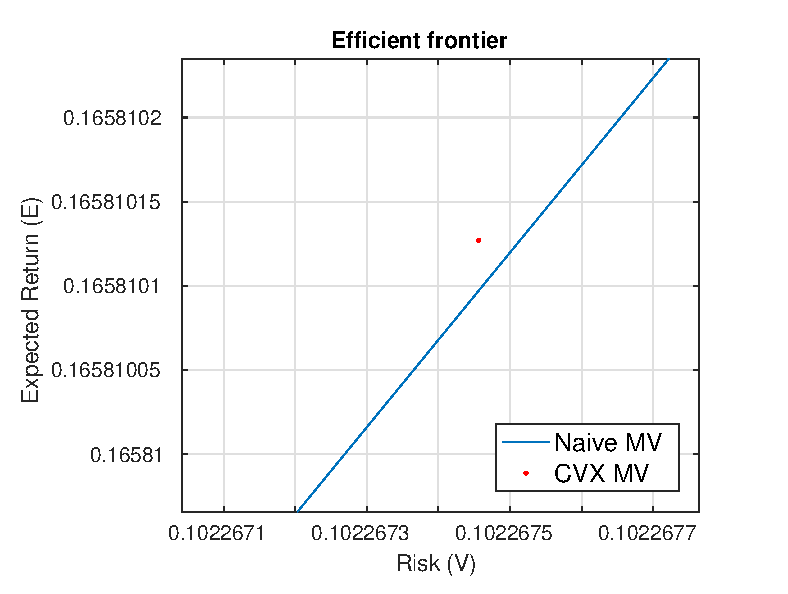
\includegraphics[scale=.5] {q1_d_naive_v_cvx_difference.eps}
       \caption{Difference}
        \label{fig:q1-d-naive-v-cvx-difference}
    \end{subfigure}
    \caption{NaiveMV vs Using CVX}\label{fig:naive_v_cvx}
\end{figure}

The results are extremely similar, since differences only show up in $10^{-7}$ scale. However, the
CVX tool was noticeably slower.

\section{Markowitz vs Naive $1/N$ Strategy on FTSE 100}

\subsection{Getting FTSE 100 Data}

\begin{figure}[!h]
   \centering 
   \begin{subfigure}[b]{0.23\textwidth}
     	\resizebox {\textwidth} {!} {% This file was created by matlab2tikz.
%
%The latest updates can be retrieved from
%  http://www.mathworks.com/matlabcentral/fileexchange/22022-matlab2tikz-matlab2tikz
%where you can also make suggestions and rate matlab2tikz.
%
\definecolor{mycolor1}{rgb}{0.00000,0.44700,0.74100}%
%
\begin{tikzpicture}

\begin{axis}[%
width=4.585in,
height=3.608in,
at={(0.769in,0.487in)},
scale only axis,
xmin=0,
xmax=1200,
xlabel style={font=\color{white!15!black}},
xlabel={Days},
ymin=5400,
ymax=7400,
ylabel style={font=\color{white!15!black}},
ylabel={Adjusted Close},
axis background/.style={fill=white},
title style={font=\bfseries},
title={FTSE 100 Over 3 Years}
]
\addplot [color=mycolor1, forget plot]
  table[row sep=crcr]{%
1	7302.399902\\
2	7268.600098\\
3	7278.899902\\
4	7258.799805\\
5	7258.799805\\
6	7258.799805\\
7	7229.5\\
8	7188.799805\\
9	7186.200195\\
10	7172.200195\\
11	7188.299805\\
12	7188.299805\\
13	7188.299805\\
14	7140.799805\\
15	7107.700195\\
16	7099.200195\\
17	7118.5\\
18	7184.5\\
19	7184.5\\
20	7184.5\\
21	7161.5\\
22	7164.399902\\
23	7150.299805\\
24	7151.200195\\
25	7198.399902\\
26	7198.399902\\
27	7198.399902\\
28	7208.399902\\
29	7247.600098\\
30	7220.399902\\
31	7327.100098\\
32	7337.799805\\
33	7337.799805\\
34	7337.799805\\
35	7292.399902\\
36	7290.5\\
37	7275.5\\
38	7237.799805\\
39	7210.100098\\
40	7210.100098\\
41	7210.100098\\
42	7195.299805\\
43	7189.700195\\
44	7177.899902\\
45	7142.799805\\
46	7142.799805\\
47	7142.799805\\
48	7142.799805\\
49	7120.299805\\
50	7106.100098\\
51	7068.200195\\
52	7068.200195\\
53	7068.200195\\
54	7068.200195\\
55	7068.200195\\
56	7063.700195\\
57	7041.399902\\
58	7044\\
59	7017.200195\\
60	7011.600098\\
61	7011.600098\\
62	7011.600098\\
63	6999\\
64	6949.200195\\
65	6968.600098\\
66	6890.399902\\
67	6954.200195\\
68	6954.200195\\
69	6954.200195\\
70	6931.600098\\
71	6902.200195\\
72	6779.799805\\
73	6746.799805\\
74	6730.700195\\
75	6730.700195\\
76	6730.700195\\
77	6752.899902\\
78	6783.799805\\
79	6772\\
80	6799.5\\
81	6840.799805\\
82	6840.799805\\
83	6840.799805\\
84	6829.200195\\
85	6817.700195\\
86	6819.700195\\
87	6778\\
88	6775.799805\\
89	6775.799805\\
90	6775.799805\\
91	6794.700195\\
92	6749.700195\\
93	6792.700195\\
94	6753.200195\\
95	6730.399902\\
96	6730.399902\\
97	6730.399902\\
98	6828\\
99	6911.799805\\
100	6843.100098\\
101	6806.899902\\
102	6693.299805\\
103	6693.299805\\
104	6693.299805\\
105	6790.5\\
106	6845.399902\\
107	6917.100098\\
108	6954.200195\\
109	6996.299805\\
110	6996.299805\\
111	6996.299805\\
112	6986.600098\\
113	6958.100098\\
114	7017.600098\\
115	6986.399902\\
116	7020.5\\
117	7020.5\\
118	7020.5\\
119	7026.899902\\
120	7021.899902\\
121	7000.100098\\
122	6947.600098\\
123	7013.600098\\
124	7013.600098\\
125	7013.600098\\
126	6977.700195\\
127	7024\\
128	7070.899902\\
129	7097.5\\
130	7044.399902\\
131	7044.399902\\
132	7044.399902\\
133	7000\\
134	7033.299805\\
135	7074.299805\\
136	6983.5\\
137	6899.299805\\
138	6899.299805\\
139	6899.299805\\
140	6919.399902\\
141	6849.399902\\
142	6807.700195\\
143	6818\\
144	6909.399902\\
145	6909.399902\\
146	6909.399902\\
147	6911.399902\\
148	6834.799805\\
149	6830.799805\\
150	6813.600098\\
151	6710.299805\\
152	6710.299805\\
153	6710.299805\\
154	6730.299805\\
155	6673.299805\\
156	6665.600098\\
157	6700.899902\\
158	6777\\
159	6777\\
160	6777\\
161	6858.700195\\
162	6846.600098\\
163	6826.100098\\
164	6879.399902\\
165	6894.600098\\
166	6894.600098\\
167	6894.600098\\
168	6746\\
169	6781.5\\
170	6820.799805\\
171	6838.100098\\
172	6838.100098\\
173	6838.100098\\
174	6838.100098\\
175	6816.899902\\
176	6835.799805\\
177	6868.5\\
178	6828.5\\
179	6859\\
180	6859\\
181	6859\\
182	6869\\
183	6859.200195\\
184	6893.899902\\
185	6941.200195\\
186	6916\\
187	6916\\
188	6916\\
189	6914.700195\\
190	6866.399902\\
191	6851.299805\\
192	6809.100098\\
193	6793.5\\
194	6793.5\\
195	6793.5\\
196	6740.200195\\
197	6634.399902\\
198	6645.399902\\
199	6694\\
200	6724.399902\\
201	6724.399902\\
202	6724.399902\\
203	6721.100098\\
204	6750.399902\\
205	6724\\
206	6710.100098\\
207	6730.5\\
208	6730.5\\
209	6730.5\\
210	6699.899902\\
211	6729\\
212	6697.399902\\
213	6695.399902\\
214	6669.200195\\
215	6669.200195\\
216	6669.200195\\
217	6654.5\\
218	6670.399902\\
219	6680.700195\\
220	6682.899902\\
221	6590.600098\\
222	6590.600098\\
223	6590.600098\\
224	6533.799805\\
225	6463.600098\\
226	6545.399902\\
227	6522.299805\\
228	6577.799805\\
229	6577.799805\\
230	6577.799805\\
231	6504.299805\\
232	6360.100098\\
233	6140.399902\\
234	5982.200195\\
235	6138.700195\\
236	6138.700195\\
237	6138.700195\\
238	6338.100098\\
239	6261.200195\\
240	6226.600098\\
241	6204\\
242	6021.100098\\
243	6021.100098\\
244	6021.100098\\
245	5950.5\\
246	5966.799805\\
247	5923.5\\
248	6045\\
249	6115.799805\\
250	6115.799805\\
251	6115.799805\\
252	6231.899902\\
253	6301.5\\
254	6284.5\\
255	6273.399902\\
256	6209.600098\\
257	6209.600098\\
258	6209.600098\\
259	6185.600098\\
260	6191.899902\\
261	6230.799805\\
262	6270.799805\\
263	6270.799805\\
264	6270.799805\\
265	6270.799805\\
266	6265.700195\\
267	6262.899902\\
268	6219.299805\\
269	6136.399902\\
270	6156.299805\\
271	6156.299805\\
272	6156.299805\\
273	6053.399902\\
274	6165.799805\\
275	6167.799805\\
276	6151.399902\\
277	6138.5\\
278	6138.5\\
279	6138.5\\
280	6104.200195\\
281	6162.5\\
282	6156.700195\\
283	6114.799805\\
284	6125.700195\\
285	6125.700195\\
286	6125.700195\\
287	6117.299805\\
288	6112\\
289	6185.600098\\
290	6241.899902\\
291	6241.899902\\
292	6241.899902\\
293	6241.899902\\
294	6322.399902\\
295	6319.899902\\
296	6284.5\\
297	6260.899902\\
298	6310.399902\\
299	6310.399902\\
300	6310.399902\\
301	6381.399902\\
302	6410.299805\\
303	6405.399902\\
304	6353.5\\
305	6343.799805\\
306	6343.799805\\
307	6343.799805\\
308	6365.100098\\
309	6362.899902\\
310	6242.399902\\
311	6200.100098\\
312	6204.399902\\
313	6204.399902\\
314	6204.399902\\
315	6136.899902\\
316	6161.600098\\
317	6091.200195\\
318	6164.700195\\
319	6146.100098\\
320	6146.100098\\
321	6146.100098\\
322	6174.899902\\
323	6203.200195\\
324	6105.899902\\
325	6106.5\\
326	6106.5\\
327	6106.5\\
328	6106.5\\
329	6106.5\\
330	6199.100098\\
331	6192.700195\\
332	6184.600098\\
333	6189.600098\\
334	6189.600098\\
335	6189.600098\\
336	6201.100098\\
337	6175.5\\
338	6140\\
339	6174.600098\\
340	6139.799805\\
341	6139.799805\\
342	6139.799805\\
343	6036.700195\\
344	6146.299805\\
345	6125.399902\\
346	6182.399902\\
347	6199.399902\\
348	6199.399902\\
349	6199.399902\\
350	6130.5\\
351	6147.100098\\
352	6152.899902\\
353	6097.100098\\
354	6096\\
355	6096\\
356	6096\\
357	6012.799805\\
358	5867.200195\\
359	5962.299805\\
360	6037.700195\\
361	5950.200195\\
362	5950.200195\\
363	5950.200195\\
364	5972\\
365	6030.299805\\
366	5862.200195\\
367	5824.299805\\
368	5707.600098\\
369	5707.600098\\
370	5707.600098\\
371	5537\\
372	5672.299805\\
373	5632.200195\\
374	5689.399902\\
375	5848.100098\\
376	5848.100098\\
377	5848.100098\\
378	5898.799805\\
379	5837.100098\\
380	5922\\
381	6060.100098\\
382	6083.799805\\
383	6083.799805\\
384	6083.799805\\
385	5931.799805\\
386	5990.399902\\
387	5911.5\\
388	5877\\
389	5900\\
390	5900\\
391	5900\\
392	5773.799805\\
393	5673.600098\\
394	5876.799805\\
395	5779.899902\\
396	5804.100098\\
397	5804.100098\\
398	5804.100098\\
399	5918.200195\\
400	5961\\
401	5929.200195\\
402	5871.799805\\
403	5912.399902\\
404	5912.399902\\
405	5912.399902\\
406	5954.100098\\
407	6073.399902\\
408	6137.200195\\
409	6093.399902\\
410	6242.299805\\
411	6242.299805\\
412	6242.299805\\
413	6242.299805\\
414	6274.100098\\
415	6314.600098\\
416	6254.600098\\
417	6254.600098\\
418	6254.600098\\
419	6254.600098\\
420	6254.600098\\
421	6241\\
422	6083.100098\\
423	6034.799805\\
424	6052.399902\\
425	6052.399902\\
426	6052.399902\\
427	6102.5\\
428	6061.200195\\
429	6017.799805\\
430	5874.100098\\
431	5952.799805\\
432	5952.799805\\
433	5952.799805\\
434	6088.100098\\
435	6126.700195\\
436	6135.200195\\
437	6223.5\\
438	6238.299805\\
439	6238.299805\\
440	6238.299805\\
441	6275\\
442	6420.899902\\
443	6395.700195\\
444	6356.100098\\
445	6375.200195\\
446	6375.200195\\
447	6375.200195\\
448	6393.100098\\
449	6337.600098\\
450	6277.200195\\
451	6305.5\\
452	6334.600098\\
453	6334.600098\\
454	6334.600098\\
455	6329.899902\\
456	6279\\
457	6268.799805\\
458	6146.399902\\
459	6118.299805\\
460	6118.299805\\
461	6118.299805\\
462	6178.700195\\
463	6297.200195\\
464	6275.299805\\
465	6295.200195\\
466	6353.799805\\
467	6353.799805\\
468	6353.799805\\
469	6364.899902\\
470	6412.899902\\
471	6383.600098\\
472	6361.799805\\
473	6361.100098\\
474	6361.100098\\
475	6361.100098\\
476	6395.799805\\
477	6437.799805\\
478	6365.299805\\
479	6417\\
480	6444.100098\\
481	6444.100098\\
482	6444.100098\\
483	6376.299805\\
484	6348.399902\\
485	6345.100098\\
486	6352.299805\\
487	6378\\
488	6378\\
489	6378\\
490	6338.700195\\
491	6269.600098\\
492	6342.299805\\
493	6371.200195\\
494	6416.200195\\
495	6416.200195\\
496	6416.200195\\
497	6374.799805\\
498	6336.399902\\
499	6326.200195\\
500	6298.899902\\
501	6130\\
502	6130\\
503	6130\\
504	6072.5\\
505	6061.600098\\
506	5909.200195\\
507	5958.899902\\
508	6109\\
509	6109\\
510	6109\\
511	5961.5\\
512	6032.200195\\
513	5935.799805\\
514	6108.700195\\
515	6104.100098\\
516	6104.100098\\
517	6104.100098\\
518	6187\\
519	6229.200195\\
520	6137.600098\\
521	6084.600098\\
522	6117.799805\\
523	6117.799805\\
524	6117.799805\\
525	6155.799805\\
526	6229\\
527	6146.100098\\
528	6074.5\\
529	6042.899902\\
530	6042.899902\\
531	6042.899902\\
532	6194.100098\\
533	6083.299805\\
534	6058.5\\
535	6247.899902\\
536	6247.899902\\
537	6247.899902\\
538	6247.899902\\
539	6192\\
540	5979.200195\\
541	6081.299805\\
542	5898.899902\\
543	6187.700195\\
544	6187.700195\\
545	6187.700195\\
546	6367.899902\\
547	6403.5\\
548	6526.299805\\
549	6550.299805\\
550	6550.700195\\
551	6550.700195\\
552	6550.700195\\
553	6568.299805\\
554	6571.200195\\
555	6664.5\\
556	6736.200195\\
557	6718.5\\
558	6718.5\\
559	6718.5\\
560	6747.100098\\
561	6752.399902\\
562	6686.600098\\
563	6688.600098\\
564	6696.299805\\
565	6696.299805\\
566	6696.299805\\
567	6668.899902\\
568	6631\\
569	6555.299805\\
570	6505.100098\\
571	6579.799805\\
572	6579.799805\\
573	6579.799805\\
574	6655\\
575	6667.299805\\
576	6769.100098\\
577	6788.700195\\
578	6775.100098\\
579	6775.100098\\
580	6775.100098\\
581	6796.5\\
582	6753.799805\\
583	6753.799805\\
584	6738\\
585	6673.399902\\
586	6673.399902\\
587	6673.399902\\
588	6581.600098\\
589	6490.700195\\
590	6432.200195\\
591	6535.700195\\
592	6585.799805\\
593	6585.799805\\
594	6585.799805\\
595	6630.5\\
596	6608.600098\\
597	6521\\
598	6620.5\\
599	6753.700195\\
600	6753.700195\\
601	6753.700195\\
602	6807.799805\\
603	6844.799805\\
604	6834.899902\\
605	6825.700195\\
606	6710.5\\
607	6710.5\\
608	6710.5\\
609	6707.899902\\
610	6680.600098\\
611	6710.100098\\
612	6710.5\\
613	6784.899902\\
614	6784.899902\\
615	6784.899902\\
616	6846.700195\\
617	6830.299805\\
618	6753.799805\\
619	6790\\
620	6804.600098\\
621	6804.600098\\
622	6804.600098\\
623	6859.200195\\
624	6950.5\\
625	6928.299805\\
626	6953.600098\\
627	6984.399902\\
628	6984.399902\\
629	6984.399902\\
630	7040.899902\\
631	7033.299805\\
632	6949\\
633	7031.700195\\
634	7031.700195\\
635	7031.700195\\
636	7031.700195\\
637	7013.5\\
638	7007.299805\\
639	6995.100098\\
640	6968.899902\\
641	6960.5\\
642	6960.5\\
643	6960.5\\
644	6973\\
645	6949.600098\\
646	6933.799805\\
647	7029.899902\\
648	7046.799805\\
649	7046.799805\\
650	7046.799805\\
651	6887\\
652	6933.700195\\
653	6927.600098\\
654	6986\\
655	6986\\
656	6986\\
657	6986\\
658	6960.600098\\
659	6946.299805\\
660	7030.5\\
661	7104\\
662	7070.700195\\
663	7070.700195\\
664	7070.700195\\
665	7053.700195\\
666	7028.200195\\
667	7062.899902\\
668	7052.100098\\
669	6994.600098\\
670	6994.600098\\
671	6994.600098\\
672	7060.5\\
673	7096.799805\\
674	7075.299805\\
675	7064.299805\\
676	7089.799805\\
677	7089.799805\\
678	7089.799805\\
679	7015.399902\\
680	6937.399902\\
681	6961.799805\\
682	6833.5\\
683	6833.5\\
684	6833.5\\
685	6833.5\\
686	6833.5\\
687	6809.5\\
688	6773\\
689	6891.399902\\
690	6855\\
691	6855\\
692	6855\\
693	6895.299805\\
694	6991\\
695	7019.700195\\
696	7037.700195\\
697	7022.5\\
698	7022.5\\
699	7022.5\\
700	6962.299805\\
701	6945.200195\\
702	6837.600098\\
703	6804.100098\\
704	6740.600098\\
705	6740.600098\\
706	6740.600098\\
707	6761.100098\\
708	6721.5\\
709	6702.799805\\
710	6876.5\\
711	6911.799805\\
712	6911.799805\\
713	6911.799805\\
714	6961.100098\\
715	6919.200195\\
716	6889.100098\\
717	6940.600098\\
718	6946.700195\\
719	6946.700195\\
720	6946.700195\\
721	6949.700195\\
722	6935.399902\\
723	6949.600098\\
724	6912.200195\\
725	6915.200195\\
726	6915.200195\\
727	6915.200195\\
728	6888.899902\\
729	6898.100098\\
730	6898.100098\\
731	6857.100098\\
732	6873.5\\
733	6873.5\\
734	6873.5\\
735	6828.100098\\
736	6818.200195\\
737	6829.100098\\
738	6837.200195\\
739	6853.399902\\
740	6853.399902\\
741	6853.399902\\
742	6865.899902\\
743	6860\\
744	6871.799805\\
745	6782.600098\\
746	6749.399902\\
747	6749.399902\\
748	6749.399902\\
749	6810.600098\\
750	6825.899902\\
751	6811.600098\\
752	6852.399902\\
753	6832.799805\\
754	6832.799805\\
755	6832.799805\\
756	6796.600098\\
757	6728\\
758	6620.100098\\
759	6585.5\\
760	6550.299805\\
761	6550.299805\\
762	6550.299805\\
763	6498.799805\\
764	6388.5\\
765	6542.200195\\
766	6501.399902\\
767	6501.100098\\
768	6501.100098\\
769	6501.100098\\
770	6570\\
771	6419.799805\\
772	6366.5\\
773	6417.200195\\
774	6547.799805\\
775	6547.799805\\
776	6547.799805\\
777	6566.100098\\
778	6566.100098\\
779	6547\\
780	6633.5\\
781	6609.899902\\
782	6609.899902\\
783	6609.899902\\
784	6609.899902\\
785	6609.899902\\
786	6598.200195\\
787	6576.700195\\
788	6545.299805\\
789	6545.299805\\
790	6545.299805\\
791	6466\\
792	6336.5\\
793	6331.799805\\
794	6182.700195\\
795	6300.600098\\
796	6300.600098\\
797	6300.600098\\
798	6461.700195\\
799	6500\\
800	6529.5\\
801	6672.200195\\
802	6742.799805\\
803	6742.799805\\
804	6742.799805\\
805	6679.399902\\
806	6716.600098\\
807	6742.100098\\
808	6656.399902\\
809	6722.600098\\
810	6722.600098\\
811	6722.600098\\
812	6723.399902\\
813	6729.200195\\
814	6731.100098\\
815	6729.799805\\
816	6750.799805\\
817	6750.799805\\
818	6750.799805\\
819	6678.899902\\
820	6696.600098\\
821	6709.100098\\
822	6672\\
823	6654.399902\\
824	6654.399902\\
825	6654.399902\\
826	6635.5\\
827	6611\\
828	6627.399902\\
829	6611.299805\\
830	6567.200195\\
831	6567.200195\\
832	6567.200195\\
833	6551.200195\\
834	6539.100098\\
835	6454\\
836	6488\\
837	6546.5\\
838	6546.5\\
839	6546.5\\
840	6463.600098\\
841	6453.899902\\
842	6402.200195\\
843	6363.5\\
844	6388.700195\\
845	6388.700195\\
846	6388.700195\\
847	6419.200195\\
848	6399.700195\\
849	6372.299805\\
850	6267.100098\\
851	6310.299805\\
852	6310.299805\\
853	6310.299805\\
854	6195.899902\\
855	6211.600098\\
856	6392.700195\\
857	6366.200195\\
858	6340\\
859	6340\\
860	6340\\
861	6431.899902\\
862	6482.200195\\
863	6495.600098\\
864	6563.700195\\
865	6527.899902\\
866	6527.899902\\
867	6527.899902\\
868	6446.399902\\
869	6557.5\\
870	6622.700195\\
871	6646.600098\\
872	6649.399902\\
873	6649.399902\\
874	6649.399902\\
875	6639.700195\\
876	6706.299805\\
877	6676.100098\\
878	6773.600098\\
879	6837.899902\\
880	6837.899902\\
881	6837.899902\\
882	6819.299805\\
883	6780.899902\\
884	6792.200195\\
885	6804.200195\\
886	6807\\
887	6807\\
888	6807\\
889	6799.600098\\
890	6830.100098\\
891	6829\\
892	6834.799805\\
893	6855.100098\\
894	6855.100098\\
895	6855.100098\\
896	6878\\
897	6873.600098\\
898	6829.200195\\
899	6825.299805\\
900	6819.799805\\
901	6819.799805\\
902	6819.799805\\
903	6805.799805\\
904	6830.700195\\
905	6822.799805\\
906	6775.299805\\
907	6775.299805\\
908	6775.299805\\
909	6775.299805\\
910	6777.700195\\
911	6755.5\\
912	6779.299805\\
913	6741.299805\\
914	6689.100098\\
915	6689.100098\\
916	6689.100098\\
917	6685.299805\\
918	6656.700195\\
919	6632.399902\\
920	6632.799805\\
921	6567.399902\\
922	6567.399902\\
923	6567.399902\\
924	6597.399902\\
925	6636.200195\\
926	6682.5\\
927	6677.5\\
928	6679.200195\\
929	6679.200195\\
930	6679.200195\\
931	6730.100098\\
932	6773.399902\\
933	6807.799805\\
934	6788.100098\\
935	6791.600098\\
936	6791.600098\\
937	6791.600098\\
938	6821.5\\
939	6798.200195\\
940	6795.299805\\
941	6728.399902\\
942	6749.5\\
943	6749.5\\
944	6749.5\\
945	6738.299805\\
946	6784.700195\\
947	6710.5\\
948	6746.100098\\
949	6690.200195\\
950	6690.200195\\
951	6690.200195\\
952	6672.399902\\
953	6718\\
954	6738.5\\
955	6823.5\\
956	6866.100098\\
957	6866.100098\\
958	6866.100098\\
959	6865.200195\\
960	6816.399902\\
961	6802.899902\\
962	6743.899902\\
963	6757.799805\\
964	6757.799805\\
965	6757.799805\\
966	6735.100098\\
967	6733.600098\\
968	6787.100098\\
969	6800.600098\\
970	6825.200195\\
971	6825.200195\\
972	6825.200195\\
973	6808.100098\\
974	6778.600098\\
975	6766.799805\\
976	6754.600098\\
977	6777.899902\\
978	6777.899902\\
979	6777.899902\\
980	6843.100098\\
981	6838.899902\\
982	6873.600098\\
983	6875\\
984	6858.200195\\
985	6858.200195\\
986	6858.200195\\
987	6813.5\\
988	6818.600098\\
989	6836.299805\\
990	6864.100098\\
991	6844.5\\
992	6844.5\\
993	6844.5\\
994	6871.299805\\
995	6851.200195\\
996	6844.899902\\
997	6815.799805\\
998	6815.799805\\
999	6815.799805\\
1000	6815.799805\\
1001	6820.600098\\
1002	6821\\
1003	6802\\
1004	6844.600098\\
1005	6855.799805\\
1006	6855.799805\\
1007	6855.799805\\
1008	6840.899902\\
1009	6878.5\\
1010	6873.100098\\
1011	6851.799805\\
1012	6814.600098\\
1013	6814.600098\\
1014	6814.600098\\
1015	6839.299805\\
1016	6796.399902\\
1017	6798.600098\\
1018	6822.399902\\
1019	6822.399902\\
1020	6822.399902\\
1021	6822.399902\\
1022	6808.899902\\
1023	6780\\
1024	6769.899902\\
1025	6700.200195\\
1026	6685.700195\\
1027	6685.700195\\
1028	6685.700195\\
1029	6703\\
1030	6674.700195\\
1031	6681.799805\\
1032	6625.299805\\
1033	6625.299805\\
1034	6625.299805\\
1035	6625.299805\\
1036	6625.299805\\
1037	6584.200195\\
1038	6541.600098\\
1039	6583.799805\\
1040	6561.700195\\
1041	6561.700195\\
1042	6561.700195\\
1043	6642\\
1044	6635.600098\\
1045	6590.700195\\
1046	6622.799805\\
1047	6695.600098\\
1048	6695.600098\\
1049	6695.600098\\
1050	6649.100098\\
1051	6659\\
1052	6652.600098\\
1053	6598.399902\\
1054	6615.600098\\
1055	6615.600098\\
1056	6615.600098\\
1057	6588.299805\\
1058	6605.299805\\
1059	6604.899902\\
1060	6520.399902\\
1061	6557.200195\\
1062	6557.200195\\
1063	6557.200195\\
1064	6542.399902\\
1065	6573.100098\\
1066	6605.299805\\
1067	6568.399902\\
1068	6527.899902\\
1069	6527.899902\\
1070	6527.899902\\
1071	6553.799805\\
1072	6620.899902\\
1073	6685.5\\
1074	6689.5\\
1075	6712.700195\\
1076	6712.700195\\
1077	6712.700195\\
1078	6788.5\\
1079	6775.399902\\
1080	6823.799805\\
1081	6708.399902\\
1082	6809.700195\\
1083	6809.700195\\
1084	6809.700195\\
1085	6810.299805\\
1086	6799.200195\\
1087	6830.5\\
};
\end{axis}
\end{tikzpicture}% }
		\label{fig:q2-ftse}
    \end{subfigure}
    ~
    \begin{subfigure}[b]{0.23\textwidth}
       	\resizebox {\textwidth} {!} {% This file was created by matlab2tikz.
%
%The latest updates can be retrieved from
%  http://www.mathworks.com/matlabcentral/fileexchange/22022-matlab2tikz-matlab2tikz
%where you can also make suggestions and rate matlab2tikz.
%
\definecolor{mycolor1}{rgb}{0.00000,0.44700,0.74100}%
\definecolor{mycolor2}{rgb}{0.85000,0.32500,0.09800}%
\definecolor{mycolor3}{rgb}{0.92900,0.69400,0.12500}%
\definecolor{mycolor4}{rgb}{0.49400,0.18400,0.55600}%
\definecolor{mycolor5}{rgb}{0.46600,0.67400,0.18800}%
\definecolor{mycolor6}{rgb}{0.30100,0.74500,0.93300}%
\definecolor{mycolor7}{rgb}{0.63500,0.07800,0.18400}%
%
\begin{tikzpicture}

\begin{axis}[%
width=4.65in,
height=3.651in,
at={(0.78in,0.493in)},
scale only axis,
xmin=0,
xmax=1200,
xlabel style={font=\color{white!15!black}},
xlabel={\huge{Days}},
ymin=0,
ymax=4000,
ylabel style={font=\color{white!15!black}},
ylabel={\huge{Adjusted Close}},
axis background/.style={fill=white},
title style={font=\bfseries},
title={\Large{FTSE 100 Top 30 Company over 3 Years}}
]
\addplot [color=mycolor1, forget plot]
  table[row sep=crcr]{%
1	1395\\
2	1391\\
3	1409.5\\
4	1352.5\\
5	1352.5\\
6	1352.5\\
7	1295.5\\
8	1331\\
9	1335.5\\
10	1329.5\\
11	1332\\
12	1332\\
13	1332\\
14	1377.5\\
15	1371.5\\
16	1358\\
17	1333\\
18	1369\\
19	1369\\
20	1369\\
21	1355.5\\
22	1361.5\\
23	1386\\
24	1308.5\\
25	1289.5\\
26	1289.5\\
27	1289.5\\
28	1302\\
29	1343\\
30	1324\\
31	1355.5\\
32	1329.5\\
33	1329.5\\
34	1329.5\\
35	1310.5\\
36	1285\\
37	1237.5\\
38	1154.5\\
39	1135\\
40	1135\\
41	1135\\
42	1145\\
43	1142.5\\
44	1162\\
45	1160\\
46	1160\\
47	1160\\
48	1160\\
49	1161\\
50	1165.5\\
51	1125.5\\
52	1125.5\\
53	1125.5\\
54	1125.5\\
55	1125.5\\
56	1126\\
57	1134.5\\
58	1135\\
59	1124.5\\
60	1133\\
61	1133\\
62	1133\\
63	1154.5\\
64	1202.5\\
65	1178.5\\
66	1210\\
67	1214\\
68	1214\\
69	1214\\
70	1245\\
71	1252\\
72	1194.5\\
73	1243\\
74	1209\\
75	1209\\
76	1209\\
77	1207.5\\
78	1185\\
79	1204.5\\
80	1237\\
81	1235.5\\
82	1235.5\\
83	1235.5\\
84	1254\\
85	1237.5\\
86	1208\\
87	1122.5\\
88	1089.5\\
89	1089.5\\
90	1089.5\\
91	1126.5\\
92	1094\\
93	1096.5\\
94	1175\\
95	1148.5\\
96	1148.5\\
97	1148.5\\
98	1176.5\\
99	1193\\
100	1153\\
101	1122.5\\
102	1071.5\\
103	1071.5\\
104	1071.5\\
105	1100\\
106	1130.5\\
107	1123.5\\
108	1131\\
109	1099.5\\
110	1099.5\\
111	1099.5\\
112	1102\\
113	1092\\
114	1114\\
115	1065.5\\
116	1094\\
117	1094\\
118	1094\\
119	1064\\
120	1054.5\\
121	1029.5\\
122	1012.5\\
123	1006\\
124	1006\\
125	1006\\
126	990.6\\
127	1040.5\\
128	1031\\
129	1042.5\\
130	1021\\
131	1021\\
132	1021\\
133	998.4\\
134	1011\\
135	986.3\\
136	995.4\\
137	967.6\\
138	967.6\\
139	967.6\\
140	980.1\\
141	923.7\\
142	916.8\\
143	930.8\\
144	951\\
145	951\\
146	951\\
147	920.5\\
148	888.7\\
149	857.6\\
150	860.9\\
151	814.4\\
152	814.4\\
153	814.4\\
154	811.5\\
155	803.6\\
156	783.8\\
157	819.5\\
158	846.6\\
159	846.6\\
160	846.6\\
161	858.9\\
162	840.2\\
163	826.8\\
164	814\\
165	808\\
166	808\\
167	808\\
168	788.7\\
169	779.8\\
170	817.5\\
171	858.5\\
172	858.5\\
173	858.5\\
174	858.5\\
175	839.6\\
176	848.6\\
177	876.1\\
178	835\\
179	870\\
180	870\\
181	870\\
182	880\\
183	865.7\\
184	890\\
185	872.7\\
186	856.9\\
187	856.9\\
188	856.9\\
189	884.9\\
190	876.9\\
191	879\\
192	875.3\\
193	859.9\\
194	859.9\\
195	859.9\\
196	845\\
197	835.4\\
198	835\\
199	848.8\\
200	830.5\\
201	830.5\\
202	830.5\\
203	842.6\\
204	799.2\\
205	782.1\\
206	775.8\\
207	775.7\\
208	775.7\\
209	775.7\\
210	787.7\\
211	774.4\\
212	813.6\\
213	832\\
214	836.1\\
215	836.1\\
216	836.1\\
217	843.4\\
218	812.2\\
219	830.5\\
220	808.9\\
221	745\\
222	745\\
223	745\\
224	746.5\\
225	730.2\\
226	739.8\\
227	764\\
228	758\\
229	758\\
230	758\\
231	726.9\\
232	696.9\\
233	644.9\\
234	629.9\\
235	659\\
236	659\\
237	659\\
238	694.7\\
239	670.5\\
240	658.3\\
241	670\\
242	636.5\\
243	636.5\\
244	636.5\\
245	612.4\\
246	631\\
247	599.5\\
248	635.4\\
249	642.5\\
250	642.5\\
251	642.5\\
252	666\\
253	697.5\\
254	665.5\\
255	686.6\\
256	617.9\\
257	617.9\\
258	617.9\\
259	587.5\\
260	592.1\\
261	600.1\\
262	612\\
263	612\\
264	612\\
265	612\\
266	629.2\\
267	620.2\\
268	608.5\\
269	598.4\\
270	600.3\\
271	600.3\\
272	600.3\\
273	579.3\\
274	606.1\\
275	628.7\\
276	609.5\\
277	578.2\\
278	578.2\\
279	578.2\\
280	575\\
281	617.3\\
282	585.8\\
283	559.5\\
284	649.4\\
285	649.4\\
286	649.4\\
287	654.6\\
288	643.2\\
289	665.7\\
290	763.4\\
291	763.4\\
292	763.4\\
293	763.4\\
294	753.2\\
295	696.9\\
296	667.2\\
297	679.1\\
298	732.8\\
299	732.8\\
300	732.8\\
301	747.3\\
302	792\\
303	752.5\\
304	693.6\\
305	678.3\\
306	678.3\\
307	678.3\\
308	690.2\\
309	709.3\\
310	638.7\\
311	585.1\\
312	547.2\\
313	547.2\\
314	547.2\\
315	506.1\\
316	522.5\\
317	525.7\\
318	547.5\\
319	538.4\\
320	538.4\\
321	538.4\\
322	552.1\\
323	535.7\\
324	479.1\\
325	500.8\\
326	500.8\\
327	500.8\\
328	500.8\\
329	500.8\\
330	523.5\\
331	553.3\\
332	549.5\\
333	555.4\\
334	555.4\\
335	555.4\\
336	540.9\\
337	492.7\\
338	487.45\\
339	546.5\\
340	515.6\\
341	515.6\\
342	515.6\\
343	502.8\\
344	530.3\\
345	530.9\\
346	628.1\\
347	592\\
348	592\\
349	592\\
350	533\\
351	524.1\\
352	491.3\\
353	480.25\\
354	450.6\\
355	450.6\\
356	450.6\\
357	422.15\\
358	409.75\\
359	453.1\\
360	483.75\\
361	436.65\\
362	436.65\\
363	436.65\\
364	432\\
365	468.05\\
366	397.95\\
367	393.05\\
368	373.95\\
369	373.95\\
370	373.95\\
371	315.95\\
372	327\\
373	333.8\\
374	376.1\\
375	363.35\\
376	363.35\\
377	363.35\\
378	328.3\\
379	273.7\\
380	252.15\\
381	274.05\\
382	277.45\\
383	277.45\\
384	277.45\\
385	275.9\\
386	253.75\\
387	253.35\\
388	226.6\\
389	226.7\\
390	226.7\\
391	226.7\\
392	248\\
393	221.05\\
394	238.8\\
395	232.65\\
396	232.75\\
397	232.75\\
398	232.75\\
399	262.95\\
400	231.45\\
401	232.5\\
402	230.45\\
403	229.2\\
404	229.2\\
405	229.2\\
406	240.65\\
407	270.4\\
408	283.2\\
409	277.85\\
410	299.45\\
411	299.45\\
412	299.45\\
413	299.45\\
414	301.8\\
415	307.35\\
416	328.05\\
417	328.05\\
418	328.05\\
419	328.05\\
420	328.05\\
421	323.35\\
422	296.5\\
423	280.5\\
424	278.65\\
425	278.65\\
426	278.65\\
427	263.55\\
428	278.2\\
429	271.1\\
430	280.8\\
431	292.95\\
432	292.95\\
433	292.95\\
434	318.65\\
435	319.7\\
436	323.65\\
437	369\\
438	376.05\\
439	376.05\\
440	376.05\\
441	386.85\\
442	397.55\\
443	406.3\\
444	408.65\\
445	400.15\\
446	400.15\\
447	400.15\\
448	435.8\\
449	417.2\\
450	452\\
451	441.15\\
452	446.5\\
453	446.5\\
454	446.5\\
455	450.75\\
456	449.45\\
457	431\\
458	454\\
459	456.2\\
460	456.2\\
461	456.2\\
462	449.9\\
463	492.75\\
464	491.75\\
465	516\\
466	525.4\\
467	525.4\\
468	525.4\\
469	534.6\\
470	579.1\\
471	561.9\\
472	544.3\\
473	546.6\\
474	546.6\\
475	546.6\\
476	537\\
477	563\\
478	557.4\\
479	590.9\\
480	609.9\\
481	609.9\\
482	609.9\\
483	596.9\\
484	604.6\\
485	623\\
486	625.5\\
487	675.3\\
488	675.3\\
489	675.3\\
490	677\\
491	681\\
492	679.2\\
493	691.7\\
494	726.5\\
495	726.5\\
496	726.5\\
497	677.5\\
498	664.5\\
499	604.2\\
500	579.5\\
501	553.6\\
502	553.6\\
503	553.6\\
504	555\\
505	550.9\\
506	543.1\\
507	552.7\\
508	614.7\\
509	614.7\\
510	614.7\\
511	624.6\\
512	658.1\\
513	648.1\\
514	694.9\\
515	720\\
516	720\\
517	720\\
518	735.4\\
519	749.3\\
520	735.2\\
521	716.9\\
522	718.4\\
523	718.4\\
524	718.4\\
525	717\\
526	742.9\\
527	703.9\\
528	677.7\\
529	668.5\\
530	668.5\\
531	668.5\\
532	725\\
533	683.8\\
534	684.4\\
535	741\\
536	741\\
537	741\\
538	741\\
539	726.3\\
540	664.3\\
541	683.7\\
542	660.2\\
543	732.8\\
544	732.8\\
545	732.8\\
546	740.5\\
547	709.4\\
548	741.9\\
549	755.2\\
550	756.8\\
551	756.8\\
552	756.8\\
553	764.9\\
554	770\\
555	774.8\\
556	808.4\\
557	800.5\\
558	800.5\\
559	800.5\\
560	775.4\\
561	777.167\\
562	763.924\\
563	758.568\\
564	789.923\\
565	789.923\\
566	789.923\\
567	784.568\\
568	792.26\\
569	775.706\\
570	752.336\\
571	757.594\\
572	757.594\\
573	757.594\\
574	785.249\\
575	792.163\\
576	839.099\\
577	844.552\\
578	854.387\\
579	854.387\\
580	854.387\\
581	866.949\\
582	851.466\\
583	846.694\\
584	855.166\\
585	840.365\\
586	840.365\\
587	840.365\\
588	836.664\\
589	823.421\\
590	810.47\\
591	860.035\\
592	878.731\\
593	878.731\\
594	878.731\\
595	894.117\\
596	886.229\\
597	894.409\\
598	923.622\\
599	934.431\\
600	934.431\\
601	934.431\\
602	968.708\\
603	981.562\\
604	970.558\\
605	969\\
606	960.723\\
607	960.723\\
608	960.723\\
609	964.715\\
610	940.274\\
611	946.701\\
612	968.318\\
613	979.614\\
614	979.614\\
615	979.614\\
616	981.075\\
617	983.509\\
618	959.554\\
619	979.127\\
620	988.865\\
621	988.865\\
622	988.865\\
623	978.64\\
624	1020.512\\
625	1020.999\\
626	976.693\\
627	999.089\\
628	999.089\\
629	999.089\\
630	1007.853\\
631	1013.209\\
632	1009.314\\
633	1034.632\\
634	1034.632\\
635	1034.632\\
636	1034.632\\
637	1031.224\\
638	1036.58\\
639	1033.171\\
640	1048.752\\
641	1061.898\\
642	1061.898\\
643	1061.898\\
644	1081.373\\
645	1101.822\\
646	1102.309\\
647	1098.414\\
648	1086.242\\
649	1086.242\\
650	1086.242\\
651	1077.965\\
652	1123.245\\
653	1135.904\\
654	1134.444\\
655	1134.444\\
656	1134.444\\
657	1134.444\\
658	1076.017\\
659	1108.639\\
660	1099.388\\
661	1074.557\\
662	1053.621\\
663	1053.621\\
664	1053.621\\
665	1034.145\\
666	987.404\\
667	990.325\\
668	1010.775\\
669	983.996\\
670	983.996\\
671	983.996\\
672	1011.748\\
673	1027.329\\
674	1012.235\\
675	972.505\\
676	995.194\\
677	995.194\\
678	995.194\\
679	997.142\\
680	999.576\\
681	998.603\\
682	970.85\\
683	970.85\\
684	970.85\\
685	970.85\\
686	970.85\\
687	989.839\\
688	985.457\\
689	1032.198\\
690	1016.617\\
691	1016.617\\
692	1016.617\\
693	1048.265\\
694	1075.53\\
695	1064.819\\
696	1084.781\\
697	1071.635\\
698	1071.635\\
699	1071.635\\
700	1018.565\\
701	989.839\\
702	991.69\\
703	976.881\\
704	976.419\\
705	976.419\\
706	976.419\\
707	998.631\\
708	1004.647\\
709	1000.945\\
710	1053.236\\
711	1051.385\\
712	1051.385\\
713	1051.385\\
714	1077.762\\
715	1080.076\\
716	1114.783\\
717	1111.544\\
718	1119.873\\
719	1119.873\\
720	1119.873\\
721	1127.278\\
722	1133.756\\
723	1144.862\\
724	1108.767\\
725	1153.655\\
726	1153.655\\
727	1153.655\\
728	1131.905\\
729	1165.224\\
730	1143.011\\
731	1129.591\\
732	1114.783\\
733	1114.783\\
734	1114.783\\
735	1078.688\\
736	1039.816\\
737	1063.417\\
738	1095.81\\
739	1060.178\\
740	1060.178\\
741	1060.178\\
742	1084.704\\
743	1064.343\\
744	1082.853\\
745	1040.279\\
746	1030.098\\
747	1030.098\\
748	1030.098\\
749	1015.753\\
750	1031.949\\
751	1008.812\\
752	1034.263\\
753	1021.306\\
754	1021.306\\
755	1021.306\\
756	1059.715\\
757	1037.965\\
758	1037.965\\
759	1008.349\\
760	1017.604\\
761	1017.604\\
762	1017.604\\
763	980.583\\
764	964.85\\
765	1060.178\\
766	1055.087\\
767	1066.656\\
768	1066.656\\
769	1066.656\\
770	1093.033\\
771	1067.119\\
772	1068.97\\
773	1042.593\\
774	1096.736\\
775	1096.736\\
776	1096.736\\
777	1111.081\\
778	1111.081\\
779	1113.858\\
780	1124.038\\
781	1093.959\\
782	1093.959\\
783	1093.959\\
784	1093.959\\
785	1093.959\\
786	1093.496\\
787	1086.092\\
788	1104.14\\
789	1104.14\\
790	1104.14\\
791	1080.076\\
792	1070.821\\
793	1053.236\\
794	1016.678\\
795	1051.385\\
796	1051.385\\
797	1051.385\\
798	1085.629\\
799	1117.56\\
800	1131.905\\
801	1151.341\\
802	1173.553\\
803	1173.553\\
804	1173.553\\
805	1187.899\\
806	1221.68\\
807	1209.186\\
808	1206.872\\
809	1223.068\\
810	1223.068\\
811	1223.068\\
812	1251.297\\
813	1247.132\\
814	1230.473\\
815	1253.148\\
816	1277.211\\
817	1277.211\\
818	1277.211\\
819	1197.154\\
820	1224.457\\
821	1261.477\\
822	1270.27\\
823	1254.073\\
824	1254.073\\
825	1254.073\\
826	1259.626\\
827	1262.866\\
828	1242.041\\
829	1259.163\\
830	1262.866\\
831	1262.866\\
832	1262.866\\
833	1230.01\\
834	1230.473\\
835	1226.77\\
836	1217.978\\
837	1218.441\\
838	1218.441\\
839	1218.441\\
840	1222.143\\
841	1251.759\\
842	1244.355\\
843	1199.931\\
844	1210.574\\
845	1210.574\\
846	1210.574\\
847	1240.19\\
848	1255.461\\
849	1272.121\\
850	1262.866\\
851	1263.328\\
852	1263.328\\
853	1263.328\\
854	1264.717\\
855	1280.45\\
856	1317.008\\
857	1284.615\\
858	1226.77\\
859	1226.77\\
860	1226.77\\
861	1254.999\\
862	1238.339\\
863	1272.583\\
864	1247.595\\
865	1216.59\\
866	1216.59\\
867	1216.59\\
868	1228.159\\
869	1261.94\\
870	1280.913\\
871	1280.913\\
872	1301.737\\
873	1301.737\\
874	1301.737\\
875	1302.2\\
876	1352.178\\
877	1322.099\\
878	1320.247\\
879	1362.358\\
880	1362.358\\
881	1362.358\\
882	1378.555\\
883	1385.496\\
884	1385.959\\
885	1377.629\\
886	1372.539\\
887	1372.539\\
888	1372.539\\
889	1383.645\\
890	1401.693\\
891	1413.262\\
892	1428.533\\
893	1447.969\\
894	1447.969\\
895	1447.969\\
896	1474.809\\
897	1462.314\\
898	1445.655\\
899	1410.022\\
900	1416.038\\
901	1416.038\\
902	1416.038\\
903	1399.842\\
904	1451.208\\
905	1459.538\\
906	1440.564\\
907	1440.564\\
908	1440.564\\
909	1440.564\\
910	1456.298\\
911	1475.271\\
912	1460.926\\
913	1479.899\\
914	1460\\
915	1460\\
916	1460\\
917	1466.016\\
918	1459.075\\
919	1467.867\\
920	1483.138\\
921	1435.474\\
922	1435.474\\
923	1435.474\\
924	1414.65\\
925	1453.059\\
926	1438.794\\
927	1448.849\\
928	1444.278\\
929	1444.278\\
930	1444.278\\
931	1461.646\\
932	1489.069\\
933	1506.437\\
934	1492.725\\
935	1498.667\\
936	1498.667\\
937	1498.667\\
938	1448.849\\
939	1459.818\\
940	1463.017\\
941	1412.742\\
942	1404.972\\
943	1404.972\\
944	1404.972\\
945	1406.8\\
946	1429.653\\
947	1383.948\\
948	1372.521\\
949	1351.954\\
950	1351.954\\
951	1351.954\\
952	1361.552\\
953	1375.721\\
954	1371.607\\
955	1380.291\\
956	1390.346\\
957	1390.346\\
958	1390.346\\
959	1394.003\\
960	1357.439\\
961	1359.267\\
962	1307.163\\
963	1308.077\\
964	1308.077\\
965	1308.077\\
966	1305.335\\
967	1304.878\\
968	1331.844\\
969	1344.184\\
970	1331.387\\
971	1331.387\\
972	1331.387\\
973	1326.816\\
974	1314.019\\
975	1299.85\\
976	1299.85\\
977	1288.881\\
978	1288.881\\
979	1288.881\\
980	1296.194\\
981	1338.7\\
982	1327.273\\
983	1345.098\\
984	1339.157\\
985	1339.157\\
986	1339.157\\
987	1329.102\\
988	1335.5\\
989	1332.758\\
990	1363.38\\
991	1332.301\\
992	1332.301\\
993	1332.301\\
994	1412.285\\
995	1396.288\\
996	1423.254\\
997	1438.263\\
998	1438.263\\
999	1438.263\\
1000	1438.263\\
1001	1405.886\\
1002	1413.656\\
1003	1401.315\\
1004	1431.024\\
1005	1427.367\\
1006	1427.367\\
1007	1427.367\\
1008	1469.873\\
1009	1500.495\\
1010	1496.839\\
1011	1500.495\\
1012	1466.217\\
1013	1466.217\\
1014	1466.217\\
1015	1452.505\\
1016	1432.852\\
1017	1409.999\\
1018	1430.567\\
1019	1430.567\\
1020	1430.567\\
1021	1430.567\\
1022	1430.11\\
1023	1446.106\\
1024	1409.999\\
1025	1388.518\\
1026	1401.315\\
1027	1401.315\\
1028	1401.315\\
1029	1431.938\\
1030	1414.113\\
1031	1406.343\\
1032	1414.113\\
1033	1414.113\\
1034	1414.113\\
1035	1414.113\\
1036	1414.113\\
1037	1406.343\\
1038	1383.948\\
1039	1410.914\\
1040	1404.972\\
1041	1404.972\\
1042	1404.972\\
1043	1415.484\\
1044	1424.168\\
1045	1441.536\\
1046	1420.512\\
1047	1430.567\\
1048	1430.567\\
1049	1430.567\\
1050	1386.233\\
1051	1411.371\\
1052	1390.803\\
1053	1395.374\\
1054	1379.377\\
1055	1379.377\\
1056	1379.377\\
1057	1359.267\\
1058	1361.095\\
1059	1369.322\\
1060	1316.304\\
1061	1315.847\\
1062	1315.847\\
1063	1315.847\\
1064	1290.252\\
1065	1269.228\\
1066	1312.574\\
1067	1307.208\\
1068	1272.772\\
1069	1272.772\\
1070	1272.772\\
1071	1262.486\\
1072	1269.641\\
1073	1283.952\\
1074	1281.716\\
1075	1308.102\\
1076	1308.102\\
1077	1308.102\\
1078	1399.781\\
1079	1359.532\\
1080	1343.879\\
1081	1322.413\\
1082	1369.37\\
1083	1369.37\\
1084	1369.37\\
1085	1351.929\\
1086	1336.276\\
1087	1342.09\\
};
\addplot [color=mycolor2, forget plot]
  table[row sep=crcr]{%
1	458.732\\
2	457.828\\
3	455.568\\
4	451.952\\
5	451.952\\
6	451.952\\
7	451.952\\
8	446.529\\
9	445.625\\
10	443.004\\
11	445.715\\
12	445.715\\
13	445.715\\
14	434.236\\
15	437.671\\
16	431.072\\
17	434.778\\
18	438.846\\
19	438.846\\
20	438.846\\
21	439.298\\
22	432.157\\
23	427.547\\
24	425.377\\
25	427.818\\
26	427.818\\
27	427.818\\
28	430.53\\
29	432.699\\
30	432.789\\
31	435.682\\
32	442.1\\
33	442.1\\
34	442.1\\
35	435.411\\
36	435.501\\
37	440.021\\
38	439.75\\
39	442.371\\
40	442.371\\
41	442.371\\
42	442.913\\
43	445.535\\
44	445.896\\
45	439.659\\
46	439.659\\
47	439.659\\
48	439.659\\
49	438.936\\
50	437.49\\
51	434.145\\
52	434.145\\
53	434.145\\
54	434.145\\
55	434.145\\
56	435.501\\
57	432.428\\
58	433.513\\
59	429.716\\
60	432.609\\
61	432.609\\
62	432.609\\
63	435.411\\
64	427.728\\
65	429.355\\
66	428.451\\
67	436.315\\
68	436.315\\
69	436.315\\
70	440.653\\
71	435.863\\
72	419.773\\
73	407.028\\
74	400.791\\
75	400.791\\
76	400.791\\
77	403.051\\
78	404.045\\
79	408.294\\
80	409.378\\
81	413.536\\
82	413.536\\
83	413.536\\
84	415.525\\
85	412.904\\
86	412.361\\
87	406.215\\
88	410.463\\
89	410.463\\
90	410.463\\
91	412.904\\
92	410.915\\
93	416.61\\
94	416.7\\
95	408.294\\
96	408.294\\
97	408.294\\
98	414.44\\
99	401.424\\
100	388.679\\
101	387.233\\
102	378.646\\
103	378.646\\
104	378.646\\
105	390.125\\
106	388.86\\
107	396.724\\
108	400.249\\
109	403.865\\
110	403.865\\
111	403.865\\
112	405.763\\
113	405.492\\
114	405.401\\
115	402.509\\
116	398.17\\
117	398.17\\
118	398.17\\
119	397.718\\
120	394.916\\
121	397.808\\
122	396.272\\
123	402.961\\
124	402.961\\
125	402.961\\
126	400.882\\
127	411.909\\
128	404.226\\
129	404.859\\
130	406.667\\
131	406.667\\
132	406.667\\
133	400.701\\
134	403.123\\
135	397.966\\
136	395.21\\
137	391.654\\
138	391.654\\
139	391.654\\
140	394.499\\
141	392.721\\
142	386.764\\
143	389.52\\
144	401.879\\
145	401.879\\
146	401.879\\
147	402.234\\
148	398.055\\
149	388.898\\
150	391.298\\
151	385.786\\
152	385.786\\
153	385.786\\
154	388.364\\
155	382.94\\
156	383.652\\
157	390.142\\
158	396.544\\
159	396.544\\
160	396.544\\
161	397.789\\
162	392.899\\
163	386.497\\
164	389.164\\
165	387.564\\
166	387.564\\
167	387.564\\
168	381.874\\
169	380.896\\
170	377.428\\
171	372.271\\
172	372.271\\
173	372.271\\
174	372.271\\
175	371.382\\
176	373.516\\
177	377.606\\
178	369.604\\
179	368.448\\
180	368.448\\
181	368.448\\
182	370.582\\
183	368.003\\
184	370.76\\
185	373.427\\
186	373.249\\
187	373.249\\
188	373.249\\
189	373.872\\
190	372.716\\
191	372.093\\
192	376.094\\
193	372.271\\
194	372.271\\
195	372.271\\
196	365.247\\
197	342.308\\
198	344.62\\
199	347.376\\
200	347.732\\
201	347.732\\
202	347.732\\
203	342.219\\
204	348.532\\
205	337.418\\
206	339.641\\
207	336.084\\
208	336.084\\
209	336.084\\
210	336.618\\
211	341.419\\
212	338.663\\
213	342.664\\
214	339.641\\
215	339.641\\
216	339.641\\
217	343.82\\
218	340.53\\
219	339.463\\
220	325.682\\
221	322.748\\
222	322.748\\
223	322.748\\
224	319.191\\
225	313.412\\
226	333.95\\
227	347.643\\
228	358.934\\
229	358.934\\
230	358.934\\
231	350.221\\
232	348.176\\
233	325.415\\
234	307.811\\
235	333.239\\
236	333.239\\
237	333.239\\
238	395.21\\
239	393.432\\
240	385.608\\
241	381.785\\
242	361.78\\
243	361.78\\
244	361.78\\
245	352.088\\
246	357.601\\
247	359.023\\
248	365.958\\
249	374.761\\
250	374.761\\
251	374.761\\
252	386.586\\
253	391.832\\
254	393.965\\
255	394.588\\
256	390.587\\
257	390.587\\
258	390.587\\
259	394.41\\
260	394.499\\
261	399.923\\
262	405.168\\
263	405.168\\
264	405.168\\
265	405.168\\
266	401.701\\
267	405.079\\
268	399.923\\
269	384.897\\
270	388.186\\
271	388.186\\
272	388.186\\
273	378.406\\
274	385.341\\
275	374.405\\
276	372.716\\
277	371.382\\
278	371.382\\
279	371.382\\
280	369.337\\
281	376.539\\
282	380.095\\
283	379.117\\
284	378.851\\
285	378.851\\
286	378.851\\
287	380.54\\
288	385.697\\
289	384.274\\
290	384.452\\
291	384.452\\
292	384.452\\
293	384.452\\
294	388.631\\
295	388.809\\
296	389.164\\
297	386.853\\
298	391.832\\
299	391.832\\
300	391.832\\
301	394.588\\
302	393.699\\
303	391.743\\
304	387.119\\
305	391.921\\
306	391.921\\
307	391.921\\
308	397.433\\
309	398.589\\
310	389.609\\
311	384.274\\
312	381.162\\
313	381.162\\
314	381.162\\
315	375.205\\
316	380.495\\
317	379.979\\
318	382.389\\
319	386.435\\
320	386.435\\
321	386.435\\
322	392.633\\
323	395.991\\
324	393.15\\
325	392.203\\
326	392.203\\
327	392.203\\
328	392.203\\
329	392.203\\
330	406.665\\
331	409.506\\
332	409.076\\
333	418.717\\
334	418.717\\
335	418.717\\
336	416.995\\
337	415.704\\
338	409.936\\
339	415.532\\
340	426.465\\
341	426.465\\
342	426.465\\
343	400.984\\
344	395.646\\
345	395.646\\
346	397.626\\
347	401.242\\
348	401.242\\
349	401.242\\
350	397.885\\
351	396.421\\
352	389.707\\
353	377.224\\
354	375.244\\
355	375.244\\
356	375.244\\
357	364.914\\
358	355.1\\
359	362.676\\
360	373.781\\
361	376.105\\
362	376.105\\
363	376.105\\
364	379.893\\
365	385.488\\
366	369.563\\
367	368.53\\
368	360.868\\
369	360.868\\
370	360.868\\
371	344.77\\
372	361.557\\
373	350.538\\
374	356.219\\
375	371.543\\
376	371.543\\
377	371.543\\
378	382.217\\
379	380.926\\
380	391.945\\
381	409.334\\
382	413.896\\
383	413.896\\
384	413.896\\
385	399.434\\
386	407.354\\
387	400.553\\
388	399.434\\
389	406.321\\
390	406.321\\
391	406.321\\
392	395.991\\
393	387.64\\
394	408.731\\
395	398.659\\
396	399.865\\
397	399.865\\
398	399.865\\
399	408.559\\
400	414.757\\
401	413.81\\
402	407.784\\
403	410.539\\
404	410.539\\
405	410.539\\
406	414.843\\
407	426.379\\
408	430.425\\
409	428.359\\
410	444.198\\
411	444.198\\
412	444.198\\
413	444.198\\
414	446.781\\
415	448.503\\
416	446.781\\
417	446.781\\
418	446.781\\
419	446.781\\
420	446.781\\
421	446.781\\
422	438.603\\
423	434.299\\
424	433.868\\
425	433.868\\
426	433.868\\
427	435.59\\
428	428.961\\
429	427.326\\
430	414.929\\
431	422.333\\
432	422.333\\
433	422.333\\
434	428.014\\
435	431.286\\
436	433.438\\
437	439.464\\
438	436.881\\
439	436.881\\
440	436.881\\
441	433.868\\
442	441.185\\
443	443.337\\
444	440.324\\
445	441.616\\
446	441.616\\
447	441.616\\
448	441.185\\
449	442.477\\
450	430.855\\
451	435.59\\
452	440.324\\
453	440.324\\
454	440.324\\
455	433.868\\
456	426.981\\
457	427.153\\
458	417.082\\
459	411.744\\
460	411.744\\
461	411.744\\
462	417.684\\
463	422.935\\
464	414.241\\
465	418.545\\
466	419.32\\
467	419.32\\
468	419.32\\
469	418.201\\
470	421.041\\
471	421.816\\
472	418.028\\
473	418.373\\
474	418.373\\
475	418.373\\
476	416.737\\
477	412.691\\
478	409.506\\
479	410.195\\
480	413.724\\
481	413.724\\
482	413.724\\
483	401.758\\
484	399.606\\
485	400.725\\
486	401.931\\
487	401.758\\
488	401.758\\
489	401.758\\
490	400.639\\
491	395.474\\
492	399.348\\
493	405.546\\
494	409.936\\
495	409.936\\
496	409.936\\
497	409.42\\
498	409.291\\
499	401.906\\
500	403.859\\
501	392.145\\
502	392.145\\
503	392.145\\
504	381.705\\
505	383.657\\
506	363.625\\
507	371.604\\
508	384.761\\
509	384.761\\
510	384.761\\
511	373.981\\
512	375.848\\
513	374.66\\
514	387.052\\
515	384.251\\
516	384.251\\
517	384.251\\
518	394.097\\
519	398.172\\
520	402.585\\
521	392.315\\
522	395.286\\
523	395.286\\
524	395.286\\
525	399.954\\
526	405.217\\
527	400.039\\
528	393.079\\
529	389.768\\
530	389.768\\
531	389.768\\
532	400.209\\
533	399.53\\
534	398.341\\
535	410.649\\
536	410.649\\
537	410.649\\
538	410.649\\
539	413.195\\
540	405.047\\
541	411.073\\
542	389.853\\
543	409.121\\
544	409.121\\
545	409.121\\
546	420.41\\
547	421.344\\
548	432.039\\
549	432.887\\
550	432.887\\
551	432.887\\
552	432.887\\
553	433.312\\
554	432.463\\
555	441.375\\
556	442.649\\
557	443.922\\
558	443.922\\
559	443.922\\
560	451.561\\
561	447.741\\
562	445.195\\
563	440.527\\
564	441.375\\
565	441.375\\
566	441.375\\
567	440.102\\
568	439.253\\
569	439.678\\
570	436.707\\
571	439.253\\
572	439.253\\
573	439.253\\
574	447.741\\
575	448.59\\
576	453.259\\
577	451.985\\
578	454.532\\
579	454.532\\
580	454.532\\
581	451.561\\
582	446.468\\
583	447.741\\
584	449.863\\
585	444.771\\
586	444.771\\
587	444.771\\
588	436.707\\
589	421.938\\
590	407.678\\
591	413.365\\
592	422.617\\
593	422.617\\
594	422.617\\
595	421.259\\
596	423.975\\
597	418.033\\
598	424.145\\
599	433.312\\
600	433.312\\
601	433.312\\
602	434.161\\
603	437.556\\
604	438.829\\
605	440.102\\
606	428.643\\
607	428.643\\
608	428.643\\
609	429.917\\
610	427.37\\
611	430.341\\
612	429.068\\
613	436.707\\
614	436.707\\
615	436.707\\
616	440.951\\
617	437.556\\
618	429.917\\
619	434.161\\
620	437.131\\
621	437.131\\
622	437.131\\
623	441.8\\
624	443.073\\
625	437.556\\
626	441.8\\
627	444.346\\
628	444.346\\
629	444.346\\
630	448.166\\
631	449.015\\
632	446.468\\
633	456.654\\
634	456.654\\
635	456.654\\
636	456.654\\
637	460.049\\
638	461.322\\
639	458.351\\
640	454.107\\
641	460.473\\
642	460.473\\
643	460.473\\
644	452.834\\
645	449.863\\
646	449.015\\
647	459.2\\
648	462.171\\
649	462.171\\
650	462.171\\
651	447.317\\
652	435.858\\
653	434.585\\
654	443.922\\
655	443.922\\
656	443.922\\
657	443.922\\
658	447.317\\
659	441.375\\
660	446.468\\
661	454.532\\
662	450.712\\
663	450.712\\
664	450.712\\
665	455.805\\
666	456.654\\
667	454.956\\
668	460.049\\
669	460.898\\
670	460.898\\
671	460.898\\
672	466.839\\
673	474.903\\
674	475.327\\
675	476.601\\
676	471.083\\
677	471.083\\
678	471.083\\
679	466.839\\
680	456.442\\
681	455.404\\
682	448.91\\
683	448.91\\
684	448.91\\
685	448.91\\
686	448.91\\
687	445.663\\
688	438.357\\
689	446.069\\
690	446.881\\
691	446.881\\
692	446.881\\
693	449.316\\
694	457.84\\
695	463.928\\
696	458.245\\
697	462.71\\
698	462.71\\
699	462.71\\
700	459.463\\
701	450.94\\
702	443.634\\
703	445.257\\
704	440.792\\
705	440.792\\
706	440.792\\
707	445.663\\
708	444.039\\
709	445.663\\
710	455.81\\
711	457.028\\
712	457.028\\
713	457.028\\
714	462.304\\
715	431.863\\
716	432.675\\
717	435.11\\
718	437.545\\
719	437.545\\
720	437.545\\
721	442.822\\
722	441.604\\
723	445.663\\
724	444.851\\
725	443.634\\
726	443.634\\
727	443.634\\
728	445.257\\
729	447.287\\
730	442.01\\
731	439.575\\
732	439.169\\
733	439.169\\
734	439.169\\
735	438.357\\
736	431.863\\
737	436.733\\
738	431.863\\
739	435.922\\
740	435.922\\
741	435.922\\
742	429.833\\
743	428.616\\
744	432.675\\
745	429.428\\
746	428.616\\
747	428.616\\
748	428.616\\
749	435.11\\
750	431.457\\
751	431.863\\
752	438.763\\
753	435.516\\
754	435.516\\
755	435.516\\
756	437.139\\
757	429.428\\
758	419.686\\
759	414.816\\
760	411.163\\
761	411.163\\
762	411.163\\
763	411.569\\
764	398.905\\
765	398.418\\
766	392.979\\
767	398.093\\
768	398.093\\
769	398.093\\
770	392.248\\
771	376.094\\
772	376.662\\
773	382.182\\
774	393.222\\
775	393.222\\
776	393.222\\
777	393.304\\
778	393.304\\
779	394.197\\
780	400.041\\
781	401.665\\
782	401.665\\
783	401.665\\
784	401.665\\
785	401.665\\
786	400.285\\
787	399.635\\
788	401.827\\
789	401.827\\
790	401.827\\
791	390.138\\
792	379.828\\
793	381.614\\
794	376.581\\
795	379.909\\
796	379.909\\
797	379.909\\
798	395.414\\
799	400.61\\
800	399.879\\
801	411.569\\
802	410.757\\
803	410.757\\
804	410.757\\
805	406.698\\
806	409.945\\
807	405.886\\
808	405.399\\
809	412.38\\
810	412.38\\
811	412.38\\
812	412.38\\
813	411.569\\
814	412.38\\
815	414.004\\
816	437.545\\
817	437.545\\
818	437.545\\
819	432.269\\
820	434.298\\
821	434.298\\
822	431.863\\
823	429.833\\
824	429.833\\
825	429.833\\
826	427.804\\
827	425.775\\
828	427.804\\
829	425.775\\
830	426.18\\
831	426.18\\
832	426.18\\
833	427.804\\
834	427.804\\
835	423.745\\
836	420.092\\
837	422.933\\
838	422.933\\
839	422.933\\
840	420.498\\
841	419.686\\
842	420.092\\
843	410.757\\
844	411.569\\
845	411.569\\
846	411.569\\
847	410.757\\
848	408.321\\
849	404.344\\
850	397.931\\
851	401.421\\
852	401.421\\
853	401.421\\
854	386.485\\
855	395.09\\
856	404.019\\
857	403.451\\
858	398.174\\
859	398.174\\
860	398.174\\
861	405.318\\
862	411.69\\
863	410.487\\
864	414.9\\
865	416.907\\
866	416.907\\
867	416.907\\
868	406.073\\
869	412.493\\
870	420.117\\
871	427.741\\
872	426.938\\
873	426.938\\
874	426.938\\
875	420.919\\
876	419.314\\
877	424.932\\
878	428.543\\
879	429.747\\
880	429.747\\
881	429.747\\
882	428.543\\
883	425.734\\
884	422.123\\
885	422.524\\
886	421.722\\
887	421.722\\
888	421.722\\
889	426.136\\
890	423.728\\
891	421.32\\
892	421.722\\
893	426.136\\
894	426.136\\
895	426.136\\
896	428.142\\
897	424.531\\
898	422.123\\
899	414.098\\
900	418.11\\
901	418.11\\
902	418.11\\
903	416.104\\
904	420.919\\
905	418.512\\
906	417.308\\
907	417.308\\
908	417.308\\
909	417.308\\
910	418.913\\
911	413.697\\
912	413.697\\
913	408.48\\
914	403.665\\
915	403.665\\
916	403.665\\
917	406.073\\
918	405.27\\
919	401.659\\
920	397.967\\
921	395.479\\
922	395.479\\
923	395.479\\
924	403.264\\
925	392.992\\
926	395.64\\
927	396.122\\
928	396.202\\
929	396.202\\
930	396.202\\
931	404.066\\
932	405.27\\
933	406.073\\
934	407.678\\
935	407.276\\
936	407.276\\
937	407.276\\
938	406.073\\
939	401.659\\
940	397.727\\
941	391.547\\
942	392.831\\
943	392.831\\
944	392.831\\
945	393.874\\
946	397.967\\
947	391.387\\
948	397.325\\
949	393.232\\
950	393.232\\
951	393.232\\
952	387.775\\
953	396.362\\
954	411.289\\
955	416.505\\
956	418.512\\
957	418.512\\
958	418.512\\
959	422.123\\
960	416.104\\
961	416.505\\
962	409.684\\
963	410.888\\
964	410.888\\
965	410.888\\
966	401.097\\
967	404.066\\
968	404.869\\
969	409.283\\
970	410.085\\
971	410.085\\
972	410.085\\
973	413.295\\
974	409.684\\
975	410.487\\
976	410.888\\
977	412.894\\
978	412.894\\
979	412.894\\
980	418.913\\
981	423.728\\
982	424.129\\
983	428.142\\
984	428.543\\
985	428.543\\
986	428.543\\
987	427.339\\
988	422.123\\
989	420.518\\
990	422.926\\
991	420.518\\
992	420.518\\
993	420.518\\
994	422.926\\
995	422.926\\
996	420.919\\
997	416.335\\
998	416.335\\
999	416.335\\
1000	416.335\\
1001	415.302\\
1002	415.703\\
1003	410.888\\
1004	410.888\\
1005	411.69\\
1006	411.69\\
1007	411.69\\
1008	412.092\\
1009	426.537\\
1010	423.728\\
1011	426.136\\
1012	420.919\\
1013	420.919\\
1014	420.919\\
1015	421.32\\
1016	422.123\\
1017	426.136\\
1018	419.715\\
1019	419.715\\
1020	419.715\\
1021	419.715\\
1022	421.32\\
1023	421.722\\
1024	414.9\\
1025	408.48\\
1026	408.881\\
1027	408.881\\
1028	408.881\\
1029	408.881\\
1030	406.073\\
1031	409.684\\
1032	408.48\\
1033	408.48\\
1034	408.48\\
1035	408.48\\
1036	408.48\\
1037	400.455\\
1038	394.356\\
1039	405.27\\
1040	400.616\\
1041	400.616\\
1042	400.616\\
1043	403.665\\
1044	401.659\\
1045	393.232\\
1046	394.276\\
1047	399.813\\
1048	399.813\\
1049	399.813\\
1050	392.43\\
1051	391.467\\
1052	387.374\\
1053	375.488\\
1054	370.135\\
1055	370.135\\
1056	370.135\\
1057	380.604\\
1058	385.564\\
1059	378.715\\
1060	375.015\\
1061	378.085\\
1062	378.085\\
1063	378.085\\
1064	388.634\\
1065	386.036\\
1066	406.975\\
1067	405.794\\
1068	399.103\\
1069	399.103\\
1070	399.103\\
1071	406.188\\
1072	411.698\\
1073	412.092\\
1074	401.071\\
1075	400.284\\
1076	400.284\\
1077	400.284\\
1078	396.742\\
1079	366.907\\
1080	364.073\\
1081	362.027\\
1082	372.811\\
1083	372.811\\
1084	372.811\\
1085	369.269\\
1086	372.339\\
1087	373.52\\
};
\addplot [color=mycolor3, forget plot]
  table[row sep=crcr]{%
1	608.5\\
2	605.5\\
3	616\\
4	612\\
5	612\\
6	612\\
7	600\\
8	599.5\\
9	598\\
10	588\\
11	583.5\\
12	583.5\\
13	583.5\\
14	583.5\\
15	582.5\\
16	582\\
17	585\\
18	592.5\\
19	592.5\\
20	592.5\\
21	596\\
22	600.5\\
23	598\\
24	600\\
25	600.5\\
26	600.5\\
27	600.5\\
28	602\\
29	605\\
30	605\\
31	611.5\\
32	611.5\\
33	611.5\\
34	611.5\\
35	617.5\\
36	610\\
37	610\\
38	597.5\\
39	605\\
40	605\\
41	605\\
42	587.5\\
43	585\\
44	591\\
45	591.5\\
46	591.5\\
47	591.5\\
48	591.5\\
49	595\\
50	599\\
51	593.5\\
52	593.5\\
53	593.5\\
54	593.5\\
55	593.5\\
56	593\\
57	596\\
58	598.5\\
59	596.5\\
60	592.5\\
61	592.5\\
62	592.5\\
63	591\\
64	589\\
65	597.5\\
66	586\\
67	600.5\\
68	600.5\\
69	600.5\\
70	604\\
71	604.5\\
72	598.5\\
73	600\\
74	594\\
75	594\\
76	594\\
77	598\\
78	600.5\\
79	601.5\\
80	603\\
81	604\\
82	604\\
83	604\\
84	608.5\\
85	603\\
86	596\\
87	597.5\\
88	593.5\\
89	593.5\\
90	593.5\\
91	597\\
92	599.5\\
93	600\\
94	593.5\\
95	590.5\\
96	590.5\\
97	590.5\\
98	612\\
99	585\\
100	548\\
101	550\\
102	539\\
103	539\\
104	539\\
105	534.5\\
106	535\\
107	538.5\\
108	542.5\\
109	542.5\\
110	542.5\\
111	542.5\\
112	544\\
113	541\\
114	540.5\\
115	540\\
116	539.5\\
117	539.5\\
118	539.5\\
119	541.5\\
120	544.9\\
121	537.517\\
122	532.594\\
123	534.563\\
124	534.563\\
125	534.563\\
126	527.672\\
127	532.594\\
128	535.548\\
129	538.993\\
130	532.102\\
131	532.102\\
132	532.102\\
133	528.656\\
134	529.641\\
135	537.024\\
136	523.242\\
137	515.858\\
138	515.858\\
139	515.858\\
140	515.858\\
141	517.827\\
142	511.92\\
143	511.428\\
144	516.351\\
145	516.351\\
146	516.351\\
147	529.149\\
148	525.211\\
149	536.04\\
150	533.579\\
151	526.195\\
152	526.195\\
153	526.195\\
154	539.978\\
155	538.009\\
156	536.04\\
157	536.532\\
158	539.485\\
159	539.485\\
160	539.485\\
161	541.947\\
162	543.916\\
163	541.454\\
164	546.869\\
165	539.485\\
166	539.485\\
167	539.485\\
168	531.118\\
169	530.133\\
170	529.641\\
171	532.102\\
172	532.102\\
173	532.102\\
174	532.102\\
175	520.288\\
176	522.257\\
177	523.734\\
178	520.288\\
179	520.781\\
180	520.781\\
181	520.781\\
182	519.304\\
183	514.382\\
184	513.397\\
185	525.211\\
186	523.242\\
187	523.242\\
188	523.242\\
189	518.812\\
190	513.397\\
191	516.843\\
192	517.335\\
193	522.75\\
194	522.75\\
195	522.75\\
196	519.796\\
197	514.874\\
198	518.32\\
199	522.75\\
200	525.703\\
201	525.703\\
202	525.703\\
203	529.641\\
204	531.118\\
205	526.195\\
206	524.719\\
207	524.226\\
208	524.226\\
209	524.226\\
210	527.672\\
211	533.579\\
212	532.102\\
213	525.703\\
214	528.656\\
215	528.656\\
216	528.656\\
217	531.118\\
218	533.579\\
219	532.594\\
220	537.024\\
221	529.149\\
222	529.149\\
223	529.149\\
224	521.765\\
225	518.32\\
226	524.719\\
227	520.288\\
228	521.765\\
229	521.765\\
230	521.765\\
231	515.858\\
232	497.646\\
233	475.889\\
234	461.614\\
235	473.33\\
236	473.33\\
237	473.33\\
238	496.169\\
239	494.692\\
240	488.293\\
241	487.112\\
242	471.361\\
243	471.361\\
244	471.361\\
245	468.013\\
246	470.179\\
247	467.62\\
248	468.899\\
249	472.05\\
250	472.05\\
251	472.05\\
252	477.957\\
253	485.242\\
254	486.324\\
255	483.962\\
256	483.273\\
257	483.273\\
258	483.273\\
259	485.143\\
260	480.418\\
261	476.086\\
262	475.495\\
263	475.495\\
264	475.495\\
265	475.495\\
266	474.806\\
267	473.723\\
268	475.397\\
269	472.247\\
270	475.988\\
271	475.988\\
272	475.988\\
273	470.475\\
274	474.216\\
275	478.744\\
276	482.485\\
277	480.221\\
278	480.221\\
279	480.221\\
280	480.221\\
281	482.78\\
282	483.273\\
283	483.47\\
284	481.402\\
285	481.402\\
286	481.402\\
287	473.133\\
288	471.065\\
289	468.801\\
290	469.884\\
291	469.884\\
292	469.884\\
293	469.884\\
294	476.48\\
295	480.516\\
296	476.775\\
297	482.288\\
298	481.796\\
299	481.796\\
300	481.796\\
301	490.853\\
302	490.262\\
303	496.985\\
304	489.782\\
305	491.703\\
306	491.703\\
307	491.703\\
308	490.262\\
309	484.02\\
310	481.619\\
311	479.218\\
312	478.354\\
313	478.354\\
314	478.354\\
315	472.112\\
316	474.224\\
317	472.976\\
318	481.619\\
319	481.619\\
320	481.619\\
321	481.619\\
322	488.822\\
323	491.703\\
324	486.901\\
325	478.738\\
326	478.738\\
327	478.738\\
328	478.738\\
329	478.738\\
330	485.941\\
331	479.026\\
332	477.874\\
333	477.394\\
334	477.394\\
335	477.394\\
336	485.941\\
337	482.099\\
338	477.49\\
339	477.778\\
340	476.817\\
341	476.817\\
342	476.817\\
343	474.512\\
344	481.139\\
345	477.009\\
346	480.659\\
347	486.901\\
348	486.901\\
349	486.901\\
350	479.89\\
351	484.5\\
352	490.743\\
353	492.663\\
354	491.703\\
355	491.703\\
356	491.703\\
357	492.183\\
358	483.54\\
359	488.342\\
360	489.782\\
361	485.461\\
362	485.461\\
363	485.461\\
364	484.98\\
365	479.506\\
366	468.654\\
367	462.604\\
368	448.583\\
369	448.583\\
370	448.583\\
371	441.476\\
372	451.848\\
373	451.272\\
374	448.967\\
375	460.011\\
376	460.011\\
377	460.011\\
378	470.383\\
379	467.022\\
380	481.139\\
381	488.822\\
382	495.544\\
383	495.544\\
384	495.544\\
385	485.461\\
386	486.901\\
387	482.579\\
388	476.145\\
389	473.168\\
390	473.168\\
391	473.168\\
392	460.203\\
393	470.575\\
394	485.941\\
395	488.822\\
396	493.143\\
397	493.143\\
398	493.143\\
399	497.945\\
400	503.707\\
401	500.826\\
402	505.628\\
403	498.906\\
404	498.906\\
405	498.906\\
406	485.461\\
407	492.183\\
408	474.416\\
409	473.936\\
410	479.794\\
411	479.794\\
412	479.794\\
413	479.794\\
414	485.461\\
415	486.901\\
416	477.586\\
417	477.586\\
418	477.586\\
419	477.586\\
420	477.586\\
421	479.122\\
422	474.032\\
423	473.84\\
424	472.976\\
425	472.976\\
426	472.976\\
427	476.625\\
428	472.88\\
429	470.575\\
430	464.237\\
431	471.055\\
432	471.055\\
433	471.055\\
434	478.93\\
435	482.099\\
436	482.099\\
437	488.342\\
438	488.342\\
439	488.342\\
440	488.342\\
441	488.822\\
442	493.143\\
443	495.064\\
444	496.024\\
445	498.906\\
446	498.906\\
447	498.906\\
448	498.425\\
449	487.381\\
450	480.659\\
451	477.298\\
452	472.496\\
453	472.496\\
454	472.496\\
455	464.909\\
456	457.706\\
457	455.017\\
458	446.278\\
459	435.618\\
460	435.618\\
461	435.618\\
462	436.963\\
463	420.925\\
464	420.636\\
465	423.71\\
466	427.359\\
467	427.359\\
468	427.359\\
469	420.54\\
470	429.952\\
471	426.399\\
472	426.303\\
473	422.845\\
474	422.845\\
475	422.845\\
476	421.597\\
477	424.958\\
478	423.806\\
479	435.81\\
480	436.002\\
481	436.002\\
482	436.002\\
483	429.856\\
484	427.071\\
485	423.206\\
486	424.997\\
487	428.767\\
488	428.767\\
489	428.767\\
490	427.071\\
491	424.62\\
492	433.857\\
493	436.308\\
494	442.057\\
495	442.057\\
496	442.057\\
497	440.455\\
498	436.214\\
499	434.611\\
500	433.009\\
501	419.625\\
502	419.625\\
503	419.625\\
504	418.117\\
505	421.981\\
506	411.801\\
507	418.965\\
508	414.723\\
509	414.723\\
510	414.723\\
511	404.355\\
512	406.617\\
513	401.056\\
514	412.933\\
515	415.1\\
516	415.1\\
517	415.1\\
518	418.588\\
519	425.846\\
520	427.354\\
521	424.62\\
522	425.751\\
523	425.751\\
524	425.751\\
525	417.74\\
526	423.866\\
527	418.305\\
528	415.195\\
529	417.457\\
530	417.457\\
531	417.457\\
532	426.788\\
533	419.813\\
534	419.059\\
535	426.223\\
536	426.223\\
537	426.223\\
538	426.223\\
539	420.284\\
540	411.707\\
541	419.342\\
542	407.183\\
543	419.153\\
544	419.153\\
545	419.153\\
546	430.653\\
547	433.103\\
548	440.926\\
549	441.869\\
550	441.398\\
551	441.398\\
552	441.398\\
553	440.361\\
554	433.574\\
555	440.644\\
556	445.922\\
557	444.414\\
558	444.414\\
559	444.414\\
560	444.414\\
561	446.299\\
562	446.77\\
563	448.75\\
564	452.614\\
565	452.614\\
566	452.614\\
567	445.922\\
568	442.623\\
569	434.234\\
570	432.349\\
571	435.365\\
572	435.365\\
573	435.365\\
574	438.193\\
575	442.811\\
576	446.205\\
577	453.934\\
578	454.688\\
579	454.688\\
580	454.688\\
581	457.515\\
582	457.327\\
583	455.253\\
584	456.478\\
585	446.676\\
586	446.676\\
587	446.676\\
588	440.361\\
589	434.423\\
590	419.907\\
591	428.202\\
592	426.317\\
593	426.317\\
594	426.317\\
595	427.259\\
596	430.935\\
597	425.28\\
598	436.119\\
599	441.303\\
600	441.303\\
601	441.303\\
602	448.09\\
603	452.803\\
604	447.053\\
605	451.483\\
606	447.147\\
607	447.147\\
608	447.147\\
609	445.262\\
610	446.016\\
611	453.557\\
612	454.311\\
613	461.003\\
614	461.003\\
615	461.003\\
616	462.511\\
617	464.302\\
618	461.003\\
619	465.433\\
620	469.674\\
621	469.674\\
622	469.674\\
623	476.461\\
624	483.53\\
625	481.645\\
626	486.829\\
627	485.415\\
628	485.415\\
629	485.415\\
630	491.541\\
631	492.955\\
632	484.944\\
633	485.886\\
634	485.886\\
635	485.886\\
636	485.886\\
637	483.53\\
638	479.76\\
639	479.76\\
640	473.162\\
641	474.576\\
642	474.576\\
643	474.576\\
644	473.162\\
645	471.277\\
646	469.391\\
647	480.702\\
648	480.231\\
649	480.231\\
650	480.231\\
651	469.014\\
652	471.748\\
653	474.104\\
654	474.576\\
655	474.576\\
656	474.576\\
657	474.576\\
658	478.817\\
659	478.346\\
660	476.461\\
661	484.472\\
662	485.415\\
663	485.415\\
664	485.415\\
665	474.576\\
666	477.874\\
667	480.702\\
668	480.231\\
669	483.53\\
670	483.53\\
671	483.53\\
672	486.357\\
673	490.316\\
674	487.093\\
675	493.999\\
676	496.762\\
677	496.762\\
678	496.762\\
679	493.078\\
680	489.856\\
681	486.633\\
682	482.95\\
683	482.95\\
684	482.95\\
685	482.95\\
686	482.95\\
687	482.49\\
688	482.029\\
689	484.791\\
690	488.014\\
691	488.014\\
692	488.014\\
693	490.316\\
694	498.603\\
695	499.524\\
696	497.222\\
697	502.286\\
698	502.286\\
699	502.286\\
700	503.667\\
701	502.286\\
702	494.46\\
703	495.38\\
704	490.316\\
705	490.316\\
706	490.316\\
707	492.618\\
708	493.539\\
709	491.237\\
710	490.777\\
711	494.46\\
712	494.46\\
713	494.46\\
714	492.618\\
715	491.237\\
716	485.252\\
717	488.935\\
718	489.856\\
719	489.856\\
720	489.856\\
721	490.777\\
722	494.92\\
723	493.539\\
724	491.697\\
725	488.014\\
726	488.014\\
727	488.014\\
728	483.871\\
729	480.648\\
730	479.267\\
731	479.727\\
732	481.569\\
733	481.569\\
734	481.569\\
735	486.173\\
736	483.41\\
737	481.108\\
738	473.742\\
739	476.504\\
740	476.504\\
741	476.504\\
742	475.584\\
743	485.712\\
744	479.267\\
745	466.836\\
746	467.297\\
747	467.297\\
748	467.297\\
749	475.123\\
750	472.361\\
751	465.915\\
752	471.44\\
753	477.886\\
754	477.886\\
755	477.886\\
756	476.965\\
757	462.232\\
758	453.117\\
759	449.986\\
760	445.474\\
761	445.474\\
762	445.474\\
763	441.607\\
764	431.478\\
765	437.463\\
766	432.951\\
767	430.65\\
768	430.65\\
769	430.65\\
770	431.754\\
771	426.046\\
772	420.521\\
773	425.401\\
774	432.031\\
775	432.031\\
776	432.031\\
777	434.609\\
778	434.609\\
779	432.583\\
780	437.924\\
781	436.543\\
782	436.543\\
783	436.543\\
784	436.543\\
785	436.543\\
786	435.806\\
787	433.964\\
788	426.046\\
789	426.046\\
790	426.046\\
791	425.401\\
792	414.444\\
793	414.168\\
794	400.54\\
795	407.262\\
796	407.262\\
797	407.262\\
798	418.863\\
799	424.48\\
800	430.65\\
801	441.791\\
802	443.54\\
803	443.54\\
804	443.54\\
805	442.62\\
806	440.962\\
807	441.423\\
808	437.555\\
809	442.988\\
810	442.988\\
811	442.988\\
812	440.686\\
813	436.266\\
814	435.069\\
815	428.348\\
816	428.255\\
817	428.255\\
818	428.255\\
819	423.559\\
820	426.322\\
821	426.138\\
822	424.849\\
823	423.652\\
824	423.652\\
825	423.652\\
826	423.744\\
827	424.112\\
828	425.861\\
829	425.401\\
830	420.521\\
831	420.521\\
832	420.521\\
833	420.061\\
834	418.771\\
835	415.272\\
836	421.442\\
837	422.362\\
838	422.362\\
839	422.362\\
840	416.193\\
841	410.761\\
842	407.538\\
843	407.354\\
844	406.525\\
845	406.525\\
846	406.525\\
847	408.551\\
848	406.157\\
849	401.908\\
850	398.473\\
851	401.275\\
852	401.275\\
853	401.275\\
854	397.659\\
855	395.219\\
856	405.524\\
857	402.36\\
858	401.998\\
859	401.998\\
860	401.998\\
861	400.371\\
862	408.417\\
863	407.241\\
864	417.276\\
865	416.01\\
866	416.01\\
867	416.01\\
868	410.225\\
869	418.722\\
870	426.225\\
871	425.05\\
872	424.236\\
873	424.236\\
874	424.236\\
875	418.36\\
876	421.615\\
877	421.886\\
878	429.479\\
879	426.406\\
880	426.406\\
881	426.406\\
882	422.7\\
883	416.733\\
884	412.846\\
885	414.112\\
886	414.925\\
887	414.925\\
888	414.925\\
889	413.117\\
890	411.309\\
891	409.14\\
892	407.422\\
893	412.033\\
894	412.033\\
895	412.033\\
896	411.671\\
897	409.953\\
898	411.581\\
899	412.213\\
900	402.36\\
901	402.36\\
902	402.36\\
903	400.281\\
904	400.552\\
905	398.654\\
906	396.936\\
907	396.936\\
908	396.936\\
909	396.936\\
910	399.377\\
911	397.117\\
912	396.846\\
913	396.665\\
914	395.038\\
915	395.038\\
916	395.038\\
917	395.038\\
918	393.863\\
919	391.422\\
920	387.444\\
921	380.936\\
922	380.936\\
923	380.936\\
924	380.484\\
925	381.749\\
926	385.636\\
927	384.732\\
928	385.184\\
929	385.184\\
930	385.184\\
931	386.721\\
932	384.19\\
933	384.642\\
934	386.088\\
935	386.36\\
936	386.36\\
937	386.36\\
938	387.896\\
939	384.28\\
940	383.015\\
941	379.67\\
942	377.139\\
943	377.139\\
944	377.139\\
945	378.314\\
946	381.749\\
947	376.416\\
948	377.862\\
949	377.32\\
950	377.32\\
951	377.32\\
952	378.857\\
953	376.597\\
954	379.67\\
955	385.456\\
956	388.168\\
957	388.168\\
958	388.168\\
959	386.631\\
960	383.919\\
961	390.97\\
962	391.331\\
963	390.156\\
964	390.156\\
965	390.156\\
966	384.19\\
967	382.292\\
968	384.913\\
969	382.925\\
970	386.902\\
971	386.902\\
972	386.902\\
973	383.467\\
974	377.41\\
975	377.41\\
976	378.224\\
977	385.184\\
978	385.184\\
979	385.184\\
980	385.817\\
981	384.913\\
982	388.981\\
983	389.252\\
984	386.179\\
985	386.179\\
986	386.179\\
987	382.925\\
988	383.467\\
989	383.829\\
990	386.902\\
991	382.473\\
992	382.473\\
993	382.473\\
994	381.749\\
995	379.309\\
996	376.054\\
997	373.788\\
998	373.788\\
999	373.788\\
1000	373.788\\
1001	373.523\\
1002	371.534\\
1003	369.274\\
1004	373.523\\
1005	374.789\\
1006	374.789\\
1007	374.789\\
1008	376.506\\
1009	372.258\\
1010	370.088\\
1011	368.642\\
1012	366.111\\
1013	366.111\\
1014	366.111\\
1015	366.653\\
1016	365.659\\
1017	359.24\\
1018	362.585\\
1019	362.585\\
1020	362.585\\
1021	362.585\\
1022	362.675\\
1023	361.591\\
1024	360.868\\
1025	362.495\\
1026	363.308\\
1027	363.308\\
1028	363.308\\
1029	358.336\\
1030	357.432\\
1031	354.359\\
1032	351.737\\
1033	351.737\\
1034	351.737\\
1035	351.737\\
1036	351.737\\
1037	339.895\\
1038	343.33\\
1039	346.572\\
1040	349.2\\
1041	349.2\\
1042	349.2\\
1043	355.245\\
1044	354.194\\
1045	351.478\\
1046	355.332\\
1047	359.8\\
1048	359.8\\
1049	359.8\\
1050	356.734\\
1051	362.166\\
1052	362.954\\
1053	362.867\\
1054	356.909\\
1055	356.909\\
1056	356.909\\
1057	359.625\\
1058	360.151\\
1059	360.501\\
1060	353.493\\
1061	360.063\\
1062	360.063\\
1063	360.063\\
1064	365.407\\
1065	362.253\\
1066	357.26\\
1067	347.36\\
1068	340.001\\
1069	340.001\\
1070	340.001\\
1071	343.418\\
1072	351.215\\
1073	356.471\\
1074	352.792\\
1075	354.982\\
1076	354.982\\
1077	354.982\\
1078	362.253\\
1079	365.845\\
1080	368.298\\
1081	358.749\\
1082	359.976\\
1083	359.976\\
1084	359.976\\
1085	360.151\\
1086	359.1\\
1087	359.976\\
};
\addplot [color=mycolor4, forget plot]
  table[row sep=crcr]{%
1	239.25\\
2	235.25\\
3	232.35\\
4	228.65\\
5	228.65\\
6	228.65\\
7	229.55\\
8	224.95\\
9	226.05\\
10	227.4\\
11	228.85\\
12	228.85\\
13	228.85\\
14	221.35\\
15	222.1\\
16	219.45\\
17	223.4\\
18	230.6\\
19	230.6\\
20	230.6\\
21	232.35\\
22	230.85\\
23	228.65\\
24	224.5\\
25	227.4\\
26	227.4\\
27	227.4\\
28	228.3\\
29	227.6\\
30	231.6\\
31	231.1\\
32	235.25\\
33	235.25\\
34	235.25\\
35	232.25\\
36	234.2\\
37	236.25\\
38	234.05\\
39	235.25\\
40	235.25\\
41	235.25\\
42	232.55\\
43	235\\
44	231.9\\
45	223.45\\
46	223.45\\
47	223.45\\
48	223.45\\
49	222.35\\
50	224.75\\
51	224.95\\
52	224.95\\
53	224.95\\
54	224.95\\
55	224.95\\
56	227\\
57	228.75\\
58	227.65\\
59	222.05\\
60	228.15\\
61	228.15\\
62	228.15\\
63	229.45\\
64	221.75\\
65	230.1\\
66	227.55\\
67	233.1\\
68	233.1\\
69	233.1\\
70	239\\
71	234.85\\
72	226.75\\
73	216.8\\
74	212.95\\
75	212.95\\
76	212.95\\
77	219.05\\
78	215.95\\
79	214.25\\
80	211.9\\
81	215.5\\
82	215.5\\
83	215.5\\
84	215.45\\
85	213.35\\
86	212.35\\
87	210.6\\
88	212.25\\
89	212.25\\
90	212.25\\
91	212.7\\
92	209.6\\
93	211.9\\
94	212.3\\
95	201.75\\
96	201.75\\
97	201.75\\
98	201.1\\
99	192.9\\
100	185.95\\
101	185.2\\
102	181.35\\
103	181.35\\
104	181.35\\
105	185.3\\
106	182.05\\
107	186.7\\
108	190.3\\
109	191.3\\
110	191.3\\
111	191.3\\
112	190.5\\
113	181.8\\
114	183.7\\
115	183.5\\
116	183.2\\
117	183.2\\
118	183.2\\
119	183.1\\
120	177.4\\
121	174\\
122	169.55\\
123	170.15\\
124	170.15\\
125	170.15\\
126	166.5\\
127	168.45\\
128	172.4\\
129	172.3\\
130	173.6\\
131	173.6\\
132	173.6\\
133	174.25\\
134	172.45\\
135	169.25\\
136	168.2\\
137	167.8\\
138	167.8\\
139	167.8\\
140	167.3\\
141	166.1\\
142	165.95\\
143	168.1\\
144	171.4\\
145	171.4\\
146	171.4\\
147	173.2\\
148	171.6\\
149	166.45\\
150	167\\
151	164.7\\
152	164.7\\
153	164.7\\
154	169.5\\
155	170.3\\
156	170.6\\
157	170.05\\
158	174.75\\
159	174.75\\
160	174.75\\
161	173.2\\
162	169.75\\
163	169.7\\
164	173.25\\
165	174.3\\
166	174.3\\
167	174.3\\
168	171.55\\
169	172.25\\
170	169.15\\
171	166\\
172	166\\
173	166\\
174	166\\
175	164.35\\
176	166.55\\
177	164.6\\
178	160.05\\
179	160.35\\
180	160.35\\
181	160.35\\
182	160.65\\
183	160.15\\
184	161.75\\
185	163.55\\
186	163.4\\
187	163.4\\
188	163.4\\
189	163.25\\
190	162.7\\
191	160.215\\
192	156.438\\
193	151.071\\
194	151.071\\
195	151.071\\
196	147.941\\
197	147.394\\
198	145.108\\
199	150.475\\
200	153.606\\
201	153.606\\
202	153.606\\
203	145.605\\
204	148.835\\
205	148.09\\
206	150.078\\
207	150.873\\
208	150.873\\
209	150.873\\
210	150.972\\
211	150.028\\
212	149.481\\
213	150.028\\
214	148.885\\
215	148.885\\
216	148.885\\
217	147.096\\
218	144.214\\
219	147.643\\
220	144.512\\
221	138.399\\
222	138.399\\
223	138.399\\
224	133.927\\
225	130.846\\
226	135.02\\
227	135.716\\
228	139.145\\
229	139.145\\
230	139.145\\
231	137.753\\
232	137.107\\
233	130.697\\
234	126.423\\
235	152.96\\
236	152.96\\
237	152.96\\
238	185.808\\
239	180.888\\
240	179.248\\
241	175.77\\
242	164.737\\
243	164.737\\
244	164.737\\
245	157.532\\
246	159.967\\
247	159.072\\
248	164.141\\
249	168.365\\
250	168.365\\
251	168.365\\
252	174.975\\
253	176.962\\
254	179.149\\
255	179\\
256	178.553\\
257	178.553\\
258	178.553\\
259	179.298\\
260	178.851\\
261	181.286\\
262	185.063\\
263	185.063\\
264	185.063\\
265	185.063\\
266	183.671\\
267	184.615\\
268	180.292\\
269	174.627\\
270	174.776\\
271	174.776\\
272	174.776\\
273	169.608\\
274	169.359\\
275	163.247\\
276	162.501\\
277	164.34\\
278	164.34\\
279	164.34\\
280	161.855\\
281	162.601\\
282	162.302\\
283	157.482\\
284	161.01\\
285	161.01\\
286	161.01\\
287	159.967\\
288	161.458\\
289	163.744\\
290	170.452\\
291	170.452\\
292	170.452\\
293	170.452\\
294	173.335\\
295	173.732\\
296	172.887\\
297	169.309\\
298	170.452\\
299	170.452\\
300	170.452\\
301	170.9\\
302	170.104\\
303	166.775\\
304	166.676\\
305	165.88\\
306	165.88\\
307	165.88\\
308	167.968\\
309	165.781\\
310	154.699\\
311	152.562\\
312	149.779\\
313	149.779\\
314	149.779\\
315	146.201\\
316	148.636\\
317	145.704\\
318	149.332\\
319	149.084\\
320	149.084\\
321	149.084\\
322	149.084\\
323	150.724\\
324	150.078\\
325	151.668\\
326	151.668\\
327	151.668\\
328	151.668\\
329	151.668\\
330	155.494\\
331	156.24\\
332	159.52\\
333	161.209\\
334	161.209\\
335	161.209\\
336	159.619\\
337	162.998\\
338	162.551\\
339	162.253\\
340	164.986\\
341	164.986\\
342	164.986\\
343	158.923\\
344	163.694\\
345	167.392\\
346	169.047\\
347	169.63\\
348	169.63\\
349	169.63\\
350	161.845\\
351	158.049\\
352	153.864\\
353	167.441\\
354	164.57\\
355	164.57\\
356	164.57\\
357	160.434\\
358	152.551\\
359	157.222\\
360	160.726\\
361	157.368\\
362	157.368\\
363	157.368\\
364	157.417\\
365	163.645\\
366	157.125\\
367	156.443\\
368	152.989\\
369	152.989\\
370	152.989\\
371	143.889\\
372	154.74\\
373	152.064\\
374	159.509\\
375	168.511\\
376	168.511\\
377	168.511\\
378	168.998\\
379	161.164\\
380	169.095\\
381	177.903\\
382	181.017\\
383	181.017\\
384	181.017\\
385	173.621\\
386	176.93\\
387	178.097\\
388	176.978\\
389	185.64\\
390	185.64\\
391	185.64\\
392	181.163\\
393	177.173\\
394	184.813\\
395	182.623\\
396	186.662\\
397	186.662\\
398	186.662\\
399	192.404\\
400	196.296\\
401	196.929\\
402	194.35\\
403	194.788\\
404	194.788\\
405	194.788\\
406	200.043\\
407	206.077\\
408	209.483\\
409	208.51\\
410	213.036\\
411	213.036\\
412	213.036\\
413	213.036\\
414	214.787\\
415	216.637\\
416	215.761\\
417	215.761\\
418	215.761\\
419	215.761\\
420	215.761\\
421	216.345\\
422	213.133\\
423	210.603\\
424	211.77\\
425	211.77\\
426	211.77\\
427	212.89\\
428	209.97\\
429	209.045\\
430	203.498\\
431	205.542\\
432	205.542\\
433	205.542\\
434	212.16\\
435	216.004\\
436	216.15\\
437	221.892\\
438	223.449\\
439	223.449\\
440	223.449\\
441	224.13\\
442	228.461\\
443	227.244\\
444	217.22\\
445	218.291\\
446	218.291\\
447	218.291\\
448	219.167\\
449	215.566\\
450	214.155\\
451	214.641\\
452	215.955\\
453	215.955\\
454	215.955\\
455	223.79\\
456	221.795\\
457	221.357\\
458	218.388\\
459	219.07\\
460	219.07\\
461	219.07\\
462	219.653\\
463	225.882\\
464	224.422\\
465	227.78\\
466	226.174\\
467	226.174\\
468	226.174\\
469	222.038\\
470	225.152\\
471	226.266\\
472	228.737\\
473	224.813\\
474	224.813\\
475	224.813\\
476	229.9\\
477	245.308\\
478	243.079\\
479	243.176\\
480	243.467\\
481	243.467\\
482	243.467\\
483	242.885\\
484	240.366\\
485	244.775\\
486	246.761\\
487	243.031\\
488	243.031\\
489	243.031\\
490	240.317\\
491	238.428\\
492	243.612\\
493	248.602\\
494	249.038\\
495	249.038\\
496	249.038\\
497	246.858\\
498	247.827\\
499	247.44\\
500	248.263\\
501	240.85\\
502	240.85\\
503	240.85\\
504	239.494\\
505	236.587\\
506	231.596\\
507	237.604\\
508	247.052\\
509	247.052\\
510	247.052\\
511	238.815\\
512	240.511\\
513	239.009\\
514	247.004\\
515	245.405\\
516	245.405\\
517	245.405\\
518	252.382\\
519	254.368\\
520	251.606\\
521	246.616\\
522	250.444\\
523	250.444\\
524	250.444\\
525	250.589\\
526	254.368\\
527	250.492\\
528	245.162\\
529	243.127\\
530	243.127\\
531	243.127\\
532	249.329\\
533	245.938\\
534	245.308\\
535	253.351\\
536	253.351\\
537	253.351\\
538	253.351\\
539	254.465\\
540	244.193\\
541	248.409\\
542	237.119\\
543	248.845\\
544	248.845\\
545	248.845\\
546	256.936\\
547	259.601\\
548	265.56\\
549	265.463\\
550	265.851\\
551	265.851\\
552	265.851\\
553	267.014\\
554	262.75\\
555	269.727\\
556	273.845\\
557	272.537\\
558	272.537\\
559	272.537\\
560	273.264\\
561	272.295\\
562	272.44\\
563	278.282\\
564	279.006\\
565	279.006\\
566	279.006\\
567	277.171\\
568	274.805\\
569	269.978\\
570	267.274\\
571	272.44\\
572	272.44\\
573	272.44\\
574	272.054\\
575	271.716\\
576	273.405\\
577	271.185\\
578	270.46\\
579	270.46\\
580	270.46\\
581	270.364\\
582	268.481\\
583	266.501\\
584	264.281\\
585	258.825\\
586	258.825\\
587	258.825\\
588	252.163\\
589	248.445\\
590	243.472\\
591	249.893\\
592	253.901\\
593	253.901\\
594	253.901\\
595	257.232\\
596	257.377\\
597	251.535\\
598	255.156\\
599	262.977\\
600	262.977\\
601	262.977\\
602	263.508\\
603	265.005\\
604	263.074\\
605	263.074\\
606	256.604\\
607	256.604\\
608	256.604\\
609	252.549\\
610	252.887\\
611	254.576\\
612	255.832\\
613	260.418\\
614	260.418\\
615	260.418\\
616	259.501\\
617	257.956\\
618	252.549\\
619	252.983\\
620	256.315\\
621	256.315\\
622	256.315\\
623	257.232\\
624	261.867\\
625	258.439\\
626	257.232\\
627	260.708\\
628	260.708\\
629	260.708\\
630	261.77\\
631	259.984\\
632	255.783\\
633	260.853\\
634	260.853\\
635	260.853\\
636	260.853\\
637	261.722\\
638	262.205\\
639	253.659\\
640	252.163\\
641	252.645\\
642	252.645\\
643	252.645\\
644	253.08\\
645	251.293\\
646	248.59\\
647	251.825\\
648	249.169\\
649	249.169\\
650	249.169\\
651	240.334\\
652	239.9\\
653	240.621\\
654	244.612\\
655	244.612\\
656	244.612\\
657	244.612\\
658	245.526\\
659	247.112\\
660	251.392\\
661	253.652\\
662	251.729\\
663	251.729\\
664	251.729\\
665	248.555\\
666	243.602\\
667	245.237\\
668	247.401\\
669	245.526\\
670	245.526\\
671	245.526\\
672	250.382\\
673	249.709\\
674	252.113\\
675	249.517\\
676	247.209\\
677	247.209\\
678	247.209\\
679	248.074\\
680	246.151\\
681	248.122\\
682	244.997\\
683	244.997\\
684	244.997\\
685	244.997\\
686	244.997\\
687	239.755\\
688	233.312\\
689	238.313\\
690	234.899\\
691	234.899\\
692	234.899\\
693	240.429\\
694	242.256\\
695	248.555\\
696	247.305\\
697	245.526\\
698	245.526\\
699	245.526\\
700	243.121\\
701	242.689\\
702	240.429\\
703	242.208\\
704	240.429\\
705	240.429\\
706	240.429\\
707	244.756\\
708	245.237\\
709	244.564\\
710	249.276\\
711	251.459\\
712	251.459\\
713	251.459\\
714	252.408\\
715	248.992\\
716	241.306\\
717	249.324\\
718	243.773\\
719	243.773\\
720	243.773\\
721	248.707\\
722	249.466\\
723	250.51\\
724	249.419\\
725	248.138\\
726	248.138\\
727	248.138\\
728	247.094\\
729	247.046\\
730	244.389\\
731	245.576\\
732	243.346\\
733	243.346\\
734	243.346\\
735	240.404\\
736	238.174\\
737	240.262\\
738	240.689\\
739	242.397\\
740	242.397\\
741	242.397\\
742	236.087\\
743	236.039\\
744	235.754\\
745	223.798\\
746	222.185\\
747	222.185\\
748	222.185\\
749	224.463\\
750	224.747\\
751	227.214\\
752	228.448\\
753	230.725\\
754	230.725\\
755	230.725\\
756	230.963\\
757	225.744\\
758	223.229\\
759	218.247\\
760	212.886\\
761	212.886\\
762	212.886\\
763	216.302\\
764	212.127\\
765	221.094\\
766	219.576\\
767	219.196\\
768	219.196\\
769	219.196\\
770	224.937\\
771	218.817\\
772	218.579\\
773	222.707\\
774	230.725\\
775	230.725\\
776	230.725\\
777	231.057\\
778	231.057\\
779	229.065\\
780	230.061\\
781	230.725\\
782	230.725\\
783	230.725\\
784	230.725\\
785	230.725\\
786	230.63\\
787	228.068\\
788	225.554\\
789	225.554\\
790	225.554\\
791	222.707\\
792	216.444\\
793	218.39\\
794	213.693\\
795	220.43\\
796	220.43\\
797	220.43\\
798	225.127\\
799	225.554\\
800	226.313\\
801	234.521\\
802	236.703\\
803	236.703\\
804	236.703\\
805	230.251\\
806	231.342\\
807	232.813\\
808	228.875\\
809	232.623\\
810	232.623\\
811	232.623\\
812	231.342\\
813	225.838\\
814	226.171\\
815	225.032\\
816	224.178\\
817	224.178\\
818	224.178\\
819	222.043\\
820	223.846\\
821	225.364\\
822	222.233\\
823	220.145\\
824	220.145\\
825	220.145\\
826	217.156\\
827	217.773\\
828	222.612\\
829	222.755\\
830	222.185\\
831	222.185\\
832	222.185\\
833	224.273\\
834	224.937\\
835	223.661\\
836	223.945\\
837	227.536\\
838	227.536\\
839	227.536\\
840	210.291\\
841	208.354\\
842	210.716\\
843	209.629\\
844	213.882\\
845	213.882\\
846	213.882\\
847	213.456\\
848	211.094\\
849	211.094\\
850	206.322\\
851	201.361\\
852	201.361\\
853	201.361\\
854	196.448\\
855	200.511\\
856	209.771\\
857	211.094\\
858	211.566\\
859	211.566\\
860	211.566\\
861	213.504\\
862	216.763\\
863	217.945\\
864	219.504\\
865	212.228\\
866	212.228\\
867	212.228\\
868	208.637\\
869	214.779\\
870	214.921\\
871	213.551\\
872	215.204\\
873	215.204\\
874	215.204\\
875	215.11\\
876	216.197\\
877	216.622\\
878	218.89\\
879	221.252\\
880	221.252\\
881	221.252\\
882	221.63\\
883	218.984\\
884	217\\
885	216.763\\
886	217.33\\
887	217.33\\
888	217.33\\
889	213.078\\
890	215.677\\
891	213.456\\
892	212.511\\
893	213.787\\
894	213.787\\
895	213.787\\
896	218.039\\
897	215.535\\
898	210.102\\
899	211.755\\
900	212.086\\
901	212.086\\
902	212.086\\
903	211.708\\
904	213.456\\
905	212.842\\
906	210.527\\
907	210.527\\
908	210.527\\
909	210.527\\
910	208.637\\
911	208.543\\
912	209.015\\
913	207.503\\
914	205.613\\
915	205.613\\
916	205.613\\
917	205.991\\
918	207.267\\
919	205.047\\
920	204.338\\
921	202.401\\
922	202.401\\
923	202.401\\
924	201.645\\
925	205.566\\
926	208.732\\
927	210.66\\
928	210.942\\
929	210.942\\
930	210.942\\
931	212.306\\
932	214.846\\
933	206.098\\
934	205.204\\
935	205.11\\
936	205.11\\
937	205.11\\
938	201.771\\
939	198.432\\
940	198.102\\
941	197.726\\
942	199.231\\
943	199.231\\
944	199.231\\
945	197.726\\
946	203.182\\
947	198.149\\
948	197.162\\
949	195.563\\
950	195.563\\
951	195.563\\
952	195.657\\
953	198.949\\
954	201.018\\
955	203.229\\
956	205.581\\
957	205.581\\
958	205.581\\
959	206.333\\
960	204.217\\
961	203.182\\
962	200.172\\
963	203.229\\
964	203.229\\
965	203.229\\
966	202.241\\
967	216.351\\
968	219.831\\
969	220.396\\
970	220.678\\
971	220.678\\
972	220.678\\
973	222.183\\
974	221.525\\
975	222.465\\
976	222.465\\
977	224.535\\
978	224.535\\
979	224.535\\
980	225.617\\
981	226.322\\
982	228.768\\
983	230.226\\
984	228.297\\
985	228.297\\
986	228.297\\
987	225.993\\
988	228.438\\
989	229.614\\
990	231.496\\
991	232.342\\
992	232.342\\
993	232.342\\
994	231.449\\
995	230.79\\
996	230.931\\
997	231.966\\
998	231.966\\
999	231.966\\
1000	231.966\\
1001	229.05\\
1002	227.357\\
1003	224.394\\
1004	224.77\\
1005	227.216\\
1006	227.216\\
1007	227.216\\
1008	230.273\\
1009	236.387\\
1010	239.256\\
1011	240.474\\
1012	243.753\\
1013	243.753\\
1014	243.753\\
1015	245.909\\
1016	227.965\\
1017	229.558\\
1018	242.207\\
1019	242.207\\
1020	242.207\\
1021	242.207\\
1022	240.006\\
1023	236.305\\
1024	234.477\\
1025	233.306\\
1026	233.166\\
1027	233.166\\
1028	233.166\\
1029	236.117\\
1030	233.213\\
1031	231.667\\
1032	230.964\\
1033	230.964\\
1034	230.964\\
1035	230.964\\
1036	230.964\\
1037	222.578\\
1038	218.455\\
1039	222.344\\
1040	221.172\\
1041	221.172\\
1042	221.172\\
1043	224.639\\
1044	223.468\\
1045	223.562\\
1046	226.607\\
1047	232.51\\
1048	232.51\\
1049	232.51\\
1050	228.715\\
1051	227.45\\
1052	222.484\\
1053	218.689\\
1054	216.534\\
1055	216.534\\
1056	216.534\\
1057	216.394\\
1058	218.596\\
1059	222.016\\
1060	219.298\\
1061	221.032\\
1062	221.032\\
1063	221.032\\
1064	223.609\\
1065	226.279\\
1066	221.172\\
1067	216.488\\
1068	216.581\\
1069	216.581\\
1070	216.581\\
1071	220.798\\
1072	219.017\\
1073	221.266\\
1074	226.747\\
1075	232.697\\
1076	232.697\\
1077	232.697\\
1078	237.335\\
1079	236.351\\
1080	237.007\\
1081	232.229\\
1082	236.211\\
1083	236.211\\
1084	236.211\\
1085	237.897\\
1086	237.195\\
1087	241.645\\
};
\addplot [color=mycolor5, forget plot]
  table[row sep=crcr]{%
1	1420\\
2	1392\\
3	1380\\
4	1370\\
5	1370\\
6	1370\\
7	1338\\
8	1341.5\\
9	1388.5\\
10	1385.5\\
11	1397.5\\
12	1397.5\\
13	1397.5\\
14	1433\\
15	1442.5\\
16	1437.5\\
17	1415.5\\
18	1450\\
19	1450\\
20	1450\\
21	1445.5\\
22	1457.5\\
23	1480.5\\
24	1437.5\\
25	1440\\
26	1440\\
27	1440\\
28	1446.5\\
29	1455\\
30	1434\\
31	1477.5\\
32	1454.5\\
33	1454.5\\
34	1454.5\\
35	1438\\
36	1420\\
37	1400\\
38	1340.5\\
39	1317\\
40	1317\\
41	1317\\
42	1316.5\\
43	1313\\
44	1331\\
45	1306.5\\
46	1306.5\\
47	1306.5\\
48	1306.5\\
49	1301\\
50	1311.5\\
51	1257.5\\
52	1257.5\\
53	1257.5\\
54	1257.5\\
55	1257.5\\
56	1270.5\\
57	1291.5\\
58	1293\\
59	1282\\
60	1305\\
61	1305\\
62	1305\\
63	1312\\
64	1355.5\\
65	1361.5\\
66	1400.5\\
67	1355\\
68	1355\\
69	1355\\
70	1372.5\\
71	1362\\
72	1311\\
73	1339.5\\
74	1304\\
75	1304\\
76	1304\\
77	1339\\
78	1313.5\\
79	1313.5\\
80	1354.5\\
81	1356\\
82	1356\\
83	1356\\
84	1361\\
85	1363\\
86	1334\\
87	1271.5\\
88	1263.5\\
89	1263.5\\
90	1263.5\\
91	1279\\
92	1256\\
93	1271.5\\
94	1336.5\\
95	1299.5\\
96	1299.5\\
97	1299.5\\
98	1337\\
99	1338\\
100	1279\\
101	1221.5\\
102	1166\\
103	1166\\
104	1166\\
105	1187\\
106	1211.5\\
107	1223\\
108	1234.5\\
109	1233\\
110	1233\\
111	1233\\
112	1227.5\\
113	1240\\
114	1261\\
115	1224\\
116	1221\\
117	1221\\
118	1221\\
119	1216.5\\
120	1218\\
121	1212\\
122	1193.5\\
123	1208.5\\
124	1208.5\\
125	1208.5\\
126	1184\\
127	1238.5\\
128	1239\\
129	1267\\
130	1232.5\\
131	1232.5\\
132	1232.5\\
133	1202\\
134	1204\\
135	1201\\
136	1183\\
137	1162.5\\
138	1162.5\\
139	1162.5\\
140	1168\\
141	1097\\
142	1077.5\\
143	1093.5\\
144	1098\\
145	1098\\
146	1098\\
147	1094.5\\
148	1051\\
149	1032.5\\
150	1022.5\\
151	986.1\\
152	986.1\\
153	986.1\\
154	1002\\
155	981.3\\
156	968.1\\
157	991\\
158	1017.5\\
159	1017.5\\
160	1017.5\\
161	1015.5\\
162	999\\
163	997.1\\
164	1004\\
165	995.5\\
166	995.5\\
167	995.5\\
168	975.1\\
169	979.339\\
170	1029.4\\
171	1068.478\\
172	1068.478\\
173	1068.478\\
174	1068.478\\
175	1035.83\\
176	1040.777\\
177	1066.994\\
178	1021.98\\
179	1041.766\\
180	1041.766\\
181	1041.766\\
182	1063.532\\
183	1034.841\\
184	1038.304\\
185	1031.378\\
186	1028.905\\
187	1028.905\\
188	1028.905\\
189	1044.24\\
190	1027.421\\
191	1038.304\\
192	1036.325\\
193	1003.182\\
194	1003.182\\
195	1003.182\\
196	972.414\\
197	938.48\\
198	927.4\\
199	953.023\\
200	934.622\\
201	934.622\\
202	934.622\\
203	950.748\\
204	954.013\\
205	940.854\\
206	911.273\\
207	914.934\\
208	914.934\\
209	914.934\\
210	929.18\\
211	916.517\\
212	938.381\\
213	966.379\\
214	985.869\\
215	985.869\\
216	985.869\\
217	992.794\\
218	987.056\\
219	992.794\\
220	981.813\\
221	951.144\\
222	951.144\\
223	951.144\\
224	932.049\\
225	922.453\\
226	925.421\\
227	942.042\\
228	929.972\\
229	929.972\\
230	929.972\\
231	932.742\\
232	900.688\\
233	869.721\\
234	832.918\\
235	847.165\\
236	847.165\\
237	847.165\\
238	861.213\\
239	844.691\\
240	838.657\\
241	843.207\\
242	821.937\\
243	821.937\\
244	821.937\\
245	798.391\\
246	813.231\\
247	781.275\\
248	814.616\\
249	818.474\\
250	818.474\\
251	818.474\\
252	850.924\\
253	891.388\\
254	870.513\\
255	876.35\\
256	824.707\\
257	824.707\\
258	824.707\\
259	797.006\\
260	798.49\\
261	814.22\\
262	831.335\\
263	831.335\\
264	831.335\\
265	831.335\\
266	842.713\\
267	828.269\\
268	807.987\\
269	802.744\\
270	809.174\\
271	809.174\\
272	809.174\\
273	806.009\\
274	834.402\\
275	852.21\\
276	831.039\\
277	814.022\\
278	814.022\\
279	814.022\\
280	798.687\\
281	827.774\\
282	806.305\\
283	784.837\\
284	835.689\\
285	835.689\\
286	835.689\\
287	822.234\\
288	816.001\\
289	865.962\\
290	923.145\\
291	923.145\\
292	923.145\\
293	923.145\\
294	935.611\\
295	916.319\\
296	916.913\\
297	920.375\\
298	977.064\\
299	977.064\\
300	977.064\\
301	977.262\\
302	986.364\\
303	954.21\\
304	906.624\\
305	890.399\\
306	890.399\\
307	890.399\\
308	888.915\\
309	873.382\\
310	799.974\\
311	769.898\\
312	752.387\\
313	752.387\\
314	752.387\\
315	719.739\\
316	724.883\\
317	726.664\\
318	761.489\\
319	764.16\\
320	764.16\\
321	764.16\\
322	774.449\\
323	785.134\\
324	741.999\\
325	770.096\\
326	770.096\\
327	770.096\\
328	770.096\\
329	770.096\\
330	787.013\\
331	807.987\\
332	810.757\\
333	821.838\\
334	821.838\\
335	821.838\\
336	813.231\\
337	755.256\\
338	754.662\\
339	807.493\\
340	807.097\\
341	807.097\\
342	807.097\\
343	781.473\\
344	811.336\\
345	801.77\\
346	876.345\\
347	847.061\\
348	847.061\\
349	847.061\\
350	776.294\\
351	759.798\\
352	722.706\\
353	710.602\\
354	698.987\\
355	698.987\\
356	698.987\\
357	673.413\\
358	667.947\\
359	729.051\\
360	776.001\\
361	714.897\\
362	714.897\\
363	714.897\\
364	720.851\\
365	725.244\\
366	676.439\\
367	677.024\\
368	679.953\\
369	679.953\\
370	679.953\\
371	618.946\\
372	638.176\\
373	650.182\\
374	690.592\\
375	692.252\\
376	692.252\\
377	692.252\\
378	695.57\\
379	627.829\\
380	617.287\\
381	661.895\\
382	660.236\\
383	660.236\\
384	660.236\\
385	663.359\\
386	653.891\\
387	649.596\\
388	624.51\\
389	633.393\\
390	633.393\\
391	633.393\\
392	627.438\\
393	567.018\\
394	612.114\\
395	594.251\\
396	600.303\\
397	600.303\\
398	600.303\\
399	641.299\\
400	604.793\\
401	603.134\\
402	620.899\\
403	636.516\\
404	636.516\\
405	636.516\\
406	657.6\\
407	692.447\\
408	728.172\\
409	718.411\\
410	741.838\\
411	741.838\\
412	741.838\\
413	741.838\\
414	742.423\\
415	757.26\\
416	757.943\\
417	757.943\\
418	757.943\\
419	757.943\\
420	757.943\\
421	759.505\\
422	710.602\\
423	699.572\\
424	700.06\\
425	700.06\\
426	700.06\\
427	683.272\\
428	686.005\\
429	670.485\\
430	653.305\\
431	677.61\\
432	677.61\\
433	677.61\\
434	715.678\\
435	731.491\\
436	705.527\\
437	746.913\\
438	768.876\\
439	768.876\\
440	768.876\\
441	768.583\\
442	794.938\\
443	793.278\\
444	777.856\\
445	788.3\\
446	788.3\\
447	788.3\\
448	813.288\\
449	833.103\\
450	854.87\\
451	850.478\\
452	864.338\\
453	864.338\\
454	864.338\\
455	867.462\\
456	859.653\\
457	856.139\\
458	856.725\\
459	862.289\\
460	862.289\\
461	862.289\\
462	856.334\\
463	901.626\\
464	923.881\\
465	929.64\\
466	951.7\\
467	951.7\\
468	951.7\\
469	1009.29\\
470	1043.941\\
471	1033.204\\
472	1001.481\\
473	1015.634\\
474	1015.634\\
475	1015.634\\
476	1027.836\\
477	1070.784\\
478	1064.927\\
479	1103.972\\
480	1113.245\\
481	1113.245\\
482	1113.245\\
483	1089.818\\
484	1070.296\\
485	1066.88\\
486	1069.808\\
487	1102.507\\
488	1102.507\\
489	1102.507\\
490	1117.637\\
491	1124.958\\
492	1134.719\\
493	1149.36\\
494	1165.954\\
495	1165.954\\
496	1165.954\\
497	1117.637\\
498	1081.521\\
499	1034.18\\
500	1039.549\\
501	1017.098\\
502	1017.098\\
503	1017.098\\
504	1004.409\\
505	980.983\\
506	955.604\\
507	941.06\\
508	1001.481\\
509	1001.481\\
510	1001.481\\
511	994.16\\
512	1016.61\\
513	997.088\\
514	1050.286\\
515	1071.76\\
516	1071.76\\
517	1071.76\\
518	1081.033\\
519	1096.651\\
520	1058.583\\
521	1042.965\\
522	1032.228\\
523	1032.228\\
524	1032.228\\
525	1034.668\\
526	1060.775\\
527	1023.125\\
528	1002.889\\
529	990.182\\
530	990.182\\
531	990.182\\
532	1044.774\\
533	1001.947\\
534	993.947\\
535	1065.481\\
536	1065.481\\
537	1065.481\\
538	1065.481\\
539	1037.714\\
540	950.179\\
541	961.003\\
542	910.647\\
543	1002.889\\
544	1002.889\\
545	1002.889\\
546	1028.302\\
547	1008.536\\
548	1047.127\\
549	1066.893\\
550	1082.423\\
551	1082.423\\
552	1082.423\\
553	1084.306\\
554	1079.599\\
555	1081.011\\
556	1137.956\\
557	1121.014\\
558	1121.014\\
559	1121.014\\
560	1106.425\\
561	1129.956\\
562	1090.894\\
563	1070.187\\
564	1113.013\\
565	1113.013\\
566	1113.013\\
567	1101.248\\
568	1099.365\\
569	1076.305\\
570	1064.069\\
571	1057.48\\
572	1057.48\\
573	1057.48\\
574	1099.365\\
575	1110.66\\
576	1177.959\\
577	1167.135\\
578	1171.841\\
579	1171.841\\
580	1171.841\\
581	1179.371\\
582	1161.016\\
583	1163.37\\
584	1179.371\\
585	1155.369\\
586	1155.369\\
587	1155.369\\
588	1135.132\\
589	1117.72\\
590	1119.131\\
591	1151.604\\
592	1175.135\\
593	1175.135\\
594	1175.135\\
595	1197.725\\
596	1185.959\\
597	1175.606\\
598	1225.021\\
599	1225.021\\
600	1225.021\\
601	1225.021\\
602	1257.493\\
603	1292.79\\
604	1276.318\\
605	1267.376\\
606	1247.61\\
607	1247.61\\
608	1247.61\\
609	1254.67\\
610	1225.491\\
611	1234.904\\
612	1242.904\\
613	1261.729\\
614	1261.729\\
615	1261.729\\
616	1266.906\\
617	1269.259\\
618	1237.727\\
619	1231.139\\
620	1249.022\\
621	1249.022\\
622	1249.022\\
623	1245.728\\
624	1286.672\\
625	1302.202\\
626	1279.612\\
627	1298.437\\
628	1298.437\\
629	1298.437\\
630	1295.613\\
631	1297.967\\
632	1294.202\\
633	1325.733\\
634	1325.733\\
635	1325.733\\
636	1325.733\\
637	1321.968\\
638	1313.497\\
639	1322.909\\
640	1377.03\\
641	672.867\\
642	672.867\\
643	672.867\\
644	679.889\\
645	688.887\\
646	691.301\\
647	689.984\\
648	684.939\\
649	684.939\\
650	684.939\\
651	675.06\\
652	699.862\\
653	706.884\\
654	705.566\\
655	705.566\\
656	705.566\\
657	705.566\\
658	685.155\\
659	686.473\\
660	697.664\\
661	688.671\\
662	686.473\\
663	686.473\\
664	686.473\\
665	672.208\\
666	650.922\\
667	642.14\\
668	650.263\\
669	634.681\\
670	634.681\\
671	634.681\\
672	644.997\\
673	646.094\\
674	640.606\\
675	621.513\\
676	642.362\\
677	642.362\\
678	642.362\\
679	637.754\\
680	644.776\\
681	645.435\\
682	628.318\\
683	628.318\\
684	628.318\\
685	628.318\\
686	1256.637\\
687	1290.427\\
688	1293.505\\
689	1327.305\\
690	1323.352\\
691	1323.352\\
692	1323.352\\
693	1354.074\\
694	1391.384\\
695	1396.646\\
696	1396.646\\
697	1351.005\\
698	1351.005\\
699	1351.005\\
700	1304.037\\
701	1279.895\\
702	1284.281\\
703	1243.026\\
704	1219.769\\
705	1219.769\\
706	1219.769\\
707	1260.148\\
708	1252.637\\
709	1251.788\\
710	1313.478\\
711	1319.436\\
712	1319.436\\
713	1319.436\\
714	1341.991\\
715	1339.007\\
716	1360.285\\
717	1357.73\\
718	1375.605\\
719	1375.605\\
720	1375.605\\
721	1374.747\\
722	1395.596\\
723	1398.58\\
724	1316.461\\
725	1345.394\\
726	1345.394\\
727	1345.394\\
728	1337.73\\
729	1350.924\\
730	1350.924\\
731	1352.201\\
732	1335.184\\
733	1335.184\\
734	1335.184\\
735	1271.779\\
736	1253.914\\
737	1272.208\\
738	1312.629\\
739	1280.721\\
740	1280.721\\
741	1280.721\\
742	1308.797\\
743	1299.444\\
744	1326.242\\
745	1262.847\\
746	1227.956\\
747	1227.956\\
748	1227.956\\
749	1202.855\\
750	1210.51\\
751	1206.258\\
752	1218.174\\
753	1212.636\\
754	1212.636\\
755	1212.636\\
756	1235.62\\
757	1214.342\\
758	1184.98\\
759	1164.131\\
760	1181.157\\
761	1181.157\\
762	1181.157\\
763	1147.114\\
764	1093.5\\
765	1154.77\\
766	1149.669\\
767	1170.938\\
768	1170.938\\
769	1170.938\\
770	1180.728\\
771	1141.585\\
772	1127.114\\
773	1120.307\\
774	1172.644\\
775	1172.644\\
776	1172.644\\
777	1181.577\\
778	1181.577\\
779	1182.854\\
780	1197.325\\
781	1164.989\\
782	1164.989\\
783	1164.989\\
784	1164.989\\
785	1164.989\\
786	1176.476\\
787	1164.131\\
788	1172.215\\
789	1172.215\\
790	1172.215\\
791	1131.795\\
792	1129.669\\
793	1121.585\\
794	1085.845\\
795	1127.543\\
796	1127.543\\
797	1127.543\\
798	1158.173\\
799	1179.88\\
800	1202.855\\
801	1222.855\\
802	1254.334\\
803	1254.334\\
804	1254.334\\
805	1276.46\\
806	1292.209\\
807	1290.083\\
808	1262.847\\
809	1290.931\\
810	1290.931\\
811	1290.931\\
812	1333.478\\
813	1366.243\\
814	1356.033\\
815	1379.428\\
816	1414.319\\
817	1414.319\\
818	1414.319\\
819	1346.672\\
820	1382.831\\
821	1412.622\\
822	1419.848\\
823	1410.916\\
824	1410.916\\
825	1410.916\\
826	1415.168\\
827	1415.168\\
828	1408.361\\
829	1422.832\\
830	1426.235\\
831	1426.235\\
832	1426.235\\
833	1385.386\\
834	1378.16\\
835	1370.495\\
836	1370.495\\
837	1370.495\\
838	1370.495\\
839	1370.495\\
840	1374.747\\
841	1387.092\\
842	1388.37\\
843	1370.924\\
844	1384.537\\
845	1384.537\\
846	1384.537\\
847	1411.345\\
848	1416.445\\
849	1437.723\\
850	1411.764\\
851	1431.765\\
852	1431.765\\
853	1431.765\\
854	1411.345\\
855	1402.412\\
856	1435.168\\
857	1413.042\\
858	1373.05\\
859	1373.05\\
860	1373.05\\
861	1417.303\\
862	1410.067\\
863	1419.429\\
864	1425.807\\
865	1404.538\\
866	1404.538\\
867	1404.538\\
868	1418.571\\
869	1438.571\\
870	1459.42\\
871	1464.101\\
872	1473.892\\
873	1473.892\\
874	1473.892\\
875	1485.808\\
876	1529.632\\
877	1481.976\\
878	1472.614\\
879	1526.228\\
880	1526.228\\
881	1526.228\\
882	1545.8\\
883	1546.22\\
884	1562.388\\
885	1567.498\\
886	1573.027\\
887	1573.027\\
888	1573.027\\
889	1573.456\\
890	1584.514\\
891	1593.027\\
892	1609.196\\
893	1613.876\\
894	1613.876\\
895	1613.876\\
896	1621.112\\
897	1609.196\\
898	1599.202\\
899	1586.708\\
900	1588.789\\
901	1588.789\\
902	1588.789\\
903	1575.044\\
904	1620.439\\
905	1618.769\\
906	1619.189\\
907	1619.189\\
908	1619.189\\
909	1619.189\\
910	1641.676\\
911	1648.338\\
912	1636.684\\
913	1721.641\\
914	1707.477\\
915	1707.477\\
916	1707.477\\
917	1687.07\\
918	1698.734\\
919	1694.563\\
920	1702.476\\
921	1670.826\\
922	1670.826\\
923	1670.826\\
924	1660.002\\
925	1694.983\\
926	1677.077\\
927	1677.077\\
928	1675.407\\
929	1675.407\\
930	1675.407\\
931	1689.982\\
932	1705.807\\
933	1745.789\\
934	1728.714\\
935	1733.715\\
936	1733.715\\
937	1733.715\\
938	1734.966\\
939	1721.221\\
940	1711.228\\
941	1676.657\\
942	1674.996\\
943	1674.996\\
944	1674.996\\
945	1673.326\\
946	1694.153\\
947	1659.171\\
948	1660.002\\
949	1633.344\\
950	1633.344\\
951	1633.344\\
952	1625.431\\
953	1649.178\\
954	1645.427\\
955	1661.663\\
956	1674.996\\
957	1674.996\\
958	1674.996\\
959	1665.833\\
960	1631.683\\
961	1619.608\\
962	1573.794\\
963	1593.781\\
964	1593.781\\
965	1593.781\\
966	1582.537\\
967	1582.537\\
968	1600.443\\
969	1614.187\\
970	1583.788\\
971	1583.788\\
972	1583.788\\
973	1576.706\\
974	1561.3\\
975	1542.975\\
976	1553.388\\
977	1540.894\\
978	1540.894\\
979	1540.894\\
980	1555.888\\
981	1576.295\\
982	1572.133\\
983	1585.868\\
984	1575.875\\
985	1575.875\\
986	1575.875\\
987	1562.551\\
988	1568.382\\
989	1562.551\\
990	1571.713\\
991	1555.888\\
992	1555.888\\
993	1555.888\\
994	1616.277\\
995	1600.863\\
996	1622.1\\
997	1622.02\\
998	1622.02\\
999	1622.02\\
1000	1622.02\\
1001	1612.107\\
1002	1595.451\\
1003	1595.862\\
1004	1617.519\\
1005	1626.681\\
1006	1626.681\\
1007	1626.681\\
1008	1650.839\\
1009	1661.663\\
1010	1636.684\\
1011	1622.52\\
1012	1579.626\\
1013	1579.626\\
1014	1579.626\\
1015	1593.37\\
1016	1596.701\\
1017	1592.531\\
1018	1608.356\\
1019	1608.356\\
1020	1608.356\\
1021	1608.356\\
1022	1579.206\\
1023	1598.362\\
1024	1597.952\\
1025	1584.618\\
1026	1602.533\\
1027	1602.533\\
1028	1602.533\\
1029	1606.695\\
1030	1599.202\\
1031	1597.952\\
1032	1593.37\\
1033	1593.37\\
1034	1593.37\\
1035	1593.37\\
1036	1593.37\\
1037	1590.45\\
1038	1581.707\\
1039	1614.187\\
1040	1590.45\\
1041	1590.45\\
1042	1590.45\\
1043	1608.356\\
1044	1617.938\\
1045	1615.858\\
1046	1605.864\\
1047	1633.344\\
1048	1633.344\\
1049	1633.344\\
1050	1604.194\\
1051	1596.701\\
1052	1567.543\\
1053	1535.893\\
1054	1542.564\\
1055	1542.564\\
1056	1542.564\\
1057	1526.319\\
1058	1525.069\\
1059	1535.482\\
1060	1500.911\\
1061	1507.163\\
1062	1507.163\\
1063	1507.163\\
1064	1493.418\\
1065	1481.344\\
1066	1512.575\\
1067	1506.323\\
1068	1488.006\\
1069	1488.006\\
1070	1488.006\\
1071	1490.918\\
1072	1493.418\\
1073	1509.243\\
1074	1517.576\\
1075	1539.643\\
1076	1539.643\\
1077	1539.643\\
1078	1572.544\\
1079	1568.382\\
1080	1573.565\\
1081	1555.607\\
1082	1574.79\\
1083	1574.79\\
1084	1574.79\\
1085	1572.75\\
1086	1565.404\\
1087	1574.79\\
};
\addplot [color=mycolor6, forget plot]
  table[row sep=crcr]{%
1	457.55\\
2	459.5\\
3	459.6\\
4	459.6\\
5	459.6\\
6	459.6\\
7	458.7\\
8	455.95\\
9	457.1\\
10	476.55\\
11	478.6\\
12	478.6\\
13	478.6\\
14	472.7\\
15	472.9\\
16	472.85\\
17	476.05\\
18	486.8\\
19	486.8\\
20	486.8\\
21	485.4\\
22	488.05\\
23	489.7\\
24	487.15\\
25	498.35\\
26	498.35\\
27	498.35\\
28	499.15\\
29	505.1\\
30	502\\
31	512.6\\
32	518\\
33	518\\
34	518\\
35	515.4\\
36	513.3\\
37	511.7\\
38	513.5\\
39	514.5\\
40	514.5\\
41	514.5\\
42	517.3\\
43	519.3\\
44	517.3\\
45	509.6\\
46	509.6\\
47	509.6\\
48	509.6\\
49	511.2\\
50	508.9\\
51	503\\
52	503\\
53	503\\
54	503\\
55	503\\
56	503\\
57	496.75\\
58	495.1\\
59	490.8\\
60	489.7\\
61	489.7\\
62	489.7\\
63	479.5\\
64	481\\
65	482.7\\
66	483.4\\
67	476.2\\
68	476.2\\
69	476.2\\
70	477\\
71	473.45\\
72	463.55\\
73	464.95\\
74	466.65\\
75	466.65\\
76	466.65\\
77	470.05\\
78	459.45\\
79	442.55\\
80	452.25\\
81	454.95\\
82	454.95\\
83	454.95\\
84	458.85\\
85	458.15\\
86	456.25\\
87	456.25\\
88	447.65\\
89	447.65\\
90	447.65\\
91	447.2\\
92	441.9\\
93	444.8\\
94	433.45\\
95	435.35\\
96	435.35\\
97	435.35\\
98	448.9\\
99	450.169\\
100	448.646\\
101	445.599\\
102	438.72\\
103	438.72\\
104	438.72\\
105	443.536\\
106	449.383\\
107	454.05\\
108	475.325\\
109	483.629\\
110	483.629\\
111	483.629\\
112	484.956\\
113	479.502\\
114	486.577\\
115	478.519\\
116	484.219\\
117	484.219\\
118	484.219\\
119	481.566\\
120	481.664\\
121	477.487\\
122	475.375\\
123	481.025\\
124	481.025\\
125	481.025\\
126	476.603\\
127	476.406\\
128	478.323\\
129	485.889\\
130	477.586\\
131	477.586\\
132	477.586\\
133	465.302\\
134	463.828\\
135	459.848\\
136	450.463\\
137	442.209\\
138	442.209\\
139	442.209\\
140	443.192\\
141	424.766\\
142	420.786\\
143	424.521\\
144	429.336\\
145	429.336\\
146	429.336\\
147	427.076\\
148	416.954\\
149	416.61\\
150	418.919\\
151	413.121\\
152	413.121\\
153	413.121\\
154	413.858\\
155	410.272\\
156	413.269\\
157	421.278\\
158	424.668\\
159	424.668\\
160	424.668\\
161	429.581\\
162	425.847\\
163	420.246\\
164	427.272\\
165	423.538\\
166	423.538\\
167	423.538\\
168	411.5\\
169	420.492\\
170	426.191\\
171	427.321\\
172	427.321\\
173	427.321\\
174	427.321\\
175	424.521\\
176	421.573\\
177	421.179\\
178	420.492\\
179	426.83\\
180	426.83\\
181	426.83\\
182	428.009\\
183	425.258\\
184	428.697\\
185	429.287\\
186	425.208\\
187	425.208\\
188	425.208\\
189	424.815\\
190	415.676\\
191	417.838\\
192	414.841\\
193	412.09\\
194	412.09\\
195	412.09\\
196	409.142\\
197	400.388\\
198	399.327\\
199	403.62\\
200	411.821\\
201	411.821\\
202	411.821\\
203	411.628\\
204	418.767\\
205	419.298\\
206	424.845\\
207	436.182\\
208	436.182\\
209	436.182\\
210	434.927\\
211	435.313\\
212	436.857\\
213	433.48\\
214	441.054\\
215	441.054\\
216	441.054\\
217	438.642\\
218	439.655\\
219	445.54\\
220	442.839\\
221	440.909\\
222	440.909\\
223	440.909\\
224	437.339\\
225	433.577\\
226	437.581\\
227	431.068\\
228	429.718\\
229	429.718\\
230	429.718\\
231	422.723\\
232	409.843\\
233	390.209\\
234	381.044\\
235	379.79\\
236	379.79\\
237	379.79\\
238	373.326\\
239	369.901\\
240	368.839\\
241	365.607\\
242	360.011\\
243	360.011\\
244	360.011\\
245	352.004\\
246	346.842\\
247	345.588\\
248	355.911\\
249	357.696\\
250	357.696\\
251	357.696\\
252	360.976\\
253	363.292\\
254	360.108\\
255	355.429\\
256	345.926\\
257	345.926\\
258	345.926\\
259	340.667\\
260	341.15\\
261	344.671\\
262	349.206\\
263	349.206\\
264	349.206\\
265	349.206\\
266	351.618\\
267	353.113\\
268	345.202\\
269	344.913\\
270	348.772\\
271	348.772\\
272	348.772\\
273	343.465\\
274	351.763\\
275	353.403\\
276	353.113\\
277	349.736\\
278	349.736\\
279	349.736\\
280	347.421\\
281	348.482\\
282	344.961\\
283	339.124\\
284	348.096\\
285	348.096\\
286	348.096\\
287	345.733\\
288	343.112\\
289	348.648\\
290	353.711\\
291	353.711\\
292	353.711\\
293	353.711\\
294	361.803\\
295	361.945\\
296	355.746\\
297	341.03\\
298	348.553\\
299	348.553\\
300	348.553\\
301	348.837\\
302	344.153\\
303	343.49\\
304	336.723\\
305	336.865\\
306	336.865\\
307	336.865\\
308	339.326\\
309	345.856\\
310	337.812\\
311	332.985\\
312	331.566\\
313	331.566\\
314	331.566\\
315	321.108\\
316	321.345\\
317	319.357\\
318	326.219\\
319	325.367\\
320	325.367\\
321	325.367\\
322	331.376\\
323	336.487\\
324	327.26\\
325	334.405\\
326	334.405\\
327	334.405\\
328	334.405\\
329	334.405\\
330	337.007\\
331	341.408\\
332	337.102\\
333	337.859\\
334	337.859\\
335	337.859\\
336	340.32\\
337	331.329\\
338	323.663\\
339	326.928\\
340	329.72\\
341	329.72\\
342	329.72\\
343	324.799\\
344	336.913\\
345	335.209\\
346	345.951\\
347	348.175\\
348	348.175\\
349	348.175\\
350	342.591\\
351	333.979\\
352	331.85\\
353	332.607\\
354	330.809\\
355	330.809\\
356	330.809\\
357	320.304\\
358	317.039\\
359	326.834\\
360	337.528\\
361	324.846\\
362	324.846\\
363	324.846\\
364	326.881\\
365	331.092\\
366	319.31\\
367	314.957\\
368	314.673\\
369	314.673\\
370	314.673\\
371	293.616\\
372	305.765\\
373	309.794\\
374	318.548\\
375	324.8\\
376	324.8\\
377	324.8\\
378	324.985\\
379	307.849\\
380	310.396\\
381	339.898\\
382	348.374\\
383	348.374\\
384	348.374\\
385	341.288\\
386	336.147\\
387	330.219\\
388	324.337\\
389	326.699\\
390	326.699\\
391	326.699\\
392	317.019\\
393	303.959\\
394	317.204\\
395	315.398\\
396	313.221\\
397	313.221\\
398	313.221\\
399	322.067\\
400	311.091\\
401	299.281\\
402	303.866\\
403	304.468\\
404	304.468\\
405	304.468\\
406	312.805\\
407	318.131\\
408	322.484\\
409	321.928\\
410	327.903\\
411	327.903\\
412	327.903\\
413	327.903\\
414	328.968\\
415	334.155\\
416	338.972\\
417	338.972\\
418	338.972\\
419	338.972\\
420	338.972\\
421	333.831\\
422	319.52\\
423	310.489\\
424	314.287\\
425	314.287\\
426	314.287\\
427	315.259\\
428	315.12\\
429	312.805\\
430	305.024\\
431	313.082\\
432	313.082\\
433	313.082\\
434	325.078\\
435	324.615\\
436	322.16\\
437	321.975\\
438	333.183\\
439	333.183\\
440	333.183\\
441	341.38\\
442	353.839\\
443	356.201\\
444	356.849\\
445	358.053\\
446	358.053\\
447	358.053\\
448	360.878\\
449	357.637\\
450	357.451\\
451	352.681\\
452	353.19\\
453	353.19\\
454	353.19\\
455	356.757\\
456	354.302\\
457	350.643\\
458	341.473\\
459	337.629\\
460	337.629\\
461	337.629\\
462	340.176\\
463	350.041\\
464	354.302\\
465	354.395\\
466	358.007\\
467	358.007\\
468	358.007\\
469	361.666\\
470	366.266\\
471	367.359\\
472	353.694\\
473	352.008\\
474	352.008\\
475	352.008\\
476	356.837\\
477	356.199\\
478	346.178\\
479	350.186\\
480	353.557\\
481	353.557\\
482	353.557\\
483	353.967\\
484	347.044\\
485	343.035\\
486	343.673\\
487	349.822\\
488	349.822\\
489	349.822\\
490	345.859\\
491	344.037\\
492	348.683\\
493	350.551\\
494	356.746\\
495	356.746\\
496	356.746\\
497	354.332\\
498	352.555\\
499	344.447\\
500	335.246\\
501	320.169\\
502	320.169\\
503	320.169\\
504	311.788\\
505	304.272\\
506	297.167\\
507	294.297\\
508	303.635\\
509	303.635\\
510	303.635\\
511	294.16\\
512	300.127\\
513	296.256\\
514	303.862\\
515	303.771\\
516	303.771\\
517	303.771\\
518	314.931\\
519	315.068\\
520	308.554\\
521	302.45\\
522	303.817\\
523	303.817\\
524	303.817\\
525	305.457\\
526	312.016\\
527	309.921\\
528	306.094\\
529	307.825\\
530	307.825\\
531	307.825\\
532	324.178\\
533	314.567\\
534	318.302\\
535	328.414\\
536	328.414\\
537	328.414\\
538	328.414\\
539	319.941\\
540	301.722\\
541	305.502\\
542	301.585\\
543	325.407\\
544	325.407\\
545	325.407\\
546	336.704\\
547	334.791\\
548	340.484\\
549	344.493\\
550	345.495\\
551	345.495\\
552	345.495\\
553	349.048\\
554	349.458\\
555	346.634\\
556	351.189\\
557	351.28\\
558	351.28\\
559	351.28\\
560	349.093\\
561	353.923\\
562	349.757\\
563	350.697\\
564	354.281\\
565	354.281\\
566	354.281\\
567	359.253\\
568	357.103\\
569	351.773\\
570	346.979\\
571	353.609\\
572	353.609\\
573	353.609\\
574	359.253\\
575	364.27\\
576	370.9\\
577	373.229\\
578	373.543\\
579	373.543\\
580	373.543\\
581	378.067\\
582	382.636\\
583	384.473\\
584	384.159\\
585	382.546\\
586	382.546\\
587	382.546\\
588	381.695\\
589	379.142\\
590	374.976\\
591	384.786\\
592	389.176\\
593	389.176\\
594	389.176\\
595	391.864\\
596	375.514\\
597	376.41\\
598	383.039\\
599	391.998\\
600	391.998\\
601	391.998\\
602	396.254\\
603	396.074\\
604	393.252\\
605	393.656\\
606	386.444\\
607	386.444\\
608	386.444\\
609	389.221\\
610	389.714\\
611	387.384\\
612	389.758\\
613	392.043\\
614	392.043\\
615	392.043\\
616	400.285\\
617	397.373\\
618	395.403\\
619	395.895\\
620	397.194\\
621	397.194\\
622	397.194\\
623	394.327\\
624	402.749\\
625	403.107\\
626	400.823\\
627	403.824\\
628	403.824\\
629	403.824\\
630	406.108\\
631	407.094\\
632	404.675\\
633	410.095\\
634	410.095\\
635	410.095\\
636	410.095\\
637	410.319\\
638	405.033\\
639	405.257\\
640	405.213\\
641	405.302\\
642	405.302\\
643	405.302\\
644	409.244\\
645	408.527\\
646	408.572\\
647	410.05\\
648	413.276\\
649	413.276\\
650	413.276\\
651	409.513\\
652	418.177\\
653	419.634\\
654	414.024\\
655	414.024\\
656	414.024\\
657	414.024\\
658	415.349\\
659	413.626\\
660	420.65\\
661	421.357\\
662	422.683\\
663	422.683\\
664	422.683\\
665	427.763\\
666	423.875\\
667	424.096\\
668	427.1\\
669	423.522\\
670	423.522\\
671	423.522\\
672	418.309\\
673	420.385\\
674	416.1\\
675	416.144\\
676	417.249\\
677	417.249\\
678	417.249\\
679	409.695\\
680	404.04\\
681	401.875\\
682	391.273\\
683	391.273\\
684	391.273\\
685	391.273\\
686	391.273\\
687	390.61\\
688	385.839\\
689	394.144\\
690	391.936\\
691	391.936\\
692	391.936\\
693	394.144\\
694	396.132\\
695	392.422\\
696	395.735\\
697	398.474\\
698	398.474\\
699	398.474\\
700	389.55\\
701	385.309\\
702	376.297\\
703	368.964\\
704	369.538\\
705	369.538\\
706	369.538\\
707	376.253\\
708	375.634\\
709	378.241\\
710	393.791\\
711	394.94\\
712	394.94\\
713	394.94\\
714	399.887\\
715	398.518\\
716	396.353\\
717	394.63\\
718	395.867\\
719	395.867\\
720	395.867\\
721	395.823\\
722	397.06\\
723	396.132\\
724	392.819\\
725	394.675\\
726	394.675\\
727	394.675\\
728	393.791\\
729	398.739\\
730	399.357\\
731	399.269\\
732	401.301\\
733	401.301\\
734	401.301\\
735	392.554\\
736	387.986\\
737	388.465\\
738	397.821\\
739	392.164\\
740	392.164\\
741	392.164\\
742	391.729\\
743	387.595\\
744	391.511\\
745	380.937\\
746	369.405\\
747	369.405\\
748	369.405\\
749	369.753\\
750	376.803\\
751	383.461\\
752	382.068\\
753	376.324\\
754	376.324\\
755	376.324\\
756	372.843\\
757	370.754\\
758	358.744\\
759	355.872\\
760	359.745\\
761	359.745\\
762	359.745\\
763	341.686\\
764	332.591\\
765	344.906\\
766	345.123\\
767	346.951\\
768	346.951\\
769	346.951\\
770	352.477\\
771	342.686\\
772	340.337\\
773	339.162\\
774	357.221\\
775	357.221\\
776	357.221\\
777	357.699\\
778	357.699\\
779	356.22\\
780	363.792\\
781	362.791\\
782	362.791\\
783	362.791\\
784	362.791\\
785	362.791\\
786	361.92\\
787	360.006\\
788	359.44\\
789	359.44\\
790	359.44\\
791	350.345\\
792	345.994\\
793	334.157\\
794	324.845\\
795	335.637\\
796	335.637\\
797	335.637\\
798	347.082\\
799	347.778\\
800	353.304\\
801	363.182\\
802	369.449\\
803	369.449\\
804	369.449\\
805	371.537\\
806	380.197\\
807	377.586\\
808	360.745\\
809	365.706\\
810	365.706\\
811	365.706\\
812	370.928\\
813	381.111\\
814	385.114\\
815	389.205\\
816	390.075\\
817	390.075\\
818	390.075\\
819	384.113\\
820	383.069\\
821	380.85\\
822	376.368\\
823	375.802\\
824	375.802\\
825	375.802\\
826	374.192\\
827	377.63\\
828	377.499\\
829	382.59\\
830	384.07\\
831	384.07\\
832	384.07\\
833	379.37\\
834	377.519\\
835	369.156\\
836	380.564\\
837	385.11\\
838	385.11\\
839	385.11\\
840	380.821\\
841	381.936\\
842	374.817\\
843	369.028\\
844	371.258\\
845	371.258\\
846	371.258\\
847	376.49\\
848	372.459\\
849	371.944\\
850	361.866\\
851	367.527\\
852	367.527\\
853	367.527\\
854	360.236\\
855	357.406\\
856	365.94\\
857	370.486\\
858	367.227\\
859	367.227\\
860	367.227\\
861	373.231\\
862	377.519\\
863	378.891\\
864	382.622\\
865	381.679\\
866	381.679\\
867	381.679\\
868	377.476\\
869	388.326\\
870	388.927\\
871	391.414\\
872	387.426\\
873	387.426\\
874	387.426\\
875	387.511\\
876	398.79\\
877	399.734\\
878	403.079\\
879	405.952\\
880	405.952\\
881	405.952\\
882	404.237\\
883	404.022\\
884	405.137\\
885	401.664\\
886	403.25\\
887	403.25\\
888	403.25\\
889	405.009\\
890	404.494\\
891	400.42\\
892	402.007\\
893	400.377\\
894	400.377\\
895	400.377\\
896	390.256\\
897	414.915\\
898	409.383\\
899	414.015\\
900	413.114\\
901	413.114\\
902	413.114\\
903	413.714\\
904	416.33\\
905	416.63\\
906	416.073\\
907	416.073\\
908	416.073\\
909	416.073\\
910	415.001\\
911	412.556\\
912	413.071\\
913	406.552\\
914	403.936\\
915	403.936\\
916	403.936\\
917	404.837\\
918	403.336\\
919	402.178\\
920	402.264\\
921	398.018\\
922	398.018\\
923	398.018\\
924	402.35\\
925	406.295\\
926	408.56\\
927	410.466\\
928	409.111\\
929	409.111\\
930	409.111\\
931	410\\
932	408.094\\
933	410.212\\
934	420.886\\
935	422.792\\
936	422.792\\
937	422.792\\
938	426.773\\
939	424.232\\
940	422.283\\
941	416.819\\
942	418.217\\
943	418.217\\
944	418.217\\
945	420.843\\
946	429.145\\
947	423.808\\
948	426.434\\
949	426.773\\
950	426.773\\
951	426.773\\
952	426.688\\
953	430.331\\
954	432.618\\
955	435.159\\
956	439.818\\
957	439.818\\
958	439.818\\
959	437.87\\
960	440.327\\
961	436.515\\
962	436.176\\
963	435.922\\
964	435.922\\
965	435.922\\
966	436.684\\
967	437.87\\
968	443.8\\
969	440.496\\
970	439.31\\
971	439.31\\
972	439.31\\
973	436.854\\
974	435.752\\
975	428.721\\
976	428.298\\
977	429.907\\
978	429.907\\
979	429.907\\
980	430.585\\
981	428.637\\
982	429.653\\
983	428.298\\
984	427.789\\
985	427.789\\
986	427.789\\
987	423.3\\
988	421.733\\
989	426.265\\
990	427.705\\
991	426.095\\
992	426.095\\
993	426.095\\
994	428.298\\
995	428.721\\
996	427.112\\
997	429.458\\
998	429.458\\
999	429.458\\
1000	429.458\\
1001	430.5\\
1002	431.432\\
1003	428.891\\
1004	431.263\\
1005	429.568\\
1006	429.568\\
1007	429.568\\
1008	426.095\\
1009	426.519\\
1010	423.723\\
1011	424.655\\
1012	424.316\\
1013	424.316\\
1014	424.316\\
1015	424.655\\
1016	424.74\\
1017	419.482\\
1018	420.068\\
1019	420.068\\
1020	420.068\\
1021	420.068\\
1022	417.012\\
1023	417.975\\
1024	420.821\\
1025	408.89\\
1026	413.202\\
1027	413.202\\
1028	413.202\\
1029	409.727\\
1030	406.797\\
1031	407.425\\
1032	403.615\\
1033	403.615\\
1034	403.615\\
1035	403.615\\
1036	403.615\\
1037	400.643\\
1038	396.456\\
1039	397.335\\
1040	398.089\\
1041	398.089\\
1042	398.089\\
1043	405.248\\
1044	404.327\\
1045	399.554\\
1046	405.96\\
1047	410.313\\
1048	410.313\\
1049	410.313\\
1050	406.211\\
1051	406.42\\
1052	405.499\\
1053	401.899\\
1054	405.373\\
1055	405.373\\
1056	405.373\\
1057	398.843\\
1058	398.717\\
1059	396.833\\
1060	392.27\\
1061	392.479\\
1062	392.479\\
1063	392.479\\
1064	392.061\\
1065	399.345\\
1066	399.387\\
1067	399.261\\
1068	399.596\\
1069	399.596\\
1070	399.596\\
1071	400.643\\
1072	404.076\\
1073	405.248\\
1074	405.248\\
1075	401.941\\
1076	401.941\\
1077	401.941\\
1078	407.676\\
1079	406.922\\
1080	411.528\\
1081	412.7\\
1082	422.329\\
1083	422.329\\
1084	422.329\\
1085	421.408\\
1086	424.338\\
1087	425.343\\
};
\addplot [color=mycolor7, forget plot]
  table[row sep=crcr]{%
1	309.7\\
2	305.75\\
3	304.7\\
4	306.25\\
5	306.25\\
6	306.25\\
7	308.3\\
8	311.2\\
9	308.55\\
10	306.85\\
11	307.45\\
12	307.45\\
13	307.45\\
14	305.2\\
15	305.6\\
16	303.85\\
17	305.5\\
18	302.8\\
19	302.8\\
20	302.8\\
21	302.1\\
22	302.35\\
23	303\\
24	382.55\\
25	387.15\\
26	387.15\\
27	387.15\\
28	378.05\\
29	380.55\\
30	383.4\\
31	388.6\\
32	391.75\\
33	391.75\\
34	391.75\\
35	392\\
36	396.85\\
37	387.7\\
38	385.95\\
39	384.55\\
40	384.55\\
41	384.55\\
42	384.4\\
43	380.55\\
44	371.45\\
45	366.9\\
46	366.9\\
47	366.9\\
48	366.9\\
49	370.95\\
50	363.2\\
51	365.47\\
52	365.47\\
53	365.47\\
54	365.47\\
55	365.47\\
56	366.062\\
57	366.358\\
58	363.299\\
59	366.506\\
60	362.164\\
61	362.164\\
62	362.164\\
63	358.759\\
64	358.858\\
65	354.713\\
66	342.131\\
67	347.361\\
68	347.361\\
69	347.361\\
70	352.345\\
71	352.592\\
72	347.46\\
73	347.51\\
74	353.875\\
75	353.875\\
76	353.875\\
77	348.546\\
78	352.394\\
79	349.681\\
80	345.684\\
81	354.121\\
82	354.121\\
83	354.121\\
84	353.381\\
85	355.749\\
86	361.621\\
87	356.786\\
88	358.118\\
89	358.118\\
90	358.118\\
91	368.479\\
92	357.378\\
93	358.907\\
94	352.937\\
95	356.243\\
96	356.243\\
97	356.243\\
98	343.266\\
99	358.019\\
100	358.217\\
101	356.342\\
102	356.786\\
103	356.786\\
104	356.786\\
105	366.457\\
106	367.295\\
107	366.259\\
108	370.996\\
109	373.759\\
110	373.759\\
111	373.759\\
112	374.252\\
113	382.492\\
114	382.591\\
115	372.723\\
116	375.338\\
117	375.338\\
118	375.338\\
119	371.835\\
120	374.993\\
121	379.581\\
122	373.66\\
123	370.354\\
124	370.354\\
125	370.354\\
126	363.151\\
127	365.026\\
128	368.233\\
129	368.085\\
130	362.904\\
131	362.904\\
132	362.904\\
133	368.924\\
134	376.226\\
135	384.071\\
136	380.025\\
137	383.923\\
138	383.923\\
139	383.923\\
140	386.144\\
141	386.588\\
142	381.9\\
143	384.614\\
144	392.361\\
145	392.361\\
146	392.361\\
147	391.769\\
148	385.946\\
149	383.232\\
150	379.581\\
151	376.177\\
152	376.177\\
153	376.177\\
154	374.894\\
155	370.354\\
156	374.548\\
157	379.927\\
158	384.91\\
159	384.91\\
160	384.91\\
161	389.499\\
162	384.861\\
163	389.795\\
164	387.476\\
165	388.364\\
166	388.364\\
167	388.364\\
168	381.506\\
169	381.259\\
170	383.973\\
171	389.597\\
172	389.597\\
173	389.597\\
174	389.597\\
175	389.005\\
176	390.732\\
177	394.285\\
178	390.14\\
179	386.292\\
180	386.292\\
181	386.292\\
182	388.216\\
183	390.584\\
184	387.426\\
185	391.571\\
186	392.558\\
187	392.558\\
188	392.558\\
189	394.038\\
190	393.545\\
191	390.268\\
192	389.353\\
193	391.762\\
194	391.762\\
195	391.762\\
196	395.038\\
197	393.738\\
198	388.919\\
199	392.533\\
200	398.315\\
201	398.315\\
202	398.315\\
203	399.278\\
204	387.474\\
205	385.161\\
206	373.405\\
207	370.032\\
208	370.032\\
209	370.032\\
210	372.971\\
211	375.236\\
212	378.271\\
213	380.632\\
214	385.45\\
215	385.45\\
216	385.45\\
217	384.005\\
218	388.004\\
219	392.003\\
220	383.089\\
221	382.511\\
222	382.511\\
223	382.511\\
224	378.705\\
225	373.453\\
226	387.378\\
227	387.859\\
228	394.701\\
229	394.701\\
230	394.701\\
231	395.087\\
232	396.58\\
233	377.211\\
234	362.179\\
235	369.888\\
236	369.888\\
237	369.888\\
238	423.706\\
239	414.985\\
240	410.746\\
241	413.492\\
242	392.34\\
243	392.34\\
244	392.34\\
245	387.378\\
246	385.836\\
247	382.174\\
248	396.002\\
249	407.18\\
250	407.18\\
251	407.18\\
252	409.782\\
253	406.746\\
254	411.324\\
255	414.359\\
256	416.142\\
257	416.142\\
258	416.142\\
259	417.732\\
260	415.467\\
261	426.694\\
262	435.463\\
263	435.463\\
264	435.463\\
265	435.463\\
266	432.283\\
267	430.933\\
268	432.186\\
269	423.851\\
270	426.886\\
271	426.886\\
272	426.886\\
273	417.154\\
274	423.176\\
275	426.164\\
276	421.924\\
277	424.14\\
278	424.14\\
279	424.14\\
280	421.586\\
281	421.008\\
282	425.2\\
283	424.814\\
284	427.368\\
285	427.368\\
286	427.368\\
287	434.643\\
288	423.514\\
289	431.897\\
290	427.079\\
291	427.079\\
292	427.079\\
293	427.079\\
294	418.455\\
295	421.875\\
296	413.492\\
297	413.829\\
298	419.177\\
299	419.177\\
300	419.177\\
301	418.936\\
302	422.309\\
303	434.692\\
304	438.353\\
305	427.85\\
306	427.85\\
307	427.85\\
308	430.211\\
309	428.428\\
310	428.187\\
311	425.104\\
312	421.538\\
313	421.538\\
314	421.538\\
315	424.044\\
316	426.067\\
317	419.515\\
318	422.694\\
319	422.646\\
320	422.646\\
321	422.646\\
322	424.477\\
323	429.873\\
324	423.465\\
325	417.202\\
326	417.202\\
327	417.202\\
328	417.202\\
329	417.202\\
330	426.308\\
331	428.428\\
332	432.909\\
333	430.741\\
334	430.741\\
335	430.741\\
336	430.259\\
337	435.655\\
338	437.631\\
339	445.195\\
340	442.352\\
341	442.352\\
342	442.352\\
343	435.173\\
344	443.075\\
345	446.592\\
346	448.761\\
347	452.904\\
348	452.904\\
349	452.904\\
350	457.963\\
351	464.275\\
352	477.958\\
353	468.804\\
354	467.407\\
355	467.407\\
356	467.407\\
357	462.348\\
358	441.774\\
359	443.123\\
360	450.447\\
361	441.196\\
362	441.196\\
363	441.196\\
364	447.46\\
365	444.713\\
366	439.413\\
367	438.883\\
368	431.945\\
369	431.945\\
370	431.945\\
371	434.065\\
372	447.556\\
373	443.22\\
374	438.257\\
375	458.59\\
376	458.59\\
377	458.59\\
378	467.84\\
379	468.322\\
380	477.958\\
381	476.224\\
382	467.214\\
383	467.214\\
384	467.214\\
385	449.242\\
386	460.902\\
387	451.266\\
388	453.868\\
389	469.527\\
390	469.527\\
391	469.527\\
392	448.712\\
393	435.559\\
394	450.736\\
395	442.69\\
396	446.448\\
397	446.448\\
398	446.448\\
399	450.013\\
400	458.83\\
401	456.18\\
402	446.159\\
403	448.712\\
404	448.712\\
405	448.712\\
406	445.436\\
407	450.351\\
408	447.556\\
409	443.172\\
410	454.542\\
411	454.542\\
412	454.542\\
413	454.542\\
414	453.386\\
415	454.976\\
416	450.061\\
417	450.061\\
418	450.061\\
419	450.061\\
420	450.061\\
421	451.459\\
422	438.666\\
423	434.418\\
424	437.521\\
425	437.521\\
426	437.521\\
427	449.358\\
428	446.972\\
429	448.213\\
430	436.136\\
431	439.669\\
432	439.669\\
433	439.669\\
434	447.879\\
435	446.017\\
436	451.268\\
437	458.714\\
438	457.616\\
439	457.616\\
440	457.616\\
441	457.378\\
442	469.74\\
443	469.931\\
444	473.941\\
445	477.139\\
446	477.139\\
447	477.139\\
448	474.943\\
449	467.163\\
450	463.201\\
451	468.452\\
452	468.929\\
453	468.929\\
454	468.929\\
455	468.834\\
456	465.158\\
457	470.552\\
458	457.759\\
459	453.607\\
460	453.607\\
461	453.607\\
462	459.812\\
463	453.893\\
464	444.394\\
465	439.621\\
466	444.442\\
467	444.442\\
468	444.442\\
469	445.253\\
470	444.442\\
471	440.862\\
472	442.58\\
473	443.917\\
474	443.917\\
475	443.917\\
476	448.308\\
477	447.401\\
478	431.506\\
479	431.363\\
480	429.788\\
481	429.788\\
482	429.788\\
483	423.487\\
484	414.8\\
485	417.377\\
486	408.738\\
487	410.599\\
488	410.599\\
489	410.599\\
490	407.21\\
491	398.284\\
492	412.174\\
493	415.611\\
494	414.322\\
495	414.322\\
496	414.322\\
497	412.747\\
498	408.833\\
499	412.986\\
500	410.79\\
501	401.482\\
502	401.482\\
503	401.482\\
504	401.196\\
505	400.575\\
506	394.513\\
507	397.568\\
508	401.435\\
509	401.435\\
510	401.435\\
511	389.549\\
512	393.463\\
513	385.683\\
514	394.752\\
515	396.184\\
516	396.184\\
517	396.184\\
518	400.003\\
519	407.067\\
520	402.437\\
521	404.299\\
522	403.487\\
523	403.487\\
524	403.487\\
525	412.509\\
526	417.043\\
527	412.461\\
528	406.542\\
529	403.296\\
530	403.296\\
531	403.296\\
532	412.413\\
533	407.592\\
534	402.055\\
535	417.521\\
536	417.521\\
537	417.521\\
538	417.521\\
539	413.988\\
540	407.783\\
541	411.984\\
542	395.42\\
543	415.945\\
544	415.945\\
545	415.945\\
546	425.874\\
547	426.876\\
548	433.845\\
549	434.8\\
550	435.516\\
551	435.516\\
552	435.516\\
553	433.75\\
554	432.366\\
555	436.114\\
556	441.924\\
557	436.02\\
558	436.02\\
559	436.02\\
560	440.705\\
561	438.128\\
562	439.956\\
563	439.675\\
564	435.224\\
565	435.224\\
566	435.224\\
567	438.503\\
568	443.704\\
569	436.301\\
570	432.74\\
571	433.209\\
572	433.209\\
573	433.209\\
574	434.614\\
575	439.956\\
576	446.515\\
577	448.999\\
578	447.827\\
579	447.827\\
580	447.827\\
581	442.58\\
582	439.909\\
583	433.959\\
584	431.194\\
585	426.509\\
586	426.509\\
587	426.509\\
588	422.058\\
589	412.593\\
590	410.719\\
591	418.684\\
592	425.244\\
593	425.244\\
594	425.244\\
595	427.54\\
596	427.54\\
597	421.87\\
598	430.772\\
599	434.942\\
600	434.942\\
601	434.942\\
602	432.178\\
603	434.24\\
604	438.644\\
605	435.739\\
606	425.665\\
607	425.665\\
608	425.665\\
609	422.714\\
610	422.433\\
611	417.232\\
612	424.072\\
613	424.963\\
614	424.963\\
615	424.963\\
616	418.731\\
617	418.965\\
618	412.968\\
619	411.188\\
620	411.75\\
621	411.75\\
622	411.75\\
623	414.655\\
624	419.293\\
625	415.639\\
626	415.639\\
627	418.591\\
628	418.591\\
629	418.591\\
630	421.449\\
631	430.117\\
632	423.604\\
633	422.667\\
634	422.667\\
635	422.667\\
636	422.667\\
637	430.257\\
638	433.068\\
639	437.098\\
640	432.319\\
641	433.865\\
642	433.865\\
643	433.865\\
644	435.739\\
645	438.503\\
646	435.458\\
647	440.424\\
648	440.096\\
649	440.096\\
650	440.096\\
651	424.588\\
652	425.712\\
653	420.933\\
654	430.866\\
655	430.866\\
656	430.866\\
657	430.866\\
658	427.071\\
659	428.711\\
660	436.161\\
661	435.13\\
662	438.175\\
663	438.175\\
664	438.175\\
665	434.708\\
666	431.569\\
667	428.102\\
668	424.494\\
669	421.683\\
670	421.683\\
671	421.683\\
672	423.557\\
673	426.462\\
674	427.305\\
675	427.305\\
676	426.04\\
677	426.04\\
678	426.04\\
679	425.15\\
680	416.342\\
681	419.434\\
682	415.03\\
683	415.03\\
684	415.03\\
685	415.03\\
686	415.03\\
687	413.624\\
688	410.438\\
689	420.043\\
690	425.431\\
691	425.431\\
692	425.431\\
693	433.256\\
694	440.94\\
695	436.208\\
696	436.114\\
697	436.114\\
698	436.114\\
699	436.114\\
700	434.052\\
701	429.742\\
702	424.869\\
703	423.182\\
704	423.37\\
705	423.37\\
706	423.37\\
707	420.558\\
708	418.403\\
709	415.123\\
710	425.431\\
711	430.304\\
712	430.304\\
713	430.304\\
714	432.553\\
715	430.117\\
716	424.213\\
717	427.399\\
718	427.024\\
719	427.024\\
720	427.024\\
721	423.182\\
722	415.873\\
723	418.872\\
724	414.936\\
725	413.437\\
726	413.437\\
727	413.437\\
728	409.407\\
729	408.002\\
730	414.186\\
731	410.438\\
732	411.469\\
733	411.469\\
734	411.469\\
735	421.683\\
736	431.054\\
737	415.873\\
738	409.126\\
739	415.123\\
740	415.123\\
741	415.123\\
742	414.186\\
743	396.382\\
744	394.695\\
745	387.105\\
746	391.603\\
747	391.603\\
748	391.603\\
749	402.098\\
750	400.036\\
751	395.539\\
752	399.193\\
753	403.972\\
754	403.972\\
755	403.972\\
756	394.695\\
757	394.789\\
758	388.323\\
759	385.887\\
760	383.357\\
761	383.357\\
762	383.357\\
763	375.017\\
764	376.141\\
765	374.642\\
766	372.861\\
767	367.801\\
768	367.801\\
769	367.801\\
770	374.173\\
771	368.645\\
772	361.616\\
773	367.707\\
774	375.766\\
775	375.766\\
776	375.766\\
777	376.235\\
778	376.235\\
779	377.078\\
780	379.983\\
781	386.824\\
782	386.824\\
783	386.824\\
784	386.824\\
785	386.824\\
786	384.41\\
787	381.532\\
788	375.777\\
789	375.777\\
790	375.777\\
791	372.064\\
792	372.992\\
793	376.334\\
794	369.465\\
795	368.908\\
796	368.908\\
797	368.908\\
798	381.625\\
799	380.697\\
800	379.212\\
801	386.638\\
802	389.887\\
803	389.887\\
804	389.887\\
805	381.997\\
806	379.026\\
807	387.938\\
808	382.275\\
809	380.79\\
810	380.79\\
811	380.79\\
812	376.241\\
813	375.406\\
814	367.422\\
815	365.844\\
816	352.755\\
817	352.755\\
818	352.755\\
819	348.671\\
820	353.683\\
821	353.869\\
822	348.856\\
823	347.371\\
824	347.371\\
825	347.371\\
826	342.451\\
827	340.78\\
828	342.451\\
829	348.206\\
830	346.721\\
831	346.721\\
832	346.721\\
833	344.772\\
834	344.679\\
835	336.231\\
836	340.966\\
837	341.151\\
838	341.151\\
839	341.151\\
840	341.523\\
841	348.578\\
842	348.485\\
843	342.822\\
844	343.472\\
845	343.472\\
846	343.472\\
847	349.599\\
848	346.35\\
849	343.286\\
850	337.16\\
851	336.695\\
852	336.695\\
853	336.695\\
854	335.581\\
855	334.282\\
856	343.008\\
857	341.987\\
858	343.008\\
859	343.008\\
860	343.008\\
861	342.544\\
862	345.7\\
863	344.307\\
864	349.042\\
865	349.784\\
866	349.784\\
867	349.784\\
868	347\\
869	352.291\\
870	352.384\\
871	354.612\\
872	356.097\\
873	356.097\\
874	356.097\\
875	355.726\\
876	360.553\\
877	359.81\\
878	363.616\\
879	369.279\\
880	369.279\\
881	369.279\\
882	367.144\\
883	360.553\\
884	358.882\\
885	359.532\\
886	361.481\\
887	361.481\\
888	361.481\\
889	359.996\\
890	362.131\\
891	359.624\\
892	359.532\\
893	360.646\\
894	360.646\\
895	360.646\\
896	362.038\\
897	359.624\\
898	357.675\\
899	357.954\\
900	359.253\\
901	359.253\\
902	359.253\\
903	360.181\\
904	355.354\\
905	354.89\\
906	352.662\\
907	352.662\\
908	352.662\\
909	352.662\\
910	352.384\\
911	348.671\\
912	349.042\\
913	345.421\\
914	344.679\\
915	344.679\\
916	344.679\\
917	341.523\\
918	342.172\\
919	340.873\\
920	340.6\\
921	337.871\\
922	337.871\\
923	337.871\\
924	344.876\\
925	344.512\\
926	344.239\\
927	343.511\\
928	347.332\\
929	347.332\\
930	347.332\\
931	353.427\\
932	352.881\\
933	352.062\\
934	348.423\\
935	348.423\\
936	348.423\\
937	348.423\\
938	352.881\\
939	354.064\\
940	353.973\\
941	347.878\\
942	348.878\\
943	348.878\\
944	348.878\\
945	348.242\\
946	352.153\\
947	351.426\\
948	351.244\\
949	349.788\\
950	349.788\\
951	349.788\\
952	347.059\\
953	346.24\\
954	345.512\\
955	351.607\\
956	352.972\\
957	352.972\\
958	352.972\\
959	353.791\\
960	355.519\\
961	356.884\\
962	350.152\\
963	353.882\\
964	353.882\\
965	353.882\\
966	351.153\\
967	346.786\\
968	348.878\\
969	350.152\\
970	352.79\\
971	352.79\\
972	352.79\\
973	357.066\\
974	350.243\\
975	348.151\\
976	350.152\\
977	358.703\\
978	358.703\\
979	358.703\\
980	361.432\\
981	358.339\\
982	360.705\\
983	369.438\\
984	368.619\\
985	368.619\\
986	368.619\\
987	362.433\\
988	361.796\\
989	361.887\\
990	363.525\\
991	361.16\\
992	361.16\\
993	361.16\\
994	361.16\\
995	362.433\\
996	356.611\\
997	350.739\\
998	350.739\\
999	350.739\\
1000	350.739\\
1001	348.423\\
1002	347.605\\
1003	345.057\\
1004	337.598\\
1005	333.322\\
1006	333.322\\
1007	333.322\\
1008	330.047\\
1009	339.872\\
1010	341.055\\
1011	340.509\\
1012	347.969\\
1013	347.969\\
1014	347.969\\
1015	352.608\\
1016	342.783\\
1017	343.875\\
1018	343.42\\
1019	343.42\\
1020	343.42\\
1021	343.42\\
1022	343.056\\
1023	335.233\\
1024	340.236\\
1025	337.689\\
1026	339.053\\
1027	339.053\\
1028	339.053\\
1029	338.508\\
1030	338.417\\
1031	337.78\\
1032	336.142\\
1033	336.142\\
1034	336.142\\
1035	336.142\\
1036	336.142\\
1037	329.319\\
1038	325.68\\
1039	324.043\\
1040	325.68\\
1041	325.68\\
1042	325.68\\
1043	327.409\\
1044	330.684\\
1045	329.228\\
1046	341.146\\
1047	346.877\\
1048	346.877\\
1049	346.877\\
1050	347.15\\
1051	348.696\\
1052	345.603\\
1053	345.239\\
1054	340.327\\
1055	340.327\\
1056	340.327\\
1057	345.603\\
1058	344.148\\
1059	349.333\\
1060	348.514\\
1061	352.153\\
1062	352.153\\
1063	352.153\\
1064	356.156\\
1065	360.25\\
1066	357.794\\
1067	358.521\\
1068	353.882\\
1069	353.882\\
1070	353.882\\
1071	361.978\\
1072	365.981\\
1073	364.344\\
1074	361.251\\
1075	365.071\\
1076	365.071\\
1077	365.071\\
1078	367.437\\
1079	366.254\\
1080	369.711\\
1081	365.981\\
1082	372.804\\
1083	372.804\\
1084	372.804\\
1085	374.169\\
1086	374.714\\
1087	377.626\\
};
\addplot [color=mycolor1, forget plot]
  table[row sep=crcr]{%
1	234.9\\
2	233.5\\
3	235.8\\
4	234\\
5	234\\
6	234\\
7	232.6\\
8	230\\
9	229.1\\
10	225.8\\
11	226.8\\
12	226.8\\
13	226.8\\
14	225.5\\
15	223.7\\
16	224.3\\
17	225.6\\
18	227\\
19	227\\
20	227\\
21	227.1\\
22	226\\
23	225.4\\
24	227.1\\
25	228\\
26	228\\
27	228\\
28	229.8\\
29	229.2\\
30	229.1\\
31	230.5\\
32	230.2\\
33	230.2\\
34	230.2\\
35	227\\
36	225.5\\
37	226.8\\
38	230.4\\
39	233.5\\
40	233.5\\
41	233.5\\
42	233.3\\
43	232.9\\
44	235.5\\
45	234.1\\
46	234.1\\
47	234.1\\
48	234.1\\
49	233\\
50	231.5\\
51	230.5\\
52	230.5\\
53	230.5\\
54	230.5\\
55	230.5\\
56	229.7\\
57	229.8\\
58	230.8\\
59	230.2\\
60	230.1\\
61	230.1\\
62	230.1\\
63	231.2\\
64	218.9\\
65	221.1\\
66	217.3\\
67	217\\
68	217\\
69	217\\
70	215\\
71	213.1\\
72	209.7\\
73	206.4\\
74	208.2\\
75	208.2\\
76	208.2\\
77	209.3\\
78	210.3\\
79	209.8\\
80	209.4\\
81	204.1\\
82	204.1\\
83	204.1\\
84	202.2\\
85	202.9\\
86	202.5\\
87	195.2\\
88	199.6\\
89	199.6\\
90	199.6\\
91	202\\
92	199.3\\
93	204\\
94	200.3\\
95	203.6\\
96	203.6\\
97	203.6\\
98	205\\
99	207.7\\
100	210.7\\
101	209.1\\
102	210.4\\
103	210.4\\
104	210.4\\
105	213.9\\
106	211.1\\
107	213.9\\
108	214.2\\
109	214.3\\
110	214.3\\
111	214.3\\
112	215.1\\
113	215.3\\
114	215.8\\
115	213.9\\
116	216.5\\
117	216.5\\
118	216.5\\
119	218.9\\
120	216.2\\
121	215.4\\
122	210.1\\
123	211.3\\
124	211.3\\
125	211.3\\
126	209.6\\
127	211.9\\
128	208.655\\
129	212.392\\
130	211.605\\
131	211.605\\
132	211.605\\
133	215.047\\
134	221.536\\
135	226.649\\
136	226.748\\
137	224.388\\
138	224.388\\
139	224.388\\
140	227.928\\
141	220.553\\
142	219.865\\
143	221.635\\
144	223.601\\
145	223.601\\
146	223.601\\
147	224.781\\
148	222.913\\
149	223.503\\
150	223.798\\
151	221.536\\
152	221.536\\
153	221.536\\
154	223.896\\
155	225.174\\
156	224.683\\
157	227.928\\
158	229.894\\
159	229.894\\
160	229.894\\
161	232.844\\
162	231.271\\
163	232.549\\
164	232.549\\
165	231.959\\
166	231.959\\
167	231.959\\
168	225.174\\
169	228.714\\
170	229.796\\
171	231.861\\
172	231.861\\
173	231.861\\
174	231.861\\
175	232.549\\
176	232.156\\
177	233.532\\
178	231.861\\
179	233.041\\
180	233.041\\
181	233.041\\
182	229.796\\
183	226.158\\
184	229.698\\
185	231.763\\
186	230.386\\
187	230.386\\
188	230.386\\
189	231.271\\
190	229.304\\
191	230.288\\
192	229.403\\
193	228.911\\
194	228.911\\
195	228.911\\
196	231.468\\
197	226.649\\
198	229.993\\
199	235.401\\
200	237.072\\
201	237.072\\
202	237.072\\
203	237.466\\
204	237.957\\
205	237.466\\
206	236.286\\
207	236.679\\
208	236.679\\
209	236.679\\
210	234.024\\
211	235.007\\
212	232.648\\
213	231.566\\
214	231.468\\
215	231.468\\
216	231.468\\
217	230.484\\
218	228.813\\
219	223.7\\
220	228.026\\
221	221.536\\
222	221.536\\
223	221.536\\
224	221.045\\
225	219.275\\
226	226.354\\
227	225.469\\
228	225.174\\
229	225.174\\
230	225.174\\
231	221.733\\
232	212.785\\
233	202.952\\
234	195.676\\
235	202.067\\
236	202.067\\
237	202.067\\
238	214.26\\
239	209.638\\
240	210.13\\
241	211.9\\
242	200.199\\
243	200.199\\
244	200.199\\
245	197.839\\
246	198.232\\
247	194.987\\
248	198.527\\
249	199.51\\
250	199.51\\
251	199.51\\
252	204.427\\
253	207.672\\
254	202.559\\
255	200.592\\
256	198.724\\
257	198.724\\
258	198.724\\
259	197.544\\
260	198.626\\
261	200.395\\
262	201.87\\
263	201.87\\
264	201.87\\
265	201.87\\
266	202.952\\
267	202.362\\
268	199.707\\
269	199.609\\
270	198.134\\
271	198.134\\
272	198.134\\
273	195.381\\
274	198.331\\
275	199.609\\
276	198.134\\
277	199.019\\
278	199.019\\
279	199.019\\
280	198.921\\
281	198.203\\
282	201.129\\
283	198.203\\
284	198.108\\
285	198.108\\
286	198.108\\
287	196.787\\
288	218.117\\
289	219.344\\
290	225.007\\
291	225.007\\
292	225.007\\
293	225.007\\
294	225.479\\
295	226.612\\
296	219.156\\
297	219.25\\
298	219.156\\
299	219.156\\
300	219.156\\
301	220.949\\
302	222.836\\
303	223.969\\
304	221.421\\
305	224.913\\
306	224.913\\
307	224.913\\
308	223.497\\
309	224.158\\
310	221.893\\
311	220.571\\
312	219.25\\
313	219.25\\
314	219.25\\
315	214.342\\
316	213.87\\
317	211.039\\
318	213.965\\
319	212.266\\
320	212.266\\
321	212.266\\
322	214.908\\
323	217.551\\
324	214.153\\
325	211.511\\
326	211.511\\
327	211.511\\
328	211.511\\
329	211.511\\
330	213.965\\
331	213.304\\
332	214.059\\
333	213.493\\
334	213.493\\
335	213.493\\
336	214.531\\
337	212.171\\
338	210.284\\
339	214.72\\
340	216.89\\
341	216.89\\
342	216.89\\
343	213.115\\
344	214.248\\
345	212.36\\
346	212.926\\
347	211.605\\
348	211.605\\
349	211.605\\
350	207.641\\
351	198.675\\
352	200.279\\
353	196.315\\
354	199.335\\
355	199.335\\
356	199.335\\
357	197.164\\
358	193.012\\
359	198.58\\
360	204.054\\
361	199.618\\
362	199.618\\
363	199.618\\
364	195.749\\
365	183.196\\
366	180.931\\
367	181.591\\
368	178.949\\
369	178.949\\
370	178.949\\
371	173.286\\
372	177.25\\
373	177.344\\
374	181.12\\
375	185.272\\
376	185.272\\
377	185.272\\
378	185.555\\
379	183.479\\
380	188.104\\
381	193.578\\
382	193.295\\
383	193.295\\
384	193.295\\
385	188.953\\
386	198.297\\
387	195.088\\
388	194.616\\
389	195.56\\
390	195.56\\
391	195.56\\
392	192.823\\
393	192.54\\
394	197.636\\
395	193.672\\
396	195.371\\
397	195.371\\
398	195.371\\
399	200.185\\
400	198.391\\
401	194.994\\
402	194.616\\
403	196.126\\
404	196.126\\
405	196.126\\
406	198.391\\
407	201.6\\
408	202.733\\
409	200.185\\
410	205.848\\
411	205.848\\
412	205.848\\
413	205.848\\
414	208.49\\
415	208.49\\
416	205.942\\
417	205.942\\
418	205.942\\
419	205.942\\
420	205.942\\
421	204.621\\
422	197.353\\
423	198.391\\
424	200.09\\
425	200.09\\
426	200.09\\
427	201.506\\
428	200.94\\
429	197.542\\
430	196.409\\
431	199.052\\
432	199.052\\
433	199.052\\
434	199.618\\
435	194.522\\
436	190.558\\
437	195.371\\
438	199.524\\
439	199.524\\
440	199.524\\
441	201.317\\
442	206.791\\
443	206.414\\
444	205.848\\
445	208.396\\
446	208.396\\
447	208.396\\
448	209.057\\
449	203.96\\
450	199.713\\
451	200.373\\
452	201.884\\
453	201.884\\
454	201.884\\
455	201.6\\
456	199.713\\
457	200.279\\
458	196.881\\
459	197.07\\
460	197.07\\
461	197.07\\
462	198.863\\
463	202.922\\
464	202.733\\
465	204.338\\
466	212.077\\
467	212.077\\
468	212.077\\
469	215.286\\
470	218.967\\
471	214.908\\
472	214.436\\
473	213.398\\
474	213.398\\
475	213.398\\
476	213.965\\
477	215.38\\
478	213.398\\
479	218.778\\
480	221.704\\
481	221.704\\
482	221.704\\
483	220.854\\
484	221.043\\
485	224.818\\
486	223.214\\
487	224.347\\
488	224.347\\
489	224.347\\
490	224.441\\
491	221.138\\
492	220.666\\
493	225.479\\
494	229.443\\
495	229.443\\
496	229.443\\
497	227.744\\
498	222.931\\
499	216.985\\
500	217.079\\
501	212.36\\
502	212.36\\
503	212.36\\
504	209.057\\
505	212.955\\
506	207.008\\
507	204.593\\
508	207.844\\
509	207.844\\
510	207.844\\
511	204.593\\
512	207.659\\
513	205.8\\
514	210.167\\
515	212.211\\
516	212.211\\
517	212.211\\
518	215.649\\
519	218.251\\
520	213.048\\
521	211.747\\
522	212.769\\
523	212.769\\
524	212.769\\
525	215.742\\
526	221.41\\
527	219.18\\
528	216.857\\
529	216.857\\
530	216.857\\
531	216.857\\
532	221.41\\
533	219.737\\
534	220.202\\
535	225.962\\
536	225.962\\
537	225.962\\
538	225.962\\
539	224.29\\
540	219.366\\
541	226.52\\
542	223.454\\
543	238.877\\
544	238.877\\
545	238.877\\
546	245.846\\
547	244.824\\
548	249.097\\
549	249.841\\
550	248.819\\
551	248.819\\
552	248.819\\
553	248.726\\
554	249.376\\
555	251.234\\
556	253\\
557	251.885\\
558	251.885\\
559	251.885\\
560	252.164\\
561	251.792\\
562	250.305\\
563	246.682\\
564	247.611\\
565	247.611\\
566	247.611\\
567	247.704\\
568	255.694\\
569	252.164\\
570	254.301\\
571	252.628\\
572	252.628\\
573	252.628\\
574	255.415\\
575	257.274\\
576	259.597\\
577	262.941\\
578	261.919\\
579	261.919\\
580	261.919\\
581	261.919\\
582	260.433\\
583	257.645\\
584	256.252\\
585	252.442\\
586	252.442\\
587	252.442\\
588	247.239\\
589	242.036\\
590	241.386\\
591	248.447\\
592	246.96\\
593	246.96\\
594	246.96\\
595	248.168\\
596	245.102\\
597	245.102\\
598	250.677\\
599	254.672\\
600	254.672\\
601	254.672\\
602	257.274\\
603	259.968\\
604	261.176\\
605	260.061\\
606	256.716\\
607	256.716\\
608	256.716\\
609	255.601\\
610	251.327\\
611	248.447\\
612	243.43\\
613	244.638\\
614	244.638\\
615	244.638\\
616	248.075\\
617	247.332\\
618	245.66\\
619	245.567\\
620	246.775\\
621	246.775\\
622	246.775\\
623	250.212\\
624	255.694\\
625	255.137\\
626	257.181\\
627	257.924\\
628	257.924\\
629	257.924\\
630	258.946\\
631	259.689\\
632	253.836\\
633	260.619\\
634	260.619\\
635	260.619\\
636	260.619\\
637	261.083\\
638	261.548\\
639	262.477\\
640	260.804\\
641	261.083\\
642	261.083\\
643	261.083\\
644	261.083\\
645	256.995\\
646	258.575\\
647	260.711\\
648	258.482\\
649	258.482\\
650	258.482\\
651	239.156\\
652	241.757\\
653	238.413\\
654	236.554\\
655	236.554\\
656	236.554\\
657	236.554\\
658	237.298\\
659	240.828\\
660	247.758\\
661	242.178\\
662	238.038\\
663	238.038\\
664	238.038\\
665	237.498\\
666	234.079\\
667	233.359\\
668	232.639\\
669	234.079\\
670	234.079\\
671	234.079\\
672	233.989\\
673	236.059\\
674	236.599\\
675	235.879\\
676	236.419\\
677	236.419\\
678	236.419\\
679	236.059\\
680	233.089\\
681	233.539\\
682	227.869\\
683	227.869\\
684	227.869\\
685	227.869\\
686	227.869\\
687	229.309\\
688	227.689\\
689	231.289\\
690	233.359\\
691	233.359\\
692	233.359\\
693	232.549\\
694	234.169\\
695	230.929\\
696	232.909\\
697	230.209\\
698	230.209\\
699	230.209\\
700	230.929\\
701	229.489\\
702	226.069\\
703	215.36\\
704	214.1\\
705	214.1\\
706	214.1\\
707	217.249\\
708	215\\
709	211.94\\
710	219.499\\
711	217.789\\
712	217.789\\
713	217.789\\
714	220.939\\
715	220.849\\
716	222.739\\
717	221.839\\
718	219.859\\
719	219.859\\
720	219.859\\
721	221.029\\
722	225.889\\
723	226.519\\
724	224.899\\
725	226.879\\
726	226.879\\
727	226.879\\
728	231.379\\
729	252.978\\
730	251.988\\
731	250.908\\
732	258.287\\
733	258.287\\
734	258.287\\
735	258.737\\
736	261.707\\
737	263.957\\
738	263.777\\
739	266.747\\
740	266.747\\
741	266.747\\
742	266.387\\
743	264.047\\
744	266.117\\
745	263.957\\
746	264.407\\
747	264.407\\
748	264.407\\
749	263.327\\
750	258.827\\
751	254.418\\
752	244.248\\
753	242.988\\
754	242.988\\
755	242.988\\
756	244.068\\
757	242.448\\
758	239.748\\
759	238.308\\
760	238.398\\
761	238.398\\
762	238.398\\
763	238.668\\
764	234.979\\
765	244.608\\
766	234.889\\
767	241.908\\
768	241.908\\
769	241.908\\
770	244.158\\
771	238.668\\
772	237.498\\
773	241.368\\
774	249.108\\
775	249.108\\
776	249.108\\
777	251.088\\
778	251.088\\
779	250.638\\
780	257.568\\
781	256.218\\
782	256.218\\
783	256.218\\
784	256.218\\
785	256.218\\
786	254.238\\
787	249.558\\
788	245.418\\
789	245.418\\
790	245.418\\
791	244.698\\
792	239.838\\
793	242.988\\
794	235.879\\
795	238.848\\
796	238.848\\
797	238.848\\
798	246.948\\
799	250.098\\
800	251.898\\
801	255.228\\
802	257.387\\
803	257.387\\
804	257.387\\
805	255.408\\
806	255.948\\
807	256.578\\
808	253.428\\
809	256.128\\
810	256.128\\
811	256.128\\
812	258.917\\
813	257.568\\
814	256.218\\
815	257.207\\
816	262.787\\
817	262.787\\
818	262.787\\
819	264.497\\
820	268.727\\
821	270.347\\
822	268.727\\
823	268.457\\
824	268.457\\
825	268.457\\
826	270.527\\
827	267.287\\
828	272.417\\
829	270.527\\
830	271.967\\
831	271.967\\
832	271.967\\
833	273.047\\
834	270.167\\
835	266.297\\
836	265.937\\
837	272.237\\
838	272.237\\
839	272.237\\
840	269.807\\
841	269.087\\
842	265.487\\
843	264.047\\
844	263.417\\
845	263.417\\
846	263.417\\
847	267.287\\
848	266.027\\
849	265.037\\
850	263.237\\
851	265.937\\
852	265.937\\
853	265.937\\
854	259.547\\
855	257.927\\
856	264.407\\
857	264.227\\
858	264.047\\
859	264.047\\
860	264.047\\
861	272.147\\
862	273.047\\
863	274.127\\
864	276.377\\
865	275.567\\
866	275.567\\
867	275.567\\
868	271.697\\
869	275.207\\
870	277.007\\
871	276.107\\
872	276.197\\
873	276.197\\
874	276.197\\
875	275.927\\
876	277.277\\
877	278.356\\
878	283.314\\
879	283.314\\
880	283.314\\
881	283.314\\
882	284.288\\
883	283.226\\
884	282.872\\
885	283.226\\
886	285.085\\
887	285.085\\
888	285.085\\
889	286.502\\
890	287.476\\
891	286.679\\
892	286.944\\
893	287.122\\
894	287.122\\
895	287.122\\
896	286.325\\
897	287.918\\
898	287.033\\
899	285.085\\
900	282.783\\
901	282.783\\
902	282.783\\
903	282.518\\
904	281.632\\
905	281.986\\
906	280.304\\
907	280.304\\
908	280.304\\
909	280.304\\
910	281.455\\
911	280.393\\
912	278.799\\
913	278.445\\
914	277.56\\
915	277.56\\
916	277.56\\
917	278.534\\
918	275.789\\
919	273.133\\
920	272.513\\
921	272.602\\
922	272.602\\
923	272.602\\
924	273.841\\
925	275.081\\
926	272.867\\
927	271.982\\
928	271.628\\
929	271.628\\
930	271.628\\
931	273.576\\
932	278.179\\
933	279.242\\
934	279.065\\
935	276.497\\
936	276.497\\
937	276.497\\
938	277.117\\
939	275.258\\
940	276.143\\
941	276.94\\
942	275.523\\
943	275.523\\
944	275.523\\
945	272.159\\
946	274.726\\
947	273.398\\
948	271.362\\
949	269.591\\
950	269.591\\
951	269.591\\
952	271.008\\
953	273.133\\
954	275.7\\
955	277.383\\
956	278.622\\
957	278.622\\
958	278.622\\
959	278.711\\
960	279.33\\
961	278.445\\
962	276.763\\
963	276.94\\
964	276.94\\
965	276.94\\
966	277.294\\
967	277.914\\
968	281.898\\
969	282.429\\
970	283.137\\
971	283.137\\
972	283.137\\
973	284.554\\
974	283.58\\
975	286.059\\
976	286.236\\
977	288.892\\
978	288.892\\
979	288.892\\
980	291.371\\
981	292.257\\
982	293.939\\
983	295.621\\
984	297.038\\
985	297.038\\
986	297.038\\
987	292.611\\
988	291.902\\
989	296.329\\
990	298.188\\
991	297.126\\
992	297.126\\
993	297.126\\
994	297.746\\
995	292.876\\
996	291.283\\
997	290.645\\
998	290.645\\
999	290.645\\
1000	290.645\\
1001	291.017\\
1002	290.663\\
1003	289.778\\
1004	290.574\\
1005	291.194\\
1006	291.194\\
1007	291.194\\
1008	289.069\\
1009	289.601\\
1010	286.502\\
1011	281.544\\
1012	281.986\\
1013	281.986\\
1014	281.986\\
1015	283.669\\
1016	289.335\\
1017	287.033\\
1018	291.106\\
1019	291.106\\
1020	291.106\\
1021	291.106\\
1022	292.168\\
1023	292.168\\
1024	296.595\\
1025	294.559\\
1026	294.559\\
1027	294.559\\
1028	294.559\\
1029	293.762\\
1030	292.699\\
1031	294.665\\
1032	294.75\\
1033	294.75\\
1034	294.75\\
1035	294.75\\
1036	294.75\\
1037	293.298\\
1038	292.529\\
1039	289.88\\
1040	286.121\\
1041	286.121\\
1042	286.121\\
1043	285.096\\
1044	288.428\\
1045	287.061\\
1046	286.036\\
1047	280.653\\
1048	280.653\\
1049	280.653\\
1050	280.653\\
1051	280.226\\
1052	280.653\\
1053	281.679\\
1054	280.739\\
1055	280.739\\
1056	280.739\\
1057	277.834\\
1058	276.04\\
1059	284.071\\
1060	283.217\\
1061	288.684\\
1062	288.684\\
1063	288.684\\
1064	282.875\\
1065	283.217\\
1066	285.438\\
1067	284.071\\
1068	282.362\\
1069	282.362\\
1070	282.362\\
1071	286.036\\
1072	280.141\\
1073	279.372\\
1074	279.714\\
1075	277.322\\
1076	277.322\\
1077	277.322\\
1078	275.271\\
1079	275.356\\
1080	272.708\\
1081	267.667\\
1082	272.537\\
1083	272.537\\
1084	272.537\\
1085	271.768\\
1086	273.135\\
1087	273.477\\
};
\addplot [color=mycolor2, forget plot]
  table[row sep=crcr]{%
1	326.55\\
2	326.4\\
3	328.95\\
4	320.75\\
5	320.75\\
6	320.75\\
7	312.2\\
8	312.1\\
9	317.85\\
10	310.8\\
11	309.5\\
12	309.5\\
13	309.5\\
14	325\\
15	326.65\\
16	326.45\\
17	321.55\\
18	327.35\\
19	327.35\\
20	327.35\\
21	320.45\\
22	327\\
23	326.9\\
24	320.4\\
25	318.35\\
26	318.35\\
27	318.35\\
28	316.1\\
29	317.8\\
30	315.2\\
31	321.9\\
32	316.7\\
33	316.7\\
34	316.7\\
35	312.5\\
36	310\\
37	307.2\\
38	298.7\\
39	288.45\\
40	288.45\\
41	288.45\\
42	290.85\\
43	282.85\\
44	285.4\\
45	277.35\\
46	277.35\\
47	277.35\\
48	277.35\\
49	275.5\\
50	276.9\\
51	270.65\\
52	270.65\\
53	270.65\\
54	270.65\\
55	270.65\\
56	272\\
57	271.65\\
58	272.65\\
59	268.4\\
60	268.4\\
61	268.4\\
62	268.4\\
63	272.05\\
64	279.55\\
65	284.35\\
66	290.25\\
67	300\\
68	300\\
69	300\\
70	302.65\\
71	296.75\\
72	286\\
73	290.25\\
74	277.9\\
75	277.9\\
76	277.9\\
77	283.55\\
78	279.3\\
79	281.35\\
80	285\\
81	283.3\\
82	283.3\\
83	283.3\\
84	288.6\\
85	286.05\\
86	282.45\\
87	268.15\\
88	261.9\\
89	261.9\\
90	261.9\\
91	267.65\\
92	266.3\\
93	267.4\\
94	282.8\\
95	279.35\\
96	279.35\\
97	279.35\\
98	285\\
99	270.25\\
100	252.95\\
101	251.2\\
102	237.8\\
103	237.8\\
104	237.8\\
105	241.6\\
106	246.95\\
107	246.45\\
108	250\\
109	244.5\\
110	244.5\\
111	244.5\\
112	243.4\\
113	240.85\\
114	246.15\\
115	237.6\\
116	237.55\\
117	237.55\\
118	237.55\\
119	237.05\\
120	238.8\\
121	237.3\\
122	229.9\\
123	228.25\\
124	228.25\\
125	228.25\\
126	230.85\\
127	236.2\\
128	221.9\\
129	228\\
130	223.6\\
131	223.6\\
132	223.6\\
133	214.45\\
134	214.95\\
135	217.45\\
136	214.95\\
137	212.15\\
138	212.15\\
139	212.15\\
140	215.85\\
141	209.35\\
142	208.25\\
143	209.75\\
144	211.5\\
145	211.5\\
146	211.5\\
147	207.9\\
148	197.1\\
149	197\\
150	196.5\\
151	185\\
152	185\\
153	185\\
154	183\\
155	181.45\\
156	177.05\\
157	180.85\\
158	184.85\\
159	184.85\\
160	184.85\\
161	185.65\\
162	186.3\\
163	183.25\\
164	181.3\\
165	181.75\\
166	181.75\\
167	181.75\\
168	177.1\\
169	174.05\\
170	177.05\\
171	185\\
172	185\\
173	185\\
174	185\\
175	179.25\\
176	184\\
177	189.8\\
178	184.35\\
179	188.55\\
180	188.55\\
181	188.55\\
182	196.2\\
183	192.6\\
184	196.9\\
185	193\\
186	196.15\\
187	196.15\\
188	196.15\\
189	200\\
190	195.25\\
191	195.95\\
192	195.25\\
193	191.85\\
194	191.85\\
195	191.85\\
196	188.5\\
197	184.4\\
198	185.8\\
199	188\\
200	186.75\\
201	186.75\\
202	186.75\\
203	185.7\\
204	189.7\\
205	186.9\\
206	185.4\\
207	184.4\\
208	184.4\\
209	184.4\\
210	182.95\\
211	176.2\\
212	179.9\\
213	186.4\\
214	185.95\\
215	185.95\\
216	185.95\\
217	186.65\\
218	187\\
219	186\\
220	177.8\\
221	167.3\\
222	167.3\\
223	167.3\\
224	165.9\\
225	159.65\\
226	157.85\\
227	162.75\\
228	155.95\\
229	155.95\\
230	155.95\\
231	152.85\\
232	146.7\\
233	138.45\\
234	135.55\\
235	139.45\\
236	139.45\\
237	139.45\\
238	152.95\\
239	148.85\\
240	146.1\\
241	146.35\\
242	140.55\\
243	140.55\\
244	140.55\\
245	138.45\\
246	136.5\\
247	128.15\\
248	132.9\\
249	134.1\\
250	134.1\\
251	134.1\\
252	137.95\\
253	145.7\\
254	140\\
255	144.1\\
256	135.65\\
257	135.65\\
258	135.65\\
259	128.55\\
260	128.9\\
261	131.1\\
262	134.3\\
263	134.3\\
264	134.3\\
265	134.3\\
266	135.95\\
267	133.4\\
268	129.7\\
269	128.8\\
270	128.65\\
271	128.65\\
272	128.65\\
273	128.1\\
274	132.95\\
275	136.5\\
276	133.6\\
277	131.15\\
278	131.15\\
279	131.15\\
280	131.1\\
281	136.85\\
282	133.9\\
283	132.55\\
284	145.6\\
285	145.6\\
286	145.6\\
287	145.45\\
288	145.05\\
289	149.8\\
290	162.9\\
291	162.9\\
292	162.9\\
293	162.9\\
294	156.45\\
295	153\\
296	152\\
297	155\\
298	161.8\\
299	161.8\\
300	161.8\\
301	166.75\\
302	170.65\\
303	169.9\\
304	158.05\\
305	155.65\\
306	155.65\\
307	155.65\\
308	158\\
309	158.5\\
310	148.55\\
311	141.5\\
312	136.8\\
313	136.8\\
314	136.8\\
315	132.1\\
316	140.1\\
317	141.85\\
318	149.8\\
319	149.75\\
320	149.75\\
321	149.75\\
322	157.3\\
323	151.55\\
324	143.8\\
325	151.2\\
326	151.2\\
327	151.2\\
328	151.2\\
329	151.2\\
330	153.5\\
331	159.85\\
332	159.9\\
333	160.8\\
334	160.8\\
335	160.8\\
336	158\\
337	144.3\\
338	140.85\\
339	147.9\\
340	141.7\\
341	141.7\\
342	141.7\\
343	137.25\\
344	143.25\\
345	139.75\\
346	170.75\\
347	160\\
348	160\\
349	160\\
350	143\\
351	135.4\\
352	130.5\\
353	133.25\\
354	128.25\\
355	128.25\\
356	128.25\\
357	118.8\\
358	116.35\\
359	129.45\\
360	132.4\\
361	118.4\\
362	118.4\\
363	118.4\\
364	117.9\\
365	120\\
366	102.95\\
367	101.2\\
368	98.46\\
369	98.46\\
370	98.46\\
371	87.68\\
372	93.5\\
373	94.44\\
374	102.8\\
375	102.15\\
376	102.15\\
377	102.15\\
378	99.68\\
379	85.95\\
380	83.15\\
381	87.99\\
382	89.48\\
383	89.48\\
384	89.48\\
385	90.45\\
386	92.03\\
387	87.1\\
388	80.85\\
389	78.58\\
390	78.58\\
391	78.58\\
392	82.25\\
393	71.2\\
394	78.98\\
395	75.15\\
396	73.5\\
397	73.5\\
398	73.5\\
399	78.62\\
400	71.87\\
401	72\\
402	73.43\\
403	77.48\\
404	77.48\\
405	77.48\\
406	78.71\\
407	85.85\\
408	88.26\\
409	85.27\\
410	90.48\\
411	90.48\\
412	90.48\\
413	90.48\\
414	89.8\\
415	93.1\\
416	92.4\\
417	92.4\\
418	92.4\\
419	92.4\\
420	92.4\\
421	93.09\\
422	85.84\\
423	83.05\\
424	80.86\\
425	80.86\\
426	80.86\\
427	80.86\\
428	84.35\\
429	82.37\\
430	80\\
431	85.37\\
432	85.37\\
433	85.37\\
434	88.9\\
435	83.08\\
436	79.45\\
437	85.36\\
438	87.29\\
439	87.29\\
440	87.29\\
441	90.22\\
442	93.5\\
443	94.48\\
444	96.71\\
445	91.88\\
446	91.88\\
447	91.88\\
448	95.88\\
449	90.58\\
450	93.98\\
451	90.42\\
452	92.33\\
453	92.33\\
454	92.33\\
455	94.05\\
456	93.31\\
457	88.83\\
458	89.54\\
459	93.11\\
460	93.11\\
461	93.11\\
462	95.92\\
463	103.85\\
464	105.05\\
465	109.7\\
466	115.85\\
467	115.85\\
468	115.85\\
469	121.5\\
470	125.85\\
471	119.45\\
472	115.6\\
473	112.5\\
474	112.5\\
475	112.5\\
476	110.8\\
477	115.45\\
478	112.05\\
479	115.95\\
480	119.15\\
481	119.15\\
482	119.15\\
483	117.1\\
484	110.55\\
485	113.5\\
486	110\\
487	116\\
488	116\\
489	116\\
490	117.75\\
491	120\\
492	118.05\\
493	121.15\\
494	129.1\\
495	129.1\\
496	129.1\\
497	120.65\\
498	124\\
499	117.85\\
500	115\\
501	95\\
502	95\\
503	95\\
504	91.02\\
505	91.55\\
506	80.25\\
507	68.62\\
508	97.22\\
509	97.22\\
510	97.22\\
511	98.61\\
512	109.1\\
513	106.35\\
514	119\\
515	126\\
516	126\\
517	126\\
518	132.15\\
519	134.7\\
520	128.05\\
521	127.9\\
522	133.8\\
523	133.8\\
524	133.8\\
525	132.9\\
526	138.2\\
527	131.875\\
528	126.316\\
529	118.026\\
530	118.026\\
531	118.026\\
532	125.501\\
533	117.69\\
534	127.945\\
535	142.129\\
536	142.129\\
537	142.129\\
538	142.129\\
539	139.302\\
540	133.121\\
541	138.296\\
542	132.162\\
543	151.953\\
544	151.953\\
545	151.953\\
546	156.074\\
547	152.336\\
548	168.773\\
549	162.926\\
550	165.658\\
551	165.658\\
552	165.658\\
553	169.444\\
554	172.702\\
555	183.053\\
556	197.381\\
557	194.745\\
558	194.745\\
559	194.745\\
560	191.007\\
561	194.841\\
562	191.822\\
563	192.014\\
564	199.345\\
565	199.345\\
566	199.345\\
567	202.221\\
568	204.137\\
569	203.706\\
570	197.045\\
571	201.406\\
572	201.406\\
573	201.406\\
574	210.894\\
575	218.513\\
576	231.02\\
577	230.541\\
578	232.985\\
579	232.985\\
580	232.985\\
581	235.141\\
582	234.998\\
583	238.208\\
584	239.981\\
585	234.854\\
586	234.854\\
587	234.854\\
588	230.924\\
589	228.001\\
590	221.005\\
591	237.298\\
592	242.138\\
593	242.138\\
594	242.138\\
595	245.109\\
596	242.473\\
597	244.677\\
598	252.105\\
599	255.459\\
600	255.459\\
601	255.459\\
602	262.168\\
603	266.433\\
604	263.462\\
605	262.216\\
606	260.251\\
607	260.251\\
608	260.251\\
609	264.851\\
610	260.539\\
611	262.791\\
612	266.672\\
613	270.841\\
614	270.841\\
615	270.841\\
616	269.548\\
617	268.637\\
618	263.845\\
619	263.366\\
620	265.858\\
621	265.858\\
622	265.858\\
623	269.691\\
624	276.975\\
625	274.435\\
626	270.027\\
627	275.969\\
628	275.969\\
629	275.969\\
630	273.86\\
631	274.819\\
632	277.694\\
633	280.234\\
634	280.234\\
635	280.234\\
636	280.234\\
637	281.288\\
638	280.329\\
639	277.598\\
640	284.642\\
641	281.096\\
642	281.096\\
643	281.096\\
644	286.271\\
645	288.38\\
646	289.434\\
647	293.268\\
648	290.009\\
649	290.009\\
650	290.009\\
651	290.728\\
652	297.533\\
653	301.27\\
654	299.641\\
655	299.641\\
656	299.641\\
657	299.641\\
658	297.341\\
659	300.743\\
660	301.797\\
661	299.21\\
662	298.251\\
663	298.251\\
664	298.251\\
665	290.68\\
666	278.173\\
667	278.863\\
668	278.863\\
669	274.768\\
670	274.768\\
671	274.768\\
672	278.035\\
673	275.09\\
674	269.982\\
675	262.435\\
676	266.577\\
677	266.577\\
678	266.577\\
679	265.84\\
680	264.138\\
681	267.497\\
682	258.386\\
683	258.386\\
684	258.386\\
685	258.386\\
686	258.386\\
687	261.469\\
688	263.125\\
689	268.601\\
690	265.196\\
691	265.196\\
692	265.196\\
693	273.525\\
694	277.989\\
695	277.345\\
696	282.637\\
697	275.458\\
698	275.458\\
699	275.458\\
700	262.987\\
701	258.892\\
702	259.858\\
703	254.842\\
704	255.257\\
705	255.257\\
706	255.257\\
707	262.987\\
708	262.895\\
709	264.506\\
710	273.249\\
711	266.439\\
712	266.439\\
713	266.439\\
714	268.601\\
715	260.687\\
716	268.003\\
717	276.608\\
718	276.332\\
719	276.332\\
720	276.332\\
721	275.826\\
722	275.274\\
723	271.869\\
724	264.23\\
725	268.832\\
726	268.832\\
727	268.832\\
728	260.963\\
729	266.393\\
730	264.552\\
731	266.669\\
732	263.77\\
733	263.77\\
734	263.77\\
735	254.842\\
736	250.057\\
737	249.458\\
738	253.646\\
739	244.258\\
740	244.258\\
741	244.258\\
742	247.434\\
743	245.731\\
744	247.894\\
745	232.938\\
746	229.073\\
747	229.073\\
748	229.073\\
749	230.453\\
750	237.402\\
751	233.905\\
752	232.57\\
753	229.533\\
754	229.533\\
755	229.533\\
756	243.706\\
757	237.448\\
758	236.942\\
759	227.968\\
760	232.432\\
761	232.432\\
762	232.432\\
763	221.434\\
764	224.563\\
765	247.526\\
766	257.189\\
767	263.402\\
768	263.402\\
769	263.402\\
770	269.154\\
771	262.113\\
772	261.469\\
773	259.996\\
774	273.433\\
775	273.433\\
776	273.433\\
777	274.998\\
778	274.998\\
779	276.102\\
780	277.943\\
781	276.47\\
782	276.47\\
783	276.47\\
784	276.47\\
785	276.47\\
786	276.977\\
787	273.525\\
788	274.17\\
789	274.17\\
790	274.17\\
791	266.899\\
792	269.154\\
793	263.632\\
794	257.695\\
795	265.058\\
796	265.058\\
797	265.058\\
798	271.363\\
799	281.9\\
800	287.1\\
801	289.125\\
802	291.288\\
803	291.288\\
804	291.288\\
805	294.233\\
806	296.902\\
807	294.325\\
808	291.748\\
809	294.877\\
810	294.877\\
811	294.877\\
812	301.136\\
813	304.725\\
814	304.909\\
815	306.013\\
816	309.465\\
817	309.465\\
818	309.465\\
819	297.684\\
820	302.47\\
821	305.231\\
822	305.323\\
823	302.194\\
824	302.194\\
825	302.194\\
826	302.746\\
827	303.758\\
828	300.997\\
829	300.997\\
830	299.387\\
831	299.387\\
832	299.387\\
833	293.589\\
834	289.907\\
835	285.858\\
836	289.861\\
837	294.417\\
838	294.417\\
839	294.417\\
840	291.84\\
841	297.914\\
842	294.003\\
843	287.745\\
844	291.702\\
845	291.702\\
846	291.702\\
847	295.798\\
848	295.153\\
849	297.546\\
850	292.852\\
851	295.798\\
852	295.798\\
853	295.798\\
854	292.116\\
855	291.058\\
856	300.169\\
857	295.061\\
858	287.376\\
859	287.376\\
860	287.376\\
861	296.12\\
862	300.629\\
863	304.679\\
864	312.318\\
865	306.105\\
866	306.105\\
867	306.105\\
868	303.943\\
869	309.649\\
870	315.861\\
871	312.456\\
872	313.146\\
873	313.146\\
874	313.146\\
875	314.849\\
876	321.475\\
877	316.827\\
878	314.665\\
879	330.817\\
880	330.817\\
881	330.817\\
882	329.298\\
883	326.905\\
884	324.926\\
885	327.181\\
886	330.172\\
887	330.172\\
888	330.172\\
889	332.335\\
890	333.578\\
891	336.845\\
892	339.422\\
893	337.765\\
894	337.765\\
895	337.765\\
896	341.861\\
897	340.342\\
898	332.749\\
899	327.589\\
900	328.087\\
901	328.087\\
902	328.087\\
903	326.367\\
904	332.025\\
905	328.856\\
906	326.005\\
907	326.005\\
908	326.005\\
909	326.005\\
910	327.725\\
911	326.367\\
912	324.964\\
913	329.626\\
914	324.828\\
915	324.828\\
916	324.828\\
917	326.503\\
918	330.893\\
919	339.494\\
920	338.226\\
921	330.441\\
922	330.441\\
923	330.441\\
924	324.375\\
925	325.959\\
926	325.326\\
927	325.688\\
928	322.429\\
929	322.429\\
930	322.429\\
931	325.959\\
932	336.325\\
933	340.444\\
934	336.733\\
935	341.757\\
936	341.757\\
937	341.757\\
938	340.309\\
939	337.683\\
940	334.515\\
941	324.42\\
942	323.108\\
943	323.108\\
944	323.108\\
945	320.482\\
946	325.009\\
947	313.602\\
948	314.145\\
949	310.795\\
950	310.795\\
951	310.795\\
952	310.252\\
953	313.33\\
954	311.52\\
955	310.071\\
956	309.799\\
957	309.799\\
958	309.799\\
959	309.166\\
960	304.186\\
961	301.652\\
962	294.726\\
963	293.413\\
964	293.413\\
965	293.413\\
966	293.821\\
967	293.458\\
968	296.989\\
969	298.257\\
970	296.944\\
971	296.944\\
972	296.944\\
973	294.59\\
974	294.816\\
975	294.5\\
976	291.965\\
977	287.891\\
978	287.891\\
979	287.891\\
980	289.701\\
981	293.504\\
982	292.598\\
983	295.405\\
984	294.228\\
985	294.228\\
986	294.228\\
987	293.775\\
988	294.047\\
989	294.319\\
990	296.808\\
991	292.734\\
992	292.734\\
993	292.734\\
994	297.17\\
995	296.944\\
996	297.487\\
997	298.42\\
998	298.42\\
999	298.42\\
1000	298.42\\
1001	297.668\\
1002	295.541\\
1003	296.491\\
1004	296.582\\
1005	294.771\\
1006	294.771\\
1007	294.771\\
1008	295.495\\
1009	296.401\\
1010	289.294\\
1011	288.332\\
1012	284.788\\
1013	284.788\\
1014	284.788\\
1015	285.751\\
1016	282.951\\
1017	280.632\\
1018	279.32\\
1019	279.32\\
1020	279.32\\
1021	279.32\\
1022	276.52\\
1023	278.664\\
1024	276.083\\
1025	273.458\\
1026	276.476\\
1027	276.476\\
1028	276.476\\
1029	276.476\\
1030	275.645\\
1031	275.47\\
1032	274.858\\
1033	274.858\\
1034	274.858\\
1035	274.858\\
1036	274.858\\
1037	274.683\\
1038	273.327\\
1039	278.139\\
1040	272.627\\
1041	272.627\\
1042	272.627\\
1043	274.989\\
1044	273.633\\
1045	276.476\\
1046	277.045\\
1047	278.839\\
1048	278.839\\
1049	278.839\\
1050	274.07\\
1051	274.114\\
1052	270.702\\
1053	270.177\\
1054	274.07\\
1055	274.07\\
1056	274.07\\
1057	268.69\\
1058	272.189\\
1059	272.977\\
1060	267.508\\
1061	265.627\\
1062	265.627\\
1063	265.627\\
1064	263.659\\
1065	263.615\\
1066	272.495\\
1067	268.252\\
1068	259.853\\
1069	259.853\\
1070	259.853\\
1071	266.59\\
1072	270.789\\
1073	274.027\\
1074	277.351\\
1075	284.219\\
1076	284.219\\
1077	284.219\\
1078	297.431\\
1079	290.65\\
1080	290.344\\
1081	285.444\\
1082	288.025\\
1083	288.025\\
1084	288.025\\
1085	288.463\\
1086	288.594\\
1087	292.225\\
};
\addplot [color=mycolor3, forget plot]
  table[row sep=crcr]{%
1	1571.5\\
2	1554.252\\
3	1557.209\\
4	1568.051\\
5	1568.051\\
6	1568.051\\
7	1554.252\\
8	1539.962\\
9	1539.962\\
10	1533.555\\
11	1525.178\\
12	1525.178\\
13	1525.178\\
14	1515.322\\
15	1512.858\\
16	1505.959\\
17	1511.38\\
18	1498.075\\
19	1498.075\\
20	1498.075\\
21	1506.945\\
22	1500.046\\
23	1501.524\\
24	1504.974\\
25	1524.192\\
26	1524.192\\
27	1524.192\\
28	1530.599\\
29	1537.99\\
30	1529.12\\
31	1557.702\\
32	1562.63\\
33	1562.63\\
34	1562.63\\
35	1543.411\\
36	1558.688\\
37	1571.007\\
38	1572.978\\
39	1560.659\\
40	1560.659\\
41	1560.659\\
42	1560.659\\
43	1548.832\\
44	1539.469\\
45	1539.469\\
46	1539.469\\
47	1539.469\\
48	1539.469\\
49	1539.962\\
50	1529.12\\
51	1526.656\\
52	1526.656\\
53	1526.656\\
54	1526.656\\
55	1526.656\\
56	1522.221\\
57	1505.959\\
58	1514.829\\
59	1510.887\\
60	1503.988\\
61	1503.988\\
62	1503.988\\
63	1493.64\\
64	1468.507\\
65	1478.856\\
66	1449.781\\
67	1456.68\\
68	1456.68\\
69	1456.68\\
70	1438.94\\
71	1441.404\\
72	1438.94\\
73	1437.955\\
74	1445.839\\
75	1445.839\\
76	1445.839\\
77	1447.318\\
78	1473.928\\
79	1486.248\\
80	1505.466\\
81	1518.279\\
82	1518.279\\
83	1518.279\\
84	1501.031\\
85	1483.291\\
86	1481.813\\
87	1493.64\\
88	1500.539\\
89	1500.539\\
90	1500.539\\
91	1501.524\\
92	1503.988\\
93	1512.366\\
94	1515.322\\
95	1512.366\\
96	1512.366\\
97	1512.366\\
98	1550.803\\
99	1576.428\\
100	1534.541\\
101	1526.656\\
102	1506.452\\
103	1506.452\\
104	1506.452\\
105	1531.584\\
106	1564.601\\
107	1562.166\\
108	1576.288\\
109	1585.053\\
110	1585.053\\
111	1585.053\\
112	1587.975\\
113	1584.079\\
114	1587.001\\
115	1598.201\\
116	1615.245\\
117	1615.245\\
118	1615.245\\
119	1622.062\\
120	1621.575\\
121	1623.523\\
122	1621.575\\
123	1646.897\\
124	1646.897\\
125	1646.897\\
126	1655.662\\
127	1655.662\\
128	1674.167\\
129	1677.576\\
130	1664.428\\
131	1664.428\\
132	1664.428\\
133	1636.671\\
134	1644.949\\
135	1651.767\\
136	1621.575\\
137	1600.149\\
138	1600.149\\
139	1600.149\\
140	1604.532\\
141	1611.836\\
142	1594.792\\
143	1590.897\\
144	1609.888\\
145	1609.888\\
146	1609.888\\
147	1605.992\\
148	1587.001\\
149	1602.097\\
150	1602.584\\
151	1573.853\\
152	1573.853\\
153	1573.853\\
154	1581.645\\
155	1571.418\\
156	1555.349\\
157	1550.479\\
158	1557.783\\
159	1557.783\\
160	1557.783\\
161	1582.131\\
162	1589.923\\
163	1588.949\\
164	1601.61\\
165	1611.836\\
166	1611.836\\
167	1611.836\\
168	1557.783\\
169	1596.253\\
170	1601.61\\
171	1606.479\\
172	1606.479\\
173	1606.479\\
174	1606.479\\
175	1609.888\\
176	1615.245\\
177	1618.653\\
178	1620.601\\
179	1624.984\\
180	1624.984\\
181	1624.984\\
182	1630.827\\
183	1636.671\\
184	1645.436\\
185	1667.349\\
186	1646.897\\
187	1646.897\\
188	1646.897\\
189	1647.871\\
190	1634.723\\
191	1622.685\\
192	1615.944\\
193	1631.834\\
194	1631.834\\
195	1631.834\\
196	1636.168\\
197	1610.648\\
198	1627.501\\
199	1637.612\\
200	1625.574\\
201	1625.574\\
202	1625.574\\
203	1636.649\\
204	1633.76\\
205	1605.351\\
206	1595.721\\
207	1598.128\\
208	1598.128\\
209	1598.128\\
210	1577.424\\
211	1605.351\\
212	1593.313\\
213	1590.906\\
214	1588.98\\
215	1588.98\\
216	1588.98\\
217	1568.275\\
218	1585.128\\
219	1578.387\\
220	1601.018\\
221	1591.387\\
222	1591.387\\
223	1591.387\\
224	1596.684\\
225	1590.906\\
226	1584.165\\
227	1541.792\\
228	1540.829\\
229	1540.829\\
230	1540.829\\
231	1545.162\\
232	1501.827\\
233	1458.009\\
234	1432.971\\
235	1427.193\\
236	1427.193\\
237	1427.193\\
238	1376.153\\
239	1367.004\\
240	1364.115\\
241	1364.597\\
242	1336.188\\
243	1336.188\\
244	1336.188\\
245	1347.262\\
246	1346.781\\
247	1341.966\\
248	1363.634\\
249	1361.226\\
250	1361.226\\
251	1361.226\\
252	1387.228\\
253	1396.376\\
254	1407.932\\
255	1416.118\\
256	1405.043\\
257	1405.043\\
258	1405.043\\
259	1391.08\\
260	1393.969\\
261	1391.561\\
262	1398.784\\
263	1398.784\\
264	1398.784\\
265	1398.784\\
266	1403.117\\
267	1400.228\\
268	1391.08\\
269	1384.82\\
270	1382.894\\
271	1382.894\\
272	1382.894\\
273	1355.448\\
274	1384.338\\
275	1390.598\\
276	1396.376\\
277	1399.265\\
278	1399.265\\
279	1399.265\\
280	1387.709\\
281	1402.154\\
282	1402.154\\
283	1392.648\\
284	1368.883\\
285	1368.883\\
286	1368.883\\
287	1377.914\\
288	1379.34\\
289	1398.827\\
290	1386.944\\
291	1386.944\\
292	1386.944\\
293	1386.944\\
294	1415.463\\
295	1414.988\\
296	1386.469\\
297	1401.679\\
298	1411.66\\
299	1411.66\\
300	1411.66\\
301	1429.247\\
302	1421.642\\
303	1426.87\\
304	1435.426\\
305	1431.623\\
306	1431.623\\
307	1431.623\\
308	1427.821\\
309	1415.463\\
310	1405.957\\
311	1393.123\\
312	1398.827\\
313	1398.827\\
314	1398.827\\
315	1401.679\\
316	1389.321\\
317	1348.92\\
318	1357\\
319	1344.642\\
320	1344.642\\
321	1344.642\\
322	1342.266\\
323	1342.266\\
324	1323.253\\
325	1320.877\\
326	1320.877\\
327	1320.877\\
328	1320.877\\
329	1320.877\\
330	1327.531\\
331	1328.006\\
332	1316.124\\
333	1316.599\\
334	1316.599\\
335	1316.599\\
336	1330.383\\
337	1342.266\\
338	1346.068\\
339	1340.364\\
340	1328.957\\
341	1328.957\\
342	1328.957\\
343	1317.55\\
344	1333.71\\
345	1330.858\\
346	1307.093\\
347	1302.34\\
348	1302.34\\
349	1302.34\\
350	1302.34\\
351	1327.056\\
352	1345.118\\
353	1330.383\\
354	1340.84\\
355	1340.84\\
356	1340.84\\
357	1337.513\\
358	1293.309\\
359	1309.945\\
360	1322.778\\
361	1315.173\\
362	1315.173\\
363	1315.173\\
364	1311.846\\
365	1331.809\\
366	1325.73\\
367	1319.651\\
368	1275.226\\
369	1275.226\\
370	1275.226\\
371	1258.391\\
372	1271.017\\
373	1272.42\\
374	1274.29\\
375	1310.298\\
376	1310.298\\
377	1310.298\\
378	1321.053\\
379	1338.356\\
380	1333.679\\
381	1341.629\\
382	1345.838\\
383	1345.838\\
384	1345.838\\
385	1322.924\\
386	1343.032\\
387	1323.859\\
388	1309.363\\
389	1301.413\\
390	1301.413\\
391	1301.413\\
392	1279.902\\
393	1269.614\\
394	1300.01\\
395	1277.096\\
396	1275.226\\
397	1275.226\\
398	1275.226\\
399	1291.125\\
400	1294.866\\
401	1275.226\\
402	1260.262\\
403	1282.708\\
404	1282.708\\
405	1282.708\\
406	1257.456\\
407	1291.125\\
408	1296.269\\
409	1276.161\\
410	1284.111\\
411	1284.111\\
412	1284.111\\
413	1284.111\\
414	1294.399\\
415	1301.413\\
416	1286.916\\
417	1286.916\\
418	1286.916\\
419	1286.916\\
420	1286.916\\
421	1281.305\\
422	1255.118\\
423	1245.297\\
424	1247.636\\
425	1247.636\\
426	1247.636\\
427	1254.65\\
428	1235.477\\
429	1223.786\\
430	1197.132\\
431	1213.499\\
432	1213.499\\
433	1213.499\\
434	1228.93\\
435	1230.801\\
436	1228.93\\
437	1237.815\\
438	1233.607\\
439	1233.607\\
440	1233.607\\
441	1250.441\\
442	1288.787\\
443	1263.535\\
444	1267.744\\
445	1277.096\\
446	1277.096\\
447	1277.096\\
448	1282.708\\
449	1264.938\\
450	1256.053\\
451	1257.456\\
452	1272.888\\
453	1272.888\\
454	1272.888\\
455	1259.794\\
456	1261.664\\
457	1258.391\\
458	1228.93\\
459	1227.527\\
460	1227.527\\
461	1227.527\\
462	1245.297\\
463	1266.808\\
464	1259.43\\
465	1261.274\\
466	1276.954\\
467	1276.954\\
468	1276.954\\
469	1278.337\\
470	1280.643\\
471	1269.575\\
472	1288.483\\
473	1295.862\\
474	1295.862\\
475	1295.862\\
476	1294.939\\
477	1310.158\\
478	1261.274\\
479	1262.658\\
480	1262.658\\
481	1262.658\\
482	1262.658\\
483	1233.144\\
484	1219.309\\
485	1232.683\\
486	1240.522\\
487	1241.445\\
488	1241.445\\
489	1241.445\\
490	1228.071\\
491	1211.469\\
492	1222.998\\
493	1204.552\\
494	1208.241\\
495	1208.241\\
496	1208.241\\
497	1191.178\\
498	1184.722\\
499	1205.013\\
500	1210.547\\
501	1181.955\\
502	1181.955\\
503	1181.955\\
504	1169.504\\
505	1167.659\\
506	1141.373\\
507	1153.363\\
508	1188.872\\
509	1188.872\\
510	1188.872\\
511	1157.974\\
512	1175.037\\
513	1150.135\\
514	1189.333\\
515	1185.183\\
516	1185.183\\
517	1185.183\\
518	1189.333\\
519	1197.173\\
520	1189.795\\
521	1185.183\\
522	1194.406\\
523	1194.406\\
524	1194.406\\
525	1195.329\\
526	1210.547\\
527	1225.765\\
528	1211.93\\
529	1202.246\\
530	1202.246\\
531	1202.246\\
532	1234.527\\
533	1217.003\\
534	1194.406\\
535	1236.372\\
536	1236.372\\
537	1236.372\\
538	1236.372\\
539	1227.61\\
540	1175.499\\
541	1195.329\\
542	1182.416\\
543	1221.615\\
544	1221.615\\
545	1221.615\\
546	1264.041\\
547	1271.42\\
548	1294.017\\
549	1300.934\\
550	1293.556\\
551	1293.556\\
552	1293.556\\
553	1302.779\\
554	1291.25\\
555	1308.084\\
556	1326.284\\
557	1319.459\\
558	1319.459\\
559	1319.459\\
560	1325.829\\
561	1291.25\\
562	1274.87\\
563	1273.96\\
564	1270.321\\
565	1270.321\\
566	1270.321\\
567	1263.951\\
568	1250.756\\
569	1208.898\\
570	1212.992\\
571	1217.997\\
572	1217.997\\
573	1217.997\\
574	1234.832\\
575	1228.462\\
576	1248.936\\
577	1255.761\\
578	1247.571\\
579	1247.571\\
580	1247.571\\
581	1258.036\\
582	1258.036\\
583	1267.136\\
584	1261.676\\
585	1246.661\\
586	1246.661\\
587	1246.661\\
588	1245.751\\
589	1228.917\\
590	1217.997\\
591	1221.182\\
592	1226.187\\
593	1226.187\\
594	1226.187\\
595	1233.012\\
596	1227.097\\
597	1203.438\\
598	1224.367\\
599	1244.386\\
600	1244.386\\
601	1244.386\\
602	1247.571\\
603	1258.491\\
604	1253.486\\
605	1253.031\\
606	1234.832\\
607	1234.832\\
608	1234.832\\
609	1237.562\\
610	1237.107\\
611	1243.021\\
612	1229.372\\
613	1249.391\\
614	1249.391\\
615	1249.391\\
616	1262.131\\
617	1258.036\\
618	1252.121\\
619	1261.221\\
620	1272.596\\
621	1272.596\\
622	1272.596\\
623	1284.425\\
624	1308.084\\
625	1311.269\\
626	1324.919\\
627	1322.644\\
628	1322.644\\
629	1322.644\\
630	1328.559\\
631	1314.909\\
632	1301.26\\
633	1332.654\\
634	1332.654\\
635	1332.654\\
636	1332.654\\
637	1319.914\\
638	1317.184\\
639	1312.634\\
640	1303.08\\
641	1290.795\\
642	1290.795\\
643	1290.795\\
644	1301.715\\
645	1302.625\\
646	1298.134\\
647	1326.872\\
648	1327.77\\
649	1327.77\\
650	1327.77\\
651	1299.481\\
652	1360.1\\
653	1347.527\\
654	1357.406\\
655	1357.406\\
656	1357.406\\
657	1357.406\\
658	1360.1\\
659	1359.202\\
660	1381.204\\
661	1402.757\\
662	1378.061\\
663	1378.061\\
664	1378.061\\
665	1374.469\\
666	1390.634\\
667	1414.432\\
668	1419.82\\
669	1414.881\\
670	1414.881\\
671	1414.881\\
672	1433.291\\
673	1449.007\\
674	1462.478\\
675	1467.417\\
676	1474.602\\
677	1474.602\\
678	1474.602\\
679	1447.211\\
680	1428.801\\
681	1428.801\\
682	1409.493\\
683	1409.493\\
684	1409.493\\
685	1409.493\\
686	1409.493\\
687	1405.901\\
688	1388.389\\
689	1422.964\\
690	1409.493\\
691	1409.493\\
692	1409.493\\
693	1414.432\\
694	1432.842\\
695	1444.068\\
696	1450.803\\
697	1468.315\\
698	1468.315\\
699	1468.315\\
700	1463.825\\
701	1457.988\\
702	1429.25\\
703	1416.228\\
704	1400.961\\
705	1400.961\\
706	1400.961\\
707	1390.634\\
708	1364.141\\
709	1368.182\\
710	1397.369\\
711	1400.961\\
712	1400.961\\
713	1400.961\\
714	1410.84\\
715	1406.35\\
716	1392.879\\
717	1395.573\\
718	1384.347\\
719	1384.347\\
720	1384.347\\
721	1395.573\\
722	1387.94\\
723	1388.838\\
724	1378.51\\
725	1374.02\\
726	1374.02\\
727	1374.02\\
728	1370.877\\
729	1376.265\\
730	1369.187\\
731	1364.32\\
732	1374.053\\
733	1374.053\\
734	1374.053\\
735	1314.331\\
736	1339.547\\
737	1344.413\\
738	1350.164\\
739	1342.644\\
740	1342.644\\
741	1342.644\\
742	1327.602\\
743	1305.925\\
744	1285.576\\
745	1292.211\\
746	1297.962\\
747	1297.962\\
748	1297.962\\
749	1320.524\\
750	1324.063\\
751	1313.004\\
752	1325.833\\
753	1327.16\\
754	1327.16\\
755	1327.16\\
756	1316.985\\
757	1296.635\\
758	1275.843\\
759	1273.189\\
760	1266.111\\
761	1266.111\\
762	1266.111\\
763	1250.185\\
764	1234.701\\
765	1259.032\\
766	1249.742\\
767	1247.088\\
768	1247.088\\
769	1247.088\\
770	1263.014\\
771	1220.102\\
772	1200.637\\
773	1211.697\\
774	1223.641\\
775	1223.641\\
776	1223.641\\
777	1217.448\\
778	1217.448\\
779	1220.545\\
780	1236.913\\
781	1225.411\\
782	1225.411\\
783	1225.411\\
784	1225.411\\
785	1225.411\\
786	1225.411\\
787	1229.835\\
788	1231.604\\
789	1231.604\\
790	1231.604\\
791	1219.66\\
792	1191.79\\
793	1192.674\\
794	1174.094\\
795	1207.273\\
796	1207.273\\
797	1207.273\\
798	1232.489\\
799	1226.296\\
800	1246.646\\
801	1291.769\\
802	1301.059\\
803	1301.059\\
804	1301.059\\
805	1292.654\\
806	1317.87\\
807	1328.93\\
808	1318.755\\
809	1313.888\\
810	1313.888\\
811	1313.888\\
812	1308.137\\
813	1295.751\\
814	1300.174\\
815	1300.617\\
816	1310.792\\
817	1310.792\\
818	1310.792\\
819	1306.81\\
820	1301.502\\
821	1305.483\\
822	1294.866\\
823	1293.096\\
824	1293.096\\
825	1293.096\\
826	1286.46\\
827	1276.728\\
828	1274.074\\
829	1259.475\\
830	1253.724\\
831	1253.724\\
832	1253.724\\
833	1250.627\\
834	1253.724\\
835	1236.262\\
836	1234.516\\
837	1237.572\\
838	1237.572\\
839	1237.572\\
840	1220.547\\
841	1220.984\\
842	1210.507\\
843	1221.42\\
844	1235.826\\
845	1235.826\\
846	1235.826\\
847	1232.77\\
848	1202.213\\
849	1171.655\\
850	1169.036\\
851	1182.569\\
852	1182.569\\
853	1182.569\\
854	1155.94\\
855	1162.052\\
856	1196.974\\
857	1196.101\\
858	1200.467\\
859	1200.467\\
860	1200.467\\
861	1217.928\\
862	1222.293\\
863	1228.405\\
864	1251.978\\
865	1244.557\\
866	1244.557\\
867	1244.557\\
868	1225.349\\
869	1234.516\\
870	1233.643\\
871	1240.191\\
872	1250.668\\
873	1250.668\\
874	1250.668\\
875	1247.176\\
876	1247.176\\
877	1241.501\\
878	1260.272\\
879	1265.074\\
880	1265.074\\
881	1265.074\\
882	1254.16\\
883	1251.978\\
884	1258.089\\
885	1250.231\\
886	1258.089\\
887	1258.089\\
888	1258.089\\
889	1248.485\\
890	1262.018\\
891	1255.47\\
892	1250.668\\
893	1263.764\\
894	1263.764\\
895	1263.764\\
896	1276.423\\
897	1280.789\\
898	1269.875\\
899	1274.677\\
900	1287.337\\
901	1287.337\\
902	1287.337\\
903	1277.297\\
904	1277.297\\
905	1263.764\\
906	1248.049\\
907	1248.049\\
908	1248.049\\
909	1248.049\\
910	1252.414\\
911	1237.572\\
912	1233.207\\
913	1230.587\\
914	1215.309\\
915	1215.309\\
916	1215.309\\
917	1217.928\\
918	1212.69\\
919	1202.649\\
920	1202.649\\
921	1204.832\\
922	1204.832\\
923	1204.832\\
924	1202.213\\
925	1236.262\\
926	1245.43\\
927	1232.075\\
928	1220.443\\
929	1220.443\\
930	1220.443\\
931	1237.675\\
932	1227.767\\
933	1222.597\\
934	1218.72\\
935	1226.044\\
936	1226.044\\
937	1226.044\\
938	1266.108\\
939	1276.447\\
940	1339.774\\
941	1341.497\\
942	1343.22\\
943	1343.22\\
944	1343.22\\
945	1335.035\\
946	1329.865\\
947	1329.865\\
948	1340.635\\
949	1345.805\\
950	1345.805\\
951	1345.805\\
952	1354.421\\
953	1341.066\\
954	1336.327\\
955	1358.729\\
956	1360.452\\
957	1360.452\\
958	1360.452\\
959	1363.468\\
960	1351.405\\
961	1356.144\\
962	1347.528\\
963	1355.713\\
964	1355.713\\
965	1355.713\\
966	1346.236\\
967	1345.374\\
968	1358.298\\
969	1353.99\\
970	1371.222\\
971	1371.222\\
972	1371.222\\
973	1369.929\\
974	1360.452\\
975	1366.914\\
976	1374.668\\
977	1382.853\\
978	1382.853\\
979	1382.853\\
980	1391.9\\
981	1388.454\\
982	1383.284\\
983	1377.253\\
984	1368.206\\
985	1368.206\\
986	1368.206\\
987	1363.037\\
988	1362.175\\
989	1363.037\\
990	1372.945\\
991	1379.407\\
992	1379.407\\
993	1379.407\\
994	1392.762\\
995	1385.869\\
996	1408.27\\
997	1402.239\\
998	1402.239\\
999	1402.239\\
1000	1402.239\\
1001	1405.255\\
1002	1407.409\\
1003	1394.485\\
1004	1395.777\\
1005	1416.025\\
1006	1416.025\\
1007	1416.025\\
1008	1413.009\\
1009	1398.793\\
1010	1394.054\\
1011	1380.429\\
1012	1374.042\\
1013	1374.042\\
1014	1374.042\\
1015	1377.022\\
1016	1387.667\\
1017	1384.687\\
1018	1385.964\\
1019	1385.964\\
1020	1385.964\\
1021	1385.964\\
1022	1394.48\\
1023	1389.796\\
1024	1418.324\\
1025	1407.68\\
1026	1409.383\\
1027	1409.383\\
1028	1409.383\\
1029	1405.976\\
1030	1398.738\\
1031	1396.609\\
1032	1327.63\\
1033	1327.63\\
1034	1327.63\\
1035	1327.63\\
1036	1327.63\\
1037	1331.462\\
1038	1317.411\\
1039	1314.005\\
1040	1321.669\\
1041	1321.669\\
1042	1321.669\\
1043	1346.791\\
1044	1346.791\\
1045	1324.649\\
1046	1323.372\\
1047	1342.959\\
1048	1342.959\\
1049	1342.959\\
1050	1344.236\\
1051	1348.068\\
1052	1357.01\\
1053	1355.307\\
1054	1377.874\\
1055	1377.874\\
1056	1377.874\\
1057	1374.467\\
1058	1382.558\\
1059	1381.28\\
1060	1362.545\\
1061	1377.022\\
1062	1377.022\\
1063	1377.022\\
1064	1387.241\\
1065	1409.383\\
1066	1402.996\\
1067	1394.48\\
1068	1387.667\\
1069	1387.667\\
1070	1387.667\\
1071	1395.331\\
1072	1404.699\\
1073	1425.563\\
1074	1424.286\\
1075	1408.105\\
1076	1408.105\\
1077	1408.105\\
1078	1424.286\\
1079	1436.208\\
1080	1439.188\\
1081	1417.047\\
1082	1423.434\\
1083	1423.434\\
1084	1423.434\\
1085	1434.505\\
1086	1439.614\\
1087	1425.989\\
};
\addplot [color=mycolor4, forget plot]
  table[row sep=crcr]{%
1	705.8\\
2	697.2\\
3	688.1\\
4	686.9\\
5	686.9\\
6	686.9\\
7	689.3\\
8	679.9\\
9	686.2\\
10	686.5\\
11	685.2\\
12	685.2\\
13	685.2\\
14	676.9\\
15	676.8\\
16	676.4\\
17	680\\
18	687.6\\
19	687.6\\
20	687.6\\
21	683.9\\
22	677.8\\
23	672.8\\
24	670.1\\
25	678.4\\
26	678.4\\
27	678.4\\
28	679.3\\
29	678.8\\
30	666.9\\
31	680.3\\
32	678\\
33	678\\
34	678\\
35	673.2\\
36	675.4\\
37	671.4\\
38	668.9\\
39	669\\
40	669\\
41	669\\
42	661.5\\
43	670.1\\
44	665.8\\
45	656.9\\
46	656.9\\
47	656.9\\
48	656.9\\
49	650.2\\
50	652.9\\
51	646.5\\
52	646.5\\
53	646.5\\
54	646.5\\
55	646.5\\
56	655.2\\
57	655.5\\
58	655\\
59	658\\
60	666.9\\
61	666.9\\
62	666.9\\
63	669.3\\
64	659.3\\
65	660.1\\
66	651.8\\
67	673.8\\
68	673.8\\
69	673.8\\
70	676.1\\
71	679.6\\
72	654\\
73	626.7\\
74	627.1\\
75	627.1\\
76	627.1\\
77	630.3\\
78	635.2\\
79	631.8\\
80	632.8\\
81	641\\
82	641\\
83	641\\
84	640.2\\
85	642.6\\
86	638.6\\
87	631.9\\
88	633.8\\
89	633.8\\
90	633.8\\
91	632\\
92	628.6\\
93	638.3\\
94	634.8\\
95	619.9\\
96	619.9\\
97	619.9\\
98	625.3\\
99	622.3\\
100	620\\
101	622.3\\
102	594.8\\
103	594.8\\
104	594.8\\
105	597.4\\
106	604.2\\
107	612.5\\
108	616.2\\
109	624.5\\
110	624.5\\
111	624.5\\
112	627.5\\
113	622.5\\
114	626.3\\
115	624.3\\
116	626.4\\
117	626.4\\
118	626.4\\
119	621.5\\
120	616.658\\
121	614.882\\
122	605.701\\
123	611.624\\
124	611.624\\
125	611.624\\
126	601.062\\
127	608.564\\
128	610.538\\
129	616.757\\
130	611.525\\
131	611.525\\
132	611.525\\
133	594.843\\
134	593.263\\
135	588.525\\
136	580.036\\
137	571.25\\
138	571.25\\
139	571.25\\
140	570.856\\
141	564.242\\
142	569.671\\
143	561.873\\
144	566.907\\
145	566.907\\
146	566.907\\
147	569.868\\
148	581.122\\
149	575.89\\
150	573.62\\
151	559.405\\
152	559.405\\
153	559.405\\
154	564.637\\
155	553.877\\
156	552.1\\
157	558.319\\
158	570.559\\
159	570.559\\
160	570.559\\
161	565.92\\
162	559.997\\
163	561.182\\
164	574.113\\
165	573.422\\
166	573.422\\
167	573.422\\
168	560.787\\
169	557.036\\
170	550.323\\
171	539.86\\
172	539.86\\
173	539.86\\
174	539.86\\
175	535.516\\
176	534.134\\
177	535.22\\
178	532.555\\
179	536.207\\
180	536.207\\
181	536.207\\
182	536.8\\
183	535.911\\
184	535.516\\
185	540.452\\
186	537.984\\
187	537.984\\
188	537.984\\
189	538.478\\
190	529.729\\
191	526.322\\
192	522.624\\
193	516.201\\
194	516.201\\
195	516.201\\
196	503.451\\
197	490.897\\
198	469.875\\
199	475.958\\
200	481.846\\
201	481.846\\
202	481.846\\
203	477.758\\
204	484.376\\
205	480.775\\
206	476.688\\
207	480.386\\
208	480.386\\
209	480.386\\
210	479.315\\
211	481.894\\
212	474.06\\
213	471.821\\
214	466.469\\
215	466.469\\
216	466.469\\
217	463.938\\
218	462.284\\
219	463.938\\
220	466.031\\
221	458.196\\
222	458.196\\
223	458.196\\
224	452.016\\
225	449.437\\
226	452.308\\
227	451.335\\
228	457.272\\
229	457.272\\
230	457.272\\
231	453.427\\
232	440.63\\
233	431.724\\
234	426.274\\
235	435.958\\
236	435.958\\
237	435.958\\
238	442.284\\
239	432.114\\
240	428.026\\
241	425.642\\
242	419.656\\
243	419.656\\
244	419.656\\
245	415.082\\
246	414.352\\
247	414.012\\
248	419.364\\
249	422.138\\
250	422.138\\
251	422.138\\
252	431.676\\
253	434.741\\
254	434.693\\
255	436.347\\
256	432.892\\
257	432.892\\
258	432.892\\
259	434.206\\
260	432.941\\
261	433.136\\
262	436.445\\
263	436.445\\
264	436.445\\
265	436.445\\
266	434.012\\
267	434.449\\
268	422.625\\
269	415.812\\
270	417.759\\
271	417.759\\
272	417.759\\
273	415.131\\
274	416.501\\
275	415.64\\
276	410.093\\
277	411.241\\
278	411.241\\
279	411.241\\
280	405.072\\
281	412.341\\
282	414.11\\
283	411.098\\
284	412.915\\
285	412.915\\
286	412.915\\
287	417.505\\
288	417.601\\
289	425.634\\
290	432.759\\
291	432.759\\
292	432.759\\
293	432.759\\
294	446.962\\
295	446.244\\
296	448.922\\
297	439.502\\
298	446.149\\
299	446.149\\
300	446.149\\
301	451.313\\
302	445.097\\
303	434.242\\
304	428.743\\
305	430.847\\
306	430.847\\
307	430.847\\
308	431.325\\
309	428.551\\
310	401.773\\
311	400.004\\
312	399.765\\
313	399.765\\
314	399.765\\
315	397.995\\
316	401.582\\
317	399.286\\
318	411.911\\
319	413.154\\
320	413.154\\
321	413.154\\
322	414.971\\
323	417.983\\
324	413.632\\
325	419.179\\
326	419.179\\
327	419.179\\
328	419.179\\
329	419.179\\
330	428.551\\
331	428.36\\
332	429.412\\
333	429.221\\
334	429.221\\
335	429.221\\
336	429.603\\
337	437.254\\
338	433.19\\
339	432.807\\
340	431.66\\
341	431.66\\
342	431.66\\
343	426.065\\
344	430.608\\
345	429.221\\
346	430.703\\
347	433.764\\
348	433.764\\
349	433.764\\
350	430.847\\
351	436.881\\
352	427.015\\
353	425.81\\
354	432.944\\
355	432.944\\
356	432.944\\
357	415.759\\
358	401.864\\
359	408.811\\
360	413.073\\
361	416.732\\
362	416.732\\
363	416.732\\
364	415.806\\
365	423.309\\
366	415.203\\
367	413.536\\
368	407.978\\
369	407.978\\
370	407.978\\
371	389.218\\
372	408.904\\
373	400.659\\
374	406.171\\
375	424.143\\
376	424.143\\
377	424.143\\
378	425.671\\
379	416.361\\
380	433.175\\
381	448.738\\
382	456.057\\
383	456.057\\
384	456.057\\
385	442.485\\
386	444.755\\
387	439.567\\
388	438.594\\
389	444.245\\
390	444.245\\
391	444.245\\
392	436.51\\
393	431.508\\
394	452.675\\
395	444.384\\
396	449.943\\
397	449.943\\
398	449.943\\
399	465.043\\
400	467.636\\
401	467.914\\
402	461.152\\
403	462.356\\
404	462.356\\
405	462.356\\
406	465.043\\
407	470.879\\
408	484.126\\
409	482.088\\
410	496.725\\
411	496.725\\
412	496.725\\
413	496.725\\
414	498.207\\
415	504.506\\
416	501.449\\
417	501.449\\
418	501.449\\
419	501.449\\
420	501.449\\
421	501.079\\
422	490.611\\
423	488.295\\
424	490.24\\
425	490.24\\
426	490.24\\
427	492.556\\
428	482.459\\
429	473.936\\
430	457.771\\
431	461.337\\
432	461.337\\
433	461.337\\
434	473.195\\
435	473.936\\
436	473.936\\
437	483.2\\
438	484.775\\
439	484.775\\
440	484.775\\
441	488.387\\
442	500.708\\
443	499.319\\
444	490.518\\
445	495.521\\
446	495.521\\
447	495.521\\
448	500.245\\
449	494.594\\
450	491.074\\
451	495.521\\
452	492\\
453	492\\
454	492\\
455	486.442\\
456	482.459\\
457	480.976\\
458	473.658\\
459	475.418\\
460	475.418\\
461	475.418\\
462	482.644\\
463	485.145\\
464	484.867\\
465	488.758\\
466	488.943\\
467	488.943\\
468	488.943\\
469	478.846\\
470	480.884\\
471	467.729\\
472	466.432\\
473	470.23\\
474	470.23\\
475	470.23\\
476	475.048\\
477	477.363\\
478	473.843\\
479	475.325\\
480	479.865\\
481	479.865\\
482	479.865\\
483	468.378\\
484	468.932\\
485	471.492\\
486	473.047\\
487	476.431\\
488	476.431\\
489	476.431\\
490	474.602\\
491	471.492\\
492	475.973\\
493	486.124\\
494	486.672\\
495	486.672\\
496	486.672\\
497	484.203\\
498	483.472\\
499	476.796\\
500	476.705\\
501	464.268\\
502	464.268\\
503	464.268\\
504	459.97\\
505	456.038\\
506	444.013\\
507	447.122\\
508	460.519\\
509	460.519\\
510	460.519\\
511	446.345\\
512	456.084\\
513	445.705\\
514	452.746\\
515	448.677\\
516	448.677\\
517	448.677\\
518	459.513\\
519	469.206\\
520	465.274\\
521	457.959\\
522	461.159\\
523	461.159\\
524	461.159\\
525	461.982\\
526	474.51\\
527	461.068\\
528	451.74\\
529	451.283\\
530	451.283\\
531	451.283\\
532	463.354\\
533	456.13\\
534	456.313\\
535	474.327\\
536	474.327\\
537	474.327\\
538	474.327\\
539	475.242\\
540	453.752\\
541	463.72\\
542	446.025\\
543	476.613\\
544	476.613\\
545	476.613\\
546	489.416\\
547	494.354\\
548	508.436\\
549	509.9\\
550	510.265\\
551	510.265\\
552	510.265\\
553	513.009\\
554	509.494\\
555	521.969\\
556	528.026\\
557	531.28\\
558	531.28\\
559	531.28\\
560	533.721\\
561	537.518\\
562	526.308\\
563	525.495\\
564	524.048\\
565	524.048\\
566	524.048\\
567	521.698\\
568	521.156\\
569	518.353\\
570	509.946\\
571	514.737\\
572	514.737\\
573	514.737\\
574	523.596\\
575	521.969\\
576	530.105\\
577	530.376\\
578	524.5\\
579	524.5\\
580	524.5\\
581	525.766\\
582	518.263\\
583	517.72\\
584	519.98\\
585	511.392\\
586	511.392\\
587	511.392\\
588	509.856\\
589	505.516\\
590	504.974\\
591	513.562\\
592	517.901\\
593	517.901\\
594	517.901\\
595	522.512\\
596	516.093\\
597	515.37\\
598	521.698\\
599	533.269\\
600	533.269\\
601	533.269\\
602	537.247\\
603	544.388\\
604	543.213\\
605	544.207\\
606	534.083\\
607	534.083\\
608	534.083\\
609	531.19\\
610	534.083\\
611	537.789\\
612	542.399\\
613	549.36\\
614	549.36\\
615	549.36\\
616	552.615\\
617	554.513\\
618	554.784\\
619	560.027\\
620	559.485\\
621	559.485\\
622	559.485\\
623	559.395\\
624	565.271\\
625	564.457\\
626	564.276\\
627	562.92\\
628	562.92\\
629	562.92\\
630	563.734\\
631	565.271\\
632	557.767\\
633	561.022\\
634	561.022\\
635	561.022\\
636	561.022\\
637	555.507\\
638	554.061\\
639	548.546\\
640	550.236\\
641	548.724\\
642	548.724\\
643	548.724\\
644	549.347\\
645	546.145\\
646	551.482\\
647	562.422\\
648	570.25\\
649	570.25\\
650	570.25\\
651	561.177\\
652	562.511\\
653	560.732\\
654	574.875\\
655	574.875\\
656	574.875\\
657	574.875\\
658	576.476\\
659	574.43\\
660	575.853\\
661	577.543\\
662	560.11\\
663	560.11\\
664	560.11\\
665	544.544\\
666	540.363\\
667	545.433\\
668	545.522\\
669	533.692\\
670	533.692\\
671	533.692\\
672	539.74\\
673	549.436\\
674	548.19\\
675	549.703\\
676	544.455\\
677	544.455\\
678	544.455\\
679	537.25\\
680	522.129\\
681	522.04\\
682	517.948\\
683	517.948\\
684	517.948\\
685	517.948\\
686	517.948\\
687	514.657\\
688	510.565\\
689	518.837\\
690	514.568\\
691	514.568\\
692	514.568\\
693	517.414\\
694	519.015\\
695	514.39\\
696	514.746\\
697	520.083\\
698	520.083\\
699	520.083\\
700	513.323\\
701	515.279\\
702	507.185\\
703	499.891\\
704	499.269\\
705	499.269\\
706	499.269\\
707	498.379\\
708	499.713\\
709	498.023\\
710	503.894\\
711	505.228\\
712	505.228\\
713	505.228\\
714	507.541\\
715	509.409\\
716	504.889\\
717	506.628\\
718	501.76\\
719	501.76\\
720	501.76\\
721	505.498\\
722	501.847\\
723	505.498\\
724	501.673\\
725	526.01\\
726	526.01\\
727	526.01\\
728	523.141\\
729	526.27\\
730	523.924\\
731	522.446\\
732	519.926\\
733	519.926\\
734	519.926\\
735	518.361\\
736	514.624\\
737	519.578\\
738	530.703\\
739	539.568\\
740	539.568\\
741	539.568\\
742	533.137\\
743	535.049\\
744	536.7\\
745	532.268\\
746	529.834\\
747	529.834\\
748	529.834\\
749	537.222\\
750	537.309\\
751	537.135\\
752	545.044\\
753	543.045\\
754	543.045\\
755	543.045\\
756	539.134\\
757	526.357\\
758	517.753\\
759	518.274\\
760	516.275\\
761	516.275\\
762	516.275\\
763	518.796\\
764	512.885\\
765	525.141\\
766	523.837\\
767	523.228\\
768	523.228\\
769	523.228\\
770	526.879\\
771	522.359\\
772	516.014\\
773	524.88\\
774	531.92\\
775	531.92\\
776	531.92\\
777	528.965\\
778	528.965\\
779	529.486\\
780	538.786\\
781	533.832\\
782	533.832\\
783	533.832\\
784	533.832\\
785	533.832\\
786	532.441\\
787	531.92\\
788	528.009\\
789	528.009\\
790	528.009\\
791	518.709\\
792	515.319\\
793	524.532\\
794	514.711\\
795	524.445\\
796	524.445\\
797	524.445\\
798	534.788\\
799	539.655\\
800	541.22\\
801	555.648\\
802	558.95\\
803	558.95\\
804	558.95\\
805	545.826\\
806	550.172\\
807	552.519\\
808	543.219\\
809	553.649\\
810	553.649\\
811	553.649\\
812	549.129\\
813	551.041\\
814	553.214\\
815	546.348\\
816	548.868\\
817	548.868\\
818	548.868\\
819	543.48\\
820	550.607\\
821	556.256\\
822	556.256\\
823	558.603\\
824	558.603\\
825	558.603\\
826	554.431\\
827	552.432\\
828	554.083\\
829	552.519\\
830	547.565\\
831	547.565\\
832	547.565\\
833	552.519\\
834	550.52\\
835	542.61\\
836	545.739\\
837	555.821\\
838	555.821\\
839	555.821\\
840	546.782\\
841	545.826\\
842	543.74\\
843	540.611\\
844	547.391\\
845	547.391\\
846	547.391\\
847	549.39\\
848	542.99\\
849	537.914\\
850	531.117\\
851	536.709\\
852	536.709\\
853	536.709\\
854	530.945\\
855	530.859\\
856	546.001\\
857	544.453\\
858	533.698\\
859	533.698\\
860	533.698\\
861	538.43\\
862	545.829\\
863	542.732\\
864	545.485\\
865	543.936\\
866	543.936\\
867	543.936\\
868	528.191\\
869	533.87\\
870	538.688\\
871	546.345\\
872	559.423\\
873	559.423\\
874	559.423\\
875	556.24\\
876	561.832\\
877	560.714\\
878	565.876\\
879	570.952\\
880	570.952\\
881	570.952\\
882	569.49\\
883	564.93\\
884	567.167\\
885	566.306\\
886	565.618\\
887	565.618\\
888	565.618\\
889	563.037\\
890	568.716\\
891	568.285\\
892	569.662\\
893	568.199\\
894	568.199\\
895	568.199\\
896	568.027\\
897	566.048\\
898	556.756\\
899	557.1\\
900	560.972\\
901	560.972\\
902	560.972\\
903	556.67\\
904	558.649\\
905	558.133\\
906	554.261\\
907	554.261\\
908	554.261\\
909	554.261\\
910	551.422\\
911	551.336\\
912	552.573\\
913	550.527\\
914	548.397\\
915	548.397\\
916	548.397\\
917	555.129\\
918	543.965\\
919	536.977\\
920	533.398\\
921	534.762\\
922	534.762\\
923	534.762\\
924	535.784\\
925	538.682\\
926	540.301\\
927	541.153\\
928	536.296\\
929	536.296\\
930	536.296\\
931	542.346\\
932	546.693\\
933	543.284\\
934	537.659\\
935	529.819\\
936	529.819\\
937	529.819\\
938	529.222\\
939	517.547\\
940	515.502\\
941	508.854\\
942	510.644\\
943	510.644\\
944	510.644\\
945	510.644\\
946	515.672\\
947	508.428\\
948	510.815\\
949	504.764\\
950	504.764\\
951	504.764\\
952	501.952\\
953	508.343\\
954	506.639\\
955	514.138\\
956	517.547\\
957	517.547\\
958	517.547\\
959	517.376\\
960	512.434\\
961	509.792\\
962	505.275\\
963	508.769\\
964	508.769\\
965	508.769\\
966	506.724\\
967	512.689\\
968	515.928\\
969	516.78\\
970	519.337\\
971	519.337\\
972	519.337\\
973	520.104\\
974	519.933\\
975	521.638\\
976	521.552\\
977	525.302\\
978	525.302\\
979	525.302\\
980	529.222\\
981	529.137\\
982	532.546\\
983	535.443\\
984	531.779\\
985	531.779\\
986	531.779\\
987	529.137\\
988	530.927\\
989	531.779\\
990	534.165\\
991	536.21\\
992	536.21\\
993	536.21\\
994	535.102\\
995	536.21\\
996	529.393\\
997	523.939\\
998	523.939\\
999	523.939\\
1000	523.939\\
1001	525.046\\
1002	527.092\\
1003	529.412\\
1004	534.309\\
1005	533.971\\
1006	533.971\\
1007	533.971\\
1008	527.64\\
1009	521.308\\
1010	515.82\\
1011	511.853\\
1012	503.157\\
1013	503.157\\
1014	503.157\\
1015	501.3\\
1016	503.579\\
1017	509.995\\
1018	511.346\\
1019	511.346\\
1020	511.346\\
1021	511.346\\
1022	512.781\\
1023	509.995\\
1024	515.905\\
1025	507.294\\
1026	508.645\\
1027	508.645\\
1028	508.645\\
1029	517.509\\
1030	516.834\\
1031	519.113\\
1032	521.223\\
1033	521.223\\
1034	521.223\\
1035	521.223\\
1036	521.223\\
1037	520.295\\
1038	521.646\\
1039	524.6\\
1040	521.392\\
1041	521.392\\
1042	521.392\\
1043	522.321\\
1044	517.256\\
1045	510.755\\
1046	511.768\\
1047	517.087\\
1048	517.087\\
1049	517.087\\
1050	515.398\\
1051	515.989\\
1052	517.509\\
1053	512.866\\
1054	515.82\\
1055	515.82\\
1056	515.82\\
1057	513.541\\
1058	515.989\\
1059	516.411\\
1060	511.768\\
1061	511.346\\
1062	511.346\\
1063	511.346\\
1064	501.638\\
1065	499.611\\
1066	504.761\\
1067	504.001\\
1068	504.93\\
1069	504.93\\
1070	504.93\\
1071	504.17\\
1072	505.859\\
1073	511.015\\
1074	510.269\\
1075	513.501\\
1076	513.501\\
1077	513.501\\
1078	518.557\\
1079	515.988\\
1080	523.53\\
1081	515.988\\
1082	521.872\\
1083	521.872\\
1084	521.872\\
1085	527.01\\
1086	519.717\\
1087	519.634\\
};
\addplot [color=mycolor5, forget plot]
  table[row sep=crcr]{%
1	209.3\\
2	209.4\\
3	208.8\\
4	209\\
5	209\\
6	209\\
7	209.6\\
8	206.1\\
9	203.5\\
10	202.8\\
11	205.5\\
12	205.5\\
13	205.5\\
14	201.5\\
15	202.3\\
16	203.2\\
17	206\\
18	204.7\\
19	204.7\\
20	204.7\\
21	205\\
22	204.6\\
23	209.3\\
24	201.3\\
25	201.5\\
26	201.5\\
27	201.5\\
28	203.5\\
29	202.6\\
30	203.3\\
31	204.2\\
32	208.6\\
33	208.6\\
34	208.6\\
35	203\\
36	206.5\\
37	207.2\\
38	207.5\\
39	205.5\\
40	205.5\\
41	205.5\\
42	204.6\\
43	201.4\\
44	208\\
45	206.4\\
46	206.4\\
47	206.4\\
48	206.4\\
49	204\\
50	202.8\\
51	203.5\\
52	203.5\\
53	203.5\\
54	203.5\\
55	203.5\\
56	203.8\\
57	200\\
58	198.9\\
59	200\\
60	195.9\\
61	195.9\\
62	195.9\\
63	196.5\\
64	195.1\\
65	192.1\\
66	185.2\\
67	191.5\\
68	191.5\\
69	191.5\\
70	181.5\\
71	177.5\\
72	175\\
73	169.1\\
74	166.9\\
75	166.9\\
76	166.9\\
77	170\\
78	168\\
79	171.2\\
80	166.7\\
81	168\\
82	168\\
83	168\\
84	166.8\\
85	166\\
86	165.6\\
87	165.6\\
88	170\\
89	170\\
90	170\\
91	170.5\\
92	167\\
93	165\\
94	167.7\\
95	169.2\\
96	169.2\\
97	169.2\\
98	168.1\\
99	166\\
100	165.8\\
101	166.8\\
102	168\\
103	168\\
104	168\\
105	171.1\\
106	168.8\\
107	170.7\\
108	170.5\\
109	172\\
110	172\\
111	172\\
112	172.1\\
113	165\\
114	167.858\\
115	169.435\\
116	168.548\\
117	168.548\\
118	168.548\\
119	170.717\\
120	177.222\\
121	176.335\\
122	171.21\\
123	170.027\\
124	170.027\\
125	170.027\\
126	170.224\\
127	173.378\\
128	175.054\\
129	171.013\\
130	172.59\\
131	172.59\\
132	172.59\\
133	181.362\\
134	181.066\\
135	183.038\\
136	181.165\\
137	184.516\\
138	184.516\\
139	184.516\\
140	181.953\\
141	183.925\\
142	181.066\\
143	180.771\\
144	184.023\\
145	184.023\\
146	184.023\\
147	191.416\\
148	192.007\\
149	194.176\\
150	191.317\\
151	190.332\\
152	190.332\\
153	190.332\\
154	195.457\\
155	194.373\\
156	194.077\\
157	193.584\\
158	199.991\\
159	199.991\\
160	199.991\\
161	202.554\\
162	202.258\\
163	203.638\\
164	204.525\\
165	206.102\\
166	206.102\\
167	206.102\\
168	202.554\\
169	197.823\\
170	197.625\\
171	198.907\\
172	198.907\\
173	198.907\\
174	198.907\\
175	199.892\\
176	198.907\\
177	193.683\\
178	192.204\\
179	192.796\\
180	192.796\\
181	192.796\\
182	194.077\\
183	192.599\\
184	193.091\\
185	196.344\\
186	197.133\\
187	197.133\\
188	197.133\\
189	194.471\\
190	197.625\\
191	195.851\\
192	196.64\\
193	196.147\\
194	196.147\\
195	196.147\\
196	194.57\\
197	192.204\\
198	192.106\\
199	190.824\\
200	193.19\\
201	193.19\\
202	193.19\\
203	192.401\\
204	194.471\\
205	182.151\\
206	186.389\\
207	185.403\\
208	185.403\\
209	185.403\\
210	187.177\\
211	185.009\\
212	183.235\\
213	187.867\\
214	185.797\\
215	185.797\\
216	185.797\\
217	184.023\\
218	182.249\\
219	187.966\\
220	183.038\\
221	178.208\\
222	178.208\\
223	178.208\\
224	172.491\\
225	167.76\\
226	166.478\\
227	172.59\\
228	178.306\\
229	178.306\\
230	178.306\\
231	177.124\\
232	175.152\\
233	163.62\\
234	151.792\\
235	171.9\\
236	171.9\\
237	171.9\\
238	216.057\\
239	211.425\\
240	207.876\\
241	209.651\\
242	201.075\\
243	201.075\\
244	201.075\\
245	195.654\\
246	195.161\\
247	193.88\\
248	199.005\\
249	202.455\\
250	202.455\\
251	202.455\\
252	205.609\\
253	205.215\\
254	208.468\\
255	208.369\\
256	210.439\\
257	210.439\\
258	210.439\\
259	209.453\\
260	207.679\\
261	211.72\\
262	217.339\\
263	217.339\\
264	217.339\\
265	217.339\\
266	215.663\\
267	214.48\\
268	213.593\\
269	208.961\\
270	209.749\\
271	209.749\\
272	209.749\\
273	204.525\\
274	202.554\\
275	203.441\\
276	201.667\\
277	201.962\\
278	201.962\\
279	201.962\\
280	206.989\\
281	212.213\\
282	215.17\\
283	217.437\\
284	213.593\\
285	213.593\\
286	213.593\\
287	219.901\\
288	221.873\\
289	224.731\\
290	221.971\\
291	221.971\\
292	221.971\\
293	221.971\\
294	222.366\\
295	226.407\\
296	225.438\\
297	224.664\\
298	219.434\\
299	219.434\\
300	219.434\\
301	220.306\\
302	226.116\\
303	230.861\\
304	229.796\\
305	231.927\\
306	231.927\\
307	231.927\\
308	235.994\\
309	232.604\\
310	231.442\\
311	233.089\\
312	230.861\\
313	230.861\\
314	230.861\\
315	231.152\\
316	234.541\\
317	231.927\\
318	235.994\\
319	234.929\\
320	234.929\\
321	234.929\\
322	233.573\\
323	235.606\\
324	235.606\\
325	230.183\\
326	230.183\\
327	230.183\\
328	230.183\\
329	230.183\\
330	235.122\\
331	234.832\\
332	233.282\\
333	236.284\\
334	236.284\\
335	236.284\\
336	234.832\\
337	236.381\\
338	234.057\\
339	231.636\\
340	226.988\\
341	226.988\\
342	226.988\\
343	222.146\\
344	224.664\\
345	222.727\\
346	226.504\\
347	223.405\\
348	223.405\\
349	223.405\\
350	225.245\\
351	233.282\\
352	241.707\\
353	240.739\\
354	244.031\\
355	244.031\\
356	244.031\\
357	244.515\\
358	239.674\\
359	241.223\\
360	244.612\\
361	244.225\\
362	244.225\\
363	244.225\\
364	241.707\\
365	244.031\\
366	237.156\\
367	235.8\\
368	233.476\\
369	233.476\\
370	233.476\\
371	230.474\\
372	234.638\\
373	233.863\\
374	229.506\\
375	247.421\\
376	247.421\\
377	247.421\\
378	256.136\\
379	255.361\\
380	259.622\\
381	261.946\\
382	258.363\\
383	258.363\\
384	258.363\\
385	251.1\\
386	258.266\\
387	251.778\\
388	254.587\\
389	253.909\\
390	253.909\\
391	253.909\\
392	245.871\\
393	246.162\\
394	254.49\\
395	249.357\\
396	251.197\\
397	251.197\\
398	251.197\\
399	251.585\\
400	259.622\\
401	260.687\\
402	257.685\\
403	258.073\\
404	258.073\\
405	258.073\\
406	259.525\\
407	260.3\\
408	262.334\\
409	261.268\\
410	267.853\\
411	267.853\\
412	267.853\\
413	267.853\\
414	267.757\\
415	269.209\\
416	266.304\\
417	266.304\\
418	266.304\\
419	266.304\\
420	266.304\\
421	266.304\\
422	260.3\\
423	262.915\\
424	255.458\\
425	255.458\\
426	255.458\\
427	259.041\\
428	257.589\\
429	257.589\\
430	253.134\\
431	254.006\\
432	254.006\\
433	254.006\\
434	255.846\\
435	255.168\\
436	257.685\\
437	261.753\\
438	259.428\\
439	259.428\\
440	259.428\\
441	260.01\\
442	263.883\\
443	263.98\\
444	262.43\\
445	259.138\\
446	259.138\\
447	259.138\\
448	257.976\\
449	256.136\\
450	250.519\\
451	254.199\\
452	255.652\\
453	255.652\\
454	255.652\\
455	258.751\\
456	258.847\\
457	261.365\\
458	256.523\\
459	251.778\\
460	251.778\\
461	251.778\\
462	254.587\\
463	256.717\\
464	253.231\\
465	248.679\\
466	247.905\\
467	247.905\\
468	247.905\\
469	246.452\\
470	247.033\\
471	247.227\\
472	246.549\\
473	244.419\\
474	244.419\\
475	244.419\\
476	244.903\\
477	243.16\\
478	239.411\\
479	244.217\\
480	247.004\\
481	247.004\\
482	247.004\\
483	239.123\\
484	238.643\\
485	241.045\\
486	239.796\\
487	239.027\\
488	239.027\\
489	239.027\\
490	235.759\\
491	230.954\\
492	233.164\\
493	235.471\\
494	236.913\\
495	236.913\\
496	236.913\\
497	239.796\\
498	239.315\\
499	243.736\\
500	242.391\\
501	238.162\\
502	238.162\\
503	238.162\\
504	237.393\\
505	236.432\\
506	233.741\\
507	240.757\\
508	238.546\\
509	238.546\\
510	238.546\\
511	230.858\\
512	233.549\\
513	230.569\\
514	239.219\\
515	237.105\\
516	237.105\\
517	237.105\\
518	237.105\\
519	239.892\\
520	237.585\\
521	235.855\\
522	237.97\\
523	237.97\\
524	237.97\\
525	241.43\\
526	241.141\\
527	237.585\\
528	236.144\\
529	233.837\\
530	233.837\\
531	233.837\\
532	236.528\\
533	235.567\\
534	229.704\\
535	240.469\\
536	240.469\\
537	240.469\\
538	240.469\\
539	240.276\\
540	234.894\\
541	238.643\\
542	228.935\\
543	237.489\\
544	237.489\\
545	237.489\\
546	244.121\\
547	246.716\\
548	249.311\\
549	249.407\\
550	250.752\\
551	250.752\\
552	250.752\\
553	248.83\\
554	244.505\\
555	248.35\\
556	253.059\\
557	252.386\\
558	252.386\\
559	252.386\\
560	261.325\\
561	265.361\\
562	267.86\\
563	268.821\\
564	269.782\\
565	269.782\\
566	269.782\\
567	261.036\\
568	265.457\\
569	259.691\\
570	253.444\\
571	258.634\\
572	258.634\\
573	258.634\\
574	258.826\\
575	259.787\\
576	263.631\\
577	264.785\\
578	264.881\\
579	264.881\\
580	264.881\\
581	266.611\\
582	264.016\\
583	264.689\\
584	265.457\\
585	261.709\\
586	261.709\\
587	261.709\\
588	255.27\\
589	248.926\\
590	247.1\\
591	252.579\\
592	252.482\\
593	252.482\\
594	252.482\\
595	253.155\\
596	256.711\\
597	253.059\\
598	258.634\\
599	264.881\\
600	264.881\\
601	264.881\\
602	264.4\\
603	262.67\\
604	262.67\\
605	259.402\\
606	255.558\\
607	255.558\\
608	255.558\\
609	253.54\\
610	254.212\\
611	256.423\\
612	256.711\\
613	259.21\\
614	259.21\\
615	259.21\\
616	256.231\\
617	255.077\\
618	252.579\\
619	253.636\\
620	254.597\\
621	254.597\\
622	254.597\\
623	257.961\\
624	259.595\\
625	259.595\\
626	260.652\\
627	261.709\\
628	261.709\\
629	261.709\\
630	263.824\\
631	262.382\\
632	256.519\\
633	257.096\\
634	257.096\\
635	257.096\\
636	257.096\\
637	257.48\\
638	258.634\\
639	259.787\\
640	254.693\\
641	251.81\\
642	251.81\\
643	251.81\\
644	247.293\\
645	249.887\\
646	250.656\\
647	254.597\\
648	250.56\\
649	250.56\\
650	250.56\\
651	242.295\\
652	239.508\\
653	238.931\\
654	244.409\\
655	244.409\\
656	244.409\\
657	244.409\\
658	243.736\\
659	250.08\\
660	252.073\\
661	254.92\\
662	255.869\\
663	255.869\\
664	255.869\\
665	255.964\\
666	255.11\\
667	255.489\\
668	253.496\\
669	250.554\\
670	250.554\\
671	250.554\\
672	252.547\\
673	253.686\\
674	254.54\\
675	256.723\\
676	256.818\\
677	256.818\\
678	256.818\\
679	247.992\\
680	243.341\\
681	243.911\\
682	238.216\\
683	238.216\\
684	238.216\\
685	238.216\\
686	238.216\\
687	239.071\\
688	240.02\\
689	242.202\\
690	238.596\\
691	238.596\\
692	238.596\\
693	241.253\\
694	243.531\\
695	246.094\\
696	244.575\\
697	243.721\\
698	243.721\\
699	243.721\\
700	244.29\\
701	244.195\\
702	240.969\\
703	242.297\\
704	238.027\\
705	238.027\\
706	238.027\\
707	236.223\\
708	234.515\\
709	231.573\\
710	234.61\\
711	233.946\\
712	233.946\\
713	233.946\\
714	228.726\\
715	222.557\\
716	210.504\\
717	216.198\\
718	213.825\\
719	213.825\\
720	213.825\\
721	215.818\\
722	216.388\\
723	218.191\\
724	218.286\\
725	221.228\\
726	221.228\\
727	221.228\\
728	221.513\\
729	221.987\\
730	219.425\\
731	217.811\\
732	218.76\\
733	218.76\\
734	218.76\\
735	219.235\\
736	218.191\\
737	215.913\\
738	214.585\\
739	216.103\\
740	216.103\\
741	216.103\\
742	214.49\\
743	218.855\\
744	211.168\\
745	210.314\\
746	208.795\\
747	208.795\\
748	208.795\\
749	210.693\\
750	211.737\\
751	214.395\\
752	219.899\\
753	217.906\\
754	217.906\\
755	217.906\\
756	218.95\\
757	216.008\\
758	213.066\\
759	213.351\\
760	208.416\\
761	208.416\\
762	208.416\\
763	208.321\\
764	207.846\\
765	208.7\\
766	201.677\\
767	202.626\\
768	202.626\\
769	202.626\\
770	198.83\\
771	196.268\\
772	196.647\\
773	198.735\\
774	202.436\\
775	202.436\\
776	202.436\\
777	204.24\\
778	204.24\\
779	203.765\\
780	205.094\\
781	205.189\\
782	205.189\\
783	205.189\\
784	205.189\\
785	205.189\\
786	203.196\\
787	201.677\\
788	199.21\\
789	199.21\\
790	199.21\\
791	199.589\\
792	194.844\\
793	194.939\\
794	191.237\\
795	193.61\\
796	193.61\\
797	193.61\\
798	197.691\\
799	198.64\\
800	197.881\\
801	203.006\\
802	202.342\\
803	202.342\\
804	202.342\\
805	203.575\\
806	203.101\\
807	203.67\\
808	201.582\\
809	203.291\\
810	203.291\\
811	203.291\\
812	202.057\\
813	196.647\\
814	198.545\\
815	194.559\\
816	191.522\\
817	191.522\\
818	191.522\\
819	191.712\\
820	194.369\\
821	195.983\\
822	195.034\\
823	194.559\\
824	194.559\\
825	194.559\\
826	194.654\\
827	190.383\\
828	193.325\\
829	195.129\\
830	192.946\\
831	192.946\\
832	192.946\\
833	193.325\\
834	192.376\\
835	192.566\\
836	194.18\\
837	192.661\\
838	192.661\\
839	192.661\\
840	190.288\\
841	192.471\\
842	189.078\\
843	186.27\\
844	184.959\\
845	184.959\\
846	184.959\\
847	186.644\\
848	188.984\\
849	189.64\\
850	186.738\\
851	190.108\\
852	190.108\\
853	190.108\\
854	187.112\\
855	181.496\\
856	187.3\\
857	184.585\\
858	183.368\\
859	183.368\\
860	183.368\\
861	187.3\\
862	192.635\\
863	191.324\\
864	193.758\\
865	193.009\\
866	193.009\\
867	193.009\\
868	185.147\\
869	190.295\\
870	194.507\\
871	197.596\\
872	195.069\\
873	195.069\\
874	195.069\\
875	195.63\\
876	195.162\\
877	195.817\\
878	198.719\\
879	202.182\\
880	202.182\\
881	202.182\\
882	200.217\\
883	200.498\\
884	200.03\\
885	201.246\\
886	202.65\\
887	202.65\\
888	202.65\\
889	202.931\\
890	198.813\\
891	204.054\\
892	204.429\\
893	206.301\\
894	206.301\\
895	206.301\\
896	207.799\\
897	205.084\\
898	204.522\\
899	204.71\\
900	197.689\\
901	197.689\\
902	197.689\\
903	198.438\\
904	198.064\\
905	196.379\\
906	195.724\\
907	195.724\\
908	195.724\\
909	195.724\\
910	196.098\\
911	197.502\\
912	198.438\\
913	194.226\\
914	194.226\\
915	194.226\\
916	194.226\\
917	194.507\\
918	194.975\\
919	192.073\\
920	193.29\\
921	188.891\\
922	188.891\\
923	188.891\\
924	188.891\\
925	189.172\\
926	193.758\\
927	191.137\\
928	192.448\\
929	192.448\\
930	192.448\\
931	195.349\\
932	191.418\\
933	191.886\\
934	192.635\\
935	192.448\\
936	192.448\\
937	192.448\\
938	194.881\\
939	193.758\\
940	194.133\\
941	191.231\\
942	189.546\\
943	189.546\\
944	189.546\\
945	182.619\\
946	172.042\\
947	166.052\\
948	167.549\\
949	166.426\\
950	166.426\\
951	166.426\\
952	162.588\\
953	166.332\\
954	166.332\\
955	170.17\\
956	172.042\\
957	172.042\\
958	172.042\\
959	171.949\\
960	167.549\\
961	167.362\\
962	166.8\\
963	164.835\\
964	164.835\\
965	164.835\\
966	165.022\\
967	158.657\\
968	159.967\\
969	160.435\\
970	162.308\\
971	162.308\\
972	162.308\\
973	162.401\\
974	162.401\\
975	162.214\\
976	163.431\\
977	163.805\\
978	163.805\\
979	163.805\\
980	167.924\\
981	165.303\\
982	166.613\\
983	168.298\\
984	168.111\\
985	168.111\\
986	168.111\\
987	167.362\\
988	169.234\\
989	168.673\\
990	170.357\\
991	170.451\\
992	170.451\\
993	170.451\\
994	172.417\\
995	172.791\\
996	170.077\\
997	167.081\\
998	167.081\\
999	167.081\\
1000	167.081\\
1001	167.175\\
1002	166.332\\
1003	165.303\\
1004	161.746\\
1005	161.465\\
1006	161.465\\
1007	161.465\\
1008	158.751\\
1009	167.643\\
1010	178.782\\
1011	174.85\\
1012	176.91\\
1013	176.91\\
1014	176.91\\
1015	176.816\\
1016	175.506\\
1017	174.008\\
1018	172.697\\
1019	172.697\\
1020	172.697\\
1021	172.697\\
1022	174.663\\
1023	170.357\\
1024	169.702\\
1025	168.501\\
1026	170.996\\
1027	170.996\\
1028	170.996\\
1029	172.843\\
1030	173.49\\
1031	174.229\\
1032	172.012\\
1033	172.012\\
1034	172.012\\
1035	172.012\\
1036	172.012\\
1037	166.284\\
1038	160.372\\
1039	163.882\\
1040	169.056\\
1041	169.056\\
1042	169.056\\
1043	175.615\\
1044	174.783\\
1045	173.49\\
1046	178.016\\
1047	181.619\\
1048	181.619\\
1049	181.619\\
1050	180.603\\
1051	180.695\\
1052	178.016\\
1053	176.908\\
1054	174.968\\
1055	174.968\\
1056	174.968\\
1057	177.832\\
1058	181.065\\
1059	180.141\\
1060	178.294\\
1061	181.065\\
1062	181.065\\
1063	181.065\\
1064	182.451\\
1065	186.792\\
1066	187.532\\
1067	182.728\\
1068	179.679\\
1069	179.679\\
1070	179.679\\
1071	180.973\\
1072	183.19\\
1073	182.728\\
1074	181.804\\
1075	185.222\\
1076	185.222\\
1077	185.222\\
1078	183.467\\
1079	184.668\\
1080	186.792\\
1081	181.157\\
1082	186.515\\
1083	186.515\\
1084	186.515\\
1085	184.021\\
1086	186.146\\
1087	190.395\\
};
\addplot [color=mycolor6, forget plot]
  table[row sep=crcr]{%
1	329\\
2	330.6\\
3	329.3\\
4	328.5\\
5	328.5\\
6	328.5\\
7	328\\
8	332.8\\
9	333.1\\
10	334.9\\
11	338.7\\
12	338.7\\
13	338.7\\
14	335.4\\
15	334.4\\
16	336.2\\
17	335.5\\
18	332.5\\
19	332.5\\
20	332.5\\
21	329.9\\
22	330.4\\
23	338.8\\
24	341.3\\
25	343.6\\
26	343.6\\
27	343.6\\
28	350\\
29	347\\
30	346.3\\
31	348.2\\
32	353\\
33	353\\
34	353\\
35	344.2\\
36	343.7\\
37	345.2\\
38	347.4\\
39	344.6\\
40	344.6\\
41	344.6\\
42	343.3\\
43	340.4\\
44	342\\
45	350.3\\
46	350.3\\
47	350.3\\
48	350.3\\
49	347.3\\
50	347.5\\
51	346.7\\
52	346.7\\
53	346.7\\
54	346.7\\
55	346.7\\
56	349.9\\
57	346.8\\
58	343.5\\
59	342.8\\
60	342.9\\
61	342.9\\
62	342.9\\
63	341.5\\
64	342.1\\
65	345.7\\
66	342.2\\
67	347.9\\
68	347.9\\
69	347.9\\
70	346.7\\
71	347.1\\
72	346.8\\
73	349.5\\
74	350.3\\
75	350.3\\
76	350.3\\
77	347.9\\
78	353.1\\
79	357.5\\
80	356.1\\
81	356.9\\
82	356.9\\
83	356.9\\
84	358.3\\
85	360\\
86	358\\
87	369.7\\
88	368.1\\
89	368.1\\
90	368.1\\
91	369.1\\
92	364\\
93	363.3\\
94	361.7\\
95	359.1\\
96	359.1\\
97	359.1\\
98	363.1\\
99	362.6\\
100	359.6\\
101	357.6\\
102	358.7\\
103	358.7\\
104	358.7\\
105	367.1\\
106	362.5\\
107	364\\
108	361.3\\
109	363.3\\
110	363.3\\
111	363.3\\
112	358.1\\
113	359.3\\
114	358.3\\
115	357.6\\
116	357.5\\
117	357.5\\
118	357.5\\
119	361.6\\
120	363.8\\
121	361.5\\
122	360.1\\
123	363.9\\
124	363.9\\
125	363.9\\
126	364.5\\
127	368\\
128	370\\
129	370\\
130	371\\
131	371\\
132	371\\
133	375.2\\
134	377.15\\
135	382.9\\
136	375.365\\
137	373.68\\
138	373.68\\
139	373.68\\
140	370.309\\
141	368.524\\
142	364.459\\
143	364.856\\
144	379.629\\
145	379.629\\
146	379.629\\
147	380.224\\
148	377.447\\
149	365.649\\
150	373.482\\
151	364.261\\
152	364.261\\
153	364.261\\
154	361.882\\
155	360.097\\
156	361.584\\
157	365.947\\
158	367.434\\
159	367.434\\
160	367.434\\
161	371.3\\
162	371.994\\
163	370.606\\
164	369.218\\
165	371.796\\
166	371.796\\
167	371.796\\
168	367.929\\
169	367.929\\
170	368.227\\
171	367.037\\
172	367.037\\
173	367.037\\
174	367.037\\
175	368.227\\
176	370.805\\
177	362.774\\
178	359.899\\
179	364.36\\
180	364.36\\
181	364.36\\
182	361.584\\
183	354.941\\
184	356.627\\
185	360.295\\
186	362.377\\
187	362.377\\
188	362.377\\
189	354.941\\
190	351.67\\
191	351.967\\
192	349.984\\
193	348.1\\
194	348.1\\
195	348.1\\
196	342.945\\
197	335.013\\
198	332.435\\
199	334.517\\
200	333.427\\
201	333.427\\
202	333.427\\
203	331.146\\
204	328.37\\
205	322.422\\
206	323.711\\
207	323.116\\
208	323.116\\
209	323.116\\
210	329.362\\
211	330.75\\
212	328.767\\
213	329.064\\
214	328.965\\
215	328.965\\
216	328.965\\
217	327.676\\
218	325.594\\
219	320.736\\
220	317.96\\
221	307.054\\
222	307.054\\
223	307.054\\
224	305.071\\
225	304.08\\
226	306.162\\
227	316.869\\
228	327.181\\
229	327.181\\
230	327.181\\
231	319.745\\
232	323.215\\
233	313.003\\
234	312.011\\
235	338.483\\
236	338.483\\
237	338.483\\
238	363.071\\
239	361.287\\
240	362.377\\
241	359.8\\
242	350.976\\
243	350.976\\
244	350.976\\
245	343.341\\
246	348.398\\
247	345.82\\
248	351.769\\
249	355.338\\
250	355.338\\
251	355.338\\
252	363.666\\
253	364.955\\
254	363.369\\
255	363.864\\
256	361.683\\
257	361.683\\
258	361.683\\
259	361.981\\
260	361.386\\
261	364.063\\
262	371.4\\
263	371.4\\
264	371.4\\
265	371.4\\
266	367.731\\
267	366.442\\
268	369.813\\
269	357.42\\
270	358.114\\
271	358.114\\
272	358.114\\
273	350.976\\
274	355.14\\
275	354.941\\
276	354.545\\
277	353.752\\
278	353.752\\
279	353.752\\
280	354.743\\
281	359.899\\
282	360.394\\
283	359.998\\
284	354.446\\
285	354.446\\
286	354.446\\
287	356.23\\
288	351.65\\
289	352.817\\
290	353.886\\
291	353.886\\
292	353.886\\
293	353.886\\
294	359.916\\
295	360.11\\
296	350.969\\
297	355.345\\
298	354.373\\
299	354.373\\
300	354.373\\
301	351.455\\
302	351.552\\
303	353.4\\
304	348.927\\
305	347.468\\
306	347.468\\
307	347.468\\
308	358.068\\
309	362.444\\
310	363.028\\
311	366.82\\
312	367.404\\
313	367.404\\
314	367.404\\
315	369.252\\
316	367.307\\
317	363.222\\
318	365.751\\
319	368.182\\
320	368.182\\
321	368.182\\
322	366.334\\
323	367.015\\
324	361.18\\
325	362.444\\
326	362.444\\
327	362.444\\
328	362.444\\
329	362.444\\
330	360.986\\
331	340.952\\
332	340.855\\
333	342.897\\
334	342.897\\
335	342.897\\
336	345.62\\
337	345.231\\
338	342.995\\
339	340.855\\
340	332.881\\
341	332.881\\
342	332.881\\
343	329.963\\
344	338.716\\
345	334.729\\
346	335.312\\
347	332.978\\
348	332.978\\
349	332.978\\
350	330.839\\
351	333.173\\
352	332.395\\
353	325.101\\
354	326.949\\
355	326.949\\
356	326.949\\
357	323.059\\
358	315.765\\
359	321.211\\
360	321.406\\
361	332.686\\
362	332.686\\
363	332.686\\
364	332.881\\
365	330.936\\
366	324.615\\
367	322.086\\
368	318.877\\
369	318.877\\
370	318.877\\
371	309.347\\
372	314.209\\
373	311.778\\
374	306.04\\
375	314.598\\
376	314.598\\
377	314.598\\
378	310.805\\
379	307.596\\
380	311.583\\
381	315.571\\
382	317.127\\
383	317.127\\
384	317.127\\
385	311\\
386	311.583\\
387	308.666\\
388	314.987\\
389	335.507\\
390	335.507\\
391	335.507\\
392	327.046\\
393	316.738\\
394	324.42\\
395	318.488\\
396	325.004\\
397	325.004\\
398	325.004\\
399	325.004\\
400	329.769\\
401	327.24\\
402	321.503\\
403	321.795\\
404	321.795\\
405	321.795\\
406	320.141\\
407	328.699\\
408	318.683\\
409	313.042\\
410	320.433\\
411	320.433\\
412	320.433\\
413	320.433\\
414	324.615\\
415	323.253\\
416	320.628\\
417	320.628\\
418	320.628\\
419	320.628\\
420	320.628\\
421	321.503\\
422	318.391\\
423	317.127\\
424	315.084\\
425	315.084\\
426	315.084\\
427	320.336\\
428	317.418\\
429	316.543\\
430	311\\
431	314.404\\
432	314.404\\
433	314.404\\
434	320.919\\
435	325.49\\
436	330.255\\
437	335.604\\
438	343.675\\
439	343.675\\
440	343.675\\
441	341.147\\
442	346.885\\
443	344.745\\
444	343.675\\
445	340.466\\
446	340.466\\
447	340.466\\
448	339.591\\
449	339.007\\
450	332.686\\
451	335.604\\
452	342.217\\
453	342.217\\
454	342.217\\
455	346.593\\
456	339.591\\
457	340.855\\
458	329.185\\
459	332.103\\
460	332.103\\
461	332.103\\
462	343.189\\
463	344.064\\
464	342.995\\
465	344.259\\
466	343.967\\
467	343.967\\
468	343.967\\
469	342.022\\
470	340.563\\
471	340.369\\
472	345.718\\
473	343.384\\
474	343.384\\
475	343.384\\
476	339.883\\
477	342.217\\
478	339.591\\
479	348.441\\
480	351.552\\
481	351.552\\
482	351.552\\
483	341.341\\
484	356.318\\
485	353.789\\
486	352.525\\
487	351.164\\
488	351.164\\
489	351.164\\
490	349.608\\
491	342.897\\
492	345.037\\
493	344.064\\
494	341.341\\
495	341.341\\
496	341.341\\
497	343.967\\
498	345.543\\
499	352.675\\
500	351.904\\
501	347.952\\
502	347.952\\
503	347.952\\
504	344.29\\
505	345.639\\
506	335.326\\
507	338.024\\
508	340.241\\
509	340.241\\
510	340.241\\
511	331.181\\
512	333.398\\
513	325.783\\
514	335.037\\
515	338.41\\
516	338.41\\
517	338.41\\
518	341.687\\
519	345.543\\
520	338.603\\
521	347.277\\
522	352.097\\
523	352.097\\
524	352.097\\
525	347.277\\
526	346.024\\
527	339.47\\
528	338.217\\
529	336.964\\
530	336.964\\
531	336.964\\
532	341.687\\
533	334.94\\
534	333.012\\
535	343.326\\
536	343.326\\
537	343.326\\
538	343.326\\
539	340.82\\
540	333.205\\
541	338.024\\
542	328.579\\
543	345.253\\
544	345.253\\
545	345.253\\
546	353.928\\
547	356.434\\
548	357.784\\
549	356.627\\
550	360.964\\
551	360.964\\
552	360.964\\
553	357.012\\
554	355.567\\
555	360.482\\
556	359.615\\
557	360.482\\
558	360.482\\
559	360.482\\
560	360.868\\
561	357.88\\
562	352\\
563	349.88\\
564	347.663\\
565	347.663\\
566	347.663\\
567	346.314\\
568	349.398\\
569	348.145\\
570	347.759\\
571	352.771\\
572	352.771\\
573	352.771\\
574	360.868\\
575	353.735\\
576	359.133\\
577	353.061\\
578	348.82\\
579	348.82\\
580	348.82\\
581	351.808\\
582	351.808\\
583	351.808\\
584	349.88\\
585	339.663\\
586	339.663\\
587	339.663\\
588	335.133\\
589	328.771\\
590	332.82\\
591	337.061\\
592	337.735\\
593	337.735\\
594	337.735\\
595	341.687\\
596	339.759\\
597	334.747\\
598	340.53\\
599	349.398\\
600	349.398\\
601	349.398\\
602	353.832\\
603	357.205\\
604	359.326\\
605	356.241\\
606	351.133\\
607	351.133\\
608	351.133\\
609	349.88\\
610	350.362\\
611	358.651\\
612	360.29\\
613	363.085\\
614	363.085\\
615	363.085\\
616	369.157\\
617	365.687\\
618	360.964\\
619	366.073\\
620	363.567\\
621	363.567\\
622	363.567\\
623	364.241\\
624	354.796\\
625	351.711\\
626	352.771\\
627	356.627\\
628	356.627\\
629	356.627\\
630	361.446\\
631	353.543\\
632	348.531\\
633	352.193\\
634	352.193\\
635	352.193\\
636	352.193\\
637	353.253\\
638	348.338\\
639	350.073\\
640	342.169\\
641	341.109\\
642	341.109\\
643	341.109\\
644	339.856\\
645	341.35\\
646	338.04\\
647	350.427\\
648	348.914\\
649	348.914\\
650	348.914\\
651	333.218\\
652	335.109\\
653	334.353\\
654	335.109\\
655	335.109\\
656	335.109\\
657	335.109\\
658	332.178\\
659	330.003\\
660	331.327\\
661	335.487\\
662	335.865\\
663	335.865\\
664	335.865\\
665	332.651\\
666	329.719\\
667	331.894\\
668	332.461\\
669	335.204\\
670	335.204\\
671	335.204\\
672	339.837\\
673	343.43\\
674	342.674\\
675	342.295\\
676	344.186\\
677	344.186\\
678	344.186\\
679	347.118\\
680	343.241\\
681	348.631\\
682	343.052\\
683	343.052\\
684	343.052\\
685	343.052\\
686	343.052\\
687	347.969\\
688	359.883\\
689	344.943\\
690	338.324\\
691	338.324\\
692	338.324\\
693	339.175\\
694	344.47\\
695	347.212\\
696	352.413\\
697	349.86\\
698	349.86\\
699	349.86\\
700	354.02\\
701	347.496\\
702	346.74\\
703	347.023\\
704	335.393\\
705	335.393\\
706	335.393\\
707	333.691\\
708	333.407\\
709	330.381\\
710	340.215\\
711	343.619\\
712	343.619\\
713	343.619\\
714	346.929\\
715	345.605\\
716	347.212\\
717	349.576\\
718	345.51\\
719	345.51\\
720	345.51\\
721	340.688\\
722	330.098\\
723	323.1\\
724	324.708\\
725	322.722\\
726	322.722\\
727	322.722\\
728	328.963\\
729	326.126\\
730	323.479\\
731	324.33\\
732	324.14\\
733	324.14\\
734	324.14\\
735	324.613\\
736	321.493\\
737	322.911\\
738	317.616\\
739	319.602\\
740	319.602\\
741	319.602\\
742	315.63\\
743	311.754\\
744	313.928\\
745	316.86\\
746	324.14\\
747	324.14\\
748	324.14\\
749	327.828\\
750	330.854\\
751	330.003\\
752	327.639\\
753	325.275\\
754	325.275\\
755	325.275\\
756	326.41\\
757	320.547\\
758	318.278\\
759	309.957\\
760	300.69\\
761	300.69\\
762	300.69\\
763	301.258\\
764	311.281\\
765	314.968\\
766	306.742\\
767	303.905\\
768	303.905\\
769	303.905\\
770	305.135\\
771	301.731\\
772	299.556\\
773	310.241\\
774	317.994\\
775	317.994\\
776	317.994\\
777	321.966\\
778	321.966\\
779	314.307\\
780	315.819\\
781	314.968\\
782	314.968\\
783	314.968\\
784	314.968\\
785	314.968\\
786	315.441\\
787	312.132\\
788	306.553\\
789	306.553\\
790	306.553\\
791	305.796\\
792	301.447\\
793	304.662\\
794	302.203\\
795	297.759\\
796	297.759\\
797	297.759\\
798	304.662\\
799	304\\
800	303.622\\
801	304.378\\
802	310.335\\
803	310.335\\
804	310.335\\
805	300.69\\
806	300.028\\
807	300.974\\
808	294.828\\
809	295.017\\
810	295.017\\
811	295.017\\
812	285.278\\
813	282.441\\
814	275.444\\
815	287.263\\
816	288.871\\
817	288.871\\
818	288.871\\
819	285.656\\
820	287.925\\
821	285.75\\
822	281.968\\
823	280.739\\
824	280.739\\
825	280.739\\
826	275.917\\
827	276.957\\
828	278.28\\
829	277.335\\
830	275.16\\
831	275.16\\
832	275.16\\
833	275.066\\
834	269.487\\
835	277.335\\
836	279.415\\
837	286.034\\
838	286.034\\
839	286.034\\
840	277.429\\
841	279.226\\
842	279.604\\
843	277.619\\
844	276.862\\
845	276.862\\
846	276.862\\
847	275.727\\
848	277.713\\
849	277.997\\
850	274.215\\
851	282.725\\
852	282.725\\
853	282.725\\
854	273.647\\
855	273.458\\
856	275.066\\
857	274.498\\
858	275.633\\
859	275.633\\
860	275.633\\
861	280.644\\
862	292.7\\
863	292.607\\
864	296.07\\
865	295.04\\
866	295.04\\
867	295.04\\
868	294.572\\
869	298.597\\
870	303.184\\
871	300.189\\
872	300.376\\
873	300.376\\
874	300.376\\
875	297.1\\
876	298.129\\
877	291.483\\
878	294.853\\
879	295.883\\
880	295.883\\
881	295.883\\
882	297.1\\
883	292.045\\
884	294.385\\
885	295.696\\
886	298.597\\
887	298.597\\
888	298.597\\
889	299.533\\
890	299.814\\
891	287.552\\
892	285.118\\
893	286.335\\
894	286.335\\
895	286.335\\
896	285.961\\
897	287.365\\
898	287.084\\
899	288.863\\
900	284.276\\
901	284.276\\
902	284.276\\
903	283.527\\
904	285.493\\
905	289.05\\
906	285.118\\
907	285.118\\
908	285.118\\
909	285.118\\
910	287.178\\
911	292.045\\
912	290.735\\
913	280.251\\
914	276.507\\
915	276.507\\
916	276.507\\
917	276.788\\
918	282.029\\
919	280.064\\
920	279.877\\
921	279.315\\
922	279.315\\
923	279.315\\
924	279.502\\
925	279.409\\
926	281.749\\
927	281.281\\
928	281.468\\
929	281.468\\
930	281.468\\
931	281.374\\
932	281.093\\
933	280.813\\
934	276.881\\
935	285.118\\
936	285.118\\
937	285.118\\
938	288.769\\
939	314.51\\
940	315.727\\
941	313.106\\
942	317.88\\
943	317.88\\
944	317.88\\
945	318.067\\
946	318.254\\
947	313.387\\
948	318.067\\
949	317.318\\
950	317.318\\
951	317.318\\
952	317.318\\
953	321.343\\
954	321.905\\
955	328.551\\
956	338.566\\
957	338.566\\
958	338.566\\
959	338.286\\
960	337.818\\
961	337.911\\
962	336.039\\
963	337.162\\
964	337.162\\
965	337.162\\
966	336.507\\
967	334.167\\
968	341.375\\
969	341.843\\
970	343.34\\
971	343.34\\
972	343.34\\
973	344.931\\
974	340.438\\
975	338.66\\
976	346.242\\
977	345.4\\
978	345.4\\
979	345.4\\
980	359.627\\
981	360.47\\
982	362.716\\
983	361.499\\
984	361.687\\
985	361.687\\
986	361.687\\
987	357.006\\
988	359.815\\
989	362.81\\
990	361.78\\
991	366.928\\
992	366.928\\
993	366.928\\
994	371.609\\
995	390.61\\
996	390.798\\
997	386.305\\
998	386.305\\
999	386.305\\
1000	386.305\\
1001	387.241\\
1002	386.96\\
1003	381.25\\
1004	381.624\\
1005	377.88\\
1006	377.88\\
1007	377.88\\
1008	376.195\\
1009	382.186\\
1010	384.451\\
1011	382.702\\
1012	386.937\\
1013	386.937\\
1014	386.937\\
1015	388.687\\
1016	390.437\\
1017	389.884\\
1018	392.647\\
1019	392.647\\
1020	392.647\\
1021	392.647\\
1022	384.912\\
1023	385.004\\
1024	380.399\\
1025	377.545\\
1026	378.834\\
1027	378.834\\
1028	378.834\\
1029	383.715\\
1030	386.753\\
1031	386.017\\
1032	383.991\\
1033	383.991\\
1034	383.991\\
1035	383.991\\
1036	383.991\\
1037	386.569\\
1038	384.083\\
1039	391.91\\
1040	393.752\\
1041	393.752\\
1042	393.752\\
1043	403.328\\
1044	401.855\\
1045	388.871\\
1046	395.778\\
1047	403.881\\
1048	403.881\\
1049	403.881\\
1050	409.038\\
1051	397.067\\
1052	396.054\\
1053	388.042\\
1054	385.004\\
1055	385.004\\
1056	385.004\\
1057	390.068\\
1058	396.238\\
1059	396.698\\
1060	374.322\\
1061	380.399\\
1062	380.399\\
1063	380.399\\
1064	375.151\\
1065	377.729\\
1066	378.282\\
1067	381.32\\
1068	369.902\\
1069	369.902\\
1070	369.902\\
1071	375.151\\
1072	371.007\\
1073	367.416\\
1074	371.007\\
1075	369.349\\
1076	369.349\\
1077	369.349\\
1078	372.941\\
1079	369.534\\
1080	371.744\\
1081	359.404\\
1082	362.811\\
1083	362.811\\
1084	362.811\\
1085	356.642\\
1086	358.299\\
1087	365.942\\
};
\addplot [color=mycolor7, forget plot]
  table[row sep=crcr]{%
1	246.9\\
2	243.9\\
3	243.5\\
4	243\\
5	243\\
6	243\\
7	241.8\\
8	238.2\\
9	239\\
10	235.7\\
11	238.1\\
12	238.1\\
13	238.1\\
14	232.8\\
15	235.6\\
16	234.9\\
17	239.8\\
18	243.8\\
19	243.8\\
20	243.8\\
21	243.3\\
22	241.4\\
23	239.7\\
24	238.2\\
25	238.5\\
26	238.5\\
27	238.5\\
28	241\\
29	242.4\\
30	244.9\\
31	246\\
32	248.7\\
33	248.7\\
34	248.7\\
35	246\\
36	246.6\\
37	248.4\\
38	248.8\\
39	249.6\\
40	249.6\\
41	249.6\\
42	247.4\\
43	252.2\\
44	249\\
45	247.6\\
46	247.6\\
47	247.6\\
48	247.6\\
49	248.7\\
50	246.1\\
51	247\\
52	247\\
53	247\\
54	247\\
55	247\\
56	246.2\\
57	245.5\\
58	243.8\\
59	240.6\\
60	242.7\\
61	242.7\\
62	242.7\\
63	242.9\\
64	238.1\\
65	239.9\\
66	239.4\\
67	243.8\\
68	243.8\\
69	243.8\\
70	245.4\\
71	244.4\\
72	237\\
73	241.7\\
74	242.5\\
75	242.5\\
76	242.5\\
77	242.3\\
78	235.8\\
79	238.9\\
80	236.9\\
81	237.9\\
82	237.9\\
83	237.9\\
84	236.8\\
85	234.7\\
86	235\\
87	229.9\\
88	232.7\\
89	232.7\\
90	232.7\\
91	233.5\\
92	232.1\\
93	235.2\\
94	234.7\\
95	229.9\\
96	229.9\\
97	229.9\\
98	232.8\\
99	221.7\\
100	212.9\\
101	212.8\\
102	207.7\\
103	207.7\\
104	207.7\\
105	213.6\\
106	207.6\\
107	209.5\\
108	209.4\\
109	211.8\\
110	211.8\\
111	211.8\\
112	210.1\\
113	209.6\\
114	208.6\\
115	210\\
116	209.3\\
117	209.3\\
118	209.3\\
119	210.9\\
120	208.1\\
121	210\\
122	205.7\\
123	210.8\\
124	210.8\\
125	210.8\\
126	211.2\\
127	217\\
128	214.7\\
129	218.1\\
130	221.4\\
131	221.4\\
132	221.4\\
133	221.6\\
134	222.1\\
135	220.5\\
136	216.6\\
137	218.7\\
138	218.7\\
139	218.7\\
140	218.8\\
141	219\\
142	216.2\\
143	218.6\\
144	224\\
145	224\\
146	224\\
147	224.2\\
148	222.6\\
149	214.7\\
150	212.8\\
151	208.5\\
152	208.5\\
153	208.5\\
154	211.2\\
155	208.9\\
156	207.4\\
157	209.9\\
158	215.7\\
159	215.7\\
160	215.7\\
161	217\\
162	214.2\\
163	214.3\\
164	215.6\\
165	216.4\\
166	216.4\\
167	216.4\\
168	210.9\\
169	210.3\\
170	208.8\\
171	207.3\\
172	207.3\\
173	207.3\\
174	207.3\\
175	207.2\\
176	210.4\\
177	210\\
178	206.8\\
179	205.9\\
180	205.9\\
181	205.9\\
182	208.3\\
183	206.6\\
184	207.679\\
185	211.505\\
186	208.954\\
187	208.954\\
188	208.954\\
189	209.151\\
190	208.758\\
191	202.087\\
192	213.958\\
193	209.445\\
194	209.445\\
195	209.445\\
196	205.03\\
197	201.499\\
198	201.401\\
199	201.989\\
200	201.793\\
201	201.793\\
202	201.793\\
203	196.79\\
204	199.929\\
205	195.515\\
206	195.613\\
207	191.689\\
208	191.689\\
209	191.689\\
210	192.277\\
211	193.553\\
212	187.765\\
213	187.568\\
214	185.018\\
215	185.018\\
216	185.018\\
217	186.391\\
218	182.271\\
219	185.312\\
220	180.113\\
221	173.638\\
222	173.638\\
223	173.638\\
224	168.145\\
225	163.828\\
226	170.401\\
227	183.448\\
228	187.568\\
229	187.568\\
230	187.568\\
231	187.078\\
232	185.116\\
233	174.619\\
234	161.866\\
235	184.92\\
236	184.92\\
237	184.92\\
238	231.91\\
239	229.163\\
240	225.435\\
241	221.904\\
242	211.309\\
243	211.309\\
244	211.309\\
245	207.287\\
246	210.328\\
247	208.17\\
248	213.958\\
249	218.274\\
250	218.274\\
251	218.274\\
252	226.122\\
253	229.752\\
254	228.869\\
255	230.635\\
256	228.378\\
257	228.378\\
258	228.378\\
259	231.223\\
260	231.321\\
261	234.853\\
262	235.442\\
263	235.442\\
264	235.442\\
265	235.442\\
266	234.068\\
267	234.951\\
268	232.008\\
269	220.726\\
270	221.119\\
271	221.119\\
272	221.119\\
273	216.41\\
274	219.157\\
275	216.018\\
276	212.682\\
277	211.309\\
278	211.309\\
279	211.309\\
280	210.034\\
281	212.878\\
282	214.056\\
283	214.154\\
284	211.701\\
285	211.701\\
286	211.701\\
287	213.663\\
288	214.84\\
289	215.135\\
290	218.863\\
291	218.863\\
292	218.863\\
293	218.863\\
294	222.885\\
295	223.424\\
296	226.244\\
297	228.5\\
298	229.91\\
299	229.91\\
300	229.91\\
301	231.79\\
302	230.662\\
303	229.064\\
304	225.774\\
305	224.74\\
306	224.74\\
307	224.74\\
308	228.218\\
309	229.158\\
310	223.518\\
311	220.134\\
312	219.758\\
313	219.758\\
314	219.758\\
315	213.837\\
316	218.537\\
317	215.341\\
318	217.785\\
319	217.221\\
320	217.221\\
321	217.221\\
322	221.074\\
323	221.262\\
324	218.631\\
325	217.221\\
326	217.221\\
327	217.221\\
328	217.221\\
329	217.221\\
330	224.834\\
331	224.74\\
332	226.244\\
333	226.714\\
334	226.714\\
335	226.714\\
336	223.988\\
337	220.698\\
338	214.401\\
339	228.97\\
340	227.56\\
341	227.56\\
342	227.56\\
343	220.792\\
344	220.51\\
345	219.758\\
346	223.142\\
347	225.116\\
348	225.116\\
349	225.116\\
350	221.732\\
351	222.39\\
352	222.108\\
353	213.367\\
354	212.521\\
355	212.521\\
356	212.521\\
357	206.505\\
358	200.96\\
359	205.659\\
360	211.675\\
361	208.667\\
362	208.667\\
363	208.667\\
364	209.889\\
365	212.991\\
366	198.986\\
367	199.362\\
368	195.226\\
369	195.226\\
370	195.226\\
371	187.518\\
372	197.106\\
373	190.244\\
374	190.808\\
375	199.174\\
376	199.174\\
377	199.174\\
378	203.216\\
379	204.907\\
380	210.547\\
381	225.68\\
382	228.876\\
383	228.876\\
384	228.876\\
385	220.228\\
386	223.142\\
387	221.262\\
388	220.604\\
389	223.706\\
390	223.706\\
391	223.706\\
392	221.732\\
393	219.664\\
394	229.816\\
395	224.646\\
396	224.74\\
397	224.74\\
398	224.74\\
399	230.474\\
400	232.73\\
401	230.944\\
402	230.098\\
403	231.226\\
404	231.226\\
405	231.226\\
406	232.542\\
407	240.907\\
408	245.889\\
409	243.539\\
410	251.717\\
411	251.717\\
412	251.717\\
413	251.717\\
414	253.408\\
415	255.664\\
416	253.126\\
417	253.126\\
418	253.126\\
419	253.126\\
420	253.126\\
421	251.717\\
422	247.581\\
423	247.393\\
424	246.077\\
425	246.077\\
426	246.077\\
427	247.581\\
428	246.265\\
429	244.573\\
430	237.993\\
431	242.787\\
432	242.787\\
433	242.787\\
434	247.393\\
435	247.769\\
436	249.461\\
437	252.28\\
438	251.247\\
439	251.247\\
440	251.247\\
441	251.059\\
442	256.322\\
443	258.39\\
444	255.194\\
445	256.416\\
446	256.416\\
447	256.416\\
448	255.1\\
449	255.57\\
450	251.905\\
451	251.905\\
452	253.126\\
453	253.126\\
454	253.126\\
455	252.186\\
456	250.307\\
457	251.529\\
458	246.829\\
459	246.077\\
460	246.077\\
461	246.077\\
462	248.521\\
463	251.905\\
464	249.367\\
465	250.871\\
466	252.093\\
467	252.093\\
468	252.093\\
469	252.374\\
470	251.529\\
471	246.453\\
472	246.829\\
473	245.889\\
474	245.889\\
475	245.889\\
476	247.393\\
477	246.829\\
478	243.163\\
479	241.283\\
480	241.095\\
481	241.095\\
482	241.095\\
483	239.121\\
484	236.865\\
485	234.798\\
486	234.422\\
487	233.764\\
488	233.764\\
489	233.764\\
490	231.038\\
491	228.5\\
492	232.542\\
493	236.02\\
494	235.644\\
495	235.644\\
496	235.644\\
497	236.771\\
498	236.113\\
499	232.166\\
500	235.456\\
501	228.124\\
502	228.124\\
503	228.124\\
504	222.39\\
505	223.8\\
506	216.563\\
507	223.988\\
508	229.91\\
509	229.91\\
510	229.91\\
511	224.082\\
512	228.03\\
513	224.458\\
514	233.106\\
515	230.662\\
516	230.662\\
517	230.662\\
518	234.986\\
519	236.395\\
520	236.301\\
521	236.583\\
522	237.805\\
523	237.805\\
524	237.805\\
525	239.403\\
526	241.095\\
527	237.993\\
528	235.55\\
529	232.354\\
530	232.354\\
531	232.354\\
532	237.617\\
533	234.046\\
534	231.884\\
535	237.523\\
536	237.523\\
537	237.523\\
538	237.523\\
539	238.933\\
540	233.106\\
541	238.463\\
542	229.722\\
543	238.181\\
544	238.181\\
545	238.181\\
546	243.445\\
547	245.795\\
548	248.709\\
549	250.589\\
550	251.529\\
551	251.529\\
552	251.529\\
553	254.16\\
554	251.106\\
555	254.075\\
556	256.395\\
557	254.539\\
558	254.539\\
559	254.539\\
560	255.56\\
561	251.198\\
562	244.424\\
563	241.084\\
564	241.919\\
565	241.919\\
566	241.919\\
567	241.362\\
568	240.248\\
569	240.063\\
570	238.949\\
571	243.218\\
572	243.218\\
573	243.218\\
574	245.352\\
575	247.208\\
576	251.57\\
577	252.869\\
578	252.776\\
579	252.776\\
580	252.776\\
581	252.034\\
582	249.806\\
583	248.786\\
584	247.951\\
585	244.61\\
586	244.61\\
587	244.61\\
588	238.671\\
589	230.319\\
590	227.257\\
591	230.876\\
592	231.99\\
593	231.99\\
594	231.99\\
595	232.454\\
596	234.959\\
597	230.969\\
598	233.289\\
599	236.908\\
600	236.908\\
601	236.908\\
602	239.692\\
603	241.455\\
604	240.62\\
605	239.784\\
606	235.98\\
607	235.98\\
608	235.98\\
609	237.279\\
610	236.629\\
611	239.599\\
612	242.012\\
613	244.888\\
614	244.888\\
615	244.888\\
616	246.837\\
617	244.888\\
618	241.269\\
619	243.682\\
620	244.981\\
621	244.981\\
622	244.981\\
623	247.301\\
624	245.816\\
625	243.867\\
626	243.496\\
627	246.651\\
628	246.651\\
629	246.651\\
630	249.25\\
631	250.178\\
632	248.229\\
633	249.899\\
634	249.899\\
635	249.899\\
636	249.899\\
637	250.085\\
638	249.435\\
639	250.549\\
640	246.837\\
641	246.93\\
642	246.93\\
643	246.93\\
644	246.002\\
645	245.074\\
646	244.424\\
647	249.157\\
648	249.621\\
649	249.621\\
650	249.621\\
651	243.125\\
652	240.434\\
653	238.764\\
654	238.764\\
655	238.764\\
656	238.764\\
657	238.764\\
658	241.269\\
659	239.413\\
660	240.248\\
661	244.61\\
662	244.424\\
663	244.424\\
664	244.424\\
665	246.002\\
666	249.482\\
667	251.102\\
668	251.102\\
669	250.292\\
670	250.292\\
671	250.292\\
672	253.532\\
673	254.072\\
674	254.612\\
675	256.592\\
676	258.482\\
677	258.482\\
678	258.482\\
679	256.772\\
680	254.702\\
681	254.792\\
682	253.082\\
683	253.082\\
684	253.082\\
685	253.082\\
686	253.082\\
687	252.452\\
688	250.742\\
689	254.702\\
690	252.812\\
691	252.812\\
692	252.812\\
693	255.692\\
694	261.902\\
695	264.962\\
696	263.522\\
697	263.972\\
698	263.972\\
699	263.972\\
700	263.612\\
701	262.442\\
702	259.022\\
703	261.812\\
704	257.222\\
705	257.222\\
706	257.222\\
707	256.772\\
708	254.972\\
709	254.612\\
710	255.512\\
711	252.542\\
712	252.542\\
713	252.542\\
714	250.022\\
715	243.272\\
716	250.382\\
717	252.182\\
718	251.552\\
719	251.552\\
720	251.552\\
721	249.932\\
722	249.932\\
723	249.392\\
724	248.132\\
725	245.972\\
726	245.972\\
727	245.972\\
728	245.522\\
729	243.902\\
730	243.812\\
731	242.552\\
732	243.002\\
733	243.002\\
734	243.002\\
735	243.092\\
736	243.902\\
737	243.542\\
738	240.572\\
739	242.012\\
740	242.012\\
741	242.012\\
742	241.292\\
743	243.452\\
744	244.172\\
745	240.662\\
746	241.112\\
747	241.112\\
748	241.112\\
749	242.282\\
750	242.372\\
751	238.142\\
752	239.582\\
753	239.312\\
754	239.312\\
755	239.312\\
756	234.902\\
757	232.832\\
758	230.132\\
759	228.421\\
760	225.361\\
761	225.361\\
762	225.361\\
763	223.291\\
764	218.701\\
765	222.211\\
766	220.231\\
767	219.691\\
768	219.691\\
769	219.691\\
770	220.321\\
771	216.991\\
772	214.741\\
773	218.341\\
774	221.401\\
775	221.401\\
776	221.401\\
777	223.741\\
778	223.741\\
779	222.481\\
780	223.291\\
781	223.651\\
782	223.651\\
783	223.651\\
784	223.651\\
785	223.651\\
786	223.471\\
787	220.591\\
788	218.341\\
789	218.341\\
790	218.341\\
791	216.811\\
792	210.601\\
793	212.491\\
794	210.331\\
795	215.641\\
796	215.641\\
797	215.641\\
798	221.941\\
799	217.171\\
800	216.271\\
801	220.951\\
802	222.301\\
803	222.301\\
804	222.301\\
805	220.411\\
806	221.491\\
807	221.851\\
808	220.861\\
809	222.031\\
810	222.031\\
811	222.031\\
812	220.681\\
813	219.511\\
814	220.411\\
815	219.151\\
816	221.221\\
817	221.221\\
818	221.221\\
819	220.501\\
820	220.501\\
821	219.691\\
822	220.321\\
823	219.061\\
824	219.061\\
825	219.061\\
826	218.251\\
827	216.631\\
828	216.901\\
829	214.471\\
830	212.401\\
831	212.401\\
832	212.401\\
833	213.661\\
834	213.751\\
835	211.681\\
836	207.541\\
837	207.901\\
838	207.901\\
839	207.901\\
840	204.931\\
841	202.231\\
842	202.141\\
843	200.521\\
844	200.341\\
845	200.341\\
846	200.341\\
847	202.141\\
848	202.951\\
849	202.411\\
850	198.991\\
851	198.181\\
852	198.181\\
853	198.181\\
854	192.511\\
855	194.851\\
856	200.251\\
857	200.611\\
858	198.271\\
859	198.271\\
860	198.271\\
861	200.881\\
862	204.931\\
863	202.681\\
864	204.121\\
865	205.201\\
866	205.201\\
867	205.201\\
868	202.051\\
869	204.841\\
870	206.011\\
871	210.511\\
872	210.961\\
873	210.961\\
874	210.961\\
875	211.411\\
876	211.231\\
877	211.951\\
878	214.561\\
879	214.831\\
880	214.831\\
881	214.831\\
882	214.921\\
883	213.211\\
884	211.501\\
885	213.391\\
886	214.291\\
887	214.291\\
888	214.291\\
889	212.941\\
890	213.841\\
891	214.651\\
892	215.281\\
893	217.531\\
894	217.531\\
895	217.531\\
896	218.341\\
897	218.971\\
898	217.531\\
899	217.081\\
900	217.531\\
901	217.531\\
902	217.531\\
903	215.641\\
904	217.171\\
905	215.011\\
906	214.478\\
907	214.478\\
908	214.478\\
909	214.478\\
910	214.834\\
911	213.855\\
912	213.411\\
913	211.81\\
914	211.899\\
915	211.899\\
916	211.899\\
917	212.788\\
918	212.433\\
919	210.565\\
920	210.743\\
921	211.455\\
922	211.455\\
923	211.455\\
924	211.366\\
925	206.297\\
926	205.941\\
927	207.186\\
928	206.386\\
929	206.386\\
930	206.386\\
931	208.431\\
932	208.876\\
933	208.965\\
934	208.965\\
935	209.765\\
936	209.765\\
937	209.765\\
938	210.743\\
939	209.854\\
940	208.876\\
941	208.698\\
942	208.52\\
943	208.52\\
944	208.52\\
945	207.186\\
946	207.631\\
947	204.608\\
948	204.252\\
949	201.14\\
950	201.14\\
951	201.14\\
952	199.717\\
953	199.806\\
954	201.318\\
955	202.118\\
956	202.829\\
957	202.829\\
958	202.829\\
959	203.629\\
960	201.673\\
961	201.851\\
962	200.428\\
963	201.051\\
964	201.051\\
965	201.051\\
966	199.895\\
967	199.361\\
968	201.406\\
969	201.495\\
970	201.406\\
971	201.406\\
972	201.406\\
973	200.962\\
974	199.895\\
975	200.606\\
976	199.806\\
977	202.385\\
978	202.385\\
979	202.385\\
980	205.586\\
981	206.475\\
982	208.076\\
983	209.32\\
984	209.587\\
985	209.587\\
986	209.587\\
987	205.675\\
988	205.141\\
989	204.519\\
990	207.453\\
991	204.697\\
992	204.697\\
993	204.697\\
994	204.519\\
995	203.896\\
996	203.363\\
997	200.162\\
998	200.162\\
999	200.162\\
1000	200.162\\
1001	199.717\\
1002	198.561\\
1003	198.294\\
1004	199.806\\
1005	201.495\\
1006	201.495\\
1007	201.495\\
1008	201.851\\
1009	202.207\\
1010	202.74\\
1011	202.029\\
1012	197.761\\
1013	197.761\\
1014	197.761\\
1015	197.138\\
1016	195.627\\
1017	189.847\\
1018	190.558\\
1019	190.558\\
1020	190.558\\
1021	190.558\\
1022	188.335\\
1023	188.335\\
1024	189.313\\
1025	183.444\\
1026	184.6\\
1027	184.6\\
1028	184.6\\
1029	182.377\\
1030	184.156\\
1031	182.555\\
1032	181.265\\
1033	181.265\\
1034	181.265\\
1035	181.265\\
1036	181.265\\
1037	178.77\\
1038	178.168\\
1039	181.867\\
1040	181.523\\
1041	181.523\\
1042	181.523\\
1043	182.469\\
1044	183.243\\
1045	183.674\\
1046	186.168\\
1047	187.287\\
1048	187.287\\
1049	187.287\\
1050	181.609\\
1051	182.297\\
1052	182.125\\
1053	176.103\\
1054	176.361\\
1055	176.361\\
1056	176.361\\
1057	182.727\\
1058	184.792\\
1059	180.232\\
1060	178.684\\
1061	177.221\\
1062	177.221\\
1063	177.221\\
1064	183.329\\
1065	181.695\\
1066	198.299\\
1067	197.352\\
1068	195.976\\
1069	195.976\\
1070	195.976\\
1071	197.61\\
1072	198.471\\
1073	201.138\\
1074	201.568\\
1075	204.063\\
1076	204.063\\
1077	204.063\\
1078	200.966\\
1079	203.03\\
1080	206.902\\
1081	203.891\\
1082	206.816\\
1083	206.816\\
1084	206.816\\
1085	205.783\\
1086	206.73\\
1087	209.482\\
};
\addplot [color=mycolor1, forget plot]
  table[row sep=crcr]{%
1	67.47\\
2	66.49\\
3	65.85\\
4	65.64\\
5	65.64\\
6	65.64\\
7	66.14\\
8	65.58\\
9	66.13\\
10	66.06\\
11	65.85\\
12	65.85\\
13	65.85\\
14	64.89\\
15	65.42\\
16	64.93\\
17	64.91\\
18	65.87\\
19	65.87\\
20	65.87\\
21	66.17\\
22	65.54\\
23	64.2\\
24	64.4\\
25	65.07\\
26	65.07\\
27	65.07\\
28	64.74\\
29	65.19\\
30	65.45\\
31	64.69\\
32	66.04\\
33	66.04\\
34	66.04\\
35	66.03\\
36	66.34\\
37	66.58\\
38	65.22\\
39	65.9\\
40	65.9\\
41	65.9\\
42	64.65\\
43	64.77\\
44	64.62\\
45	62.51\\
46	62.51\\
47	62.51\\
48	62.51\\
49	62.78\\
50	63.55\\
51	63.8\\
52	63.8\\
53	63.8\\
54	63.8\\
55	63.8\\
56	64\\
57	64.28\\
58	63.94\\
59	62.55\\
60	63.78\\
61	63.78\\
62	63.78\\
63	64.37\\
64	62.76\\
65	62.55\\
66	61.38\\
67	61.74\\
68	61.74\\
69	61.74\\
70	62.77\\
71	62.27\\
72	59.48\\
73	58.25\\
74	57.55\\
75	57.55\\
76	57.55\\
77	57.59\\
78	57.87\\
79	57.71\\
80	57.86\\
81	58.77\\
82	58.77\\
83	58.77\\
84	59.68\\
85	59.64\\
86	59.75\\
87	59.11\\
88	59.44\\
89	59.44\\
90	59.44\\
91	59.98\\
92	60.41\\
93	61.4\\
94	60.57\\
95	59.5\\
96	59.5\\
97	59.5\\
98	59.63\\
99	57.51\\
100	56.24\\
101	56.07\\
102	55.46\\
103	55.46\\
104	55.46\\
105	56.03\\
106	55.15\\
107	56.24\\
108	57.26\\
109	57.74\\
110	57.74\\
111	57.74\\
112	57.5\\
113	55.88\\
114	55.35\\
115	54.97\\
116	55.14\\
117	55.14\\
118	55.14\\
119	55.56\\
120	54.87\\
121	53.94\\
122	52.82\\
123	52.43\\
124	52.43\\
125	52.43\\
126	52.53\\
127	53.03\\
128	53.64\\
129	52.38\\
130	52.5\\
131	52.5\\
132	52.5\\
133	54.99\\
134	54.7\\
135	54.77\\
136	54.71\\
137	54.55\\
138	54.55\\
139	54.55\\
140	55.49\\
141	55.53\\
142	54.64\\
143	54.25\\
144	55.98\\
145	55.98\\
146	55.98\\
147	57.15\\
148	57.1\\
149	56.44\\
150	57\\
151	56.51\\
152	56.51\\
153	56.51\\
154	56.73\\
155	56.82\\
156	56.39\\
157	56.97\\
158	59.31\\
159	59.31\\
160	59.31\\
161	58.86\\
162	57.62\\
163	58.08\\
164	59.65\\
165	60.95\\
166	60.95\\
167	60.95\\
168	60.64\\
169	59.35\\
170	58.86\\
171	58.01\\
172	58.01\\
173	58.01\\
174	58.01\\
175	58.37\\
176	59.27\\
177	57.59\\
178	55.54\\
179	55.24\\
180	55.24\\
181	55.24\\
182	53.87\\
183	53.48\\
184	53.95\\
185	54.5\\
186	55.4\\
187	55.4\\
188	55.4\\
189	55.22\\
190	54.64\\
191	54.197\\
192	53.714\\
193	52.336\\
194	52.336\\
195	52.336\\
196	51.154\\
197	52.178\\
198	51.922\\
199	52.434\\
200	52.336\\
201	52.336\\
202	52.336\\
203	51.696\\
204	54.896\\
205	53.301\\
206	52.976\\
207	53.655\\
208	53.655\\
209	53.655\\
210	55.339\\
211	55.9\\
212	54.581\\
213	54.738\\
214	55.132\\
215	55.132\\
216	55.132\\
217	55.339\\
218	54.473\\
219	55.388\\
220	54.01\\
221	51.794\\
222	51.794\\
223	51.794\\
224	48.939\\
225	46.822\\
226	50.238\\
227	52.316\\
228	53.517\\
229	53.517\\
230	53.517\\
231	53.232\\
232	54.67\\
233	54.108\\
234	50.366\\
235	56.127\\
236	56.127\\
237	56.127\\
238	71.045\\
239	69.469\\
240	69.253\\
241	68.928\\
242	64.054\\
243	64.054\\
244	64.054\\
245	60.42\\
246	62.035\\
247	61.228\\
248	63.246\\
249	66.023\\
250	66.023\\
251	66.023\\
252	68.051\\
253	68.79\\
254	69.174\\
255	68.573\\
256	68.928\\
257	68.928\\
258	68.928\\
259	69.45\\
260	70.247\\
261	70.917\\
262	71.34\\
263	71.34\\
264	71.34\\
265	71.34\\
266	71.695\\
267	72.61\\
268	71.311\\
269	69.144\\
270	69.263\\
271	69.263\\
272	69.263\\
273	68.022\\
274	68.435\\
275	66.249\\
276	65.649\\
277	65.383\\
278	65.383\\
279	65.383\\
280	63.916\\
281	64.684\\
282	64.418\\
283	63.384\\
284	64.014\\
285	64.014\\
286	64.014\\
287	63.098\\
288	63.798\\
289	64.585\\
290	66.043\\
291	66.043\\
292	66.043\\
293	66.043\\
294	67.067\\
295	68.189\\
296	68.928\\
297	66.555\\
298	66.958\\
299	66.958\\
300	66.958\\
301	67.648\\
302	66.722\\
303	66.811\\
304	67.401\\
305	67.155\\
306	67.155\\
307	67.155\\
308	67.746\\
309	67.943\\
310	65.619\\
311	64.516\\
312	64.891\\
313	64.891\\
314	64.891\\
315	63.827\\
316	65.56\\
317	64.462\\
318	65.791\\
319	65.435\\
320	65.435\\
321	65.435\\
322	65.502\\
323	65.29\\
324	65.483\\
325	65.531\\
326	65.531\\
327	65.531\\
328	65.531\\
329	65.531\\
330	66.35\\
331	66.793\\
332	67.207\\
333	67.313\\
334	67.313\\
335	67.313\\
336	66.735\\
337	66.244\\
338	66.648\\
339	67.708\\
340	67.554\\
341	67.554\\
342	67.554\\
343	66.398\\
344	67.188\\
345	68.016\\
346	70.057\\
347	70.529\\
348	70.529\\
349	70.529\\
350	69.894\\
351	70.558\\
352	70.365\\
353	69.72\\
354	69.46\\
355	69.46\\
356	69.46\\
357	68.025\\
358	59.898\\
359	60.601\\
360	60.784\\
361	59.513\\
362	59.513\\
363	59.513\\
364	60.129\\
365	60.466\\
366	58.309\\
367	57.625\\
368	56.315\\
369	56.315\\
370	56.315\\
371	53.927\\
372	56.238\\
373	55.978\\
374	57.163\\
375	59.513\\
376	59.513\\
377	59.513\\
378	60.447\\
379	58.444\\
380	59.647\\
381	61.814\\
382	63.037\\
383	63.037\\
384	63.037\\
385	61.699\\
386	62.517\\
387	62.334\\
388	60.803\\
389	64.385\\
390	64.385\\
391	64.385\\
392	62.305\\
393	61.679\\
394	63.345\\
395	61.593\\
396	62.315\\
397	62.315\\
398	62.315\\
399	64.067\\
400	65.29\\
401	66.735\\
402	66.379\\
403	66.321\\
404	66.321\\
405	66.321\\
406	66.918\\
407	68.372\\
408	68.921\\
409	68.728\\
410	70.365\\
411	70.365\\
412	70.365\\
413	70.365\\
414	70.876\\
415	71.261\\
416	70.78\\
417	70.78\\
418	70.78\\
419	70.78\\
420	70.78\\
421	70.924\\
422	68.671\\
423	68.324\\
424	68.411\\
425	68.411\\
426	68.411\\
427	68.69\\
428	67.919\\
429	67.736\\
430	66.138\\
431	67.419\\
432	67.419\\
433	67.419\\
434	69.374\\
435	68.054\\
436	68.671\\
437	69.797\\
438	70.308\\
439	70.308\\
440	70.308\\
441	70.298\\
442	71.694\\
443	71.945\\
444	70.259\\
445	70.683\\
446	70.683\\
447	70.683\\
448	70.423\\
449	69.499\\
450	68.95\\
451	69.123\\
452	69.123\\
453	69.123\\
454	69.123\\
455	70.616\\
456	71.261\\
457	71.107\\
458	69.99\\
459	70.048\\
460	70.048\\
461	70.048\\
462	69.855\\
463	70.731\\
464	70.259\\
465	70.298\\
466	71.011\\
467	71.011\\
468	71.011\\
469	70.202\\
470	71.117\\
471	71.714\\
472	72.224\\
473	71.001\\
474	71.001\\
475	71.001\\
476	71.473\\
477	71.261\\
478	74.535\\
479	74.631\\
480	74.949\\
481	74.949\\
482	74.949\\
483	73.89\\
484	73.485\\
485	72.783\\
486	72.677\\
487	72.417\\
488	72.417\\
489	72.417\\
490	71.868\\
491	71.145\\
492	71.983\\
493	73.091\\
494	74.352\\
495	74.352\\
496	74.352\\
497	73.457\\
498	73.842\\
499	74.063\\
500	74.41\\
501	73.717\\
502	73.717\\
503	73.717\\
504	72.436\\
505	72.378\\
506	70.645\\
507	71.348\\
508	72.715\\
509	72.715\\
510	72.715\\
511	71.107\\
512	70.25\\
513	69.624\\
514	71.482\\
515	70.019\\
516	70.019\\
517	70.019\\
518	71.55\\
519	72.705\\
520	72.783\\
521	71.733\\
522	72.975\\
523	72.975\\
524	72.975\\
525	73.495\\
526	74.15\\
527	73.071\\
528	72.869\\
529	72.725\\
530	72.725\\
531	72.725\\
532	74.073\\
533	73.052\\
534	72.763\\
535	74.516\\
536	74.516\\
537	74.516\\
538	74.516\\
539	74.805\\
540	73.264\\
541	73.842\\
542	70.741\\
543	73.043\\
544	73.043\\
545	73.043\\
546	75.46\\
547	75.989\\
548	77.309\\
549	77.039\\
550	77.135\\
551	77.135\\
552	77.135\\
553	76.509\\
554	76.471\\
555	77.348\\
556	77.558\\
557	78.35\\
558	78.35\\
559	78.35\\
560	79.466\\
561	79.085\\
562	78.674\\
563	79.247\\
564	79.371\\
565	79.371\\
566	79.371\\
567	82.061\\
568	81.66\\
569	81.222\\
570	80.916\\
571	81.431\\
572	81.431\\
573	81.431\\
574	82.319\\
575	83.158\\
576	83.616\\
577	83.559\\
578	83.378\\
579	83.378\\
580	83.378\\
581	82.529\\
582	81.718\\
583	81.708\\
584	81.374\\
585	80.449\\
586	80.449\\
587	80.449\\
588	79.714\\
589	78.541\\
590	80.134\\
591	80.277\\
592	81.222\\
593	81.222\\
594	81.222\\
595	82.242\\
596	82.862\\
597	81.317\\
598	81.918\\
599	83.053\\
600	83.053\\
601	83.053\\
602	83.492\\
603	83.12\\
604	82.996\\
605	83.072\\
606	82.519\\
607	82.519\\
608	82.519\\
609	82.166\\
610	82.376\\
611	81.756\\
612	82.404\\
613	82.948\\
614	82.948\\
615	82.948\\
616	83.11\\
617	82.738\\
618	82.5\\
619	82.452\\
620	83.082\\
621	83.082\\
622	83.082\\
623	83.473\\
624	84.837\\
625	84.57\\
626	84.58\\
627	83.731\\
628	83.731\\
629	83.731\\
630	83.893\\
631	83.387\\
632	82.824\\
633	83.931\\
634	83.931\\
635	83.931\\
636	83.931\\
637	83.797\\
638	83.692\\
639	83.95\\
640	84.083\\
641	84.904\\
642	84.904\\
643	84.904\\
644	84.732\\
645	84.656\\
646	83.015\\
647	82.614\\
648	82.853\\
649	82.853\\
650	82.853\\
651	78.35\\
652	78.875\\
653	78.617\\
654	79.056\\
655	79.056\\
656	79.056\\
657	79.056\\
658	73.819\\
659	73.857\\
660	74.41\\
661	75.03\\
662	75.46\\
663	75.46\\
664	75.46\\
665	75.355\\
666	74.63\\
667	75.383\\
668	74.973\\
669	75.126\\
670	75.126\\
671	75.126\\
672	76.223\\
673	76.642\\
674	76.223\\
675	75.746\\
676	75.65\\
677	75.65\\
678	75.65\\
679	76.013\\
680	76.013\\
681	76.414\\
682	75.44\\
683	75.44\\
684	75.44\\
685	75.44\\
686	75.44\\
687	75.021\\
688	73.972\\
689	75.021\\
690	74.699\\
691	74.699\\
692	74.699\\
693	75.342\\
694	76.07\\
695	76.155\\
696	76.051\\
697	76.192\\
698	76.192\\
699	76.192\\
700	75.125\\
701	75.125\\
702	75.087\\
703	74.983\\
704	74.652\\
705	74.652\\
706	74.652\\
707	74.841\\
708	73.858\\
709	74.416\\
710	75.947\\
711	76.948\\
712	76.948\\
713	76.948\\
714	76.485\\
715	75.474\\
716	75.068\\
717	75.588\\
718	74.652\\
719	74.652\\
720	74.652\\
721	74.18\\
722	74.879\\
723	74.851\\
724	74.671\\
725	73.688\\
726	73.688\\
727	73.688\\
728	72.98\\
729	73.036\\
730	72.791\\
731	71.562\\
732	71.203\\
733	71.203\\
734	71.203\\
735	70.334\\
736	70.296\\
737	70.882\\
738	70.797\\
739	71.638\\
740	71.638\\
741	71.638\\
742	71.373\\
743	70.447\\
744	70.844\\
745	69.616\\
746	69.691\\
747	69.691\\
748	69.691\\
749	70.74\\
750	70.646\\
751	70.995\\
752	71.817\\
753	71.373\\
754	71.373\\
755	71.373\\
756	71.487\\
757	71.43\\
758	71.345\\
759	70.542\\
760	70.343\\
761	70.343\\
762	70.343\\
763	70.097\\
764	68.888\\
765	69.937\\
766	69.521\\
767	69.682\\
768	69.682\\
769	69.682\\
770	70.022\\
771	68.992\\
772	68.86\\
773	70.513\\
774	71.959\\
775	71.959\\
776	71.959\\
777	71.647\\
778	71.647\\
779	71.392\\
780	72.054\\
781	72.573\\
782	72.573\\
783	72.573\\
784	72.573\\
785	72.573\\
786	72.658\\
787	72.356\\
788	71.968\\
789	71.968\\
790	71.968\\
791	71.222\\
792	71.203\\
793	72.63\\
794	70.305\\
795	71.94\\
796	71.94\\
797	71.94\\
798	73.896\\
799	74.274\\
800	74.217\\
801	75.985\\
802	76.438\\
803	76.438\\
804	76.438\\
805	75.191\\
806	75.266\\
807	75.985\\
808	75.295\\
809	75.928\\
810	75.928\\
811	75.928\\
812	75.55\\
813	75.153\\
814	75.21\\
815	74.473\\
816	74.17\\
817	74.17\\
818	74.17\\
819	73.821\\
820	74.246\\
821	73.622\\
822	73.017\\
823	72.781\\
824	72.781\\
825	72.781\\
826	72.45\\
827	71.59\\
828	72.195\\
829	72.441\\
830	72.072\\
831	72.072\\
832	72.072\\
833	72.337\\
834	73.008\\
835	72.101\\
836	72.573\\
837	72.885\\
838	72.885\\
839	72.885\\
840	71.033\\
841	70.381\\
842	69.455\\
843	71.194\\
844	72.498\\
845	72.498\\
846	72.498\\
847	72.129\\
848	71.704\\
849	71.704\\
850	70.579\\
851	70.523\\
852	70.523\\
853	70.523\\
854	68.293\\
855	69.436\\
856	71.401\\
857	70.749\\
858	70.57\\
859	70.57\\
860	70.57\\
861	71.127\\
862	71.165\\
863	71.723\\
864	72.951\\
865	72.998\\
866	72.998\\
867	72.998\\
868	71.061\\
869	72.507\\
870	72.639\\
871	72.29\\
872	72.441\\
873	72.441\\
874	72.441\\
875	72.006\\
876	71.241\\
877	71.005\\
878	72.044\\
879	72.592\\
880	72.592\\
881	72.592\\
882	71.694\\
883	70.721\\
884	69.455\\
885	69.493\\
886	70.475\\
887	70.475\\
888	70.475\\
889	70.003\\
890	69.2\\
891	69.219\\
892	68.226\\
893	69.927\\
894	69.927\\
895	69.927\\
896	70.872\\
897	70.901\\
898	70.702\\
899	71.676\\
900	72.072\\
901	72.072\\
902	72.072\\
903	72.082\\
904	72.602\\
905	72.28\\
906	72.054\\
907	72.054\\
908	72.054\\
909	72.054\\
910	71.099\\
911	70.929\\
912	70.494\\
913	69.975\\
914	69.54\\
915	69.54\\
916	69.54\\
917	69.455\\
918	69.625\\
919	69.209\\
920	69.086\\
921	68.236\\
922	68.236\\
923	68.236\\
924	67.962\\
925	68.255\\
926	68.888\\
927	69.304\\
928	69.294\\
929	69.294\\
930	69.294\\
931	70.164\\
932	72.205\\
933	71.468\\
934	70.721\\
935	70.693\\
936	70.693\\
937	70.693\\
938	69.88\\
939	69.578\\
940	69.266\\
941	68.595\\
942	69.379\\
943	69.379\\
944	69.379\\
945	69.143\\
946	70.343\\
947	68.86\\
948	69.124\\
949	68.671\\
950	68.671\\
951	68.671\\
952	69.086\\
953	68.888\\
954	69.332\\
955	70.967\\
956	71.515\\
957	71.515\\
958	71.515\\
959	72.195\\
960	71.534\\
961	71.354\\
962	70.164\\
963	71.203\\
964	71.203\\
965	71.203\\
966	71.241\\
967	70.428\\
968	70.872\\
969	71.298\\
970	72.479\\
971	72.479\\
972	72.479\\
973	73.14\\
974	73.386\\
975	73.698\\
976	72.441\\
977	73.31\\
978	73.31\\
979	73.31\\
980	75.106\\
981	74.709\\
982	74.132\\
983	74.482\\
984	75.739\\
985	75.739\\
986	75.739\\
987	74.463\\
988	73.745\\
989	72.81\\
990	73.131\\
991	73.575\\
992	73.575\\
993	73.575\\
994	73.15\\
995	73.622\\
996	72.904\\
997	71.779\\
998	71.779\\
999	71.779\\
1000	71.779\\
1001	70.693\\
1002	70.249\\
1003	70.56\\
1004	69.918\\
1005	69.427\\
1006	69.427\\
1007	69.427\\
1008	69.701\\
1009	72.857\\
1010	72.658\\
1011	72.762\\
1012	72.167\\
1013	72.167\\
1014	72.167\\
1015	72.706\\
1016	72.498\\
1017	74.18\\
1018	75.238\\
1019	75.238\\
1020	75.238\\
1021	75.238\\
1022	75.125\\
1023	71.213\\
1024	70.749\\
1025	69.908\\
1026	70.721\\
1027	70.721\\
1028	70.721\\
1029	71.335\\
1030	70.683\\
1031	70.277\\
1032	70.192\\
1033	70.192\\
1034	70.192\\
1035	70.192\\
1036	70.192\\
1037	68.85\\
1038	67.036\\
1039	68.586\\
1040	68.954\\
1041	68.954\\
1042	68.954\\
1043	70.447\\
1044	70.4\\
1045	69.833\\
1046	71.231\\
1047	73.197\\
1048	73.197\\
1049	73.197\\
1050	71.987\\
1051	72.668\\
1052	71.505\\
1053	70.542\\
1054	70.249\\
1055	70.249\\
1056	70.249\\
1057	71.231\\
1058	71.061\\
1059	74.756\\
1060	74.18\\
1061	73.112\\
1062	73.112\\
1063	73.112\\
1064	74.416\\
1065	74.709\\
1066	75.323\\
1067	75.125\\
1068	74.066\\
1069	74.066\\
1070	74.066\\
1071	75.172\\
1072	76.183\\
1073	76.646\\
1074	77.015\\
1075	76.873\\
1076	76.873\\
1077	76.873\\
1078	77.204\\
1079	76.287\\
1080	76.448\\
1081	76.797\\
1082	77.988\\
1083	77.988\\
1084	77.988\\
1085	77.166\\
1086	76.381\\
1087	76.759\\
};
\addplot [color=mycolor2, forget plot]
  table[row sep=crcr]{%
1	330.6\\
2	336.5\\
3	335.1\\
4	341.8\\
5	341.8\\
6	341.8\\
7	342.2\\
8	337.6\\
9	336.9\\
10	335.1\\
11	340.2\\
12	340.2\\
13	340.2\\
14	338.9\\
15	339.4\\
16	335.5\\
17	339.9\\
18	344\\
19	344\\
20	344\\
21	341.2\\
22	342.4\\
23	334.4\\
24	334\\
25	337.2\\
26	337.2\\
27	337.2\\
28	343.3\\
29	344.6\\
30	346.3\\
31	342.4\\
32	339.1\\
33	339.1\\
34	339.1\\
35	344.9\\
36	340.4\\
37	339.7\\
38	337.7\\
39	333.7\\
40	333.7\\
41	333.7\\
42	330.8\\
43	323.4\\
44	344.5\\
45	350\\
46	350\\
47	350\\
48	350\\
49	351.1\\
50	351.4\\
51	352\\
52	352\\
53	352\\
54	352\\
55	352\\
56	355\\
57	353.7\\
58	357\\
59	352.7\\
60	355.1\\
61	355.1\\
62	355.1\\
63	350.6\\
64	349.5\\
65	349.4\\
66	343.3\\
67	338.6\\
68	338.6\\
69	338.6\\
70	338.6\\
71	338.4\\
72	330.3\\
73	331.7\\
74	327.2\\
75	327.2\\
76	327.2\\
77	326\\
78	328.7\\
79	328.3\\
80	330\\
81	335.2\\
82	335.2\\
83	335.2\\
84	336\\
85	335.5\\
86	337\\
87	333.9\\
88	336.4\\
89	336.4\\
90	336.4\\
91	337.2\\
92	330.7\\
93	333.346\\
94	324.625\\
95	320.608\\
96	320.608\\
97	320.608\\
98	310.417\\
99	320.02\\
100	324.331\\
101	341.968\\
102	337.167\\
103	337.167\\
104	337.167\\
105	344.124\\
106	333.444\\
107	335.305\\
108	333.64\\
109	339.715\\
110	339.715\\
111	339.715\\
112	333.248\\
113	335.403\\
114	327.662\\
115	327.369\\
116	327.662\\
117	327.662\\
118	327.662\\
119	331.876\\
120	331.876\\
121	326.977\\
122	313.455\\
123	320.412\\
124	320.412\\
125	320.412\\
126	312.769\\
127	321.489\\
128	325.311\\
129	315.022\\
130	310.613\\
131	310.613\\
132	310.613\\
133	323.939\\
134	330.896\\
135	322.273\\
136	319.432\\
137	324.429\\
138	324.429\\
139	324.429\\
140	314.63\\
141	307.575\\
142	303.656\\
143	307.282\\
144	314.238\\
145	314.238\\
146	314.238\\
147	316.1\\
148	309.731\\
149	311.985\\
150	312.671\\
151	311.005\\
152	311.005\\
153	311.005\\
154	307.086\\
155	315.316\\
156	322.175\\
157	319.628\\
158	336.677\\
159	336.677\\
160	336.677\\
161	345.79\\
162	340.499\\
163	340.303\\
164	342.164\\
165	346.966\\
166	346.966\\
167	346.966\\
168	339.519\\
169	337.755\\
170	334.129\\
171	338.049\\
172	338.049\\
173	338.049\\
174	338.049\\
175	339.911\\
176	331.19\\
177	330.21\\
178	330.112\\
179	330.798\\
180	330.798\\
181	330.798\\
182	332.366\\
183	329.622\\
184	330.7\\
185	341.772\\
186	347.357\\
187	347.357\\
188	347.357\\
189	334.619\\
190	331.876\\
191	331.582\\
192	323.743\\
193	315.12\\
194	315.12\\
195	315.12\\
196	310.515\\
197	312.475\\
198	314.238\\
199	313.063\\
200	312.867\\
201	312.867\\
202	312.867\\
203	314.532\\
204	315.022\\
205	313.259\\
206	313.651\\
207	310.417\\
208	310.417\\
209	310.417\\
210	321.881\\
211	328.642\\
212	328.25\\
213	327.956\\
214	318.746\\
215	318.746\\
216	318.746\\
217	323.841\\
218	331.484\\
219	327.564\\
220	322.763\\
221	310.907\\
222	310.907\\
223	310.907\\
224	292.878\\
225	288.174\\
226	294.152\\
227	297.679\\
228	313.651\\
229	313.651\\
230	313.651\\
231	312.279\\
232	310.025\\
233	295.327\\
234	279.454\\
235	319.824\\
236	319.824\\
237	319.824\\
238	358.92\\
239	354.02\\
240	356.666\\
241	359.704\\
242	344.516\\
243	344.516\\
244	344.516\\
245	339.029\\
246	343.34\\
247	341.674\\
248	352.355\\
249	359.9\\
250	359.9\\
251	359.9\\
252	371.658\\
253	367.934\\
254	356.176\\
255	356.078\\
256	349.415\\
257	349.415\\
258	349.415\\
259	349.415\\
260	351.767\\
261	360.113\\
262	366.657\\
263	366.657\\
264	366.657\\
265	366.657\\
266	370.451\\
267	378.797\\
268	421.76\\
269	418.345\\
270	421.76\\
271	421.76\\
272	421.76\\
273	416.638\\
274	419.294\\
275	407.534\\
276	403.361\\
277	404.593\\
278	404.593\\
279	404.593\\
280	402.317\\
281	396.437\\
282	396.911\\
283	397.101\\
284	392.454\\
285	392.454\\
286	392.454\\
287	392.454\\
288	391.695\\
289	398.334\\
290	401.653\\
291	401.653\\
292	401.653\\
293	401.653\\
294	410.094\\
295	415.216\\
296	410.948\\
297	410.568\\
298	405.921\\
299	405.921\\
300	405.921\\
301	412.086\\
302	415.785\\
303	412.37\\
304	419.673\\
305	419.768\\
306	419.768\\
307	419.768\\
308	423.088\\
309	422.993\\
310	415.121\\
311	420.527\\
312	421.286\\
313	421.286\\
314	421.286\\
315	410.663\\
316	398.713\\
317	387.712\\
318	389.229\\
319	386.289\\
320	386.289\\
321	386.289\\
322	385.246\\
323	384.487\\
324	383.634\\
325	372.253\\
326	372.253\\
327	372.253\\
328	372.253\\
329	372.253\\
330	391.505\\
331	387.143\\
332	390.936\\
333	395.773\\
334	395.773\\
335	395.773\\
336	389.609\\
337	389.229\\
338	383.254\\
339	387.712\\
340	377.564\\
341	377.564\\
342	377.564\\
343	385.72\\
344	398.713\\
345	396.816\\
346	401.653\\
347	402.128\\
348	402.128\\
349	402.128\\
350	406.301\\
351	407.534\\
352	408.387\\
353	403.266\\
354	400.515\\
355	400.515\\
356	400.515\\
357	395.489\\
358	390.747\\
359	395.868\\
360	404.783\\
361	410.094\\
362	410.094\\
363	410.094\\
364	415.311\\
365	414.267\\
366	406.775\\
367	402.886\\
368	395.868\\
369	395.868\\
370	395.868\\
371	382.97\\
372	391.695\\
373	389.988\\
374	386.099\\
375	393.876\\
376	393.876\\
377	393.876\\
378	394.161\\
379	388.376\\
380	394.635\\
381	402.886\\
382	402.222\\
383	402.222\\
384	402.222\\
385	396.816\\
386	404.688\\
387	398.998\\
388	396.247\\
389	397.006\\
390	397.006\\
391	397.006\\
392	395.963\\
393	389.609\\
394	399.946\\
395	395.678\\
396	400.989\\
397	400.989\\
398	400.989\\
399	403.171\\
400	406.585\\
401	404.783\\
402	400.989\\
403	408.482\\
404	408.482\\
405	408.482\\
406	416.544\\
407	416.069\\
408	412.56\\
409	412.845\\
410	429.063\\
411	429.063\\
412	429.063\\
413	429.063\\
414	433.046\\
415	431.623\\
416	430.011\\
417	430.011\\
418	430.011\\
419	430.011\\
420	430.011\\
421	423.941\\
422	420.053\\
423	424.51\\
424	428.114\\
425	428.114\\
426	428.114\\
427	434.374\\
428	436.46\\
429	438.736\\
430	432.192\\
431	441.107\\
432	441.107\\
433	441.107\\
434	450.307\\
435	457.61\\
436	460.455\\
437	469.275\\
438	471.646\\
439	471.646\\
440	471.646\\
441	475.155\\
442	483.691\\
443	481.32\\
444	476.578\\
445	474.207\\
446	474.207\\
447	474.207\\
448	475.63\\
449	474.681\\
450	470.413\\
451	482.269\\
452	487.959\\
453	487.959\\
454	487.959\\
455	492.701\\
456	488.433\\
457	491.279\\
458	482.743\\
459	485.588\\
460	485.588\\
461	485.588\\
462	487.959\\
463	492.417\\
464	498.502\\
465	502.714\\
466	507.863\\
467	507.863\\
468	507.863\\
469	505.523\\
470	500.842\\
471	487.268\\
472	486.8\\
473	480.247\\
474	480.247\\
475	480.247\\
476	478.842\\
477	478.374\\
478	479.31\\
479	482.587\\
480	484.459\\
481	484.459\\
482	484.459\\
483	470.417\\
484	461.992\\
485	459.745\\
486	459.558\\
487	459.651\\
488	459.651\\
489	459.651\\
490	458.621\\
491	454.222\\
492	459.558\\
493	462.179\\
494	460.868\\
495	460.868\\
496	460.868\\
497	460.494\\
498	467.234\\
499	486.332\\
500	482.119\\
501	474.162\\
502	474.162\\
503	474.162\\
504	469.013\\
505	469.013\\
506	457.217\\
507	460.494\\
508	469.013\\
509	469.013\\
510	469.013\\
511	453.379\\
512	457.217\\
513	445.609\\
514	461.43\\
515	459.745\\
516	459.745\\
517	459.745\\
518	463.49\\
519	461.149\\
520	457.592\\
521	461.336\\
522	472.757\\
523	472.757\\
524	472.757\\
525	478.374\\
526	475.098\\
527	474.162\\
528	472.757\\
529	470.417\\
530	470.417\\
531	470.417\\
532	480.715\\
533	473.225\\
534	473.225\\
535	488.204\\
536	488.204\\
537	488.204\\
538	488.204\\
539	490.076\\
540	468.545\\
541	469.949\\
542	461.149\\
543	478.842\\
544	478.842\\
545	478.842\\
546	485.864\\
547	490.076\\
548	498.97\\
549	499.906\\
550	498.502\\
551	498.502\\
552	498.502\\
553	503.65\\
554	497.097\\
555	511.608\\
556	514.884\\
557	511.14\\
558	511.14\\
559	511.14\\
560	515.352\\
561	514.416\\
562	509.267\\
563	509.267\\
564	509.267\\
565	509.267\\
566	509.267\\
567	498.97\\
568	497.097\\
569	489.608\\
570	485.395\\
571	491.48\\
572	491.48\\
573	491.48\\
574	493.353\\
575	500.842\\
576	497.565\\
577	499.906\\
578	505.055\\
579	505.055\\
580	505.055\\
581	511.14\\
582	512.076\\
583	509.735\\
584	512.544\\
585	503.65\\
586	503.65\\
587	503.65\\
588	487.268\\
589	488.204\\
590	500.842\\
591	512.076\\
592	504.119\\
593	504.119\\
594	504.119\\
595	512.076\\
596	510.204\\
597	501.778\\
598	515.82\\
599	524.714\\
600	524.714\\
601	524.714\\
602	528.459\\
603	533.139\\
604	527.99\\
605	513.948\\
606	508.799\\
607	508.799\\
608	508.799\\
609	509.267\\
610	507.395\\
611	512.076\\
612	515.82\\
613	521.905\\
614	521.905\\
615	521.905\\
616	520.033\\
617	518.161\\
618	519.565\\
619	521.437\\
620	524.246\\
621	524.246\\
622	524.246\\
623	541.565\\
624	543.905\\
625	539.224\\
626	544.841\\
627	545.777\\
628	545.777\\
629	545.777\\
630	549.522\\
631	547.556\\
632	542.966\\
633	545.261\\
634	545.261\\
635	545.261\\
636	545.261\\
637	544.802\\
638	535.623\\
639	537.459\\
640	533.328\\
641	521.395\\
642	521.395\\
643	521.395\\
644	519.1\\
645	518.182\\
646	514.51\\
647	517.723\\
648	517.264\\
649	517.264\\
650	517.264\\
651	500.741\\
652	502.118\\
653	503.036\\
654	503.495\\
655	503.495\\
656	503.495\\
657	503.495\\
658	508.084\\
659	509.002\\
660	509.461\\
661	502.577\\
662	509.002\\
663	509.002\\
664	509.002\\
665	511.297\\
666	510.379\\
667	512.215\\
668	517.264\\
669	517.723\\
670	517.723\\
671	517.723\\
672	521.395\\
673	523.689\\
674	521.395\\
675	520.477\\
676	528.279\\
677	528.279\\
678	528.279\\
679	519.1\\
680	509.002\\
681	514.969\\
682	508.543\\
683	508.543\\
684	508.543\\
685	508.543\\
686	508.543\\
687	486.971\\
688	491.102\\
689	493.856\\
690	486.513\\
691	486.513\\
692	486.513\\
693	488.807\\
694	495.233\\
695	497.528\\
696	492.02\\
697	493.397\\
698	493.397\\
699	493.397\\
700	487.889\\
701	473.202\\
702	463.564\\
703	464.482\\
704	453.099\\
705	453.099\\
706	453.099\\
707	453.558\\
708	456.128\\
709	454.843\\
710	463.105\\
711	469.071\\
712	469.071\\
713	469.071\\
714	464.941\\
715	464.023\\
716	466.318\\
717	468.154\\
718	463.105\\
719	463.105\\
720	463.105\\
721	462.187\\
722	463.105\\
723	462.646\\
724	458.423\\
725	456.863\\
726	456.863\\
727	456.863\\
728	456.496\\
729	454.109\\
730	448.968\\
731	453.007\\
732	453.466\\
733	453.466\\
734	453.466\\
735	451.172\\
736	452.916\\
737	457.781\\
738	436.484\\
739	441.808\\
740	441.808\\
741	441.808\\
742	442.084\\
743	440.982\\
744	437.953\\
745	438.779\\
746	444.654\\
747	444.654\\
748	444.654\\
749	447.775\\
750	438.412\\
751	435.75\\
752	436.943\\
753	436.484\\
754	436.484\\
755	436.484\\
756	431.068\\
757	434.098\\
758	429.233\\
759	425.285\\
760	416.84\\
761	416.84\\
762	416.84\\
763	419.319\\
764	414.27\\
765	425.01\\
766	411.516\\
767	411.241\\
768	411.241\\
769	411.241\\
770	410.231\\
771	425.194\\
772	417.116\\
773	419.319\\
774	437.953\\
775	437.953\\
776	437.953\\
777	439.514\\
778	439.514\\
779	438.32\\
780	443.553\\
781	444.195\\
782	444.195\\
783	444.195\\
784	444.195\\
785	444.195\\
786	444.287\\
787	441.349\\
788	436.943\\
789	436.943\\
790	436.943\\
791	424.551\\
792	420.237\\
793	423.449\\
794	422.073\\
795	429.324\\
796	429.324\\
797	429.324\\
798	438.32\\
799	436.025\\
800	437.678\\
801	443.828\\
802	456.128\\
803	456.128\\
804	456.128\\
805	451.172\\
806	450.621\\
807	451.447\\
808	449.519\\
809	448.418\\
810	448.418\\
811	448.418\\
812	442.451\\
813	441.074\\
814	441.441\\
815	437.035\\
816	435.291\\
817	435.291\\
818	435.291\\
819	435.199\\
820	436.668\\
821	437.494\\
822	434.189\\
823	430.518\\
824	430.518\\
825	430.518\\
826	433.73\\
827	427.856\\
828	431.206\\
829	432.021\\
830	422.151\\
831	422.151\\
832	422.151\\
833	425.954\\
834	402.139\\
835	366.462\\
836	365.737\\
837	368.273\\
838	368.273\\
839	368.273\\
840	366.643\\
841	365.828\\
842	368.182\\
843	369.359\\
844	375.064\\
845	375.064\\
846	375.064\\
847	379.501\\
848	380.316\\
849	378.415\\
850	368.726\\
851	369.359\\
852	369.359\\
853	369.359\\
854	367.186\\
855	352.879\\
856	354.328\\
857	347.627\\
858	350.525\\
859	350.525\\
860	350.525\\
861	356.863\\
862	364.56\\
863	366.009\\
864	367.548\\
865	362.659\\
866	362.659\\
867	362.659\\
868	352.064\\
869	361.21\\
870	366.371\\
871	376.151\\
872	381.855\\
873	381.855\\
874	381.855\\
875	382.761\\
876	387.741\\
877	381.041\\
878	392.631\\
879	394.17\\
880	394.17\\
881	394.17\\
882	385.568\\
883	382.489\\
884	383.848\\
885	385.749\\
886	384.844\\
887	384.844\\
888	384.844\\
889	385.478\\
890	390.277\\
891	392.812\\
892	387.651\\
893	394.623\\
894	394.623\\
895	394.623\\
896	399.422\\
897	399.604\\
898	395.257\\
899	399.332\\
900	389.281\\
901	389.281\\
902	389.281\\
903	396.706\\
904	398.245\\
905	400.6\\
906	395.167\\
907	395.167\\
908	395.167\\
909	395.167\\
910	395.981\\
911	393.627\\
912	393.899\\
913	390.458\\
914	386.745\\
915	386.745\\
916	386.745\\
917	387.56\\
918	387.017\\
919	383.757\\
920	382.942\\
921	379.048\\
922	379.048\\
923	379.048\\
924	379.229\\
925	382.942\\
926	384.481\\
927	382.761\\
928	387.107\\
929	387.107\\
930	387.107\\
931	389.552\\
932	393.265\\
933	396.615\\
934	395.8\\
935	397.34\\
936	397.34\\
937	397.34\\
938	403.588\\
939	406.848\\
940	400.781\\
941	397.611\\
942	394.533\\
943	394.533\\
944	394.533\\
945	392.269\\
946	396.615\\
947	386.745\\
948	394.261\\
949	386.383\\
950	386.383\\
951	386.383\\
952	383.033\\
953	378.505\\
954	387.017\\
955	392.269\\
956	395.076\\
957	395.076\\
958	395.076\\
959	392.993\\
960	391.182\\
961	386.655\\
962	385.025\\
963	391.092\\
964	391.092\\
965	391.092\\
966	385.84\\
967	385.93\\
968	392.812\\
969	391.726\\
970	392.722\\
971	392.722\\
972	392.722\\
973	397.974\\
974	397.068\\
975	394.17\\
976	396.525\\
977	400.328\\
978	400.328\\
979	400.328\\
980	410.379\\
981	414.726\\
982	412.643\\
983	411.194\\
984	408.387\\
985	408.387\\
986	408.387\\
987	409.836\\
988	407.663\\
989	404.312\\
990	407.753\\
991	406.757\\
992	406.757\\
993	406.757\\
994	400.962\\
995	401.686\\
996	398.336\\
997	391.707\\
998	391.707\\
999	391.707\\
1000	391.707\\
1001	395.773\\
1002	399.75\\
1003	394.182\\
1004	398.601\\
1005	402.578\\
1006	402.578\\
1007	402.578\\
1008	407.439\\
1009	410.886\\
1010	413.803\\
1011	405.23\\
1012	405.141\\
1013	405.141\\
1014	405.141\\
1015	397.187\\
1016	386.139\\
1017	386.228\\
1018	389.586\\
1019	389.586\\
1020	389.586\\
1021	389.586\\
1022	392.414\\
1023	389.851\\
1024	388.26\\
1025	383.046\\
1026	386.846\\
1027	386.846\\
1028	386.846\\
1029	386.669\\
1030	389.056\\
1031	390.912\\
1032	384.018\\
1033	384.018\\
1034	384.018\\
1035	384.018\\
1036	384.018\\
1037	378.008\\
1038	368.198\\
1039	377.124\\
1040	384.902\\
1041	384.902\\
1042	384.902\\
1043	390.647\\
1044	403.02\\
1045	400.634\\
1046	400.28\\
1047	408.235\\
1048	408.235\\
1049	408.235\\
1050	416.808\\
1051	415.305\\
1052	406.379\\
1053	399.043\\
1054	400.987\\
1055	400.987\\
1056	400.987\\
1057	402.225\\
1058	405.848\\
1059	402.401\\
1060	401.252\\
1061	406.29\\
1062	406.29\\
1063	406.29\\
1064	416.454\\
1065	417.691\\
1066	413.096\\
1067	412.123\\
1068	407.704\\
1069	407.704\\
1070	407.704\\
1071	405.495\\
1072	418.575\\
1073	424.232\\
1074	425.557\\
1075	431.656\\
1076	431.656\\
1077	431.656\\
1078	439.08\\
1079	444.559\\
1080	445.443\\
1081	441.82\\
1082	445.001\\
1083	445.001\\
1084	445.001\\
1085	444.118\\
1086	443.676\\
1087	451.63\\
};
\addplot [color=mycolor3, forget plot]
  table[row sep=crcr]{%
1	248.8\\
2	247.1\\
3	247.8\\
4	247.5\\
5	247.5\\
6	247.5\\
7	247\\
8	246.4\\
9	243.6\\
10	239.4\\
11	240.5\\
12	240.5\\
13	240.5\\
14	237.5\\
15	239.6\\
16	236.1\\
17	237.4\\
18	238.1\\
19	238.1\\
20	238.1\\
21	236.3\\
22	236.8\\
23	239.2\\
24	240.3\\
25	240\\
26	240\\
27	240\\
28	241.1\\
29	238.9\\
30	238.3\\
31	240.9\\
32	241.9\\
33	241.9\\
34	241.9\\
35	239\\
36	239.5\\
37	246\\
38	237.4\\
39	236.3\\
40	236.3\\
41	236.3\\
42	233.1\\
43	231.9\\
44	230.8\\
45	230.7\\
46	230.7\\
47	230.7\\
48	230.7\\
49	230\\
50	229.3\\
51	229.7\\
52	229.7\\
53	229.7\\
54	229.7\\
55	229.7\\
56	229.9\\
57	228.7\\
58	227.9\\
59	227.5\\
60	226.8\\
61	226.8\\
62	226.8\\
63	228.8\\
64	227.9\\
65	226.4\\
66	225\\
67	224.9\\
68	224.9\\
69	224.9\\
70	225\\
71	225\\
72	217.9\\
73	219.6\\
74	216.5\\
75	216.5\\
76	216.5\\
77	214.1\\
78	217.5\\
79	220.2\\
80	217.9\\
81	219.2\\
82	219.2\\
83	219.2\\
84	218.6\\
85	219.6\\
86	219.9\\
87	218.1\\
88	218.3\\
89	218.3\\
90	218.3\\
91	218.4\\
92	218.5\\
93	221.9\\
94	212.6\\
95	212.8\\
96	212.8\\
97	212.8\\
98	211\\
99	218\\
100	218.7\\
101	219.4\\
102	219.3\\
103	219.3\\
104	219.3\\
105	223.4\\
106	221.3\\
107	223.7\\
108	226.5\\
109	226.1\\
110	226.1\\
111	226.1\\
112	226.4\\
113	227.5\\
114	228\\
115	229\\
116	229.3\\
117	229.3\\
118	229.3\\
119	229.8\\
120	229.2\\
121	222.7\\
122	221.4\\
123	220.2\\
124	220.2\\
125	220.2\\
126	219\\
127	219.1\\
128	217.3\\
129	218.6\\
130	217.7\\
131	217.7\\
132	217.7\\
133	221.3\\
134	223\\
135	220.6\\
136	219.7\\
137	217.9\\
138	217.9\\
139	217.9\\
140	218\\
141	218.42\\
142	217.03\\
143	214.846\\
144	216.831\\
145	216.831\\
146	216.831\\
147	216.236\\
148	216.037\\
149	213.257\\
150	213.456\\
151	210.08\\
152	210.08\\
153	210.08\\
154	206.605\\
155	192.21\\
156	191.117\\
157	192.011\\
158	191.117\\
159	191.117\\
160	191.117\\
161	198.464\\
162	198.762\\
163	196.677\\
164	197.472\\
165	195.585\\
166	195.585\\
167	195.585\\
168	194.096\\
169	195.585\\
170	195.883\\
171	196.777\\
172	196.777\\
173	196.777\\
174	196.777\\
175	197.273\\
176	197.174\\
177	196.777\\
178	195.387\\
179	193.6\\
180	193.6\\
181	193.6\\
182	190.82\\
183	186.153\\
184	188.238\\
185	189.529\\
186	191.217\\
187	191.217\\
188	191.217\\
189	188.536\\
190	189.926\\
191	190.125\\
192	186.65\\
193	183.572\\
194	183.572\\
195	183.572\\
196	183.076\\
197	178.807\\
198	177.814\\
199	180.196\\
200	184.466\\
201	184.466\\
202	184.466\\
203	182.976\\
204	185.657\\
205	180.296\\
206	182.48\\
207	178.608\\
208	178.608\\
209	178.608\\
210	176.821\\
211	179.899\\
212	179.204\\
213	179.303\\
214	180.196\\
215	180.196\\
216	180.196\\
217	182.778\\
218	182.281\\
219	180.693\\
220	178.409\\
221	177.119\\
222	177.119\\
223	177.119\\
224	173.048\\
225	171.162\\
226	184.466\\
227	186.65\\
228	187.841\\
229	187.841\\
230	187.841\\
231	186.054\\
232	181.487\\
233	176.523\\
234	173.346\\
235	181.586\\
236	181.586\\
237	181.586\\
238	188.238\\
239	187.047\\
240	185.955\\
241	184.466\\
242	176.027\\
243	176.027\\
244	176.027\\
245	173.842\\
246	174.736\\
247	172.75\\
248	179.601\\
249	182.48\\
250	182.48\\
251	182.48\\
252	185.161\\
253	187.246\\
254	186.65\\
255	187.841\\
256	187.543\\
257	187.543\\
258	187.543\\
259	194.989\\
260	195.089\\
261	196.777\\
262	196.578\\
263	196.578\\
264	196.578\\
265	196.578\\
266	195.387\\
267	194.592\\
268	194.791\\
269	190.72\\
270	191.614\\
271	191.614\\
272	191.614\\
273	187.047\\
274	187.543\\
275	187.94\\
276	189.132\\
277	188.338\\
278	188.338\\
279	188.338\\
280	185.359\\
281	184.565\\
282	186.416\\
283	186.027\\
284	186.319\\
285	186.319\\
286	186.319\\
287	187.099\\
288	182.713\\
289	186.027\\
290	186.222\\
291	186.222\\
292	186.222\\
293	186.222\\
294	187.878\\
295	184.467\\
296	185.052\\
297	185.734\\
298	186.416\\
299	186.416\\
300	186.416\\
301	186.319\\
302	187.001\\
303	188.853\\
304	188.95\\
305	189.827\\
306	189.827\\
307	189.827\\
308	190.704\\
309	192.166\\
310	196.064\\
311	196.161\\
312	196.259\\
313	196.259\\
314	196.259\\
315	196.453\\
316	197.915\\
317	195.089\\
318	195.966\\
319	194.797\\
320	194.797\\
321	194.797\\
322	193.627\\
323	196.941\\
324	193.335\\
325	194.894\\
326	194.894\\
327	194.894\\
328	194.894\\
329	194.894\\
330	198.305\\
331	197.623\\
332	195.089\\
333	196.064\\
334	196.064\\
335	196.064\\
336	197.818\\
337	194.992\\
338	194.31\\
339	194.407\\
340	193.725\\
341	193.725\\
342	193.725\\
343	187.976\\
344	196.843\\
345	197.33\\
346	204.054\\
347	203.665\\
348	203.665\\
349	203.665\\
350	201.423\\
351	200.059\\
352	197.915\\
353	193.92\\
354	183.103\\
355	183.103\\
356	183.103\\
357	182.031\\
358	179.108\\
359	177.451\\
360	180.18\\
361	180.18\\
362	180.18\\
363	180.18\\
364	181.934\\
365	176.867\\
366	173.651\\
367	173.943\\
368	168.681\\
369	168.681\\
370	168.681\\
371	166.342\\
372	169.168\\
373	167.999\\
374	169.266\\
375	170.533\\
376	170.533\\
377	170.533\\
378	166.245\\
379	165.465\\
380	168.876\\
381	170.045\\
382	170.045\\
383	170.045\\
384	170.045\\
385	165.173\\
386	160.398\\
387	158.449\\
388	155.915\\
389	157.085\\
390	157.085\\
391	157.085\\
392	154.064\\
393	149.971\\
394	154.259\\
395	155.623\\
396	158.741\\
397	158.741\\
398	158.741\\
399	162.152\\
400	163.127\\
401	161.275\\
402	148.412\\
403	147.34\\
404	147.34\\
405	147.34\\
406	146.073\\
407	145.976\\
408	145.099\\
409	142.76\\
410	144.417\\
411	144.417\\
412	144.417\\
413	144.417\\
414	147.048\\
415	148.607\\
416	151.043\\
417	151.043\\
418	151.043\\
419	151.043\\
420	151.043\\
421	149.874\\
422	144.806\\
423	143.832\\
424	142.955\\
425	142.955\\
426	142.955\\
427	144.514\\
428	143.442\\
429	143.345\\
430	136.621\\
431	135.452\\
432	135.452\\
433	135.452\\
434	137.303\\
435	139.349\\
436	140.714\\
437	141.98\\
438	143.832\\
439	143.832\\
440	143.832\\
441	145.196\\
442	147.145\\
443	147.438\\
444	148.607\\
445	150.653\\
446	150.653\\
447	150.653\\
448	151.53\\
449	148.802\\
450	147.73\\
451	148.412\\
452	152.407\\
453	152.407\\
454	152.407\\
455	150.653\\
456	150.556\\
457	151.628\\
458	149.776\\
459	148.412\\
460	148.412\\
461	148.412\\
462	150.946\\
463	152.895\\
464	155.428\\
465	159.618\\
466	164.296\\
467	164.296\\
468	164.296\\
469	163.224\\
470	172.969\\
471	166.537\\
472	165.953\\
473	164.198\\
474	164.198\\
475	164.198\\
476	167.122\\
477	167.707\\
478	167.999\\
479	171.507\\
480	170.533\\
481	170.533\\
482	170.533\\
483	170.922\\
484	169.655\\
485	169.558\\
486	168.486\\
487	170.338\\
488	170.338\\
489	170.338\\
490	169.266\\
491	167.512\\
492	170.533\\
493	174.43\\
494	176.282\\
495	176.282\\
496	176.282\\
497	173.164\\
498	170.63\\
499	169.168\\
500	163.906\\
501	158.059\\
502	158.059\\
503	158.059\\
504	157.475\\
505	160.398\\
506	150.741\\
507	150.162\\
508	149.003\\
509	149.003\\
510	149.003\\
511	144.754\\
512	147.361\\
513	146.879\\
514	153.831\\
515	151.224\\
516	151.224\\
517	151.224\\
518	153.059\\
519	154.604\\
520	151.997\\
521	152.383\\
522	159.529\\
523	159.529\\
524	159.529\\
525	165.033\\
526	169.862\\
527	164.164\\
528	162.04\\
529	161.267\\
530	161.267\\
531	161.267\\
532	164.937\\
533	157.501\\
534	156.825\\
535	162.716\\
536	162.716\\
537	162.716\\
538	162.716\\
539	162.329\\
540	159.625\\
541	161.171\\
542	158.177\\
543	159.819\\
544	159.819\\
545	159.819\\
546	163.198\\
547	163.102\\
548	168.123\\
549	169.668\\
550	171.696\\
551	171.696\\
552	171.696\\
553	169.958\\
554	169.668\\
555	175.269\\
556	176.718\\
557	178.07\\
558	178.07\\
559	178.07\\
560	179.615\\
561	177.587\\
562	174.69\\
563	175.559\\
564	176.235\\
565	176.235\\
566	176.235\\
567	174.883\\
568	174.304\\
569	173.435\\
570	175.173\\
571	177.201\\
572	177.201\\
573	177.201\\
574	179.132\\
575	179.518\\
576	179.615\\
577	177.49\\
578	176.332\\
579	176.332\\
580	176.332\\
581	175.269\\
582	174.69\\
583	174.4\\
584	171.889\\
585	166.868\\
586	166.868\\
587	166.868\\
588	164.937\\
589	161.653\\
590	164.068\\
591	168.703\\
592	170.538\\
593	170.538\\
594	170.538\\
595	174.014\\
596	175.462\\
597	174.593\\
598	176.332\\
599	177.877\\
600	177.877\\
601	177.877\\
602	176.814\\
603	178.166\\
604	173.628\\
605	172.179\\
606	170.248\\
607	170.248\\
608	170.248\\
609	170.055\\
610	169.282\\
611	171.503\\
612	171.02\\
613	172.179\\
614	172.179\\
615	172.179\\
616	175.366\\
617	173.724\\
618	165.516\\
619	166.868\\
620	167.641\\
621	167.641\\
622	167.641\\
623	172.179\\
624	171.986\\
625	166.578\\
626	163.585\\
627	165.13\\
628	165.13\\
629	165.13\\
630	170.924\\
631	171.696\\
632	171.117\\
633	174.497\\
634	174.497\\
635	174.497\\
636	174.497\\
637	174.111\\
638	173.435\\
639	174.787\\
640	172.662\\
641	173.145\\
642	173.145\\
643	173.145\\
644	173.048\\
645	170.827\\
646	174.98\\
647	176.621\\
648	174.787\\
649	174.787\\
650	174.787\\
651	170.827\\
652	173.512\\
653	171.77\\
654	172.32\\
655	172.32\\
656	172.32\\
657	172.32\\
658	171.22\\
659	174.703\\
660	175.895\\
661	177.178\\
662	177.911\\
663	177.911\\
664	177.911\\
665	177.362\\
666	174.52\\
667	181.945\\
668	181.486\\
669	181.211\\
670	181.211\\
671	181.211\\
672	184.419\\
673	186.619\\
674	182.403\\
675	183.503\\
676	185.336\\
677	185.336\\
678	185.336\\
679	183.228\\
680	182.128\\
681	181.761\\
682	179.378\\
683	179.378\\
684	179.378\\
685	179.378\\
686	179.378\\
687	178.828\\
688	177.362\\
689	180.02\\
690	181.945\\
691	181.945\\
692	181.945\\
693	184.878\\
694	187.261\\
695	189.461\\
696	188.819\\
697	189.094\\
698	189.094\\
699	189.094\\
700	188.086\\
701	186.161\\
702	184.511\\
703	188.636\\
704	186.986\\
705	186.986\\
706	186.986\\
707	190.286\\
708	189.277\\
709	187.994\\
710	190.836\\
711	188.819\\
712	188.819\\
713	188.819\\
714	188.452\\
715	185.886\\
716	185.153\\
717	182.219\\
718	179.378\\
719	179.378\\
720	179.378\\
721	179.928\\
722	176.812\\
723	175.803\\
724	174.887\\
725	173.695\\
726	173.695\\
727	173.695\\
728	171.495\\
729	169.662\\
730	171.037\\
731	168.654\\
732	168.196\\
733	168.196\\
734	168.196\\
735	167.371\\
736	164.804\\
737	168.746\\
738	163.154\\
739	164.071\\
740	164.071\\
741	164.071\\
742	166.087\\
743	166.362\\
744	170.487\\
745	167.646\\
746	164.896\\
747	164.896\\
748	164.896\\
749	169.479\\
750	170.762\\
751	181.945\\
752	180.478\\
753	182.494\\
754	182.494\\
755	182.494\\
756	181.028\\
757	178.736\\
758	177.27\\
759	175.528\\
760	176.628\\
761	176.628\\
762	176.628\\
763	172.412\\
764	164.163\\
765	169.387\\
766	162.146\\
767	161.596\\
768	161.596\\
769	161.596\\
770	169.295\\
771	157.105\\
772	159.213\\
773	161.779\\
774	167.921\\
775	167.921\\
776	167.921\\
777	168.837\\
778	168.837\\
779	167.279\\
780	167.737\\
781	166.546\\
782	166.546\\
783	166.546\\
784	166.546\\
785	166.546\\
786	165.354\\
787	161.321\\
788	161.504\\
789	161.504\\
790	161.504\\
791	155.822\\
792	153.072\\
793	155.73\\
794	154.263\\
795	156.738\\
796	156.738\\
797	156.738\\
798	160.221\\
799	161.963\\
800	161.963\\
801	169.479\\
802	169.387\\
803	169.387\\
804	169.387\\
805	167.279\\
806	168.746\\
807	167.646\\
808	161.963\\
809	163.613\\
810	163.613\\
811	163.613\\
812	163.154\\
813	165.812\\
814	165.996\\
815	171.404\\
816	170.945\\
817	170.945\\
818	170.945\\
819	168.012\\
820	167.004\\
821	166.912\\
822	166.362\\
823	164.529\\
824	164.529\\
825	164.529\\
826	162.054\\
827	158.571\\
828	159.488\\
829	156.371\\
830	154.355\\
831	154.355\\
832	154.355\\
833	158.113\\
834	148.855\\
835	140.514\\
836	142.164\\
837	141.889\\
838	141.889\\
839	141.889\\
840	142.623\\
841	143.447\\
842	141.523\\
843	139.048\\
844	139.781\\
845	139.781\\
846	139.781\\
847	140.331\\
848	144.731\\
849	148.58\\
850	146.472\\
851	145.647\\
852	145.647\\
853	145.647\\
854	143.447\\
855	144.456\\
856	143.447\\
857	142.897\\
858	141.523\\
859	141.523\\
860	141.523\\
861	146.381\\
862	146.747\\
863	146.014\\
864	147.022\\
865	144.639\\
866	144.639\\
867	144.639\\
868	145.647\\
869	146.564\\
870	150.569\\
871	151.822\\
872	152.985\\
873	152.985\\
874	152.985\\
875	155.758\\
876	157.548\\
877	156.206\\
878	160.142\\
879	162.826\\
880	162.826\\
881	162.826\\
882	159.605\\
883	159.247\\
884	157.727\\
885	157.548\\
886	157.906\\
887	157.906\\
888	157.906\\
889	159.069\\
890	157.995\\
891	156.832\\
892	152.09\\
893	155.132\\
894	155.132\\
895	155.132\\
896	155.49\\
897	156.832\\
898	155.758\\
899	155.222\\
900	158.8\\
901	158.8\\
902	158.8\\
903	167.21\\
904	164.973\\
905	162.647\\
906	158.979\\
907	158.979\\
908	158.979\\
909	158.979\\
910	157.727\\
911	156.385\\
912	156.921\\
913	156.564\\
914	154.864\\
915	154.864\\
916	154.864\\
917	152.717\\
918	151.196\\
919	148.064\\
920	149.227\\
921	151.732\\
922	151.732\\
923	151.732\\
924	149.675\\
925	150.122\\
926	150.48\\
927	150.569\\
928	151.554\\
929	151.554\\
930	151.554\\
931	150.838\\
932	152.985\\
933	156.116\\
934	154.148\\
935	152.985\\
936	152.985\\
937	152.985\\
938	155.311\\
939	154.864\\
940	153.432\\
941	155.401\\
942	159.247\\
943	159.247\\
944	159.247\\
945	160.411\\
946	161.126\\
947	158.174\\
948	157.637\\
949	154.506\\
950	154.506\\
951	154.506\\
952	155.49\\
953	155.132\\
954	156.385\\
955	160.411\\
956	164.526\\
957	164.526\\
958	164.526\\
959	163.005\\
960	160.679\\
961	161.216\\
962	164.079\\
963	164.526\\
964	164.526\\
965	164.526\\
966	162.468\\
967	164.168\\
968	167.12\\
969	166.941\\
970	168.82\\
971	168.82\\
972	168.82\\
973	170.431\\
974	170.788\\
975	172.309\\
976	168.462\\
977	172.041\\
978	172.041\\
979	172.041\\
980	172.846\\
981	174.904\\
982	174.009\\
983	174.099\\
984	172.667\\
985	172.667\\
986	172.667\\
987	172.22\\
988	173.383\\
989	173.92\\
990	177.677\\
991	180.451\\
992	180.451\\
993	180.451\\
994	180.898\\
995	177.946\\
996	178.93\\
997	181.345\\
998	181.345\\
999	181.345\\
1000	181.345\\
1001	183.314\\
1002	183.403\\
1003	187.429\\
1004	191.455\\
1005	190.471\\
1006	190.471\\
1007	190.471\\
1008	183.582\\
1009	175.62\\
1010	175.172\\
1011	176.425\\
1012	176.783\\
1013	176.783\\
1014	176.783\\
1015	177.946\\
1016	170.699\\
1017	172.524\\
1018	167.57\\
1019	167.57\\
1020	167.57\\
1021	167.57\\
1022	168.681\\
1023	171.585\\
1024	171.499\\
1025	169.791\\
1026	167.741\\
1027	167.741\\
1028	167.741\\
1029	169.022\\
1030	167.997\\
1031	174.318\\
1032	172.012\\
1033	172.012\\
1034	172.012\\
1035	172.012\\
1036	172.012\\
1037	172.524\\
1038	171.499\\
1039	174.147\\
1040	171.841\\
1041	171.841\\
1042	171.841\\
1043	168.51\\
1044	172.439\\
1045	173.378\\
1046	175.001\\
1047	174.916\\
1048	174.916\\
1049	174.916\\
1050	176.794\\
1051	176.965\\
1052	180.04\\
1053	181.919\\
1054	183.542\\
1055	183.542\\
1056	183.542\\
1057	181.321\\
1058	180.467\\
1059	179.613\\
1060	181.236\\
1061	180.382\\
1062	180.382\\
1063	180.382\\
1064	177.905\\
1065	179.528\\
1066	179.015\\
1067	177.136\\
1068	177.649\\
1069	177.649\\
1070	177.649\\
1071	175.257\\
1072	199.001\\
1073	197.122\\
1074	199.598\\
1075	202.844\\
1076	202.844\\
1077	202.844\\
1078	201.99\\
1079	201.734\\
1080	200.709\\
1081	196.865\\
1082	200.965\\
1083	200.965\\
1084	200.965\\
1085	202.417\\
1086	200.709\\
1087	204.637\\
};
\addplot [color=mycolor4, forget plot]
  table[row sep=crcr]{%
1	952.3\\
2	957.7\\
3	955.1\\
4	958.4\\
5	958.4\\
6	958.4\\
7	957.6\\
8	957.7\\
9	942.4\\
10	933.5\\
11	928\\
12	928\\
13	928\\
14	921.1\\
15	913.7\\
16	927.7\\
17	919.8\\
18	922.2\\
19	922.2\\
20	922.2\\
21	913.3\\
22	922\\
23	933.9\\
24	934.8\\
25	938\\
26	938\\
27	938\\
28	936.5\\
29	949.3\\
30	952.1\\
31	966.4\\
32	956.9\\
33	956.9\\
34	956.9\\
35	950.6\\
36	933.8\\
37	934.6\\
38	950.7\\
39	944.4\\
40	944.4\\
41	944.4\\
42	940.8\\
43	935\\
44	942.6\\
45	951.6\\
46	951.6\\
47	951.6\\
48	951.6\\
49	949.1\\
50	945\\
51	951.3\\
52	951.3\\
53	951.3\\
54	951.3\\
55	951.3\\
56	933.5\\
57	934.7\\
58	938\\
59	939.2\\
60	931\\
61	931\\
62	931\\
63	925.3\\
64	922.1\\
65	920.5\\
66	921.6\\
67	921.7\\
68	921.7\\
69	921.7\\
70	916.6\\
71	909.5\\
72	901.9\\
73	891.5\\
74	902.8\\
75	902.8\\
76	902.8\\
77	898.7\\
78	913.2\\
79	928.1\\
80	930\\
81	923.4\\
82	923.4\\
83	923.4\\
84	909.9\\
85	916.53\\
86	926.466\\
87	918.596\\
88	913.776\\
89	913.776\\
90	913.776\\
91	916.333\\
92	913.185\\
93	915.251\\
94	911.907\\
95	940.139\\
96	940.139\\
97	940.139\\
98	928.531\\
99	989.128\\
100	1002.9\\
101	992.08\\
102	1000.441\\
103	1000.441\\
104	1000.441\\
105	1003.884\\
106	1011.262\\
107	1032.904\\
108	1047.66\\
109	1041.757\\
110	1041.757\\
111	1041.757\\
112	1040.774\\
113	1032.904\\
114	1040.282\\
115	1029.953\\
116	1049.135\\
117	1049.135\\
118	1049.135\\
119	1052.086\\
120	1050.119\\
121	1040.774\\
122	1043.725\\
123	1050.611\\
124	1050.611\\
125	1050.611\\
126	1039.79\\
127	1029.461\\
128	1035.855\\
129	1027.002\\
130	1022.575\\
131	1022.575\\
132	1022.575\\
133	1040.774\\
134	1061.432\\
135	1083.565\\
136	1084.057\\
137	1074.22\\
138	1074.22\\
139	1074.22\\
140	1087.992\\
141	1077.171\\
142	1075.696\\
143	1061.432\\
144	1057.005\\
145	1057.005\\
146	1057.005\\
147	1062.907\\
148	1040.282\\
149	1055.037\\
150	1051.103\\
151	1035.363\\
152	1035.363\\
153	1035.363\\
154	1030.445\\
155	1023.067\\
156	1025.526\\
157	1025.034\\
158	1037.331\\
159	1037.331\\
160	1037.331\\
161	1048.643\\
162	1049.627\\
163	1054.546\\
164	1061.923\\
165	1053.07\\
166	1053.07\\
167	1053.07\\
168	1023.558\\
169	1029.461\\
170	1035.855\\
171	1057.005\\
172	1057.005\\
173	1057.005\\
174	1057.005\\
175	1057.497\\
176	1046.184\\
177	1058.48\\
178	1063.399\\
179	1062.907\\
180	1062.907\\
181	1062.907\\
182	1063.891\\
183	1052.578\\
184	1063.399\\
185	1084.057\\
186	1081.598\\
187	1081.598\\
188	1081.598\\
189	1077.663\\
190	1058.972\\
191	1059.464\\
192	1055.529\\
193	1051.594\\
194	1051.594\\
195	1051.594\\
196	1063.891\\
197	1044.217\\
198	1057.497\\
199	1072.744\\
200	1065.367\\
201	1065.367\\
202	1065.367\\
203	1083.073\\
204	1083.073\\
205	1090.451\\
206	1096.354\\
207	1085.041\\
208	1085.041\\
209	1085.041\\
210	1075.696\\
211	1081.106\\
212	1075.204\\
213	1075.204\\
214	1071.761\\
215	1071.761\\
216	1071.761\\
217	1067.334\\
218	1086.025\\
219	1074.712\\
220	1099.305\\
221	1091.927\\
222	1091.927\\
223	1091.927\\
224	1085.041\\
225	1097.337\\
226	1112.093\\
227	1086.516\\
228	1087.5\\
229	1087.5\\
230	1087.5\\
231	1078.155\\
232	1043.725\\
233	1007.819\\
234	980.668\\
235	968.372\\
236	968.372\\
237	968.372\\
238	963.552\\
239	967.782\\
240	965.716\\
241	959.715\\
242	943.189\\
243	943.189\\
244	943.189\\
245	946.238\\
246	944.074\\
247	943.976\\
248	954.6\\
249	960.699\\
250	960.699\\
251	960.699\\
252	967.88\\
253	967.388\\
254	964.044\\
255	962.47\\
256	963.06\\
257	963.06\\
258	963.06\\
259	943.976\\
260	961.25\\
261	962.684\\
262	964.596\\
263	964.596\\
264	964.596\\
265	964.596\\
266	955.992\\
267	950.447\\
268	947.962\\
269	942.799\\
270	943.182\\
271	943.182\\
272	943.182\\
273	927.886\\
274	955.227\\
275	960.294\\
276	961.25\\
277	965.552\\
278	965.552\\
279	965.552\\
280	958.382\\
281	953.028\\
282	960.772\\
283	957.426\\
284	948.153\\
285	948.153\\
286	948.153\\
287	944.042\\
288	938.975\\
289	944.329\\
290	931.901\\
291	931.901\\
292	931.901\\
293	931.901\\
294	932.092\\
295	937.254\\
296	931.996\\
297	923.201\\
298	910.869\\
299	910.869\\
300	910.869\\
301	923.584\\
302	956.948\\
303	962.684\\
304	961.25\\
305	956.47\\
306	956.47\\
307	956.47\\
308	957.904\\
309	954.558\\
310	950.16\\
311	947.77\\
312	956.47\\
313	956.47\\
314	956.47\\
315	954.271\\
316	950.256\\
317	942.13\\
318	942.417\\
319	936.203\\
320	936.203\\
321	936.203\\
322	943.755\\
323	949.778\\
324	943.182\\
325	937.637\\
326	937.637\\
327	937.637\\
328	937.637\\
329	937.637\\
330	940.218\\
331	931.04\\
332	936.49\\
333	931.327\\
334	931.327\\
335	931.327\\
336	940.314\\
337	927.503\\
338	929.798\\
339	924.922\\
340	923.01\\
341	923.01\\
342	923.01\\
343	916.796\\
344	918.135\\
345	907.045\\
346	899.11\\
347	902.934\\
348	902.934\\
349	902.934\\
350	897.198\\
351	910.391\\
352	922.532\\
353	921.098\\
354	927.312\\
355	927.312\\
356	927.312\\
357	932.57\\
358	913.259\\
359	921.576\\
360	932.092\\
361	922.054\\
362	922.054\\
363	922.054\\
364	921.672\\
365	913.259\\
366	913.45\\
367	910.678\\
368	896.147\\
369	896.147\\
370	896.147\\
371	890.889\\
372	900.353\\
373	902.17\\
374	907.81\\
375	916.796\\
376	916.796\\
377	916.796\\
378	933.622\\
379	931.901\\
380	941.939\\
381	946.145\\
382	942.417\\
383	942.417\\
384	942.417\\
385	918.039\\
386	923.201\\
387	906.28\\
388	904.655\\
389	900.449\\
390	900.449\\
391	900.449\\
392	884.675\\
393	877.409\\
394	903.317\\
395	885.248\\
396	893.47\\
397	893.47\\
398	893.47\\
399	895.956\\
400	900.831\\
401	907.236\\
402	899.588\\
403	898.728\\
404	898.728\\
405	898.728\\
406	908.001\\
407	908.192\\
408	892.227\\
409	885.153\\
410	896.242\\
411	896.242\\
412	896.242\\
413	896.242\\
414	909.148\\
415	913.928\\
416	893.852\\
417	893.852\\
418	893.852\\
419	893.852\\
420	893.852\\
421	892.323\\
422	872.343\\
423	875.402\\
424	874.159\\
425	874.159\\
426	874.159\\
427	885.153\\
428	875.019\\
429	869.188\\
430	854.848\\
431	864.503\\
432	864.503\\
433	864.503\\
434	870.909\\
435	873.203\\
436	869.953\\
437	872.725\\
438	861.444\\
439	861.444\\
440	861.444\\
441	866.033\\
442	884.962\\
443	887.447\\
444	885.057\\
445	891.558\\
446	891.558\\
447	891.558\\
448	891.08\\
449	889.933\\
450	884.852\\
451	885.699\\
452	893.79\\
453	893.79\\
454	893.79\\
455	883.912\\
456	868.294\\
457	870.552\\
458	858.133\\
459	854.463\\
460	854.463\\
461	854.463\\
462	861.802\\
463	853.146\\
464	855.498\\
465	842.985\\
466	841.292\\
467	841.292\\
468	841.292\\
469	872.433\\
470	868.106\\
471	862.461\\
472	868.576\\
473	870.081\\
474	870.081\\
475	870.081\\
476	872.057\\
477	880.242\\
478	877.796\\
479	883.441\\
480	878.737\\
481	878.737\\
482	878.737\\
483	874.409\\
484	872.622\\
485	876.385\\
486	870.928\\
487	873.468\\
488	873.468\\
489	873.468\\
490	865.848\\
491	853.523\\
492	855.216\\
493	855.122\\
494	859.45\\
495	859.45\\
496	859.45\\
497	879.396\\
498	872.151\\
499	880.43\\
500	879.113\\
501	876.855\\
502	876.855\\
503	876.855\\
504	865.189\\
505	864.53\\
506	847.595\\
507	844.867\\
508	838.187\\
509	838.187\\
510	838.187\\
511	817.677\\
512	810.997\\
513	801.212\\
514	804.505\\
515	800.836\\
516	800.836\\
517	800.836\\
518	800.272\\
519	801.777\\
520	795.379\\
521	795.285\\
522	799.989\\
523	799.989\\
524	799.989\\
525	810.433\\
526	812.502\\
527	808.175\\
528	800.46\\
529	794.062\\
530	794.062\\
531	794.062\\
532	807.798\\
533	798.954\\
534	799.143\\
535	809.209\\
536	809.209\\
537	809.209\\
538	809.209\\
539	801.212\\
540	776.939\\
541	795.003\\
542	770.259\\
543	803.753\\
544	803.753\\
545	803.753\\
546	823.698\\
547	822.852\\
548	826.521\\
549	827.179\\
550	818.053\\
551	818.053\\
552	818.053\\
553	815.889\\
554	810.15\\
555	805.728\\
556	809.304\\
557	809.586\\
558	809.586\\
559	809.586\\
560	811.75\\
561	804.505\\
562	802.153\\
563	801.871\\
564	802.624\\
565	802.624\\
566	802.624\\
567	792.839\\
568	789.546\\
569	783.431\\
570	786.253\\
571	787.288\\
572	787.288\\
573	787.288\\
574	788.511\\
575	787.664\\
576	799.707\\
577	808.551\\
578	807.798\\
579	807.798\\
580	807.798\\
581	812.502\\
582	807.328\\
583	802.624\\
584	800.742\\
585	804.599\\
586	804.599\\
587	804.599\\
588	796.791\\
589	789.922\\
590	777.033\\
591	775.245\\
592	779.009\\
593	779.009\\
594	779.009\\
595	784.183\\
596	769.318\\
597	768.848\\
598	783.243\\
599	797.543\\
600	797.543\\
601	797.543\\
602	798.672\\
603	803.564\\
604	805.822\\
605	810.056\\
606	805.822\\
607	805.822\\
608	805.822\\
609	809.304\\
610	804.411\\
611	807.234\\
612	798.39\\
613	804.693\\
614	804.693\\
615	804.693\\
616	809.304\\
617	803.47\\
618	797.919\\
619	808.363\\
620	806.293\\
621	806.293\\
622	806.293\\
623	817.583\\
624	834.838\\
625	841.039\\
626	847.787\\
627	851.708\\
628	851.708\\
629	851.708\\
630	852.984\\
631	847.148\\
632	825.719\\
633	837.573\\
634	837.573\\
635	837.573\\
636	837.573\\
637	829.002\\
638	823.713\\
639	820.977\\
640	816.144\\
641	814.867\\
642	814.867\\
643	814.867\\
644	806.204\\
645	804.38\\
646	812.132\\
647	825.719\\
648	826.084\\
649	826.084\\
650	826.084\\
651	793.62\\
652	792.891\\
653	808.495\\
654	808.21\\
655	808.21\\
656	808.21\\
657	808.21\\
658	801.554\\
659	801.007\\
660	818.424\\
661	821.615\\
662	826.266\\
663	826.266\\
664	826.266\\
665	810.49\\
666	805.931\\
667	817.877\\
668	816.053\\
669	809.396\\
670	809.396\\
671	809.396\\
672	819.791\\
673	819.427\\
674	825.992\\
675	823.166\\
676	827.543\\
677	827.543\\
678	827.543\\
679	825.263\\
680	809.943\\
681	814.594\\
682	799.639\\
683	799.639\\
684	799.639\\
685	799.639\\
686	799.639\\
687	801.098\\
688	788.514\\
689	806.478\\
690	803.833\\
691	803.833\\
692	803.833\\
693	804.38\\
694	815.779\\
695	813.317\\
696	813.226\\
697	810.855\\
698	810.855\\
699	810.855\\
700	810.034\\
701	803.377\\
702	788.058\\
703	776.203\\
704	775.747\\
705	775.747\\
706	775.747\\
707	780.124\\
708	778.209\\
709	776.568\\
710	792.344\\
711	789.243\\
712	789.243\\
713	789.243\\
714	802.466\\
715	795.17\\
716	806.569\\
717	807.846\\
718	808.484\\
719	808.484\\
720	808.484\\
721	811.858\\
722	822.71\\
723	826.813\\
724	818.424\\
725	819.791\\
726	819.791\\
727	819.791\\
728	812.588\\
729	796.994\\
730	804.654\\
731	802.101\\
732	811.767\\
733	811.767\\
734	811.767\\
735	815.779\\
736	819.518\\
737	813.226\\
738	811.676\\
739	829.184\\
740	829.184\\
741	829.184\\
742	836.206\\
743	841.859\\
744	848.06\\
745	851.708\\
746	853.076\\
747	853.076\\
748	853.076\\
749	864.018\\
750	867.575\\
751	856.267\\
752	849.702\\
753	854.352\\
754	854.352\\
755	854.352\\
756	852.62\\
757	850.613\\
758	845.598\\
759	840.218\\
760	836.114\\
761	836.114\\
762	836.114\\
763	830.643\\
764	825.263\\
765	848.972\\
766	839.488\\
767	841.221\\
768	841.221\\
769	841.221\\
770	850.249\\
771	836.662\\
772	817.785\\
773	829.549\\
774	828.272\\
775	828.272\\
776	828.272\\
777	837.209\\
778	837.209\\
779	829.822\\
780	841.039\\
781	837.847\\
782	837.847\\
783	837.847\\
784	837.847\\
785	837.847\\
786	836.206\\
787	835.75\\
788	831.646\\
789	831.646\\
790	831.646\\
791	828.91\\
792	808.393\\
793	799.73\\
794	784.684\\
795	804.745\\
796	804.745\\
797	804.745\\
798	821.159\\
799	827.087\\
800	829.366\\
801	845.324\\
802	848.06\\
803	848.06\\
804	848.06\\
805	845.78\\
806	847.604\\
807	852.164\\
808	848.06\\
809	848.06\\
810	848.06\\
811	848.06\\
812	854.443\\
813	854.443\\
814	859.003\\
815	857.635\\
816	849.428\\
817	849.428\\
818	849.428\\
819	853.532\\
820	862.459\\
821	857.969\\
822	844.051\\
823	844.051\\
824	844.051\\
825	844.051\\
826	845.398\\
827	841.358\\
828	844.051\\
829	834.623\\
830	825.195\\
831	825.195\\
832	825.195\\
833	823.399\\
834	830.583\\
835	818.909\\
836	821.154\\
837	831.48\\
838	831.48\\
839	831.48\\
840	820.705\\
841	810.828\\
842	808.134\\
843	802.747\\
844	800.053\\
845	800.053\\
846	800.053\\
847	802.747\\
848	794.665\\
849	788.38\\
850	783.441\\
851	783.89\\
852	783.89\\
853	783.89\\
854	776.258\\
855	780.748\\
856	789.278\\
857	782.992\\
858	781.645\\
859	781.645\\
860	781.645\\
861	786.584\\
862	787.482\\
863	786.135\\
864	791.074\\
865	794.665\\
866	794.665\\
867	794.665\\
868	780.748\\
869	795.563\\
870	797.359\\
871	796.012\\
872	789.278\\
873	789.278\\
874	789.278\\
875	787.931\\
876	791.972\\
877	791.074\\
878	800.951\\
879	796.012\\
880	796.012\\
881	796.012\\
882	797.808\\
883	793.768\\
884	796.461\\
885	804.094\\
886	805.89\\
887	805.89\\
888	805.89\\
889	811.277\\
890	810.379\\
891	816.665\\
892	821.154\\
893	822.501\\
894	822.501\\
895	822.501\\
896	818.012\\
897	817.114\\
898	810.379\\
899	810.379\\
900	807.236\\
901	807.236\\
902	807.236\\
903	804.992\\
904	797.808\\
905	800.951\\
906	794.665\\
907	794.665\\
908	794.665\\
909	794.665\\
910	796.91\\
911	796.461\\
912	791.523\\
913	787.482\\
914	785.686\\
915	785.686\\
916	785.686\\
917	781.645\\
918	773.115\\
919	764.136\\
920	766.83\\
921	759.646\\
922	759.646\\
923	759.646\\
924	760.993\\
925	759.646\\
926	763.238\\
927	758.299\\
928	754.259\\
929	754.259\\
930	754.259\\
931	768.177\\
932	776.258\\
933	789.727\\
934	789.278\\
935	782.094\\
936	782.094\\
937	782.094\\
938	783.441\\
939	783.89\\
940	780.299\\
941	778.054\\
942	775.809\\
943	775.809\\
944	775.809\\
945	770.421\\
946	770.87\\
947	766.83\\
948	765.932\\
949	764.136\\
950	764.136\\
951	764.136\\
952	760.544\\
953	758.299\\
954	763.238\\
955	762.789\\
956	763.687\\
957	763.687\\
958	763.687\\
959	766.381\\
960	769.523\\
961	768.177\\
962	754.259\\
963	751.565\\
964	751.565\\
965	751.565\\
966	755.606\\
967	753.81\\
968	757.401\\
969	758.299\\
970	757.401\\
971	757.401\\
972	757.401\\
973	758.299\\
974	756.504\\
975	753.361\\
976	753.81\\
977	749.769\\
978	749.769\\
979	749.769\\
980	752.912\\
981	746.177\\
982	746.177\\
983	753.361\\
984	761.891\\
985	761.891\\
986	761.891\\
987	746.626\\
988	745.728\\
989	763.202\\
990	779.292\\
991	774.074\\
992	774.074\\
993	774.074\\
994	771.465\\
995	776.248\\
996	773.639\\
997	765.777\\
998	765.777\\
999	765.777\\
1000	765.777\\
1001	766.246\\
1002	767.551\\
1003	768.855\\
1004	773.639\\
1005	762.332\\
1006	762.332\\
1007	762.332\\
1008	751.026\\
1009	748.851\\
1010	740.589\\
1011	740.589\\
1012	743.633\\
1013	743.633\\
1014	743.633\\
1015	735.37\\
1016	734.5\\
1017	730.587\\
1018	729.282\\
1019	729.282\\
1020	729.282\\
1021	729.282\\
1022	727.543\\
1023	731.021\\
1024	730.587\\
1025	721.454\\
1026	716.236\\
1027	716.236\\
1028	716.236\\
1029	710.582\\
1030	715.801\\
1031	722.759\\
1032	716.671\\
1033	716.671\\
1034	716.671\\
1035	716.671\\
1036	716.671\\
1037	721.019\\
1038	716.671\\
1039	707.538\\
1040	704.059\\
1041	704.059\\
1042	704.059\\
1043	711.887\\
1044	710.148\\
1045	710.148\\
1046	710.582\\
1047	713.627\\
1048	713.627\\
1049	713.627\\
1050	711.452\\
1051	716.236\\
1052	720.585\\
1053	714.931\\
1054	721.889\\
1055	721.889\\
1056	721.889\\
1057	712.322\\
1058	710.148\\
1059	711.887\\
1060	707.973\\
1061	715.366\\
1062	715.366\\
1063	715.366\\
1064	711.452\\
1065	721.889\\
1066	720.585\\
1067	718.41\\
1068	717.106\\
1069	717.106\\
1070	717.106\\
1071	714.931\\
1072	724.498\\
1073	726.673\\
1074	717.106\\
1075	714.931\\
1076	714.931\\
1077	714.931\\
1078	722.324\\
1079	726.673\\
1080	727.977\\
1081	718.845\\
1082	725.803\\
1083	725.803\\
1084	725.803\\
1085	725.803\\
1086	721.889\\
1087	727.543\\
};
\addplot [color=mycolor5, forget plot]
  table[row sep=crcr]{%
1	216.8\\
2	213.7\\
3	212.9\\
4	211.2\\
5	211.2\\
6	211.2\\
7	207.5\\
8	206.5\\
9	207.9\\
10	207.2\\
11	209\\
12	209\\
13	209\\
14	206.9\\
15	207.5\\
16	207.7\\
17	205.9\\
18	213.2\\
19	213.2\\
20	213.2\\
21	211.8\\
22	212.3\\
23	210.4\\
24	208.6\\
25	208.4\\
26	208.4\\
27	208.4\\
28	209.3\\
29	209.9\\
30	211.8\\
31	210.4\\
32	212.5\\
33	212.5\\
34	212.5\\
35	211.4\\
36	211.9\\
37	209.1\\
38	208.2\\
39	208.1\\
40	208.1\\
41	208.1\\
42	207.1\\
43	209.5\\
44	206.8\\
45	207.3\\
46	207.3\\
47	207.3\\
48	207.3\\
49	204.7\\
50	201.9\\
51	198.9\\
52	198.9\\
53	198.9\\
54	198.9\\
55	198.9\\
56	200.5\\
57	199.9\\
58	199.7\\
59	197.1\\
60	199.2\\
61	199.2\\
62	199.2\\
63	192.2\\
64	193.3\\
65	194.7\\
66	190.8\\
67	197.6\\
68	197.6\\
69	197.6\\
70	196\\
71	195.6\\
72	187.9\\
73	187.5\\
74	184.9\\
75	184.9\\
76	184.9\\
77	185.6\\
78	189.9\\
79	189.5\\
80	189.4\\
81	190.8\\
82	190.8\\
83	190.8\\
84	191.4\\
85	191.2\\
86	192\\
87	186.5\\
88	188.9\\
89	188.9\\
90	188.9\\
91	188.8\\
92	186.9\\
93	187.4\\
94	186.8\\
95	185.7\\
96	185.7\\
97	185.7\\
98	191.8\\
99	201.3\\
100	197.7\\
101	193.4\\
102	187.5\\
103	187.5\\
104	187.5\\
105	195\\
106	197.3\\
107	198.5\\
108	201.5\\
109	199.3\\
110	199.3\\
111	199.3\\
112	200.2\\
113	200.4\\
114	201.2\\
115	199.2\\
116	199.1\\
117	199.1\\
118	199.1\\
119	199\\
120	198.4\\
121	195.6\\
122	192.5\\
123	192.8\\
124	192.8\\
125	192.8\\
126	191.4\\
127	194.7\\
128	197.7\\
129	209.3\\
130	207.7\\
131	207.7\\
132	207.7\\
133	204.5\\
134	205.3\\
135	206.9\\
136	203.7\\
137	202.4\\
138	202.4\\
139	202.4\\
140	202.8\\
141	199.8\\
142	196.3\\
143	197.6\\
144	200.7\\
145	200.7\\
146	200.7\\
147	200.7\\
148	195.13\\
149	191.875\\
150	191.283\\
151	187.731\\
152	187.731\\
153	187.731\\
154	187.731\\
155	187.731\\
156	188.126\\
157	190.197\\
158	193.157\\
159	193.157\\
160	193.157\\
161	196.215\\
162	195.919\\
163	196.412\\
164	195.821\\
165	197.3\\
166	197.3\\
167	197.3\\
168	189.606\\
169	191.48\\
170	192.565\\
171	194.933\\
172	194.933\\
173	194.933\\
174	194.933\\
175	195.031\\
176	193.749\\
177	201.74\\
178	201.148\\
179	204.009\\
180	204.009\\
181	204.009\\
182	205.883\\
183	206.179\\
184	210.618\\
185	214.071\\
186	213.183\\
187	213.183\\
188	213.183\\
189	213.972\\
190	222.456\\
191	219.793\\
192	215.847\\
193	214.268\\
194	214.268\\
195	214.268\\
196	212.098\\
197	205.192\\
198	205.982\\
199	209.336\\
200	207.757\\
201	207.757\\
202	207.757\\
203	203.022\\
204	205.39\\
205	202.923\\
206	202.529\\
207	201.444\\
208	201.444\\
209	201.444\\
210	200.654\\
211	198.879\\
212	199.569\\
213	201.246\\
214	200.358\\
215	200.358\\
216	200.358\\
217	200.95\\
218	199.668\\
219	201.542\\
220	198.681\\
221	193.256\\
222	193.256\\
223	193.256\\
224	191.085\\
225	186.843\\
226	191.973\\
227	196.018\\
228	199.471\\
229	199.471\\
230	199.471\\
231	197.596\\
232	189.606\\
233	181.714\\
234	175.696\\
235	184.18\\
236	184.18\\
237	184.18\\
238	193.354\\
239	190.789\\
240	185.265\\
241	181.319\\
242	173.526\\
243	173.526\\
244	173.526\\
245	167.607\\
246	170.27\\
247	169.481\\
248	173.92\\
249	176.978\\
250	176.978\\
251	176.978\\
252	183.983\\
253	185.166\\
254	182.108\\
255	182.01\\
256	175.795\\
257	175.795\\
258	175.795\\
259	174.709\\
260	175.696\\
261	175.696\\
262	175.597\\
263	175.597\\
264	175.597\\
265	175.597\\
266	175.597\\
267	175.203\\
268	174.709\\
269	165.042\\
270	167.409\\
271	167.409\\
272	167.409\\
273	161.984\\
274	166.719\\
275	164.647\\
276	165.338\\
277	166.817\\
278	166.817\\
279	166.817\\
280	166.719\\
281	169.678\\
282	169.974\\
283	170.369\\
284	171.849\\
285	171.849\\
286	171.849\\
287	172.342\\
288	172.736\\
289	175.696\\
290	182.996\\
291	182.996\\
292	182.996\\
293	182.996\\
294	185.561\\
295	184.87\\
296	186.547\\
297	188.027\\
298	190.592\\
299	190.592\\
300	190.592\\
301	196.018\\
302	195.031\\
303	193.552\\
304	191.579\\
305	190.099\\
306	190.099\\
307	190.099\\
308	193.65\\
309	193.256\\
310	186.843\\
311	183.489\\
312	182.305\\
313	182.305\\
314	182.305\\
315	180.53\\
316	184.377\\
317	183.983\\
318	189.31\\
319	188.816\\
320	188.816\\
321	188.816\\
322	190.493\\
323	187.879\\
324	182.626\\
325	183.294\\
326	183.294\\
327	183.294\\
328	183.294\\
329	183.294\\
330	186.829\\
331	187.975\\
332	184.441\\
333	187.784\\
334	187.784\\
335	187.784\\
336	187.497\\
337	182.339\\
338	180.333\\
339	180.525\\
340	173.838\\
341	173.838\\
342	173.838\\
343	176.99\\
344	182.912\\
345	182.817\\
346	183.486\\
347	171.642\\
348	171.642\\
349	171.642\\
350	170.591\\
351	170.304\\
352	167.63\\
353	162.663\\
354	161.326\\
355	161.326\\
356	161.326\\
357	160.944\\
358	158.174\\
359	165.051\\
360	169.254\\
361	163.714\\
362	163.714\\
363	163.714\\
364	166.77\\
365	166.579\\
366	159.033\\
367	158.365\\
368	152.921\\
369	152.921\\
370	152.921\\
371	144.611\\
372	150.437\\
373	147.094\\
374	149.1\\
375	154.067\\
376	154.067\\
377	154.067\\
378	154.735\\
379	145.47\\
380	150.437\\
381	159.511\\
382	162.09\\
383	162.09\\
384	162.09\\
385	154.162\\
386	152.538\\
387	149.195\\
388	147.763\\
389	149.386\\
390	149.386\\
391	149.386\\
392	147.285\\
393	142.7\\
394	150.533\\
395	144.993\\
396	144.897\\
397	144.897\\
398	144.897\\
399	151.774\\
400	153.971\\
401	152.347\\
402	148.622\\
403	148.909\\
404	148.909\\
405	148.909\\
406	150.628\\
407	156.455\\
408	160.275\\
409	159.893\\
410	170.877\\
411	170.877\\
412	170.877\\
413	170.877\\
414	172.979\\
415	174.794\\
416	173.552\\
417	173.552\\
418	173.552\\
419	173.552\\
420	173.552\\
421	171.068\\
422	166.484\\
423	164.86\\
424	164.096\\
425	164.096\\
426	164.096\\
427	164.096\\
428	157.601\\
429	158.747\\
430	150.724\\
431	148.718\\
432	148.718\\
433	148.718\\
434	166.388\\
435	186.638\\
436	186.064\\
437	191.604\\
438	190.267\\
439	190.267\\
440	190.267\\
441	191.795\\
442	199.246\\
443	199.437\\
444	199.628\\
445	200.774\\
446	200.774\\
447	200.774\\
448	201.347\\
449	200.583\\
450	197.622\\
451	198.099\\
452	197.717\\
453	197.717\\
454	197.717\\
455	193.037\\
456	190.649\\
457	189.981\\
458	183.008\\
459	182.817\\
460	182.817\\
461	182.817\\
462	186.924\\
463	192.655\\
464	190.172\\
465	192.559\\
466	194.852\\
467	194.852\\
468	194.852\\
469	197.335\\
470	203.448\\
471	204.785\\
472	203.066\\
473	202.78\\
474	202.78\\
475	202.78\\
476	202.78\\
477	204.499\\
478	201.156\\
479	204.308\\
480	203.162\\
481	203.162\\
482	203.162\\
483	200.105\\
484	198.577\\
485	198.768\\
486	200.392\\
487	200.01\\
488	200.01\\
489	200.01\\
490	197.526\\
491	194.47\\
492	196.38\\
493	201.347\\
494	201.538\\
495	201.538\\
496	201.538\\
497	198.099\\
498	197.717\\
499	193.228\\
500	191.7\\
501	184.823\\
502	184.823\\
503	184.823\\
504	181.862\\
505	180.62\\
506	173.934\\
507	175.844\\
508	181.098\\
509	181.098\\
510	181.098\\
511	175.749\\
512	181.05\\
513	175.304\\
514	181.332\\
515	181.615\\
516	181.615\\
517	181.615\\
518	185.006\\
519	185.477\\
520	181.144\\
521	178.506\\
522	178.224\\
523	178.224\\
524	178.224\\
525	179.26\\
526	181.992\\
527	177.941\\
528	174.739\\
529	175.021\\
530	175.021\\
531	175.021\\
532	180.579\\
533	178.412\\
534	176.528\\
535	188.586\\
536	188.586\\
537	188.586\\
538	188.586\\
539	187.267\\
540	181.144\\
541	183.216\\
542	173.514\\
543	185.1\\
544	185.1\\
545	185.1\\
546	193.107\\
547	196.31\\
548	201.585\\
549	203.563\\
550	204.882\\
551	204.882\\
552	204.882\\
553	207.614\\
554	205.824\\
555	211.853\\
556	215.621\\
557	213.831\\
558	213.831\\
559	213.831\\
560	215.809\\
561	205.824\\
562	206.483\\
563	200.832\\
564	199.795\\
565	199.795\\
566	199.795\\
567	200.455\\
568	199.042\\
569	197.817\\
570	196.687\\
571	198.853\\
572	198.853\\
573	198.853\\
574	203.752\\
575	203.092\\
576	206.483\\
577	206.483\\
578	206.295\\
579	206.295\\
580	206.295\\
581	206.578\\
582	204.6\\
583	204.129\\
584	205.542\\
585	202.15\\
586	202.15\\
587	202.15\\
588	197.535\\
589	192.636\\
590	187.455\\
591	191.883\\
592	192.636\\
593	192.636\\
594	192.636\\
595	193.767\\
596	193.955\\
597	189.81\\
598	191.789\\
599	197.252\\
600	197.252\\
601	197.252\\
602	197.346\\
603	197.064\\
604	196.781\\
605	196.781\\
606	192.636\\
607	192.636\\
608	192.636\\
609	192.071\\
610	189.716\\
611	191.412\\
612	192.071\\
613	195.839\\
614	195.839\\
615	195.839\\
616	199.324\\
617	199.513\\
618	195.18\\
619	196.498\\
620	197.911\\
621	197.911\\
622	197.911\\
623	199.607\\
624	202.621\\
625	203.375\\
626	205.824\\
627	208.273\\
628	208.273\\
629	208.273\\
630	213.36\\
631	215.715\\
632	217.599\\
633	221.649\\
634	221.649\\
635	221.649\\
636	221.649\\
637	220.613\\
638	219.86\\
639	222.403\\
640	216.469\\
641	216.469\\
642	216.469\\
643	216.469\\
644	217.128\\
645	214.019\\
646	213.454\\
647	219.2\\
648	220.519\\
649	220.519\\
650	220.519\\
651	215.621\\
652	216.657\\
653	217.316\\
654	219.483\\
655	219.483\\
656	219.483\\
657	219.483\\
658	221.273\\
659	219.295\\
660	218.541\\
661	217.034\\
662	217.599\\
663	217.599\\
664	217.599\\
665	217.693\\
666	217.834\\
667	218.752\\
668	217.101\\
669	216.826\\
670	216.826\\
671	216.826\\
672	220.403\\
673	216.55\\
674	215.908\\
675	215.817\\
676	217.192\\
677	217.192\\
678	217.192\\
679	215.908\\
680	213.248\\
681	212.973\\
682	208.571\\
683	208.571\\
684	208.571\\
685	208.571\\
686	208.571\\
687	206.553\\
688	203.71\\
689	208.204\\
690	206.094\\
691	206.094\\
692	206.094\\
693	209.029\\
694	213.982\\
695	215.358\\
696	212.056\\
697	212.515\\
698	212.515\\
699	212.515\\
700	211.139\\
701	210.497\\
702	207.47\\
703	208.204\\
704	203.985\\
705	203.985\\
706	203.985\\
707	205.085\\
708	201.967\\
709	199.766\\
710	207.011\\
711	208.296\\
712	208.296\\
713	208.296\\
714	208.02\\
715	205.361\\
716	203.893\\
717	206.094\\
718	206.461\\
719	206.461\\
720	206.461\\
721	204.718\\
722	203.71\\
723	203.159\\
724	201.875\\
725	200.224\\
726	200.224\\
727	200.224\\
728	200.316\\
729	199.582\\
730	199.124\\
731	198.573\\
732	198.115\\
733	198.115\\
734	198.115\\
735	197.656\\
736	198.115\\
737	197.656\\
738	195.638\\
739	196.555\\
740	196.555\\
741	196.555\\
742	196.28\\
743	195.271\\
744	196.005\\
745	192.428\\
746	190.961\\
747	190.961\\
748	190.961\\
749	192.336\\
750	191.327\\
751	187.842\\
752	188.943\\
753	187.659\\
754	187.659\\
755	187.659\\
756	185.733\\
757	181.697\\
758	178.303\\
759	177.569\\
760	175.827\\
761	175.827\\
762	175.827\\
763	175.552\\
764	171.791\\
765	176.744\\
766	175.001\\
767	173.442\\
768	173.442\\
769	173.442\\
770	177.386\\
771	171.057\\
772	169.773\\
773	168.673\\
774	174.084\\
775	174.084\\
776	174.084\\
777	174.726\\
778	174.726\\
779	173.167\\
780	176.836\\
781	174.451\\
782	174.451\\
783	174.451\\
784	174.451\\
785	174.451\\
786	175.735\\
787	174.176\\
788	172.708\\
789	172.708\\
790	172.708\\
791	174.176\\
792	164.82\\
793	165.187\\
794	161.794\\
795	165.646\\
796	165.646\\
797	165.646\\
798	171.057\\
799	171.883\\
800	173.901\\
801	178.945\\
802	181.238\\
803	181.238\\
804	181.238\\
805	180.229\\
806	180.688\\
807	181.789\\
808	178.67\\
809	183.715\\
810	183.715\\
811	183.715\\
812	183.806\\
813	182.889\\
814	183.256\\
815	184.448\\
816	184.724\\
817	184.724\\
818	184.724\\
819	182.247\\
820	183.531\\
821	183.715\\
822	182.064\\
823	181.88\\
824	181.88\\
825	181.88\\
826	180.229\\
827	179.129\\
828	180.78\\
829	179.679\\
830	176.744\\
831	176.744\\
832	176.744\\
833	176.836\\
834	176.469\\
835	176.102\\
836	175.827\\
837	177.478\\
838	177.478\\
839	177.478\\
840	175.276\\
841	174.268\\
842	170.599\\
843	168.856\\
844	169.406\\
845	169.406\\
846	169.406\\
847	168.306\\
848	166.838\\
849	163.261\\
850	158.4\\
851	160.143\\
852	160.143\\
853	160.143\\
854	155.465\\
855	155.465\\
856	160.601\\
857	158.95\\
858	156.657\\
859	156.657\\
860	156.657\\
861	161.243\\
862	162.252\\
863	162.252\\
864	166.196\\
865	162.711\\
866	162.711\\
867	162.711\\
868	162.894\\
869	165.462\\
870	166.655\\
871	167.389\\
872	168.764\\
873	168.764\\
874	168.764\\
875	168.581\\
876	172.25\\
877	170.645\\
878	173.994\\
879	175.352\\
880	175.352\\
881	175.352\\
882	175.986\\
883	174.718\\
884	172.998\\
885	173.36\\
886	175.624\\
887	175.624\\
888	175.624\\
889	177.796\\
890	179.426\\
891	180.512\\
892	181.78\\
893	185.491\\
894	185.491\\
895	185.491\\
896	186.668\\
897	184.495\\
898	183.409\\
899	180.059\\
900	180.059\\
901	180.059\\
902	180.059\\
903	179.969\\
904	181.87\\
905	180.331\\
906	177.796\\
907	177.796\\
908	177.796\\
909	177.796\\
910	177.977\\
911	175.624\\
912	177.977\\
913	177.163\\
914	175.262\\
915	175.262\\
916	175.262\\
917	175.986\\
918	174.537\\
919	172.998\\
920	173.36\\
921	170.916\\
922	170.916\\
923	170.916\\
924	172.546\\
925	175.533\\
926	176.891\\
927	175.895\\
928	175.895\\
929	175.895\\
930	175.895\\
931	177.253\\
932	179.064\\
933	180.693\\
934	181.146\\
935	182.232\\
936	182.232\\
937	182.232\\
938	183.047\\
939	181.146\\
940	180.603\\
941	179.426\\
942	180.693\\
943	180.693\\
944	180.693\\
945	181.961\\
946	183.771\\
947	181.055\\
948	180.422\\
949	178.158\\
950	178.158\\
951	178.158\\
952	177.072\\
953	178.973\\
954	180.331\\
955	181.417\\
956	181.78\\
957	181.78\\
958	181.78\\
959	181.327\\
960	180.874\\
961	181.146\\
962	178.973\\
963	177.434\\
964	177.434\\
965	177.434\\
966	176.529\\
967	175.443\\
968	176.438\\
969	176.438\\
970	176.982\\
971	176.982\\
972	176.982\\
973	178.158\\
974	177.796\\
975	176.982\\
976	175.08\\
977	177.434\\
978	177.434\\
979	177.434\\
980	180.874\\
981	181.146\\
982	182.956\\
983	185.129\\
984	185.763\\
985	185.763\\
986	185.763\\
987	182.956\\
988	180.331\\
989	179.969\\
990	182.504\\
991	182.866\\
992	182.866\\
993	182.866\\
994	184.586\\
995	184.405\\
996	183.771\\
997	182.956\\
998	182.956\\
999	182.956\\
1000	182.956\\
1001	182.142\\
1002	181.87\\
1003	179.788\\
1004	181.689\\
1005	181.055\\
1006	181.055\\
1007	181.055\\
1008	180.241\\
1009	189.565\\
1010	188.479\\
1011	187.392\\
1012	186.306\\
1013	186.306\\
1014	186.306\\
1015	188.298\\
1016	183.862\\
1017	184.495\\
1018	183.409\\
1019	183.409\\
1020	183.409\\
1021	183.409\\
1022	181.508\\
1023	180.784\\
1024	179.154\\
1025	176.71\\
1026	176.167\\
1027	176.167\\
1028	176.167\\
1029	176.982\\
1030	177.434\\
1031	179.245\\
1032	176.785\\
1033	176.785\\
1034	176.785\\
1035	176.785\\
1036	176.785\\
1037	173.358\\
1038	173.182\\
1039	174.764\\
1040	174.851\\
1041	174.851\\
1042	174.851\\
1043	177.136\\
1044	176.433\\
1045	175.379\\
1046	178.015\\
1047	180.299\\
1048	180.299\\
1049	180.299\\
1050	176.785\\
1051	178.015\\
1052	178.63\\
1053	176.697\\
1054	176.169\\
1055	176.169\\
1056	176.169\\
1057	176.785\\
1058	175.73\\
1059	173.797\\
1060	169.14\\
1061	170.634\\
1062	170.634\\
1063	170.634\\
1064	168.086\\
1065	169.492\\
1066	168.525\\
1067	166.856\\
1068	165.098\\
1069	165.098\\
1070	165.098\\
1071	166.768\\
1072	168.349\\
1073	170.283\\
1074	171.864\\
1075	173.006\\
1076	173.006\\
1077	173.006\\
1078	174.764\\
1079	172.743\\
1080	172.479\\
1081	171.073\\
1082	173.182\\
1083	173.182\\
1084	173.182\\
1085	163.605\\
1086	164.044\\
1087	164.308\\
};
\addplot [color=mycolor6, forget plot]
  table[row sep=crcr]{%
1	246\\
2	241\\
3	234.6\\
4	228.9\\
5	228.9\\
6	228.9\\
7	233.1\\
8	227.4\\
9	225.4\\
10	223.9\\
11	228.5\\
12	228.5\\
13	228.5\\
14	222.5\\
15	224.2\\
16	221.8\\
17	225.5\\
18	231.8\\
19	231.8\\
20	231.8\\
21	232.9\\
22	227.5\\
23	220\\
24	215.9\\
25	220.9\\
26	220.9\\
27	220.9\\
28	220.1\\
29	219\\
30	220.2\\
31	214.9\\
32	221.1\\
33	221.1\\
34	221.1\\
35	218.5\\
36	222.7\\
37	226.6\\
38	227.4\\
39	232.4\\
40	232.4\\
41	232.4\\
42	231.1\\
43	234.4\\
44	231\\
45	224.6\\
46	224.6\\
47	224.6\\
48	224.6\\
49	223.7\\
50	225.3\\
51	231.1\\
52	231.1\\
53	231.1\\
54	231.1\\
55	231.1\\
56	228\\
57	228.4\\
58	226.3\\
59	223.1\\
60	227.6\\
61	227.6\\
62	227.6\\
63	227\\
64	217.4\\
65	219.5\\
66	213.9\\
67	217.3\\
68	217.3\\
69	217.3\\
70	220.3\\
71	217.2\\
72	209.1\\
73	197.8\\
74	193.4\\
75	193.4\\
76	193.4\\
77	199.7\\
78	194.3\\
79	197\\
80	196.2\\
81	201.5\\
82	201.5\\
83	201.5\\
84	203.2\\
85	205\\
86	207.8\\
87	203.6\\
88	205.1\\
89	205.1\\
90	205.1\\
91	208\\
92	208.4\\
93	212.5\\
94	210.4\\
95	201.6\\
96	201.6\\
97	201.6\\
98	202.7\\
99	192.3\\
100	187.3\\
101	186.5\\
102	185\\
103	185\\
104	185\\
105	193.9\\
106	182.7\\
107	186.6\\
108	189.1\\
109	194\\
110	194\\
111	194\\
112	196.4\\
113	193.7\\
114	192.3\\
115	188\\
116	190\\
117	190\\
118	190\\
119	186.3\\
120	180\\
121	177.6\\
122	170.4\\
123	172.8\\
124	172.8\\
125	172.8\\
126	170.4\\
127	176.9\\
128	181\\
129	178.6\\
130	181.9\\
131	181.9\\
132	181.9\\
133	185.5\\
134	183.8\\
135	182.4\\
136	179.3\\
137	178.8\\
138	178.8\\
139	178.8\\
140	177.1\\
141	176.4\\
142	174.6\\
143	177.5\\
144	182.6\\
145	182.6\\
146	182.6\\
147	186.5\\
148	183.2\\
149	183.7\\
150	185.9\\
151	185.6\\
152	185.6\\
153	185.6\\
154	194.2\\
155	197.4\\
156	198\\
157	199.6\\
158	206.7\\
159	206.7\\
160	206.7\\
161	202.1\\
162	197\\
163	195.4\\
164	197.1\\
165	204.3\\
166	204.3\\
167	204.3\\
168	201\\
169	201.5\\
170	200.1\\
171	196.7\\
172	196.7\\
173	196.7\\
174	196.7\\
175	195.5\\
176	198.6\\
177	196.1\\
178	188.2\\
179	187.5\\
180	187.5\\
181	187.5\\
182	187.3\\
183	190.3\\
184	191.6\\
185	193.1\\
186	196.3\\
187	196.3\\
188	196.3\\
189	195\\
190	194.9\\
191	192.3\\
192	184.7\\
193	178.2\\
194	178.2\\
195	178.2\\
196	192\\
197	190.6\\
198	185.8\\
199	189.1\\
200	192.4\\
201	192.4\\
202	192.4\\
203	188\\
204	192.1\\
205	187\\
206	190.5\\
207	189.4\\
208	189.4\\
209	189.4\\
210	192.2\\
211	194.7\\
212	190.1\\
213	189.8\\
214	184\\
215	184\\
216	184\\
217	182.2\\
218	177.8\\
219	182\\
220	179.3\\
221	168.8\\
222	168.8\\
223	168.8\\
224	158.6\\
225	148.9\\
226	158.5\\
227	167.5\\
228	169.7\\
229	169.7\\
230	169.7\\
231	171.6\\
232	180.2\\
233	173.8\\
234	174.3\\
235	205.3\\
236	205.3\\
237	205.3\\
238	250.5\\
239	246.6\\
240	241.8\\
241	237.7\\
242	222.1\\
243	222.1\\
244	222.1\\
245	214.2\\
246	217\\
247	212\\
248	216.1\\
249	213.9\\
250	213.9\\
251	213.9\\
252	222\\
253	225.4\\
254	229.7\\
255	232.4\\
256	237.2\\
257	237.2\\
258	237.2\\
259	239.8\\
260	239.6\\
261	246.5\\
262	251.2\\
263	251.2\\
264	251.2\\
265	251.2\\
266	248.6\\
267	256\\
268	245.3\\
269	234.1\\
270	231.8\\
271	231.8\\
272	231.8\\
273	226.8\\
274	223.7\\
275	214.5\\
276	212.5\\
277	211.3\\
278	211.3\\
279	211.3\\
280	209.6\\
281	213.7\\
282	215.2\\
283	212.9\\
284	213.7\\
285	213.7\\
286	213.7\\
287	213.2\\
288	219.2\\
289	222.5\\
290	230\\
291	230\\
292	230\\
293	230\\
294	244.8\\
295	252.1\\
296	252.4\\
297	248.3\\
298	251.7\\
299	251.7\\
300	251.7\\
301	253.6\\
302	249.5\\
303	243\\
304	237.5\\
305	235\\
306	235\\
307	235\\
308	231.6\\
309	229.6\\
310	216.8\\
311	214.3\\
312	211.5\\
313	211.5\\
314	211.5\\
315	207\\
316	209\\
317	210.6\\
318	216.1\\
319	218.5\\
320	218.5\\
321	218.5\\
322	222.7\\
323	223.7\\
324	220.7\\
325	223.6\\
326	223.6\\
327	223.6\\
328	223.6\\
329	223.6\\
330	228.2\\
331	233.4\\
332	235.5\\
333	236.1\\
334	236.1\\
335	236.1\\
336	230.9\\
337	234.3\\
338	234.6\\
339	231.2\\
340	229.6\\
341	229.6\\
342	229.6\\
343	221.7\\
344	231.4\\
345	230\\
346	230.3\\
347	230.6\\
348	230.6\\
349	230.6\\
350	229\\
351	224.8\\
352	220.4\\
353	223.9\\
354	226.6\\
355	226.6\\
356	226.6\\
357	244\\
358	232.1\\
359	236\\
360	245.2\\
361	246\\
362	246\\
363	246\\
364	251.9\\
365	257.3\\
366	250\\
367	246.3\\
368	240.1\\
369	240.1\\
370	240.1\\
371	223.5\\
372	233\\
373	225.6\\
374	230.7\\
375	241.9\\
376	241.9\\
377	241.9\\
378	241.8\\
379	232.8\\
380	240.6\\
381	249.1\\
382	252.7\\
383	252.7\\
384	252.7\\
385	250.7\\
386	255.7\\
387	260.9\\
388	251.3\\
389	262.1\\
390	262.1\\
391	262.1\\
392	262.5\\
393	254\\
394	264.6\\
395	260.2\\
396	264.5\\
397	264.5\\
398	264.5\\
399	277\\
400	281.8\\
401	283.4\\
402	280.4\\
403	283.5\\
404	283.5\\
405	283.5\\
406	288.5\\
407	294.2\\
408	297.2\\
409	293.5\\
410	302\\
411	302\\
412	302\\
413	302\\
414	302.8\\
415	310.1\\
416	304.8\\
417	304.8\\
418	304.8\\
419	304.8\\
420	304.8\\
421	304.3\\
422	297.4\\
423	294.7\\
424	294\\
425	294\\
426	294\\
427	294.7\\
428	289.8\\
429	288.8\\
430	282.6\\
431	285.5\\
432	285.5\\
433	285.5\\
434	292.6\\
435	290.3\\
436	291.1\\
437	299.5\\
438	303.8\\
439	303.8\\
440	303.8\\
441	305.7\\
442	309.1\\
443	312.2\\
444	302.4\\
445	306.7\\
446	306.7\\
447	306.7\\
448	307.2\\
449	300.5\\
450	302.3\\
451	304.4\\
452	309.5\\
453	309.5\\
454	309.5\\
455	315.2\\
456	315.8\\
457	311\\
458	308.4\\
459	308.3\\
460	308.3\\
461	308.3\\
462	310\\
463	312\\
464	312.3\\
465	319.6\\
466	319.3\\
467	319.3\\
468	319.3\\
469	312\\
470	325.3\\
471	321.5\\
472	323.1\\
473	317.6\\
474	317.6\\
475	317.6\\
476	320.7\\
477	326.4\\
478	325.1\\
479	327.5\\
480	330\\
481	330\\
482	330\\
483	322.9\\
484	322.6\\
485	323.2\\
486	323.5\\
487	326\\
488	326\\
489	326\\
490	326.3\\
491	321.2\\
492	323.2\\
493	328.3\\
494	334.3\\
495	334.3\\
496	334.3\\
497	330.8\\
498	331.3\\
499	330.6\\
500	328.8\\
501	320.8\\
502	320.8\\
503	320.8\\
504	319.2\\
505	315\\
506	308.6\\
507	309.6\\
508	319\\
509	319\\
510	319\\
511	310.7\\
512	313.3\\
513	311.3\\
514	319.5\\
515	318.9\\
516	318.9\\
517	318.9\\
518	326\\
519	327.7\\
520	328.9\\
521	325.4\\
522	328.7\\
523	328.7\\
524	328.7\\
525	329.9\\
526	331.3\\
527	328\\
528	324.6\\
529	322.5\\
530	322.5\\
531	322.5\\
532	334.4\\
533	327.7\\
534	328\\
535	336.8\\
536	336.8\\
537	336.8\\
538	336.8\\
539	333.8\\
540	324.1\\
541	321.2\\
542	308.1\\
543	323.1\\
544	323.1\\
545	323.1\\
546	332\\
547	332.2\\
548	340.7\\
549	339.9\\
550	341.4\\
551	341.4\\
552	341.4\\
553	338.7\\
554	339\\
555	344.7\\
556	343.9\\
557	345.5\\
558	345.5\\
559	345.5\\
560	348.9\\
561	346.7\\
562	339\\
563	337.6\\
564	342.2\\
565	342.2\\
566	342.2\\
567	342.4\\
568	353.2\\
569	351.7\\
570	347.1\\
571	353.8\\
572	353.8\\
573	353.8\\
574	353.4\\
575	359.8\\
576	361.3\\
577	360.3\\
578	360.2\\
579	360.2\\
580	360.2\\
581	360.7\\
582	356.5\\
583	353\\
584	351.6\\
585	345.1\\
586	345.1\\
587	345.1\\
588	343.1\\
589	338.3\\
590	336.8\\
591	346.5\\
592	359.3\\
593	359.3\\
594	359.3\\
595	366.1\\
596	362.7\\
597	351.5\\
598	357.6\\
599	367.2\\
600	367.2\\
601	367.2\\
602	368.7\\
603	362.6\\
604	359.5\\
605	354.8\\
606	349.6\\
607	349.6\\
608	349.6\\
609	347.3\\
610	347.6\\
611	350.3\\
612	350.5\\
613	357.4\\
614	357.4\\
615	357.4\\
616	361.5\\
617	354.8\\
618	352.6\\
619	351.9\\
620	357\\
621	357\\
622	357\\
623	351.8\\
624	349.5\\
625	345.2\\
626	341.4\\
627	345.3\\
628	345.3\\
629	345.3\\
630	348.5\\
631	347.1\\
632	345.2\\
633	355.1\\
634	355.1\\
635	355.1\\
636	355.1\\
637	355\\
638	354.7\\
639	348.5\\
640	351.3\\
641	351.8\\
642	351.8\\
643	351.8\\
644	355.5\\
645	353\\
646	350.9\\
647	357.7\\
648	352.4\\
649	352.4\\
650	352.4\\
651	332.1\\
652	333.1\\
653	335.3\\
654	339.8\\
655	339.8\\
656	339.8\\
657	339.8\\
658	338.5\\
659	349.5\\
660	355.2\\
661	355.9\\
662	353.9\\
663	353.9\\
664	353.9\\
665	351\\
666	349.4\\
667	354.2\\
668	351.8\\
669	349.2\\
670	349.2\\
671	349.2\\
672	354.5\\
673	355.7\\
674	353.7\\
675	353.2\\
676	348.9\\
677	348.9\\
678	348.9\\
679	347.8\\
680	348.7\\
681	353\\
682	349.6\\
683	349.6\\
684	349.6\\
685	349.6\\
686	349.6\\
687	345.4\\
688	340\\
689	347.1\\
690	343.1\\
691	343.1\\
692	343.1\\
693	350.3\\
694	352.3\\
695	352\\
696	354.1\\
697	356.3\\
698	356.3\\
699	356.3\\
700	348.5\\
701	351.7\\
702	350.7\\
703	351.5\\
704	356.2\\
705	356.2\\
706	356.2\\
707	360.2\\
708	360.1\\
709	359.8\\
710	367.8\\
711	376.1\\
712	376.1\\
713	376.1\\
714	379.3\\
715	373.2\\
716	370.1\\
717	378.3\\
718	367.2\\
719	367.2\\
720	367.2\\
721	386.6\\
722	403.3\\
723	403.9\\
724	398.8\\
725	397.5\\
726	397.5\\
727	397.5\\
728	395.9\\
729	396.5\\
730	386.5\\
731	384.2\\
732	389\\
733	389\\
734	389\\
735	386.9\\
736	378.4\\
737	382.5\\
738	381\\
739	384\\
740	384\\
741	384\\
742	377.7\\
743	380.8\\
744	375.6\\
745	365.5\\
746	362.4\\
747	362.4\\
748	362.4\\
749	369.2\\
750	374.9\\
751	376.3\\
752	383.1\\
753	380.1\\
754	380.1\\
755	380.1\\
756	386\\
757	380.2\\
758	380.5\\
759	369\\
760	363\\
761	363\\
762	363\\
763	362.8\\
764	362.7\\
765	373.7\\
766	368.5\\
767	367.7\\
768	367.7\\
769	367.7\\
770	377.7\\
771	367.4\\
772	370\\
773	378\\
774	389.1\\
775	389.1\\
776	389.1\\
777	394.4\\
778	394.4\\
779	389.2\\
780	393.7\\
781	394.9\\
782	394.9\\
783	394.9\\
784	394.9\\
785	394.9\\
786	391.2\\
787	387.9\\
788	388.7\\
789	388.7\\
790	388.7\\
791	381.8\\
792	367.3\\
793	372\\
794	363.7\\
795	375.6\\
796	375.6\\
797	375.6\\
798	382.9\\
799	385.8\\
800	388.2\\
801	400\\
802	403.5\\
803	403.5\\
804	403.5\\
805	392.8\\
806	395\\
807	394.8\\
808	385.6\\
809	395.3\\
810	395.3\\
811	395.3\\
812	390.6\\
813	387\\
814	387.1\\
815	378.9\\
816	377.7\\
817	377.7\\
818	377.7\\
819	380.6\\
820	383.8\\
821	381.6\\
822	380\\
823	376.6\\
824	376.6\\
825	376.6\\
826	373.8\\
827	374.1\\
828	377.7\\
829	378.5\\
830	374.9\\
831	374.9\\
832	374.9\\
833	380.7\\
834	382.8\\
835	379.5\\
836	380.2\\
837	388\\
838	388\\
839	388\\
840	365.3\\
841	359.8\\
842	359.1\\
843	359.2\\
844	364.2\\
845	364.2\\
846	364.2\\
847	367.5\\
848	364.4\\
849	360\\
850	351.9\\
851	344.9\\
852	344.9\\
853	344.9\\
854	337.7\\
855	342.2\\
856	357.8\\
857	360.5\\
858	357\\
859	357\\
860	357\\
861	358.4\\
862	366.2\\
863	369.7\\
864	371.9\\
865	366.5\\
866	366.5\\
867	366.5\\
868	358.8\\
869	368.6\\
870	368.2\\
871	361.4\\
872	362.5\\
873	362.5\\
874	362.5\\
875	361.4\\
876	362.1\\
877	357.9\\
878	359.6\\
879	366\\
880	366\\
881	366\\
882	357.2\\
883	354.9\\
884	351.3\\
885	346.7\\
886	349.7\\
887	349.7\\
888	349.7\\
889	346\\
890	342.2\\
891	344.2\\
892	342.5\\
893	347\\
894	347\\
895	347\\
896	354.9\\
897	352.2\\
898	351.5\\
899	360.3\\
900	362.8\\
901	362.8\\
902	362.8\\
903	361.7\\
904	366.4\\
905	365.7\\
906	358.3\\
907	358.3\\
908	358.3\\
909	358.3\\
910	361\\
911	360.1\\
912	359.4\\
913	351.2\\
914	347.6\\
915	347.6\\
916	347.6\\
917	349.2\\
918	348.4\\
919	342\\
920	339.6\\
921	345.6\\
922	345.6\\
923	345.6\\
924	337.4\\
925	346.1\\
926	347.3\\
927	352.5\\
928	350\\
929	350\\
930	350\\
931	355.3\\
932	362.9\\
933	354\\
934	352\\
935	364.2\\
936	364.2\\
937	364.2\\
938	328.8\\
939	323.6\\
940	322.3\\
941	319\\
942	319.2\\
943	319.2\\
944	319.2\\
945	323.7\\
946	330\\
947	327.3\\
948	319.5\\
949	314.1\\
950	314.1\\
951	314.1\\
952	314.9\\
953	316.2\\
954	320.2\\
955	329.9\\
956	331.5\\
957	331.5\\
958	331.5\\
959	332.8\\
960	326\\
961	327\\
962	328.4\\
963	327\\
964	327\\
965	327\\
966	324.7\\
967	323\\
968	327.6\\
969	330\\
970	337.2\\
971	337.2\\
972	337.2\\
973	338.5\\
974	338.1\\
975	341.9\\
976	339.6\\
977	342.2\\
978	342.2\\
979	342.2\\
980	340.3\\
981	340\\
982	341.6\\
983	343.2\\
984	338.6\\
985	338.6\\
986	338.6\\
987	337.2\\
988	337.9\\
989	341\\
990	344.9\\
991	346.6\\
992	346.6\\
993	346.6\\
994	346.3\\
995	343.1\\
996	339.1\\
997	334.6\\
998	334.6\\
999	334.6\\
1000	334.6\\
1001	331.9\\
1002	330.5\\
1003	327.1\\
1004	323.7\\
1005	322.8\\
1006	322.8\\
1007	322.8\\
1008	325.3\\
1009	331.8\\
1010	329\\
1011	326.2\\
1012	325.2\\
1013	325.2\\
1014	325.2\\
1015	331\\
1016	325.5\\
1017	325.2\\
1018	331.7\\
1019	331.7\\
1020	331.7\\
1021	331.7\\
1022	306.6\\
1023	298.8\\
1024	301.2\\
1025	295.5\\
1026	303.2\\
1027	303.2\\
1028	303.2\\
1029	303.8\\
1030	301.1\\
1031	302.2\\
1032	302.9\\
1033	302.9\\
1034	302.9\\
1035	302.9\\
1036	302.9\\
1037	300.2\\
1038	297.6\\
1039	304.2\\
1040	306\\
1041	306\\
1042	306\\
1043	308.7\\
1044	309.8\\
1045	309.3\\
1046	312\\
1047	318.3\\
1048	318.3\\
1049	318.3\\
1050	316.9\\
1051	322.9\\
1052	317.1\\
1053	311\\
1054	307.2\\
1055	307.2\\
1056	307.2\\
1057	301.9\\
1058	306.1\\
1059	307.8\\
1060	303.6\\
1061	299.1\\
1062	299.1\\
1063	299.1\\
1064	305.3\\
1065	301.5\\
1066	305.5\\
1067	303\\
1068	299.5\\
1069	299.5\\
1070	299.5\\
1071	300.6\\
1072	306\\
1073	310.2\\
1074	319.8\\
1075	326.7\\
1076	326.7\\
1077	326.7\\
1078	332.3\\
1079	327.6\\
1080	329.6\\
1081	321.6\\
1082	327.9\\
1083	327.9\\
1084	327.9\\
1085	326.6\\
1086	354\\
1087	362.4\\
};
\addplot [color=mycolor7, forget plot]
  table[row sep=crcr]{%
1	2227.5\\
2	2229.46\\
3	2227.99\\
4	2220.64\\
5	2220.64\\
6	2220.64\\
7	2195.18\\
8	2162.86\\
9	2202.53\\
10	2233.87\\
11	2237.78\\
12	2237.78\\
13	2237.78\\
14	2211.34\\
15	2177.06\\
16	2190.29\\
17	2199.59\\
18	2238.76\\
19	2238.76\\
20	2238.76\\
21	2237.78\\
22	2252.47\\
23	2245.62\\
24	2240.72\\
25	2268.14\\
26	2268.14\\
27	2268.14\\
28	2252.96\\
29	2298.01\\
30	2286.26\\
31	2322.01\\
32	2328.37\\
33	2328.37\\
34	2328.37\\
35	2326.9\\
36	2316.62\\
37	2290.18\\
38	2295.56\\
39	2310.74\\
40	2310.74\\
41	2310.74\\
42	2308.3\\
43	2325.92\\
44	2322.5\\
45	2305.36\\
46	2305.36\\
47	2305.36\\
48	2305.36\\
49	2309.27\\
50	2296.54\\
51	2273.04\\
52	2273.04\\
53	2273.04\\
54	2273.04\\
55	2273.04\\
56	2275.49\\
57	2275\\
58	2281.36\\
59	2256.88\\
60	2241.7\\
61	2241.7\\
62	2241.7\\
63	2222.11\\
64	2192.24\\
65	2194.69\\
66	2172.66\\
67	2138.87\\
68	2138.87\\
69	2138.87\\
70	2149.64\\
71	2148.66\\
72	2109.49\\
73	2110.47\\
74	2107.53\\
75	2107.53\\
76	2107.53\\
77	2132.99\\
78	2074.72\\
79	1989.52\\
80	2029.18\\
81	2067.38\\
82	2067.38\\
83	2067.38\\
84	2073.74\\
85	2062.48\\
86	2066.4\\
87	2056.61\\
88	2026.74\\
89	2026.74\\
90	2026.74\\
91	2036.53\\
92	2023.31\\
93	2033.59\\
94	1975.81\\
95	1995.89\\
96	1995.89\\
97	1995.89\\
98	2091.37\\
99	2082.4\\
100	2083.85\\
101	2055.45\\
102	2012.14\\
103	2012.14\\
104	2012.14\\
105	2031.39\\
106	2056.41\\
107	2116.57\\
108	2035.72\\
109	2074.22\\
110	2074.22\\
111	2074.22\\
112	2089.14\\
113	2055.45\\
114	2100.69\\
115	2082.4\\
116	2087.21\\
117	2087.21\\
118	2087.21\\
119	2092.99\\
120	2083.36\\
121	2064.6\\
122	2065.08\\
123	2102.61\\
124	2102.61\\
125	2102.61\\
126	2094.91\\
127	2105.02\\
128	2129.08\\
129	2143.52\\
130	2086.25\\
131	2086.25\\
132	2086.25\\
133	2042.46\\
134	2045.34\\
135	2018.88\\
136	1967.38\\
137	1922.14\\
138	1922.14\\
139	1922.14\\
140	1946.21\\
141	1824.45\\
142	1811.93\\
143	1852.84\\
144	1880.75\\
145	1880.75\\
146	1880.75\\
147	1877.39\\
148	1845.62\\
149	1838.4\\
150	1849.47\\
151	1817.71\\
152	1817.71\\
153	1817.71\\
154	1817.71\\
155	1819.63\\
156	1835.04\\
157	1857.17\\
158	1887.97\\
159	1887.97\\
160	1887.97\\
161	1920.7\\
162	1901.93\\
163	1865.84\\
164	1898.56\\
165	1879.79\\
166	1879.79\\
167	1879.79\\
168	1828.78\\
169	1869.2\\
170	1903.86\\
171	1898.56\\
172	1898.56\\
173	1898.56\\
174	1898.56\\
175	1874.98\\
176	1883.64\\
177	1899.52\\
178	1900\\
179	1934.66\\
180	1934.66\\
181	1934.66\\
182	1943.32\\
183	1943.8\\
184	1939.95\\
185	1941.39\\
186	1926.96\\
187	1926.96\\
188	1926.96\\
189	1929.84\\
190	1876.16\\
191	1886.09\\
192	1888.93\\
193	1869.55\\
194	1869.55\\
195	1869.55\\
196	1861.51\\
197	1801\\
198	1810.93\\
199	1844.49\\
200	1892.71\\
201	1892.71\\
202	1892.71\\
203	1939.51\\
204	1990.09\\
205	1996.7\\
206	1979.21\\
207	2030.74\\
208	2030.74\\
209	2030.74\\
210	2010.41\\
211	2010.88\\
212	2014.19\\
213	1995.28\\
214	2001.9\\
215	2001.9\\
216	2001.9\\
217	1998.59\\
218	2002.85\\
219	2014.19\\
220	2018.45\\
221	2010.88\\
222	2010.88\\
223	2010.88\\
224	2011.36\\
225	1984.89\\
226	2010.41\\
227	1952.74\\
228	1981.1\\
229	1981.1\\
230	1981.1\\
231	1949.43\\
232	1908.31\\
233	1823.69\\
234	1817.55\\
235	1780.68\\
236	1780.68\\
237	1780.68\\
238	1785.88\\
239	1732.46\\
240	1734.82\\
241	1719.7\\
242	1689.45\\
243	1689.45\\
244	1689.45\\
245	1640.28\\
246	1627.99\\
247	1643.59\\
248	1697.01\\
249	1693.7\\
250	1693.7\\
251	1693.7\\
252	1698.43\\
253	1709.3\\
254	1668.17\\
255	1618.54\\
256	1591.12\\
257	1591.12\\
258	1591.12\\
259	1574.58\\
260	1573.16\\
261	1569.85\\
262	1588.76\\
263	1588.76\\
264	1588.76\\
265	1588.76\\
266	1600.58\\
267	1603.89\\
268	1570.8\\
269	1576\\
270	1596.8\\
271	1596.8\\
272	1596.8\\
273	1572.69\\
274	1614.78\\
275	1629.62\\
276	1623.59\\
277	1606.43\\
278	1606.43\\
279	1606.43\\
280	1610.6\\
281	1620.81\\
282	1605.04\\
283	1594.37\\
284	1633.79\\
285	1633.79\\
286	1633.79\\
287	1618.49\\
288	1597.62\\
289	1633.79\\
290	1656.51\\
291	1656.51\\
292	1656.51\\
293	1656.51\\
294	1688.51\\
295	1684.34\\
296	1640.75\\
297	1637.5\\
298	1694.08\\
299	1694.08\\
300	1694.08\\
301	1709.85\\
302	1688.05\\
303	1677.38\\
304	1674.14\\
305	1686.66\\
306	1686.66\\
307	1686.66\\
308	1682.02\\
309	1671.35\\
310	1633.33\\
311	1611.99\\
312	1614.31\\
313	1614.31\\
314	1614.31\\
315	1554.49\\
316	1547.53\\
317	1535.01\\
318	1568.87\\
319	1561.45\\
320	1561.45\\
321	1561.45\\
322	1576.75\\
323	1589.73\\
324	1546.61\\
325	1566.08\\
326	1566.08\\
327	1566.08\\
328	1566.08\\
329	1566.08\\
330	1581.39\\
331	1580.46\\
332	1581.39\\
333	1583.71\\
334	1583.71\\
335	1583.71\\
336	1612.46\\
337	1586.95\\
338	1540.11\\
339	1554.03\\
340	1554.95\\
341	1554.95\\
342	1554.95\\
343	1522.03\\
344	1566.55\\
345	1542.9\\
346	1555.88\\
347	1562.84\\
348	1562.84\\
349	1562.84\\
350	1548.92\\
351	1534.55\\
352	1519.71\\
353	1525.74\\
354	1516.46\\
355	1516.46\\
356	1516.46\\
357	1468.23\\
358	1435.31\\
359	1458.03\\
360	1497.45\\
361	1447.36\\
362	1447.36\\
363	1447.36\\
364	1471.94\\
365	1486.99\\
366	1422\\
367	1400.18\\
368	1387.01\\
369	1387.01\\
370	1387.01\\
371	1313.84\\
372	1324.74\\
373	1327.93\\
374	1382.92\\
375	1396.55\\
376	1396.55\\
377	1396.55\\
378	1386.1\\
379	1306.57\\
380	1304.75\\
381	1363.37\\
382	1382.46\\
383	1382.46\\
384	1382.46\\
385	1359.74\\
386	1328.83\\
387	1291.11\\
388	1274.3\\
389	1261.57\\
390	1261.57\\
391	1261.57\\
392	1198.41\\
393	1161.14\\
394	1244.76\\
395	1215.67\\
396	1228.4\\
397	1228.4\\
398	1228.4\\
399	1263.39\\
400	1222.95\\
401	1226.13\\
402	1231.58\\
403	1250.21\\
404	1250.21\\
405	1250.21\\
406	1328.83\\
407	1367.01\\
408	1395.19\\
409	1397.91\\
410	1402.46\\
411	1402.46\\
412	1402.46\\
413	1402.46\\
414	1420.64\\
415	1435.18\\
416	1427.91\\
417	1427.91\\
418	1427.91\\
419	1427.91\\
420	1427.91\\
421	1422\\
422	1357.01\\
423	1318.38\\
424	1335.2\\
425	1335.2\\
426	1335.2\\
427	1327.02\\
428	1340.65\\
429	1339.29\\
430	1297.93\\
431	1327.02\\
432	1327.02\\
433	1327.02\\
434	1393.82\\
435	1410.18\\
436	1387.01\\
437	1387.46\\
438	1453.81\\
439	1453.81\\
440	1453.81\\
441	1480.62\\
442	1527.43\\
443	1509.25\\
444	1501.53\\
445	1521.07\\
446	1521.07\\
447	1521.07\\
448	1538.34\\
449	1514.71\\
450	1515.62\\
451	1491.53\\
452	1498.35\\
453	1498.35\\
454	1498.35\\
455	1528.34\\
456	1511.07\\
457	1488.35\\
458	1443.36\\
459	1437.9\\
460	1437.9\\
461	1437.9\\
462	1451.08\\
463	1487.38\\
464	1509.23\\
465	1522.61\\
466	1535.99\\
467	1535.99\\
468	1535.99\\
469	1537.77\\
470	1577.02\\
471	1573.45\\
472	1528.85\\
473	1516.37\\
474	1516.37\\
475	1516.37\\
476	1531.53\\
477	1554.28\\
478	1535.54\\
479	1560.97\\
480	1583.71\\
481	1583.71\\
482	1583.71\\
483	1608.24\\
484	1628.76\\
485	1599.32\\
486	1605.12\\
487	1636.34\\
488	1636.34\\
489	1636.34\\
490	1609.58\\
491	1589.95\\
492	1602\\
493	1618.05\\
494	1635\\
495	1635\\
496	1635\\
497	1633.66\\
498	1618.94\\
499	1575.68\\
500	1521.72\\
501	1446.79\\
502	1446.79\\
503	1446.79\\
504	1428.06\\
505	1394.16\\
506	1376.33\\
507	1350.9\\
508	1388.81\\
509	1388.81\\
510	1388.81\\
511	1373.2\\
512	1405.31\\
513	1377.22\\
514	1423.6\\
515	1426.28\\
516	1426.28\\
517	1426.28\\
518	1476.67\\
519	1490.94\\
520	1455.27\\
521	1439.21\\
522	1440.55\\
523	1440.55\\
524	1440.55\\
525	1447.24\\
526	1470.88\\
527	1455.71\\
528	1436.09\\
529	1437.43\\
530	1437.43\\
531	1437.43\\
532	1487.38\\
533	1463.29\\
534	1468.2\\
535	1522.16\\
536	1522.16\\
537	1522.16\\
538	1522.16\\
539	1480.24\\
540	1414.23\\
541	1457.05\\
542	1414.68\\
543	1509.68\\
544	1509.68\\
545	1509.68\\
546	1563.64\\
547	1552.05\\
548	1589.95\\
549	1616.27\\
550	1618.05\\
551	1618.05\\
552	1618.05\\
553	1635.45\\
554	1658.71\\
555	1648.18\\
556	1660.9\\
557	1672.31\\
558	1672.31\\
559	1672.31\\
560	1653.88\\
561	1645.99\\
562	1618.79\\
563	1622.74\\
564	1632.39\\
565	1632.39\\
566	1632.39\\
567	1632.83\\
568	1559.12\\
569	1537.63\\
570	1543.77\\
571	1552.98\\
572	1552.98\\
573	1552.98\\
574	1577.55\\
575	1579.74\\
576	1621.86\\
577	1612.65\\
578	1605.19\\
579	1605.19\\
580	1605.19\\
581	1628\\
582	1621.86\\
583	1631.95\\
584	1614.4\\
585	1621.86\\
586	1621.86\\
587	1621.86\\
588	1601.24\\
589	1590.27\\
590	1545.52\\
591	1579.74\\
592	1598.17\\
593	1598.17\\
594	1598.17\\
595	1608.7\\
596	1596.41\\
597	1585.45\\
598	1615.28\\
599	1654.76\\
600	1654.76\\
601	1654.76\\
602	1674.06\\
603	1681.52\\
604	1656.51\\
605	1669.24\\
606	1640.72\\
607	1640.72\\
608	1640.72\\
609	1642.92\\
610	1643.35\\
611	1647.74\\
612	1649.93\\
613	1653.01\\
614	1653.01\\
615	1653.01\\
616	1688.98\\
617	1688.54\\
618	1664.41\\
619	1678.45\\
620	1684.15\\
621	1684.15\\
622	1684.15\\
623	1682.84\\
624	1712.67\\
625	1710.47\\
626	1703.46\\
627	1731.53\\
628	1731.53\\
629	1731.53\\
630	1741.62\\
631	1736.8\\
632	1714.42\\
633	1755.22\\
634	1755.22\\
635	1755.22\\
636	1755.22\\
637	1773.21\\
638	1756.98\\
639	1754.78\\
640	1764.43\\
641	1777.59\\
642	1777.59\\
643	1777.59\\
644	1803.04\\
645	1799.31\\
646	1787.64\\
647	1802.34\\
648	1811.84\\
649	1811.84\\
650	1811.84\\
651	1787.64\\
652	1833.89\\
653	1857.23\\
654	1813.57\\
655	1813.57\\
656	1813.57\\
657	1813.57\\
658	1810.55\\
659	1788.5\\
660	1801.04\\
661	1817.46\\
662	1808.39\\
663	1808.39\\
664	1808.39\\
665	1824.38\\
666	1815.3\\
667	1838.21\\
668	1854.63\\
669	1833.02\\
670	1833.02\\
671	1833.02\\
672	1853.77\\
673	1834.32\\
674	1803.2\\
675	1785.48\\
676	1770.35\\
677	1770.35\\
678	1770.35\\
679	1756.52\\
680	1745.72\\
681	1909.09\\
682	1838.21\\
683	1838.21\\
684	1838.21\\
685	1838.21\\
686	1838.21\\
687	1842.96\\
688	1814.44\\
689	1858.52\\
690	1842.53\\
691	1842.53\\
692	1842.53\\
693	1875.81\\
694	1902.18\\
695	1892.67\\
696	1914.71\\
697	1876.68\\
698	1876.68\\
699	1876.68\\
700	1849.88\\
701	1830.86\\
702	1788.07\\
703	1750.9\\
704	1733.61\\
705	1733.61\\
706	1733.61\\
707	1774.67\\
708	1756.09\\
709	1761.28\\
710	1850.74\\
711	1849.88\\
712	1849.88\\
713	1849.88\\
714	1855.93\\
715	1854.63\\
716	1853.34\\
717	1866.74\\
718	1906.5\\
719	1906.5\\
720	1906.5\\
721	1894.4\\
722	1913.85\\
723	1914.71\\
724	1895.69\\
725	1906.93\\
726	1906.93\\
727	1906.93\\
728	1900.02\\
729	1940.21\\
730	1942.37\\
731	1925.95\\
732	1933.3\\
733	1933.3\\
734	1933.3\\
735	1904.77\\
736	1913.24\\
737	1913.67\\
738	1936.68\\
739	1917.93\\
740	1917.93\\
741	1917.93\\
742	1937.11\\
743	1914.09\\
744	1933.7\\
745	1850.16\\
746	1793.9\\
747	1793.9\\
748	1793.9\\
749	1822.46\\
750	1916.23\\
751	1949.04\\
752	1963.96\\
753	1938.39\\
754	1938.39\\
755	1938.39\\
756	1917.93\\
757	1898.32\\
758	1854.85\\
759	1847.18\\
760	1847.61\\
761	1847.61\\
762	1847.61\\
763	1814.79\\
764	1749.15\\
765	1813.08\\
766	1812.66\\
767	1841.21\\
768	1841.21\\
769	1841.21\\
770	1875.31\\
771	1831.41\\
772	1807.97\\
773	1814.36\\
774	1905.57\\
775	1905.57\\
776	1905.57\\
777	1903.44\\
778	1903.44\\
779	1908.55\\
780	1947.34\\
781	1944.36\\
782	1944.36\\
783	1944.36\\
784	1944.36\\
785	1944.36\\
786	1931.57\\
787	1914.09\\
788	1894.49\\
789	1894.49\\
790	1894.49\\
791	1840.36\\
792	1837.38\\
793	1784.95\\
794	1695.45\\
795	1731.68\\
796	1731.68\\
797	1731.68\\
798	1791.77\\
799	1788.79\\
800	1836.52\\
801	1851.02\\
802	1901.31\\
803	1901.31\\
804	1901.31\\
805	1900.03\\
806	1925.6\\
807	1953.73\\
808	1882.13\\
809	1894.92\\
810	1894.92\\
811	1894.92\\
812	1931.14\\
813	2017.24\\
814	2009.56\\
815	2027.89\\
816	2038.12\\
817	2038.12\\
818	2038.12\\
819	2005.73\\
820	1979.3\\
821	1983.14\\
822	1963.53\\
823	1956.29\\
824	1956.29\\
825	1956.29\\
826	1937.54\\
827	1951.89\\
828	1949.79\\
829	1965.35\\
830	1956.94\\
831	1956.94\\
832	1956.94\\
833	1910.67\\
834	1900.57\\
835	1867.76\\
836	1919.92\\
837	1945.58\\
838	1945.58\\
839	1945.58\\
840	1941.37\\
841	1946.42\\
842	1919.92\\
843	1916.98\\
844	1924.13\\
845	1924.13\\
846	1924.13\\
847	1934.64\\
848	1921.6\\
849	1906.04\\
850	1841.68\\
851	1885\\
852	1885\\
853	1885\\
854	1817.28\\
855	1849.67\\
856	1898.47\\
857	1909.4\\
858	1899.73\\
859	1899.73\\
860	1899.73\\
861	1951.89\\
862	1993.12\\
863	1983.86\\
864	1995.64\\
865	2005.32\\
866	2005.32\\
867	2005.32\\
868	1989.33\\
869	2034.76\\
870	2050.33\\
871	2060.42\\
872	2048.64\\
873	2048.64\\
874	2048.64\\
875	2042.33\\
876	2072.2\\
877	2072.2\\
878	2103.33\\
879	2107.54\\
880	2107.54\\
881	2107.54\\
882	2098.28\\
883	2090.29\\
884	2102.91\\
885	2086.5\\
886	2088.19\\
887	2088.19\\
888	2088.19\\
889	2103.33\\
890	2123.52\\
891	2107.12\\
892	2137.4\\
893	2151.71\\
894	2151.71\\
895	2151.71\\
896	2152.97\\
897	2150.44\\
898	2141.19\\
899	2148.76\\
900	2141.61\\
901	2141.61\\
902	2141.61\\
903	2139.51\\
904	2134.04\\
905	2130.25\\
906	2102.49\\
907	2102.49\\
908	2102.49\\
909	2102.49\\
910	2106.28\\
911	2113.43\\
912	2142.03\\
913	2115.11\\
914	2094.92\\
915	2094.92\\
916	2094.92\\
917	2096.18\\
918	2083.98\\
919	2075.07\\
920	2099.18\\
921	2082.14\\
922	2082.14\\
923	2082.14\\
924	2103.34\\
925	2123.3\\
926	2134.52\\
927	2110.41\\
928	2102.93\\
929	2102.93\\
930	2102.93\\
931	2124.96\\
932	2069.67\\
933	2107.92\\
934	2092.95\\
935	2108.33\\
936	2108.33\\
937	2108.33\\
938	2126.62\\
939	2118.31\\
940	2110.41\\
941	2093.78\\
942	2098.35\\
943	2098.35\\
944	2098.35\\
945	2100.85\\
946	2113.74\\
947	2097.11\\
948	2110.83\\
949	2103.76\\
950	2103.76\\
951	2103.76\\
952	2085.05\\
953	2100.02\\
954	2102.51\\
955	2114.15\\
956	2123.71\\
957	2123.71\\
958	2123.71\\
959	2117.48\\
960	2128.29\\
961	2124.55\\
962	2114.15\\
963	2121.22\\
964	2121.22\\
965	2121.22\\
966	2100.85\\
967	2092.53\\
968	2117.06\\
969	2122.05\\
970	2114.98\\
971	2114.98\\
972	2114.98\\
973	2113.32\\
974	2106.25\\
975	2069.67\\
976	2073.82\\
977	2064.68\\
978	2064.68\\
979	2064.68\\
980	2065.09\\
981	2051.37\\
982	2055.11\\
983	2053.45\\
984	2051.37\\
985	2051.37\\
986	2051.37\\
987	2031.83\\
988	2033.91\\
989	2053.87\\
990	2035.99\\
991	2024.76\\
992	2024.76\\
993	2024.76\\
994	2037.65\\
995	2031\\
996	2025.18\\
997	2032.66\\
998	2032.66\\
999	2032.66\\
1000	2032.66\\
1001	2042.64\\
1002	2121.64\\
1003	2123.3\\
1004	2155.31\\
1005	2138.68\\
1006	2138.68\\
1007	2138.68\\
1008	2132.45\\
1009	2130.78\\
1010	2127.43\\
1011	2114.27\\
1012	2118.79\\
1013	2118.79\\
1014	2118.79\\
1015	2112.21\\
1016	2094.12\\
1017	2074.79\\
1018	2083.43\\
1019	2083.43\\
1020	2083.43\\
1021	2083.43\\
1022	2059.98\\
1023	2072.73\\
1024	1999.53\\
1025	1981.43\\
1026	1975.27\\
1027	1975.27\\
1028	1975.27\\
1029	1981.02\\
1030	1974.03\\
1031	1964.98\\
1032	1968.27\\
1033	1968.27\\
1034	1968.27\\
1035	1968.27\\
1036	1968.27\\
1037	1961.28\\
1038	1965.81\\
1039	1952.24\\
1040	1933.32\\
1041	1933.32\\
1042	1933.32\\
1043	1941.95\\
1044	1938.25\\
1045	1931.67\\
1046	1934.55\\
1047	1940.72\\
1048	1940.72\\
1049	1940.72\\
1050	1926.74\\
1051	1915.22\\
1052	1932.08\\
1053	1925.09\\
1054	1924.27\\
1055	1924.27\\
1056	1924.27\\
1057	1906.59\\
1058	1898.77\\
1059	1897.13\\
1060	1881.5\\
1061	1890.55\\
1062	1890.55\\
1063	1890.55\\
1064	1881.91\\
1065	1893.01\\
1066	1893.84\\
1067	1880.27\\
1068	1885.2\\
1069	1885.2\\
1070	1885.2\\
1071	1891.78\\
1072	1911.52\\
1073	1929.21\\
1074	1926.74\\
1075	1909.46\\
1076	1909.46\\
1077	1909.46\\
1078	1912.76\\
1079	1922.63\\
1080	1928.79\\
1081	1896.72\\
1082	1913.99\\
1083	1913.99\\
1084	1913.99\\
1085	1921.8\\
1086	1929.62\\
1087	1939.08\\
};
\addplot [color=mycolor1, forget plot]
  table[row sep=crcr]{%
1	3553.94\\
2	3539.839\\
3	3578.252\\
4	3474.196\\
5	3474.196\\
6	3474.196\\
7	3288.938\\
8	3284.562\\
9	3340.48\\
10	3291.856\\
11	3297.204\\
12	3297.204\\
13	3297.204\\
14	3418.279\\
15	3422.655\\
16	3394.939\\
17	3404.664\\
18	3469.334\\
19	3469.334\\
20	3469.334\\
21	3436.269\\
22	3476.628\\
23	3515.527\\
24	3378.893\\
25	3355.067\\
26	3355.067\\
27	3355.067\\
28	3363.333\\
29	3402.719\\
30	3316.654\\
31	3392.021\\
32	3323.461\\
33	3323.461\\
34	3323.461\\
35	3310.819\\
36	3253.929\\
37	3202.873\\
38	3046.79\\
39	3009.836\\
40	3009.836\\
41	3009.836\\
42	3024.909\\
43	3024.423\\
44	3050.194\\
45	3071.588\\
46	3071.588\\
47	3071.588\\
48	3071.588\\
49	3063.322\\
50	3079.368\\
51	2979.689\\
52	2979.689\\
53	2979.689\\
54	2979.689\\
55	2979.689\\
56	2996.221\\
57	3025.882\\
58	3008.377\\
59	2966.074\\
60	3006.432\\
61	3006.432\\
62	3006.432\\
63	3003.514\\
64	3080.341\\
65	3083.744\\
66	3155.708\\
67	3134.8\\
68	3134.8\\
69	3134.8\\
70	3203.36\\
71	3132.855\\
72	2938.358\\
73	2969.964\\
74	2922.798\\
75	2922.798\\
76	2922.798\\
77	2944.679\\
78	2907.725\\
79	2982.606\\
80	3053.597\\
81	3027.34\\
82	3027.34\\
83	3027.34\\
84	3017.615\\
85	3014.212\\
86	2988.441\\
87	2887.789\\
88	2853.266\\
89	2853.266\\
90	2853.266\\
91	2937.872\\
92	2881.954\\
93	2921.34\\
94	3058.946\\
95	2984.551\\
96	2984.551\\
97	2984.551\\
98	3060.891\\
99	2984.065\\
100	2792.972\\
101	2747.265\\
102	2652.448\\
103	2652.448\\
104	2652.448\\
105	2711.769\\
106	2752.128\\
107	2765.742\\
108	2761.366\\
109	2753.586\\
110	2753.586\\
111	2753.586\\
112	2719.549\\
113	2714.201\\
114	2719.063\\
115	2601.879\\
116	2595.071\\
117	2595.071\\
118	2595.071\\
119	2546.447\\
120	2551.31\\
121	2543.53\\
122	2517.273\\
123	2524.566\\
124	2524.566\\
125	2524.566\\
126	2505.117\\
127	2632.998\\
128	2605.769\\
129	2657.31\\
130	2602.851\\
131	2602.851\\
132	2602.851\\
133	2547.42\\
134	2567.842\\
135	2546.934\\
136	2534.778\\
137	2503.658\\
138	2503.658\\
139	2503.658\\
140	2561.521\\
141	2456.006\\
142	2392.309\\
143	2415.162\\
144	2449.685\\
145	2449.685\\
146	2449.685\\
147	2421.483\\
148	2344.657\\
149	2295.06\\
150	2294.088\\
151	2216.775\\
152	2216.775\\
153	2216.775\\
154	2233.794\\
155	2214.344\\
156	2194.895\\
157	2231.363\\
158	2285.336\\
159	2285.336\\
160	2285.336\\
161	2304.299\\
162	2269.776\\
163	2259.079\\
164	2262.968\\
165	2262.968\\
166	2262.968\\
167	2262.968\\
168	2235.739\\
169	2237.684\\
170	2285.822\\
171	2399.602\\
172	2399.602\\
173	2399.602\\
174	2399.602\\
175	2323.262\\
176	2324.235\\
177	2382.584\\
178	2320.831\\
179	2378.694\\
180	2378.694\\
181	2378.694\\
182	2397.171\\
183	2369.455\\
184	2418.08\\
185	2368.483\\
186	2342.712\\
187	2342.712\\
188	2342.712\\
189	2420.511\\
190	2399.311\\
191	2422.335\\
192	2422.814\\
193	2383.482\\
194	2383.482\\
195	2383.482\\
196	2322.084\\
197	2324.482\\
198	2342.23\\
199	2384.921\\
200	2361.417\\
201	2361.417\\
202	2361.417\\
203	2360.457\\
204	2356.62\\
205	2324.482\\
206	2254.93\\
207	2266.922\\
208	2266.922\\
209	2266.922\\
210	2280.352\\
211	2243.897\\
212	2280.352\\
213	2362.376\\
214	2369.091\\
215	2369.091\\
216	2369.091\\
217	2389.238\\
218	2360.457\\
219	2385.4\\
220	2345.588\\
221	2271.718\\
222	2271.718\\
223	2271.718\\
224	2244.857\\
225	2235.263\\
226	2231.906\\
227	2260.206\\
228	2249.654\\
229	2249.654\\
230	2249.654\\
231	2200.727\\
232	2126.378\\
233	2045.794\\
234	2000.705\\
235	1993.03\\
236	1993.03\\
237	1993.03\\
238	2005.022\\
239	1983.437\\
240	1948.9\\
241	1957.534\\
242	1923.957\\
243	1923.957\\
244	1923.957\\
245	1875.511\\
246	1889.421\\
247	1818.43\\
248	1872.153\\
249	1863.039\\
250	1863.039\\
251	1863.039\\
252	1887.502\\
253	1957.055\\
254	1932.112\\
255	1933.551\\
256	1817.95\\
257	1817.95\\
258	1817.95\\
259	1789.65\\
260	1792.048\\
261	1863.519\\
262	1884.145\\
263	1884.145\\
264	1884.145\\
265	1884.145\\
266	1888.941\\
267	1901.893\\
268	1883.185\\
269	1864.958\\
270	1873.112\\
271	1873.112\\
272	1873.112\\
273	1860.641\\
274	1912.445\\
275	1951.299\\
276	1930.193\\
277	1911.006\\
278	1911.006\\
279	1911.006\\
280	1891.819\\
281	1948.9\\
282	1919.64\\
283	1884.624\\
284	2046.753\\
285	2046.753\\
286	2046.753\\
287	2028.526\\
288	2016.534\\
289	2066.899\\
290	2206.963\\
291	2206.963\\
292	2206.963\\
293	2206.963\\
294	2234.784\\
295	2143.167\\
296	2130.216\\
297	2146.524\\
298	2239.58\\
299	2239.58\\
300	2239.58\\
301	2306.734\\
302	2324.962\\
303	2238.141\\
304	2176.264\\
305	2139.809\\
306	2139.809\\
307	2139.809\\
308	2151.321\\
309	2153.719\\
310	2001.664\\
311	1947.941\\
312	1906.689\\
313	1906.689\\
314	1906.689\\
315	1839.535\\
316	1855.844\\
317	1849.129\\
318	1895.177\\
319	1863.999\\
320	1863.999\\
321	1863.999\\
322	1875.99\\
323	1892.779\\
324	1787.251\\
325	1858.722\\
326	1858.722\\
327	1858.722\\
328	1858.722\\
329	1858.722\\
330	1888.941\\
331	1911.966\\
332	1932.112\\
333	1933.071\\
334	1933.071\\
335	1933.071\\
336	1951.299\\
337	1851.048\\
338	1843.373\\
339	1920.12\\
340	1918.681\\
341	1918.681\\
342	1918.681\\
343	1877.429\\
344	1947.941\\
345	1943.624\\
346	2146.045\\
347	2043.395\\
348	2043.395\\
349	2043.395\\
350	1930.193\\
351	1925.876\\
352	1861.121\\
353	1826.584\\
354	1784.853\\
355	1784.853\\
356	1784.853\\
357	1733.049\\
358	1726.611\\
359	1831.645\\
360	1889.691\\
361	1742.735\\
362	1742.735\\
363	1742.735\\
364	1739.971\\
365	1797.555\\
366	1706.342\\
367	1705.42\\
368	1702.196\\
369	1702.196\\
370	1702.196\\
371	1570.903\\
372	1626.184\\
373	1613.285\\
374	1695.746\\
375	1675.016\\
376	1675.016\\
377	1675.016\\
378	1711.87\\
379	1552.476\\
380	1490.285\\
381	1562.611\\
382	1579.195\\
383	1579.195\\
384	1579.195\\
385	1566.296\\
386	1581.959\\
387	1555.701\\
388	1482.453\\
389	1523.454\\
390	1523.454\\
391	1523.454\\
392	1540.499\\
393	1453.431\\
394	1526.678\\
395	1504.105\\
396	1514.24\\
397	1514.24\\
398	1514.24\\
399	1598.544\\
400	1551.094\\
401	1522.072\\
402	1563.532\\
403	1602.229\\
404	1602.229\\
405	1602.229\\
406	1644.151\\
407	1701.274\\
408	1786.96\\
409	1752.87\\
410	1823.814\\
411	1823.814\\
412	1823.814\\
413	1823.814\\
414	1804.926\\
415	1822.432\\
416	1848.69\\
417	1848.69\\
418	1848.69\\
419	1848.69\\
420	1848.69\\
421	1856.061\\
422	1749.185\\
423	1716.477\\
424	1716.016\\
425	1716.016\\
426	1716.016\\
427	1712.791\\
428	1750.106\\
429	1731.679\\
430	1702.656\\
431	1737.207\\
432	1737.207\\
433	1737.207\\
434	1815.982\\
435	1811.836\\
436	1744.117\\
437	1903.511\\
438	1917.331\\
439	1917.331\\
440	1917.331\\
441	1947.736\\
442	2016.376\\
443	2040.331\\
444	2034.803\\
445	2026.05\\
446	2026.05\\
447	2026.05\\
448	2092.388\\
449	2072.579\\
450	2095.152\\
451	2100.68\\
452	2115.422\\
453	2115.422\\
454	2115.422\\
455	2109.893\\
456	2082.714\\
457	2039.871\\
458	2046.32\\
459	2067.511\\
460	2067.511\\
461	2067.511\\
462	2061.983\\
463	2125.556\\
464	2136.152\\
465	2110.815\\
466	2102.523\\
467	2102.523\\
468	2102.523\\
469	2118.186\\
470	2184.062\\
471	2162.871\\
472	2138.916\\
473	2173.006\\
474	2173.006\\
475	2173.006\\
476	2172.085\\
477	2225.062\\
478	2241.186\\
479	2291.86\\
480	2309.366\\
481	2309.366\\
482	2309.366\\
483	2274.355\\
484	2235.197\\
485	2237.04\\
486	2248.096\\
487	2296.467\\
488	2296.467\\
489	2296.467\\
490	2315.355\\
491	2329.175\\
492	2324.107\\
493	2337.467\\
494	2395.052\\
495	2395.052\\
496	2395.052\\
497	2321.804\\
498	2291.4\\
499	2132.006\\
500	2133.388\\
501	2065.669\\
502	2065.669\\
503	2065.669\\
504	2045.399\\
505	2036.185\\
506	1980.444\\
507	1944.972\\
508	2042.635\\
509	2042.635\\
510	2042.635\\
511	2013.612\\
512	2047.242\\
513	2021.444\\
514	2095.612\\
515	2118.646\\
516	2118.646\\
517	2118.646\\
518	2157.343\\
519	2207.096\\
520	2200.646\\
521	2208.939\\
522	2195.579\\
523	2195.579\\
524	2195.579\\
525	2178.995\\
526	2190.512\\
527	2127.86\\
528	2073.961\\
529	2059.219\\
530	2059.219\\
531	2059.219\\
532	2156.882\\
533	2088.242\\
534	2092.388\\
535	2200.186\\
536	2200.186\\
537	2200.186\\
538	2200.186\\
539	2164.253\\
540	2026.972\\
541	2067.972\\
542	1985.05\\
543	2132.927\\
544	2132.927\\
545	2132.927\\
546	2175.309\\
547	2140.298\\
548	2222.298\\
549	2252.703\\
550	2268.826\\
551	2268.826\\
552	2268.826\\
553	2265.602\\
554	2290.091\\
555	2289.195\\
556	2362.259\\
557	2319.676\\
558	2319.676\\
559	2319.676\\
560	2308.918\\
561	2301.746\\
562	2214.786\\
563	2180.719\\
564	2229.13\\
565	2229.13\\
566	2229.13\\
567	2202.235\\
568	2199.994\\
569	2156.962\\
570	2146.204\\
571	2152.031\\
572	2152.031\\
573	2152.031\\
574	2230.474\\
575	2243.474\\
576	2328.192\\
577	2322.813\\
578	2324.606\\
579	2324.606\\
580	2324.606\\
581	2351.053\\
582	2328.192\\
583	2313.4\\
584	2331.33\\
585	2276.644\\
586	2276.644\\
587	2276.644\\
588	2266.782\\
589	2227.337\\
590	2234.509\\
591	2311.159\\
592	2336.261\\
593	2336.261\\
594	2336.261\\
595	2360.466\\
596	2349.708\\
597	2343.433\\
598	2412.911\\
599	2428.151\\
600	2428.151\\
601	2428.151\\
602	2450.115\\
603	2492.699\\
604	2472.976\\
605	2483.285\\
606	2449.219\\
607	2449.219\\
608	2449.219\\
609	2464.907\\
610	2440.702\\
611	2461.321\\
612	2516.007\\
613	2538.42\\
614	2538.42\\
615	2538.42\\
616	2545.144\\
617	2547.385\\
618	2493.147\\
619	2526.765\\
620	2557.246\\
621	2557.246\\
622	2557.246\\
623	2555.005\\
624	2583.244\\
625	2601.623\\
626	2541.109\\
627	2560.384\\
628	2560.384\\
629	2560.384\\
630	2585.486\\
631	2582.796\\
632	2576.969\\
633	2602.071\\
634	2602.071\\
635	2602.071\\
636	2602.071\\
637	2576.073\\
638	2570.245\\
639	2552.315\\
640	2622.242\\
641	2627.173\\
642	2627.173\\
643	2627.173\\
644	2649.137\\
645	2670.204\\
646	2684.996\\
647	2716.374\\
648	2688.134\\
649	2688.134\\
650	2688.134\\
651	2660.343\\
652	2696.651\\
653	2699.34\\
654	2686.789\\
655	2686.789\\
656	2686.789\\
657	2686.789\\
658	2586.382\\
659	2613.725\\
660	2671.101\\
661	2702.03\\
662	2692.617\\
663	2692.617\\
664	2692.617\\
665	2651.826\\
666	2567.108\\
667	2520.938\\
668	2576.521\\
669	2511.077\\
670	2511.077\\
671	2511.077\\
672	2547.833\\
673	2610.587\\
674	2593.106\\
675	2522.731\\
676	2543.351\\
677	2543.351\\
678	2543.351\\
679	2557.246\\
680	2558.143\\
681	2565.763\\
682	2466.252\\
683	2466.252\\
684	2466.252\\
685	2466.252\\
686	2466.252\\
687	2476.114\\
688	2485.078\\
689	2524.972\\
690	2518.697\\
691	2518.697\\
692	2518.697\\
693	2579.21\\
694	2623.138\\
695	2585.486\\
696	2637.931\\
697	2612.829\\
698	2612.829\\
699	2612.829\\
700	2550.971\\
701	2537.523\\
702	2576.073\\
703	2553.212\\
704	2518.697\\
705	2518.697\\
706	2518.697\\
707	2561.28\\
708	2549.626\\
709	2537.075\\
710	2609.243\\
711	2615.518\\
712	2615.518\\
713	2615.518\\
714	2676.031\\
715	2685.462\\
716	2739.198\\
717	2755.799\\
718	2789.002\\
719	2789.002\\
720	2789.002\\
721	2789.002\\
722	2770.216\\
723	2790.312\\
724	2752.741\\
725	2828.757\\
726	2828.757\\
727	2828.757\\
728	2813.466\\
729	2797.302\\
730	2778.517\\
731	2764.1\\
732	2753.615\\
733	2753.615\\
734	2753.615\\
735	2655.755\\
736	2596.34\\
737	2614.689\\
738	2704.248\\
739	2646.144\\
740	2646.144\\
741	2646.144\\
742	2691.579\\
743	2667.988\\
744	2687.647\\
745	2587.166\\
746	2555.711\\
747	2555.711\\
748	2555.711\\
749	2521.635\\
750	2529.062\\
751	2509.839\\
752	2522.945\\
753	2519.014\\
754	2519.014\\
755	2519.014\\
756	2591.972\\
757	2555.274\\
758	2521.198\\
759	2495.422\\
760	2523.819\\
761	2523.819\\
762	2523.819\\
763	2483.627\\
764	2450.424\\
765	2551.342\\
766	2555.274\\
767	2608.136\\
768	2608.136\\
769	2608.136\\
770	2645.27\\
771	2588.477\\
772	2572.749\\
773	2519.45\\
774	2595.03\\
775	2595.03\\
776	2595.03\\
777	2621.242\\
778	2621.242\\
779	2615.563\\
780	2591.535\\
781	2522.945\\
782	2522.945\\
783	2522.945\\
784	2522.945\\
785	2522.945\\
786	2529.062\\
787	2501.102\\
788	2509.402\\
789	2509.402\\
790	2509.402\\
791	2457.851\\
792	2447.803\\
793	2382.709\\
794	2286.16\\
795	2343.827\\
796	2343.827\\
797	2343.827\\
798	2401.058\\
799	2444.308\\
800	2489.743\\
801	2519.014\\
802	2532.12\\
803	2532.12\\
804	2532.12\\
805	2563.138\\
806	2630.853\\
807	2601.146\\
808	2582.797\\
809	2614.689\\
810	2614.689\\
811	2614.689\\
812	2631.727\\
813	2622.99\\
814	2609.01\\
815	2600.709\\
816	2657.939\\
817	2657.939\\
818	2657.939\\
819	2503.286\\
820	2570.565\\
821	2624.737\\
822	2671.919\\
823	2656.192\\
824	2656.192\\
825	2656.192\\
826	2660.124\\
827	2639.591\\
828	2609.01\\
829	2642.212\\
830	2655.318\\
831	2655.318\\
832	2655.318\\
833	2592.845\\
834	2610.757\\
835	2583.234\\
836	2594.156\\
837	2596.34\\
838	2596.34\\
839	2596.34\\
840	2574.497\\
841	2609.446\\
842	2641.775\\
843	2609.883\\
844	2632.164\\
845	2632.164\\
846	2632.164\\
847	2674.978\\
848	2699.442\\
849	2743.567\\
850	2690.268\\
851	2707.743\\
852	2707.743\\
853	2707.743\\
854	2693.763\\
855	2684.589\\
856	2764.1\\
857	2699.879\\
858	2590.661\\
859	2590.661\\
860	2590.661\\
861	2667.551\\
862	2611.631\\
863	2639.154\\
864	2618.621\\
865	2577.118\\
866	2577.118\\
867	2577.118\\
868	2610.757\\
869	2638.717\\
870	2648.765\\
871	2665.803\\
872	2699.879\\
873	2699.879\\
874	2699.879\\
875	2712.986\\
876	2780.701\\
877	2715.607\\
878	2672.356\\
879	2777.643\\
880	2777.643\\
881	2777.643\\
882	2821.767\\
883	2830.505\\
884	2823.515\\
885	2826.573\\
886	2800.36\\
887	2800.36\\
888	2800.36\\
889	2799.487\\
890	2809.098\\
891	2816.961\\
892	2809.971\\
893	2814.34\\
894	2814.34\\
895	2814.34\\
896	2832.252\\
897	2844.484\\
898	2827.883\\
899	2823.078\\
900	2807.787\\
901	2807.787\\
902	2807.787\\
903	2803.855\\
904	2914.384\\
905	2933.607\\
906	2964.188\\
907	2964.188\\
908	2964.188\\
909	2964.188\\
910	2999.575\\
911	3021.418\\
912	2983.41\\
913	2981.226\\
914	2975.983\\
915	2975.983\\
916	2975.983\\
917	2949.771\\
918	2991.274\\
919	3021.506\\
920	3010.331\\
921	2905.459\\
922	2905.459\\
923	2905.459\\
924	2899.442\\
925	2914.485\\
926	2880.531\\
927	2888.697\\
928	2883.539\\
929	2883.539\\
930	2883.539\\
931	2915.775\\
932	2951.878\\
933	2987.122\\
934	2941.992\\
935	2938.984\\
936	2938.984\\
937	2938.984\\
938	2958.325\\
939	2914.915\\
940	2868.496\\
941	2827.665\\
942	2832.393\\
943	2832.393\\
944	2832.393\\
945	2849.585\\
946	2866.347\\
947	2788.983\\
948	2786.834\\
949	2753.739\\
950	2753.739\\
951	2753.739\\
952	2762.765\\
953	2803.167\\
954	2801.018\\
955	2804.456\\
956	2825.516\\
957	2825.516\\
958	2825.516\\
959	2834.542\\
960	2784.685\\
961	2752.88\\
962	2672.077\\
963	2684.541\\
964	2684.541\\
965	2684.541\\
966	2695.286\\
967	2662.621\\
968	2661.332\\
969	2687.98\\
970	2645.429\\
971	2645.429\\
972	2645.429\\
973	2647.578\\
974	2647.149\\
975	2620.931\\
976	2600.3\\
977	2593.853\\
978	2593.853\\
979	2593.853\\
980	2628.667\\
981	2713.338\\
982	2706.461\\
983	2727.092\\
984	2723.653\\
985	2723.653\\
986	2723.653\\
987	2702.593\\
988	2689.699\\
989	2681.103\\
990	2681.962\\
991	2627.807\\
992	2627.807\\
993	2627.807\\
994	2740.845\\
995	2731.39\\
996	2781.676\\
997	2800.158\\
998	2800.158\\
999	2800.158\\
1000	2800.158\\
1001	2776.519\\
1002	2741.705\\
1003	2753.31\\
1004	2772.221\\
1005	2825.086\\
1006	2825.086\\
1007	2825.086\\
1008	2896.004\\
1009	2900.302\\
1010	2862.909\\
1011	2871.075\\
1012	2740.845\\
1013	2740.845\\
1014	2740.845\\
1015	2755.029\\
1016	2791.132\\
1017	2763.625\\
1018	2791.132\\
1019	2791.132\\
1020	2791.132\\
1021	2791.132\\
1022	2750.731\\
1023	2771.791\\
1024	2767.923\\
1025	2738.266\\
1026	2818.21\\
1027	2818.21\\
1028	2818.21\\
1029	2818.21\\
1030	2792.851\\
1031	2799.728\\
1032	2826.806\\
1033	2826.806\\
1034	2826.806\\
1035	2826.806\\
1036	2826.806\\
1037	2841.419\\
1038	2838.84\\
1039	2929.528\\
1040	2862.909\\
1041	2862.909\\
1042	2862.909\\
1043	2907.608\\
1044	2916.634\\
1045	2945.431\\
1046	2874.084\\
1047	2905.889\\
1048	2905.889\\
1049	2905.889\\
1050	2850.445\\
1051	2902.88\\
1052	2901.161\\
1053	2868.926\\
1054	2819.069\\
1055	2819.069\\
1056	2819.069\\
1057	2815.201\\
1058	2840.129\\
1059	2822.078\\
1060	2741.275\\
1061	2756.748\\
1062	2756.748\\
1063	2756.748\\
1064	2713.768\\
1065	2703.023\\
1066	2742.135\\
1067	2733.109\\
1068	2699.584\\
1069	2699.584\\
1070	2699.584\\
1071	2718.066\\
1072	2727.951\\
1073	2712.049\\
1074	2698.725\\
1075	2750.731\\
1076	2750.731\\
1077	2750.731\\
1078	2845.717\\
1079	2810.043\\
1080	2850.17\\
1081	2824.041\\
1082	2893.156\\
1083	2893.156\\
1084	2893.156\\
1085	2915.492\\
1086	2872.084\\
1087	2898.635\\
};
\addplot [color=mycolor2, forget plot]
  table[row sep=crcr]{%
1	704.5\\
2	710.5\\
3	740\\
4	732.5\\
5	732.5\\
6	732.5\\
7	718\\
8	720\\
9	700.5\\
10	680.5\\
11	671\\
12	671\\
13	671\\
14	674\\
15	668\\
16	667.5\\
17	660\\
18	686\\
19	686\\
20	686\\
21	692\\
22	686\\
23	680.5\\
24	691.5\\
25	688.5\\
26	688.5\\
27	688.5\\
28	702.5\\
29	693.5\\
30	694.5\\
31	665\\
32	661.5\\
33	661.5\\
34	661.5\\
35	677\\
36	670\\
37	667.5\\
38	661\\
39	650.5\\
40	650.5\\
41	650.5\\
42	639.5\\
43	667.5\\
44	670\\
45	668\\
46	668\\
47	668\\
48	668\\
49	678\\
50	686.5\\
51	680.5\\
52	680.5\\
53	680.5\\
54	680.5\\
55	680.5\\
56	682.5\\
57	685\\
58	676\\
59	673\\
60	675\\
61	675\\
62	675\\
63	671.5\\
64	670\\
65	678\\
66	651\\
67	668\\
68	668\\
69	668\\
70	658.5\\
71	672.5\\
72	661.5\\
73	665.5\\
74	661\\
75	661\\
76	661\\
77	682\\
78	676.5\\
79	673\\
80	672.5\\
81	666\\
82	666\\
83	666\\
84	672.5\\
85	670.5\\
86	660\\
87	657\\
88	657.5\\
89	657.5\\
90	657.5\\
91	699\\
92	738.5\\
93	754.5\\
94	746\\
95	740.5\\
96	740.5\\
97	740.5\\
98	770.5\\
99	758\\
100	718.5\\
101	724\\
102	712.5\\
103	712.5\\
104	712.5\\
105	707.5\\
106	720\\
107	726\\
108	726.5\\
109	734.5\\
110	734.5\\
111	734.5\\
112	740.5\\
113	736.5\\
114	739\\
115	746\\
116	755\\
117	755\\
118	755\\
119	766\\
120	761.4\\
121	756.43\\
122	768.855\\
123	759.909\\
124	759.909\\
125	759.909\\
126	746.987\\
127	749.472\\
128	769.849\\
129	780.783\\
130	770.843\\
131	770.843\\
132	770.843\\
133	755.436\\
134	749.969\\
135	755.933\\
136	733.071\\
137	715.676\\
138	715.676\\
139	715.676\\
140	708.221\\
141	713.191\\
142	706.73\\
143	707.724\\
144	718.161\\
145	718.161\\
146	718.161\\
147	728.598\\
148	721.64\\
149	728.598\\
150	735.059\\
151	723.131\\
152	723.131\\
153	723.131\\
154	725.119\\
155	721.64\\
156	715.179\\
157	713.688\\
158	721.143\\
159	721.143\\
160	721.143\\
161	745.496\\
162	762.394\\
163	769.352\\
164	778.298\\
165	778.795\\
166	778.795\\
167	778.795\\
168	755.436\\
169	765.376\\
170	762.891\\
171	779.789\\
172	779.789\\
173	779.789\\
174	779.789\\
175	769.352\\
176	783.765\\
177	789.232\\
178	779.789\\
179	787.244\\
180	787.244\\
181	787.244\\
182	784.262\\
183	777.801\\
184	783.268\\
185	791.22\\
186	794.699\\
187	794.699\\
188	794.699\\
189	794.202\\
190	792.214\\
191	758.915\\
192	751.957\\
193	754.442\\
194	754.442\\
195	754.442\\
196	752.951\\
197	746.49\\
198	755.933\\
199	786.747\\
200	786.25\\
201	786.25\\
202	786.25\\
203	826.01\\
204	727.604\\
205	722.634\\
206	713.688\\
207	716.173\\
208	716.173\\
209	716.173\\
210	739.532\\
211	738.538\\
212	735.059\\
213	733.568\\
214	740.029\\
215	740.029\\
216	740.029\\
217	742.017\\
218	742.017\\
219	719.652\\
220	719.652\\
221	730.586\\
222	730.586\\
223	730.586\\
224	724.125\\
225	694.802\\
226	706.73\\
227	702.257\\
228	707.227\\
229	707.227\\
230	707.227\\
231	707.227\\
232	700.269\\
233	665.48\\
234	648.085\\
235	645.103\\
236	645.103\\
237	645.103\\
238	640.63\\
239	631.684\\
240	627.211\\
241	630.193\\
242	611.307\\
243	611.307\\
244	611.307\\
245	599.379\\
246	608.822\\
247	596.397\\
248	596.894\\
249	599.876\\
250	599.876\\
251	599.876\\
252	595.9\\
253	607.828\\
254	602.858\\
255	608.822\\
256	601.864\\
257	601.864\\
258	601.864\\
259	603.355\\
260	601.367\\
261	615.283\\
262	611.307\\
263	611.307\\
264	611.307\\
265	611.307\\
266	621.744\\
267	620.253\\
268	634.666\\
269	631.187\\
270	639.139\\
271	639.139\\
272	639.139\\
273	630.69\\
274	652.061\\
275	660.013\\
276	659.019\\
277	646.097\\
278	646.097\\
279	646.097\\
280	639.636\\
281	654.546\\
282	644.606\\
283	638.145\\
284	642.618\\
285	642.618\\
286	642.618\\
287	626.217\\
288	641.127\\
289	638.145\\
290	665.48\\
291	665.48\\
292	665.48\\
293	665.48\\
294	689.832\\
295	661.901\\
296	657.967\\
297	661.901\\
298	672.72\\
299	672.72\\
300	672.72\\
301	680.588\\
302	672.72\\
303	685.014\\
304	654.525\\
305	654.033\\
306	654.033\\
307	654.033\\
308	660.918\\
309	663.376\\
310	646.657\\
311	653.05\\
312	656\\
313	656\\
314	656\\
315	644.198\\
316	647.148\\
317	641.247\\
318	648.624\\
319	651.574\\
320	651.574\\
321	651.574\\
322	670.753\\
323	678.621\\
324	663.376\\
325	667.31\\
326	667.31\\
327	667.31\\
328	667.31\\
329	667.31\\
330	667.802\\
331	683.047\\
332	690.915\\
333	704.684\\
334	704.684\\
335	704.684\\
336	689.931\\
337	664.36\\
338	664.852\\
339	670.261\\
340	674.687\\
341	674.687\\
342	674.687\\
343	670.753\\
344	688.456\\
345	694.849\\
346	709.601\\
347	710.585\\
348	710.585\\
349	710.585\\
350	704.192\\
351	668.786\\
352	671.736\\
353	667.802\\
354	667.802\\
355	667.802\\
356	667.802\\
357	658.951\\
358	642.723\\
359	652.558\\
360	647.64\\
361	631.412\\
362	631.412\\
363	631.412\\
364	650.099\\
365	666.819\\
366	621.086\\
367	604.858\\
368	596.006\\
369	596.006\\
370	596.006\\
371	521.259\\
372	519.292\\
373	504.048\\
374	506.507\\
375	520.276\\
376	520.276\\
377	520.276\\
378	514.375\\
379	504.54\\
380	522.735\\
381	545.847\\
382	545.847\\
383	545.847\\
384	545.847\\
385	533.553\\
386	530.603\\
387	534.537\\
388	535.029\\
389	534.045\\
390	534.045\\
391	534.045\\
392	525.685\\
393	522.243\\
394	540.93\\
395	529.619\\
396	535.029\\
397	535.029\\
398	535.029\\
399	547.322\\
400	551.256\\
401	546.831\\
402	542.897\\
403	550.273\\
404	550.273\\
405	550.273\\
406	536.996\\
407	550.765\\
408	555.19\\
409	550.765\\
410	565.517\\
411	565.517\\
412	565.517\\
413	565.517\\
414	569.943\\
415	576.828\\
416	585.187\\
417	585.187\\
418	585.187\\
419	585.187\\
420	585.187\\
421	580.762\\
422	556.174\\
423	560.108\\
424	566.993\\
425	566.993\\
426	566.993\\
427	564.042\\
428	557.157\\
429	531.095\\
430	528.636\\
431	542.897\\
432	542.897\\
433	542.897\\
434	557.649\\
435	568.96\\
436	580.27\\
437	600.432\\
438	584.696\\
439	584.696\\
440	584.696\\
441	588.63\\
442	591.089\\
443	594.039\\
444	596.498\\
445	596.498\\
446	596.498\\
447	596.498\\
448	591.58\\
449	596.99\\
450	578.303\\
451	559.616\\
452	542.897\\
453	542.897\\
454	542.897\\
455	532.078\\
456	534.045\\
457	545.847\\
458	519.292\\
459	505.032\\
460	505.032\\
461	505.032\\
462	527.652\\
463	656\\
464	660.918\\
465	686.981\\
466	687.472\\
467	687.472\\
468	687.472\\
469	688.456\\
470	697.799\\
471	683.538\\
472	680.096\\
473	676.162\\
474	676.162\\
475	676.162\\
476	667.802\\
477	662.393\\
478	663.376\\
479	671.736\\
480	676.654\\
481	676.654\\
482	676.654\\
483	658.951\\
484	661.144\\
485	653.868\\
486	649.502\\
487	665.024\\
488	665.024\\
489	665.024\\
490	676.181\\
491	677.636\\
492	689.763\\
493	704.315\\
494	732.933\\
495	732.933\\
496	732.933\\
497	723.232\\
498	712.076\\
499	715.956\\
500	706.74\\
501	683.457\\
502	683.457\\
503	683.457\\
504	665.994\\
505	656.778\\
506	631.555\\
507	640.286\\
508	643.681\\
509	643.681\\
510	643.681\\
511	631.07\\
512	659.204\\
513	665.024\\
514	675.696\\
515	671.33\\
516	671.33\\
517	671.33\\
518	689.278\\
519	698.494\\
520	701.404\\
521	695.583\\
522	699.464\\
523	699.464\\
524	699.464\\
525	703.344\\
526	709.165\\
527	703.83\\
528	697.524\\
529	699.464\\
530	699.464\\
531	699.464\\
532	714.986\\
533	710.135\\
534	705.285\\
535	721.292\\
536	721.292\\
537	721.292\\
538	721.292\\
539	708.68\\
540	693.158\\
541	702.374\\
542	698.009\\
543	713.046\\
544	713.046\\
545	713.046\\
546	738.269\\
547	739.239\\
548	766.403\\
549	772.709\\
550	773.679\\
551	773.679\\
552	773.679\\
553	774.164\\
554	776.104\\
555	774.164\\
556	783.38\\
557	779.985\\
558	779.985\\
559	779.985\\
560	793.082\\
561	793.082\\
562	799.387\\
563	815.88\\
564	770.283\\
565	770.283\\
566	770.283\\
567	727.113\\
568	708.68\\
569	713.046\\
570	696.554\\
571	714.016\\
572	714.016\\
573	714.016\\
574	730.993\\
575	737.784\\
576	742.635\\
577	759.612\\
578	756.702\\
579	756.702\\
580	756.702\\
581	758.642\\
582	758.157\\
583	754.761\\
584	754.761\\
585	746.03\\
586	746.03\\
587	746.03\\
588	734.389\\
589	735.844\\
590	736.814\\
591	778.53\\
592	830.917\\
593	830.917\\
594	830.917\\
595	850.319\\
596	863.416\\
597	844.013\\
598	865.356\\
599	871.177\\
600	871.177\\
601	871.177\\
602	876.513\\
603	880.878\\
604	884.274\\
605	886.699\\
606	878.938\\
607	878.938\\
608	878.938\\
609	881.848\\
610	891.065\\
611	913.378\\
612	916.773\\
613	941.026\\
614	941.026\\
615	941.026\\
616	952.183\\
617	954.608\\
618	933.265\\
619	936.661\\
620	942.482\\
621	942.482\\
622	942.482\\
623	943.452\\
624	957.519\\
625	957.519\\
626	967.705\\
627	968.19\\
628	968.19\\
629	968.19\\
630	984.682\\
631	987.593\\
632	978.861\\
633	988.563\\
634	988.563\\
635	988.563\\
636	988.563\\
637	980.802\\
638	974.011\\
639	978.861\\
640	979.832\\
641	982.742\\
642	982.742\\
643	982.742\\
644	982.742\\
645	974.981\\
646	974.981\\
647	989.533\\
648	999.234\\
649	999.234\\
650	999.234\\
651	986.623\\
652	992.443\\
653	1004.085\\
654	1011.846\\
655	1011.846\\
656	1011.846\\
657	1011.846\\
658	1014.756\\
659	999.234\\
660	1006.995\\
661	1022.517\\
662	1018.637\\
663	1018.637\\
664	1018.637\\
665	1004.085\\
666	1003.018\\
667	963.778\\
668	939.851\\
669	936.501\\
670	936.501\\
671	936.501\\
672	937.936\\
673	944.157\\
674	931.715\\
675	927.409\\
676	933.151\\
677	933.151\\
678	933.151\\
679	909.224\\
680	903.482\\
681	911.138\\
682	903.003\\
683	903.003\\
684	903.003\\
685	903.003\\
686	903.003\\
687	909.224\\
688	912.095\\
689	920.23\\
690	906.831\\
691	906.831\\
692	906.831\\
693	920.709\\
694	938.893\\
695	946.072\\
696	944.636\\
697	945.115\\
698	945.115\\
699	945.115\\
700	940.329\\
701	941.765\\
702	925.016\\
703	928.844\\
704	927.887\\
705	927.887\\
706	927.887\\
707	928.366\\
708	934.108\\
709	931.237\\
710	952.771\\
711	944.636\\
712	944.636\\
713	944.636\\
714	942.722\\
715	909.224\\
716	896.782\\
717	894.389\\
718	908.267\\
719	908.267\\
720	908.267\\
721	903.003\\
722	898.696\\
723	896.304\\
724	909.224\\
725	914.967\\
726	914.967\\
727	914.967\\
728	920.709\\
729	894.389\\
730	882.904\\
731	896.304\\
732	903.96\\
733	903.96\\
734	903.96\\
735	866.156\\
736	866.156\\
737	878.598\\
738	863.284\\
739	872.855\\
740	872.855\\
741	872.855\\
742	878.598\\
743	860.892\\
744	855.628\\
745	846.057\\
746	853.235\\
747	853.235\\
748	853.235\\
749	849.407\\
750	844.621\\
751	841.272\\
752	864.241\\
753	863.284\\
754	863.284\\
755	863.284\\
756	860.413\\
757	853.714\\
758	844.621\\
759	832.179\\
760	824.044\\
761	824.044\\
762	824.044\\
763	816.388\\
764	815.909\\
765	825.48\\
766	831.222\\
767	825.001\\
768	825.001\\
769	825.001\\
770	844.143\\
771	822.609\\
772	817.345\\
773	816.866\\
774	827.394\\
775	827.394\\
776	827.394\\
777	832.658\\
778	832.658\\
779	822.609\\
780	840.793\\
781	837.443\\
782	837.443\\
783	837.443\\
784	837.443\\
785	837.443\\
786	836.965\\
787	836.008\\
788	833.136\\
789	833.136\\
790	833.136\\
791	820.216\\
792	797.724\\
793	796.289\\
794	774.755\\
795	773.798\\
796	773.798\\
797	773.798\\
798	795.81\\
799	819.259\\
800	823.566\\
801	854.192\\
802	861.37\\
803	861.37\\
804	861.37\\
805	842.707\\
806	830.265\\
807	820.694\\
808	817.823\\
809	806.338\\
810	806.338\\
811	806.338\\
812	823.087\\
813	829.787\\
814	824.044\\
815	813.516\\
816	816.866\\
817	816.866\\
818	816.866\\
819	807.774\\
820	808.252\\
821	808.731\\
822	812.559\\
823	813.516\\
824	813.516\\
825	813.516\\
826	809.688\\
827	821.651\\
828	836.008\\
829	833.615\\
830	829.787\\
831	829.787\\
832	829.787\\
833	836.486\\
834	817.345\\
835	811.602\\
836	799.16\\
837	806.817\\
838	806.817\\
839	806.817\\
840	780.497\\
841	767.577\\
842	752.263\\
843	746.042\\
844	760.877\\
845	760.877\\
846	760.877\\
847	767.098\\
848	757.527\\
849	759.893\\
850	774.088\\
851	787.336\\
852	787.336\\
853	787.336\\
854	890.012\\
855	882.441\\
856	906.099\\
857	886.7\\
858	879.602\\
859	879.602\\
860	879.602\\
861	891.431\\
862	892.851\\
863	889.539\\
864	909.884\\
865	902.314\\
866	902.314\\
867	902.314\\
868	887.646\\
869	893.324\\
870	912.723\\
871	915.562\\
872	911.777\\
873	911.777\\
874	911.777\\
875	908.938\\
876	919.821\\
877	913.67\\
878	949.157\\
879	958.62\\
880	958.62\\
881	958.62\\
882	962.405\\
883	957.673\\
884	955.781\\
885	958.62\\
886	969.976\\
887	969.976\\
888	969.976\\
889	967.137\\
890	972.815\\
891	964.298\\
892	960.512\\
893	964.298\\
894	964.298\\
895	964.298\\
896	966.19\\
897	969.029\\
898	975.653\\
899	974.707\\
900	966.19\\
901	966.19\\
902	966.19\\
903	965.244\\
904	977.546\\
905	970.922\\
906	967.137\\
907	967.137\\
908	967.137\\
909	967.137\\
910	981.331\\
911	968.083\\
912	977.546\\
913	997.419\\
914	991.741\\
915	991.741\\
916	991.741\\
917	990.795\\
918	983.224\\
919	984.17\\
920	989.848\\
921	989.848\\
922	989.848\\
923	989.848\\
924	987.956\\
925	984.17\\
926	981.331\\
927	983.224\\
928	984.17\\
929	984.17\\
930	984.17\\
931	984.17\\
932	998.365\\
933	990.795\\
934	997.419\\
935	996.472\\
936	996.472\\
937	996.472\\
938	989.848\\
939	987.009\\
940	987.956\\
941	976.6\\
942	976.6\\
943	976.6\\
944	976.6\\
945	984.17\\
946	1004.043\\
947	985.117\\
948	993.633\\
949	981.331\\
950	981.331\\
951	981.331\\
952	983.224\\
953	989.848\\
954	1000.258\\
955	1000.258\\
956	1005.936\\
957	1005.936\\
958	1005.936\\
959	1005.936\\
960	991.741\\
961	1012.56\\
962	1011.614\\
963	1011.614\\
964	1011.614\\
965	1011.614\\
966	989.848\\
967	988.902\\
968	976.6\\
969	996.472\\
970	1026.755\\
971	1026.755\\
972	1026.755\\
973	1033.379\\
974	955.781\\
975	956.727\\
976	951.049\\
977	965.244\\
978	965.244\\
979	965.244\\
980	971.868\\
981	962.405\\
982	1018.238\\
983	1013.506\\
984	1018.238\\
985	1018.238\\
986	1018.238\\
987	1012.56\\
988	1004.989\\
989	999.311\\
990	1005.936\\
991	984.17\\
992	984.17\\
993	984.17\\
994	979.439\\
995	961.459\\
996	944.425\\
997	944.425\\
998	944.425\\
999	944.425\\
1000	944.425\\
1001	949.157\\
1002	947.264\\
1003	950.103\\
1004	966.19\\
1005	949.157\\
1006	949.157\\
1007	949.157\\
1008	968.083\\
1009	974.707\\
1010	972.815\\
1011	950.103\\
1012	947.264\\
1013	947.264\\
1014	947.264\\
1015	958.62\\
1016	953.888\\
1017	983.224\\
1018	970.922\\
1019	970.922\\
1020	970.922\\
1021	970.922\\
1022	984.17\\
1023	993.633\\
1024	966.19\\
1025	969.976\\
1026	982.278\\
1027	982.278\\
1028	982.278\\
1029	975.653\\
1030	974.707\\
1031	990.416\\
1032	977.335\\
1033	977.335\\
1034	977.335\\
1035	977.335\\
1036	977.335\\
1037	954.911\\
1038	942.764\\
1039	952.107\\
1040	965.188\\
1041	965.188\\
1042	965.188\\
1043	990.416\\
1044	998.825\\
1045	984.81\\
1046	999.76\\
1047	1011.906\\
1048	1011.906\\
1049	1011.906\\
1050	1021.25\\
1051	1021.25\\
1052	1025.921\\
1053	1003.497\\
1054	1006.3\\
1055	1006.3\\
1056	1006.3\\
1057	1007.234\\
1058	1006.3\\
1059	1026.856\\
1060	1010.037\\
1061	1009.103\\
1062	1009.103\\
1063	1009.103\\
1064	1006.3\\
1065	1002.563\\
1066	990.416\\
1067	978.269\\
1068	965.188\\
1069	965.188\\
1070	965.188\\
1071	943.698\\
1072	966.123\\
1073	982.941\\
1074	974.532\\
1075	958.648\\
1076	958.648\\
1077	958.648\\
1078	970.795\\
1079	957.714\\
1080	969.86\\
1081	934.355\\
1082	933.42\\
1083	933.42\\
1084	933.42\\
1085	927.347\\
1086	898.382\\
1087	914.733\\
};
\addplot [color=mycolor3, forget plot]
  table[row sep=crcr]{%
1	266.5\\
2	266.3\\
3	265.9\\
4	264.6\\
5	264.6\\
6	264.6\\
7	266.7\\
8	267.4\\
9	266.2\\
10	260\\
11	264.8\\
12	264.8\\
13	264.8\\
14	257.8\\
15	258.3\\
16	257.9\\
17	256.9\\
18	254.5\\
19	254.5\\
20	254.5\\
21	258.1\\
22	256.5\\
23	256\\
24	259.8\\
25	262.7\\
26	262.7\\
27	262.7\\
28	268\\
29	265.6\\
30	265.1\\
31	263\\
32	264.6\\
33	264.6\\
34	264.6\\
35	259.8\\
36	261.4\\
37	258.8\\
38	254.8\\
39	252\\
40	252\\
41	252\\
42	250.5\\
43	252.4\\
44	252.4\\
45	249.3\\
46	249.3\\
47	249.3\\
48	249.3\\
49	250\\
50	248\\
51	248.7\\
52	248.7\\
53	248.7\\
54	248.7\\
55	248.7\\
56	248.7\\
57	248.1\\
58	248.9\\
59	247.9\\
60	250\\
61	250\\
62	250\\
63	250.6\\
64	249.4\\
65	245.8\\
66	242\\
67	247\\
68	247\\
69	247\\
70	243.4\\
71	240.6\\
72	234.5\\
73	231.5\\
74	229\\
75	229\\
76	229\\
77	228.7\\
78	231\\
79	233.2\\
80	232.8\\
81	236\\
82	236\\
83	236\\
84	236\\
85	234.8\\
86	237.3\\
87	236.2\\
88	238.9\\
89	238.9\\
90	238.9\\
91	237.6\\
92	235.8\\
93	238.065\\
94	232.944\\
95	231.663\\
96	231.663\\
97	231.663\\
98	227.034\\
99	235.111\\
100	251.658\\
101	251.756\\
102	250.968\\
103	250.968\\
104	250.968\\
105	254.711\\
106	249.097\\
107	249.885\\
108	247.127\\
109	250.18\\
110	250.18\\
111	250.18\\
112	240.331\\
113	239.74\\
114	236.588\\
115	238.952\\
116	237.277\\
117	237.277\\
118	237.277\\
119	235.111\\
120	234.323\\
121	231.466\\
122	225.852\\
123	229.398\\
124	229.398\\
125	229.398\\
126	227.723\\
127	229.792\\
128	229.299\\
129	230.284\\
130	228.511\\
131	228.511\\
132	228.511\\
133	241.217\\
134	244.566\\
135	246.438\\
136	241.316\\
137	242.104\\
138	242.104\\
139	242.104\\
140	238.755\\
141	237.376\\
142	247.029\\
143	244.96\\
144	250.082\\
145	250.082\\
146	250.082\\
147	247.915\\
148	245.65\\
149	240.823\\
150	242.793\\
151	236.686\\
152	236.686\\
153	236.686\\
154	236.391\\
155	231.565\\
156	232.353\\
157	235.308\\
158	237.376\\
159	237.376\\
160	237.376\\
161	241.02\\
162	240.429\\
163	240.922\\
164	242.596\\
165	242.399\\
166	242.399\\
167	242.399\\
168	238.361\\
169	236.686\\
170	239.149\\
171	237.868\\
172	237.868\\
173	237.868\\
174	237.868\\
175	238.755\\
176	239.543\\
177	241.217\\
178	238.065\\
179	238.459\\
180	238.459\\
181	238.459\\
182	237.967\\
183	230.875\\
184	231.466\\
185	231.466\\
186	234.027\\
187	234.027\\
188	234.027\\
189	229.201\\
190	230.974\\
191	232.353\\
192	230.186\\
193	226.443\\
194	226.443\\
195	226.443\\
196	223.389\\
197	219.154\\
198	218.957\\
199	220.139\\
200	220.927\\
201	220.927\\
202	220.927\\
203	220.238\\
204	222.503\\
205	219.745\\
206	224.374\\
207	221.715\\
208	221.715\\
209	221.715\\
210	224.571\\
211	226.049\\
212	224.079\\
213	227.034\\
214	225.753\\
215	225.753\\
216	225.753\\
217	227.822\\
218	226.837\\
219	226.738\\
220	223.882\\
221	220.533\\
222	220.533\\
223	220.533\\
224	214.032\\
225	211.373\\
226	219.548\\
227	227.428\\
228	232.55\\
229	232.55\\
230	232.55\\
231	228.807\\
232	226.344\\
233	218.662\\
234	214.525\\
235	223.783\\
236	223.783\\
237	223.783\\
238	242.793\\
239	241.02\\
240	241.808\\
241	240.823\\
242	228.117\\
243	228.117\\
244	228.117\\
245	227.034\\
246	228.314\\
247	227.526\\
248	234.618\\
249	238.164\\
250	238.164\\
251	238.164\\
252	243.778\\
253	246.832\\
254	242.99\\
255	243.877\\
256	242.498\\
257	242.498\\
258	242.498\\
259	253.037\\
260	253.037\\
261	264.462\\
262	265.25\\
263	265.25\\
264	265.25\\
265	265.25\\
266	263.576\\
267	258.947\\
268	260.129\\
269	254.416\\
270	256.681\\
271	256.681\\
272	256.681\\
273	248.112\\
274	249.589\\
275	249.688\\
276	252.544\\
277	251.362\\
278	251.362\\
279	251.362\\
280	248.703\\
281	251.067\\
282	252.594\\
283	252.212\\
284	254.408\\
285	254.408\\
286	254.408\\
287	254.504\\
288	255.649\\
289	272.737\\
290	275.792\\
291	275.792\\
292	275.792\\
293	275.792\\
294	278.56\\
295	277.128\\
296	275.219\\
297	276.555\\
298	279.133\\
299	279.133\\
300	279.133\\
301	275.696\\
302	278.942\\
303	279.228\\
304	276.078\\
305	271.973\\
306	271.973\\
307	271.973\\
308	272.546\\
309	273.023\\
310	272.832\\
311	277.701\\
312	275.41\\
313	275.41\\
314	275.41\\
315	274.169\\
316	267.009\\
317	265.673\\
318	264.241\\
319	264.05\\
320	264.05\\
321	264.05\\
322	263.763\\
323	268.155\\
324	263.477\\
325	263.095\\
326	263.095\\
327	263.095\\
328	263.095\\
329	263.095\\
330	267.868\\
331	267.296\\
332	263.954\\
333	260.804\\
334	260.804\\
335	260.804\\
336	268.728\\
337	266.818\\
338	265.004\\
339	267.868\\
340	260.9\\
341	260.9\\
342	260.9\\
343	253.931\\
344	255.649\\
345	254.79\\
346	258.227\\
347	255.076\\
348	255.076\\
349	255.076\\
350	252.308\\
351	250.112\\
352	247.63\\
353	242.857\\
354	241.33\\
355	241.33\\
356	241.33\\
357	238.657\\
358	236.366\\
359	239.898\\
360	243.621\\
361	249.253\\
362	249.253\\
363	249.253\\
364	251.162\\
365	249.635\\
366	238.275\\
367	235.984\\
368	228.442\\
369	228.442\\
370	228.442\\
371	225.674\\
372	229.397\\
373	231.497\\
374	231.879\\
375	239.516\\
376	239.516\\
377	239.516\\
378	233.979\\
379	233.406\\
380	239.134\\
381	233.502\\
382	233.979\\
383	233.979\\
384	233.979\\
385	225.96\\
386	224.815\\
387	220.519\\
388	221.092\\
389	223.001\\
390	223.001\\
391	223.001\\
392	220.614\\
393	222.333\\
394	228.156\\
395	228.633\\
396	232.834\\
397	232.834\\
398	232.834\\
399	238.657\\
400	236.461\\
401	239.802\\
402	232.261\\
403	230.924\\
404	230.924\\
405	230.924\\
406	227.869\\
407	230.065\\
408	231.115\\
409	243.716\\
410	247.057\\
411	247.057\\
412	247.057\\
413	247.057\\
414	249.826\\
415	252.881\\
416	254.313\\
417	254.313\\
418	254.313\\
419	254.313\\
420	254.313\\
421	253.931\\
422	247.344\\
423	247.821\\
424	243.621\\
425	243.621\\
426	243.621\\
427	244.194\\
428	236.938\\
429	237.989\\
430	226.151\\
431	224.337\\
432	224.337\\
433	224.337\\
434	230.542\\
435	234.361\\
436	233.597\\
437	230.733\\
438	233.884\\
439	233.884\\
440	233.884\\
441	235.029\\
442	240.184\\
443	241.234\\
444	242.284\\
445	244.48\\
446	244.48\\
447	244.48\\
448	246.389\\
449	240.948\\
450	238.848\\
451	238.275\\
452	242.189\\
453	242.189\\
454	242.189\\
455	241.712\\
456	238.275\\
457	233.389\\
458	228.503\\
459	226.53\\
460	226.53\\
461	226.53\\
462	228.315\\
463	237.993\\
464	256.127\\
465	256.784\\
466	258.006\\
467	258.006\\
468	258.006\\
469	258.382\\
470	260.261\\
471	253.12\\
472	250.959\\
473	250.301\\
474	250.301\\
475	250.301\\
476	253.026\\
477	252.744\\
478	250.771\\
479	254.717\\
480	252.932\\
481	252.932\\
482	252.932\\
483	249.738\\
484	248.61\\
485	249.55\\
486	247.671\\
487	248.892\\
488	248.892\\
489	248.892\\
490	246.919\\
491	246.355\\
492	247.765\\
493	254.811\\
494	259.039\\
495	259.039\\
496	259.039\\
497	256.315\\
498	255.657\\
499	255.939\\
500	250.489\\
501	243.63\\
502	243.63\\
503	243.63\\
504	240.53\\
505	245.228\\
506	215.443\\
507	212.437\\
508	212.907\\
509	212.907\\
510	212.907\\
511	210.182\\
512	214.88\\
513	214.034\\
514	217.604\\
515	214.504\\
516	214.504\\
517	214.504\\
518	211.403\\
519	217.229\\
520	214.786\\
521	215.725\\
522	219.296\\
523	219.296\\
524	219.296\\
525	224.463\\
526	228.691\\
527	224.087\\
528	221.175\\
529	223.054\\
530	223.054\\
531	223.054\\
532	228.597\\
533	222.772\\
534	223.524\\
535	228.034\\
536	228.034\\
537	228.034\\
538	228.034\\
539	225.967\\
540	221.645\\
541	223.336\\
542	217.886\\
543	225.121\\
544	225.121\\
545	225.121\\
546	230.946\\
547	231.322\\
548	237.241\\
549	238.087\\
550	239.496\\
551	239.496\\
552	239.496\\
553	237.805\\
554	237.053\\
555	242.691\\
556	248.422\\
557	251.523\\
558	251.523\\
559	251.523\\
560	250.489\\
561	248.704\\
562	246.073\\
563	247.483\\
564	248.892\\
565	248.892\\
566	248.892\\
567	245.04\\
568	245.791\\
569	243.63\\
570	244.288\\
571	246.637\\
572	246.637\\
573	246.637\\
574	250.489\\
575	256.127\\
576	259.039\\
577	255.845\\
578	250.489\\
579	250.489\\
580	250.489\\
581	251.711\\
582	250.489\\
583	251.523\\
584	247.201\\
585	243.161\\
586	243.161\\
587	243.161\\
588	238.181\\
589	239.121\\
590	241.845\\
591	247.201\\
592	247.389\\
593	247.389\\
594	247.389\\
595	250.301\\
596	249.268\\
597	249.268\\
598	257.63\\
599	259.603\\
600	259.603\\
601	259.603\\
602	257.818\\
603	258.851\\
604	252.932\\
605	249.644\\
606	247.013\\
607	247.013\\
608	247.013\\
609	245.51\\
610	244.194\\
611	244.852\\
612	243.537\\
613	245.979\\
614	245.979\\
615	245.979\\
616	248.046\\
617	244.57\\
618	233.953\\
619	232.356\\
620	232.262\\
621	232.262\\
622	232.262\\
623	235.174\\
624	234.705\\
625	230.289\\
626	233.013\\
627	236.396\\
628	236.396\\
629	236.396\\
630	241.657\\
631	240.248\\
632	240.812\\
633	245.51\\
634	245.51\\
635	245.51\\
636	245.51\\
637	244.946\\
638	246.167\\
639	248.61\\
640	250.114\\
641	249.832\\
642	249.832\\
643	249.832\\
644	252.932\\
645	251.147\\
646	254.338\\
647	256.617\\
648	253.426\\
649	253.426\\
650	253.426\\
651	243.398\\
652	242.76\\
653	250.691\\
654	247.683\\
655	247.683\\
656	247.683\\
657	247.683\\
658	248.048\\
659	244.583\\
660	242.578\\
661	242.487\\
662	244.401\\
663	244.401\\
664	244.401\\
665	243.398\\
666	239.752\\
667	249.05\\
668	250.327\\
669	250.874\\
670	250.874\\
671	250.874\\
672	253.335\\
673	259.534\\
674	250.691\\
675	250.6\\
676	252.879\\
677	252.879\\
678	252.879\\
679	249.688\\
680	246.771\\
681	245.586\\
682	237.382\\
683	237.382\\
684	237.382\\
685	237.382\\
686	237.382\\
687	235.285\\
688	236.288\\
689	238.658\\
690	239.296\\
691	239.296\\
692	239.296\\
693	241.028\\
694	244.492\\
695	248.321\\
696	248.777\\
697	248.048\\
698	248.048\\
699	248.048\\
700	246.133\\
701	246.68\\
702	242.851\\
703	244.857\\
704	236.197\\
705	236.197\\
706	236.197\\
707	240.39\\
708	241.119\\
709	242.396\\
710	251.147\\
711	252.15\\
712	252.15\\
713	252.15\\
714	252.059\\
715	247.956\\
716	249.506\\
717	247.956\\
718	247.865\\
719	247.865\\
720	247.865\\
721	250.782\\
722	247.683\\
723	246.133\\
724	246.407\\
725	247.592\\
726	247.592\\
727	247.592\\
728	245.313\\
729	246.407\\
730	246.498\\
731	243.581\\
732	243.216\\
733	243.216\\
734	243.216\\
735	239.752\\
736	241.119\\
737	241.757\\
738	244.128\\
739	245.951\\
740	245.951\\
741	245.951\\
742	245.586\\
743	243.125\\
744	248.503\\
745	243.672\\
746	232.824\\
747	232.824\\
748	232.824\\
749	240.481\\
750	239.661\\
751	246.407\\
752	244.675\\
753	244.219\\
754	244.219\\
755	244.219\\
756	245.769\\
757	240.664\\
758	234.009\\
759	234.738\\
760	234.1\\
761	234.1\\
762	234.1\\
763	232.733\\
764	221.611\\
765	226.989\\
766	219.059\\
767	220.426\\
768	220.426\\
769	220.426\\
770	230.089\\
771	209.304\\
772	213.862\\
773	212.86\\
774	221.885\\
775	221.885\\
776	221.885\\
777	224.893\\
778	224.893\\
779	222.978\\
780	224.255\\
781	223.07\\
782	223.07\\
783	223.07\\
784	223.07\\
785	223.07\\
786	222.523\\
787	218.42\\
788	218.603\\
789	218.603\\
790	218.603\\
791	214.227\\
792	209.304\\
793	209.122\\
794	209.031\\
795	207.39\\
796	207.39\\
797	207.39\\
798	206.296\\
799	206.387\\
800	211.128\\
801	214.956\\
802	217.235\\
803	217.235\\
804	217.235\\
805	212.768\\
806	219.241\\
807	219.879\\
808	211.31\\
809	212.768\\
810	212.768\\
811	212.768\\
812	213.224\\
813	217.873\\
814	220.061\\
815	229.998\\
816	236.744\\
817	236.744\\
818	236.744\\
819	235.285\\
820	234.829\\
821	237.512\\
822	237.601\\
823	241.536\\
824	241.536\\
825	241.536\\
826	237.065\\
827	237.959\\
828	240.642\\
829	227.765\\
830	233.935\\
831	233.935\\
832	233.935\\
833	234.472\\
834	221.147\\
835	216.229\\
836	218.733\\
837	219.538\\
838	219.538\\
839	219.538\\
840	220.432\\
841	224.098\\
842	219.359\\
843	214.977\\
844	213.01\\
845	213.01\\
846	213.01\\
847	212.115\\
848	216.05\\
849	223.562\\
850	217.034\\
851	218.912\\
852	218.912\\
853	218.912\\
854	208.36\\
855	201.563\\
856	203.62\\
857	204.514\\
858	204.604\\
859	204.604\\
860	204.604\\
861	205.856\\
862	202.726\\
863	205.856\\
864	206.661\\
865	203.352\\
866	203.352\\
867	203.352\\
868	201.027\\
869	209.254\\
870	224.903\\
871	221.147\\
872	223.651\\
873	223.651\\
874	223.651\\
875	230.716\\
876	233.041\\
877	235.902\\
878	249.316\\
879	254.234\\
880	254.234\\
881	254.234\\
882	251.194\\
883	253.251\\
884	252.178\\
885	254.145\\
886	256.738\\
887	256.738\\
888	256.738\\
889	255.129\\
890	258.527\\
891	262.283\\
892	260.762\\
893	261.12\\
894	261.12\\
895	261.12\\
896	263.982\\
897	265.413\\
898	263.535\\
899	258.885\\
900	259.6\\
901	259.6\\
902	259.6\\
903	271.404\\
904	272.03\\
905	279.273\\
906	274.087\\
907	274.087\\
908	274.087\\
909	274.087\\
910	274.623\\
911	274.444\\
912	278.916\\
913	279.363\\
914	278.737\\
915	278.737\\
916	278.737\\
917	275.607\\
918	271.225\\
919	269.168\\
920	270.867\\
921	270.42\\
922	270.42\\
923	270.42\\
924	267.29\\
925	271.404\\
926	274.802\\
927	275.249\\
928	278.021\\
929	278.021\\
930	278.021\\
931	279.81\\
932	280.615\\
933	289.11\\
934	285.98\\
935	286.338\\
936	286.338\\
937	286.338\\
938	283.476\\
939	279.899\\
940	280.615\\
941	284.639\\
942	290.362\\
943	290.362\\
944	290.362\\
945	291.256\\
946	291.167\\
947	285.712\\
948	286.159\\
949	281.777\\
950	281.777\\
951	281.777\\
952	281.598\\
953	276.501\\
954	276.322\\
955	283.566\\
956	287.59\\
957	287.59\\
958	287.59\\
959	287.053\\
960	281.062\\
961	280.883\\
962	282.135\\
963	283.208\\
964	283.208\\
965	283.208\\
966	280.346\\
967	279.631\\
968	282.493\\
969	281.956\\
970	283.297\\
971	283.297\\
972	283.297\\
973	287.322\\
974	283.566\\
975	287.858\\
976	284.102\\
977	288.663\\
978	288.663\\
979	288.663\\
980	291.256\\
981	297.784\\
982	294.923\\
983	293.85\\
984	291.614\\
985	291.614\\
986	291.614\\
987	292.866\\
988	292.955\\
989	298.5\\
990	303.239\\
991	309.499\\
992	309.499\\
993	309.499\\
994	304.581\\
995	300.02\\
996	303.15\\
997	307.353\\
998	307.353\\
999	307.353\\
1000	307.353\\
1001	306.28\\
1002	301.987\\
1003	303.597\\
1004	308.515\\
1005	310.93\\
1006	310.93\\
1007	310.93\\
1008	297.605\\
1009	293.045\\
1010	292.151\\
1011	289.565\\
1012	289.393\\
1013	289.393\\
1014	289.393\\
1015	285.429\\
1016	279.137\\
1017	287.324\\
1018	276.897\\
1019	276.897\\
1020	276.897\\
1021	276.897\\
1022	280.172\\
1023	289.307\\
1024	287.152\\
1025	284.825\\
1026	277.586\\
1027	277.586\\
1028	277.586\\
1029	278.965\\
1030	275.604\\
1031	276.207\\
1032	270.606\\
1033	270.606\\
1034	270.606\\
1035	270.606\\
1036	270.606\\
1037	276.293\\
1038	275.259\\
1039	281.378\\
1040	266.814\\
1041	266.814\\
1042	266.814\\
1043	266.814\\
1044	268.882\\
1045	265.866\\
1046	267.158\\
1047	268.02\\
1048	268.02\\
1049	268.02\\
1050	266.383\\
1051	269.744\\
1052	266.727\\
1053	272.415\\
1054	273.277\\
1055	273.277\\
1056	273.277\\
1057	270.175\\
1058	269.658\\
1059	267.417\\
1060	267.503\\
1061	266.727\\
1062	266.727\\
1063	266.727\\
1064	264.487\\
1065	267.589\\
1066	270.519\\
1067	268.365\\
1068	270.261\\
1069	270.261\\
1070	270.261\\
1071	262.763\\
1072	287.152\\
1073	287.669\\
1074	290.944\\
1075	292.151\\
1076	292.151\\
1077	292.151\\
1078	296.718\\
1079	298.097\\
1080	296.977\\
1081	290.599\\
1082	295.253\\
1083	295.253\\
1084	295.253\\
1085	299.648\\
1086	297.752\\
1087	301.717\\
};
\addplot [color=mycolor4, forget plot]
  table[row sep=crcr]{%
1	638\\
2	637.5\\
3	645\\
4	647\\
5	647\\
6	647\\
7	637\\
8	630.15\\
9	624.238\\
10	622.267\\
11	620.789\\
12	620.789\\
13	620.789\\
14	612.906\\
15	603.545\\
16	604.037\\
17	597.632\\
18	601.081\\
19	601.081\\
20	601.081\\
21	590.242\\
22	624.238\\
23	622.267\\
24	621.774\\
25	634.092\\
26	634.092\\
27	634.092\\
28	633.599\\
29	639.511\\
30	649.858\\
31	663.653\\
32	664.638\\
33	664.638\\
34	664.638\\
35	655.277\\
36	660.204\\
37	651.828\\
38	661.189\\
39	647.887\\
40	647.887\\
41	647.887\\
42	643.945\\
43	643.453\\
44	641.482\\
45	645.423\\
46	645.423\\
47	645.423\\
48	645.423\\
49	648.872\\
50	645.916\\
51	644.438\\
52	644.438\\
53	644.438\\
54	644.438\\
55	644.438\\
56	645.916\\
57	644.438\\
58	642.467\\
59	643.945\\
60	639.511\\
61	639.511\\
62	639.511\\
63	638.033\\
64	628.672\\
65	627.194\\
66	615.369\\
67	615.862\\
68	615.862\\
69	615.862\\
70	618.325\\
71	619.311\\
72	610.442\\
73	623.745\\
74	630.15\\
75	630.15\\
76	630.15\\
77	639.018\\
78	647.887\\
79	665.624\\
80	670.058\\
81	680.404\\
82	680.404\\
83	680.404\\
84	679.912\\
85	676.956\\
86	681.882\\
87	676.463\\
88	674.985\\
89	674.985\\
90	674.985\\
91	665.131\\
92	650.843\\
93	644.438\\
94	639.511\\
95	641.482\\
96	641.482\\
97	641.482\\
98	656.263\\
99	671.043\\
100	673.507\\
101	673.507\\
102	673.507\\
103	673.507\\
104	673.507\\
105	680.404\\
106	686.809\\
107	696.663\\
108	710.951\\
109	710.951\\
110	710.951\\
111	710.951\\
112	704.053\\
113	702.575\\
114	714.4\\
115	710.951\\
116	711.936\\
117	711.936\\
118	711.936\\
119	707.01\\
120	715.385\\
121	717.849\\
122	711.936\\
123	719.327\\
124	719.327\\
125	719.327\\
126	716.863\\
127	719.82\\
128	726.224\\
129	730.166\\
130	730.659\\
131	730.659\\
132	730.659\\
133	729.181\\
134	733.615\\
135	744.947\\
136	741.005\\
137	727.21\\
138	727.21\\
139	727.21\\
140	723.268\\
141	721.298\\
142	717.849\\
143	721.298\\
144	728.195\\
145	728.195\\
146	728.195\\
147	736.078\\
148	728.195\\
149	729.673\\
150	724.746\\
151	717.849\\
152	717.849\\
153	717.849\\
154	718.834\\
155	713.415\\
156	709.473\\
157	709.473\\
158	713.907\\
159	713.907\\
160	713.907\\
161	728.195\\
162	728.195\\
163	721.79\\
164	725.732\\
165	730.659\\
166	730.659\\
167	730.659\\
168	717.849\\
169	714.4\\
170	718.834\\
171	718.341\\
172	718.341\\
173	718.341\\
174	718.341\\
175	710.951\\
176	715.385\\
177	725.239\\
178	724.254\\
179	725.239\\
180	725.239\\
181	725.239\\
182	718.341\\
183	721.79\\
184	722.776\\
185	729.673\\
186	729.181\\
187	729.181\\
188	729.181\\
189	723.268\\
190	711.936\\
191	717.356\\
192	705.039\\
193	705.532\\
194	705.532\\
195	705.532\\
196	705.039\\
197	690.258\\
198	698.141\\
199	702.575\\
200	702.083\\
201	702.083\\
202	702.083\\
203	703.561\\
204	691.736\\
205	692.229\\
206	686.809\\
207	682.868\\
208	682.868\\
209	682.868\\
210	676.463\\
211	686.809\\
212	666.609\\
213	658.233\\
214	642.96\\
215	642.96\\
216	642.96\\
217	645.916\\
218	637.048\\
219	635.57\\
220	645.423\\
221	630.643\\
222	630.643\\
223	630.643\\
224	629.657\\
225	630.15\\
226	632.613\\
227	618.818\\
228	615.862\\
229	615.862\\
230	615.862\\
231	636.062\\
232	620.789\\
233	602.559\\
234	564.622\\
235	594.676\\
236	594.676\\
237	594.676\\
238	617.833\\
239	614.384\\
240	607.486\\
241	603.052\\
242	582.359\\
243	582.359\\
244	582.359\\
245	585.315\\
246	595.169\\
247	595.662\\
248	604.037\\
249	608.472\\
250	608.472\\
251	608.472\\
252	618.325\\
253	623.252\\
254	621.282\\
255	616.847\\
256	613.399\\
257	613.399\\
258	613.399\\
259	611.428\\
260	603.545\\
261	604.037\\
262	595.662\\
263	595.662\\
264	595.662\\
265	595.662\\
266	595.662\\
267	592.213\\
268	595.169\\
269	583.837\\
270	581.866\\
271	581.866\\
272	581.866\\
273	573.983\\
274	580.881\\
275	588.271\\
276	586.301\\
277	584.823\\
278	584.823\\
279	584.823\\
280	580.388\\
281	585.512\\
282	580.136\\
283	579.647\\
284	567.918\\
285	567.918\\
286	567.918\\
287	568.895\\
288	590.4\\
289	589.911\\
290	578.67\\
291	578.67\\
292	578.67\\
293	578.67\\
294	579.159\\
295	586.001\\
296	581.602\\
297	586.979\\
298	584.046\\
299	584.046\\
300	584.046\\
301	591.377\\
302	613.371\\
303	622.168\\
304	616.792\\
305	608.972\\
306	608.972\\
307	608.972\\
308	612.393\\
309	616.303\\
310	613.371\\
311	611.416\\
312	615.814\\
313	615.814\\
314	615.814\\
315	611.904\\
316	617.281\\
317	609.461\\
318	615.326\\
319	617.281\\
320	617.281\\
321	617.281\\
322	614.837\\
323	613.371\\
324	606.039\\
325	602.618\\
326	602.618\\
327	602.618\\
328	602.618\\
329	602.618\\
330	608.483\\
331	605.551\\
332	598.22\\
333	598.708\\
334	598.708\\
335	598.708\\
336	590.4\\
337	589.422\\
338	587.956\\
339	582.58\\
340	573.294\\
341	573.294\\
342	573.294\\
343	567.429\\
344	573.294\\
345	574.271\\
346	583.557\\
347	587.467\\
348	587.467\\
349	587.467\\
350	582.58\\
351	590.4\\
352	599.197\\
353	583.069\\
354	576.715\\
355	576.715\\
356	576.715\\
357	572.805\\
358	555.21\\
359	562.053\\
360	567.429\\
361	566.94\\
362	566.94\\
363	566.94\\
364	565.963\\
365	563.519\\
366	551.3\\
367	553.744\\
368	553.255\\
369	553.255\\
370	553.255\\
371	543.969\\
372	555.552\\
373	557.96\\
374	553.145\\
375	578.66\\
376	578.66\\
377	578.66\\
378	584.919\\
379	592.14\\
380	597.917\\
381	602.25\\
382	597.917\\
383	597.917\\
384	597.917\\
385	581.549\\
386	587.326\\
387	546.406\\
388	546.887\\
389	533.889\\
390	533.889\\
391	533.889\\
392	529.556\\
393	524.261\\
394	545.924\\
395	534.37\\
396	536.296\\
397	536.296\\
398	536.296\\
399	554.108\\
400	561.811\\
401	567.588\\
402	566.144\\
403	556.034\\
404	556.034\\
405	556.034\\
406	552.664\\
407	564.218\\
408	570.958\\
409	568.551\\
410	581.067\\
411	581.067\\
412	581.067\\
413	581.067\\
414	588.289\\
415	589.251\\
416	573.846\\
417	573.846\\
418	573.846\\
419	573.846\\
420	573.846\\
421	577.698\\
422	567.588\\
423	567.588\\
424	568.069\\
425	568.069\\
426	568.069\\
427	567.106\\
428	565.181\\
429	567.588\\
430	557.96\\
431	567.106\\
432	567.106\\
433	567.106\\
434	569.995\\
435	581.067\\
436	582.993\\
437	591.177\\
438	588.77\\
439	588.77\\
440	588.77\\
441	559.885\\
442	555.552\\
443	555.071\\
444	564.699\\
445	553.145\\
446	553.145\\
447	553.145\\
448	552.664\\
449	551.22\\
450	537.74\\
451	543.999\\
452	540.629\\
453	540.629\\
454	540.629\\
455	540.629\\
456	526.186\\
457	524.742\\
458	518.484\\
459	517.521\\
460	517.521\\
461	517.521\\
462	519.928\\
463	518.484\\
464	514.151\\
465	521.853\\
466	522.816\\
467	522.816\\
468	522.816\\
469	524.742\\
470	524.742\\
471	522.816\\
472	522.335\\
473	524.742\\
474	524.742\\
475	524.742\\
476	525.705\\
477	524.261\\
478	516.076\\
479	521.853\\
480	519.928\\
481	519.928\\
482	519.928\\
483	522.335\\
484	520.891\\
485	509.818\\
486	505.967\\
487	505.967\\
488	505.967\\
489	505.967\\
490	507.411\\
491	500.671\\
492	507.411\\
493	504.523\\
494	500.671\\
495	500.671\\
496	500.671\\
497	498.746\\
498	493.45\\
499	496.338\\
500	498.264\\
501	485.747\\
502	485.747\\
503	485.747\\
504	487.192\\
505	480.837\\
506	473.134\\
507	494.413\\
508	500.19\\
509	500.19\\
510	500.19\\
511	489.117\\
512	486.71\\
513	479.296\\
514	494.413\\
515	493.931\\
516	493.931\\
517	493.931\\
518	495.857\\
519	494.413\\
520	491.524\\
521	487.192\\
522	486.229\\
523	486.229\\
524	486.229\\
525	489.599\\
526	496.82\\
527	485.747\\
528	484.785\\
529	480.548\\
530	480.548\\
531	480.548\\
532	485.266\\
533	482.859\\
534	485.266\\
535	496.338\\
536	496.338\\
537	496.338\\
538	496.338\\
539	494.413\\
540	476.6\\
541	484.785\\
542	471.497\\
543	482.859\\
544	482.859\\
545	482.859\\
546	490.08\\
547	500.671\\
548	503.078\\
549	506.448\\
550	504.041\\
551	504.041\\
552	504.041\\
553	498.746\\
554	492.006\\
555	502.597\\
556	505.967\\
557	499.708\\
558	499.708\\
559	499.708\\
560	504.041\\
561	508.855\\
562	495.376\\
563	496.82\\
564	501.634\\
565	501.634\\
566	501.634\\
567	495.857\\
568	495.376\\
569	500.671\\
570	501.153\\
571	520.891\\
572	520.891\\
573	520.891\\
574	523.298\\
575	520.891\\
576	515.595\\
577	516.076\\
578	510.781\\
579	510.781\\
580	510.781\\
581	515.114\\
582	511.744\\
583	513.188\\
584	513.188\\
585	504.523\\
586	504.523\\
587	504.523\\
588	500.19\\
589	487.192\\
590	483.822\\
591	489.599\\
592	491.524\\
593	491.524\\
594	491.524\\
595	491.524\\
596	500.671\\
597	493.45\\
598	506.93\\
599	510.299\\
600	510.299\\
601	510.299\\
602	516.076\\
603	496.82\\
604	528.593\\
605	520.409\\
606	518.965\\
607	518.965\\
608	518.965\\
609	518.965\\
610	520.409\\
611	522.816\\
612	525.223\\
613	531\\
614	531\\
615	531\\
616	533.407\\
617	528.593\\
618	520.891\\
619	524.261\\
620	527.149\\
621	527.149\\
622	527.149\\
623	536.296\\
624	541.591\\
625	545.924\\
626	552.183\\
627	547.368\\
628	547.368\\
629	547.368\\
630	556.034\\
631	548.813\\
632	546.406\\
633	550.738\\
634	550.738\\
635	550.738\\
636	550.738\\
637	553.145\\
638	554.108\\
639	549.294\\
640	540.629\\
641	523.779\\
642	523.779\\
643	523.779\\
644	523.779\\
645	518.532\\
646	516.622\\
647	530.946\\
648	519.009\\
649	519.009\\
650	519.009\\
651	502.775\\
652	511.847\\
653	474.127\\
654	466.965\\
655	466.965\\
656	466.965\\
657	466.965\\
658	464.1\\
659	464.005\\
660	466.297\\
661	469.639\\
662	462.859\\
663	462.859\\
664	462.859\\
665	464.864\\
666	459.898\\
667	457.129\\
668	451.495\\
669	448.153\\
670	448.153\\
671	448.153\\
672	457.702\\
673	461.713\\
674	459.039\\
675	456.079\\
676	462.19\\
677	462.19\\
678	462.19\\
679	455.41\\
680	450.922\\
681	452.068\\
682	448.726\\
683	448.726\\
684	448.726\\
685	448.726\\
686	448.726\\
687	447.675\\
688	445.67\\
689	447.866\\
690	441.086\\
691	441.086\\
692	441.086\\
693	444.333\\
694	447.389\\
695	459.994\\
696	457.034\\
697	458.657\\
698	458.657\\
699	458.657\\
700	459.421\\
701	456.843\\
702	457.129\\
703	452.832\\
704	451.4\\
705	451.4\\
706	451.4\\
707	455.315\\
708	454.837\\
709	455.315\\
710	464.1\\
711	469.257\\
712	469.257\\
713	469.257\\
714	469.543\\
715	462.954\\
716	461.044\\
717	462.381\\
718	462.668\\
719	462.668\\
720	462.668\\
721	466.297\\
722	461.044\\
723	461.713\\
724	457.511\\
725	450.349\\
726	450.349\\
727	450.349\\
728	450.731\\
729	448.917\\
730	443.951\\
731	449.203\\
732	450.158\\
733	450.158\\
734	450.158\\
735	453.309\\
736	451.877\\
737	449.529\\
738	447.088\\
739	455.352\\
740	455.352\\
741	455.352\\
742	455.821\\
743	454.882\\
744	451.126\\
745	447.933\\
746	450.938\\
747	450.938\\
748	450.938\\
749	452.159\\
750	452.347\\
751	454.506\\
752	450.75\\
753	449.529\\
754	449.529\\
755	449.529\\
756	448.496\\
757	443.332\\
758	442.862\\
759	440.42\\
760	440.608\\
761	440.608\\
762	440.608\\
763	439.2\\
764	433.753\\
765	435.162\\
766	436.664\\
767	434.41\\
768	434.41\\
769	434.41\\
770	437.228\\
771	431.969\\
772	431.781\\
773	439.294\\
774	439.294\\
775	439.294\\
776	439.294\\
777	437.322\\
778	437.322\\
779	440.233\\
780	440.42\\
781	435.725\\
782	435.725\\
783	435.725\\
784	435.725\\
785	435.725\\
786	434.504\\
787	432.908\\
788	429.715\\
789	429.715\\
790	429.715\\
791	419.104\\
792	411.028\\
793	411.497\\
794	403.515\\
795	407.178\\
796	407.178\\
797	407.178\\
798	412.155\\
799	410.746\\
800	410.464\\
801	419.292\\
802	420.606\\
803	420.606\\
804	420.606\\
805	422.203\\
806	396.378\\
807	378.63\\
808	377.597\\
809	382.292\\
810	382.292\\
811	382.292\\
812	376.47\\
813	382.105\\
814	382.105\\
815	376.846\\
816	374.686\\
817	374.686\\
818	374.686\\
819	368.864\\
820	368.019\\
821	368.77\\
822	366.798\\
823	366.892\\
824	366.892\\
825	366.892\\
826	364.826\\
827	357.783\\
828	358.346\\
829	357.032\\
830	352.524\\
831	352.524\\
832	352.524\\
833	357.032\\
834	355.717\\
835	348.298\\
836	352.149\\
837	354.684\\
838	354.684\\
839	354.684\\
840	352.712\\
841	348.392\\
842	346.702\\
843	344.918\\
844	344.448\\
845	344.448\\
846	344.448\\
847	344.26\\
848	343.603\\
849	340.504\\
850	334.4\\
851	336.842\\
852	336.842\\
853	336.842\\
854	329.423\\
855	331.865\\
856	337.311\\
857	331.02\\
858	328.766\\
859	328.766\\
860	328.766\\
861	329.799\\
862	331.677\\
863	334.682\\
864	336.372\\
865	335.997\\
866	335.997\\
867	335.997\\
868	333.555\\
869	339.377\\
870	343.134\\
871	347.265\\
872	349.801\\
873	349.801\\
874	349.801\\
875	347.923\\
876	349.613\\
877	350.364\\
878	354.027\\
879	353.088\\
880	353.088\\
881	353.088\\
882	354.027\\
883	351.209\\
884	353.557\\
885	359.661\\
886	359.473\\
887	359.473\\
888	359.473\\
889	359.567\\
890	365.765\\
891	366.047\\
892	365.765\\
893	365.953\\
894	365.953\\
895	365.953\\
896	371.587\\
897	377.034\\
898	374.686\\
899	371.963\\
900	369.709\\
901	369.709\\
902	369.709\\
903	369.803\\
904	372.338\\
905	372.808\\
906	374.123\\
907	374.123\\
908	374.123\\
909	374.123\\
910	373.841\\
911	372.526\\
912	372.902\\
913	372.62\\
914	368.3\\
915	368.3\\
916	368.3\\
917	366.704\\
918	366.422\\
919	365.201\\
920	364.356\\
921	363.417\\
922	363.417\\
923	363.417\\
924	358.816\\
925	348.111\\
926	345.669\\
927	343.697\\
928	343.697\\
929	343.697\\
930	343.697\\
931	346.608\\
932	347.641\\
933	349.144\\
934	347.547\\
935	347.453\\
936	347.453\\
937	347.453\\
938	351.209\\
939	354.027\\
940	357.783\\
941	356.093\\
942	355.247\\
943	355.247\\
944	355.247\\
945	355.905\\
946	356.28\\
947	352.242\\
948	354.684\\
949	352.149\\
950	352.149\\
951	352.149\\
952	350.27\\
953	354.496\\
954	359.849\\
955	359.661\\
956	362.572\\
957	362.572\\
958	362.572\\
959	364.826\\
960	362.854\\
961	362.76\\
962	360.694\\
963	361.351\\
964	361.351\\
965	361.351\\
966	360.976\\
967	355.905\\
968	360.224\\
969	363.511\\
970	367.361\\
971	367.361\\
972	367.361\\
973	367.361\\
974	365.483\\
975	367.549\\
976	366.798\\
977	371.587\\
978	371.587\\
979	371.587\\
980	379.945\\
981	378.63\\
982	385.391\\
983	387.082\\
984	387.739\\
985	387.739\\
986	387.739\\
987	385.673\\
988	389.523\\
989	386.236\\
990	388.209\\
991	384.828\\
992	384.828\\
993	384.828\\
994	386.706\\
995	388.866\\
996	388.584\\
997	381.288\\
998	381.288\\
999	381.288\\
1000	381.288\\
1001	377.034\\
1002	377.691\\
1003	378.161\\
1004	373.465\\
1005	373.277\\
1006	373.277\\
1007	373.277\\
1008	368.488\\
1009	375.719\\
1010	377.391\\
1011	374.602\\
1012	368.56\\
1013	368.56\\
1014	368.56\\
1015	371.349\\
1016	392.263\\
1017	397.283\\
1018	392.728\\
1019	392.728\\
1020	392.728\\
1021	392.728\\
1022	391.148\\
1023	396.353\\
1024	390.311\\
1025	388.824\\
1026	387.708\\
1027	387.708\\
1028	387.708\\
1029	386.5\\
1030	382.689\\
1031	382.038\\
1032	374.602\\
1033	374.602\\
1034	374.602\\
1035	374.602\\
1036	374.602\\
1037	370.605\\
1038	364.098\\
1039	362.239\\
1040	363.076\\
1041	363.076\\
1042	363.076\\
1043	370.884\\
1044	373.858\\
1045	367.259\\
1046	374.788\\
1047	381.202\\
1048	381.202\\
1049	381.202\\
1050	384.641\\
1051	388.824\\
1052	388.638\\
1053	388.638\\
1054	390.404\\
1055	390.404\\
1056	390.404\\
1057	388.824\\
1058	397.19\\
1059	399.606\\
1060	393.657\\
1061	394.494\\
1062	394.494\\
1063	394.494\\
1064	390.59\\
1065	394.494\\
1066	386.593\\
1067	382.131\\
1068	374.695\\
1069	374.695\\
1070	374.695\\
1071	380.365\\
1072	382.224\\
1073	386.686\\
1074	388.08\\
1075	389.846\\
1076	389.846\\
1077	389.846\\
1078	393.1\\
1079	393.657\\
1080	394.494\\
1081	393.007\\
1082	401.28\\
1083	401.28\\
1084	401.28\\
1085	402.674\\
1086	404.626\\
1087	404.812\\
};
\addplot [color=mycolor5, forget plot]
  table[row sep=crcr]{%
1	997.5\\
2	997\\
3	1002\\
4	1000\\
5	1000\\
6	1000\\
7	1000\\
8	1001\\
9	1006\\
10	1006\\
11	1005\\
12	1005\\
13	1005\\
14	1005\\
15	1004\\
16	1001\\
17	1002\\
18	1005\\
19	1005\\
20	1005\\
21	1004\\
22	1003\\
23	1001\\
24	1001\\
25	999\\
26	999\\
27	999\\
28	999\\
29	997\\
30	994.5\\
31	994\\
32	992\\
33	992\\
34	992\\
35	990.5\\
36	988.5\\
37	988\\
38	988\\
39	991\\
40	991\\
41	991\\
42	990\\
43	987.5\\
44	989\\
45	991\\
46	991\\
47	991\\
48	991\\
49	989\\
50	985\\
51	982.5\\
52	982.5\\
53	982.5\\
54	982.5\\
55	982.5\\
56	988.5\\
57	986.5\\
58	985\\
59	995\\
60	991\\
61	991\\
62	991\\
63	988\\
64	983.5\\
65	988\\
66	972\\
67	1000\\
68	1000\\
69	1000\\
70	789.5\\
71	773\\
72	769\\
73	754.5\\
74	767.5\\
75	767.5\\
76	767.5\\
77	773.5\\
78	781\\
79	774.5\\
80	769\\
81	787\\
82	787\\
83	787\\
84	757.5\\
85	755\\
86	763.5\\
87	750.5\\
88	767\\
89	767\\
90	767\\
91	784.5\\
92	790\\
93	789\\
94	770\\
95	788\\
96	788\\
97	788\\
98	790\\
99	804\\
100	810\\
101	811.5\\
102	811\\
103	811\\
104	811\\
105	811\\
106	816\\
107	822\\
108	818\\
109	814\\
110	814\\
111	814\\
112	820.5\\
113	801\\
114	807.5\\
115	811.5\\
116	822\\
117	822\\
118	822\\
119	825\\
120	856\\
121	842.5\\
122	837.5\\
123	842\\
124	842\\
125	842\\
126	848\\
127	864.5\\
128	878.5\\
129	889\\
130	886.5\\
131	886.5\\
132	886.5\\
133	901\\
134	892.05\\
135	900.355\\
136	893.027\\
137	873.486\\
138	873.486\\
139	873.486\\
140	889.607\\
141	862.25\\
142	828.053\\
143	815.351\\
144	832.938\\
145	832.938\\
146	832.938\\
147	842.22\\
148	836.846\\
149	832.45\\
150	839.289\\
151	820.725\\
152	820.725\\
153	820.725\\
154	813.886\\
155	805.092\\
156	819.259\\
157	825.61\\
158	836.846\\
159	836.846\\
160	836.846\\
161	842.22\\
162	839.289\\
163	845.151\\
164	842.709\\
165	837.823\\
166	837.823\\
167	837.823\\
168	832.938\\
169	829.519\\
170	831.473\\
171	848.571\\
172	848.571\\
173	848.571\\
174	848.571\\
175	852.968\\
176	839.289\\
177	836.358\\
178	830.496\\
179	830.496\\
180	830.496\\
181	830.496\\
182	835.381\\
183	836.358\\
184	840.266\\
185	852.968\\
186	854.922\\
187	854.922\\
188	854.922\\
189	864.204\\
190	866.647\\
191	877.394\\
192	887.165\\
193	888.142\\
194	888.142\\
195	888.142\\
196	888.63\\
197	874.463\\
198	875.44\\
199	893.516\\
200	899.378\\
201	899.378\\
202	899.378\\
203	883.256\\
204	867.135\\
205	858.342\\
206	863.227\\
207	858.342\\
208	858.342\\
209	858.342\\
210	847.106\\
211	878.86\\
212	869.089\\
213	859.807\\
214	847.106\\
215	847.106\\
216	847.106\\
217	851.991\\
218	854.433\\
219	861.761\\
220	851.991\\
221	844.663\\
222	844.663\\
223	844.663\\
224	828.541\\
225	814.863\\
226	829.519\\
227	840.266\\
228	852.968\\
229	852.968\\
230	852.968\\
231	828.541\\
232	833.427\\
233	800.207\\
234	778.712\\
235	815.351\\
236	815.351\\
237	815.351\\
238	872.997\\
239	863.715\\
240	855.41\\
241	867.135\\
242	835.381\\
243	835.381\\
244	835.381\\
245	831.961\\
246	833.427\\
247	830.496\\
248	871.043\\
249	904.263\\
250	904.263\\
251	904.263\\
252	933.086\\
253	907.194\\
254	919.407\\
255	920.385\\
256	916.965\\
257	916.965\\
258	916.965\\
259	917.453\\
260	928.689\\
261	941.391\\
262	949.208\\
263	949.208\\
264	949.208\\
265	949.208\\
266	949.208\\
267	936.017\\
268	943.345\\
269	924.293\\
270	921.362\\
271	921.362\\
272	921.362\\
273	899.866\\
274	906.217\\
275	912.08\\
276	909.637\\
277	911.591\\
278	911.591\\
279	911.591\\
280	904.752\\
281	908.66\\
282	919.896\\
283	923.804\\
284	915.988\\
285	915.988\\
286	915.988\\
287	912.08\\
288	915.011\\
289	915.011\\
290	916.965\\
291	916.965\\
292	916.965\\
293	916.965\\
294	922.339\\
295	931.132\\
296	943.345\\
297	941.391\\
298	940.903\\
299	940.903\\
300	940.903\\
301	962.398\\
302	1004.411\\
303	996.595\\
304	979.008\\
305	976.565\\
306	976.565\\
307	976.565\\
308	984.87\\
309	999.526\\
310	986.824\\
311	987.801\\
312	994.641\\
313	994.641\\
314	994.641\\
315	995.618\\
316	985.847\\
317	974.611\\
318	988.778\\
319	987.801\\
320	987.801\\
321	987.801\\
322	1000.503\\
323	1010.273\\
324	1004.411\\
325	992.687\\
326	992.687\\
327	992.687\\
328	992.687\\
329	992.687\\
330	1000.943\\
331	977.777\\
332	980.673\\
333	976.812\\
334	976.812\\
335	976.812\\
336	977.777\\
337	987.429\\
338	985.499\\
339	981.638\\
340	971.986\\
341	971.986\\
342	971.986\\
343	950.268\\
344	972.951\\
345	971.986\\
346	978.742\\
347	987.429\\
348	987.429\\
349	987.429\\
350	994.186\\
351	1005.769\\
352	1019.282\\
353	1006.734\\
354	998.047\\
355	998.047\\
356	998.047\\
357	990.325\\
358	971.021\\
359	981.638\\
360	987.429\\
361	982.603\\
362	982.603\\
363	982.603\\
364	984.534\\
365	988.395\\
366	971.021\\
367	960.403\\
368	943.511\\
369	943.511\\
370	943.511\\
371	942.064\\
372	942.546\\
373	945.925\\
374	943.994\\
375	992.256\\
376	992.256\\
377	992.256\\
378	1028.934\\
379	1025.073\\
380	1039.552\\
381	1058.856\\
382	1044.378\\
383	1044.378\\
384	1044.378\\
385	1004.804\\
386	1025.073\\
387	1009.63\\
388	1013.491\\
389	1011.56\\
390	1011.56\\
391	1011.56\\
392	976.812\\
393	986.464\\
394	1012.525\\
395	996.116\\
396	1010.595\\
397	1010.595\\
398	1010.595\\
399	1020.247\\
400	1045.343\\
401	1064.648\\
402	1048.239\\
403	1050.169\\
404	1050.169\\
405	1050.169\\
406	1046.308\\
407	1058.856\\
408	1059.822\\
409	1049.204\\
410	1073.335\\
411	1073.335\\
412	1073.335\\
413	1073.335\\
414	1083.952\\
415	1086.848\\
416	1060.787\\
417	1060.787\\
418	1060.787\\
419	1060.787\\
420	1060.787\\
421	1068.509\\
422	1048.239\\
423	1050.169\\
424	1042.447\\
425	1042.447\\
426	1042.447\\
427	1063.683\\
428	1058.856\\
429	1050.169\\
430	1031.83\\
431	1019.282\\
432	1019.282\\
433	1019.282\\
434	1038.587\\
435	1044.378\\
436	1049.204\\
437	1064.648\\
438	1075.265\\
439	1075.265\\
440	1075.265\\
441	1072.37\\
442	1087.813\\
443	1083.952\\
444	1067.543\\
445	1082.022\\
446	1082.022\\
447	1082.022\\
448	1079.126\\
449	1079.126\\
450	1062.717\\
451	1073.335\\
452	1084.918\\
453	1084.918\\
454	1084.918\\
455	1064.648\\
456	1054.03\\
457	1053.065\\
458	1027.969\\
459	1023.143\\
460	1023.143\\
461	1023.143\\
462	1040.517\\
463	1043.413\\
464	1034.726\\
465	1036.656\\
466	1049.204\\
467	1049.204\\
468	1049.204\\
469	1046.308\\
470	1047.274\\
471	1049.204\\
472	1056.926\\
473	1057.891\\
474	1057.891\\
475	1057.891\\
476	1065.613\\
477	1059.822\\
478	1050.169\\
479	1064.648\\
480	1081.057\\
481	1081.057\\
482	1081.057\\
483	1054.03\\
484	1038.104\\
485	1012.53\\
486	1014.425\\
487	1020.108\\
488	1020.108\\
489	1020.108\\
490	1017.266\\
491	1012.53\\
492	1016.319\\
493	1015.372\\
494	1022.949\\
495	1022.949\\
496	1022.949\\
497	1025.791\\
498	1019.16\\
499	1012.53\\
500	1020.108\\
501	989.798\\
502	989.798\\
503	989.798\\
504	986.009\\
505	988.851\\
506	964.224\\
507	986.009\\
508	979.379\\
509	979.379\\
510	979.379\\
511	963.277\\
512	968.96\\
513	955.7\\
514	966.119\\
515	968.96\\
516	968.96\\
517	968.96\\
518	960.436\\
519	966.119\\
520	953.805\\
521	957.594\\
522	966.119\\
523	966.119\\
524	966.119\\
525	978.432\\
526	985.062\\
527	972.749\\
528	967.066\\
529	966.119\\
530	966.119\\
531	966.119\\
532	975.59\\
533	966.119\\
534	966.119\\
535	987.904\\
536	987.904\\
537	987.904\\
538	987.904\\
539	984.115\\
540	961.383\\
541	983.168\\
542	956.647\\
543	986.009\\
544	986.009\\
545	986.009\\
546	1007.794\\
547	1021.055\\
548	1032.421\\
549	1026.738\\
550	1023.896\\
551	1023.896\\
552	1023.896\\
553	1022.002\\
554	1004.006\\
555	1012.53\\
556	1034.315\\
557	1027.685\\
558	1027.685\\
559	1027.685\\
560	1041.893\\
561	1071.255\\
562	1079.78\\
563	1070.308\\
564	1079.78\\
565	1079.78\\
566	1079.78\\
567	1059.889\\
568	1072.202\\
569	1064.625\\
570	1059.889\\
571	1071.255\\
572	1071.255\\
573	1071.255\\
574	1075.991\\
575	1075.044\\
576	1076.938\\
577	1080.727\\
578	1073.149\\
579	1073.149\\
580	1073.149\\
581	1079.78\\
582	1065.572\\
583	1062.731\\
584	1021.055\\
585	1008.742\\
586	1008.742\\
587	1008.742\\
588	988.851\\
589	980.326\\
590	969.907\\
591	980.326\\
592	992.64\\
593	992.64\\
594	992.64\\
595	995.481\\
596	1003.058\\
597	982.221\\
598	991.692\\
599	1009.689\\
600	1009.689\\
601	1009.689\\
602	1012.53\\
603	1012.53\\
604	1022.949\\
605	1017.266\\
606	983.168\\
607	983.168\\
608	983.168\\
609	983.168\\
610	987.904\\
611	974.643\\
612	977.485\\
613	985.062\\
614	985.062\\
615	985.062\\
616	984.115\\
617	976.538\\
618	961.383\\
619	971.802\\
620	975.59\\
621	975.59\\
622	975.59\\
623	985.062\\
624	1000.217\\
625	992.64\\
626	996.428\\
627	999.27\\
628	999.27\\
629	999.27\\
630	1011.583\\
631	1022.949\\
632	1014.425\\
633	1022.002\\
634	1022.002\\
635	1022.002\\
636	1022.002\\
637	1029.579\\
638	1025.791\\
639	1032.421\\
640	1017.266\\
641	1019.16\\
642	1019.16\\
643	1019.16\\
644	1020.108\\
645	1011.583\\
646	1006.847\\
647	1022.002\\
648	1023.896\\
649	1023.896\\
650	1023.896\\
651	1010.636\\
652	1015.372\\
653	1017.266\\
654	1022.002\\
655	1022.002\\
656	1022.002\\
657	1022.002\\
658	1020.108\\
659	1020.108\\
660	1028.632\\
661	1040.945\\
662	1041.893\\
663	1041.893\\
664	1041.893\\
665	1032.421\\
666	1031.474\\
667	1046.629\\
668	996.428\\
669	996.428\\
670	996.428\\
671	996.428\\
672	991.692\\
673	998.323\\
674	994.534\\
675	994.534\\
676	998.323\\
677	998.323\\
678	998.323\\
679	989.798\\
680	984.115\\
681	968.96\\
682	944.334\\
683	944.334\\
684	944.334\\
685	944.334\\
686	944.334\\
687	934.862\\
688	940.545\\
689	951.911\\
690	950.017\\
691	950.017\\
692	950.017\\
693	952.858\\
694	946.891\\
695	963.733\\
696	961.862\\
697	965.604\\
698	965.604\\
699	965.604\\
700	960.926\\
701	959.055\\
702	945.955\\
703	937.534\\
704	931.92\\
705	931.92\\
706	931.92\\
707	927.242\\
708	921.16\\
709	922.096\\
710	928.178\\
711	931.92\\
712	931.92\\
713	931.92\\
714	938.47\\
715	931.92\\
716	921.628\\
717	940.341\\
718	932.388\\
719	932.388\\
720	932.388\\
721	934.26\\
722	940.341\\
723	911.336\\
724	906.657\\
725	895.897\\
726	895.897\\
727	895.897\\
728	894.494\\
729	879.523\\
730	876.248\\
731	873.441\\
732	859.874\\
733	859.874\\
734	859.874\\
735	867.827\\
736	872.974\\
737	892.623\\
738	890.751\\
739	903.383\\
740	903.383\\
741	903.383\\
742	898.237\\
743	894.026\\
744	882.33\\
745	866.424\\
746	868.295\\
747	868.295\\
748	868.295\\
749	873.909\\
750	877.652\\
751	880.459\\
752	877.652\\
753	879.523\\
754	879.523\\
755	879.523\\
756	876.248\\
757	866.892\\
758	866.424\\
759	868.295\\
760	861.278\\
761	861.278\\
762	861.278\\
763	860.342\\
764	840.693\\
765	843.032\\
766	832.74\\
767	827.126\\
768	827.126\\
769	827.126\\
770	829.933\\
771	813.559\\
772	804.67\\
773	812.156\\
774	837.886\\
775	837.886\\
776	837.886\\
777	841.161\\
778	841.161\\
779	840.225\\
780	848.179\\
781	841.161\\
782	841.161\\
783	841.161\\
784	841.161\\
785	841.161\\
786	844.436\\
787	838.354\\
788	831.804\\
789	831.804\\
790	831.804\\
791	842.097\\
792	832.74\\
793	818.705\\
794	807.477\\
795	844.436\\
796	844.436\\
797	844.436\\
798	858.939\\
799	860.81\\
800	861.746\\
801	879.523\\
802	888.412\\
803	888.412\\
804	888.412\\
805	866.424\\
806	867.36\\
807	868.295\\
808	867.827\\
809	872.038\\
810	872.038\\
811	872.038\\
812	863.149\\
813	864.553\\
814	858.939\\
815	837.418\\
816	836.951\\
817	836.951\\
818	836.951\\
819	839.29\\
820	838.822\\
821	832.74\\
822	808.413\\
823	792.974\\
824	792.974\\
825	792.974\\
826	795.781\\
827	788.296\\
828	775.044\\
829	792.902\\
830	792.902\\
831	792.902\\
832	792.902\\
833	790.223\\
834	796.92\\
835	784.866\\
836	791.562\\
837	791.116\\
838	791.116\\
839	791.116\\
840	787.544\\
841	778.615\\
842	779.955\\
843	774.597\\
844	769.24\\
845	769.24\\
846	769.24\\
847	767.454\\
848	768.793\\
849	767.9\\
850	762.989\\
851	758.078\\
852	758.078\\
853	758.078\\
854	758.971\\
855	766.561\\
856	787.991\\
857	785.758\\
858	791.562\\
859	791.562\\
860	791.562\\
861	796.92\\
862	793.348\\
863	792.902\\
864	799.152\\
865	798.706\\
866	798.706\\
867	798.706\\
868	781.294\\
869	787.098\\
870	787.544\\
871	789.33\\
872	786.205\\
873	786.205\\
874	786.205\\
875	779.062\\
876	782.187\\
877	783.08\\
878	792.902\\
879	793.795\\
880	793.795\\
881	793.795\\
882	789.33\\
883	781.74\\
884	782.187\\
885	781.294\\
886	780.401\\
887	780.401\\
888	780.401\\
889	775.044\\
890	782.633\\
891	787.098\\
892	787.991\\
893	787.544\\
894	787.544\\
895	787.544\\
896	790.223\\
897	789.777\\
898	788.437\\
899	787.544\\
900	779.955\\
901	779.955\\
902	779.955\\
903	777.722\\
904	777.722\\
905	773.704\\
906	769.686\\
907	769.686\\
908	769.686\\
909	769.686\\
910	769.24\\
911	767.9\\
912	768.347\\
913	763.436\\
914	758.525\\
915	758.525\\
916	758.525\\
917	762.543\\
918	765.668\\
919	758.078\\
920	758.078\\
921	753.167\\
922	753.167\\
923	753.167\\
924	758.971\\
925	760.757\\
926	769.24\\
927	766.115\\
928	782.187\\
929	782.187\\
930	782.187\\
931	784.866\\
932	784.419\\
933	794.688\\
934	807.635\\
935	780.848\\
936	780.848\\
937	780.848\\
938	825.939\\
939	816.117\\
940	812.546\\
941	807.188\\
942	819.243\\
943	819.243\\
944	819.243\\
945	801.384\\
946	794.688\\
947	792.009\\
948	790.223\\
949	786.205\\
950	786.205\\
951	786.205\\
952	776.383\\
953	788.884\\
954	787.991\\
955	804.51\\
956	806.295\\
957	806.295\\
958	806.295\\
959	806.295\\
960	800.045\\
961	811.653\\
962	807.188\\
963	797.366\\
964	797.366\\
965	797.366\\
966	794.241\\
967	794.688\\
968	801.384\\
969	795.134\\
970	796.027\\
971	796.027\\
972	796.027\\
973	778.169\\
974	772.811\\
975	771.472\\
976	770.133\\
977	776.829\\
978	776.829\\
979	776.829\\
980	782.187\\
981	775.49\\
982	775.937\\
983	782.187\\
984	775.49\\
985	775.49\\
986	775.49\\
987	778.615\\
988	782.187\\
989	779.508\\
990	785.312\\
991	787.991\\
992	787.991\\
993	787.991\\
994	790.669\\
995	790.223\\
996	780.848\\
997	770.454\\
998	770.454\\
999	770.454\\
1000	770.454\\
1001	779.062\\
1002	783.08\\
1003	772.811\\
1004	767.007\\
1005	758.971\\
1006	758.971\\
1007	758.971\\
1008	758.971\\
1009	753.614\\
1010	765.222\\
1011	775.49\\
1012	794.688\\
1013	794.688\\
1014	794.688\\
1015	793.795\\
1016	791.562\\
1017	785.312\\
1018	793.795\\
1019	793.795\\
1020	793.795\\
1021	793.795\\
1022	804.063\\
1023	785.758\\
1024	794.241\\
1025	787.544\\
1026	799.599\\
1027	799.599\\
1028	799.599\\
1029	797.813\\
1030	792.902\\
1031	803.617\\
1032	794.688\\
1033	794.688\\
1034	794.688\\
1035	794.688\\
1036	794.688\\
1037	793.348\\
1038	776.829\\
1039	783.08\\
1040	783.08\\
1041	783.08\\
1042	783.08\\
1043	792.455\\
1044	800.045\\
1045	793.795\\
1046	800.491\\
1047	804.51\\
1048	804.51\\
1049	804.51\\
1050	796.92\\
1051	820.582\\
1052	825.939\\
1053	815.224\\
1054	819.243\\
1055	819.243\\
1056	819.243\\
1057	830.404\\
1058	817.903\\
1059	817.457\\
1060	829.796\\
1061	834.643\\
1062	834.643\\
1063	834.643\\
1064	830.236\\
1065	828.033\\
1066	827.152\\
1067	824.948\\
1068	817.457\\
1069	817.457\\
1070	817.457\\
1071	805.999\\
1072	812.609\\
1073	811.728\\
1074	809.084\\
1075	813.491\\
1076	813.491\\
1077	813.491\\
1078	821.423\\
1079	829.355\\
1080	831.118\\
1081	820.982\\
1082	828.474\\
1083	828.474\\
1084	828.474\\
1085	828.033\\
1086	832.44\\
1087	831.558\\
};
\addplot [color=mycolor6, forget plot]
  table[row sep=crcr]{%
1	817.9\\
2	798.8\\
3	796.7\\
4	795.2\\
5	795.2\\
6	795.2\\
7	796.9\\
8	785\\
9	791.1\\
10	803.6\\
11	801.5\\
12	801.5\\
13	801.5\\
14	791.3\\
15	780.2\\
16	774.1\\
17	769.2\\
18	781.6\\
19	781.6\\
20	781.6\\
21	789.2\\
22	788.8\\
23	763\\
24	749.6\\
25	752.9\\
26	752.9\\
27	752.9\\
28	748\\
29	745.5\\
30	744.7\\
31	724.3\\
32	718.5\\
33	718.5\\
34	718.5\\
35	703.2\\
36	703.4\\
37	700.7\\
38	697.1\\
39	695.7\\
40	695.7\\
41	695.7\\
42	690.3\\
43	683.2\\
44	677.8\\
45	663.6\\
46	663.6\\
47	663.6\\
48	663.6\\
49	651.8\\
50	659.7\\
51	661.6\\
52	661.6\\
53	661.6\\
54	661.6\\
55	661.6\\
56	663.8\\
57	667.1\\
58	664.8\\
59	665.7\\
60	685\\
61	685\\
62	685\\
63	687.6\\
64	682.8\\
65	668.2\\
66	653\\
67	657.5\\
68	657.5\\
69	657.5\\
70	666.4\\
71	684.7\\
72	657\\
73	642.8\\
74	645\\
75	645\\
76	645\\
77	650\\
78	641.1\\
79	631.3\\
80	630\\
81	634.5\\
82	634.5\\
83	634.5\\
84	636.8\\
85	641.8\\
86	645.4\\
87	635\\
88	625.2\\
89	625.2\\
90	625.2\\
91	639.6\\
92	630.2\\
93	636.5\\
94	627.7\\
95	617.2\\
96	617.2\\
97	617.2\\
98	659\\
99	653.6\\
100	646\\
101	649.2\\
102	632.9\\
103	632.9\\
104	632.9\\
105	645.5\\
106	644.1\\
107	673.3\\
108	711.9\\
109	702.6\\
110	702.6\\
111	702.6\\
112	700.7\\
113	698\\
114	705.4\\
115	711.9\\
116	705.6\\
117	705.6\\
118	705.6\\
119	699.2\\
120	685.3\\
121	676.8\\
122	658.4\\
123	652.1\\
124	652.1\\
125	652.1\\
126	641.3\\
127	655.1\\
128	668.7\\
129	678.7\\
130	673.9\\
131	673.9\\
132	673.9\\
133	655.1\\
134	661.4\\
135	649.6\\
136	634.2\\
137	628.3\\
138	628.3\\
139	628.3\\
140	630.8\\
141	621.4\\
142	610.1\\
143	625.7\\
144	639.1\\
145	639.1\\
146	639.1\\
147	651.7\\
148	636.4\\
149	626.5\\
150	630\\
151	607.1\\
152	607.1\\
153	607.1\\
154	624.2\\
155	620.1\\
156	612.9\\
157	618.8\\
158	639.7\\
159	639.7\\
160	639.7\\
161	640.8\\
162	637\\
163	639\\
164	658.5\\
165	661.4\\
166	661.4\\
167	661.4\\
168	642.9\\
169	642\\
170	632.7\\
171	622.9\\
172	622.9\\
173	622.9\\
174	622.9\\
175	617.2\\
176	624.2\\
177	626\\
178	621\\
179	624.8\\
180	624.8\\
181	624.8\\
182	635.3\\
183	637.1\\
184	653.1\\
185	656.9\\
186	656.5\\
187	656.5\\
188	656.5\\
189	662.6\\
190	660.9\\
191	668.2\\
192	649.4\\
193	638.6\\
194	638.6\\
195	638.6\\
196	646\\
197	614.3\\
198	589.6\\
199	598.9\\
200	604.6\\
201	604.6\\
202	604.6\\
203	605.6\\
204	630.1\\
205	623.6\\
206	614.9\\
207	613.4\\
208	613.4\\
209	613.4\\
210	616\\
211	617.5\\
212	601.8\\
213	606.5\\
214	599.9\\
215	599.9\\
216	599.9\\
217	607.5\\
218	599\\
219	600.3\\
220	592.4\\
221	586.8\\
222	586.8\\
223	586.8\\
224	571.3\\
225	562.9\\
226	560.2\\
227	572\\
228	581.6\\
229	581.6\\
230	581.6\\
231	564.6\\
232	557.3\\
233	539\\
234	528\\
235	563.3\\
236	563.3\\
237	563.3\\
238	578.2\\
239	566.7\\
240	554.9\\
241	551.7\\
242	526.2\\
243	526.2\\
244	526.2\\
245	498.75\\
246	505\\
247	492.3\\
248	500.9\\
249	515.9\\
250	515.9\\
251	515.9\\
252	535.4\\
253	545.2\\
254	539.6\\
255	538.3\\
256	527.2\\
257	527.2\\
258	527.2\\
259	533.7\\
260	522.3\\
261	529.3\\
262	542.8\\
263	542.8\\
264	542.8\\
265	542.8\\
266	549.2\\
267	554.6\\
268	536\\
269	524.5\\
270	526.2\\
271	526.2\\
272	526.2\\
273	511.8\\
274	520\\
275	517.7\\
276	507\\
277	506.5\\
278	506.5\\
279	506.5\\
280	490.1\\
281	497.3\\
282	495.95\\
283	477.35\\
284	498.45\\
285	498.45\\
286	498.45\\
287	507\\
288	507.8\\
289	520.3\\
290	552.1\\
291	552.1\\
292	552.1\\
293	552.1\\
294	570.6\\
295	565\\
296	571.4\\
297	520.6\\
298	556.2\\
299	556.2\\
300	556.2\\
301	556.3\\
302	559\\
303	541.9\\
304	523\\
305	520.9\\
306	520.9\\
307	520.9\\
308	516.6\\
309	520.8\\
310	470.7\\
311	447.95\\
312	443.55\\
313	443.55\\
314	443.55\\
315	433.8\\
316	433.65\\
317	432.7\\
318	452.05\\
319	453.85\\
320	453.85\\
321	453.85\\
322	472.55\\
323	472.1\\
324	439.45\\
325	440.55\\
326	440.55\\
327	440.55\\
328	440.55\\
329	440.55\\
330	477.6\\
331	494.7\\
332	488.55\\
333	493.9\\
334	493.9\\
335	493.9\\
336	459.05\\
337	456.3\\
338	464\\
339	483.55\\
340	467.8\\
341	467.8\\
342	467.8\\
343	448.5\\
344	469.5\\
345	480.5\\
346	481.75\\
347	486.1\\
348	486.1\\
349	486.1\\
350	469.95\\
351	454.85\\
352	431.95\\
353	430.45\\
354	430\\
355	430\\
356	430\\
357	398.7\\
358	389.1\\
359	406.95\\
360	436.3\\
361	414.6\\
362	414.6\\
363	414.6\\
364	421.8\\
365	446.25\\
366	428.85\\
367	453.05\\
368	429\\
369	429\\
370	429\\
371	386.65\\
372	407.4\\
373	403.3\\
374	427\\
375	453.05\\
376	453.05\\
377	453.05\\
378	437.45\\
379	414.2\\
380	432.7\\
381	460\\
382	471\\
383	471\\
384	471\\
385	459.45\\
386	471.35\\
387	477.3\\
388	478.15\\
389	488.5\\
390	488.5\\
391	488.5\\
392	479.25\\
393	467\\
394	491\\
395	489.1\\
396	496.3\\
397	496.3\\
398	496.3\\
399	518.8\\
400	516.3\\
401	513.9\\
402	506.6\\
403	505.5\\
404	505.5\\
405	505.5\\
406	505.8\\
407	515.6\\
408	532.3\\
409	541.7\\
410	563.7\\
411	563.7\\
412	563.7\\
413	563.7\\
414	566.1\\
415	580.8\\
416	589\\
417	589\\
418	589\\
419	589\\
420	589\\
421	583.6\\
422	560.4\\
423	549\\
424	551.6\\
425	551.6\\
426	551.6\\
427	549.9\\
428	512.7\\
429	482\\
430	476.2\\
431	495.35\\
432	495.35\\
433	495.35\\
434	509.2\\
435	515.7\\
436	519.6\\
437	524.2\\
438	524.8\\
439	524.8\\
440	524.8\\
441	528.8\\
442	541.8\\
443	556.7\\
444	557.2\\
445	558.5\\
446	558.5\\
447	558.5\\
448	565.6\\
449	561.2\\
450	550.1\\
451	560\\
452	565.178\\
453	565.178\\
454	565.178\\
455	564.416\\
456	558.991\\
457	554.327\\
458	548.045\\
459	546.522\\
460	546.522\\
461	546.522\\
462	554.042\\
463	565.178\\
464	570.698\\
465	582.215\\
466	585.07\\
467	585.07\\
468	585.07\\
469	596.777\\
470	636.943\\
471	633.898\\
472	679.203\\
473	686.627\\
474	686.627\\
475	686.627\\
476	688.436\\
477	707.567\\
478	691.957\\
479	702.427\\
480	708.328\\
481	708.328\\
482	708.328\\
483	703.379\\
484	686.532\\
485	695.003\\
486	698.905\\
487	711.945\\
488	711.945\\
489	711.945\\
490	709.09\\
491	692.909\\
492	703.188\\
493	725.936\\
494	748.78\\
495	748.78\\
496	748.78\\
497	712.611\\
498	705.663\\
499	679.679\\
500	674.825\\
501	634.564\\
502	634.564\\
503	634.564\\
504	616.575\\
505	609.912\\
506	594.017\\
507	597.539\\
508	628.377\\
509	628.377\\
510	628.377\\
511	618.669\\
512	635.611\\
513	640.56\\
514	658.739\\
515	687.864\\
516	687.864\\
517	687.864\\
518	705.378\\
519	699.667\\
520	686.342\\
521	669.4\\
522	681.297\\
523	681.297\\
524	681.297\\
525	679.203\\
526	708.138\\
527	686.437\\
528	667.591\\
529	678.918\\
530	678.918\\
531	678.918\\
532	705.663\\
533	683.105\\
534	689.292\\
535	728.126\\
536	728.126\\
537	728.126\\
538	728.126\\
539	720.511\\
540	673.207\\
541	709.09\\
542	709.09\\
543	742.498\\
544	742.498\\
545	742.498\\
546	775.525\\
547	786.185\\
548	807.791\\
549	811.408\\
550	822.354\\
551	822.354\\
552	822.354\\
553	828.16\\
554	829.041\\
555	853.699\\
556	863.016\\
557	871.863\\
558	871.863\\
559	871.863\\
560	882.874\\
561	898.497\\
562	896.52\\
563	916.755\\
564	922.495\\
565	922.495\\
566	922.495\\
567	925.225\\
568	924.377\\
569	913.46\\
570	913.554\\
571	911.014\\
572	911.014\\
573	911.014\\
574	921.084\\
575	937.177\\
576	961.835\\
577	966.07\\
578	957.129\\
579	957.129\\
580	957.129\\
581	966.54\\
582	956.658\\
583	960.423\\
584	955.717\\
585	948.188\\
586	948.188\\
587	948.188\\
588	934.259\\
589	926.165\\
590	939.906\\
591	964.187\\
592	970.305\\
593	970.305\\
594	970.305\\
595	991.481\\
596	977.833\\
597	959.011\\
598	964.658\\
599	992.895\\
600	992.895\\
601	992.895\\
602	999.48\\
603	1003.247\\
604	1000.894\\
605	999.48\\
606	983.48\\
607	983.48\\
608	983.48\\
609	974.54\\
610	967.481\\
611	964.658\\
612	976.892\\
613	1001.359\\
614	1001.359\\
615	1001.359\\
616	1008.419\\
617	1029.599\\
618	973.128\\
619	962.305\\
620	974.069\\
621	974.069\\
622	974.069\\
623	983.01\\
624	990.067\\
625	970.305\\
626	967.951\\
627	984.422\\
628	984.422\\
629	984.422\\
630	994.773\\
631	1001.359\\
632	989.602\\
633	997.127\\
634	997.127\\
635	997.127\\
636	997.127\\
637	994.773\\
638	993.359\\
639	993.834\\
640	990.541\\
641	989.602\\
642	989.602\\
643	989.602\\
644	980.657\\
645	978.304\\
646	975.01\\
647	986.303\\
648	991.481\\
649	991.481\\
650	991.481\\
651	973.598\\
652	985.363\\
653	984.422\\
654	1005.126\\
655	1005.126\\
656	1005.126\\
657	1005.126\\
658	1007.005\\
659	1014.065\\
660	1016.418\\
661	1049.829\\
662	1007.005\\
663	1007.005\\
664	1007.005\\
665	999.48\\
666	987.245\\
667	1002.298\\
668	998.066\\
669	988.186\\
670	988.186\\
671	988.186\\
672	1001.359\\
673	1016.418\\
674	1019.711\\
675	1040.891\\
676	1043.709\\
677	1043.709\\
678	1043.709\\
679	1039.012\\
680	1025.831\\
681	1030.063\\
682	1013.125\\
683	1013.125\\
684	1013.125\\
685	1013.125\\
686	1013.125\\
687	1018.307\\
688	1029.124\\
689	1054.061\\
690	1038.063\\
691	1038.063\\
692	1038.063\\
693	1035.245\\
694	1038.537\\
695	1054.061\\
696	1073.827\\
697	1008.419\\
698	1008.419\\
699	1008.419\\
700	988.657\\
701	981.598\\
702	908.19\\
703	900.003\\
704	898.967\\
705	898.967\\
706	898.967\\
707	921.365\\
708	927.439\\
709	922.007\\
710	945.091\\
711	926.986\\
712	926.986\\
713	926.986\\
714	918.386\\
715	926.986\\
716	881.905\\
717	887.155\\
718	897.113\\
719	897.113\\
720	897.113\\
721	883.534\\
722	838.543\\
723	860.54\\
724	840.172\\
725	881.27\\
726	881.27\\
727	881.27\\
728	875.205\\
729	874.481\\
730	856.466\\
731	860.63\\
732	865.791\\
733	865.791\\
734	865.791\\
735	838.723\\
736	831.482\\
737	828.675\\
738	850.401\\
739	849.315\\
740	849.315\\
741	849.315\\
742	846.871\\
743	832.115\\
744	828.313\\
745	797.534\\
746	803.599\\
747	803.599\\
748	803.599\\
749	805.591\\
750	819.26\\
751	852.483\\
752	856.648\\
753	860.993\\
754	860.993\\
755	860.993\\
756	862.532\\
757	845.241\\
758	827.86\\
759	825.145\\
760	815.277\\
761	815.277\\
762	815.277\\
763	812.109\\
764	802.151\\
765	843.34\\
766	833.925\\
767	855.561\\
768	855.561\\
769	855.561\\
770	878.736\\
771	870.679\\
772	857.372\\
773	857.462\\
774	871.041\\
775	871.041\\
776	871.041\\
777	871.766\\
778	871.766\\
779	868.144\\
780	876.292\\
781	867.601\\
782	867.601\\
783	867.601\\
784	867.601\\
785	867.601\\
786	860.902\\
787	853.661\\
788	839.176\\
789	839.176\\
790	839.176\\
791	828.313\\
792	810.207\\
793	813.014\\
794	808.397\\
795	822.247\\
796	822.247\\
797	822.247\\
798	838.814\\
799	845.512\\
800	854.837\\
801	873.395\\
802	880.818\\
803	880.818\\
804	880.818\\
805	876.382\\
806	864.433\\
807	851.216\\
808	830.033\\
809	848.319\\
810	848.319\\
811	848.319\\
812	851.035\\
813	847.595\\
814	848.138\\
815	845.694\\
816	849.768\\
817	849.768\\
818	849.768\\
819	823.063\\
820	834.921\\
821	836.641\\
822	847.595\\
823	867.148\\
824	867.148\\
825	867.148\\
826	870.317\\
827	856.466\\
828	851.487\\
829	853.026\\
830	856.466\\
831	856.466\\
832	856.466\\
833	869.049\\
834	847.323\\
835	855.923\\
836	852.212\\
837	850.582\\
838	850.582\\
839	850.582\\
840	854.204\\
841	898.109\\
842	903.811\\
843	991.261\\
844	1009.37\\
845	1009.37\\
846	1009.37\\
847	994.885\\
848	991.708\\
849	987.637\\
850	974.065\\
851	974.065\\
852	974.065\\
853	974.065\\
854	950.523\\
855	957.763\\
856	983.11\\
857	995.332\\
858	993.971\\
859	993.971\\
860	993.971\\
861	996.235\\
862	1006.65\\
863	1022.495\\
864	1022.038\\
865	1008.01\\
866	1008.01\\
867	1008.01\\
868	1008.01\\
869	1028.373\\
870	1032.453\\
871	1046.025\\
872	1063.231\\
873	1063.231\\
874	1063.231\\
875	1059.607\\
876	1084.051\\
877	1086.314\\
878	1104.414\\
879	1122.523\\
880	1122.523\\
881	1122.523\\
882	1110.758\\
883	1111.205\\
884	1111.661\\
885	1119.356\\
886	1126.147\\
887	1126.147\\
888	1126.147\\
889	1127.05\\
890	1124.786\\
891	1124.786\\
892	1117.996\\
893	1113.925\\
894	1113.925\\
895	1113.925\\
896	1121.163\\
897	1116.635\\
898	1102.15\\
899	1098.983\\
900	1098.079\\
901	1098.079\\
902	1098.079\\
903	1105.327\\
904	1108.941\\
905	1106.23\\
906	1100.8\\
907	1100.8\\
908	1100.8\\
909	1100.8\\
910	1100.343\\
911	1105.327\\
912	1102.15\\
913	1098.983\\
914	1097.176\\
915	1097.176\\
916	1097.176\\
917	1103.51\\
918	1098.079\\
919	1091.478\\
920	1085.231\\
921	1083.901\\
922	1083.901\\
923	1083.901\\
924	1081.223\\
925	1076.765\\
926	1084.341\\
927	1086.57\\
928	1089.249\\
929	1089.249\\
930	1089.249\\
931	1098.155\\
932	1115.546\\
933	1112.418\\
934	1089.689\\
935	1086.13\\
936	1086.13\\
937	1086.13\\
938	1080.333\\
939	1088.799\\
940	1083.901\\
941	1074.096\\
942	1077.655\\
943	1077.655\\
944	1077.655\\
945	1076.765\\
946	1085.681\\
947	1073.647\\
948	1080.783\\
949	1064.291\\
950	1064.291\\
951	1064.291\\
952	1067.41\\
953	1069.189\\
954	1065.63\\
955	1076.325\\
956	1091.918\\
957	1091.918\\
958	1091.918\\
959	1096.376\\
960	1089.249\\
961	1063.392\\
962	1064.291\\
963	1062.952\\
964	1062.952\\
965	1062.952\\
966	1072.307\\
967	1120.893\\
968	1129.359\\
969	1138.275\\
970	1127.58\\
971	1127.58\\
972	1127.58\\
973	1131.588\\
974	1143.622\\
975	1160.114\\
976	1165.902\\
977	1165.462\\
978	1165.462\\
979	1165.462\\
980	1185.072\\
981	1181.944\\
982	1189.97\\
983	1193.088\\
984	1194.428\\
985	1194.428\\
986	1194.428\\
987	1179.715\\
988	1190.86\\
989	1197.996\\
990	1194.877\\
991	1196.657\\
992	1196.657\\
993	1196.657\\
994	1200.225\\
995	1201.554\\
996	1197.996\\
997	1195.383\\
998	1195.383\\
999	1195.383\\
1000	1195.383\\
1001	1193.978\\
1002	1186.402\\
1003	1193.978\\
1004	1188.631\\
1005	1190.86\\
1006	1190.86\\
1007	1190.86\\
1008	1165.902\\
1009	1171.249\\
1010	1165.902\\
1011	1151.639\\
1012	1151.639\\
1013	1151.639\\
1014	1151.639\\
1015	1164.563\\
1016	1141.393\\
1017	1141.393\\
1018	1147.63\\
1019	1147.63\\
1020	1147.63\\
1021	1147.63\\
1022	1148.97\\
1023	1142.283\\
1024	1163.233\\
1025	1143.173\\
1026	1152.978\\
1027	1152.978\\
1028	1152.978\\
1029	1159.665\\
1030	1151.199\\
1031	1169.02\\
1032	1181.504\\
1033	1181.504\\
1034	1181.504\\
1035	1181.504\\
1036	1181.504\\
1037	1181.054\\
1038	1178.385\\
1039	1199.326\\
1040	1177.936\\
1041	1177.936\\
1042	1177.936\\
1043	1184.173\\
1044	1182.843\\
1045	1150.309\\
1046	1118.664\\
1047	1126.681\\
1048	1126.681\\
1049	1126.681\\
1050	1127.13\\
1051	1141.834\\
1052	1127.58\\
1053	1117.325\\
1054	1122.673\\
1055	1122.673\\
1056	1122.673\\
1057	1098.155\\
1058	1100.833\\
1059	1088.359\\
1060	1070.968\\
1061	1070.079\\
1062	1070.079\\
1063	1070.079\\
1064	1055.825\\
1065	1056.265\\
1066	1066.96\\
1067	1062.502\\
1068	1061.172\\
1069	1061.172\\
1070	1061.172\\
1071	1062.502\\
1072	1072.307\\
1073	1081.55\\
1074	1080.249\\
1075	1095.406\\
1076	1095.406\\
1077	1095.406\\
1078	1090.202\\
1079	1080.676\\
1080	1103.63\\
1081	1084.143\\
1082	1095.406\\
1083	1095.406\\
1084	1095.406\\
1085	1108.825\\
1086	1116.613\\
1087	1112.282\\
};
\addplot [color=mycolor7, forget plot]
  table[row sep=crcr]{%
1	196.85\\
2	197\\
3	196.75\\
4	198\\
5	198\\
6	198\\
7	197.9\\
8	197.6\\
9	193.65\\
10	193.05\\
11	197.3\\
12	197.3\\
13	197.3\\
14	196.85\\
15	195.25\\
16	194.6\\
17	197.8\\
18	206.55\\
19	206.55\\
20	206.55\\
21	189\\
22	188.45\\
23	192.15\\
24	195\\
25	198.3\\
26	198.3\\
27	198.3\\
28	202.6\\
29	201.65\\
30	202\\
31	203.3\\
32	206\\
33	206\\
34	206\\
35	206.05\\
36	208.8\\
37	213\\
38	200.95\\
39	199.5\\
40	199.5\\
41	199.5\\
42	199.05\\
43	205.5\\
44	206.15\\
45	206.85\\
46	206.85\\
47	206.85\\
48	206.85\\
49	206.4\\
50	204.4\\
51	205.85\\
52	205.85\\
53	205.85\\
54	205.85\\
55	205.85\\
56	203.7\\
57	204.25\\
58	204.65\\
59	202.3\\
60	200.4\\
61	200.4\\
62	200.4\\
63	204.9\\
64	205.75\\
65	204.85\\
66	212.85\\
67	218.1\\
68	218.1\\
69	218.1\\
70	216.95\\
71	213.3\\
72	210.55\\
73	212.4\\
74	206.75\\
75	206.75\\
76	206.75\\
77	205.55\\
78	208.7\\
79	208.85\\
80	209.6\\
81	212.2\\
82	212.2\\
83	212.2\\
84	211.5\\
85	213.4\\
86	218.7\\
87	213.3\\
88	212.5\\
89	212.5\\
90	212.5\\
91	214\\
92	213.15\\
93	217\\
94	205.85\\
95	198.45\\
96	198.45\\
97	198.45\\
98	199.5\\
99	199.65\\
100	201.2\\
101	200.2\\
102	202.5\\
103	202.5\\
104	202.5\\
105	210\\
106	209.25\\
107	213.2\\
108	210.75\\
109	215.75\\
110	215.75\\
111	215.75\\
112	214.25\\
113	213.55\\
114	210.15\\
115	210.65\\
116	210.8\\
117	210.8\\
118	210.8\\
119	210.6\\
120	214.85\\
121	208.3\\
122	201.3\\
123	203.7\\
124	203.7\\
125	203.7\\
126	195.1\\
127	201.2\\
128	202.1\\
129	203.1\\
130	201.2\\
131	201.2\\
132	201.2\\
133	201.9\\
134	207.1\\
135	188.7\\
136	185.3\\
137	182.95\\
138	182.95\\
139	182.95\\
140	179.95\\
141	177.65\\
142	177.75\\
143	176.45\\
144	181.55\\
145	181.55\\
146	181.55\\
147	180.95\\
148	177.65\\
149	177.9\\
150	176.4\\
151	169.3\\
152	169.3\\
153	169.3\\
154	169.65\\
155	161.7\\
156	160.65\\
157	163.3\\
158	166.05\\
159	166.05\\
160	166.05\\
161	171.1\\
162	171.25\\
163	170\\
164	169.5\\
165	171.65\\
166	171.65\\
167	171.65\\
168	167.9\\
169	166.35\\
170	163.3\\
171	163.5\\
172	163.5\\
173	163.5\\
174	163.5\\
175	164.05\\
176	164.15\\
177	166.3\\
178	159.5\\
179	159.2\\
180	159.2\\
181	159.2\\
182	159.5\\
183	156.25\\
184	157.7\\
185	157.8\\
186	160.5\\
187	160.5\\
188	160.5\\
189	156.55\\
190	158.9\\
191	158.1\\
192	154.6\\
193	154.8\\
194	154.8\\
195	154.8\\
196	155.55\\
197	154\\
198	154.7\\
199	154.9\\
200	156\\
201	156\\
202	156\\
203	156.2\\
204	157\\
205	155.5\\
206	162.1\\
207	159.8\\
208	159.8\\
209	159.8\\
210	158.8\\
211	161.15\\
212	163.75\\
213	166\\
214	165.9\\
215	165.9\\
216	165.9\\
217	168.45\\
218	169.4\\
219	169.7\\
220	165.3\\
221	163.2\\
222	163.2\\
223	163.2\\
224	160.2\\
225	161.6\\
226	175.75\\
227	178.45\\
228	177.2\\
229	177.2\\
230	177.2\\
231	174.9\\
232	170.7\\
233	160.45\\
234	153.65\\
235	162.3\\
236	162.3\\
237	162.3\\
238	167.8\\
239	166.45\\
240	164.15\\
241	161.45\\
242	154.35\\
243	154.35\\
244	154.35\\
245	152.65\\
246	151.2\\
247	147.35\\
248	149.55\\
249	151.55\\
250	151.55\\
251	151.55\\
252	157.9\\
253	160.55\\
254	156.8\\
255	159.2\\
256	162\\
257	162\\
258	162\\
259	169.5\\
260	166.95\\
261	165.1\\
262	167.25\\
263	167.25\\
264	167.25\\
265	167.25\\
266	168.6\\
267	167\\
268	171\\
269	160.1\\
270	164.3\\
271	164.3\\
272	164.3\\
273	159.9\\
274	163\\
275	164.5\\
276	166.7\\
277	161.65\\
278	161.65\\
279	161.65\\
280	155.6\\
281	159.35\\
282	159.9\\
283	156.8\\
284	159.25\\
285	159.25\\
286	159.25\\
287	159.9\\
288	160.05\\
289	169.25\\
290	172.1\\
291	172.1\\
292	172.1\\
293	172.1\\
294	173.3\\
295	174.8\\
296	183.45\\
297	184.75\\
298	186.6\\
299	186.6\\
300	186.6\\
301	185\\
302	182\\
303	181.8\\
304	180.95\\
305	179.55\\
306	179.55\\
307	179.55\\
308	177.65\\
309	181\\
310	196.3\\
311	193.5\\
312	190.55\\
313	190.55\\
314	190.55\\
315	191.3\\
316	191.45\\
317	187.65\\
318	190.9\\
319	190\\
320	190\\
321	190\\
322	191.8\\
323	193.75\\
324	189.4\\
325	189.8\\
326	189.8\\
327	189.8\\
328	189.8\\
329	189.8\\
330	197.55\\
331	201.65\\
332	197.45\\
333	194.85\\
334	194.85\\
335	194.85\\
336	192.95\\
337	190.65\\
338	190.25\\
339	193.15\\
340	192.2\\
341	192.2\\
342	192.2\\
343	188.6\\
344	195.2\\
345	195.15\\
346	191.8\\
347	190.75\\
348	190.75\\
349	190.75\\
350	186.15\\
351	181.65\\
352	183.95\\
353	180.4\\
354	184.15\\
355	184.15\\
356	184.15\\
357	180.55\\
358	176.7\\
359	179.55\\
360	184.65\\
361	183.3\\
362	183.3\\
363	183.3\\
364	186.75\\
365	186.85\\
366	180.55\\
367	178.8\\
368	177\\
369	177\\
370	177\\
371	179.6\\
372	181.3\\
373	173.8\\
374	172.6\\
375	174.6\\
376	174.6\\
377	174.6\\
378	169.9\\
379	168.3\\
380	171.1\\
381	171.75\\
382	173.4\\
383	173.4\\
384	173.4\\
385	166.2\\
386	161\\
387	160.35\\
388	155.7\\
389	160.55\\
390	160.55\\
391	160.55\\
392	156.05\\
393	152.4\\
394	159.1\\
395	161.55\\
396	164.45\\
397	164.45\\
398	164.45\\
399	168\\
400	158.3\\
401	155.2\\
402	145.45\\
403	146.9\\
404	146.9\\
405	146.9\\
406	139.2\\
407	141.55\\
408	144.4\\
409	142.25\\
410	149.5\\
411	149.5\\
412	149.5\\
413	149.5\\
414	150.55\\
415	151.15\\
416	150.9\\
417	150.9\\
418	150.9\\
419	150.9\\
420	150.9\\
421	152.9\\
422	144.85\\
423	145.3\\
424	143.45\\
425	143.45\\
426	143.45\\
427	144.85\\
428	148\\
429	149.3\\
430	143.05\\
431	144.35\\
432	144.35\\
433	144.35\\
434	150.55\\
435	153\\
436	156.55\\
437	157\\
438	162.6\\
439	162.6\\
440	162.6\\
441	163.9\\
442	167.3\\
443	167.6\\
444	167.2\\
445	169.15\\
446	169.15\\
447	169.15\\
448	170\\
449	168.5\\
450	164.4\\
451	165.1\\
452	171.45\\
453	171.45\\
454	171.45\\
455	172\\
456	170.9\\
457	169\\
458	166.2\\
459	167\\
460	167\\
461	167\\
462	171.7\\
463	174\\
464	175.25\\
465	178.55\\
466	182.9\\
467	182.9\\
468	182.9\\
469	184\\
470	188.7\\
471	184.65\\
472	183.95\\
473	183.3\\
474	183.3\\
475	183.3\\
476	185.65\\
477	188.75\\
478	185.2\\
479	190.55\\
480	190.6\\
481	190.6\\
482	190.6\\
483	188.25\\
484	188.15\\
485	189.1\\
486	193.6\\
487	196.95\\
488	196.95\\
489	196.95\\
490	192.15\\
491	192.45\\
492	194.05\\
493	201.85\\
494	204.8\\
495	204.8\\
496	204.8\\
497	201.75\\
498	197\\
499	192.15\\
500	186.55\\
501	179.85\\
502	179.85\\
503	179.85\\
504	178.25\\
505	183.2\\
506	171.3\\
507	166.2\\
508	167.45\\
509	167.45\\
510	167.45\\
511	165.15\\
512	168.55\\
513	168.2\\
514	176.5\\
515	174.65\\
516	174.65\\
517	174.65\\
518	176.25\\
519	179.2\\
520	177\\
521	178.45\\
522	181.35\\
523	181.35\\
524	181.35\\
525	185.55\\
526	191.2\\
527	189\\
528	185.95\\
529	185.95\\
530	185.95\\
531	185.95\\
532	189.55\\
533	184.85\\
534	185.4\\
535	191.35\\
536	191.35\\
537	191.35\\
538	191.35\\
539	191.45\\
540	186.2\\
541	186\\
542	181.1\\
543	188.2\\
544	188.2\\
545	188.2\\
546	193.7\\
547	194.75\\
548	198.6\\
549	202.2\\
550	202.65\\
551	202.65\\
552	202.65\\
553	202\\
554	204.15\\
555	209.55\\
556	212.75\\
557	215.8\\
558	215.8\\
559	215.8\\
560	218.9\\
561	215.4\\
562	210.7\\
563	211.6\\
564	215.7\\
565	215.7\\
566	215.7\\
567	214.65\\
568	213\\
569	212.4\\
570	214.3\\
571	219\\
572	219\\
573	219\\
574	219.6\\
575	219\\
576	221.6\\
577	218.6\\
578	218.05\\
579	218.05\\
580	218.05\\
581	217.65\\
582	217.1\\
583	216.45\\
584	212.5\\
585	207.75\\
586	207.75\\
587	207.75\\
588	206\\
589	201.9\\
590	200.65\\
591	205.25\\
592	207.4\\
593	207.4\\
594	207.4\\
595	209.55\\
596	209.6\\
597	212.55\\
598	218.75\\
599	223.65\\
600	223.65\\
601	223.65\\
602	217.75\\
603	215.8\\
604	216.2\\
605	214\\
606	210.85\\
607	210.85\\
608	210.85\\
609	209.5\\
610	208.05\\
611	211.5\\
612	214\\
613	213.7\\
614	213.7\\
615	213.7\\
616	215.65\\
617	211.45\\
618	202.1\\
619	203.5\\
620	205.8\\
621	205.8\\
622	205.8\\
623	208.65\\
624	210.4\\
625	207.45\\
626	209.8\\
627	212.6\\
628	212.6\\
629	212.6\\
630	216.4\\
631	217\\
632	215.65\\
633	219.4\\
634	219.4\\
635	219.4\\
636	219.4\\
637	220.7\\
638	220.5\\
639	221.15\\
640	222.1\\
641	224.5\\
642	224.5\\
643	224.5\\
644	227.4\\
645	224.7\\
646	227.45\\
647	232.5\\
648	228.85\\
649	228.85\\
650	228.85\\
651	223.7\\
652	226.8\\
653	226.9\\
654	225\\
655	225\\
656	225\\
657	225\\
658	221\\
659	220.45\\
660	220.05\\
661	220.8\\
662	224.8\\
663	224.8\\
664	224.8\\
665	225.3\\
666	222.65\\
667	234.75\\
668	235\\
669	236.7\\
670	236.7\\
671	236.7\\
672	241.05\\
673	246.9\\
674	244.2\\
675	244.3\\
676	251\\
677	251\\
678	251\\
679	246.8\\
680	246.85\\
681	251\\
682	244.3\\
683	244.3\\
684	244.3\\
685	244.3\\
686	244.3\\
687	243.25\\
688	241.85\\
689	240.95\\
690	238.25\\
691	238.25\\
692	238.25\\
693	238\\
694	239.35\\
695	243.65\\
696	246.6\\
697	244.85\\
698	244.85\\
699	244.85\\
700	242.8\\
701	241.8\\
702	237.15\\
703	241.35\\
704	232.85\\
705	232.85\\
706	232.85\\
707	235.75\\
708	235.45\\
709	235.3\\
710	240.3\\
711	242.5\\
712	242.5\\
713	242.5\\
714	245.95\\
715	243.25\\
716	244.95\\
717	246.7\\
718	245.4\\
719	245.4\\
720	245.4\\
721	246\\
722	240.9\\
723	238.4\\
724	240.4\\
725	240.6\\
726	240.6\\
727	240.6\\
728	239.95\\
729	242.7\\
730	244.35\\
731	242.4\\
732	241.6\\
733	241.6\\
734	241.6\\
735	243.5\\
736	242.4\\
737	241.85\\
738	233.4\\
739	228.7\\
740	228.7\\
741	228.7\\
742	232.4\\
743	229.55\\
744	232.05\\
745	228.35\\
746	224.75\\
747	224.75\\
748	224.75\\
749	227\\
750	227.65\\
751	230.25\\
752	230\\
753	235.3\\
754	235.3\\
755	235.3\\
756	235.85\\
757	229\\
758	224.9\\
759	221.4\\
760	219.05\\
761	219.05\\
762	219.05\\
763	219.25\\
764	214\\
765	212\\
766	204.55\\
767	204.1\\
768	204.1\\
769	204.1\\
770	209.25\\
771	182\\
772	178.8\\
773	181.6\\
774	188\\
775	188\\
776	188\\
777	189\\
778	189\\
779	186.9\\
780	188.45\\
781	186\\
782	186\\
783	186\\
784	186\\
785	186\\
786	184.6\\
787	181\\
788	185.4\\
789	185.4\\
790	185.4\\
791	175.8\\
792	168.15\\
793	167.45\\
794	164.8\\
795	165.75\\
796	165.75\\
797	165.75\\
798	171.3\\
799	175.7\\
800	174.9\\
801	187.3\\
802	189.6\\
803	189.6\\
804	189.6\\
805	186.05\\
806	188.5\\
807	187.3\\
808	183.8\\
809	186.45\\
810	186.45\\
811	186.45\\
812	185.65\\
813	187.2\\
814	188.15\\
815	193.4\\
816	194.4\\
817	194.4\\
818	194.4\\
819	192.9\\
820	194.1\\
821	192.7\\
822	192.7\\
823	195\\
824	195\\
825	195\\
826	191.15\\
827	191.45\\
828	194.95\\
829	192.9\\
830	184.45\\
831	184.45\\
832	184.45\\
833	181.5\\
834	175.75\\
835	171.85\\
836	173.75\\
837	173.6\\
838	173.6\\
839	173.6\\
840	173.3\\
841	172.19\\
842	168.664\\
843	167.968\\
844	167.621\\
845	167.621\\
846	167.621\\
847	169.856\\
848	181.775\\
849	184.656\\
850	178.1\\
851	173.382\\
852	173.382\\
853	173.382\\
854	170.849\\
855	173.73\\
856	178.597\\
857	179.391\\
858	184.01\\
859	184.01\\
860	184.01\\
861	185.451\\
862	183.861\\
863	181.378\\
864	175.567\\
865	170.998\\
866	170.998\\
867	170.998\\
868	177.008\\
869	178.994\\
870	184.954\\
871	186.543\\
872	190.268\\
873	190.268\\
874	190.268\\
875	191.212\\
876	193.596\\
877	193.198\\
878	201.642\\
879	228.064\\
880	228.064\\
881	228.064\\
882	225.829\\
883	223.246\\
884	223.643\\
885	226.971\\
886	227.12\\
887	227.12\\
888	227.12\\
889	228.66\\
890	230.348\\
891	231.59\\
892	231.342\\
893	226.971\\
894	226.971\\
895	226.971\\
896	227.915\\
897	231.044\\
898	229.355\\
899	224.041\\
900	228.411\\
901	228.411\\
902	228.411\\
903	244.652\\
904	247.632\\
905	250.413\\
906	246.34\\
907	246.34\\
908	246.34\\
909	246.34\\
910	243.857\\
911	245.248\\
912	246.837\\
913	246.291\\
914	246.34\\
915	246.34\\
916	246.34\\
917	243.559\\
918	242.516\\
919	241.722\\
920	244.652\\
921	245.347\\
922	245.347\\
923	245.347\\
924	242.169\\
925	243.907\\
926	249.42\\
927	249.022\\
928	251.903\\
929	251.903\\
930	251.903\\
931	256.274\\
932	264.121\\
933	267.349\\
934	266.703\\
935	268.541\\
936	268.541\\
937	268.541\\
938	272.961\\
939	274.153\\
940	275.494\\
941	286.718\\
942	283.093\\
943	283.093\\
944	283.093\\
945	282.845\\
946	285.228\\
947	280.063\\
948	282.547\\
949	276.239\\
950	276.239\\
951	276.239\\
952	278.822\\
953	277.63\\
954	281.156\\
955	287.265\\
956	288.904\\
957	288.904\\
958	288.904\\
959	288.854\\
960	283.043\\
961	282.249\\
962	282.298\\
963	281.851\\
964	281.851\\
965	281.851\\
966	283.292\\
967	283.341\\
968	287.414\\
969	290.046\\
970	288.407\\
971	288.407\\
972	288.407\\
973	288.953\\
974	290.145\\
975	288.109\\
976	286.917\\
977	290.046\\
978	290.046\\
979	290.046\\
980	290.145\\
981	293.026\\
982	293.423\\
983	292.132\\
984	288.606\\
985	288.606\\
986	288.606\\
987	289.698\\
988	291.536\\
989	295.509\\
990	298.539\\
991	301.519\\
992	301.519\\
993	301.519\\
994	302.959\\
995	299.284\\
996	300.774\\
997	302.095\\
998	302.095\\
999	302.095\\
1000	302.095\\
1001	301.419\\
1002	301.767\\
1003	304.002\\
1004	309.912\\
1005	308.373\\
1006	308.373\\
1007	308.373\\
1008	300.525\\
1009	294.317\\
1010	293.771\\
1011	291.983\\
1012	294.864\\
1013	294.864\\
1014	294.864\\
1015	293.026\\
1016	284.136\\
1017	285.874\\
1018	283.59\\
1019	283.59\\
1020	283.59\\
1021	283.59\\
1022	284.632\\
1023	290.99\\
1024	291.208\\
1025	290.296\\
1026	287.464\\
1027	287.464\\
1028	287.464\\
1029	288.424\\
1030	285.495\\
1031	280.743\\
1032	278.15\\
1033	278.15\\
1034	278.15\\
1035	278.15\\
1036	278.15\\
1037	282.087\\
1038	274.886\\
1039	277.814\\
1040	269.845\\
1041	269.845\\
1042	269.845\\
1043	272.726\\
1044	272.87\\
1045	276.374\\
1046	272.006\\
1047	275.942\\
1048	275.942\\
1049	275.942\\
1050	280.071\\
1051	280.983\\
1052	281.703\\
1053	283.623\\
1054	285.927\\
1055	285.927\\
1056	285.927\\
1057	281.655\\
1058	282.615\\
1059	281.991\\
1060	281.655\\
1061	279.303\\
1062	279.303\\
1063	279.303\\
1064	280.839\\
1065	282.855\\
1066	288.28\\
1067	287.752\\
1068	291.592\\
1069	291.592\\
1070	291.592\\
1071	286.84\\
1072	301.866\\
1073	302.106\\
1074	307.482\\
1075	309.883\\
1076	309.883\\
1077	309.883\\
1078	311.275\\
1079	314.443\\
1080	314.827\\
1081	309.787\\
1082	316.076\\
1083	316.076\\
1084	316.076\\
1085	318.044\\
1086	313.003\\
1087	321.836\\
};
\addplot [color=mycolor1, forget plot]
  table[row sep=crcr]{%
1	177.5\\
2	176.5\\
3	175.8\\
4	174\\
5	174\\
6	174\\
7	173.8\\
8	176.2\\
9	172.1\\
10	169.8\\
11	172.6\\
12	172.6\\
13	172.6\\
14	171.5\\
15	169.7\\
16	167.1\\
17	167.3\\
18	167.7\\
19	167.7\\
20	167.7\\
21	165.1\\
22	165.2\\
23	167.3\\
24	168.6\\
25	167.6\\
26	167.6\\
27	167.6\\
28	169.5\\
29	171.7\\
30	173\\
31	169.1\\
32	172.6\\
33	172.6\\
34	172.6\\
35	171.1\\
36	170.6\\
37	174.9\\
38	169.5\\
39	168.5\\
40	168.5\\
41	168.5\\
42	169.4\\
43	161.4\\
44	155.5\\
45	153.5\\
46	153.5\\
47	153.5\\
48	153.5\\
49	153.2\\
50	153.3\\
51	153.9\\
52	153.9\\
53	153.9\\
54	153.9\\
55	153.9\\
56	154.9\\
57	154.3\\
58	154.3\\
59	153.7\\
60	153\\
61	153\\
62	153\\
63	155.3\\
64	152.1\\
65	153\\
66	149.6\\
67	154.4\\
68	154.4\\
69	154.4\\
70	155.9\\
71	153\\
72	152.7\\
73	151.6\\
74	150.8\\
75	150.8\\
76	150.8\\
77	149.7\\
78	148.3\\
79	149.4\\
80	146.4\\
81	147.2\\
82	147.2\\
83	147.2\\
84	147.9\\
85	149.1\\
86	151.3\\
87	150.3\\
88	152.9\\
89	152.9\\
90	152.9\\
91	152.1\\
92	148.5\\
93	149.4\\
94	150.1\\
95	145.6\\
96	145.6\\
97	145.6\\
98	143.3\\
99	146.2\\
100	141.3\\
101	142.3\\
102	141.7\\
103	141.7\\
104	141.7\\
105	147.1\\
106	145.7\\
107	146.8\\
108	141.7\\
109	143.1\\
110	143.1\\
111	143.1\\
112	138.9\\
113	141.3\\
114	142.8\\
115	143.7\\
116	145.6\\
117	145.6\\
118	145.6\\
119	146.8\\
120	150.5\\
121	146.7\\
122	142.4\\
123	145\\
124	145\\
125	145\\
126	146.2\\
127	143.7\\
128	147.7\\
129	143.8\\
130	147.7\\
131	147.7\\
132	147.7\\
133	153.4\\
134	155.4\\
135	158.7\\
136	155.6\\
137	154.1\\
138	154.1\\
139	154.1\\
140	150\\
141	153.7\\
142	150.5\\
143	149.2\\
144	155.5\\
145	155.5\\
146	155.5\\
147	153.4\\
148	151.8\\
149	151.7\\
150	150.1\\
151	147.8\\
152	147.8\\
153	147.8\\
154	150\\
155	149.7\\
156	153.3\\
157	154.7\\
158	155.7\\
159	155.7\\
160	155.7\\
161	160.5\\
162	159.5\\
163	163.6\\
164	161.5\\
165	164.2\\
166	164.2\\
167	164.2\\
168	165.6\\
169	161.3\\
170	160.6\\
171	164.2\\
172	164.2\\
173	164.2\\
174	164.2\\
175	164.1\\
176	167.97\\
177	164.581\\
178	158.201\\
179	152.818\\
180	152.818\\
181	152.818\\
182	156.805\\
183	152.519\\
184	153.316\\
185	152.618\\
186	152.519\\
187	152.519\\
188	152.519\\
189	152.22\\
190	153.316\\
191	154.114\\
192	152.519\\
193	153.715\\
194	153.715\\
195	153.715\\
196	150.824\\
197	148.232\\
198	151.123\\
199	147.235\\
200	154.213\\
201	154.213\\
202	154.213\\
203	153.715\\
204	154.114\\
205	144.444\\
206	148.631\\
207	146.438\\
208	146.438\\
209	146.438\\
210	150.126\\
211	151.821\\
212	149.528\\
213	147.235\\
214	143.547\\
215	143.547\\
216	143.547\\
217	144.245\\
218	143.846\\
219	144.843\\
220	140.357\\
221	131.086\\
222	131.086\\
223	131.086\\
224	121.716\\
225	115.535\\
226	120.918\\
227	130.09\\
228	138.862\\
229	138.862\\
230	138.862\\
231	131.884\\
232	132.482\\
233	121.616\\
234	115.436\\
235	135.672\\
236	135.672\\
237	135.672\\
238	191.795\\
239	187.608\\
240	185.016\\
241	187.409\\
242	175.446\\
243	175.446\\
244	175.446\\
245	167.97\\
246	170.163\\
247	172.556\\
248	179.135\\
249	182.624\\
250	182.624\\
251	182.624\\
252	188.106\\
253	188.505\\
254	187.508\\
255	187.907\\
256	189.901\\
257	189.901\\
258	189.901\\
259	191.795\\
260	197.078\\
261	204.754\\
262	205.352\\
263	205.352\\
264	205.352\\
265	205.352\\
266	203.956\\
267	203.956\\
268	209.639\\
269	203.857\\
270	204.854\\
271	204.854\\
272	204.854\\
273	197.278\\
274	195.882\\
275	192.991\\
276	184.318\\
277	181.328\\
278	181.328\\
279	181.328\\
280	181.228\\
281	179.035\\
282	179.733\\
283	183.421\\
284	181.029\\
285	181.029\\
286	181.029\\
287	180.929\\
288	182.325\\
289	183.222\\
290	183.72\\
291	183.72\\
292	183.72\\
293	183.72\\
294	186.512\\
295	186.512\\
296	183.621\\
297	178.636\\
298	174.948\\
299	174.948\\
300	174.948\\
301	176.244\\
302	172.954\\
303	170.861\\
304	172.456\\
305	172.157\\
306	172.157\\
307	172.157\\
308	176.443\\
309	180.929\\
310	177.041\\
311	179.234\\
312	185.614\\
313	185.614\\
314	185.614\\
315	185.714\\
316	191.914\\
317	190.527\\
318	189.14\\
319	189.437\\
320	189.437\\
321	189.437\\
322	188.546\\
323	188.942\\
324	188.843\\
325	185.078\\
326	185.078\\
327	185.078\\
328	185.078\\
329	185.078\\
330	188.249\\
331	186.465\\
332	185.276\\
333	186.564\\
334	186.564\\
335	186.564\\
336	186.762\\
337	185.871\\
338	179.728\\
339	181.313\\
340	176.062\\
341	176.062\\
342	176.062\\
343	171.504\\
344	174.675\\
345	171.603\\
346	174.279\\
347	175.17\\
348	175.17\\
349	175.17\\
350	176.557\\
351	180.62\\
352	185.474\\
353	184.484\\
354	183.889\\
355	183.889\\
356	183.889\\
357	180.124\\
358	175.963\\
359	174.873\\
360	173.387\\
361	182.007\\
362	182.007\\
363	182.007\\
364	181.412\\
365	177.944\\
366	171.802\\
367	170.018\\
368	169.226\\
369	169.226\\
370	169.226\\
371	167.244\\
372	173.981\\
373	168.235\\
374	168.73\\
375	181.115\\
376	181.115\\
377	181.115\\
378	187.357\\
379	189.537\\
380	190.924\\
381	193.401\\
382	190.626\\
383	190.626\\
384	190.626\\
385	184.385\\
386	187.258\\
387	182.601\\
388	182.007\\
389	179.827\\
390	179.827\\
391	179.827\\
392	177.746\\
393	177.944\\
394	183.096\\
395	178.143\\
396	182.205\\
397	182.205\\
398	182.205\\
399	187.258\\
400	197.166\\
401	197.067\\
402	193.103\\
403	191.914\\
404	191.914\\
405	191.914\\
406	190.428\\
407	195.184\\
408	197.364\\
409	197.463\\
410	201.228\\
411	201.228\\
412	201.228\\
413	201.228\\
414	201.723\\
415	202.318\\
416	195.382\\
417	195.382\\
418	195.382\\
419	195.382\\
420	195.382\\
421	197.463\\
422	194.689\\
423	193.599\\
424	193.797\\
425	193.797\\
426	193.797\\
427	196.076\\
428	196.274\\
429	196.868\\
430	191.617\\
431	192.212\\
432	192.212\\
433	192.212\\
434	194.59\\
435	193.5\\
436	195.085\\
437	197.76\\
438	197.067\\
439	197.067\\
440	197.067\\
441	194.292\\
442	196.175\\
443	194.689\\
444	192.806\\
445	186.961\\
446	186.961\\
447	186.961\\
448	186.366\\
449	183.096\\
450	176.458\\
451	181.016\\
452	181.908\\
453	181.908\\
454	181.908\\
455	183.592\\
456	183.988\\
457	183.295\\
458	179.232\\
459	172.198\\
460	172.198\\
461	172.198\\
462	176.359\\
463	177.35\\
464	178.143\\
465	176.954\\
466	179.827\\
467	179.827\\
468	179.827\\
469	181.709\\
470	178.638\\
471	185.97\\
472	196.373\\
473	196.175\\
474	196.175\\
475	196.175\\
476	192.014\\
477	194.094\\
478	193.401\\
479	194.59\\
480	194.49\\
481	194.49\\
482	194.49\\
483	190.527\\
484	192.212\\
485	191.617\\
486	188.942\\
487	188.447\\
488	188.447\\
489	188.447\\
490	188.744\\
491	184.781\\
492	191.32\\
493	188.942\\
494	190.726\\
495	190.726\\
496	190.726\\
497	194.193\\
498	194.788\\
499	199.643\\
500	197.76\\
501	194.094\\
502	194.094\\
503	194.094\\
504	194.986\\
505	193.698\\
506	191.32\\
507	201.624\\
508	203.11\\
509	203.11\\
510	203.11\\
511	199.147\\
512	198.255\\
513	194.788\\
514	199.841\\
515	197.067\\
516	197.067\\
517	197.067\\
518	198.751\\
519	198.255\\
520	197.265\\
521	198.85\\
522	198.553\\
523	198.553\\
524	198.553\\
525	200.237\\
526	197.067\\
527	197.067\\
528	196.274\\
529	196.769\\
530	196.769\\
531	196.769\\
532	198.652\\
533	196.373\\
534	194.193\\
535	199.444\\
536	199.444\\
537	199.444\\
538	199.444\\
539	195.283\\
540	189.239\\
541	191.815\\
542	184.186\\
543	191.815\\
544	191.815\\
545	191.815\\
546	196.67\\
547	201.634\\
548	201.337\\
549	202.622\\
550	202.622\\
551	202.622\\
552	202.622\\
553	199.064\\
554	196.89\\
555	199.064\\
556	199.46\\
557	197.285\\
558	197.285\\
559	197.285\\
560	198.372\\
561	193.924\\
562	191.948\\
563	191.75\\
564	192.145\\
565	192.145\\
566	192.145\\
567	188.192\\
568	183.25\\
569	180.581\\
570	180.68\\
571	182.36\\
572	182.36\\
573	182.36\\
574	185.622\\
575	184.93\\
576	185.128\\
577	188.686\\
578	186.511\\
579	186.511\\
580	186.511\\
581	188.686\\
582	186.907\\
583	186.808\\
584	189.674\\
585	187.006\\
586	187.006\\
587	187.006\\
588	182.756\\
589	174.156\\
590	183.349\\
591	188.982\\
592	189.081\\
593	189.081\\
594	189.081\\
595	188.785\\
596	187.895\\
597	183.645\\
598	185.227\\
599	188.389\\
600	188.389\\
601	188.389\\
602	190.169\\
603	187.203\\
604	191.75\\
605	193.035\\
606	186.215\\
607	186.215\\
608	186.215\\
609	185.622\\
610	185.325\\
611	184.732\\
612	181.273\\
613	186.61\\
614	186.61\\
615	186.61\\
616	187.796\\
617	185.029\\
618	181.075\\
619	182.163\\
620	182.459\\
621	182.459\\
622	182.459\\
623	186.314\\
624	187.105\\
625	183.942\\
626	183.151\\
627	181.372\\
628	181.372\\
629	181.372\\
630	182.657\\
631	182.558\\
632	182.657\\
633	182.261\\
634	182.261\\
635	182.261\\
636	182.261\\
637	181.866\\
638	189.576\\
639	188.785\\
640	185.029\\
641	182.558\\
642	182.558\\
643	182.558\\
644	179.889\\
645	180.186\\
646	175.936\\
647	178.308\\
648	173.662\\
649	173.662\\
650	173.662\\
651	164.075\\
652	160.22\\
653	159.726\\
654	163.581\\
655	163.581\\
656	163.581\\
657	163.581\\
658	164.272\\
659	161.999\\
660	163.581\\
661	166.447\\
662	167.238\\
663	167.238\\
664	167.238\\
665	163.778\\
666	162.394\\
667	163.185\\
668	160.022\\
669	158.639\\
670	158.639\\
671	158.639\\
672	160.714\\
673	163.581\\
674	162.691\\
675	162.394\\
676	164.174\\
677	164.174\\
678	164.174\\
679	159.33\\
680	155.258\\
681	155.846\\
682	150.161\\
683	150.161\\
684	150.161\\
685	150.161\\
686	150.161\\
687	150.455\\
688	151.828\\
689	151.632\\
690	151.534\\
691	151.534\\
692	151.534\\
693	152.71\\
694	153.494\\
695	153.494\\
696	151.534\\
697	151.632\\
698	151.632\\
699	151.632\\
700	151.436\\
701	150.161\\
702	146.339\\
703	147.515\\
704	145.653\\
705	145.653\\
706	145.653\\
707	145.555\\
708	143.496\\
709	142.908\\
710	144.868\\
711	146.339\\
712	146.339\\
713	146.339\\
714	146.045\\
715	146.241\\
716	144.966\\
717	142.026\\
718	141.634\\
719	141.634\\
720	141.634\\
721	141.536\\
722	138.595\\
723	138.693\\
724	142.418\\
725	142.418\\
726	142.418\\
727	142.418\\
728	141.536\\
729	139.576\\
730	139.38\\
731	139.38\\
732	137.713\\
733	137.713\\
734	137.713\\
735	140.36\\
736	137.223\\
737	134.185\\
738	131.832\\
739	134.381\\
740	134.381\\
741	134.381\\
742	134.283\\
743	134.283\\
744	132.518\\
745	130.754\\
746	132.714\\
747	132.714\\
748	132.714\\
749	134.871\\
750	131.636\\
751	130.852\\
752	132.518\\
753	130.46\\
754	130.46\\
755	130.46\\
756	130.166\\
757	127.912\\
758	125.265\\
759	125.461\\
760	122.521\\
761	122.521\\
762	122.521\\
763	121.639\\
764	123.305\\
765	125.069\\
766	121.737\\
767	123.207\\
768	123.207\\
769	123.207\\
770	130.166\\
771	129.774\\
772	128.5\\
773	131.146\\
774	132.224\\
775	132.224\\
776	132.224\\
777	135.067\\
778	135.067\\
779	131.538\\
780	133.695\\
781	132.322\\
782	132.322\\
783	132.322\\
784	132.322\\
785	132.322\\
786	132.028\\
787	133.793\\
788	132.322\\
789	132.322\\
790	132.322\\
791	129.97\\
792	126.833\\
793	127.421\\
794	124.971\\
795	127.225\\
796	127.225\\
797	127.225\\
798	130.852\\
799	130.46\\
800	129.088\\
801	133.499\\
802	134.675\\
803	134.675\\
804	134.675\\
805	133.106\\
806	129.872\\
807	127.716\\
808	131.342\\
809	131.538\\
810	131.538\\
811	131.538\\
812	130.656\\
813	128.108\\
814	129.186\\
815	127.52\\
816	126.441\\
817	126.441\\
818	126.441\\
819	126.147\\
820	123.991\\
821	125.755\\
822	123.501\\
823	121.639\\
824	121.639\\
825	121.639\\
826	122.129\\
827	121.05\\
828	119.776\\
829	114.973\\
830	111.151\\
831	111.151\\
832	111.151\\
833	114.581\\
834	116.934\\
835	116.738\\
836	115.954\\
837	116.052\\
838	116.052\\
839	116.052\\
840	113.699\\
841	114.189\\
842	114.679\\
843	113.503\\
844	113.699\\
845	113.699\\
846	113.699\\
847	114.483\\
848	117.13\\
849	114.875\\
850	113.013\\
851	111.347\\
852	111.347\\
853	111.347\\
854	108.112\\
855	107.72\\
856	108.798\\
857	105.858\\
858	106.838\\
859	106.838\\
860	106.838\\
861	106.152\\
862	110.759\\
863	112.033\\
864	112.425\\
865	111.445\\
866	111.445\\
867	111.445\\
868	108.21\\
869	109.582\\
870	110.563\\
871	111.445\\
872	110.759\\
873	110.759\\
874	110.759\\
875	110.955\\
876	113.013\\
877	112.817\\
878	112.719\\
879	112.033\\
880	112.033\\
881	112.033\\
882	113.307\\
883	110.563\\
884	108.014\\
885	108.994\\
886	111.151\\
887	111.151\\
888	111.151\\
889	109.779\\
890	110.367\\
891	110.269\\
892	108.21\\
893	110.269\\
894	110.269\\
895	110.269\\
896	111.053\\
897	111.347\\
898	111.249\\
899	112.915\\
900	112.327\\
901	112.327\\
902	112.327\\
903	112.719\\
904	113.209\\
905	115.071\\
906	115.365\\
907	115.365\\
908	115.365\\
909	115.365\\
910	115.267\\
911	113.405\\
912	116.11\\
913	113.371\\
914	112.98\\
915	112.98\\
916	112.98\\
917	112.295\\
918	111.219\\
919	108.97\\
920	108.285\\
921	105.937\\
922	105.937\\
923	105.937\\
924	106.622\\
925	105.742\\
926	104.568\\
927	107.502\\
928	109.752\\
929	109.752\\
930	109.752\\
931	108.872\\
932	110.143\\
933	112.1\\
934	110.828\\
935	112.393\\
936	112.393\\
937	112.393\\
938	114.35\\
939	112.687\\
940	112.491\\
941	109.654\\
942	111.611\\
943	111.611\\
944	111.611\\
945	110.046\\
946	111.513\\
947	107.405\\
948	110.633\\
949	109.263\\
950	109.263\\
951	109.263\\
952	110.437\\
953	110.241\\
954	109.752\\
955	111.513\\
956	114.545\\
957	114.545\\
958	114.545\\
959	114.545\\
960	114.252\\
961	112.687\\
962	111.513\\
963	111.317\\
964	111.317\\
965	111.317\\
966	107.502\\
967	102.22\\
968	103.198\\
969	104.274\\
970	106.035\\
971	106.035\\
972	106.035\\
973	105.448\\
974	103.198\\
975	100.753\\
976	101.046\\
977	101.731\\
978	101.731\\
979	101.731\\
980	108.578\\
981	109.263\\
982	110.143\\
983	111.024\\
984	109.459\\
985	109.459\\
986	109.459\\
987	105.742\\
988	105.546\\
989	105.448\\
990	107.6\\
991	105.937\\
992	105.937\\
993	105.937\\
994	105.937\\
995	108.774\\
996	107.502\\
997	107.209\\
998	107.209\\
999	107.209\\
1000	107.209\\
1001	106.622\\
1002	106.133\\
1003	104.568\\
1004	104.568\\
1005	102.611\\
1006	102.611\\
1007	102.611\\
1008	104.861\\
1009	110.046\\
1010	111.904\\
1011	103.981\\
1012	104.666\\
1013	104.666\\
1014	104.666\\
1015	107.013\\
1016	105.742\\
1017	108.089\\
1018	106.231\\
1019	106.231\\
1020	106.231\\
1021	106.231\\
1022	103.003\\
1023	102.807\\
1024	100.362\\
1025	99.09\\
1026	100.949\\
1027	100.949\\
1028	100.949\\
1029	103.492\\
1030	106.72\\
1031	108.97\\
1032	107.698\\
1033	107.698\\
1034	107.698\\
1035	107.698\\
1036	107.698\\
1037	104.763\\
1038	104.568\\
1039	105.644\\
1040	108.481\\
1041	108.481\\
1042	108.481\\
1043	110.828\\
1044	110.828\\
1045	106.456\\
1046	110.644\\
1047	114.929\\
1048	114.929\\
1049	114.929\\
1050	116.39\\
1051	116.293\\
1052	116.293\\
1053	114.735\\
1054	113.663\\
1055	113.663\\
1056	113.663\\
1057	112.3\\
1058	113.955\\
1059	111.91\\
1060	110.741\\
1061	112.397\\
1062	112.397\\
1063	112.397\\
1064	113.761\\
1065	116.293\\
1066	116.195\\
1067	115.124\\
1068	112.787\\
1069	112.787\\
1070	112.787\\
1071	111.131\\
1072	114.053\\
1073	112.689\\
1074	114.15\\
1075	117.656\\
1076	117.656\\
1077	117.656\\
1078	118.143\\
1079	117.851\\
1080	121.26\\
1081	117.656\\
1082	121.747\\
1083	121.747\\
1084	121.747\\
1085	120.871\\
1086	118.046\\
1087	124.572\\
};
\addplot [color=mycolor2, forget plot]
  table[row sep=crcr]{%
1	197.25\\
2	196.05\\
3	196.2\\
4	197.7\\
5	197.7\\
6	197.7\\
7	199.1\\
8	195.9\\
9	192.45\\
10	192.85\\
11	194.1\\
12	194.1\\
13	194.1\\
14	193.2\\
15	193\\
16	194.35\\
17	195.95\\
18	193.35\\
19	193.35\\
20	193.35\\
21	192.5\\
22	192.9\\
23	199.35\\
24	203.2\\
25	206.05\\
26	206.05\\
27	206.05\\
28	206.1\\
29	207.6\\
30	207.65\\
31	210.5\\
32	214.7\\
33	214.7\\
34	214.7\\
35	214.35\\
36	213.1\\
37	210.25\\
38	207.95\\
39	211.35\\
40	211.35\\
41	211.35\\
42	209.45\\
43	205.7\\
44	202.4\\
45	199.85\\
46	199.85\\
47	199.85\\
48	199.85\\
49	200.4\\
50	199.4\\
51	200.55\\
52	200.55\\
53	200.55\\
54	200.55\\
55	200.55\\
56	199.75\\
57	199.6\\
58	200.95\\
59	202.35\\
60	200.45\\
61	200.45\\
62	200.45\\
63	198.35\\
64	198.9\\
65	200.75\\
66	198\\
67	198.4\\
68	198.4\\
69	198.4\\
70	198.35\\
71	195.15\\
72	191.75\\
73	190.5\\
74	191.4\\
75	191.4\\
76	191.4\\
77	191\\
78	193.9\\
79	194.25\\
80	195.25\\
81	198.95\\
82	198.95\\
83	198.95\\
84	199.4\\
85	196.55\\
86	198.951\\
87	198.069\\
88	200.763\\
89	200.763\\
90	200.763\\
91	201.204\\
92	198.902\\
93	198.314\\
94	200.469\\
95	200.469\\
96	200.469\\
97	200.469\\
98	203.703\\
99	212.227\\
100	211.884\\
101	211.541\\
102	209.337\\
103	209.337\\
104	209.337\\
105	213.109\\
106	214.089\\
107	217.224\\
108	220.261\\
109	222.858\\
110	222.858\\
111	222.858\\
112	221.535\\
113	221.682\\
114	221.437\\
115	218.89\\
116	219.037\\
117	219.037\\
118	219.037\\
119	218.988\\
120	219.429\\
121	221.584\\
122	219.918\\
123	220.506\\
124	220.506\\
125	220.506\\
126	219.38\\
127	219.135\\
128	221.437\\
129	221.192\\
130	219.037\\
131	219.037\\
132	219.037\\
133	218.008\\
134	220.506\\
135	223.201\\
136	220.359\\
137	217.273\\
138	217.273\\
139	217.273\\
140	218.008\\
141	218.596\\
142	216.587\\
143	215.754\\
144	216.244\\
145	216.244\\
146	216.244\\
147	218.988\\
148	219.478\\
149	218.204\\
150	216.881\\
151	214.138\\
152	214.138\\
153	214.138\\
154	215.215\\
155	215.068\\
156	215.803\\
157	217.91\\
158	216.832\\
159	216.832\\
160	216.832\\
161	218.4\\
162	218.988\\
163	219.918\\
164	222.515\\
165	223.936\\
166	223.936\\
167	223.936\\
168	218.841\\
169	225.209\\
170	225.895\\
171	228.345\\
172	228.345\\
173	228.345\\
174	228.345\\
175	227.463\\
176	228.59\\
177	230.304\\
178	228.933\\
179	230.304\\
180	230.304\\
181	230.304\\
182	231.235\\
183	230.598\\
184	231.676\\
185	234.861\\
186	234.028\\
187	234.028\\
188	234.028\\
189	232.607\\
190	228.394\\
191	229.472\\
192	228.492\\
193	229.031\\
194	229.031\\
195	229.031\\
196	227.463\\
197	225.601\\
198	222.368\\
199	225.307\\
200	224.916\\
201	224.916\\
202	224.916\\
203	225.111\\
204	228.149\\
205	227.855\\
206	230.158\\
207	230.794\\
208	230.794\\
209	230.794\\
210	220.555\\
211	221.094\\
212	220.163\\
213	221.143\\
214	223.299\\
215	223.299\\
216	223.299\\
217	222.025\\
218	224.475\\
219	223.152\\
220	225.356\\
221	223.397\\
222	223.397\\
223	223.397\\
224	221.682\\
225	220.065\\
226	223.936\\
227	221.339\\
228	224.573\\
229	224.573\\
230	224.573\\
231	223.054\\
232	218.106\\
233	213.697\\
234	205.074\\
235	214.872\\
236	214.872\\
237	214.872\\
238	213.501\\
239	212.08\\
240	210.218\\
241	211.786\\
242	206.936\\
243	206.936\\
244	206.936\\
245	205.515\\
246	206.936\\
247	205.319\\
248	206.838\\
249	210.512\\
250	210.512\\
251	210.512\\
252	215.215\\
253	218.723\\
254	218.865\\
255	219.386\\
256	216.261\\
257	216.261\\
258	216.261\\
259	216.64\\
260	217.303\\
261	218.581\\
262	220.238\\
263	220.238\\
264	220.238\\
265	220.238\\
266	219.717\\
267	216.782\\
268	214.652\\
269	213.847\\
270	216.924\\
271	216.924\\
272	216.924\\
273	213.421\\
274	217.445\\
275	214.936\\
276	211.764\\
277	212.569\\
278	212.569\\
279	212.569\\
280	210.912\\
281	210.485\\
282	210.154\\
283	207.266\\
284	207.124\\
285	207.124\\
286	207.124\\
287	207.692\\
288	206.367\\
289	208.828\\
290	207.55\\
291	207.55\\
292	207.55\\
293	207.55\\
294	212\\
295	212.9\\
296	214.652\\
297	215.267\\
298	215.93\\
299	215.93\\
300	215.93\\
301	219.055\\
302	220.238\\
303	220.001\\
304	216.214\\
305	217.54\\
306	217.54\\
307	217.54\\
308	214.746\\
309	214.746\\
310	214.462\\
311	213.373\\
312	215.409\\
313	215.409\\
314	215.409\\
315	210.912\\
316	208.071\\
317	204.662\\
318	208.024\\
319	208.497\\
320	208.497\\
321	208.497\\
322	209.444\\
323	210.675\\
324	206.272\\
325	206.745\\
326	206.745\\
327	206.745\\
328	206.745\\
329	206.745\\
330	209.018\\
331	206.556\\
332	205.42\\
333	205.799\\
334	205.799\\
335	205.799\\
336	208.024\\
337	208.544\\
338	208.213\\
339	207.929\\
340	205.799\\
341	205.799\\
342	205.799\\
343	201.348\\
344	203.952\\
345	206.083\\
346	206.698\\
347	209.491\\
348	209.491\\
349	209.491\\
350	209.491\\
351	209.917\\
352	210.77\\
353	208.024\\
354	207.219\\
355	207.219\\
356	207.219\\
357	206.414\\
358	199.644\\
359	202.532\\
360	204.189\\
361	201.632\\
362	201.632\\
363	201.632\\
364	204.094\\
365	205.751\\
366	199.786\\
367	198.318\\
368	194.531\\
369	194.531\\
370	194.531\\
371	189.939\\
372	191.359\\
373	190.46\\
374	189.56\\
375	195.999\\
376	195.999\\
377	195.999\\
378	199.076\\
379	201.585\\
380	209.775\\
381	213.468\\
382	212\\
383	212\\
384	212\\
385	203.858\\
386	211.338\\
387	207.029\\
388	206.887\\
389	207.787\\
390	207.787\\
391	207.787\\
392	202.39\\
393	198.697\\
394	205.278\\
395	202.106\\
396	204.757\\
397	204.757\\
398	204.757\\
399	208.497\\
400	210.675\\
401	209.539\\
402	209.065\\
403	211.196\\
404	211.196\\
405	211.196\\
406	206.603\\
407	207.503\\
408	208.024\\
409	204.52\\
410	209.255\\
411	209.255\\
412	209.255\\
413	209.255\\
414	205.941\\
415	207.124\\
416	205.136\\
417	205.136\\
418	205.136\\
419	205.136\\
420	205.136\\
421	204.142\\
422	199.502\\
423	198.744\\
424	200.07\\
425	200.07\\
426	200.07\\
427	203.337\\
428	201.49\\
429	198.366\\
430	192.921\\
431	197.088\\
432	197.088\\
433	197.088\\
434	201.348\\
435	204.331\\
436	205.183\\
437	206.414\\
438	204.094\\
439	204.094\\
440	204.094\\
441	206.745\\
442	210.485\\
443	210.201\\
444	212.332\\
445	213.799\\
446	213.799\\
447	213.799\\
448	213.042\\
449	211.054\\
450	207.645\\
451	210.391\\
452	211.622\\
453	211.622\\
454	211.622\\
455	209.728\\
456	208.611\\
457	210.054\\
458	206.05\\
459	205.258\\
460	205.258\\
461	205.258\\
462	206.376\\
463	209.03\\
464	207.493\\
465	199.717\\
466	201.347\\
467	201.347\\
468	201.347\\
469	201.673\\
470	202.324\\
471	200.602\\
472	200.136\\
473	199.531\\
474	199.531\\
475	199.531\\
476	201.253\\
477	202.371\\
478	200.555\\
479	201.719\\
480	203.023\\
481	203.023\\
482	203.023\\
483	200.322\\
484	193.757\\
485	194.222\\
486	194.082\\
487	194.921\\
488	194.921\\
489	194.921\\
490	192.872\\
491	190.124\\
492	195.526\\
493	196.318\\
494	197.389\\
495	197.389\\
496	197.389\\
497	195.573\\
498	194.082\\
499	198.879\\
500	197.901\\
501	191.987\\
502	191.987\\
503	191.987\\
504	190.264\\
505	194.129\\
506	190.311\\
507	192.965\\
508	202.697\\
509	202.697\\
510	202.697\\
511	197.808\\
512	201.16\\
513	197.342\\
514	202.464\\
515	201.859\\
516	201.859\\
517	201.859\\
518	201.347\\
519	204.094\\
520	203.442\\
521	206.05\\
522	208.564\\
523	208.564\\
524	208.564\\
525	211.498\\
526	213.826\\
527	211.591\\
528	210.147\\
529	207.726\\
530	207.726\\
531	207.726\\
532	211.311\\
533	206.795\\
534	204.886\\
535	211.125\\
536	211.125\\
537	211.125\\
538	211.125\\
539	209.868\\
540	201.905\\
541	204.14\\
542	199.81\\
543	209.449\\
544	209.449\\
545	209.449\\
546	216.48\\
547	218.855\\
548	223.139\\
549	222.673\\
550	222.58\\
551	222.58\\
552	222.58\\
553	222.999\\
554	220.205\\
555	224.722\\
556	227.469\\
557	225.234\\
558	225.234\\
559	225.234\\
560	228.773\\
561	229.146\\
562	224.489\\
563	224.815\\
564	225.234\\
565	225.234\\
566	225.234\\
567	224.489\\
568	224.396\\
569	219.274\\
570	219.507\\
571	222.068\\
572	222.068\\
573	222.068\\
574	216.015\\
575	216.62\\
576	219.693\\
577	222.58\\
578	221.09\\
579	221.09\\
580	221.09\\
581	221.649\\
582	219.507\\
583	221.556\\
584	220.299\\
585	219.507\\
586	219.507\\
587	219.507\\
588	214.245\\
589	213.36\\
590	210.008\\
591	215.223\\
592	215.223\\
593	215.223\\
594	215.223\\
595	219.693\\
596	218.157\\
597	214.059\\
598	216.806\\
599	220.95\\
600	220.95\\
601	220.95\\
602	222.906\\
603	223.279\\
604	224.396\\
605	222.86\\
606	217.598\\
607	217.598\\
608	217.598\\
609	217.086\\
610	214.664\\
611	217.505\\
612	215.316\\
613	218.203\\
614	218.203\\
615	218.203\\
616	220.718\\
617	220.233\\
618	218.113\\
619	220.143\\
620	218.384\\
621	218.384\\
622	218.384\\
623	223.842\\
624	225.917\\
625	229.707\\
626	229.436\\
627	230.383\\
628	230.383\\
629	230.383\\
630	228.895\\
631	226.91\\
632	226.233\\
633	228.94\\
634	228.94\\
635	228.94\\
636	228.94\\
637	218.79\\
638	215.497\\
639	204.444\\
640	211.211\\
641	211.572\\
642	211.572\\
643	211.572\\
644	212.384\\
645	212.79\\
646	210.76\\
647	211.798\\
648	210.489\\
649	210.489\\
650	210.489\\
651	209.136\\
652	209.497\\
653	206.204\\
654	207.512\\
655	207.512\\
656	207.512\\
657	207.512\\
658	208.008\\
659	207.873\\
660	207.286\\
661	209.858\\
662	209.542\\
663	209.542\\
664	209.542\\
665	207.828\\
666	205.256\\
667	204.715\\
668	206.61\\
669	204.264\\
670	204.264\\
671	204.264\\
672	205.166\\
673	205.617\\
674	206.925\\
675	206.79\\
676	206.88\\
677	206.88\\
678	206.88\\
679	203.632\\
680	200.79\\
681	203.362\\
682	200.475\\
683	200.475\\
684	200.475\\
685	200.475\\
686	200.475\\
687	198.535\\
688	198.896\\
689	202.414\\
690	202.73\\
691	202.73\\
692	202.73\\
693	202.099\\
694	202.324\\
695	204.76\\
696	205.392\\
697	205.933\\
698	205.933\\
699	205.933\\
700	203.813\\
701	203.677\\
702	199.888\\
703	200.835\\
704	197.542\\
705	197.542\\
706	197.542\\
707	195.693\\
708	195.963\\
709	194.475\\
710	197.678\\
711	198.399\\
712	198.399\\
713	198.399\\
714	204.129\\
715	205.121\\
716	203.001\\
717	202.73\\
718	202.459\\
719	202.459\\
720	202.459\\
721	202.73\\
722	201.828\\
723	204.354\\
724	209.948\\
725	209.677\\
726	209.677\\
727	209.677\\
728	206.068\\
729	203.407\\
730	208.64\\
731	207.512\\
732	209.677\\
733	209.677\\
734	209.677\\
735	208.685\\
736	207.422\\
737	208.369\\
738	206.429\\
739	208.775\\
740	208.775\\
741	208.775\\
742	208.324\\
743	213.376\\
744	213.737\\
745	210.986\\
746	211.572\\
747	211.572\\
748	211.572\\
749	214.414\\
750	214.053\\
751	213.557\\
752	215.316\\
753	216.444\\
754	216.444\\
755	216.444\\
756	215.361\\
757	214.865\\
758	207.512\\
759	207.016\\
760	205.527\\
761	205.527\\
762	205.527\\
763	205.617\\
764	203.226\\
765	206.61\\
766	204.625\\
767	202.911\\
768	202.911\\
769	202.911\\
770	203.677\\
771	194.881\\
772	194.294\\
773	195.287\\
774	200.204\\
775	200.204\\
776	200.204\\
777	200.881\\
778	200.881\\
779	199.437\\
780	202.82\\
781	203.001\\
782	203.001\\
783	203.001\\
784	203.001\\
785	203.001\\
786	202.73\\
787	203.181\\
788	203.001\\
789	203.001\\
790	203.001\\
791	203.542\\
792	198.174\\
793	197.993\\
794	192.355\\
795	194.249\\
796	194.249\\
797	194.249\\
798	201.151\\
799	200.881\\
800	201.738\\
801	207.467\\
802	208.053\\
803	208.053\\
804	208.053\\
805	201.783\\
806	205.121\\
807	207.467\\
808	204.986\\
809	211.076\\
810	211.076\\
811	211.076\\
812	205.121\\
813	203.587\\
814	202.595\\
815	203.046\\
816	205.527\\
817	205.527\\
818	205.527\\
819	204.67\\
820	203.001\\
821	202.734\\
822	203.4\\
823	200.07\\
824	200.07\\
825	200.07\\
826	200.426\\
827	197.14\\
828	194.52\\
829	184.574\\
830	183.775\\
831	183.775\\
832	183.775\\
833	184.219\\
834	185.152\\
835	180.756\\
836	182.932\\
837	184.086\\
838	184.086\\
839	184.086\\
840	183.331\\
841	182.31\\
842	180.756\\
843	175.561\\
844	178.048\\
845	178.048\\
846	178.048\\
847	174.806\\
848	172.364\\
849	172.053\\
850	168.324\\
851	168.279\\
852	168.279\\
853	168.279\\
854	163.839\\
855	165.438\\
856	172.187\\
857	172.098\\
858	172.187\\
859	172.187\\
860	172.187\\
861	175.25\\
862	181.422\\
863	182.976\\
864	183.02\\
865	181.022\\
866	181.022\\
867	181.022\\
868	178.136\\
869	181.022\\
870	181.511\\
871	183.598\\
872	181.999\\
873	181.999\\
874	181.999\\
875	181.822\\
876	181.378\\
877	176.405\\
878	178.936\\
879	181.733\\
880	181.733\\
881	181.733\\
882	180.534\\
883	178.403\\
884	178.802\\
885	178.936\\
886	180.845\\
887	180.845\\
888	180.845\\
889	180.667\\
890	182.088\\
891	183.154\\
892	182.443\\
893	182.932\\
894	182.932\\
895	182.932\\
896	185.951\\
897	186.217\\
898	185.507\\
899	183.553\\
900	183.598\\
901	183.598\\
902	183.598\\
903	184.13\\
904	184.397\\
905	182.798\\
906	182.798\\
907	182.798\\
908	182.798\\
909	182.798\\
910	179.912\\
911	178.625\\
912	179.557\\
913	177.604\\
914	175.428\\
915	175.428\\
916	175.428\\
917	174.318\\
918	175.117\\
919	171.831\\
920	171.831\\
921	170.411\\
922	170.411\\
923	170.411\\
924	174.007\\
925	175.739\\
926	173.829\\
927	174.407\\
928	174.451\\
929	174.451\\
930	174.451\\
931	175.916\\
932	179.557\\
933	180.179\\
934	179.424\\
935	179.424\\
936	179.424\\
937	179.424\\
938	175.694\\
939	174.939\\
940	173.741\\
941	172.631\\
942	173.385\\
943	173.385\\
944	173.385\\
945	173.385\\
946	173.963\\
947	172.275\\
948	170.588\\
949	168.235\\
950	168.235\\
951	168.235\\
952	167.791\\
953	169.611\\
954	169.656\\
955	174.806\\
956	176.138\\
957	176.138\\
958	176.138\\
959	174.54\\
960	172.764\\
961	174.096\\
962	173.163\\
963	174.273\\
964	174.273\\
965	174.273\\
966	172.497\\
967	168.546\\
968	169.301\\
969	170.055\\
970	170.366\\
971	170.366\\
972	170.366\\
973	173.03\\
974	175.916\\
975	173.385\\
976	172.364\\
977	173.163\\
978	173.163\\
979	173.163\\
980	174.717\\
981	177.071\\
982	178.829\\
983	178.058\\
984	177.245\\
985	177.245\\
986	177.245\\
987	174.676\\
988	175.618\\
989	177.716\\
990	178.915\\
991	179.386\\
992	179.386\\
993	179.386\\
994	179.386\\
995	179.6\\
996	178.23\\
997	176.693\\
998	176.693\\
999	176.693\\
1000	176.693\\
1001	174.805\\
1002	175.19\\
1003	175.789\\
1004	185.936\\
1005	185.936\\
1006	185.936\\
1007	185.936\\
1008	185.807\\
1009	190.174\\
1010	188.248\\
1011	192.187\\
1012	194.156\\
1013	194.156\\
1014	194.156\\
1015	194.327\\
1016	194.156\\
1017	191.716\\
1018	190.859\\
1019	190.859\\
1020	190.859\\
1021	190.859\\
1022	188.933\\
1023	191.758\\
1024	190.988\\
1025	187.392\\
1026	186.107\\
1027	186.107\\
1028	186.107\\
1029	185.294\\
1030	183.967\\
1031	185.85\\
1032	183.367\\
1033	183.367\\
1034	183.367\\
1035	183.367\\
1036	183.367\\
1037	181.526\\
1038	180.327\\
1039	182.34\\
1040	183.067\\
1041	183.067\\
1042	183.067\\
1043	186.535\\
1044	188.376\\
1045	184.095\\
1046	186.321\\
1047	188.205\\
1048	188.205\\
1049	188.205\\
1050	187.648\\
1051	189.361\\
1052	188.633\\
1053	188.633\\
1054	187.606\\
1055	187.606\\
1056	187.606\\
1057	186.664\\
1058	191.073\\
1059	190.774\\
1060	190.217\\
1061	194.541\\
1062	194.541\\
1063	194.541\\
1064	194.199\\
1065	194.969\\
1066	194.028\\
1067	193.514\\
1068	190.217\\
1069	190.217\\
1070	190.217\\
1071	192.144\\
1072	196.553\\
1073	193.728\\
1074	197.024\\
1075	204.345\\
1076	204.345\\
1077	204.345\\
1078	211.752\\
1079	210.853\\
1080	213.208\\
1081	208.541\\
1082	213.208\\
1083	213.208\\
1084	213.208\\
1085	211.367\\
1086	209.997\\
1087	211.452\\
};
\end{axis}
\end{tikzpicture}% }
        \label{fig:q2_returns}
    \end{subfigure}
	\vspace{-0.5cm}
    \caption{FTSE 100 and Top 30 Most Traded Company Adjusted Close over 3 Years}\label{fig:naive_v_cvx}
\end{figure}

\subsection{Returns and Efficient Portfolio of 3 Random Assets}

\subsection{Comparison with Naive Strategy}

\end{document}



















































